%!TEX TS-program = xelatex
%!TEX encoding = UTF-8 Unicode
%!TEX root = 2020-GS-ARTICLE.tex
%----------------------------------------------------------------- LANGUAGES ---
\newcommand{\mylanguages}{english,italian} % in reverse order
%---------------------------------------------------------- TITLE & SUBTITLE ---
\newcommand{\mytitle}{Stereophonic Mathematical Models}
\newcommand{\mysubtitle}{Stereophonic Mathematical Models}
%----------------------------------------------------------------- AUTHOR(s) ---
\newcommand{\authorone}{Perla Catucci}
\newcommand{\institutione}{Conservatorio N. Piccinni di Bari}
\newcommand{\emailone}{perlacatucci150 @ gmail.com}
%-------------------------------------------------------------------------------
\newcommand{\authortwo}{Michele Ruzzi}
\newcommand{\institutiontwo}{Conservatorio N. Piccinni di Bari}
\newcommand{\emailtwo}{m.ruzzi @ icloud.com} % duplicate these 3 lines if more
%-------------------------------------------------------------------------------
\newcommand{\authorthree}{Giuseppe Silvi}
\newcommand{\institutionthree}{Conservatorio N. Piccinni di Bari}
\newcommand{\emailthree}{grammaton @ me.com} % duplicate these 3 lines if more
%-------------------------------------------------------------- STYLE GS2020 ---
%!TEX TS-program = xelatex
%!TEX encoding = UTF-8 Unicode
%!TEX root = 2020-GS-ARTICLE.tex
%-------------------------------- PACKAGES AND OTHER DOCUMENT CONFIGURATIONS ---
\documentclass[
	a4paper,
	twocolumn
]{article}
\usepackage[
	top=20mm,
	bottom=25mm,
	textwidth=17.2cm,
	columnsep=0.8cm
]{geometry}
\usepackage[T1]{fontenc}
\usepackage[\mylanguages]{babel}
\usepackage{graphicx}
\usepackage{dblfloatfix}
\usepackage{graphicx}
\usepackage{epstopdf}
\epstopdfsetup{update}
\usepackage[usenames]{color}
\usepackage{xcolor}
\usepackage{amssymb}
\usepackage{hyperref} % For hyperlinks in the PDF
\usepackage{Alegreya}
\linespread{1.05}
\usepackage{
	fontspec,
	xltxtra,
	xunicode
	}
\usepackage{
	xfrac,
	unicode-math
	}

\defaultfontfeatures{Mapping=tex-text}
\setmonofont[
	Scale=MatchLowercase
	]{Andale Mono}
\setmathfont[
	Scale=MatchLowercase,
	Scale=1
	]{Libertinus Math}

\usepackage{microtype}

\usepackage[
	hang,
	small,
	labelfont=bf,
	up,
	textfont=it,
	up
	]{caption}
\usepackage{paralist} % For compact item lists
\usepackage{etoolbox} % Some tools: used for quote environment
\AtBeginEnvironment{quote}{\small}
\usepackage{titling} % Customizing the title section
\usepackage{booktabs} % Horizontal rules in tables
\usepackage{enumitem} % Customized lists
\setlist[itemize]{noitemsep} % Make itemize lists more compact
\usepackage{abstract} % Allows abstract customization
\renewcommand{\abstractnamefont}{\normalfont\bfseries} % Set the "Abstract" text to bold
\renewcommand{\abstracttextfont}{\normalfont\small\itshape} % Set the abstract itself to small italic text
\usepackage{titlesec} % Allows customization of titles
\renewcommand\thesection{\Roman{section}} % Roman numerals for the sections
\renewcommand\thesubsection{\Roman{subsection}} % roman numerals for subsections
\titleformat{\section}[block]{\Large}{\thesection.}{1em}{} % Change the look of the section titles
\titleformat{\subsection}[block]{\large}{\thesubsection.}{1em}{} % Change the look of the section titles
%------------------------------------------------------------- TITLE SECTION ---
\setlength{\droptitle}{-4\baselineskip} % Move the title up
\pretitle{\begin{center}\huge\bfseries} % Article title formatting
\posttitle{\end{center}} % Article title closing formatting
\title{\mytitle \\[0.1cm] \large{\emph{\mysubtitle}}} % Article title
\author{%
\textsc{\authorone}\\%
\normalsize \institutione \\ %
\normalsize \emailone \\%
% activate
\and % duplicate these 4 lines if more
\textsc{\authortwo} \\%
\normalsize \institutiontwo \\ %
\normalsize \emailtwo \\%
\and % duplicate these 4 lines if more
\textsc{\authorthree} \\%
\normalsize \institutionthree \\ %
\normalsize \emailthree %
}
\date{} % Leave empty to omit a date

\usepackage{fancyhdr} % Headers and footers
\pagestyle{fancy} % All pages have headers and footers
\fancyhead{} % Blank out the default header
\fancyfoot{} % Blank out the default footer
\fancyhead[C]{\small Stereophonic Mathematical Models} % Custom header text
\fancyfoot[RO,LE]{\small \today~ • w: \input{includes/words.txt} • c: \input{includes/char.txt} • p:~\thepage} % Custom footer text
%-------------------------------------------------------------------------------
%-------------------------------------------------------------------------------
%	LISTINGS
%-------------------------------------------------------------------------------
%-------------------------------------------------------------------------------
\usepackage{listings}
% lstlistings setup
\definecolor{gsbg}{rgb}{0.98,0.98,0.98}

\lstset{%
  aboveskip=10pt,
	belowskip=5pt,
  language=C++,
  numbers=none,%left,%none,
  tabsize=4,
  %frame=single,
  breaklines=true,
  numberstyle=\tiny\ttfamily,
  backgroundcolor=\color{gsbg},
  basicstyle=\footnotesize\ttfamily,
  %commentstyle=\slshape\color{mylstcmt}, %\itshape,
  %frameround=tttt,
  columns=flexible, %fixed,
  showstringspaces=false,
  emptylines=2,
  inputencoding=utf8,
  extendedchars=true,
  literate=	{á}{{\'a}}1
			{à}{{\`a}}1
			{ä}{{\"a}}1
			{â}{{\^a}}1
			{é}{{\'e}}1
			{è}{{\`e}}1
			{ë}{{\"e}}1
			{ê}{{\^e}}1
			{ï}{{\"i}}1
			{î}{{\^i}}1
			{ö}{{\"o}}1
			{ô}{{\^o}}1
			{è}{{\`e}}1
			{ù}{{\`u}}1
			{û}{{\^u}}1
			{ç}{{\c{c}}}1
			{Ç}{{\c{C}}}1,
  emph={component, declare, environment, import, library, process},
  emph={[2]ffunction, fconstant, fvariable},
  emph={[3]button, checkbox, vslider, hslider, nentry, vgroup, hgroup, tgroup, vbargraph, hbargraph, attach},
  %emphstyle=\color{yotxt}, %\underline, %\bfseries,
  %morecomment=[s][\color{mylstdoc}]{<mdoc>}{</mdoc>},
  rulecolor=\color{black}
}

\usepackage[framemethod=tikz]{mdframed} % Allows defining custom boxed/framed environments

%-------------------------------------------------------------------------------
%--------------------------------------------------- INFORMATION ENVIRONMENT ---
%-------------------------------------------------------------------------------

% Usage:
% \begin{info}[optional title, defaults to "Info:"]
% 	contents
% 	\end{info}

\mdfdefinestyle{info}{%
	topline=false, bottomline=false,
	leftline=false, rightline=false,
	nobreak,
	singleextra={%
		\fill[black](P-|O)circle[radius=0.4em];
		\node at(P-|O){\color{white}\scriptsize\bf i};
		\draw[very thick](P-|O)++(0,-0.8em)--(O);%--(O-|P);
	}
}

% Define a custom environment for information
\newenvironment{info}[1][Info:]{ % Set the default title to "Info:"
	\medskip
	\begin{mdframed}[style=info]
		\noindent{\textbf{#1}}
}{
	\end{mdframed}
}

%-------------------------------------------------------------------------------
%----------------------------------------------------- BIOGRAFIA ENVIRONMENT ---
%-------------------------------------------------------------------------------

% Usage:
% \begin{bio}[optional title, defaults to "Info:"]
% 	contents
% 	\end{bio}

\mdfdefinestyle{bio}{%
	topline=false, bottomline=false,
	leftline=false, rightline=false,
	nobreak,
	singleextra={%
		\fill[black](P-|O)circle[radius=0.4em];
		\node at(P-|O){\color{white}\scriptsize\bf b};
		\draw[very thick](P-|O)++(0,-0.8em)--(O);%--(O-|P);
	}
}

% Define a custom environment for information
\newenvironment{bio}[1][Biografia:]{ % Set the default title to "Info:"
	\medskip
	\begin{mdframed}[style=bio]
		\noindent{\textbf{#1}}
}{
	\end{mdframed}
}

%-------------------------------------------------------------------------------
%------------------------------------------------------- WARNING ENVIRONMENT ---
%-------------------------------------------------------------------------------

% Usage:
% \begin{warn}[optional title, defaults to "Warning:"]
%	Contents
% \end{warn}

\mdfdefinestyle{warning}{
	topline=false, bottomline=false,
	leftline=false, rightline=false,
	nobreak,
	singleextra={%
		\draw(P-|O)++(-0.5em,0)node(tmp1){};
		\draw(P-|O)++(0.5em,0)node(tmp2){};
		\fill[black,rotate around={45:(P-|O)}](tmp1)rectangle(tmp2);
		\node at(P-|O){\color{white}\scriptsize\bf !};
		\draw[very thick](P-|O)++(0,-1em)--(O);%--(O-|P);
	}
}

% Define a custom environment for warning text
\newenvironment{warn}[1][Warning:]{ % Set the default warning to "Warning:"
	\medskip
	\begin{mdframed}[style=warning]
		\noindent{\textbf{#1}}
}{
	\end{mdframed}
}

%-------------------------------------------------------------------- ABSTRACT -
\renewcommand{\maketitlehookd}{%
\begin{abstract}
\noindent\input{includes/abstract.txt}
\end{abstract}
}

%------------------------------------------------------------ BEGIN DOCUMENT ---
\begin{document}
\maketitle
\thispagestyle{empty}
%-------------------------------------------------------------------- ABSTRACT -
% The abstract is an external txt file inside the includes folder
%-------------------------------------------------------------------------------
%-------------------------------------------------------------------------------
%---------------------------------------------------------------- INTRODUZIONE -
%-------------------------------------------------------------------------------
\section*{INTRODUZIONE}
Attraverso una buona tecnica di ripresa stereofonica è possibile ricostruire nel
nostro cervello un’immagine sonora che si avvicini alla percezione reale, e
trasmettere nel miglior modo possibile il contenuto culturale ed emozionale
dell’evento musicale. La letteratura specifica descrive le tecniche di ripresa
stereofonica esclusivamente mediante applicazioni microfoniche pratiche.
\cite{je:05} \cite{gb:09} \cite{bb:98} \cite{fr:21} Non esiste una trattazione matematica
delle caratteristiche di ripresa né una valutazione analitica delle
configurazioni a prescindere dalle caratteristiche dei trasduttori utilizzati.
Lo scopo di questa ricerca è quello di avviare un'analisi sulle principali
configurazioni di ripresa stereofonica in modo da avere modelli matematici di
riferimento con cui confrontare il comportamento fisico dei trasduttori e delle
conseguenze che questi hanno nei confronti della configurazione scelta.

Questa ricerca pone l'obiettivo di colmare il gap letterario nei confronti
della tecnologia AMBISONICS.

Tra i processi algoritmici analizzati per creare stereofonia da un segnale mono,
sono presenti le tecniche PseudoStereo.
%-------------------------------------------------------------------------------
%----------------------------------------------------------------- STEREOFONIA -
%-------------------------------------------------------------------------------
\section*{STEREOFONIA}
\begin{quote}
Pur sottolineando l’estrema varietà di combinazioni possibili nell’uso dei
microfoni, sia per registrare che per amplificare, è di fondamentale importanza
un’analisi delle varie configurazioni di coppie stereofoniche perché,
soprattutto nel campo della registrazione, esse possono, e molto spesso devono,
essere considerate come il punto di partenza per l’installazione di un set-up
di registrazione.
\end{quote}

Questa premessa di Piero Schiavoni ci riporta al principio di questo percorso
sulla stereofonia: la fisiologia dell'ascolto umano e le motivazioni del suono
riprodotto.

Come chiarito da Blumlein \cite{ab58} fin dal principio, l'imprescindibilità
dell'ascolto binaurale umano riferisce al cervello del mondo acustico circostante
e fornisce le informazioni necessarie alla ricostruzione tridimensionale di tale
mondo. In questa successione di considerazioni preliminari, è sostanziale
precisare che, per quanto possano essere tecnologicamente avanzati, i microfoni
potrebbero ricalcare o superare le caratteristiche specifiche dell'organo uditivo,
ma non possono neanche lontanamente eguagliare la perfezione dell’udito umano
nel suo complesso operativo di relazioni mentali e dei meccanismi che si
avvalgono e di qualche millennio di affinamento evolutivo. Tuttavia un
corretto uso delle varie tecniche di ripresa stereofonica è il mezzo per
portarci quanto più vicino possibile al lavoro compiuto internamente dal nostro
apparato uditivo, se non per eguagliarlo, sicuramente per comprenderlo nelle
fasi di ricerca e appagarlo nella ascolto riprodotto.

Attraverso una buona tecnica di ripresa stereofonica è possibile ricostruire nel
nostro cervello un’immagine sonora che si avvicini alla percezione reale, e
trasmettere nel miglior modo possibile il contenuto culturale ed emozionale
dell’evento musicale. Occorre inoltre tenere ben presente che il giudizio finale
dell’orecchio dipende in gran misura dal sistema di ascolto della registrazione,
per cui un ascolto effettuato con cuffia avrà una resa sensibilmente diversa d
quello effettuato con diffusori, per problemi ben precisi di psicoacustica, di
cui accenneremo in seguito. Il sistema di ascolto di riferimento è generalmente
quello con diffusori, in cui il punto di ascolto, naturalmente centrale rispetto
alla coppia di altoparlanti, è situato al vertice di un angolo di sessanta gradi.

\subsection*{Parametri di valutazione}

Una ripresa stereofonica può essere valutata sotto diversi aspetti, ognuno dei
quali costituisce, nell'osservazione della stereofonia, un parametro d’ascolto:

\begin{compactitem}
\item localizzazione
\item definizione timbrica
\item profondità
\item spaziosità
\end{compactitem}

% \begin{figure}[th]
% \centering
% \includegraphics[width=0.99\columnwidth]{CAPITOLI/0300/IMG/localizzazione}
% \caption[]{Ripresa di un fronte sonoro e localizzazione}
% \label{fig:localizzazione}
% \end{figure}

\subsubsection*{Localizzazione}

La localizzazione è la capacità della ripresa di riprodurre una posizione degli
strumenti nello spazio orizzontale (da sinistra a destra) che si avvicini il più
possibile a quella originaria. Nella fig. %\ref{fig:localizzazione}
vediamo nella
parte superiore una coppia che riprende un fronte sonoro ipotetico di $90°$, e
in questo fronte sono evidenziati, oltre agli estremi (A e E), alcuni punti
intermedi (centro-sinistra B, centro C e centro-destra D). Nella parte inferiore
a differenti tecniche di ripresa, corrispondono differenti risultati di
percezione della localizzazione attraverso il riascolto con un sistema
stereofonico di diffusori: alcuni di questi si avvicinano in modo soddisfacente
alla riproduzione della posizione originaria, altri (ad es. la coppia coincidente
angolata di 90°) denotano una riproduzione ristretta, tendente a centrare i
suoni, altri (ad es. la coppia omni spaziata di 3 mt.) presentano, all’opposto,
una separazione eccessiva tra i canali ed un conseguente “buco” nel centro
d’ascolto.

\subsubsection*{La definizione timbrica}

La definizione timbrica è dovuta in gran parte alla capacità di riprodurre la
gamma di frequenze originaria senza coloriture e senza perdite. Dando per
scontato l’utilizzo di microfoni professionali in cui l’accuratezza della
risposta in frequenza sia di livello adeguato, bisogna notare che il risultato
relativo a questo parametro dipende da diversi fattori: dalla caratteristica
polare del microfono stesso, dall’angolazione tra questo e la fonte sonora, e
dalla possibile influenza delle riflessioni dovute all’ambiente che possono, per
effetti di cancellazione di fase, alterare la risposta in frequenza del microfono
producendo colorazioni e buchi nella linearità della stessa.

\subsubsection*{La profondità}

La profondità della ripresa non è altro se non la possibilità di distinguere,
all’interno del gruppo orchestrale, differenti piani sonori, come è nella realtà,
per cui gli archi devono risultare in un piano più ravvicinato rispetto ai legni,
collocati immediatamente alle spalle dei primi, e questi devono essere a loro
volta collocati davanti agli ottoni e alle percussioni. Naturalmente eventuali
solisti avranno la precedenza nei confronti della massa orchestrale, a meno che,
come nel caso delle riprese di opere liriche, si desideri mantenere il rapporto
scenico, con le voci più lontane rispetto all’orchestra. In mancanza della
definizione di questa dimensione, il problema può essere quello di un appiattimento
dell’orchestra su un piano orizzontale, con il risultato di una ripresa, magari
buona dal punto di vista degli altri parametri, ma poco interessante e coinvolgente.

\subsubsection*{La spaziosità}

La spaziosità della ripresa consiste nella capacità di riproduzione dell’ambiente
in cui si effettua la ripresa, quindi una registrazione che voglia tener conto
di questo parametro conterrà una certa dose del riverbero ambientale presente
nella sala. Naturalmente, la misura del riverbero ambientale dovrà essere dosata,
oltre che dall’esperienza e dal gusto, dall’attenzione che deve essere posta nell
salvaguardia della definizione timbrica dello strumento. Anche qui, il risultato
dipenderà da diversi fattori: l’acustica della sala innanzitutto, e poi la scelta
della configurazione, nonché il posizionamento della coppia stessa. Un
posizionamento molto vicino allo strumento (o al gruppo orchestrale) darà un
rapporto suono diretto/suono riverberato più favorevole al suono diretto, rispetto
ad un posizionamento della coppia ad una certa distanza.
%-------------------------------------------------------------------------------
%------------------------------------------- MODELLI MATEMATICI DI STEREOFONIA -
%-------------------------------------------------------------------------------
\section*{MODELLI MATEMATICI DI\\ STEREOFONIA}

% \begin{warn}[Einstein's theory]
%  has important astrophysical implications. For example, it
% implies the existence of black holes regions of space in which space and time
% are distorted in such a way that nothing, not even light, can escape as an
% end state for massive stars.
% \end{warn}
%-------------------------------------------------------------------------------
\subsection*{Coincidenti Planari}
Le coppie coincidenti consistono in due microfoni i cui diaframmi di ripresa
siano esattamente sovrapposti, in una vista ortogonale dall’alto, posti di
fronte alla sorgente sonora. Con questa configurazione la ripresa sonora produce
effetto di stereofonia attraverso le sole differenze di intensità in quanto il
suono raggiunge orizzontalmente entrambi i diaframmi nello stesso istante.
La diferenza verticale di tempo è trascurabile per sistemi di diffusione planare
è diventerà consistente solo per sistemi di diffusione tridimensionali.

Una caratteristica comune a tutte le coppie coincidenti di questo tipo è la
compatibilità monofonica, vale a dire che nel momento in cui si sommano i canali
prodotti dalla singola configurazione si hanno meno fenomeni di cancellazione
conseguenti alle differenze di fase dei due segnali in luogo delle coppie
quasi-coincidenti o spaziate.
%-------------------------------------------------------------------------------
\subsubsection*{Blumlein}
Il primo esempio è dato dalla coppia coincidente figura-8 angolata di $90°$,
cioè la cosiddetta configurazione Blumlein, (a cui ci si riferisce come
inventore della stereofonia e di alcune tecniche di ripresa stereofonica). Come
si può vedere nella fig. \ref{blumlein}, mentre il microfono corrispondente al canal
sinistro prende la parte sinistra dell’orchestra, per effetto della configurazione
a 8 prende anche l’ambiente retrostante destro, e inversamente farà l’altro canale.
Concettualmente, questa configurazione può essere pensata anche per quello che
ciascuno dei microfoni non prende (il sinistro non prende nulla del lato destro
dell’orchestra, coincidente col punto di annullamento massimo, e ugualmente
l’altro canale). Questa configurazione rimane una delle più precise come
equilibrio tra tutti i parametri sopra descritti.

Nell'ascolto tradizionale \emph{LR} è necessario notare che la configurazione
Blumlein restituisce risultati coerenti solo se il \emph{fronte sonoro} è contenuto
nell’apertura frontale a $90°$ della coppia; questo è necessario per evitare
l’influenza degli spostamenti di fase dovuti al suono ripreso dai microfoni
nei rispettivi quadranti negativi.

vedi gerzon
%--------------------------------------------
%----------------larghezza massima del codice
\begin{lstlisting}
  blumlein(r) = _ <: left(r), right(r)
  with{
    left(r) = _*(sin(r) + cos(r))/sqrt(2);
    right(r) = _*(cos(r) - sin(r))/sqrt(2);
  };
\end{lstlisting}
% \vfill\null
\begin{figure}[h]
\begin{center}
\includegraphics[width=.47\textwidth]{stereo-pairs-polar-patterns/PDF/blumlein.pdf}
\caption{\textbf{Blumlein}.}
\label{blumlein}
\end{center}
\end{figure}
% Il posizionamengo di una coppia Blumlein rappresenta un momento cruciale in
% quanto il fronte sonoro dovrebbe essere contenuto nei $90°$ gradi frontali, per
% evitare che questo vada a insinuarsi nei fianchi della coppia, dove il segnale
% angolato verrebbe percepito dalle due polarità negative, restituendo un'immagine
% sonora ambigua.
%
% \begin{figure}[th]
% \centering
% \includegraphics[width=0.99\columnwidth]{CAPITOLI/0300/IMG/blumlein-midside}
% \caption[]{Rotazione di $45°$ del fronte microofnico per una configurazione mid-side}
% \label{fig:blumlein-d}
% \end{figure}
%
% Una semplice osservazione si può trarre dalla descrizione delle proprietà del
% triangolo rettangolo isoscele che si genera nel fronte. Un triangolo di questo
% tipo rappresenta la metà di un quadrato, dove la base del triangolo coincide con
% la diagolane del quadrato ed anche con l'apertura del nostro fronte microfonico.
% La stessa circostanza ci porta a rilevare che l'altezza di questo triangolo, che
% rappresenta la distanza della coppia dal fronte sonoro, è esattamente la metà
% della diagonale, ovvero la metà dell'apertura del fronte. Così, la formula per
% indicare perettamente la distanza a cui posizionare una coppia Blumlein da un
% fronte sonoro è proprio la metà dell'apertura del fronte.
%-------------------------------------------------------------------------------
\subsubsection*{XY180}
Usando due cardioidi in coppia coincidente, è possibile variare la loro
angolatura, \ref{xy180} così avremo una coppia angolata a $180°$, che darà una buona
localizzazione, a scapito di una scarsa definizione nella zona centrale,
dovuta al fenomeno per cui i suoni fuori-asse si attenuano nelle componenti più
acute, ed è una configurazione da tenere presente nel caso il fronte sonoro
sia limitato in ampiezza e si desideri avere una grande apertura sul
riverbero ambientale.
% \vfill\null
\begin{figure}[h]
\begin{center}
\includegraphics[width=.47\textwidth]{stereo-pairs-polar-patterns/PDF/xy180.pdf}
\caption{\textbf{XY180}.}
\label{xy180}
\end{center}
\end{figure}
%--------------------------------------------
%----------------larghezza massima del codice
\begin{lstlisting}
  xy180(r) = _ <: left(r), right(r)
  with{
    left(r) = _*(sin(r) + 1))/2/sqrt(2);
    right(r) = _*(1 - sin(r))/2/sqrt(2);
  };
\end{lstlisting}
%-------------------------------------------------------------------------------
\subsubsection*{XY135}
Angolando i microfoni a $135°$, avremo un miglioramento
della definizione, perché le curve polari, riducendo l’angolatura, tendono
sommare le risposte. Questa coppia, \ref{xy135} ha una minore apertura stereo, è può essere
utilizzata quando si voglia raggiungere questo risultato.
% \vfill\null
\begin{figure}[h]
\begin{center}
\includegraphics[width=.47\textwidth]{stereo-pairs-polar-patterns/PDF/xy135.pdf}
\caption{\textbf{XY135}.}
\label{xy135}
\end{center}
\end{figure}
\begin{lstlisting}
  xy135(r) = _ <: left(r), right(r)
  with{
    left(r) = _*(---*sin(r) + ---*cos(r) + 1)/2;
    right(r) = _*(---*cos(r) - ---*sin(r) + 1)/2;
  };
\end{lstlisting}
%-------------------------------------------------------------------------------
\subsubsection*{XY120}
\ref{fig: xy120}
% \vfill\null
\begin{figure}[h]
\begin{center}
\includegraphics[width=.47\textwidth]{stereo-pairs-polar-patterns/PDF/xy120.pdf}
\caption{\textbf{XY120}.}
\label{xy120}
\end{center}
\end{figure}
\begin{lstlisting}
  xy120(r) = _ <: left(r), right(r)
  with{
    left(r) = _*(sqrt(3)/2*sin(r) + 1/2*cos(r) + 1)/2/;
    right(r) = _*(1/2*cos(r) - sqrt(3)/2*sin(r) + 1)/2;
  };
\end{lstlisting}
%-------------------------------------------------------------------------------
\subsubsection*{XY90}
Riducendo ancora l’angolatura, abbiamo la coppia angolata a $90°$ che, come
evidenziato nella tabella di fig. \ref{fig:xy90}, è la configurazione
che presenta la più ridotta apertura stereo, tendendo a concentrare i suoni
verso il centro. Può essere desiderabile quando il fronte sonoro è molto ampio
e si sia obbligati a riprenderlo molto da vicino.
\begin{lstlisting}
  xy90(r) = _ <: left(r), right(r)
  with{
    left(r) = _*(sin(r) + cos(r) + sqrt(2))/2/sqrt(2);
    right(r) = _*(cos(r) - sin(r) + sqrt(2))/2/sqrt(2);
  };
\end{lstlisting}
% \vfill\null
\begin{figure}[h]
\begin{center}
\includegraphics[width=.47\textwidth]{stereo-pairs-polar-patterns/PDF/xy90.pdf}
\caption{\textbf{XY90}.}
\label{xy90}
\end{center}
\end{figure}
%-------------------------------------------------------------------------------
\subsubsection*{mid-side}
%-------------------------------------------------------------------------------
\subsubsection*{double mid-side}
%-------------------------------------------------------------------------------
\subsubsection*{planar ambisonic}
%-------------------------------------------------------------------------------
\subsection*{Semi-coincidenti}
%-------------------------------------------------------------------------------
\subsubsection*{ORTF}
Le coppie semi-coincidenti (o quasi-coincidenti), rispetto a quelle esaminate fin qua, offrono una
maggiore ampiezza di immagine stereofonica ed una resa più ricca della riverberazione
ambientale. Per converso, diminuisce la compatibilità mono, in quanto allontanando
tra loro i diaframmi dei microfoni diminuisce la coerenza di fase, in special
modo alle alte frequenze.

Nella fig. \ref{ORTF}
è illustrata una coppia angolata di $110°$ e spaziata
di $17cm$, la cosiddetta coppia ORTF, dal nome dell’allora ente radiotelevisivo
francese all’interno del quale è stata sviluppata. Può essere considerata i
assoluto come una delle migliori soluzioni per tutti i parametri sopra illustrati.
% \vfill\null
\begin{figure}[h]
\begin{center}
\includegraphics[width=.47\textwidth]{stereo-pairs-polar-patterns/PDF/ORTF.pdf}
\caption{\textbf{ORTF}.}
\label{ORTF}
\end{center}
\end{figure}
%-------------------------------------------------------------------------------
\subsubsection*{DIN}
Un’altra coppia quasi-coincidente, la configurazione “DIN”, dove l’angolatura
è stata ridotta a 90° e la distanza tra le capsule portata a 20 cm. Come si può
constatare dalla tabella di fig. %\ref{fig:localizzazione},
questo porta a
spostare verso il centro i suoni intermedi e ad allargare i suoni estremi.
%-------------------------------------------------------------------------------
\subsubsection*{NOS}
Se la distanza viene portata a 30 cm la configurazione prende il nome di “NOS”.
\subsubsection*{DUMMY HEAD}
%-------------------------------------------------------------------------------
\subsection*{Le coppie spaziate}
Le coppie spaziate sono generalmente costituite da microfoni omnidirezionali
posizionati in parallelo tra di loro, rivolti verso la fonte sonora, e spaziati
di una certa distanza. Essendo entrambi i microfoni orientati nella stessa
direzione senza angolatura, la stereofonia è data dalla diversità di tempo
con cui il suono raggiunge i due microfoni, che si traduce anche in una
differenza di fase. E’ un tipo di ripresa molto adatto in ambienti dove il
riverbero ambientale è molto equilibrato, come ad es. un auditorium, in
quanto la capsula omnidirezionale riesce a restituire con ricchezza di dettaglio
anche gran parte del suono fuori asse. Altra caratteristica importante del
microfono omnidirezionale è la capacità di ripresa dei suoni gravi, superiore
a quella dei microfoni direttivi, per cui, nel caso di una registrazione
orchestrale, potrà rendere in maniera migliore suoni che si estendono molto
nella gamma bassa, come i contrabbassi, la grancassa, ecc. Va detto che tra
tutte le configurazioni è quella con la minor compatibilità mono, a causa delle
differenze di fase sopra descritte, per cui ove fosse impiegata in ripresa che
potrebbero avere un utilizzo in mono (ad es. riprese televisive), va usata con
prudenza e va controllato l’ascolto in mono per essere sicuri che non siano
avvertibili cancellazioni di fase

Un ulteriore variante dei tre omnidirezionali è il cosiddetto “albero Decca”
(Decca tree), sviluppato dall’omonima casa discografica, dove il microfono
centrale è stato collocato in una posizione molto avanzata, in modo da dare
alla ripresa un centro assolutamente stabile, in conseguenza anche delle
differenze di tempo d’arrivo del suono. Il microfono preferito per questa
configurazione, quello con il quale questa configurazione è nata, è il
Neumann M50, ossia un microfono omnidirezionale a pressione dotato di una marcata
esaltazione delle frequenze alte in asse.

Un interessante configurazione è rappresentata dal sistema OSS (Jecklin disk),
in cui due microfoni omnidirezionali, spaziati di $16.5cm$, sono separati da un
divisorio rigido ricoperto di materiale fonoassorbente. Un tale sistema è vicino
alla simulazione di una testa umana, e può essere utile in riprese destinate
all’ascolto in cuffia (registrazioni binaurali).

Un’importante configurazione è la cosiddetta MS (mid-side), che consiste in un
microfono direzionale (cardioide o ipercardioide) sovrapposto ad un microfono
figura-8 disposto in modo da avere il punto di annullamento massimo in direzione
frontale. In tal modo, il microfono direttivo conterrà l’informazione relativa
al suono centrale (mid), mentre l’altro conterrà l’informazione relativa al
suono laterale (side).
%-------------------------------------------------------------------------------
\subsubsection*{AB}
% \vfill\null
% \begin{figure}[h]
% \begin{center}
% 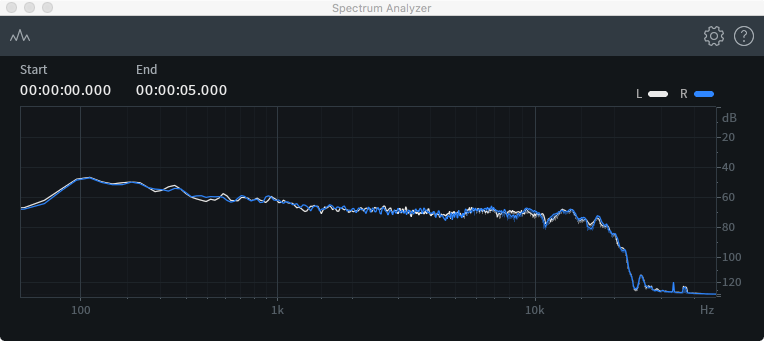
\includegraphics[width=.47\textwidth]{stereo-pairs-polar-patterns/PDF/AB.pdf}
% \caption{\textbf{AB}.}
% \label{AB}
% \end{center}
% \end{figure}
%-------------------------------------------------------------------------------
\subsubsection*{OSS}
% \vfill\null
% \begin{figure}[h]
% \begin{center}
% 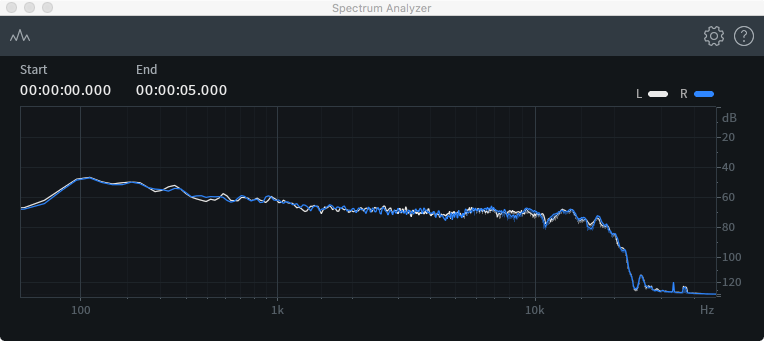
\includegraphics[width=.47\textwidth]{stereo-pairs-polar-patterns/PDF/AB.pdf}
% \caption{\textbf{AB}.}
% \label{AB}
% \end{center}
% \end{figure}
%-------------------------------------------------------------------------------
\subsubsection*{DECCA TREE}
% \vfill\null
% \begin{figure}[h]
% \begin{center}
% 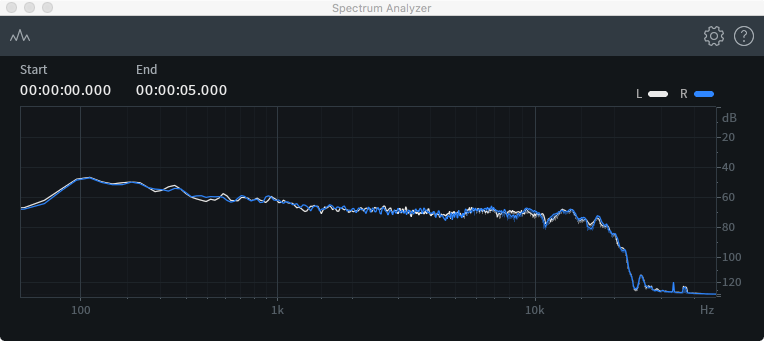
\includegraphics[width=.47\textwidth]{stereo-pairs-polar-patterns/PDF/AB.pdf}
% \caption{\textbf{AB}.}
% \label{AB}
% \end{center}
% \end{figure}
% \newpage % USE NEWPAGE TO FORCE COLUMNN INTERRUPTION
%-------------------------------------------------------------------------------
%-------------------------------------------------------------------------------
%\section*{UNNUMBERED SECTION}
%
% \begin{quote}
% La musica non e` solo composizione. \\
% Non è artigianato, non è un mestiere. \\
% La musica è pensiero. \cite{nono85}
% \end{quote}
%
% Some predictions of general relativity differ significantly from those of
% classical physics, especially concerning the passage of time, the geometry of
% space, the motion of bodies in free fall, and the propagation of light. Examples
% of such differences include gravitational time dilation, gravitational lensing,
% the gravitational redshift of light, and the gravitational time delay. The
% predictions of general relativity in relation to classical physics have been
% confirmed in all observations and experiments to date. Although general
% relativity is not the only relativistic theory of gravity, it is the simplest
% theory that is consistent with experimental data. However, unanswered questions
% remain, the most fundamental being how general relativity can be reconciled with
% the laws of quantum physics to produce a complete and self-consistent theory of
% quantum gravity.
%
% \begin{table}[htp]
% \begin{center}
% \begin{tabular}{ll}
% \textbf{Stages} & \textbf{Dur.} \\
% \hline
% \textbf{Omnidirectional Expositions} & 6 mo. \\
% Sound-shape analysis and visualizations & \\
% Sound-shape reproduction & \\
% Sound-shape database design & \\
% \hline
% \textbf{Micro-Rhythm of sound-shape} & 12 mo. \\
% Solo repertoire analysis & \\
% Sound-shape explosion in practising & \\
% From literature to shapes open-data & \\
% \hline
% \textbf{Rhythm of sound-shape interactions} & 12 mo. \\
% Multiple sources multiple shapes & \\
% Relationship and complexity perception & \\
% \hline
% \textbf{Sound-shape in musical composition} & 12 mo. \\
% AI: unleashed writing opportunities & \\
% AI: can you listen the time? & \\
% \hline
% \textbf{Final documentation} & 6 mo. \\
% \end{tabular}
% \label{timesheet}
% \caption{Thinking Tetrahedral Today stages}
% \end{center}
% \end{table}%
%
% Einstein's theory has important astrophysical implications. For example, it
% implies the existence of black holes regions of space in which space and time
% are distorted in such a way that nothing, not even light, can escape as an
% end state for massive stars. There is ample evidence that the intense radiation
% emitted by certain kinds of astronomical objects is due to black holes. For
% example, microquasars and active galactic nuclei result from the presence of
% stellar black holes and supermassive black holes, respectively. The bending of
% light by gravity can lead to the phenomenon of gravitational lensing, in which
% multiple images of the same distant astronomical object are visible in the sky.
% General relativity also predicts the existence of gravitational waves, which
% have since been observed directly by the physics collaboration LIGO. In addition,
% general relativity is the basis of current cosmological models of a consistently
% expanding universe. \cite{gerzon_70b}
%
% \begin{compactitem}
% \item Derivations of the Lorentz transformations
% \item Einstein–Hilbert action
% \item Tests of general relativity
% \item Two-body problem in general relativity
% \end{compactitem}
%
% \begin{figure}[t]
% \centering
% 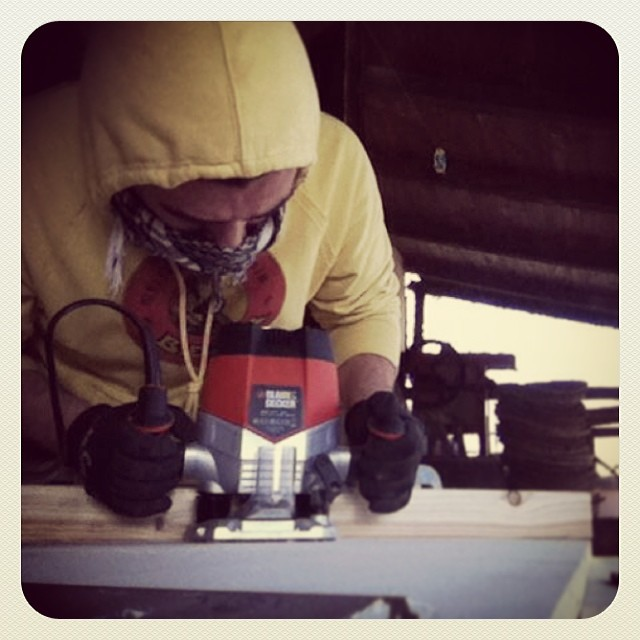
\includegraphics[width=.47\textwidth]{img/image2.jpg}
% \caption{Mind Mapping}
% \label{gs}
% \end{figure}
%
% \begin{equation}
% m(x,p,\theta) = (p*x) + ((1-p)*(x\cos\theta)
% \label{eq:mid}
% \end{equation}
%
% Some predictions of general relativity differ significantly from those of
% classical physics, especially concerning the passage of time, the geometry of
% space, the motion of bodies in free fall, and the propagation of light.

\clearpage
\section*{RILEVAZIONI SPERIMENTALI}

%% This file was created by matlab2tikz.
%
%The latest updates can be retrieved from
%  http://www.mathworks.com/matlabcentral/fileexchange/22022-matlab2tikz-matlab2tikz
%where you can also make suggestions and rate matlab2tikz.
%
\definecolor{mycolor1}{rgb}{0.00000,0.44700,0.74100}%
%
\begin{tikzpicture}

\begin{axis}[%
width=1.471in,
height=1.224in,
at={(2.6in,7.882in)},
scale only axis,
xmin=0,
xmax=1024,
xtick={\empty},
ymin=-100,
ymax=21.8264204267973,
ylabel style={font=\color{white!15!black}},
ylabel={01-ORTF SCHOEPS},
axis background/.style={fill=white},
title style={font=\bfseries},
title={135sx}
]
\addplot [color=mycolor1, forget plot]
  table[row sep=crcr]{%
1	-3.84317498797536\\
2	0.634569514910972\\
3	12.6940787050761\\
4	6.85796160034882\\
5	11.6678502599042\\
6	16.5670446642137\\
7	5.41564644242704\\
8	-19.6659068307189\\
9	8.64919181237774\\
10	7.43892729737951\\
11	1.72995832318043\\
12	-4.80479726575496\\
13	-2.81822109439149\\
14	-0.846834829291475\\
15	2.32615544751342\\
16	-3.58578390413319\\
17	0.0151565495664529\\
18	3.81891905723665\\
19	2.15363184937657\\
20	-5.76923163613261\\
21	-1.24717256720789\\
22	-3.97580917826064\\
23	0.803924396043776\\
24	-2.21997105447807\\
25	0.13465417584312\\
26	-5.0771158913524\\
27	-6.65571828785338\\
28	-2.75464109318152\\
29	-0.771165729714669\\
30	-0.107621920380802\\
31	-1.44323976658675\\
32	-9.49880946724518\\
33	-3.92046431288238\\
34	1.46788086748292\\
35	-11.4637775739785\\
36	-14.4169233061989\\
37	-5.30346767441125\\
38	-2.02023143239504\\
39	-0.321309443318248\\
40	-14.8104785329426\\
41	-7.96477336071554\\
42	-8.05026822861453\\
43	-6.29186885830981\\
44	-10.5179788736818\\
45	-5.52926029842336\\
46	-1.53652795166589\\
47	-9.56534362784558\\
48	-5.76358340055921\\
49	-3.36475399173437\\
50	-4.03832465706175\\
51	-17.2015145223065\\
52	-5.77789454885275\\
53	-4.62669661159222\\
54	-5.03969989750389\\
55	-1.98850623348871\\
56	-26.8136631130709\\
57	-22.6295969046723\\
58	-3.98129363828871\\
59	-6.59969008193993\\
60	-11.589483312434\\
61	-11.9892997249208\\
62	-9.13195754829482\\
63	-13.1379819758208\\
64	-6.3263198316291\\
65	-2.69997300520074\\
66	-6.3895865413012\\
67	-12.4440725768458\\
68	-16.4197081619715\\
69	-18.1471896275867\\
70	-7.55300829080283\\
71	-29.2998580304667\\
72	-12.8881856993064\\
73	-15.5535101668465\\
74	-16.0419659110409\\
75	-9.50212654801962\\
76	-1.58177252755683\\
77	-3.86958737772908\\
78	-14.1962845696358\\
79	-5.67485016364727\\
80	-2.48666705369253\\
81	1.10607551007949\\
82	-6.94371321318607\\
83	-3.28392501907916\\
84	-12.9776726357024\\
85	-11.5672669342349\\
86	-2.18559187917629\\
87	-4.8193916839508\\
88	-8.16805943445368\\
89	-11.1362575765155\\
90	-3.02372537371708\\
91	-9.00915584231317\\
92	-8.9438146928976\\
93	-13.6989742718983\\
94	-6.23597233591093\\
95	-6.39937674827387\\
96	-14.1487465166052\\
97	-10.8864812959466\\
98	-17.1148272459705\\
99	-23.5488864808688\\
100	-6.63605679195294\\
101	-11.3294502893399\\
102	-9.81922880611534\\
103	-16.4487294083156\\
104	-12.516491556658\\
105	-15.5063566030298\\
106	-25.4098898959544\\
107	-17.0926708188837\\
108	-9.59815204685183\\
109	-27.7055946047334\\
110	-9.01708565676565\\
111	-6.43683084316487\\
112	-21.2876215660694\\
113	-6.44452714065193\\
114	-11.3835856497268\\
115	-1.46243108142715\\
116	-8.12146226466149\\
117	-3.01544832796714\\
118	-12.2249437976996\\
119	-4.23254511961343\\
120	-10.9710095097605\\
121	-1.94695606598909\\
122	-12.9812365948913\\
123	-12.0147240594756\\
124	-8.50468997593973\\
125	-8.34627166960617\\
126	-7.22894534117788\\
127	-6.40857786463325\\
128	-4.09375758210875\\
129	-10.1292608425116\\
130	-9.21170926969521\\
131	-3.37788568669974\\
132	-1.74562761108175\\
133	-3.53340413578203\\
134	-19.610167573228\\
135	-14.0565037665709\\
136	-8.50600221703513\\
137	-17.6169684656872\\
138	-6.1627398677038\\
139	-12.2832558805248\\
140	-8.52805257361139\\
141	-3.13290115392383\\
142	-8.68680420318609\\
143	-0.583092728710399\\
144	-3.4722362543176\\
145	-9.73784643541947\\
146	-7.05809485449448\\
147	-6.96354685887535\\
148	-5.99326252746158\\
149	-10.037375661742\\
150	-11.6368740864349\\
151	-11.5030573717989\\
152	0.340713322640389\\
153	-20.0627041540776\\
154	-3.9864471126905\\
155	-10.1285627689193\\
156	-7.5921986539586\\
157	-10.5286968593721\\
158	-3.63721628575634\\
159	-20.3461419454015\\
160	-11.9168249235717\\
161	-15.4762368406068\\
162	-17.9141354977684\\
163	-4.83410579122784\\
164	-20.4648877834392\\
165	-4.93267125071637\\
166	-18.3316302861132\\
167	-25.9942824083601\\
168	-8.16249887960433\\
169	-0.762080529675907\\
170	-20.4868728585681\\
171	-6.0449293582544\\
172	-12.2998568659254\\
173	-9.1489317279431\\
174	-7.51956505996669\\
175	-8.33281569524816\\
176	-3.56927513246033\\
177	-6.83202753864681\\
178	-9.14054273048786\\
179	-22.0602723866276\\
180	-5.87393506713726\\
181	-10.5441550993167\\
182	-12.5812510919852\\
183	-7.21283188682926\\
184	-6.3261128968669\\
185	-23.2563809086101\\
186	-10.2813497697845\\
187	-13.0321995341707\\
188	-20.5947891194752\\
189	-22.0725205330997\\
190	-11.805356293423\\
191	-20.4815914261252\\
192	-8.88965704099658\\
193	-18.1891130342301\\
194	-11.8535371476384\\
195	-9.18144199421151\\
196	-7.81112664768782\\
197	-26.1158995950462\\
198	-22.118196010958\\
199	-8.29613577210969\\
200	-20.7932514129953\\
201	-19.4050316726895\\
202	-6.25529000213377\\
203	-22.0089682009749\\
204	-8.85692391481471\\
205	-11.1580333997085\\
206	-22.8489486833288\\
207	-20.6761171964387\\
208	-12.8930905467272\\
209	-5.07610927355811\\
210	-17.7564956132322\\
211	-23.9666618374271\\
212	-17.9940696664257\\
213	-13.5589068814617\\
214	-21.3678777353622\\
215	-4.67093287748799\\
216	-13.3925481169167\\
217	-13.5526814435439\\
218	-3.99125083884795\\
219	-27.7302327618317\\
220	-12.52466734258\\
221	-9.98451517207935\\
222	-8.37556163736297\\
223	-6.41000900342249\\
224	-2.98561019640339\\
225	-8.91897138198786\\
226	-6.12231571642317\\
227	-19.9216003425224\\
228	-14.8468741731535\\
229	-13.219464375299\\
230	-7.54348294468684\\
231	-10.2118212921139\\
232	-9.93707508732543\\
233	-8.74209423383997\\
234	-16.9048926743712\\
235	-10.6828420198944\\
236	-10.733827048799\\
237	-9.05235625300855\\
238	-7.89070109595421\\
239	-7.90770659139395\\
240	-9.57989292904394\\
241	-10.3024540358998\\
242	-9.40496889964993\\
243	-15.1827123139612\\
244	-12.3790900159541\\
245	-11.3126386828726\\
246	-13.7886016280591\\
247	-6.16312368997025\\
248	-10.2315030430934\\
249	-7.89275905882268\\
250	-24.9023476000485\\
251	-19.3014136955644\\
252	-7.81665317333164\\
253	-10.0779395720232\\
254	-12.292982686801\\
255	-15.6691667728317\\
256	-8.61836017699466\\
257	-7.19066612229632\\
258	-15.8421469750106\\
259	-21.9603141883561\\
260	-11.1379427090282\\
261	-10.5979474561573\\
262	-22.5533977081275\\
263	-8.75631501815142\\
264	-13.7745690736072\\
265	-8.67677028634453\\
266	-17.546857135627\\
267	-11.4119200025776\\
268	-15.5098450963394\\
269	-18.7798260564213\\
270	-24.6752054885405\\
271	-14.0720980306587\\
272	-15.81046071216\\
273	-9.28156811804906\\
274	-19.6937229434933\\
275	-15.4095379884774\\
276	-26.1816212025953\\
277	-28.6554543587052\\
278	-11.4607816577856\\
279	-19.5423971181814\\
280	-11.8628517269917\\
281	-21.3987128360163\\
282	-17.3017343836533\\
283	-9.7791233291151\\
284	-14.3826461531837\\
285	-17.4652197876071\\
286	-14.2646576524697\\
287	-9.50287374086896\\
288	-18.1304259249023\\
289	-13.6364038834673\\
290	-22.6587934189987\\
291	-15.4456301073299\\
292	-19.9196112205996\\
293	-11.8814592814209\\
294	-15.1829158654679\\
295	-20.2335435121025\\
296	-18.6375589031148\\
297	-14.6755497499783\\
298	-11.1492442724881\\
299	-21.2460399534417\\
300	-18.5040145661155\\
301	-21.0513211359355\\
302	-33.2313086297065\\
303	-15.5290868728664\\
304	-22.8553102368829\\
305	-25.6777485877607\\
306	-18.000010519082\\
307	-15.5327279114224\\
308	-15.5312749876984\\
309	-14.7256145571252\\
310	-24.7472149155921\\
311	-13.5672827235014\\
312	-19.3890472512306\\
313	-14.0824511861276\\
314	-20.1667431762674\\
315	-17.3539003855277\\
316	-10.6916267401901\\
317	-21.0339221691171\\
318	-21.8975008397939\\
319	-13.5196340998597\\
320	-21.037824387199\\
321	-18.87616028099\\
322	-14.4918320601703\\
323	-18.6145875477346\\
324	-11.5709978512473\\
325	-19.2100789899313\\
326	-15.8945148842358\\
327	-13.7341413519423\\
328	-10.5011642378253\\
329	-25.7275737580176\\
330	-12.8426913441181\\
331	-8.51770193287028\\
332	-14.6165861169769\\
333	-11.3583656542098\\
334	-7.94256876187846\\
335	-16.4881114455083\\
336	-21.9167599275068\\
337	-17.3253844215906\\
338	-27.4169019255993\\
339	-11.4660040107255\\
340	-9.3346772101933\\
341	-18.7901934520231\\
342	-11.1777549968196\\
343	-15.3043924120034\\
344	-14.0734387809161\\
345	-14.1545792011647\\
346	-12.8538429709645\\
347	-14.2231056683074\\
348	-28.9237936870276\\
349	-19.7027005968788\\
350	-28.3186470291296\\
351	-22.0837436400021\\
352	-25.4487946259492\\
353	-15.7757029603251\\
354	-19.0219937182966\\
355	-33.7812510337645\\
356	-19.1442357104633\\
357	-23.3309152304028\\
358	-23.7818456815961\\
359	-22.9099518460255\\
360	-20.0794920144536\\
361	-29.4593282187385\\
362	-26.2493599398424\\
363	-15.0888841174927\\
364	-13.4756500288479\\
365	-14.4951307315986\\
366	-25.539061210489\\
367	-14.8438779623814\\
368	-23.5816776360817\\
369	-19.1563440929103\\
370	-16.1878899741935\\
371	-16.5770818317341\\
372	-21.6610369050304\\
373	-26.3789762828459\\
374	-20.3526707939963\\
375	-27.7653192628115\\
376	-23.4033367616568\\
377	-37.1811752843271\\
378	-19.5762117906353\\
379	-26.6772862601662\\
380	-18.3521950429795\\
381	-16.8866767095058\\
382	-18.8369223613315\\
383	-23.9693354986891\\
384	-15.1072840685149\\
385	-20.9054310187439\\
386	-23.1431253255333\\
387	-17.7299056099644\\
388	-29.0022193955723\\
389	-22.652686326107\\
390	-15.6132154467664\\
391	-22.4399628505304\\
392	-33.5750861558325\\
393	-20.87886036449\\
394	-25.0622235982003\\
395	-28.6501082796034\\
396	-30.5631176352354\\
397	-16.652376582648\\
398	-20.544853495213\\
399	-23.8886316249601\\
400	-30.8947599790573\\
401	-30.0220835430128\\
402	-39.7568683242759\\
403	-33.5602711819194\\
404	-27.1022947066533\\
405	-25.8507824134199\\
406	-30.7089968135584\\
407	-36.0834083987009\\
408	-26.4310042095012\\
409	-27.1215569806402\\
410	-41.2506003526669\\
411	-26.6636618761788\\
412	-43.2227291584284\\
413	-34.6920121976935\\
414	-30.8844183075577\\
415	-27.963932493254\\
416	-31.874923325679\\
417	-24.321774390736\\
418	-33.3151037058781\\
419	-24.1920684468998\\
420	-36.4355387908225\\
421	-27.2613155173712\\
422	-28.6932388150873\\
423	-32.2946167889744\\
424	-34.861622518858\\
425	-30.5177071075219\\
426	-25.4469670923659\\
427	-28.440101742649\\
428	-26.4010410089462\\
429	-36.1461411900995\\
430	-31.6939427250384\\
431	-36.9562855699897\\
432	-36.6085127583804\\
433	-29.6079652985058\\
434	-31.8892372441788\\
435	-34.077027318268\\
436	-33.5506824517978\\
437	-38.1266334996868\\
438	-33.6675654058924\\
439	-35.1746770493119\\
440	-34.5334185058687\\
441	-32.5635864583005\\
442	-31.481406235075\\
443	-36.795823178019\\
444	-33.559939356906\\
445	-38.7736349409102\\
446	-34.4475366771658\\
447	-35.3496474650584\\
448	-35.7971949695929\\
449	-34.1112799757057\\
450	-33.2631296895524\\
451	-33.9487779770843\\
452	-43.0534267517336\\
453	-33.3807465122717\\
454	-33.5865558571423\\
455	-38.4274841224684\\
456	-35.497251078825\\
457	-35.2909431207969\\
458	-36.7235783823149\\
459	-37.5928685301591\\
460	-42.4264287496366\\
461	-33.7472447165108\\
462	-40.2957662474012\\
463	-36.6805373100126\\
464	-38.9886114009655\\
465	-40.0355272506313\\
466	-37.2149847220288\\
467	-37.8544298079746\\
468	-33.8086882619803\\
469	-36.346665962326\\
470	-36.9085540476577\\
471	-36.507410386208\\
472	-36.6412162640274\\
473	-34.7200652338942\\
474	-37.4767353918048\\
475	-34.6225845184878\\
476	-36.4297772672527\\
477	-35.5189027498679\\
478	-37.2014134931101\\
479	-36.4985809196199\\
480	-36.9214796093426\\
481	-36.0126629475099\\
482	-36.307286644695\\
483	-36.9498279460143\\
484	-36.9909145601\\
485	-36.9818454285187\\
486	-36.2255296291189\\
487	-37.2035230559146\\
488	-37.6488708393241\\
489	-36.7704242844663\\
490	-37.5100081096124\\
491	-37.2482421134463\\
492	-37.365471946424\\
493	-37.2612193404319\\
494	-37.1515548452275\\
495	-37.4980602188698\\
496	-37.5877438638391\\
497	-37.5261763907759\\
498	-37.2985476805597\\
499	-37.9783809644043\\
500	-37.4590536915389\\
501	-37.746225102674\\
502	-37.832951092677\\
503	-38.0249060639127\\
504	-37.8243461955202\\
505	-37.7870297399773\\
506	-37.6957851612245\\
507	-37.7067784432539\\
508	-37.8291581471106\\
509	-37.8018842492242\\
510	-38.0325262939014\\
511	-37.9042186801459\\
512	-38.034681361595\\
513	-37.9349075994501\\
514	-38.0327817711015\\
515	-38.2543966237625\\
516	-38.0157331479054\\
517	-38.0660441041864\\
518	-37.9344677444807\\
519	-38.2418238985132\\
520	-38.1530754249147\\
521	-38.2078767651174\\
522	-38.011395579506\\
523	-38.4556742055202\\
524	-37.9837760065166\\
525	-38.2873877364077\\
526	-38.1948314842388\\
527	-38.274681879322\\
528	-38.9224341093679\\
529	-38.3725956969269\\
530	-38.5367770292508\\
531	-38.2702183488853\\
532	-38.348981661122\\
533	-38.3761169381213\\
534	-38.3816167647881\\
535	-38.3994747703681\\
536	-38.5872133625609\\
537	-38.34578470281\\
538	-38.5136741107245\\
539	-38.6761107722798\\
540	-38.4228716385738\\
541	-38.4638738881749\\
542	-38.5591787375133\\
543	-38.237016134718\\
544	-38.8578724492784\\
545	-38.7311101639287\\
546	-38.5660824975432\\
547	-38.7190982623949\\
548	-38.639740545701\\
549	-39.1166348871468\\
550	-38.7789961743713\\
551	-38.6988696279438\\
552	-38.7687513183784\\
553	-38.8954765648707\\
554	-38.7606114802309\\
555	-39.0029918945005\\
556	-38.7859663997635\\
557	-38.6816545654338\\
558	-38.6892559195449\\
559	-38.6819411317062\\
560	-38.8535892664481\\
561	-39.2010344067069\\
562	-38.9208231518987\\
563	-38.8287158962929\\
564	-38.9695003824655\\
565	-38.9747043149997\\
566	-38.9482427096754\\
567	-38.9073789491217\\
568	-39.248240086096\\
569	-39.2831875375887\\
570	-39.1515189184141\\
571	-39.1103957179343\\
572	-39.0619951773519\\
573	-38.970337959439\\
574	-39.1029412354302\\
575	-39.1163708845879\\
576	-39.1457076116696\\
577	-38.9437296809113\\
578	-39.0775166542986\\
579	-39.0768602866714\\
580	-39.2909900493056\\
581	-39.3125765164562\\
582	-39.1170614972567\\
583	-39.3639099782626\\
584	-39.5050547318057\\
585	-39.4835479703419\\
586	-39.4090679536331\\
587	-39.4489265748959\\
588	-39.2228621425596\\
589	-39.1460322943568\\
590	-39.477288222876\\
591	-39.5073487659492\\
592	-39.3664778830887\\
593	-39.177662580362\\
594	-39.445301054661\\
595	-39.3122711752394\\
596	-39.360771289845\\
597	-39.6872099663702\\
598	-39.5340993848589\\
599	-39.4432053021457\\
600	-39.6152114761047\\
601	-39.7195712624261\\
602	-39.6182810808301\\
603	-39.6676126591032\\
604	-39.6326728979531\\
605	-39.6910935775267\\
606	-39.5824769745497\\
607	-39.7203856431287\\
608	-39.8658593606546\\
609	-39.7174045142205\\
610	-39.6614761210691\\
611	-39.5897152816553\\
612	-39.6557802942994\\
613	-39.6681763542645\\
614	-39.7977352976755\\
615	-39.781401200065\\
616	-39.6157655209322\\
617	-39.7996632004042\\
618	-40.0678162592167\\
619	-39.7376764302796\\
620	-39.730172409606\\
621	-39.7058983595053\\
622	-39.6330800167802\\
623	-39.9837293187072\\
624	-39.8131541861831\\
625	-39.8863138046284\\
626	-39.7990041427659\\
627	-39.9269621124897\\
628	-39.8122789553399\\
629	-39.9759371773231\\
630	-39.979103472875\\
631	-40.1708046218312\\
632	-39.8553618020428\\
633	-39.9700043478194\\
634	-40.0457437619726\\
635	-39.8922021363937\\
636	-40.282121249415\\
637	-39.966764313885\\
638	-40.0305001698972\\
639	-39.9935312226127\\
640	-40.1579256999308\\
641	-39.9509616650187\\
642	-40.0375190309567\\
643	-40.010595676201\\
644	-40.1768129150214\\
645	-40.2276670497696\\
646	-40.3545364642632\\
647	-40.1306443735049\\
648	-40.1448149145906\\
649	-40.4726184208071\\
650	-40.3990311170426\\
651	-40.2620309342223\\
652	-40.0165319512407\\
653	-40.4292070563491\\
654	-40.2862440207591\\
655	-40.3098986104334\\
656	-40.2836052462227\\
657	-40.2039928407\\
658	-40.5224278844244\\
659	-40.439482217275\\
660	-40.2930848200185\\
661	-40.5233527279098\\
662	-40.1927370557825\\
663	-40.4641663576587\\
664	-40.3107427456623\\
665	-40.2933586585053\\
666	-40.3665690182935\\
667	-40.4981849974167\\
668	-40.4275168819975\\
669	-40.435139002719\\
670	-40.1774976772067\\
671	-40.4658460620712\\
672	-40.4967105601162\\
673	-40.6354678359825\\
674	-40.4637869719436\\
675	-40.5010012990802\\
676	-40.442774140087\\
677	-40.331238829626\\
678	-40.6071549412382\\
679	-40.5664210046786\\
680	-40.5720065731448\\
681	-40.6537952269707\\
682	-40.6603994730565\\
683	-40.5645069813008\\
684	-40.7640008150404\\
685	-40.4910584248894\\
686	-40.5466713449437\\
687	-40.4679830138098\\
688	-40.3951012065636\\
689	-40.6155075665688\\
690	-40.8850066196435\\
691	-40.6512664376067\\
692	-40.7387301204592\\
693	-40.666139656954\\
694	-40.8276442062937\\
695	-41.0374574735485\\
696	-40.5754205248157\\
697	-40.3305121629933\\
698	-40.5363057433116\\
699	-40.5537970352755\\
700	-40.9849029159757\\
701	-40.6065699246555\\
702	-40.8602226904003\\
703	-40.7602012761011\\
704	-40.7402364221067\\
705	-40.642791123417\\
706	-40.9156353358476\\
707	-40.7502853119479\\
708	-40.7774752438099\\
709	-40.8059437275523\\
710	-40.6165218298272\\
711	-40.7950878977519\\
712	-40.9240937670108\\
713	-40.9793675721807\\
714	-40.9860144564133\\
715	-40.9043328457218\\
716	-40.7909394720694\\
717	-40.8247560927617\\
718	-41.0665565971978\\
719	-41.0162790032913\\
720	-41.1382854803877\\
721	-41.06229441767\\
722	-40.9490897594687\\
723	-40.8431729267227\\
724	-41.0916329511055\\
725	-40.9849848425933\\
726	-40.9881957497826\\
727	-40.8400041373686\\
728	-41.1888718154446\\
729	-41.0137830332647\\
730	-40.9412495523129\\
731	-40.9985516056737\\
732	-40.8018075973581\\
733	-41.281171520973\\
734	-41.050234472614\\
735	-41.0534233032155\\
736	-41.1415299258511\\
737	-41.0249843286428\\
738	-41.1441161112653\\
739	-41.0471976769618\\
740	-41.1413128152504\\
741	-41.2866823719618\\
742	-41.2367145711224\\
743	-41.036195175088\\
744	-41.0750861244445\\
745	-41.0818954299064\\
746	-41.1753668128429\\
747	-40.9206254382099\\
748	-41.0454536873902\\
749	-40.8791182001738\\
750	-41.0667946855503\\
751	-41.1404923985254\\
752	-41.2506984075389\\
753	-41.2354286183268\\
754	-41.1808990929196\\
755	-41.2707193672591\\
756	-41.1811214449173\\
757	-41.1356520431941\\
758	-40.9250882518301\\
759	-41.2660557436925\\
760	-41.1885420603401\\
761	-41.206447322711\\
762	-41.1875556584186\\
763	-41.4910518413807\\
764	-41.2791785223517\\
765	-41.4318898209324\\
766	-41.1327447474009\\
767	-41.4168541841579\\
768	-41.4042251754579\\
769	-41.4229443118127\\
770	-41.3179008493521\\
771	-41.4355442614414\\
772	-41.2369161024117\\
773	-41.1568184150698\\
774	-41.2412640973537\\
775	-41.0983994314373\\
776	-41.0166063501884\\
777	-41.429428425476\\
778	-41.3486218785629\\
779	-41.5016501018211\\
780	-41.3390168392783\\
781	-41.7275449130082\\
782	-41.4491430815608\\
783	-41.2994630648229\\
784	-41.3215997156699\\
785	-41.3045133729158\\
786	-41.6103541796723\\
787	-41.5075740122596\\
788	-41.8788698539839\\
789	-41.591031233939\\
790	-41.4506732839153\\
791	-41.6446749893642\\
792	-41.3458355035148\\
793	-41.544719164867\\
794	-41.4046706118398\\
795	-41.6590453542148\\
796	-41.4895946135313\\
797	-41.5960258434761\\
798	-41.2751660535533\\
799	-41.4295572455422\\
800	-41.6300281958729\\
801	-41.3393484128216\\
802	-41.7151999454531\\
803	-41.5864251243627\\
804	-41.5657249777509\\
805	-41.7731545399567\\
806	-41.5937509448261\\
807	-41.6384127555034\\
808	-41.7837535010458\\
809	-41.6218041552508\\
810	-41.5302412374571\\
811	-41.565700397379\\
812	-41.6944897581966\\
813	-41.877165714025\\
814	-41.4969900364325\\
815	-41.8505165575528\\
816	-41.6580150493309\\
817	-41.7070586268239\\
818	-41.6235362098523\\
819	-41.592333156568\\
820	-41.672727962045\\
821	-41.8538266315828\\
822	-41.4084697778081\\
823	-41.6114475507128\\
824	-41.6470261258482\\
825	-41.5221367595277\\
826	-41.8031444730271\\
827	-41.7601996997844\\
828	-41.8976638018236\\
829	-41.7373165649903\\
830	-41.6498739615796\\
831	-41.7142016983924\\
832	-41.8984433671253\\
833	-41.6299467286841\\
834	-41.870366360976\\
835	-41.7193479458151\\
836	-41.8672683279187\\
837	-41.7644670997822\\
838	-41.8117726089231\\
839	-42.0223557973466\\
840	-41.5108725567028\\
841	-41.7903040731937\\
842	-41.7427459182294\\
843	-41.769950671866\\
844	-41.6968457379818\\
845	-41.8189280679161\\
846	-41.9658234053901\\
847	-41.5861162874435\\
848	-41.7489358229645\\
849	-41.8546740859903\\
850	-41.5798945171922\\
851	-41.9565819089466\\
852	-41.5584549469556\\
853	-41.8754750538657\\
854	-41.8714659208764\\
855	-42.0368790734249\\
856	-41.7125974625818\\
857	-41.7170868290679\\
858	-41.7441228183265\\
859	-41.8526626534503\\
860	-41.673075476445\\
861	-41.7580392601778\\
862	-41.7355762191451\\
863	-41.808975354752\\
864	-41.9925435740797\\
865	-41.7858032032212\\
866	-41.8272561904168\\
867	-41.8169331038749\\
868	-41.7768845554754\\
869	-41.7327172740008\\
870	-41.9113575182008\\
871	-41.9499764605213\\
872	-41.8218827126576\\
873	-41.8759325552382\\
874	-41.8307397584835\\
875	-41.6687038898007\\
876	-42.0281367344121\\
877	-41.9635486526242\\
878	-41.8320588086411\\
879	-41.878589498827\\
880	-41.8857526600454\\
881	-41.8637061961475\\
882	-41.6874447228746\\
883	-41.6495700735372\\
884	-41.7667887385062\\
885	-42.0305991280573\\
886	-41.9665956246059\\
887	-42.0506895460153\\
888	-41.9242173661409\\
889	-41.7469513704975\\
890	-42.1588280580173\\
891	-41.8115425096873\\
892	-42.0414340708752\\
893	-41.9959117148524\\
894	-42.0955546170696\\
895	-42.0900217770315\\
896	-41.8891694349822\\
897	-41.9812077573255\\
898	-41.9626983715672\\
899	-41.9696946958313\\
900	-42.1347791793267\\
901	-41.9313620313014\\
902	-42.0204942108214\\
903	-42.0305747066368\\
904	-42.0323045346632\\
905	-41.9170322764794\\
906	-41.7899379323778\\
907	-42.189581639113\\
908	-42.020000935164\\
909	-42.0121093761853\\
910	-42.0982651058571\\
911	-42.0652023175931\\
912	-41.9639219337525\\
913	-42.3321753195854\\
914	-42.2050555240167\\
915	-42.0950731383069\\
916	-42.1164625385206\\
917	-42.1209310512509\\
918	-42.0091988672392\\
919	-41.9922636216501\\
920	-42.1395853749275\\
921	-42.0361707826134\\
922	-42.1292458558405\\
923	-42.15551464415\\
924	-42.1657396483099\\
925	-41.9000397513884\\
926	-42.2343366085528\\
927	-42.1247488339\\
928	-42.0103126791023\\
929	-42.2227861728629\\
930	-41.9387131077358\\
931	-42.0505506745165\\
932	-42.0427393602031\\
933	-42.2389036346089\\
934	-42.0689569972404\\
935	-42.0224959347696\\
936	-42.1967574088665\\
937	-41.9750389398321\\
938	-41.8189267107472\\
939	-42.0717965227001\\
940	-42.1420779080517\\
941	-42.1776654403317\\
942	-42.2536807617733\\
943	-42.0184421526604\\
944	-42.0572458671981\\
945	-42.124027028051\\
946	-42.1390855019434\\
947	-42.1107345974888\\
948	-42.1650683862976\\
949	-42.0613559048668\\
950	-42.1031190853175\\
951	-42.1300908934949\\
952	-41.9964116461835\\
953	-42.2594002072238\\
954	-42.171110478762\\
955	-42.1800170684994\\
956	-41.967728704496\\
957	-42.0304763007228\\
958	-42.0847451445111\\
959	-41.9960095537814\\
960	-42.0230622448565\\
961	-42.1115249206083\\
962	-42.1295445767144\\
963	-42.2143152220967\\
964	-42.2997394540808\\
965	-42.1195455835184\\
966	-41.9376919563932\\
967	-42.3147665068924\\
968	-42.2133583117891\\
969	-42.0353880818141\\
970	-42.292161662331\\
971	-41.9623968459781\\
972	-42.0877666444301\\
973	-42.1847966739927\\
974	-42.4130895337899\\
975	-42.1058524988675\\
976	-42.165811721873\\
977	-42.1255538092841\\
978	-41.9674621286887\\
979	-42.2655216565666\\
980	-42.0165991466267\\
981	-42.0610670679475\\
982	-42.1504343074013\\
983	-42.1136563924616\\
984	-42.0535343144782\\
985	-42.0512514534119\\
986	-42.3157350401274\\
987	-42.109464225314\\
988	-41.950301124462\\
989	-41.9449989528258\\
990	-42.2151768923297\\
991	-42.3547051814191\\
992	-42.1335916040248\\
993	-42.3296568567471\\
994	-42.0498588839545\\
995	-42.1489868497365\\
996	-42.0184162554181\\
997	-42.1322098224612\\
998	-42.2221961108656\\
999	-42.0951277059933\\
1000	-42.2388225142272\\
1001	-42.2319394750714\\
1002	-42.0454186226291\\
1003	-42.1756725965633\\
1004	-42.0195583537016\\
1005	-41.9979039804681\\
1006	-42.2377245397814\\
1007	-42.2178195245271\\
1008	-42.4148317556217\\
1009	-42.1663846851931\\
1010	-42.0660604820784\\
1011	-42.029251390454\\
1012	-42.2287922406127\\
1013	-42.1339502297478\\
1014	-42.0814046011797\\
1015	-42.2839066307068\\
1016	-42.4346518117849\\
1017	-42.2241369202079\\
1018	-42.0454615464038\\
1019	-42.2650011091315\\
1020	-42.2502727807154\\
1021	-42.1558649824291\\
1022	-42.2140345702641\\
1023	-42.077700096001\\
1024	-42.133582441791\\
};
\end{axis}

\begin{axis}[%
width=1.471in,
height=1.224in,
at={(4.597in,7.882in)},
scale only axis,
xmin=0,
xmax=1024,
xtick={\empty},
ymin=-100,
ymax=21.8264204267973,
ytick={\empty},
axis background/.style={fill=white},
title style={font=\bfseries},
title={90sx}
]
\addplot [color=mycolor1, forget plot]
  table[row sep=crcr]{%
1	-18.8803907927792\\
2	1.41413853920182\\
3	-0.95626492857134\\
4	15.5356094631882\\
5	10.8984788346105\\
6	5.24232170960225\\
7	10.7739722595625\\
8	5.11477988557029\\
9	1.84027522451323\\
10	8.42491945966171\\
11	-3.10254069155941\\
12	3.67485371476014\\
13	5.94658054292879\\
14	4.6508220803638\\
15	2.43041496744449\\
16	2.67050336400938\\
17	0.0140583142736928\\
18	-1.16950928771464\\
19	-1.67417983289135\\
20	7.22398737646717\\
21	8.96485392617005\\
22	3.71083466902265\\
23	2.5226680561718\\
24	1.63945950976731\\
25	6.24476946767649\\
26	-6.01356090647582\\
27	4.13293501562989\\
28	3.2728032877887\\
29	-0.35963830954255\\
30	-1.14358997184661\\
31	-7.21909719419159\\
32	-2.88762784181952\\
33	-0.306647286055357\\
34	0.692505397593722\\
35	-1.77306488683485\\
36	-5.07593682604572\\
37	-7.93280580726396\\
38	-10.3025667520709\\
39	-1.07151840130276\\
40	-9.57403571718689\\
41	-2.64715496893253\\
42	-2.39309170794291\\
43	3.90381460967304\\
44	1.525121814009\\
45	-2.34477814904343\\
46	2.37924262681783\\
47	-2.16678686761058\\
48	-5.83121585060471\\
49	-10.0176770796036\\
50	-4.82047696352511\\
51	-7.02963281896776\\
52	-0.492730774143409\\
53	-0.521573401016116\\
54	2.66830320754622\\
55	-6.40301913959618\\
56	-9.67212519952614\\
57	0.258672423057156\\
58	-0.368351315249697\\
59	-18.5155877527968\\
60	-2.51985899099735\\
61	-4.35425161686307\\
62	-8.35754665753357\\
63	-3.29822576777488\\
64	-1.80816218124734\\
65	-4.11904652249006\\
66	-3.87281646110157\\
67	-13.6431899309917\\
68	-0.569478508629071\\
69	-6.79923238641254\\
70	-6.53675740293124\\
71	-5.43295080327328\\
72	-5.3263234047106\\
73	-2.89883043405758\\
74	-0.612492821273018\\
75	-4.68129736056565\\
76	1.51852788577397\\
77	-9.11518325992713\\
78	-3.6771323199675\\
79	-7.99849154189349\\
80	-3.82614503104665\\
81	-6.30676284077027\\
82	-2.3345030484957\\
83	-4.32129261987856\\
84	-2.86305166539677\\
85	1.79267437473606\\
86	-3.85073086450939\\
87	-3.18113437079305\\
88	-11.4815965569934\\
89	-1.46381708000277\\
90	-7.10084345274987\\
91	-12.7630041983645\\
92	-13.8208555541885\\
93	-7.82619561288303\\
94	-3.39425349617076\\
95	-0.90640559270351\\
96	-2.89893103149898\\
97	0.148375012599822\\
98	-18.3365032410794\\
99	-12.9990943773242\\
100	-5.07590564974935\\
101	-3.34240557981415\\
102	-11.3783673435408\\
103	-14.9050997871515\\
104	-6.81160222960659\\
105	-11.1097563773617\\
106	-4.74045775279443\\
107	-32.2156061450033\\
108	-2.48759629749201\\
109	-4.99270974396106\\
110	2.79451852907301\\
111	-4.08062646143889\\
112	-6.18173462023712\\
113	0.82381864806514\\
114	-7.34334490491567\\
115	-9.48559626329933\\
116	-3.666991057874\\
117	-7.89517740228217\\
118	-17.8515976745846\\
119	-12.3493601056563\\
120	-6.56312346121554\\
121	3.17940092536914\\
122	2.23632560658365\\
123	0.611178971811553\\
124	-10.2140644387908\\
125	3.11247191517149\\
126	0.7258287480882\\
127	-4.90204821647156\\
128	-2.7948978065258\\
129	4.96694941324958\\
130	0.754852264817717\\
131	-3.80569087806808\\
132	-4.05165823004462\\
133	4.10737228624611\\
134	-4.71304339722152\\
135	-10.3652469037957\\
136	-4.67749330268363\\
137	0.474853791842009\\
138	-13.273036466094\\
139	3.53178868317579\\
140	-10.4804925231355\\
141	-4.88410967879628\\
142	-0.27031615161756\\
143	-0.285623299596519\\
144	-0.648857966436785\\
145	-7.33373648967326\\
146	-7.6151055236163\\
147	-3.38582053238254\\
148	-0.492920965233841\\
149	-2.81541464464016\\
150	0.584174486095783\\
151	-13.2138150029307\\
152	-8.74094504330357\\
153	3.09568794433769\\
154	-6.68169154595771\\
155	-3.05894154520488\\
156	0.493119126302648\\
157	-2.3918176823702\\
158	-0.297714173959313\\
159	-13.8968141773078\\
160	-11.6803435512915\\
161	0.967923713976356\\
162	-10.3303642850896\\
163	0.587290065518312\\
164	-3.08460883165372\\
165	-8.09227630674883\\
166	-11.4391986591484\\
167	-1.97652782589182\\
168	1.06377733954854\\
169	-6.81191393232888\\
170	-4.02300851654582\\
171	-6.39268420997179\\
172	-4.05895202562985\\
173	-12.0618986321412\\
174	-2.80267866891915\\
175	-1.61973864069533\\
176	-4.56937792183911\\
177	-11.9266648447158\\
178	-6.38855786551281\\
179	-4.3176342979496\\
180	-7.53433343920269\\
181	-8.99031247497391\\
182	-13.0452066771226\\
183	-6.16631970928178\\
184	-3.67572333407842\\
185	-2.82926982247654\\
186	-3.22206346658196\\
187	-15.3728578997704\\
188	-10.5439751235188\\
189	-4.94568376734965\\
190	-6.87341569829469\\
191	-12.1163553019472\\
192	-14.9572057573228\\
193	-7.53549121359682\\
194	-7.69022310117245\\
195	-9.79878374265263\\
196	-14.8005291484042\\
197	-8.92550635827297\\
198	-16.129338597892\\
199	-24.0137587727764\\
200	-8.55347041646708\\
201	-13.8855455427177\\
202	-10.5170842112452\\
203	-3.23432757195104\\
204	-10.9699919006988\\
205	-15.9267000271156\\
206	-6.97857809349369\\
207	-7.25169027152232\\
208	0.578889619772306\\
209	-3.28091441279607\\
210	-2.76508854118576\\
211	0.172916340688282\\
212	-5.04743012550541\\
213	-4.339326089309\\
214	-3.40786456580687\\
215	1.12151268655047\\
216	-4.76432027305361\\
217	-12.5216753744486\\
218	-6.53976143459513\\
219	3.54484672246958\\
220	3.84500450776369\\
221	1.64248452957236\\
222	-2.18486205905903\\
223	-3.76384965099667\\
224	-8.91335410131009\\
225	2.86715055402905\\
226	-13.4958618164243\\
227	-6.0028431247814\\
228	-0.141670469226379\\
229	-10.845586856762\\
230	-10.2600068779055\\
231	2.00397243425332\\
232	1.55906311894701\\
233	3.00706399615823\\
234	-0.806834587895349\\
235	5.86660789291492\\
236	-13.2832547341449\\
237	-2.98161328105813\\
238	-3.43676927307136\\
239	-16.4376431254687\\
240	-0.666820385412801\\
241	3.34483846639233\\
242	6.85420004384599\\
243	6.32176770782689\\
244	-17.1185891871427\\
245	-2.32219600371715\\
246	0.759395061513612\\
247	0.344681223494697\\
248	-3.65673001469097\\
249	-4.04104102771805\\
250	-6.6210876323824\\
251	1.54907044801669\\
252	-3.71549511444246\\
253	-2.10950267709491\\
254	-10.8555412240432\\
255	-7.67950324768033\\
256	-11.2396257748154\\
257	-12.2414293473539\\
258	-6.05306533985622\\
259	-3.5506821636396\\
260	-6.12123310051264\\
261	-8.42582709658062\\
262	-1.57050315878745\\
263	-13.7897745550727\\
264	-0.235467013138661\\
265	-15.766776300592\\
266	0.459736931689317\\
267	2.61271232123764\\
268	1.33568768458774\\
269	-5.83366882622179\\
270	-4.92412719118018\\
271	-9.86305087137334\\
272	-4.30431099095005\\
273	-7.47467591204936\\
274	-9.08614073858977\\
275	-5.63106552906431\\
276	-10.4582955525121\\
277	-9.2382985794432\\
278	-7.43476584458316\\
279	-2.51815436640662\\
280	-7.34912277774463\\
281	-16.6790874728292\\
282	-10.3549085990046\\
283	-4.77795151352773\\
284	-6.77666147215861\\
285	-10.8701044815879\\
286	-14.4349915602818\\
287	-12.4028310624196\\
288	-12.4329143535539\\
289	-5.11161963205124\\
290	-8.73689761010029\\
291	-4.24233630007235\\
292	-11.8362250896009\\
293	-14.7553395491188\\
294	-5.06621125944131\\
295	-23.1719350755618\\
296	-11.5261182604229\\
297	-5.28080736264516\\
298	-19.6663373575522\\
299	-8.58520508682522\\
300	-6.93767503192271\\
301	-20.211773071448\\
302	-14.2366092913412\\
303	-18.5370939199257\\
304	-10.1904695959546\\
305	-13.4679590607703\\
306	-10.7312765453709\\
307	-17.9363104667743\\
308	-11.5185243372343\\
309	-17.5240776742001\\
310	-10.984305764373\\
311	-19.0432167584012\\
312	-11.400698634482\\
313	-5.15072782815565\\
314	-12.0201820863031\\
315	-12.8354287508761\\
316	-15.2204447396406\\
317	-9.6518678349542\\
318	-14.9639529825983\\
319	-5.65092135327133\\
320	-18.4606615583113\\
321	-6.02609949702034\\
322	-8.8015870783455\\
323	-6.04110627830312\\
324	-12.0100872046475\\
325	-8.69246296895078\\
326	-9.27648137470978\\
327	-9.04232649772986\\
328	-14.8803248715549\\
329	-25.2931488445472\\
330	-10.3093467188957\\
331	-12.6757240092405\\
332	-4.07852387106969\\
333	-10.0238488153128\\
334	-10.9064121502381\\
335	-22.4620935908925\\
336	-6.1684435616044\\
337	-12.2292177458766\\
338	-13.9141276690817\\
339	-6.159323222411\\
340	-6.21046893329895\\
341	-5.37013200273504\\
342	-5.63660196922652\\
343	2.80374542740573\\
344	-7.22535904819901\\
345	-10.5018028858196\\
346	-4.21880951669277\\
347	-24.9460281608512\\
348	-6.20983611199923\\
349	-17.0553801552473\\
350	-6.82295942670412\\
351	-3.8362423317129\\
352	-8.96862606522066\\
353	-8.08546041989244\\
354	-11.2000490999801\\
355	-7.0323657896782\\
356	-4.74776001837251\\
357	-17.5068606112003\\
358	-33.870623234885\\
359	-6.77041597554589\\
360	-13.2283616285369\\
361	-6.68811281706968\\
362	-9.66114901614981\\
363	-7.23017471807851\\
364	-4.42431318450093\\
365	-6.71449424842941\\
366	-10.0802725602391\\
367	-22.2168899689257\\
368	-29.0452925997892\\
369	-19.7446787632588\\
370	-7.07134147936891\\
371	-8.86517511588617\\
372	-12.7609378881546\\
373	-9.97561622192281\\
374	-7.44629138189212\\
375	-9.92136765013966\\
376	-8.75150674609451\\
377	-15.0696247502422\\
378	-9.88887333901354\\
379	-30.0886108225994\\
380	-15.4558575454619\\
381	-6.9149505170185\\
382	-6.1709216311975\\
383	-15.3344354680286\\
384	-18.6674995916325\\
385	-20.8131918867441\\
386	-14.0132485770733\\
387	-14.4580035374019\\
388	-16.726602780579\\
389	-20.1543139091097\\
390	-18.2937479130812\\
391	-21.2957727980513\\
392	-11.5964261465695\\
393	-19.1985382788052\\
394	-28.8313826724703\\
395	-17.0802998654235\\
396	-13.7003874423998\\
397	-20.8715949771812\\
398	-21.0360723951983\\
399	-30.7005282636923\\
400	-29.3179168944025\\
401	-33.5690638360126\\
402	-29.9678761622138\\
403	-20.3443971305066\\
404	-23.2531677594893\\
405	-23.8555081227199\\
406	-18.8039607251075\\
407	-27.3530872336501\\
408	-26.7079705780565\\
409	-18.3909240937647\\
410	-20.0886608691791\\
411	-18.8865127523624\\
412	-15.7351085461231\\
413	-17.9784658377679\\
414	-21.923351762663\\
415	-28.821229796312\\
416	-18.1159448365009\\
417	-18.8394016848574\\
418	-13.2921297703453\\
419	-29.1953117203205\\
420	-33.0434597150908\\
421	-30.8173500358163\\
422	-28.2250057882918\\
423	-19.2329205692379\\
424	-22.6074387962869\\
425	-20.5375146591043\\
426	-25.7691202270284\\
427	-20.9708688883425\\
428	-32.835136461859\\
429	-18.889713446636\\
430	-24.9277429173419\\
431	-26.703475459838\\
432	-27.2129912973508\\
433	-17.990829065266\\
434	-24.3130381983256\\
435	-20.865515690345\\
436	-23.3998229780361\\
437	-21.4173701859325\\
438	-26.7736141305862\\
439	-26.2478066745892\\
440	-26.3060132488975\\
441	-27.610162463766\\
442	-32.7634131403284\\
443	-34.2625972972473\\
444	-25.9536381335573\\
445	-26.2282755422173\\
446	-29.6424218623862\\
447	-29.9744306761972\\
448	-34.6671512566002\\
449	-32.1702979467916\\
450	-29.4451701617543\\
451	-32.8388917029082\\
452	-29.7872390029316\\
453	-24.4664011397295\\
454	-29.2831178523905\\
455	-26.7444124218067\\
456	-25.1557420952626\\
457	-30.3068349040517\\
458	-22.8445606268057\\
459	-25.7172217800137\\
460	-27.8278326229937\\
461	-29.9558136343724\\
462	-46.9761343811916\\
463	-27.2027124502416\\
464	-25.892934601426\\
465	-20.7582661643542\\
466	-23.9721904153021\\
467	-27.8244273819904\\
468	-31.5581055102937\\
469	-33.0415286999054\\
470	-31.836558130182\\
471	-25.7302708324153\\
472	-29.2648056009736\\
473	-43.1696505166717\\
474	-33.4032490482928\\
475	-32.8958743544335\\
476	-36.3584834163323\\
477	-36.2062270213251\\
478	-37.4133686114286\\
479	-36.0577204152009\\
480	-36.2522861129006\\
481	-33.7409250289415\\
482	-31.2463551542415\\
483	-35.2052636186313\\
484	-36.4390940727269\\
485	-35.4593726808099\\
486	-38.2954684655277\\
487	-35.4844751140806\\
488	-35.5867348855702\\
489	-35.012184101322\\
490	-35.9313535597207\\
491	-35.1285766683066\\
492	-33.0816688261286\\
493	-38.3282374008629\\
494	-38.2548641118014\\
495	-36.4710668968447\\
496	-39.4285021508975\\
497	-35.6664369173687\\
498	-36.2976052019093\\
499	-36.7620951160013\\
500	-36.5383505303891\\
501	-37.7747755027427\\
502	-37.6824445915554\\
503	-37.1018758072525\\
504	-37.5251425763127\\
505	-37.8166049242157\\
506	-37.0771878759037\\
507	-37.3538490052687\\
508	-37.1104881169597\\
509	-37.7500216276196\\
510	-37.3576884167678\\
511	-37.1260201350105\\
512	-37.7412728969898\\
513	-37.5023538945538\\
514	-37.0538402985176\\
515	-37.4457659936229\\
516	-37.6968208047408\\
517	-37.5377426675925\\
518	-37.1510550445714\\
519	-37.7211140869181\\
520	-37.473279104151\\
521	-37.5811386679117\\
522	-37.5972158250526\\
523	-38.2593031324804\\
524	-37.7193841277793\\
525	-37.9075648260233\\
526	-38.4575645872383\\
527	-36.8339857035279\\
528	-38.1720550357047\\
529	-35.995895121389\\
530	-37.2229820857054\\
531	-39.9445271212846\\
532	-36.7103763908809\\
533	-39.2324301947243\\
534	-38.3533324285138\\
535	-37.8644192090341\\
536	-38.7398098008251\\
537	-37.0385447554595\\
538	-36.0367455896297\\
539	-37.844460713724\\
540	-36.3528559564673\\
541	-38.4024939216655\\
542	-39.3208473279152\\
543	-39.6083522056566\\
544	-41.7615054011179\\
545	-39.1586628757575\\
546	-38.2693928287853\\
547	-37.4201991545993\\
548	-37.2874303313277\\
549	-38.9844430114663\\
550	-38.2112152044958\\
551	-39.1865337763898\\
552	-39.2422820564258\\
553	-38.5901585010129\\
554	-37.6249072073385\\
555	-38.5053701661731\\
556	-38.5913217945271\\
557	-38.4545733526733\\
558	-38.868476416609\\
559	-38.6369142467731\\
560	-38.5655032155332\\
561	-39.0570914267466\\
562	-38.3990559623806\\
563	-38.2340803926901\\
564	-38.3517241151579\\
565	-38.9563753968597\\
566	-39.1336698188192\\
567	-38.9773303651331\\
568	-38.418474613994\\
569	-38.3218727167233\\
570	-39.21003326295\\
571	-38.7598009465212\\
572	-38.9391853425527\\
573	-39.2524276974015\\
574	-38.225196145019\\
575	-38.9810871964695\\
576	-38.9392389445792\\
577	-39.2349579637798\\
578	-39.0713394145369\\
579	-39.4710803548332\\
580	-38.7447437730863\\
581	-38.8865370889939\\
582	-38.6084529663038\\
583	-38.6973461617132\\
584	-39.5619971891692\\
585	-38.8137774332577\\
586	-39.6414852678207\\
587	-39.2268213988346\\
588	-39.0275858028726\\
589	-39.1441341721271\\
590	-38.8507852615764\\
591	-39.2872409295691\\
592	-38.7945389994701\\
593	-39.456244668725\\
594	-39.0211165850422\\
595	-39.2787306665824\\
596	-39.4217056249817\\
597	-39.0985315676614\\
598	-39.4802368235746\\
599	-39.2512515253871\\
600	-39.064194523909\\
601	-39.4494421578709\\
602	-39.0671349201361\\
603	-39.2810026489999\\
604	-39.5941339070389\\
605	-39.3501525911402\\
606	-39.4409970318433\\
607	-39.3522526276999\\
608	-39.1844031406175\\
609	-39.3067428802743\\
610	-39.7927600387738\\
611	-39.2931778263413\\
612	-39.6475992481217\\
613	-39.5320317683714\\
614	-39.3283214186159\\
615	-39.7295521057125\\
616	-39.3929034079842\\
617	-39.6225224352684\\
618	-39.6557677803926\\
619	-39.6120245821655\\
620	-39.4790691775505\\
621	-39.716761768353\\
622	-39.4483130495956\\
623	-39.2628221743906\\
624	-39.6630959427438\\
625	-39.6336312961325\\
626	-39.856311486213\\
627	-39.6814709262917\\
628	-39.6031190127831\\
629	-39.6631558156117\\
630	-39.5956120670808\\
631	-39.5861653479858\\
632	-39.6621084409201\\
633	-39.7613694370519\\
634	-39.7984857624761\\
635	-39.808132157911\\
636	-39.6935476376388\\
637	-39.7591691874024\\
638	-39.7977133742087\\
639	-39.8803098196146\\
640	-39.7038812033627\\
641	-39.8620699574382\\
642	-39.8459594484891\\
643	-39.806126568477\\
644	-40.0377490190667\\
645	-39.8946536802145\\
646	-39.5928900563575\\
647	-39.9846282617782\\
648	-39.8808287341545\\
649	-39.6470925704793\\
650	-40.1072068231212\\
651	-40.2891042432464\\
652	-39.9239125463774\\
653	-39.9007236712514\\
654	-40.0915696838585\\
655	-40.4000274637416\\
656	-39.8523761723304\\
657	-40.0650099990154\\
658	-40.1380388597555\\
659	-39.7469022707816\\
660	-40.0175932645989\\
661	-40.1626976323056\\
662	-40.1069022717676\\
663	-39.8282470200332\\
664	-40.12436302303\\
665	-39.9940692905129\\
666	-40.2324523660029\\
667	-40.2164645563037\\
668	-40.2388404151512\\
669	-40.0419985404857\\
670	-40.1825753085968\\
671	-40.1705266847754\\
672	-40.1768486190843\\
673	-40.3279448903956\\
674	-40.260785668749\\
675	-40.448950156585\\
676	-40.0932298845001\\
677	-40.3123753825286\\
678	-40.3916806241656\\
679	-40.2252161910927\\
680	-39.9707939153666\\
681	-40.0789523934935\\
682	-40.2063611496149\\
683	-40.2665386845097\\
684	-40.3902385073977\\
685	-40.2693976460557\\
686	-40.2570568099915\\
687	-40.6113993868134\\
688	-40.3624834978372\\
689	-40.3511456492234\\
690	-40.3217308345264\\
691	-40.2655212422307\\
692	-40.4000331044915\\
693	-40.5702904616949\\
694	-40.6183332325637\\
695	-40.5866087090973\\
696	-40.2647970011641\\
697	-40.5601513446184\\
698	-40.5566997447636\\
699	-40.2509566948885\\
700	-40.6189136689696\\
701	-40.2749220407802\\
702	-40.5907512997883\\
703	-40.5786416098784\\
704	-40.4853252369627\\
705	-40.4149343015202\\
706	-40.5568481689819\\
707	-40.5475361138567\\
708	-40.5416520065848\\
709	-40.5094084311843\\
710	-40.5607519309414\\
711	-40.4357113992816\\
712	-40.7158673607239\\
713	-40.6810594281232\\
714	-40.5103821594999\\
715	-40.7073577886314\\
716	-40.6441965866706\\
717	-40.6832136640845\\
718	-40.6703445551202\\
719	-40.6439829763777\\
720	-40.720505276532\\
721	-40.5832143363337\\
722	-40.7174149911993\\
723	-40.7805033351218\\
724	-40.9988982031972\\
725	-40.6858189948818\\
726	-40.8242493065849\\
727	-40.7779884019043\\
728	-40.5686964981649\\
729	-40.8358606000838\\
730	-40.7928639844077\\
731	-40.6197685895908\\
732	-40.8756533793482\\
733	-40.5272499313788\\
734	-40.9310107098911\\
735	-40.8796124387654\\
736	-40.7382775177946\\
737	-40.8304758337713\\
738	-40.7166192970295\\
739	-40.9445951978054\\
740	-40.8462677198636\\
741	-40.9502192255285\\
742	-40.9396866701136\\
743	-40.8502340258332\\
744	-40.7651277210977\\
745	-40.9033097417852\\
746	-40.859243108747\\
747	-40.8528720722171\\
748	-41.0117371952389\\
749	-40.855629327211\\
750	-41.1540826540872\\
751	-41.0474657680357\\
752	-41.0793262598172\\
753	-41.030517499466\\
754	-40.6832942713901\\
755	-40.975868191422\\
756	-41.2338776764898\\
757	-40.9905427398131\\
758	-40.7235728807862\\
759	-40.9654448782105\\
760	-40.7928713240079\\
761	-41.0230986960178\\
762	-40.8383065428554\\
763	-40.9901704264978\\
764	-41.1207696485103\\
765	-41.0926252570427\\
766	-40.822863152882\\
767	-41.0006543895413\\
768	-41.3401746068716\\
769	-40.7917523609479\\
770	-41.2171483606712\\
771	-41.2060014449878\\
772	-40.9546656745223\\
773	-41.4247568058944\\
774	-41.0393180532008\\
775	-41.0686606203946\\
776	-41.1921806296467\\
777	-40.9433700079988\\
778	-41.0600632574734\\
779	-40.6004134095859\\
780	-41.2186667582706\\
781	-41.1258880829795\\
782	-41.0453560097287\\
783	-41.1662141496199\\
784	-41.3958828164153\\
785	-40.9665559292619\\
786	-41.0519408821133\\
787	-41.0777909247783\\
788	-41.4890772257133\\
789	-41.0206081811306\\
790	-41.2293182037072\\
791	-41.1324466064259\\
792	-41.3160365662982\\
793	-41.0907083818951\\
794	-41.2744548638504\\
795	-41.4195542701104\\
796	-41.4378307889981\\
797	-41.2415194447516\\
798	-41.2935292637819\\
799	-41.3488911326821\\
800	-41.0892310042671\\
801	-41.1989718276699\\
802	-41.1499885371916\\
803	-41.3196224064627\\
804	-41.1672100747783\\
805	-41.4149352303436\\
806	-41.2953790789206\\
807	-41.2481517979178\\
808	-41.4145316012866\\
809	-41.4675067497664\\
810	-41.0168449325393\\
811	-41.1846751564324\\
812	-41.3400761047031\\
813	-41.2089095819806\\
814	-41.3568990911311\\
815	-41.3437275347854\\
816	-41.302411436193\\
817	-41.2877814249373\\
818	-41.4399903674188\\
819	-41.4155124464041\\
820	-41.4377257053993\\
821	-41.5145371929849\\
822	-41.5753502488779\\
823	-41.2372986074517\\
824	-41.365676536632\\
825	-41.4746905501052\\
826	-41.4001905727246\\
827	-41.2889715191385\\
828	-41.4332819219608\\
829	-41.4027018921382\\
830	-41.4346010645485\\
831	-41.4749034161427\\
832	-41.4194210227811\\
833	-41.477519012978\\
834	-41.3453182752462\\
835	-41.3373953447617\\
836	-41.4629108993384\\
837	-41.5969094511611\\
838	-41.4408034767185\\
839	-41.7245927532706\\
840	-41.5690605466613\\
841	-41.4633224240665\\
842	-41.5045285089247\\
843	-41.5236198314901\\
844	-41.3934335335119\\
845	-41.3489281259715\\
846	-41.6095257526367\\
847	-41.4800068236543\\
848	-41.649166122657\\
849	-41.612847333935\\
850	-41.7184443438756\\
851	-41.3858993903056\\
852	-41.4065720621224\\
853	-41.7073254909818\\
854	-41.5213737401661\\
855	-41.7154128869793\\
856	-41.4887595567925\\
857	-41.6650649466696\\
858	-41.6596417986663\\
859	-41.6189088498438\\
860	-41.7224386129504\\
861	-41.6138150316462\\
862	-41.5755159181197\\
863	-41.5929171804334\\
864	-41.5899914540961\\
865	-41.5735492795632\\
866	-41.7432353634737\\
867	-41.538109531379\\
868	-41.5463872129185\\
869	-41.4843508400568\\
870	-41.5954603179389\\
871	-41.6277203024377\\
872	-41.3242191137634\\
873	-41.7610082735332\\
874	-41.6072687770933\\
875	-41.4739928997631\\
876	-41.7636059329408\\
877	-41.9200381609551\\
878	-41.670596683119\\
879	-41.8059436248522\\
880	-41.5991588687119\\
881	-41.6127074327212\\
882	-41.5729241521276\\
883	-41.6725240113308\\
884	-41.804284007755\\
885	-41.7085878535821\\
886	-41.7481771013063\\
887	-41.8373434693939\\
888	-41.8549539921393\\
889	-41.7443377074766\\
890	-41.7079498490585\\
891	-41.6435048304394\\
892	-41.7828560421342\\
893	-41.6210803348973\\
894	-41.8461496092587\\
895	-41.771317981483\\
896	-41.6479432847377\\
897	-41.6630161234078\\
898	-41.6891917431417\\
899	-41.7941566176224\\
900	-41.6016740111877\\
901	-41.8595803838666\\
902	-41.6415992470943\\
903	-41.7437161179159\\
904	-41.7206235025727\\
905	-41.7010233830106\\
906	-41.7687297398194\\
907	-41.7217978731042\\
908	-41.6902763964628\\
909	-41.8641884068539\\
910	-41.7704608164063\\
911	-41.8151583796531\\
912	-41.7602063391388\\
913	-41.6282394854464\\
914	-41.8656438658307\\
915	-41.8173305868428\\
916	-41.7416433434743\\
917	-41.9044646523274\\
918	-41.5834991050576\\
919	-41.7774448507875\\
920	-42.0421425475886\\
921	-41.7156672599517\\
922	-41.861403098015\\
923	-41.7153534109798\\
924	-41.5332869008808\\
925	-42.0211451048176\\
926	-41.5877792269284\\
927	-41.913717425054\\
928	-41.8473549696304\\
929	-41.8424274140552\\
930	-41.7707299505807\\
931	-41.7434695314832\\
932	-41.8369956468717\\
933	-41.7306402312485\\
934	-41.727573348053\\
935	-41.6577497038254\\
936	-41.8222984287599\\
937	-41.8991783019683\\
938	-41.8180207912168\\
939	-41.9377176878783\\
940	-41.860093223341\\
941	-41.9116532593001\\
942	-41.7682969933266\\
943	-41.8865461971805\\
944	-41.8321935230032\\
945	-41.9049355140326\\
946	-41.8154555411774\\
947	-41.8629911987714\\
948	-41.8380014686617\\
949	-41.7970868245907\\
950	-41.6854466405244\\
951	-41.9210004341623\\
952	-41.8484630490237\\
953	-41.8717969873642\\
954	-41.8321200914461\\
955	-41.9409059842075\\
956	-41.7966898673178\\
957	-41.8358632454726\\
958	-41.9461718162972\\
959	-41.9471320259832\\
960	-41.9155165394147\\
961	-41.7268396510381\\
962	-41.9257001582899\\
963	-41.948670115558\\
964	-41.776958095812\\
965	-42.032419177745\\
966	-41.8070544375172\\
967	-41.9309726603311\\
968	-41.8008372232564\\
969	-41.7966867338695\\
970	-41.9713116563015\\
971	-41.9042832526172\\
972	-41.7475446770356\\
973	-41.8722587518262\\
974	-42.0396503887609\\
975	-41.8519352322881\\
976	-41.7912257163096\\
977	-42.0468487675436\\
978	-41.9577718632434\\
979	-41.9137832952422\\
980	-41.9621237196474\\
981	-41.9133659600331\\
982	-41.9576903679246\\
983	-41.7639289575586\\
984	-42.0686844281836\\
985	-41.7348392405457\\
986	-41.8237340989064\\
987	-41.8690167576579\\
988	-41.9367747957653\\
989	-41.9421351323305\\
990	-41.8650365569518\\
991	-41.907391934915\\
992	-41.9437908368694\\
993	-41.790386798247\\
994	-41.9172284035125\\
995	-41.530064626869\\
996	-41.8666089636133\\
997	-41.9275793495141\\
998	-41.9389657926496\\
999	-41.7753594711687\\
1000	-41.9159897355982\\
1001	-42.0038363658659\\
1002	-41.6482666168394\\
1003	-41.8008864126629\\
1004	-41.8590577202844\\
1005	-41.8281771655248\\
1006	-41.8559467910937\\
1007	-41.8320199749716\\
1008	-41.7376220320292\\
1009	-42.063169996655\\
1010	-41.9057754917273\\
1011	-42.0513705139509\\
1012	-41.7638508435516\\
1013	-42.142433389002\\
1014	-41.8114411635872\\
1015	-41.9933540372406\\
1016	-41.8682474716467\\
1017	-41.783287428273\\
1018	-42.0003453918782\\
1019	-41.7995219128537\\
1020	-41.9392765434759\\
1021	-41.9467606719881\\
1022	-41.9587868684135\\
1023	-41.9196665820279\\
1024	-41.6785333249547\\
};
\end{axis}

\begin{axis}[%
width=1.471in,
height=1.224in,
at={(6.595in,7.882in)},
scale only axis,
xmin=0,
xmax=1024,
xtick={\empty},
ymin=-100,
ymax=21.8264204267973,
ytick={\empty},
axis background/.style={fill=white},
title style={font=\bfseries},
title={45sx}
]
\addplot [color=mycolor1, forget plot]
  table[row sep=crcr]{%
1	-0.424631302940876\\
2	6.89265752913035\\
3	14.1124662678571\\
4	1.79755227217732\\
5	15.6715957032395\\
6	-0.651316217451468\\
7	7.27827227361725\\
8	6.68048677159414\\
9	11.3123997380333\\
10	4.14305076594319\\
11	1.72302278321272\\
12	6.35299817237822\\
13	7.98100444986605\\
14	-7.39861953031614\\
15	6.98321255249561\\
16	7.27451263886688\\
17	4.24524941730949\\
18	8.47851094768122\\
19	6.95069340839341\\
20	-7.65353619055865\\
21	4.74438671935162\\
22	-3.24685902576541\\
23	-3.54368468103101\\
24	2.83677167614758\\
25	4.46534309787857\\
26	5.81701062962375\\
27	-2.58753538114182\\
28	5.47459941256505\\
29	-3.39513960732465\\
30	3.78722292109282\\
31	-8.12754373584704\\
32	3.19124408763583\\
33	1.96582562186257\\
34	-7.46138062505494\\
35	7.69257201191119\\
36	-6.66249104825689\\
37	3.27715169593767\\
38	6.48056586517726\\
39	0.789631288621819\\
40	-2.79845807715729\\
41	-1.93727573707597\\
42	-12.7262406836453\\
43	-1.12227917006117\\
44	-5.69139532163886\\
45	-5.52141601972763\\
46	-1.16370120258378\\
47	-5.30611018786428\\
48	-5.81818032692958\\
49	1.26040467373925\\
50	0.967660100823675\\
51	1.14180232302273\\
52	-3.77399279059369\\
53	-3.40081875710206\\
54	0.997617177349378\\
55	-4.47061610005045\\
56	2.36222851470246\\
57	2.31855719448919\\
58	-1.89982381433724\\
59	2.88417159748433\\
60	1.93605994128178\\
61	-2.23034584281935\\
62	-6.70980502451502\\
63	-12.2047943859416\\
64	-10.1230191320065\\
65	-6.78569172831071\\
66	-19.3532206486405\\
67	-11.0930331094911\\
68	0.0738720005139164\\
69	-4.37549218715197\\
70	-2.30027142443074\\
71	-3.43587275041984\\
72	-10.1899407296039\\
73	-12.54612053126\\
74	-3.76878083521738\\
75	-3.05743232021416\\
76	-10.5910089685274\\
77	-0.897985021432891\\
78	-11.386250467183\\
79	-1.82964894880604\\
80	1.8560624712526\\
81	-2.86673227131213\\
82	3.54874298925381\\
83	-1.31669767510315\\
84	-2.63485918947248\\
85	-2.64727410141694\\
86	-6.56043133931792\\
87	-3.37980272084937\\
88	-1.23966734289671\\
89	-7.84446536622866\\
90	-2.54146794051788\\
91	-10.8549400546401\\
92	-4.70646376695284\\
93	-9.12299521499909\\
94	-12.9269383138108\\
95	-2.91093372229148\\
96	-13.2380011498096\\
97	-7.69978933841359\\
98	-0.885302812313563\\
99	-3.83993034938689\\
100	-7.81713099596083\\
101	-9.98024377326419\\
102	-6.20948043867512\\
103	-6.85816263772109\\
104	-6.66147471329409\\
105	-3.42963289911692\\
106	-5.64993193360299\\
107	0.170082947133556\\
108	-5.80435114000953\\
109	-2.09135647674295\\
110	-12.0016834486238\\
111	-3.79226428930995\\
112	-4.69505613470452\\
113	-17.0768249096918\\
114	-3.64098084770511\\
115	-9.46490406876452\\
116	-6.70938653412309\\
117	-16.7371887661584\\
118	-3.01918799443884\\
119	3.918686041912\\
120	1.80672069476357\\
121	4.19841059117308\\
122	-4.8617154091693\\
123	1.57324839744761\\
124	-2.40989274304419\\
125	-0.541262198964293\\
126	2.23104031197905\\
127	3.02819197103083\\
128	-6.54666421995735\\
129	-7.19979295604501\\
130	-4.16444995643631\\
131	-15.7011374635681\\
132	-1.85590407295075\\
133	-13.1925941630604\\
134	-3.31295452051244\\
135	-4.38489108638453\\
136	-4.73442267906094\\
137	-6.37527871822895\\
138	-0.497989567275318\\
139	-1.09755348585057\\
140	-27.1472118772372\\
141	-2.05581529946179\\
142	-13.343770007965\\
143	-3.5105294782681\\
144	-5.06379533482707\\
145	3.0801157788505\\
146	-7.23046301610322\\
147	-3.07047184713354\\
148	-2.78637470484716\\
149	-12.7061216091487\\
150	-3.15480743224508\\
151	-5.20409158399727\\
152	-11.3528920126924\\
153	-5.07841053621003\\
154	-1.17829533510039\\
155	1.44517830500011\\
156	6.52719863540978\\
157	-1.50212094629966\\
158	-4.06269026867026\\
159	-4.60296906161534\\
160	-4.45250725766894\\
161	0.235023632004237\\
162	-5.91501071856536\\
163	-1.226761481408\\
164	-5.1323376814152\\
165	-10.893615573576\\
166	-8.35616386805363\\
167	-8.55055562488455\\
168	1.67203718326243\\
169	-7.52906732789444\\
170	-9.64998051174127\\
171	-18.9972302011303\\
172	-11.51734304706\\
173	-19.5638263564851\\
174	-5.08765983994041\\
175	-8.65185430771226\\
176	-3.16293149785326\\
177	-22.4403970871396\\
178	-7.45177508352578\\
179	-2.55186549087269\\
180	-4.75765326042632\\
181	-3.63138320109482\\
182	-9.89949288100247\\
183	-24.04025955135\\
184	-7.81168988986561\\
185	-8.9216975792746\\
186	-5.72987360473748\\
187	-11.2931347591852\\
188	-17.7463176687355\\
189	-14.5535591863782\\
190	-7.58536946445931\\
191	-8.97231248763293\\
192	-4.20952836062601\\
193	0.858707041046817\\
194	-13.5457011982387\\
195	-4.74786072947192\\
196	-2.11142551474212\\
197	-15.2848826665456\\
198	-10.1573297229676\\
199	-8.58137381433066\\
200	-6.87513156793345\\
201	-11.1007211906561\\
202	-5.66098112458913\\
203	-7.12941222434338\\
204	-3.98296644416433\\
205	-12.0369371913919\\
206	-5.97592296869164\\
207	-3.67499685329543\\
208	-1.48818007444604\\
209	-2.90235656406331\\
210	0.893005524572842\\
211	-9.6963303610553\\
212	-13.9663901868256\\
213	2.48344928622656\\
214	-4.00632067563736\\
215	-11.4218914378531\\
216	1.67316613421862\\
217	1.49957135759073\\
218	-5.58666716223173\\
219	-3.74924024701681\\
220	-4.98762909893849\\
221	-6.3300772831819\\
222	-10.2627649001549\\
223	-6.64115359806652\\
224	0.791784907449527\\
225	0.931029435262828\\
226	1.84712329880175\\
227	-5.42012473418779\\
228	-12.6756727450509\\
229	-14.7595387792349\\
230	-3.69728610704483\\
231	3.574443717712\\
232	-2.8179828313757\\
233	-6.4524609173161\\
234	-7.69807388461939\\
235	-14.7183136784421\\
236	-1.10252926681272\\
237	4.50541921462897\\
238	-4.13336178449667\\
239	-3.85509393411647\\
240	-1.50131148250385\\
241	-1.02123036020357\\
242	1.65603176777684\\
243	-4.05185598404703\\
244	5.04599513969558\\
245	-6.65404046038044\\
246	-7.49496768996266\\
247	-18.3267992285498\\
248	-5.92031714227477\\
249	-8.70385238660374\\
250	-3.32879571806734\\
251	0.176542998338692\\
252	-14.1997685008091\\
253	2.53672686229521\\
254	-1.10062012892092\\
255	1.40701563094422\\
256	-8.17747945749299\\
257	-1.29889430580733\\
258	1.05986969202966\\
259	-10.2721235388255\\
260	-8.73270599915234\\
261	0.22032774537062\\
262	-3.22238090065347\\
263	3.35880205031618\\
264	-4.35306670768944\\
265	0.501658710421922\\
266	1.15985093042366\\
267	0.465901403940267\\
268	-7.3740791502694\\
269	-0.666576009047609\\
270	-6.79911449342792\\
271	-4.98440327134216\\
272	-6.18366553696211\\
273	-2.616006956532\\
274	-5.73022290065424\\
275	-2.55942412148248\\
276	-4.4731348826807\\
277	-4.41197466351482\\
278	-2.57011570932163\\
279	0.749967847232586\\
280	-4.82198735798648\\
281	-9.05575221523027\\
282	-6.52718108122951\\
283	-9.61158767419263\\
284	-3.85704588130714\\
285	-11.5097961084445\\
286	-13.2274707918031\\
287	-9.40618764765462\\
288	-22.5558634276493\\
289	-6.92555845142045\\
290	-18.3549301532387\\
291	-7.62768414767446\\
292	-10.5449637743468\\
293	-10.9099482998902\\
294	-22.7509378375304\\
295	-13.5192031545978\\
296	-10.9287885457672\\
297	-14.0831377617294\\
298	-18.4938813517535\\
299	-16.8801419228985\\
300	-13.3809780519352\\
301	-9.25411921653444\\
302	-15.9817546081486\\
303	-11.2224577258879\\
304	-23.090757462112\\
305	-11.5231279214137\\
306	-23.6626515088191\\
307	-4.70649611269187\\
308	-5.89689482402258\\
309	-17.5017167258217\\
310	-14.417893076584\\
311	-4.35848013449859\\
312	-13.0504020053932\\
313	-5.12436499814803\\
314	-8.68773412616424\\
315	-13.824417338248\\
316	-15.8521529082713\\
317	-13.9688190152871\\
318	-13.1706805716974\\
319	-5.89416523767135\\
320	-8.26190265729528\\
321	-11.9125810646757\\
322	-5.40922919404174\\
323	-9.94135987409214\\
324	-10.9963811447114\\
325	-6.50866019224878\\
326	-11.818514833062\\
327	-10.8597672683981\\
328	-5.92943156225136\\
329	-1.2512485976591\\
330	-8.21062014290428\\
331	-3.27117349202476\\
332	-1.45380378851264\\
333	-3.34039956798521\\
334	-12.8796784790827\\
335	-7.78899038394339\\
336	-0.285524624177691\\
337	-15.2347153953064\\
338	-4.66930356201243\\
339	-7.07839093073667\\
340	-1.77706945435165\\
341	-8.61470370594707\\
342	-10.904968547331\\
343	-4.88281344677558\\
344	-18.3910434307075\\
345	-9.06085235876429\\
346	-15.8909108204542\\
347	-12.704383432498\\
348	-4.38632553861377\\
349	-9.66853487592062\\
350	-6.99403245044887\\
351	-5.76745108165539\\
352	1.07004944197955\\
353	-6.10330057545172\\
354	-10.3831025979017\\
355	-1.67196337368048\\
356	-9.96919528506471\\
357	-14.0846659637811\\
358	-8.62504295105742\\
359	-2.1887589975408\\
360	-6.48870328025971\\
361	-18.0919267288597\\
362	-6.11595952604772\\
363	-6.30517762564112\\
364	-8.76635140724558\\
365	-3.29398325477092\\
366	-12.8070284569396\\
367	-2.82704064102352\\
368	-5.9081252832898\\
369	-15.5044672633347\\
370	-3.58850670284913\\
371	-0.662493760132778\\
372	-7.58812534525716\\
373	-4.98662408324003\\
374	-19.8437614239719\\
375	-9.93364184954465\\
376	-6.20003285085394\\
377	-7.46834525779053\\
378	-7.11727875972088\\
379	-10.6490433325484\\
380	-13.5849564475566\\
381	-7.0001232456038\\
382	-6.08091953012685\\
383	-11.8276094796429\\
384	-9.10809613522233\\
385	-11.8169638349519\\
386	-17.0791097660269\\
387	-10.8105382661456\\
388	-18.0926233409377\\
389	-10.2221640578805\\
390	-15.0996451005293\\
391	-12.7440865308591\\
392	-17.9084029552464\\
393	-15.286244276213\\
394	-7.88127619659133\\
395	-12.4923528040103\\
396	-8.72553997183508\\
397	-11.7233960374406\\
398	-8.18066554743279\\
399	-11.5219895852472\\
400	-16.7577970217315\\
401	-16.1090333702855\\
402	-12.5258093503253\\
403	-25.7639037421759\\
404	-25.7468429515161\\
405	-21.5048909797312\\
406	-12.4963286715377\\
407	-26.3569124260712\\
408	-23.6107461023569\\
409	-16.8642779454036\\
410	-20.5646123159434\\
411	-12.7960441438679\\
412	-14.8747567462814\\
413	-17.2499608363274\\
414	-9.41742988203219\\
415	-21.4036197433763\\
416	-17.3663308326703\\
417	-18.4011351872898\\
418	-17.6723364883111\\
419	-15.1051783644428\\
420	-26.2728148665698\\
421	-16.3322133640473\\
422	-13.3871348406921\\
423	-31.275816748692\\
424	-19.2251988823875\\
425	-20.0576654439981\\
426	-22.5519369733048\\
427	-18.5944292695087\\
428	-16.8970051845277\\
429	-12.7154289272032\\
430	-12.8321306525982\\
431	-23.8861342850959\\
432	-28.127270146525\\
433	-26.139534819574\\
434	-22.9960738929002\\
435	-26.7950513516183\\
436	-25.6780813300864\\
437	-36.7333327655107\\
438	-31.7967098073681\\
439	-25.6515992598014\\
440	-22.0481431995849\\
441	-30.5566604766197\\
442	-26.7716698302751\\
443	-31.2652647670645\\
444	-23.8927871037266\\
445	-37.4583712685001\\
446	-24.2955512017089\\
447	-30.4003452209386\\
448	-25.3526227587201\\
449	-26.0780894162889\\
450	-24.2180068172045\\
451	-24.5137038375012\\
452	-33.3920165225105\\
453	-22.2106281323789\\
454	-24.2223765391461\\
455	-25.7601080719607\\
456	-18.8485726870212\\
457	-32.5710899690295\\
458	-27.3099135631828\\
459	-37.8481900540813\\
460	-34.6260599562626\\
461	-30.5972599635124\\
462	-45.9663724671845\\
463	-32.5706657769128\\
464	-28.7178185494744\\
465	-33.9633879077112\\
466	-33.0426888171111\\
467	-28.9438228243935\\
468	-20.0323380108528\\
469	-30.3324374657481\\
470	-23.080916828396\\
471	-34.8397023888944\\
472	-28.0124805085101\\
473	-31.5574238723025\\
474	-35.6947753680059\\
475	-32.9291452964495\\
476	-32.9457992935611\\
477	-31.4514115980486\\
478	-34.5873550123229\\
479	-29.4799295107085\\
480	-34.3786144111052\\
481	-31.6300827651462\\
482	-36.2418426183357\\
483	-30.4166538027293\\
484	-30.4613010103708\\
485	-32.6636434626676\\
486	-33.4798883813103\\
487	-31.8214113642769\\
488	-30.1591713754402\\
489	-31.8316835997005\\
490	-32.1309754714278\\
491	-31.6449166385963\\
492	-31.7508224809102\\
493	-31.9908318283148\\
494	-34.4644873117937\\
495	-34.3404341366494\\
496	-33.7434856142466\\
497	-32.2774882221466\\
498	-33.4754507416118\\
499	-32.6816306856638\\
500	-33.0214380322193\\
501	-31.6643523463271\\
502	-32.5768361594247\\
503	-32.8177021951481\\
504	-32.7493226452513\\
505	-32.9288114397294\\
506	-33.0548247251559\\
507	-32.6319538882041\\
508	-32.2851475008759\\
509	-32.9347994382768\\
510	-32.8760847938421\\
511	-32.8133607492576\\
512	-32.8478804501083\\
513	-33.3283719451545\\
514	-32.9877344383404\\
515	-33.147950027031\\
516	-32.7146926741483\\
517	-33.1485976403664\\
518	-32.8370566550074\\
519	-33.1534312792428\\
520	-33.4202440189911\\
521	-33.1932255874451\\
522	-33.0151056900658\\
523	-33.0177866000361\\
524	-32.9859154473623\\
525	-33.18225093809\\
526	-33.1909394353152\\
527	-33.5386405364373\\
528	-33.0528696563864\\
529	-33.2757929100541\\
530	-33.168681370854\\
531	-33.3499222016617\\
532	-33.9964971902813\\
533	-33.0798692266521\\
534	-32.1815743992171\\
535	-34.8482753659136\\
536	-35.4290711350996\\
537	-33.650005118373\\
538	-33.468991298343\\
539	-34.5298583785909\\
540	-34.0913994633026\\
541	-33.279669316356\\
542	-35.159313540786\\
543	-34.4091690055925\\
544	-32.4003256919783\\
545	-33.4475207806267\\
546	-33.1964708820897\\
547	-34.3203238991775\\
548	-33.5685318433512\\
549	-33.6345053304722\\
550	-33.4643194778015\\
551	-34.0091579715056\\
552	-33.1418051286023\\
553	-33.7171168929645\\
554	-33.4910984106514\\
555	-33.5873465614655\\
556	-33.2469795216716\\
557	-33.300213822675\\
558	-33.6320824781589\\
559	-33.4091251676325\\
560	-33.4342987960237\\
561	-33.6097830328055\\
562	-33.589062705534\\
563	-33.4468337792256\\
564	-33.5763099075108\\
565	-33.9045707044274\\
566	-33.9120918097509\\
567	-33.6873542690689\\
568	-33.6397491072407\\
569	-33.7984713703738\\
570	-33.4918017612142\\
571	-33.9539081857119\\
572	-33.785475879453\\
573	-34.241289411056\\
574	-33.5249551967117\\
575	-33.8640210755032\\
576	-33.8332065925061\\
577	-33.7551098238378\\
578	-34.1745390499497\\
579	-33.7663188464595\\
580	-34.3024925052693\\
581	-33.6157535140739\\
582	-33.7843551500357\\
583	-34.2978187253222\\
584	-33.7388552034435\\
585	-34.3768556891375\\
586	-34.0288977058192\\
587	-34.1366525583472\\
588	-34.3892405303596\\
589	-33.9859466187958\\
590	-34.1287221800271\\
591	-33.955149918779\\
592	-34.2785650636943\\
593	-34.0218212285675\\
594	-34.2314714641194\\
595	-34.3095094770148\\
596	-34.0040218364958\\
597	-34.1299011865633\\
598	-34.4134617238424\\
599	-34.4149448931294\\
600	-34.1177270862583\\
601	-34.3110649693862\\
602	-34.3338997535836\\
603	-34.2783507456148\\
604	-34.2026294975718\\
605	-34.3041775622807\\
606	-34.3002752648586\\
607	-34.2668703702658\\
608	-34.4528611655697\\
609	-34.4610603960852\\
610	-34.3889859754251\\
611	-34.2341995104162\\
612	-34.4347503243785\\
613	-34.3179883596549\\
614	-34.4173642791083\\
615	-34.3688171637047\\
616	-34.4883925868359\\
617	-34.4410062119997\\
618	-34.3657935908005\\
619	-34.4125007226305\\
620	-34.400574163121\\
621	-34.6422035875971\\
622	-34.4707316673226\\
623	-34.7421511637828\\
624	-34.4541065310148\\
625	-34.56041425263\\
626	-34.3198596759904\\
627	-34.3320663969305\\
628	-34.455694155513\\
629	-34.7362893955205\\
630	-34.6386615627734\\
631	-34.4864340844184\\
632	-34.4885645879982\\
633	-34.6576713266799\\
634	-34.5690410392751\\
635	-34.4187903164623\\
636	-34.6212673136089\\
637	-34.5022159921788\\
638	-34.609872584873\\
639	-34.6193019862442\\
640	-34.6998315018729\\
641	-34.6670512492512\\
642	-34.7295554208524\\
643	-34.8980012116614\\
644	-34.8150773542108\\
645	-34.6035427701864\\
646	-34.6925427630876\\
647	-34.7595136339558\\
648	-34.8167619865157\\
649	-34.6437169158951\\
650	-34.8446660360057\\
651	-34.6681867089319\\
652	-34.788690583856\\
653	-34.571487496367\\
654	-35.0220674790767\\
655	-34.9692011036578\\
656	-34.9563505616456\\
657	-34.7287854162585\\
658	-34.8872291426149\\
659	-35.1045362285253\\
660	-34.7206912847626\\
661	-35.0691269455038\\
662	-34.6821978462956\\
663	-34.8715411643596\\
664	-34.8391084378777\\
665	-34.9176751448791\\
666	-35.0712852972993\\
667	-35.0230803542177\\
668	-35.1209582617667\\
669	-34.9443775990758\\
670	-34.87344153181\\
671	-35.051928835403\\
672	-35.2261354697862\\
673	-35.0626211979329\\
674	-34.9531373109568\\
675	-34.991927775287\\
676	-34.9939158968563\\
677	-35.1221899574078\\
678	-35.0047428422345\\
679	-35.1897251909341\\
680	-35.0864871505112\\
681	-34.9748946368194\\
682	-34.9038888553834\\
683	-35.137430698382\\
684	-35.0007873419097\\
685	-35.2027729129869\\
686	-35.1967132077618\\
687	-35.1722624836034\\
688	-35.0807965393322\\
689	-34.9674455109236\\
690	-35.1139043778108\\
691	-35.2697673850757\\
692	-35.1657208266734\\
693	-35.2076433845781\\
694	-35.072578219464\\
695	-35.098431304055\\
696	-35.2916142617621\\
697	-35.1822143051846\\
698	-35.0899536301181\\
699	-35.2708338541119\\
700	-35.1928725552695\\
701	-35.1975524648647\\
702	-35.2394088447597\\
703	-35.287230295598\\
704	-35.3839827993907\\
705	-35.2564957060124\\
706	-35.38520602284\\
707	-35.2828657175472\\
708	-35.4211234814955\\
709	-35.3189507061247\\
710	-35.305314752174\\
711	-35.3748643234443\\
712	-35.3233819976428\\
713	-35.2591728170142\\
714	-35.3228523722719\\
715	-35.3786578048538\\
716	-35.4633377154955\\
717	-35.3912342484921\\
718	-35.4686505227448\\
719	-35.4728031802239\\
720	-35.4926878413185\\
721	-35.5265242535851\\
722	-35.5085365518113\\
723	-35.4292214768144\\
724	-35.2973619305472\\
725	-35.4657684147114\\
726	-35.3040509435877\\
727	-35.536940404807\\
728	-35.5141966775811\\
729	-35.5455105553538\\
730	-35.4782109796243\\
731	-35.4215584242258\\
732	-35.4724081571613\\
733	-35.5264106832086\\
734	-35.6149229625107\\
735	-35.4920278453654\\
736	-35.5726920711156\\
737	-35.4966052238172\\
738	-35.542892333136\\
739	-35.5645650072753\\
740	-35.6036209612977\\
741	-35.5729818122376\\
742	-35.6267367538675\\
743	-35.6301919892119\\
744	-35.6369166502966\\
745	-35.4908073023218\\
746	-35.6299718961084\\
747	-35.570411899772\\
748	-35.6508950141752\\
749	-35.6926102028413\\
750	-35.5526895149727\\
751	-35.5882613684494\\
752	-35.600240426472\\
753	-35.6450148379453\\
754	-35.6669180345717\\
755	-35.6276823665178\\
756	-35.6461875106414\\
757	-35.6127185283024\\
758	-35.6608275090136\\
759	-35.7151546015933\\
760	-35.7439728809014\\
761	-35.6962990008366\\
762	-35.581848670701\\
763	-35.766604824373\\
764	-35.7657830368866\\
765	-35.8154373137093\\
766	-35.7208654556757\\
767	-35.860407884431\\
768	-35.728342308458\\
769	-35.8352889724116\\
770	-35.7641819858497\\
771	-35.8779902212617\\
772	-35.9003451549117\\
773	-35.8325219380105\\
774	-35.7009197280261\\
775	-35.8132068323118\\
776	-36.0090804008612\\
777	-35.7121680306407\\
778	-35.8593886774803\\
779	-36.012481587526\\
780	-35.8145685357254\\
781	-35.696770038905\\
782	-35.8363204243186\\
783	-35.8646627918628\\
784	-36.0390029176195\\
785	-35.7285551904755\\
786	-35.9640799602522\\
787	-36.0427995740777\\
788	-35.9236505599383\\
789	-36.1144227587314\\
790	-35.6280932321809\\
791	-35.7160302444915\\
792	-35.8681180429904\\
793	-35.8715854218105\\
794	-35.8076910121514\\
795	-35.7684220659968\\
796	-35.7932508963856\\
797	-35.8709610868614\\
798	-35.9436059906236\\
799	-35.9541132748174\\
800	-35.8840938041015\\
801	-35.9661757193264\\
802	-35.8777877143446\\
803	-36.0187061230795\\
804	-36.0512938887215\\
805	-35.98736546157\\
806	-35.9226970497882\\
807	-35.9654816655483\\
808	-36.0554949451446\\
809	-35.960770976055\\
810	-35.9036780666813\\
811	-36.0149927042463\\
812	-35.9870433485787\\
813	-35.9192338465703\\
814	-36.1440330926758\\
815	-35.897512343288\\
816	-35.9933466401103\\
817	-35.9971578337843\\
818	-36.043578529186\\
819	-35.9655114524171\\
820	-36.0453375605521\\
821	-36.1192508509923\\
822	-36.1451516130203\\
823	-36.0023887881967\\
824	-36.0559241355118\\
825	-35.9773631237263\\
826	-36.0346506570347\\
827	-35.9866365346391\\
828	-36.0541283925566\\
829	-36.1215577915256\\
830	-36.0750896861287\\
831	-36.0736788158434\\
832	-36.0284897658151\\
833	-36.1159101231508\\
834	-36.0711498305975\\
835	-36.0470535574508\\
836	-36.0850436149224\\
837	-36.1289044117\\
838	-36.0649234931611\\
839	-36.1053829557198\\
840	-36.1732009254976\\
841	-36.0016981818767\\
842	-36.1849527329679\\
843	-36.1143411980106\\
844	-36.1803438339214\\
845	-36.2227629101794\\
846	-36.0834714908497\\
847	-36.0969002634831\\
848	-36.1419944267599\\
849	-36.1704577451379\\
850	-36.1765591693661\\
851	-36.1407328104784\\
852	-36.2833934329343\\
853	-36.1982220274692\\
854	-36.2232607306873\\
855	-36.1973480918771\\
856	-36.1659142516389\\
857	-36.1581231848525\\
858	-36.1275183254574\\
859	-36.2497593675251\\
860	-36.2445087309767\\
861	-36.2560484027082\\
862	-36.1045834449359\\
863	-36.1980473261875\\
864	-36.3220039102456\\
865	-36.2281807166479\\
866	-36.3028612817961\\
867	-36.2158069658958\\
868	-36.1706158262485\\
869	-36.1241103566458\\
870	-36.1294025452434\\
871	-36.263092898127\\
872	-36.2937991514885\\
873	-36.3264653906796\\
874	-36.1905977887355\\
875	-36.2299387574683\\
876	-36.2060198057516\\
877	-36.2942624048245\\
878	-36.3691307604357\\
879	-36.2869355778604\\
880	-36.3658074438862\\
881	-36.2801240905219\\
882	-36.2837632289984\\
883	-36.2806074672134\\
884	-36.2511713337972\\
885	-36.2474932231792\\
886	-36.367950828991\\
887	-36.2270905805462\\
888	-36.2724086781498\\
889	-36.3088781112374\\
890	-36.325918033453\\
891	-36.3671620627531\\
892	-36.282830511072\\
893	-36.2800754142437\\
894	-36.3008042146709\\
895	-36.3284640274785\\
896	-36.2644477001126\\
897	-36.4021307110967\\
898	-36.4197417114535\\
899	-36.2636912595195\\
900	-36.2706277339387\\
901	-36.3023453319436\\
902	-36.2728258943926\\
903	-36.4347006104324\\
904	-36.2917569252356\\
905	-36.4854705138336\\
906	-36.205434930882\\
907	-36.3124028824373\\
908	-36.2898674258288\\
909	-36.3890543107121\\
910	-36.3143974947024\\
911	-36.3236169735875\\
912	-36.3727832486701\\
913	-36.4305331198768\\
914	-36.401364284082\\
915	-36.3521723624263\\
916	-36.282974541013\\
917	-36.4334331493319\\
918	-36.2414039702559\\
919	-36.4764833563369\\
920	-36.4408619878368\\
921	-36.3698727515645\\
922	-36.3559210197768\\
923	-36.4020761316455\\
924	-36.3853689829436\\
925	-36.4427864876535\\
926	-36.3931806197739\\
927	-36.4583012955895\\
928	-36.5035209780472\\
929	-36.4938227058949\\
930	-36.387297223976\\
931	-36.3929946039007\\
932	-36.3793857712406\\
933	-36.3805896846121\\
934	-36.4312247515502\\
935	-36.4848609605918\\
936	-36.505202257722\\
937	-36.4490794202231\\
938	-36.4646800016427\\
939	-36.4402633331905\\
940	-36.4423039703287\\
941	-36.3339558338559\\
942	-36.4260839458523\\
943	-36.4480581147911\\
944	-36.3872006703786\\
945	-36.416808929197\\
946	-36.5156348650482\\
947	-36.3775751573813\\
948	-36.4820601579246\\
949	-36.4485809668566\\
950	-36.4404739818168\\
951	-36.5642897650166\\
952	-36.4232767579736\\
953	-36.4498044572626\\
954	-36.459468625733\\
955	-36.5152278820042\\
956	-36.5142024140711\\
957	-36.4541325588655\\
958	-36.5063899332483\\
959	-36.4606579579408\\
960	-36.4151345054551\\
961	-36.4610474529056\\
962	-36.4776372891256\\
963	-36.4732800230931\\
964	-36.5625649237029\\
965	-36.446555169942\\
966	-36.5268032960907\\
967	-36.4731638079211\\
968	-36.5513958519398\\
969	-36.5010519896773\\
970	-36.5574042855039\\
971	-36.3900507619686\\
972	-36.5338661748579\\
973	-36.50359731143\\
974	-36.377717873074\\
975	-36.5766776700629\\
976	-36.5076271895578\\
977	-36.4547912386768\\
978	-36.5149473489141\\
979	-36.529468377197\\
980	-36.5644791961419\\
981	-36.4607878684744\\
982	-36.5241390550075\\
983	-36.4581966281543\\
984	-36.5174452578189\\
985	-36.5402916901611\\
986	-36.6186946493774\\
987	-36.4739007294378\\
988	-36.5245226354357\\
989	-36.4834853575118\\
990	-36.4878647045262\\
991	-36.4945497071967\\
992	-36.4109521215821\\
993	-36.4334061866345\\
994	-36.5376166669542\\
995	-36.5324816203037\\
996	-36.5905662785937\\
997	-36.3586109225566\\
998	-36.3493636525433\\
999	-36.5626982639427\\
1000	-36.5166074486782\\
1001	-36.5541443439617\\
1002	-36.4755870238412\\
1003	-36.3667916111079\\
1004	-36.5084962322316\\
1005	-36.5464123479383\\
1006	-36.594752645917\\
1007	-36.6108026889866\\
1008	-36.5187196253011\\
1009	-36.3599072514113\\
1010	-36.5283116002695\\
1011	-36.5257344920376\\
1012	-36.5540492029101\\
1013	-36.5015506169916\\
1014	-36.537359567202\\
1015	-36.4959085204789\\
1016	-36.5033226799451\\
1017	-36.5850144707444\\
1018	-36.427187465881\\
1019	-36.4308791550961\\
1020	-36.5180363984485\\
1021	-36.5235746968862\\
1022	-36.5931230064037\\
1023	-36.5377030600603\\
1024	-36.4534498852308\\
};
\end{axis}

\begin{axis}[%
width=1.471in,
height=1.224in,
at={(8.592in,7.882in)},
scale only axis,
xmin=0,
xmax=1024,
xtick={\empty},
ymin=-100,
ymax=21.8264204267973,
ytick={\empty},
axis background/.style={fill=white},
title style={font=\bfseries},
title={0}
]
\addplot [color=mycolor1, forget plot]
  table[row sep=crcr]{%
1	-9.28563459878403\\
2	-9.81931682133093\\
3	8.61138033946149\\
4	14.0076880078514\\
5	14.8836273343303\\
6	10.053177544368\\
7	4.77138910222867\\
8	7.90613010386845\\
9	6.6922610393521\\
10	-15.7874319155799\\
11	2.33445899021102\\
12	-4.34509090897992\\
13	9.35288726502218\\
14	-3.13801660398886\\
15	2.37501135000837\\
16	3.13724407083648\\
17	-0.496206611471719\\
18	-14.7978906954723\\
19	4.43649039100061\\
20	-6.18934029075029\\
21	-6.56776076464374\\
22	1.14491189310072\\
23	3.7886154010019\\
24	-7.6268282451672\\
25	-4.556479703491\\
26	0.138545807363261\\
27	-0.556562885015186\\
28	-6.87915379772958\\
29	0.270512168301843\\
30	-0.890398949622943\\
31	-3.93412749165011\\
32	2.80493767812848\\
33	-4.62182311791677\\
34	-3.59382016782014\\
35	-13.8956471410802\\
36	0.900123299232958\\
37	-4.37005846237423\\
38	-8.83140211790118\\
39	-7.37861679363028\\
40	-1.51024864926902\\
41	-8.47503928148944\\
42	-13.9192774233697\\
43	3.49088654645636\\
44	-4.72235002754814\\
45	2.75515209568535\\
46	-3.69936186423865\\
47	1.66466891262059\\
48	-7.05011599585048\\
49	-3.67631219845715\\
50	-7.25178779239205\\
51	-7.05659072573673\\
52	-5.96115431378939\\
53	-8.33965251375335\\
54	-19.4983655349216\\
55	-3.49934927522497\\
56	-6.03427408889514\\
57	-12.1954759450756\\
58	-1.2619727755139\\
59	-4.48473224812533\\
60	-14.0599335181493\\
61	0.39287315446806\\
62	-8.793652723824\\
63	-3.81547424213188\\
64	-4.72441913209498\\
65	-22.5815815221957\\
66	-5.52584449049638\\
67	-0.313355990460229\\
68	-6.92677877828586\\
69	-3.2904834306369\\
70	-9.76003311514097\\
71	-6.95075922541192\\
72	-7.52228237599514\\
73	-2.62509126721964\\
74	-9.78993146364114\\
75	-21.4312673884676\\
76	-1.45107578487885\\
77	-10.3896454316094\\
78	-6.25927972213324\\
79	-17.1380915751249\\
80	-6.13045394973327\\
81	-16.7536300387014\\
82	2.01657692652604\\
83	-8.08639604308159\\
84	-13.9548661617351\\
85	-5.10245466326597\\
86	-10.0889589238719\\
87	-13.401491472094\\
88	-5.61175090045695\\
89	-6.35862130875564\\
90	-7.73608750154442\\
91	-10.06571956664\\
92	-18.4451359570564\\
93	-6.60258490102245\\
94	-7.65783114067613\\
95	-6.00905848003787\\
96	-10.7992690798376\\
97	-6.76482228719043\\
98	-6.8078270075655\\
99	-7.99489021421238\\
100	-13.0669123032041\\
101	-9.06502173849051\\
102	-12.3072433318097\\
103	-5.35671528474939\\
104	-3.9675435648533\\
105	-17.547848800656\\
106	-5.7026338787898\\
107	-7.96407986045793\\
108	-17.203602593221\\
109	-4.29824498707583\\
110	-8.01277604590224\\
111	-3.80207476837162\\
112	-17.0000392212179\\
113	-10.9208351993593\\
114	-4.18676392160467\\
115	-7.96140607856428\\
116	-11.4636565672997\\
117	-14.9989155192409\\
118	-9.4694646480057\\
119	-13.2588492581481\\
120	-8.09297911811862\\
121	-10.7037603882164\\
122	-7.97601428804598\\
123	-1.96819671387195\\
124	0.684696406707916\\
125	0.119139394348903\\
126	-15.701358852294\\
127	-29.4834509519711\\
128	-0.381111054597538\\
129	-5.57822319226179\\
130	-0.514790617835961\\
131	-6.59762399667848\\
132	-3.29525823447438\\
133	-5.30075950693153\\
134	-8.94070931781268\\
135	-15.0309054889649\\
136	-3.7745368422469\\
137	-16.0875658473676\\
138	-3.3402781830865\\
139	-1.54606290658278\\
140	-2.02768746624523\\
141	-3.20096563001833\\
142	-8.97005857217884\\
143	-4.86914856276748\\
144	-21.1838637497559\\
145	-3.4680045689609\\
146	0.931532606529584\\
147	-2.41594682684024\\
148	-10.7106827771754\\
149	-16.9549726378254\\
150	-8.9904417624799\\
151	-1.83310769400677\\
152	-3.6417592014881\\
153	-2.6637536113851\\
154	-13.5895821078344\\
155	-1.9824931135672\\
156	-18.9907938605636\\
157	-13.2432031985153\\
158	2.10300089670367\\
159	1.45186959532762\\
160	-13.4955330295058\\
161	-10.8217741815095\\
162	-2.47656315877457\\
163	-9.13461109414657\\
164	-5.04133385035554\\
165	-26.8091382309285\\
166	-8.14215528659177\\
167	-23.6288588228752\\
168	-9.43063567358949\\
169	-4.76151083257348\\
170	-12.6010480687135\\
171	-3.91576699847025\\
172	-2.15637604051529\\
173	-2.53453529742243\\
174	-8.34217912921824\\
175	-3.70139182783023\\
176	-6.97603102844849\\
177	-12.9437571895419\\
178	-17.6034454441135\\
179	-3.56325327484283\\
180	-6.79658185371871\\
181	-8.11305232683686\\
182	-16.1141496352567\\
183	-8.13191978969301\\
184	-10.0914664206856\\
185	-1.812876990909\\
186	-6.27674265702417\\
187	-12.3589273673804\\
188	-7.99264670109193\\
189	-7.37177518187897\\
190	-5.63512489593442\\
191	-5.27546386701221\\
192	-21.261294560703\\
193	-7.65975976514459\\
194	-1.06201312692352\\
195	-22.1756641419361\\
196	-27.0491212005432\\
197	-10.821299035154\\
198	-5.41303335104633\\
199	-17.3401777094535\\
200	-10.0957357909863\\
201	-9.66110989882021\\
202	-8.32344754667157\\
203	-8.77885101801465\\
204	-12.2086330706366\\
205	-14.4612803073694\\
206	-11.6287168618383\\
207	-2.90301638874569\\
208	-5.30867485646676\\
209	-2.27987982042643\\
210	-15.3393282788256\\
211	-11.2848758456972\\
212	-3.1755766631404\\
213	-13.8478491731198\\
214	-12.4815584869749\\
215	-8.99488288495495\\
216	-6.71543338044231\\
217	-2.23115537889525\\
218	-4.15605617007546\\
219	0.502733636167139\\
220	-13.9129550867\\
221	-4.88963957020142\\
222	-22.6750328690991\\
223	-11.5451035046955\\
224	-13.6473420702696\\
225	-4.06035814255968\\
226	2.57217716251465\\
227	-0.181377500331575\\
228	-6.52757080691219\\
229	-8.06946004216202\\
230	-4.79244101374359\\
231	-0.213033179020823\\
232	-34.2455117902185\\
233	-10.9938967410122\\
234	-2.19504032366798\\
235	-1.53045357969918\\
236	-8.04748091484267\\
237	-7.83646917443394\\
238	-10.4547782619628\\
239	-3.75219030339566\\
240	-4.1017612471771\\
241	-5.71382371640684\\
242	-2.87493051892719\\
243	-12.5812715811647\\
244	-5.60968280622978\\
245	-11.2261532955508\\
246	-2.23609456605069\\
247	-6.69628260746662\\
248	-6.95209768390872\\
249	-1.58006951039645\\
250	-11.1756694824334\\
251	-4.34151117655753\\
252	-6.40572175393675\\
253	-8.01870969784547\\
254	-5.52850341072631\\
255	0.179965206040256\\
256	-3.20731191727427\\
257	-11.5567979816136\\
258	-11.1310939949461\\
259	-3.68943204873616\\
260	-3.89056337225027\\
261	-8.13237184761079\\
262	-8.49585211792102\\
263	-16.0352074490108\\
264	-10.7233817592276\\
265	-8.60377572300693\\
266	-4.57387320824617\\
267	0.564622247433235\\
268	-20.0086573972783\\
269	-6.20032762472326\\
270	-6.76273304327727\\
271	-8.80030237117159\\
272	-6.02722236394804\\
273	-9.00467954834459\\
274	-10.0420169347328\\
275	-15.2267796501245\\
276	-6.78363349393225\\
277	-3.80527043966298\\
278	-9.90672971365419\\
279	-10.2094083720173\\
280	-21.0679118943589\\
281	-15.6575826395996\\
282	-7.12424692549667\\
283	-7.60292933026091\\
284	-10.1081623168348\\
285	-4.85980846589129\\
286	-13.3074539512264\\
287	-6.005992959033\\
288	-6.17929160150962\\
289	-7.85551764834355\\
290	-12.143899380734\\
291	-8.72918977570528\\
292	-7.57271063625265\\
293	-23.8296061069048\\
294	-6.42017772575793\\
295	-32.0434916142612\\
296	-6.20137417417528\\
297	-6.48296653108276\\
298	-16.411069667107\\
299	-8.52368674795889\\
300	-6.46890275543384\\
301	-34.9293837380374\\
302	-12.13815906922\\
303	-22.3201604062553\\
304	-16.5888337169252\\
305	-10.3793994176813\\
306	-18.3634191770806\\
307	-9.98114819155872\\
308	-16.1381221097094\\
309	-11.8442656438824\\
310	-16.540183048331\\
311	-26.107266004176\\
312	-10.2646576197284\\
313	-24.6003735611851\\
314	-16.1425992339712\\
315	-15.697463739827\\
316	-19.8650689781818\\
317	-17.7577957020593\\
318	-20.4749214096979\\
319	-7.89554717370596\\
320	-11.0331935848134\\
321	-14.481151799747\\
322	-15.8157202381009\\
323	-11.8023879142686\\
324	-19.8157699451136\\
325	-24.1246988941263\\
326	-11.4375414118198\\
327	-23.5434796337895\\
328	-8.521786596691\\
329	-15.0026094067585\\
330	-17.2269993432313\\
331	-16.2941147552359\\
332	-10.7436716574029\\
333	-19.3156357201898\\
334	-18.5467408276992\\
335	-20.7272302049337\\
336	-20.6812382501031\\
337	-24.8939657506939\\
338	-9.41560695444403\\
339	-10.391770325689\\
340	-17.1776623681277\\
341	-13.0834732195487\\
342	-29.5754296290676\\
343	-18.2006791683844\\
344	-17.0427712626924\\
345	-27.0438583557085\\
346	-24.1003756954936\\
347	-20.8148073032076\\
348	-24.4014749379014\\
349	-17.5107511176734\\
350	-15.1654720208396\\
351	-21.3333427092337\\
352	-15.6355929098039\\
353	-20.0475466010859\\
354	-17.6749831260763\\
355	-27.2914544187935\\
356	-21.9489061100198\\
357	-22.3933206919485\\
358	-22.9266905687743\\
359	-20.0877157513562\\
360	-12.0990039025208\\
361	-29.7310009528138\\
362	-16.0318592661388\\
363	-29.2277237288625\\
364	-17.0263246058625\\
365	-14.7619263926066\\
366	-21.2169289301973\\
367	-18.1393180498414\\
368	-14.5001210703669\\
369	-12.4450924815112\\
370	-11.4344963440065\\
371	-14.2141465444026\\
372	-21.6439305714967\\
373	-13.0951242994244\\
374	-16.7782040510017\\
375	-13.4638489782125\\
376	-26.3246267973409\\
377	-13.8089651447915\\
378	-25.0474258717027\\
379	-10.0266139668956\\
380	-17.6871439129018\\
381	-33.1288287461092\\
382	-11.9995147314178\\
383	-15.6264043719088\\
384	-9.5769034853727\\
385	-24.0125702091533\\
386	-7.75220675133814\\
387	-26.9163805909435\\
388	-23.8913562269899\\
389	-23.8017238172526\\
390	-17.3681624069185\\
391	-17.4671529748037\\
392	-16.635853366212\\
393	-18.6455291137792\\
394	-26.4767205742949\\
395	-17.3938997940721\\
396	-40.3266487583927\\
397	-26.5537554208752\\
398	-20.4647013694228\\
399	-27.6785754437729\\
400	-19.2294662238255\\
401	-22.1348574893547\\
402	-15.162453454852\\
403	-17.1924002674712\\
404	-16.9790998944688\\
405	-20.0972236056274\\
406	-34.7808243662566\\
407	-17.2073617754378\\
408	-23.2793694652989\\
409	-20.0725945165364\\
410	-25.3491356527797\\
411	-27.5050390951612\\
412	-18.3881440391785\\
413	-36.8344227950949\\
414	-20.6015351692543\\
415	-22.3111059388366\\
416	-38.0567900867277\\
417	-27.4190997174542\\
418	-25.4104926440743\\
419	-34.4029517216553\\
420	-25.6929735213951\\
421	-28.3761841372937\\
422	-25.0963380295052\\
423	-32.99276133562\\
424	-32.1641623304479\\
425	-32.5518209478048\\
426	-43.6684596536371\\
427	-37.0241686135663\\
428	-38.3766417259871\\
429	-27.4099373126963\\
430	-25.0339251184146\\
431	-29.7187034781843\\
432	-24.4865278597065\\
433	-38.0147591155074\\
434	-30.1826773008939\\
435	-29.0135339941279\\
436	-34.8609689497453\\
437	-30.0126281171752\\
438	-41.695419807613\\
439	-38.1532546504298\\
440	-44.9308802580372\\
441	-40.1968141696819\\
442	-36.6875941153391\\
443	-41.0109854183884\\
444	-42.7486693123945\\
445	-35.505568917152\\
446	-52.9026776441761\\
447	-56.5117042760415\\
448	-39.6022939631431\\
449	-46.0743108159152\\
450	-33.7828915432565\\
451	-34.7404591719628\\
452	-38.5925435591324\\
453	-32.6591089176757\\
454	-55.0823937972957\\
455	-41.0197071339762\\
456	-39.0277037544667\\
457	-52.4965342971284\\
458	-39.8042264662738\\
459	-37.2405745830721\\
460	-45.2893381292685\\
461	-44.938760083161\\
462	-38.4908863823013\\
463	-35.0019430701349\\
464	-39.5208846754223\\
465	-45.5260247642047\\
466	-45.0816781031031\\
467	-50.3548012468108\\
468	-43.5613819741855\\
469	-41.2090238987809\\
470	-39.5459224606161\\
471	-45.5918890895484\\
472	-41.0129038561836\\
473	-52.031312783503\\
474	-42.9184516226222\\
475	-41.7220783467148\\
476	-46.2459454334265\\
477	-50.4359383114492\\
478	-42.7983286488406\\
479	-51.8109593824204\\
480	-40.5287973674237\\
481	-42.4496171857423\\
482	-55.3227447674323\\
483	-48.6771622024553\\
484	-55.279660406783\\
485	-63.332216302069\\
486	-49.8084307067653\\
487	-53.4978908595463\\
488	-51.7994144977072\\
489	-56.6184373916625\\
490	-53.0552688133831\\
491	-58.5348580330374\\
492	-55.4102477870553\\
493	-61.7360647003551\\
494	-62.535926047844\\
495	-58.2666534272904\\
496	-57.8193047535427\\
497	-53.0594099645106\\
498	-56.2319768841366\\
499	-52.8118151687048\\
500	-53.6541628045418\\
501	-54.1128535492479\\
502	-54.8283388443335\\
503	-55.409219085967\\
504	-57.4357408163735\\
505	-60.15837834912\\
506	-57.0895631771639\\
507	-56.385529652878\\
508	-57.6611119331372\\
509	-57.2067924350423\\
510	-56.2307957404387\\
511	-58.5265795254767\\
512	-59.4468661015817\\
513	-60.5098647958449\\
514	-58.2963185596136\\
515	-60.5684707396732\\
516	-62.7626895397567\\
517	-58.9663176660364\\
518	-57.8652289606184\\
519	-64.0206576148757\\
520	-58.1587792111456\\
521	-57.9905065879421\\
522	-56.6560592634979\\
523	-61.4824558673476\\
524	-61.6511980072165\\
525	-56.9850829874851\\
526	-58.6563719652397\\
527	-56.6346376811816\\
528	-56.8861975665173\\
529	-56.4401109582999\\
530	-59.8432239110053\\
531	-57.4713170331146\\
532	-61.8312319810139\\
533	-62.7662132800986\\
534	-62.54528273427\\
535	-64.4840157568399\\
536	-64.4375128918073\\
537	-59.8641295216466\\
538	-60.8292408812925\\
539	-60.1657932763207\\
540	-58.2269271723754\\
541	-58.5085245854526\\
542	-58.4161535148992\\
543	-80.0720541895254\\
544	-61.4585327186733\\
545	-54.4325905231191\\
546	-53.3772276363251\\
547	-72.8567052846916\\
548	-59.0518566135632\\
549	-62.673453137796\\
550	-62.4888070225711\\
551	-60.6250885594734\\
552	-63.7281458507411\\
553	-58.7164233076606\\
554	-62.6882036143748\\
555	-62.4885018153732\\
556	-63.1919524615931\\
557	-63.7170830781728\\
558	-62.1872909968328\\
559	-58.895032717248\\
560	-58.0738243709427\\
561	-61.7989882512821\\
562	-61.8988655410081\\
563	-60.9417098268103\\
564	-62.0720153701182\\
565	-59.822425874679\\
566	-62.8481301282136\\
567	-70.4956770386324\\
568	-63.5770211952559\\
569	-61.1925314808332\\
570	-63.3169398209646\\
571	-64.3154970234305\\
572	-63.0395392678856\\
573	-61.9732011324032\\
574	-63.4436464370105\\
575	-60.7947742699171\\
576	-62.8996188418844\\
577	-61.0460346436081\\
578	-60.9644574076898\\
579	-58.4926946831442\\
580	-61.5361977947246\\
581	-65.5773051547068\\
582	-62.2235562651446\\
583	-65.7071920281171\\
584	-62.7708292901022\\
585	-63.5887794989198\\
586	-62.1828502209985\\
587	-63.5359705825472\\
588	-68.5965677893664\\
589	-66.4280219981815\\
590	-65.4056265704821\\
591	-66.9766919044782\\
592	-62.2506396201368\\
593	-63.6942715057986\\
594	-64.5757893104937\\
595	-65.0962194574236\\
596	-66.0642871142045\\
597	-61.352998487651\\
598	-60.7523162156607\\
599	-62.140209316014\\
600	-63.6028825469344\\
601	-60.7378358097741\\
602	-61.4418390171529\\
603	-66.5358451368315\\
604	-62.5505676358623\\
605	-63.6333450530354\\
606	-62.515191189285\\
607	-63.6351544386191\\
608	-65.5961623155527\\
609	-64.5256049441306\\
610	-65.2531260589215\\
611	-64.1771627249851\\
612	-70.0577426150365\\
613	-60.1550658980434\\
614	-61.1302440578085\\
615	-65.0173654895373\\
616	-62.8645519911565\\
617	-66.3557275785679\\
618	-64.2931594386347\\
619	-66.118183641075\\
620	-64.2548550652958\\
621	-60.6525334399677\\
622	-65.6925441846475\\
623	-61.6683127845659\\
624	-63.6762582758668\\
625	-61.9041090344596\\
626	-64.0843991141857\\
627	-67.7380942911067\\
628	-61.1538176493939\\
629	-67.0889120332772\\
630	-68.0961186051896\\
631	-63.6133576480871\\
632	-70.5356959229532\\
633	-66.7706935446104\\
634	-62.5466755532593\\
635	-66.1792349858356\\
636	-67.9180928206111\\
637	-69.3443217253619\\
638	-62.3267995944947\\
639	-63.0634891132137\\
640	-65.5235834826587\\
641	-65.2564716324003\\
642	-63.2502339838976\\
643	-62.3875860550109\\
644	-63.1454732835244\\
645	-65.7982888463185\\
646	-65.2294719042139\\
647	-65.1618532178493\\
648	-64.2875486254288\\
649	-70.6643848304242\\
650	-65.3321602588902\\
651	-65.1443561321009\\
652	-70.5647712335751\\
653	-65.9333744374686\\
654	-65.8876862162702\\
655	-66.2880829674945\\
656	-68.1800885868268\\
657	-62.1989980738241\\
658	-67.2456668841848\\
659	-65.217845437435\\
660	-66.3874874623345\\
661	-68.7791477199018\\
662	-63.8486132196191\\
663	-66.8742254395517\\
664	-65.9184018274154\\
665	-70.2530161310161\\
666	-65.438355340801\\
667	-65.6713888218534\\
668	-67.9891145003957\\
669	-66.6630332115446\\
670	-64.741670606623\\
671	-65.0470947608391\\
672	-63.9312562258659\\
673	-69.1590341020974\\
674	-64.6580573829105\\
675	-67.7564827439354\\
676	-64.1661645377869\\
677	-65.6639935648552\\
678	-66.0295196644819\\
679	-64.2694557761936\\
680	-66.5389631474291\\
681	-66.754666197435\\
682	-65.1292667249004\\
683	-64.9146717203758\\
684	-64.0340840620768\\
685	-69.7617149613304\\
686	-65.1609057191449\\
687	-65.8192204612269\\
688	-62.3078770080582\\
689	-71.7237889992167\\
690	-67.8968128528401\\
691	-64.735084708683\\
692	-66.2088643511365\\
693	-65.0933196313003\\
694	-65.4020228445682\\
695	-67.6361148521014\\
696	-63.0034969592853\\
697	-64.7064622739024\\
698	-64.4289571906201\\
699	-65.7518175646451\\
700	-65.3189498554746\\
701	-66.8279742080722\\
702	-68.0842114451\\
703	-68.4452414505475\\
704	-65.3388976449025\\
705	-68.766561575469\\
706	-69.3614110272037\\
707	-66.7941350987421\\
708	-65.8562608008398\\
709	-64.5474871670643\\
710	-65.7607272447815\\
711	-67.5363208252169\\
712	-65.7671461185697\\
713	-65.4521901653757\\
714	-72.4583017153043\\
715	-65.4557038183231\\
716	-65.9410745707171\\
717	-66.1630437585919\\
718	-67.0544039010904\\
719	-68.5123287012682\\
720	-66.5897857316163\\
721	-65.2256288546974\\
722	-66.9076976418806\\
723	-66.8999355556339\\
724	-69.2340546621297\\
725	-70.6875408399389\\
726	-72.9301649407837\\
727	-67.4773239989657\\
728	-77.2246088697471\\
729	-65.3337774038189\\
730	-68.7179761321656\\
731	-66.3665452710076\\
732	-67.9538471810808\\
733	-62.9950118481856\\
734	-67.0587953714686\\
735	-69.4471334167192\\
736	-66.7250762050649\\
737	-69.6621545117298\\
738	-62.9245342054636\\
739	-66.3694245505084\\
740	-66.0698755019091\\
741	-65.5057860448946\\
742	-70.978899231409\\
743	-65.5292576813844\\
744	-68.9846008871536\\
745	-71.3248513236059\\
746	-71.9787624498585\\
747	-72.1396782408116\\
748	-68.2863119383474\\
749	-69.7986283822868\\
750	-66.768338738838\\
751	-68.3731540392443\\
752	-70.5876581569684\\
753	-65.7295062032105\\
754	-66.8524434213243\\
755	-64.6402822595369\\
756	-64.3680270828494\\
757	-66.1608940630683\\
758	-69.4527951282423\\
759	-67.3508301457248\\
760	-68.6651968547643\\
761	-66.1842370552569\\
762	-67.6775950623544\\
763	-68.752986492082\\
764	-66.9660821618386\\
765	-67.1738574352818\\
766	-66.5867657840773\\
767	-65.9238183197303\\
768	-70.1727915633008\\
769	-64.0207265004836\\
770	-64.4090286539676\\
771	-65.3784787530901\\
772	-65.4174049465809\\
773	-67.6710700367958\\
774	-69.0883388547849\\
775	-70.8698013933809\\
776	-66.1644180199786\\
777	-69.2002043995554\\
778	-62.1887667152011\\
779	-70.8289332873778\\
780	-70.0160173583174\\
781	-63.7676037225648\\
782	-69.0004640991534\\
783	-66.0292451063119\\
784	-66.8163222588096\\
785	-76.0314586980232\\
786	-76.8912348708828\\
787	-70.4742039073973\\
788	-70.9290943427974\\
789	-67.6366943742159\\
790	-70.922170979198\\
791	-71.468421038454\\
792	-66.9277048036364\\
793	-67.0169637210652\\
794	-72.293848430414\\
795	-66.7703592413604\\
796	-67.2499814793655\\
797	-78.4794790086443\\
798	-68.0999926616448\\
799	-70.5533356561209\\
800	-69.8496994191844\\
801	-72.0575708491079\\
802	-71.0763327462878\\
803	-74.3143423318992\\
804	-70.0207194563889\\
805	-66.2985644368045\\
806	-69.2663827464379\\
807	-68.1158401672191\\
808	-70.3318227546347\\
809	-67.6184383502273\\
810	-65.9777774844803\\
811	-67.02022545968\\
812	-66.83471235822\\
813	-68.6320924932982\\
814	-67.5617983688983\\
815	-65.1596858634337\\
816	-65.9593839478814\\
817	-66.4372259804859\\
818	-71.4808443822678\\
819	-68.1968266649102\\
820	-69.0448509509312\\
821	-75.2527302518955\\
822	-67.2070729062663\\
823	-69.9841495904616\\
824	-67.8355085671515\\
825	-65.4608727954758\\
826	-67.122963682634\\
827	-65.8122658059043\\
828	-69.7783659059339\\
829	-64.4663300209618\\
830	-66.1230162854433\\
831	-67.8404570128323\\
832	-67.0042939240252\\
833	-63.786572790488\\
834	-66.7284430350141\\
835	-66.0405716580504\\
836	-70.6655849871806\\
837	-68.6447631759931\\
838	-66.9514035646983\\
839	-67.5221931898171\\
840	-66.1356885442653\\
841	-72.0871253568455\\
842	-73.2073546017121\\
843	-68.3786244940607\\
844	-74.781374518852\\
845	-66.3691387253527\\
846	-66.7384769967139\\
847	-69.2938964780464\\
848	-67.5210971452346\\
849	-70.0464645779814\\
850	-74.0357699181027\\
851	-69.8455405564842\\
852	-66.5745787997146\\
853	-71.4087641426654\\
854	-67.218216956228\\
855	-69.2074086968268\\
856	-68.144042537975\\
857	-70.5432394157283\\
858	-66.0669594042385\\
859	-70.6904581618183\\
860	-73.5115252890259\\
861	-73.0990002652449\\
862	-67.8726705032819\\
863	-68.1687202784153\\
864	-65.5809132793476\\
865	-68.2946716325255\\
866	-67.3378467152905\\
867	-74.2167963375198\\
868	-65.7668209593703\\
869	-66.2532663455648\\
870	-68.5558322032386\\
871	-65.4524661805782\\
872	-90.7320468948586\\
873	-76.1064256652073\\
874	-72.0834924797264\\
875	-69.4709130220579\\
876	-71.6894882295831\\
877	-67.7493105345051\\
878	-69.4835008558241\\
879	-71.80482355452\\
880	-69.1717454613908\\
881	-67.6099977059125\\
882	-66.4906166874289\\
883	-70.4293003564755\\
884	-68.9431406468169\\
885	-67.1020136282857\\
886	-70.9244564477273\\
887	-71.1815904825219\\
888	-68.5975849893504\\
889	-65.7009002358919\\
890	-73.0680717594062\\
891	-68.1078780612557\\
892	-71.0511070045272\\
893	-69.1754770818173\\
894	-68.6842248167244\\
895	-71.2620978370903\\
896	-67.3693070977622\\
897	-65.6749949719193\\
898	-69.4762249902482\\
899	-71.0695955041498\\
900	-66.8261253618541\\
901	-66.8520974187508\\
902	-71.6106033405087\\
903	-69.2922725218487\\
904	-71.8490399999398\\
905	-69.2021704338329\\
906	-67.6799149067979\\
907	-67.2250364503083\\
908	-71.2404258161227\\
909	-68.463944873961\\
910	-68.3435939566399\\
911	-74.2127782971982\\
912	-75.2954945532241\\
913	-68.7638201953292\\
914	-69.1611871146984\\
915	-68.4399344349031\\
916	-67.8326053566698\\
917	-65.6576956147434\\
918	-68.5986891927708\\
919	-68.8680365403142\\
920	-70.5121993978318\\
921	-71.032949200238\\
922	-74.4378963661607\\
923	-75.144554599837\\
924	-69.2522493336023\\
925	-64.7525853937429\\
926	-66.5851951742971\\
927	-80.0971166287959\\
928	-68.3472061139542\\
929	-67.0464514425643\\
930	-69.1402500293214\\
931	-71.8850657054371\\
932	-67.7537350031476\\
933	-77.4058524986549\\
934	-66.6442879345843\\
935	-68.4065853402358\\
936	-72.8259881209539\\
937	-67.6531000831545\\
938	-70.1719519549374\\
939	-70.8364007544831\\
940	-72.0440839170885\\
941	-67.9050212484635\\
942	-68.0847106865847\\
943	-69.9513655959753\\
944	-70.1316821184142\\
945	-72.0999039213733\\
946	-68.1392346728056\\
947	-70.5246527174241\\
948	-74.5007253251948\\
949	-66.3478904558104\\
950	-70.4176970733125\\
951	-67.4834611576757\\
952	-68.3098992980682\\
953	-68.289135853947\\
954	-72.0668583741907\\
955	-71.6131610729078\\
956	-70.0185447845609\\
957	-66.8882588066419\\
958	-69.2808111680908\\
959	-70.4876500761416\\
960	-73.936137406377\\
961	-68.055815026292\\
962	-74.0779666315119\\
963	-69.7399279840555\\
964	-76.4540949619012\\
965	-67.9923143929505\\
966	-69.0792658186218\\
967	-73.1636339398275\\
968	-74.7411432254544\\
969	-75.0296882672695\\
970	-73.0795124696255\\
971	-69.158267911904\\
972	-67.4907286275721\\
973	-68.7230824564958\\
974	-68.3051955065419\\
975	-68.5255080346269\\
976	-73.5574840637872\\
977	-70.1101125751418\\
978	-75.0284942322563\\
979	-69.1101048476073\\
980	-66.5337828444503\\
981	-68.9824337135862\\
982	-71.1053026847347\\
983	-71.8471844312355\\
984	-68.7398685604429\\
985	-68.396896915965\\
986	-66.1091558130064\\
987	-71.2591807660259\\
988	-77.2964867477412\\
989	-75.1789016913432\\
990	-72.0565684249339\\
991	-75.3026165044737\\
992	-69.6322200556969\\
993	-72.1362311099632\\
994	-67.362288961533\\
995	-70.6654537499204\\
996	-68.296382431032\\
997	-67.0335485631785\\
998	-71.3357421373973\\
999	-68.7753062104983\\
1000	-71.9011099897314\\
1001	-70.4584690228434\\
1002	-67.5773375271147\\
1003	-67.8575974949578\\
1004	-71.4928115225345\\
1005	-68.2094865793072\\
1006	-74.6994507797338\\
1007	-69.840878686615\\
1008	-67.9314085559298\\
1009	-73.8786876609217\\
1010	-71.1832962856398\\
1011	-69.3621588702307\\
1012	-70.7559742244221\\
1013	-73.711352900076\\
1014	-69.7885320523199\\
1015	-70.5072868388305\\
1016	-74.6596760376871\\
1017	-71.788750546306\\
1018	-68.8869239243151\\
1019	-77.8340446325928\\
1020	-67.7360923317364\\
1021	-75.1976270145774\\
1022	-73.3372992747362\\
1023	-66.8810790409854\\
1024	-69.0867472361664\\
};
\end{axis}

\begin{axis}[%
width=1.471in,
height=1.224in,
at={(10.59in,7.882in)},
scale only axis,
xmin=0,
xmax=1024,
xtick={\empty},
ymin=-100,
ymax=21.8264204267973,
ytick={\empty},
axis background/.style={fill=white},
title style={font=\bfseries},
title={45dx}
]
\addplot [color=mycolor1, forget plot]
  table[row sep=crcr]{%
1	-8.44491669214796\\
2	-11.2672517688629\\
3	10.6147344426605\\
4	10.2006880897419\\
5	-3.64519814351729\\
6	-8.30063075953655\\
7	10.2952436053845\\
8	4.61587979206996\\
9	-1.34274818905935\\
10	6.51339572676332\\
11	4.3415306701487\\
12	0.85628985443431\\
13	2.33559462809631\\
14	1.31482335687793\\
15	-0.599415211114487\\
16	8.28219726165016\\
17	-4.74698979718652\\
18	-19.5790912358889\\
19	-2.86128697149722\\
20	3.00558390322605\\
21	3.10497713857809\\
22	2.85717832362341\\
23	0.574311240577845\\
24	0.255093256148045\\
25	-0.804395542609466\\
26	-3.3092487583291\\
27	-2.95552375333638\\
28	-11.267953859577\\
29	-9.02018069400391\\
30	-3.34221719343771\\
31	-18.3815608353122\\
32	-14.2921047443831\\
33	-3.46395736061819\\
34	-3.44119654456578\\
35	-4.79500798662304\\
36	-0.784398036016236\\
37	-10.0583109318392\\
38	-6.74744856542321\\
39	-8.42348966334536\\
40	-13.9509800314597\\
41	-2.32232058112047\\
42	-11.7513974967665\\
43	-7.27057339792893\\
44	-9.4434060312186\\
45	-17.6812065385311\\
46	-4.22516359991055\\
47	-8.8942129093144\\
48	-15.1453517946848\\
49	-6.48150674289495\\
50	-6.64234795794501\\
51	-23.0709054612624\\
52	-3.34565739822804\\
53	-3.36039291235271\\
54	-4.93471422432796\\
55	-15.536669082624\\
56	-5.40407591023708\\
57	-6.79069103172039\\
58	-10.8000989983487\\
59	-5.00096221287888\\
60	-10.8334118500399\\
61	-13.6699398941295\\
62	-6.89849085524497\\
63	-6.41347847135773\\
64	-18.2251305263515\\
65	-6.13558008555153\\
66	-6.33426947041944\\
67	-8.80157193295637\\
68	-9.77210990818156\\
69	-14.9565588558079\\
70	-8.45560775820553\\
71	-33.487945094684\\
72	-6.59375048717554\\
73	-17.6531168743114\\
74	-3.29191771101044\\
75	-1.76625632761709\\
76	-6.36046315281806\\
77	-4.29397834158542\\
78	-11.4283921892983\\
79	-10.9524374049556\\
80	-7.07475704712331\\
81	-11.4604656429876\\
82	-29.6127490945609\\
83	-10.4273057400176\\
84	-5.24911457826176\\
85	-11.1144710676869\\
86	-13.1069841332199\\
87	-9.28598610533901\\
88	-4.07281447391309\\
89	-30.445018296374\\
90	-2.30400606453861\\
91	-28.9356247649087\\
92	-8.92581871756842\\
93	-11.5696247377844\\
94	-3.33800792669082\\
95	-17.3167899010154\\
96	-5.88269233406162\\
97	-0.70275468544045\\
98	-8.81319142827539\\
99	-14.0071643450601\\
100	-10.3653587515612\\
101	-4.52726220646559\\
102	-14.3672662412024\\
103	-17.4336282257369\\
104	-2.96173425643405\\
105	-12.3763086161122\\
106	-13.0714986213778\\
107	-5.78298074031987\\
108	-7.70379967888788\\
109	-6.33402424021284\\
110	-16.0230008171595\\
111	-10.6777714416724\\
112	-6.32721097271401\\
113	-7.87621699209844\\
114	-5.5005894842495\\
115	-7.83630946771308\\
116	-21.6933313533383\\
117	-11.9997386852812\\
118	-11.9095381081793\\
119	-11.6121707667416\\
120	-10.6973045939899\\
121	-24.7319404518354\\
122	-11.5402182757677\\
123	-6.57229637969686\\
124	-3.01660101187835\\
125	-5.29867631706108\\
126	-13.0311844098427\\
127	-5.34009734711723\\
128	-10.4669828853595\\
129	-12.0923828438771\\
130	-9.52152284958477\\
131	-5.08344334162576\\
132	-6.31681741780576\\
133	-2.94411088607602\\
134	-4.63343991661726\\
135	-9.82857432642953\\
136	-9.52471021609862\\
137	-4.99839667144629\\
138	-10.9022815884902\\
139	-5.34323100413269\\
140	-14.5242184941919\\
141	-20.6784215839009\\
142	-8.67941490047608\\
143	-2.27056943571709\\
144	-11.7874288753312\\
145	-10.8386391783054\\
146	-5.51576036433445\\
147	-4.67205652581276\\
148	-13.2392918088534\\
149	-14.1890400442314\\
150	-23.691401713204\\
151	-10.6815399002335\\
152	-7.21557661884177\\
153	-17.9169571713395\\
154	-9.54089470295187\\
155	-4.81364905779221\\
156	-7.90029076251445\\
157	-15.8862815268198\\
158	-8.72162127797575\\
159	-10.4097354957852\\
160	-3.34817629263602\\
161	-24.6131578112891\\
162	-11.4164023866886\\
163	-20.9134718303727\\
164	-13.0523983111661\\
165	-19.9752835202791\\
166	-20.8853228317906\\
167	-24.2650222133366\\
168	-10.5903317863018\\
169	-15.2535877913674\\
170	-8.84551251494008\\
171	-13.0762104298728\\
172	-15.7701496307482\\
173	-9.35007107152621\\
174	-17.0692254355197\\
175	-17.3823641657536\\
176	-12.1307682221551\\
177	-20.9072070114239\\
178	-7.33159875214193\\
179	-4.98462866744517\\
180	-9.47117477031274\\
181	-18.8619575688864\\
182	-15.7470673761219\\
183	-6.80856194220703\\
184	-5.74469941142361\\
185	-6.6714950349414\\
186	-6.18990139602885\\
187	-15.100293011358\\
188	-7.89703559551414\\
189	-4.62398354843068\\
190	-16.6677417857016\\
191	-6.52464127637427\\
192	-21.2219757039216\\
193	-26.7827956746231\\
194	-20.1267704564274\\
195	-9.88907039999748\\
196	-10.6836511269637\\
197	-7.39450775846396\\
198	-10.6798974944822\\
199	-8.92239196731727\\
200	-4.37189433356003\\
201	-8.45959281498382\\
202	-10.3874929806449\\
203	-15.4313338677831\\
204	-8.82407273343961\\
205	-7.73082857239089\\
206	-4.89058510343807\\
207	-11.9497668246623\\
208	-6.19540033987319\\
209	-14.1381746809361\\
210	-13.2423095897154\\
211	-5.91328196242728\\
212	-25.2259295434553\\
213	-7.93286265220368\\
214	-11.2767554237789\\
215	-5.91748552394158\\
216	-7.88754838677545\\
217	-5.26381183114063\\
218	-8.96520020368225\\
219	-6.06040242178658\\
220	-10.7474142215068\\
221	-7.34740559075627\\
222	-10.6326345516333\\
223	-7.35045589263265\\
224	-21.7588293028029\\
225	-16.7158529107762\\
226	-12.1900569130829\\
227	-3.65484651019909\\
228	-13.9304826513213\\
229	-6.12899522101715\\
230	-8.47387603679335\\
231	-8.86642939391971\\
232	-6.51167958102031\\
233	-8.30169572385607\\
234	-12.7801440768567\\
235	-11.1187201418064\\
236	-11.7249379760408\\
237	1.06479825301534\\
238	-2.46880194688669\\
239	-12.2645679594596\\
240	-5.00580559597466\\
241	-8.32155646713949\\
242	-7.97596679421728\\
243	-15.5039537874562\\
244	-14.4892149716305\\
245	-23.6448092621392\\
246	-5.46389340814542\\
247	-7.06783889810157\\
248	-13.3629190465502\\
249	-5.53217868836199\\
250	-5.02157045019292\\
251	-9.38844172921398\\
252	-4.18635659248095\\
253	-12.1324350046569\\
254	-10.2949976540009\\
255	-12.1634075630224\\
256	-11.0521646489253\\
257	-11.7133163810512\\
258	-3.79787767183222\\
259	-13.474018832533\\
260	-5.05263384779708\\
261	-14.2460082784491\\
262	-6.58733792531001\\
263	-8.72298962309637\\
264	-4.73594937966866\\
265	-7.11946520753523\\
266	-8.55392652941633\\
267	-19.2136471450332\\
268	-8.19133770067791\\
269	-12.2363299221335\\
270	-18.1125111589349\\
271	-12.5014580582537\\
272	-8.72514320413664\\
273	-12.5500409464793\\
274	-20.8187289964049\\
275	-14.2494772239047\\
276	-15.586112423243\\
277	-32.8656986775488\\
278	-11.8675907876409\\
279	-25.7125404549562\\
280	-14.8124645999395\\
281	-14.5263898500249\\
282	-17.5700339059537\\
283	-12.2897617474381\\
284	-7.08838074120378\\
285	-11.2864594628445\\
286	-12.4453443494742\\
287	-17.1089236746686\\
288	-23.005512359004\\
289	-11.191171299592\\
290	-37.043584361804\\
291	-24.3063723315918\\
292	-8.82610923184507\\
293	-14.3680348519823\\
294	-21.9658600378202\\
295	-33.030485142462\\
296	-19.9957212179343\\
297	-11.9433837448624\\
298	-20.9228594749042\\
299	-18.1806842577701\\
300	-20.0666764755849\\
301	-19.809674372278\\
302	-14.8411178091156\\
303	-27.8654833660806\\
304	-14.5043234373071\\
305	-18.9924307143856\\
306	-18.2820238890111\\
307	-19.224530369116\\
308	-21.9170093169737\\
309	-18.2562414125954\\
310	-24.860790850863\\
311	-17.4136380966408\\
312	-20.8293990643172\\
313	-11.7748742276996\\
314	-18.7003920962056\\
315	-34.1525816994501\\
316	-26.9436456959374\\
317	-17.5972016810517\\
318	-23.0664619794417\\
319	-20.4448355859906\\
320	-21.8480839328846\\
321	-13.1271655907112\\
322	-17.5347055611021\\
323	-21.2285305718409\\
324	-15.3933958877003\\
325	-14.7549902989841\\
326	-17.287861743664\\
327	-19.032190346556\\
328	-16.2582311809152\\
329	-15.3346392780487\\
330	-24.8170098534242\\
331	-15.3155865048624\\
332	-17.915697974458\\
333	-18.967701217526\\
334	-14.3394850664423\\
335	-23.3119557059691\\
336	-14.1814201978817\\
337	-14.4098985773521\\
338	-19.7553019905333\\
339	-26.2113041973214\\
340	-15.8234242868909\\
341	-16.3123272256178\\
342	-33.0417558077492\\
343	-40.8150742964792\\
344	-19.4695826877967\\
345	-18.932963274946\\
346	-22.456841671897\\
347	-23.4512494055084\\
348	-20.5138686783081\\
349	-18.8422669197045\\
350	-31.3909710807255\\
351	-25.5903108228607\\
352	-25.9413470090905\\
353	-22.8200120397966\\
354	-35.5899177952013\\
355	-22.7682397789353\\
356	-21.3856020035261\\
357	-22.1628284590247\\
358	-21.1133593788081\\
359	-30.9051820946463\\
360	-25.6672546096102\\
361	-18.7032390047851\\
362	-14.0443075130787\\
363	-17.6480395037077\\
364	-21.0393746717513\\
365	-18.0189092108546\\
366	-20.7202954020679\\
367	-24.5099733684699\\
368	-19.7651573923305\\
369	-14.7035653194539\\
370	-22.0329297685216\\
371	-17.0277485816569\\
372	-24.7311852445904\\
373	-33.3978286711071\\
374	-19.6832324918328\\
375	-13.4206257887135\\
376	-20.5239350423405\\
377	-25.1460390230298\\
378	-22.8246975659572\\
379	-19.5497011022075\\
380	-25.8513478452274\\
381	-25.368825522144\\
382	-24.535260763915\\
383	-26.5386178638146\\
384	-22.4685944695529\\
385	-23.3481165258237\\
386	-16.7975640869195\\
387	-26.6663088613531\\
388	-27.0006528959518\\
389	-22.3698282226156\\
390	-38.4686556619685\\
391	-29.9873037618449\\
392	-30.742690993689\\
393	-24.6686298329327\\
394	-20.3796951098515\\
395	-24.1869449896688\\
396	-22.1290728418951\\
397	-42.9911496526725\\
398	-26.2546984633466\\
399	-27.9036883979565\\
400	-49.2248304739914\\
401	-22.9882550164056\\
402	-30.1640948900759\\
403	-28.8528148743452\\
404	-28.5468509025328\\
405	-33.8460802550382\\
406	-35.6384422005722\\
407	-25.4155849736994\\
408	-29.5405359406071\\
409	-24.7209380119883\\
410	-25.5544186231024\\
411	-28.8013443963243\\
412	-24.9622289541447\\
413	-27.24003004485\\
414	-28.5411129979277\\
415	-39.4522058947519\\
416	-35.8381810094445\\
417	-34.9979901428767\\
418	-22.0091553184089\\
419	-27.2029307742807\\
420	-25.6612559527394\\
421	-30.6625336071763\\
422	-26.1561869163668\\
423	-37.9277361291955\\
424	-31.9185127323818\\
425	-34.7230965278165\\
426	-28.350629595198\\
427	-26.9867346755952\\
428	-29.8640501463948\\
429	-44.6216528517855\\
430	-40.9221764384538\\
431	-38.5691127932749\\
432	-33.5701994805435\\
433	-34.3028245591796\\
434	-33.1553345355115\\
435	-37.8302018025412\\
436	-36.587841913819\\
437	-31.9132063459977\\
438	-30.5719272773839\\
439	-31.189970670792\\
440	-33.2834036252947\\
441	-34.6904882134329\\
442	-30.7102762773234\\
443	-32.2975943136066\\
444	-35.4697489887808\\
445	-34.776655144827\\
446	-34.6651929239103\\
447	-35.433755942986\\
448	-35.0043219976373\\
449	-33.8030016272495\\
450	-32.5498282076239\\
451	-35.3783975114382\\
452	-34.3873112601574\\
453	-31.506806280045\\
454	-31.5205730687624\\
455	-36.0915341140187\\
456	-33.3864324877946\\
457	-34.8042031315797\\
458	-30.9680434619479\\
459	-36.2472164398672\\
460	-34.4460464370106\\
461	-33.6161592447204\\
462	-36.3441265854895\\
463	-35.1852904128135\\
464	-33.5014616219452\\
465	-32.7095510813781\\
466	-32.4338356890684\\
467	-36.0706759371771\\
468	-33.873836420969\\
469	-37.7589278798959\\
470	-34.8853796894374\\
471	-36.0866719168843\\
472	-34.9684334653863\\
473	-34.0000084632215\\
474	-36.7752850624333\\
475	-35.6439633676074\\
476	-34.1001832945489\\
477	-35.5696972779751\\
478	-34.6377235804015\\
479	-35.4443021088797\\
480	-34.1058651755641\\
481	-34.7350391750874\\
482	-35.1034027973604\\
483	-35.0838941932344\\
484	-35.6959554681848\\
485	-35.4550717542273\\
486	-35.1107853699437\\
487	-34.9834285508531\\
488	-34.7691837528973\\
489	-35.3912101344701\\
490	-35.3050838614826\\
491	-35.4282589398385\\
492	-35.3198346731848\\
493	-35.0385959502645\\
494	-35.1602806503346\\
495	-35.3733023269195\\
496	-35.3788305289766\\
497	-35.2301843874972\\
498	-35.3194922836766\\
499	-35.5740351389748\\
500	-35.5090778896744\\
501	-35.4870004462143\\
502	-35.6755488131125\\
503	-35.3087143550615\\
504	-35.5602952664809\\
505	-35.5300366251398\\
506	-35.6447548422476\\
507	-35.6772014071869\\
508	-35.4700065548348\\
509	-35.3628891365133\\
510	-35.5391491440969\\
511	-35.4751010386703\\
512	-35.6358817990563\\
513	-35.5822611474899\\
514	-35.5673913609412\\
515	-35.6488759336474\\
516	-35.8684930425357\\
517	-35.6945939363547\\
518	-35.8143756101775\\
519	-35.8222366143511\\
520	-35.5909251993019\\
521	-35.8683193509535\\
522	-35.950396790987\\
523	-35.6054155633465\\
524	-35.8483490741731\\
525	-35.9361200187294\\
526	-35.9883950356836\\
527	-35.9776903793832\\
528	-35.7153487897398\\
529	-35.726566202224\\
530	-35.9274669428965\\
531	-35.8766714357012\\
532	-35.829988355037\\
533	-36.1342215495909\\
534	-35.6852845263142\\
535	-35.8187070575475\\
536	-36.2688445228915\\
537	-35.8564337591141\\
538	-36.2032599310812\\
539	-36.0945609703734\\
540	-36.1747551529148\\
541	-36.0746246666185\\
542	-36.5873195234152\\
543	-36.0293447572557\\
544	-36.176840139518\\
545	-36.0012361506974\\
546	-36.1647455544132\\
547	-36.5287036368066\\
548	-36.2686247465309\\
549	-36.3304639925587\\
550	-36.3458219288318\\
551	-36.325675978824\\
552	-36.2576416333559\\
553	-36.1768088382021\\
554	-36.446276500404\\
555	-36.2780217934289\\
556	-36.5803217939049\\
557	-36.2912635082077\\
558	-36.5222919807794\\
559	-36.4744679824437\\
560	-36.4758844980735\\
561	-36.5507238574694\\
562	-36.5300551801049\\
563	-36.466986291886\\
564	-36.4641244754742\\
565	-36.5097524299857\\
566	-36.3919380590964\\
567	-36.425938452268\\
568	-36.4980084726569\\
569	-36.4614743602821\\
570	-36.5686304515558\\
571	-36.5594563322512\\
572	-36.7273770561567\\
573	-36.6640674619996\\
574	-36.7026759351643\\
575	-36.6914140475843\\
576	-36.6608870787303\\
577	-36.6942783937871\\
578	-36.6908191349382\\
579	-36.6641099862602\\
580	-36.701035922279\\
581	-36.7522120718964\\
582	-36.9002242856425\\
583	-36.9542995775421\\
584	-36.6929933851469\\
585	-37.0436155617776\\
586	-36.838967774861\\
587	-36.7376972686704\\
588	-36.7819412211502\\
589	-36.8301689580545\\
590	-36.7800552211254\\
591	-36.8281627243571\\
592	-36.7127309889323\\
593	-36.9787984688397\\
594	-36.7432105265257\\
595	-36.788418012763\\
596	-36.9823209451036\\
597	-37.0003955442661\\
598	-37.028531443328\\
599	-37.0563193826555\\
600	-36.9910752582994\\
601	-36.9281270306997\\
602	-37.0274247264503\\
603	-36.9846168886168\\
604	-36.873113054489\\
605	-37.1092068255735\\
606	-37.1532632681372\\
607	-37.0426224479045\\
608	-37.1892935267929\\
609	-37.0111688864777\\
610	-37.1076378539442\\
611	-37.176877072613\\
612	-37.1109711449285\\
613	-37.2801111518608\\
614	-37.0922861429488\\
615	-37.408896346804\\
616	-37.1221271448046\\
617	-37.1357560031016\\
618	-37.025252777664\\
619	-37.3801231856891\\
620	-37.2526287944156\\
621	-37.213006210282\\
622	-37.3723448721383\\
623	-37.5106131355178\\
624	-37.3890262722218\\
625	-37.2585744580317\\
626	-37.2914839480123\\
627	-37.2474550597503\\
628	-37.3323758891584\\
629	-37.4291450157493\\
630	-37.4552031665633\\
631	-37.4508647112962\\
632	-37.4994644056831\\
633	-37.4221974576237\\
634	-37.3781754781471\\
635	-37.4958222934575\\
636	-37.3530151222532\\
637	-37.4597943212719\\
638	-37.3689230320554\\
639	-37.4426539340851\\
640	-37.4501375900883\\
641	-37.6337516066293\\
642	-37.6210633156649\\
643	-37.4969984187928\\
644	-37.6063346868888\\
645	-37.5164782592999\\
646	-37.5514624552343\\
647	-37.627132492539\\
648	-37.4058900695296\\
649	-37.5947424750795\\
650	-37.4681768121622\\
651	-37.5777049720425\\
652	-37.5423438962447\\
653	-37.630680243422\\
654	-37.5660476621767\\
655	-37.7830154749417\\
656	-37.6245384107701\\
657	-37.6183295516624\\
658	-37.6839436457902\\
659	-37.8182641367342\\
660	-37.7039267359182\\
661	-37.8725852634781\\
662	-37.6729725023124\\
663	-37.7476734129223\\
664	-37.6669682262979\\
665	-37.8140349632125\\
666	-37.8696662692311\\
667	-37.8039356415159\\
668	-37.8311844583684\\
669	-37.8519571614977\\
670	-37.7294347810269\\
671	-37.7950454235743\\
672	-37.8176673746705\\
673	-37.8445719468993\\
674	-37.7993965374509\\
675	-37.8002354673629\\
676	-37.7318752843417\\
677	-37.9825654603481\\
678	-38.0012382816234\\
679	-38.0087623485518\\
680	-37.8722731097758\\
681	-37.7472088046015\\
682	-37.9935396712987\\
683	-37.8702876672979\\
684	-38.0494908837087\\
685	-37.9368175754565\\
686	-37.9793077053486\\
687	-37.9698763468802\\
688	-38.1598842294212\\
689	-38.0193501013069\\
690	-38.1000919800801\\
691	-37.9696576501249\\
692	-38.0390678901551\\
693	-38.1696568343588\\
694	-38.1679475505828\\
695	-38.0331632057133\\
696	-38.0672353906956\\
697	-37.9864014399746\\
698	-38.1125591696215\\
699	-37.9682620281982\\
700	-38.0434055430538\\
701	-38.1840910449636\\
702	-37.9701719064786\\
703	-38.2283373448399\\
704	-38.1035755880763\\
705	-38.2445613109473\\
706	-38.1370957936652\\
707	-38.0159270591693\\
708	-38.186794741042\\
709	-38.1799350158478\\
710	-38.0996646453879\\
711	-38.1276680937126\\
712	-38.1491038047611\\
713	-38.0848994700293\\
714	-38.084020433736\\
715	-38.1803210489172\\
716	-38.1404643856277\\
717	-38.3883528264646\\
718	-38.0407137446842\\
719	-38.4334850408863\\
720	-38.1528500858556\\
721	-38.074381680527\\
722	-38.2104468679662\\
723	-38.1468042180442\\
724	-38.3107383355286\\
725	-38.2991763094197\\
726	-38.3734951060577\\
727	-38.207829344241\\
728	-38.3321511064714\\
729	-38.3055940550761\\
730	-38.2326380332477\\
731	-38.3293494192866\\
732	-38.448689813603\\
733	-38.4855545885457\\
734	-38.2349695362412\\
735	-38.3422003957944\\
736	-38.3274461817836\\
737	-38.3447038849038\\
738	-38.4051728042403\\
739	-38.392393202213\\
740	-38.4541821329547\\
741	-38.2772837898838\\
742	-38.515702021454\\
743	-38.4323841447877\\
744	-38.5682053283702\\
745	-38.4543329390601\\
746	-38.4624762802178\\
747	-38.6591387174323\\
748	-38.5350380473095\\
749	-38.3166007577425\\
750	-38.6685096080843\\
751	-38.4424537657382\\
752	-38.4411585321208\\
753	-38.5476042629128\\
754	-38.5437532771483\\
755	-38.458810118344\\
756	-38.4451818490492\\
757	-38.5233475370979\\
758	-38.4804684703493\\
759	-38.453377510445\\
760	-38.6103229985642\\
761	-38.4808788485143\\
762	-38.5985634832252\\
763	-38.7709758654197\\
764	-38.3509875136913\\
765	-38.6441411452829\\
766	-38.6921896294276\\
767	-38.5352913528348\\
768	-38.7402122815696\\
769	-38.4687060714373\\
770	-38.6054800405465\\
771	-38.5489589378365\\
772	-38.5172181054112\\
773	-38.4720852946528\\
774	-38.79850775043\\
775	-38.7179873852982\\
776	-38.483958615469\\
777	-38.6100576126706\\
778	-38.6421956178476\\
779	-38.4519258439816\\
780	-38.7687782744184\\
781	-38.7822456550397\\
782	-38.4463328082826\\
783	-38.5256434744004\\
784	-38.8957119319834\\
785	-38.8201387053062\\
786	-38.7582843674707\\
787	-38.5033354588987\\
788	-38.5085484054289\\
789	-39.0475439833985\\
790	-38.6889720080014\\
791	-38.8850061805852\\
792	-38.744654297844\\
793	-38.9751812609565\\
794	-38.7667496315173\\
795	-38.938806599895\\
796	-38.6751935261856\\
797	-38.8161366034488\\
798	-38.8013851769979\\
799	-39.0554186194458\\
800	-38.6148945421347\\
801	-38.8974361798522\\
802	-38.7825895411924\\
803	-38.954804519388\\
804	-38.8623150917209\\
805	-38.8674428324871\\
806	-38.8424699285282\\
807	-38.8425769638939\\
808	-38.8128284154911\\
809	-38.9451687764737\\
810	-38.7949513166072\\
811	-39.0322182385697\\
812	-38.8707400614402\\
813	-38.8016356276529\\
814	-38.9372797729374\\
815	-38.8856387392999\\
816	-38.8971276204229\\
817	-39.0027059241003\\
818	-38.9696741649164\\
819	-38.9196838225592\\
820	-38.9739008501727\\
821	-38.9874915797205\\
822	-39.0101118251182\\
823	-38.8996467941843\\
824	-38.9934298169415\\
825	-38.8089369973937\\
826	-39.0049331997049\\
827	-38.8960893551434\\
828	-38.8927027720306\\
829	-38.8913393919792\\
830	-38.9474986437107\\
831	-38.8407056501818\\
832	-38.8819652711974\\
833	-39.0654741064511\\
834	-38.9398326789443\\
835	-38.9625994270949\\
836	-38.9750924491415\\
837	-39.000453249422\\
838	-38.9735798870605\\
839	-39.040994621469\\
840	-39.0113132673171\\
841	-39.0019839436505\\
842	-39.0155374492758\\
843	-39.0840094359049\\
844	-39.0421494443926\\
845	-38.8771689898981\\
846	-38.9604096691621\\
847	-39.1437279313128\\
848	-38.9365464857787\\
849	-39.0209871589517\\
850	-38.9823320506255\\
851	-39.0071214459024\\
852	-39.0201203708357\\
853	-39.1893840806308\\
854	-39.0372733317307\\
855	-38.9176211792684\\
856	-39.1168384811669\\
857	-39.0979338844594\\
858	-38.9423153946142\\
859	-39.0520669601835\\
860	-39.1231332332168\\
861	-38.9960197017404\\
862	-39.1376064933533\\
863	-39.0909792525501\\
864	-39.0068043705141\\
865	-39.0822289155937\\
866	-39.1933486834903\\
867	-39.2166744786724\\
868	-39.103339024292\\
869	-39.2489887842149\\
870	-39.0862505237957\\
871	-39.1856557995306\\
872	-39.0968681462812\\
873	-39.1244241439845\\
874	-38.9604174135357\\
875	-39.0798001076557\\
876	-39.2436032988476\\
877	-39.1574150661409\\
878	-39.0882734749349\\
879	-39.2725527621254\\
880	-39.2249313841807\\
881	-39.039950089203\\
882	-39.130651495001\\
883	-39.1080565281514\\
884	-39.246178011759\\
885	-39.1323043615994\\
886	-39.1237955378789\\
887	-39.2662682709425\\
888	-39.3677723366651\\
889	-39.1878374392282\\
890	-38.9923622696407\\
891	-39.2373865873235\\
892	-39.2521722802893\\
893	-39.139548888026\\
894	-39.3063258400232\\
895	-39.2179797930451\\
896	-39.2377874171668\\
897	-39.166551903975\\
898	-39.1836604917903\\
899	-39.0779377631199\\
900	-39.1843080607988\\
901	-39.2441822735641\\
902	-39.1643233388183\\
903	-39.2642115420844\\
904	-39.229385684725\\
905	-39.3610803961074\\
906	-39.3338994419398\\
907	-39.3353851910794\\
908	-39.1509741397967\\
909	-39.3233555363443\\
910	-39.1351689561565\\
911	-39.4539266383962\\
912	-39.1824509291929\\
913	-39.2487456970248\\
914	-39.1567517362007\\
915	-39.1763548955898\\
916	-39.3455489901461\\
917	-39.1027471222455\\
918	-39.2014331733545\\
919	-39.3177039437717\\
920	-39.2223542758791\\
921	-39.1689460465973\\
922	-39.0948399263787\\
923	-39.3948812953622\\
924	-39.2461662144801\\
925	-39.2923940936564\\
926	-39.3734272118704\\
927	-39.3688588086751\\
928	-39.3228574496875\\
929	-39.1891852595309\\
930	-39.2875310749567\\
931	-39.2544556328495\\
932	-39.3351965083468\\
933	-39.326581856616\\
934	-39.2878644072302\\
935	-39.224401185344\\
936	-39.2951766267799\\
937	-39.2815007488936\\
938	-39.4109827827932\\
939	-39.2349404008951\\
940	-39.4540162682342\\
941	-39.3571633461587\\
942	-39.4118521755665\\
943	-39.3911926321031\\
944	-39.1331215432813\\
945	-39.4439590818785\\
946	-39.2301653002967\\
947	-39.1699853152602\\
948	-39.5316996663002\\
949	-39.2959681693363\\
950	-39.3025032449698\\
951	-39.14659327587\\
952	-39.3689092899851\\
953	-39.3396507748147\\
954	-39.3042039102405\\
955	-39.3561124731165\\
956	-39.3134721849584\\
957	-39.3802493013591\\
958	-39.3058903413683\\
959	-39.3188190243593\\
960	-39.4290134502701\\
961	-39.2819289170733\\
962	-39.3775282380959\\
963	-39.4340540403408\\
964	-39.4409305511474\\
965	-39.4484814747166\\
966	-39.3417869001834\\
967	-39.2266226512016\\
968	-39.3912708099855\\
969	-39.3575562651346\\
970	-39.3134271495334\\
971	-39.3746585686131\\
972	-39.4080035372594\\
973	-39.331516338913\\
974	-39.3507868226845\\
975	-39.2304348418727\\
976	-39.3665513387224\\
977	-39.4491710164853\\
978	-39.3655560556685\\
979	-39.4185151491772\\
980	-39.5083994319195\\
981	-39.2720500594516\\
982	-39.3758731971839\\
983	-39.275515721958\\
984	-39.4552780777406\\
985	-39.3446472807192\\
986	-39.4294423237474\\
987	-39.2934606557249\\
988	-39.1094096775083\\
989	-39.4184118329339\\
990	-39.4871164237112\\
991	-39.5419096419007\\
992	-39.3621234487382\\
993	-39.3927615344391\\
994	-39.468296585914\\
995	-39.4685839947139\\
996	-39.358761211946\\
997	-39.4224779659475\\
998	-39.3677042825311\\
999	-39.3072800993566\\
1000	-39.377656287119\\
1001	-39.3503142518707\\
1002	-39.3718315676197\\
1003	-39.3993655739676\\
1004	-39.392902774718\\
1005	-39.3761717979047\\
1006	-39.3949462755459\\
1007	-39.4606456860261\\
1008	-39.4007828526548\\
1009	-39.4728234937919\\
1010	-39.4178435993044\\
1011	-39.3934349967102\\
1012	-39.2917310749608\\
1013	-39.4332655102871\\
1014	-39.5176275166099\\
1015	-39.534062721976\\
1016	-39.3391733133226\\
1017	-39.574426276701\\
1018	-39.4707865623182\\
1019	-39.3609824143976\\
1020	-39.4384749090738\\
1021	-39.3739031548329\\
1022	-39.400800842437\\
1023	-39.3696240210252\\
1024	-39.4556497612662\\
};
\end{axis}

\begin{axis}[%
width=1.471in,
height=1.224in,
at={(12.587in,7.882in)},
scale only axis,
xmin=0,
xmax=1024,
xtick={\empty},
ymin=-100,
ymax=21.8264204267973,
ytick={\empty},
axis background/.style={fill=white},
title style={font=\bfseries},
title={90dx}
]
\addplot [color=mycolor1, forget plot]
  table[row sep=crcr]{%
1	2.07235488130807\\
2	5.89189933020918\\
3	10.1111535365754\\
4	11.2851624725802\\
5	11.6690626147374\\
6	9.39967158610094\\
7	10.2433279090978\\
8	8.09531903469751\\
9	13.2623904115242\\
10	-8.2853085492665\\
11	-2.55658967941359\\
12	-6.70809574532124\\
13	-0.247592391014819\\
14	-7.68310624052445\\
15	-4.80364491640179\\
16	-34.0704131094667\\
17	-0.360944978731589\\
18	0.868399749049905\\
19	-0.790681765203871\\
20	-8.62361352633521\\
21	-10.7286398381955\\
22	-11.9485587727147\\
23	2.82106924712713\\
24	-4.30970758475814\\
25	-1.54125719214731\\
26	-14.9759200103402\\
27	-12.3759401068651\\
28	-20.4691998410998\\
29	-2.55867904288834\\
30	-5.64367138993907\\
31	-10.785632621839\\
32	2.82114444542733\\
33	-13.8606377066636\\
34	-20.5222648697223\\
35	-2.79069981376789\\
36	-3.45281910708707\\
37	-15.5238912216981\\
38	-6.07730390948142\\
39	-7.37769055906722\\
40	2.59214021443243\\
41	-5.82665760855849\\
42	-8.62893312988857\\
43	-15.7274253750752\\
44	-13.985409285244\\
45	-11.632452924523\\
46	-11.3505278551799\\
47	-17.4130109406432\\
48	-6.08796491028857\\
49	-13.4837498532232\\
50	-6.29906975748408\\
51	-4.10253656965278\\
52	-17.6667287017861\\
53	-19.326077629966\\
54	-10.3410380164256\\
55	-11.4802523690479\\
56	-13.5727464727838\\
57	-9.8574591037759\\
58	-16.0321151423355\\
59	-6.39557769002236\\
60	-27.1257260626269\\
61	-7.28619028834875\\
62	-2.12137976454268\\
63	-12.9586175551763\\
64	-21.3656685986497\\
65	-12.8012309187282\\
66	-16.0536692539864\\
67	-4.76869408414394\\
68	-7.42369048157278\\
69	-10.1799267586836\\
70	-4.99742024027429\\
71	-3.65497323463373\\
72	-12.5244769135904\\
73	-10.2343509941281\\
74	-5.65406768229884\\
75	-11.0650909090753\\
76	-9.42242010856478\\
77	-12.2041928540534\\
78	-15.5612371767857\\
79	-20.1347399377834\\
80	-9.02871689905088\\
81	-7.16597119413625\\
82	-9.61561054554623\\
83	-22.3196729660121\\
84	-10.7954038091129\\
85	-17.0487857513396\\
86	-18.1377008031559\\
87	-17.5807429753674\\
88	-8.49834163234995\\
89	-7.43019647651155\\
90	-19.4723169606099\\
91	-11.4996908954338\\
92	-17.7059825282735\\
93	-23.5248442496438\\
94	-5.42733293764743\\
95	-17.2389914161564\\
96	-14.5475112360425\\
97	-9.74817830010249\\
98	-23.8537090373108\\
99	-8.72629817955907\\
100	-19.5305843446487\\
101	-5.89573012181771\\
102	-23.9197333602899\\
103	-32.150050553358\\
104	-13.7775280573372\\
105	-20.9663744243512\\
106	-13.8448799399392\\
107	-17.8116410879035\\
108	-15.2566354213725\\
109	-17.7521702371078\\
110	-15.8789080609194\\
111	-15.7743515381907\\
112	-11.4658242754829\\
113	-17.6572184957786\\
114	-18.7765259676409\\
115	-6.80868649701583\\
116	-7.10605548614036\\
117	-11.0196729589541\\
118	-6.03151101658947\\
119	-11.7172702098691\\
120	-14.1450727122891\\
121	-7.96870720452498\\
122	-9.39426251334883\\
123	-13.1225136478698\\
124	-6.76630015010352\\
125	-4.86990053582629\\
126	-8.22554865794672\\
127	-14.4748247584163\\
128	-10.2466122831277\\
129	-4.53396031732706\\
130	-9.45911106470793\\
131	-11.8908029699725\\
132	-7.80551904301383\\
133	-0.809308217415486\\
134	-29.369880045227\\
135	-19.8000196326251\\
136	-7.76280795154952\\
137	-10.4666006566732\\
138	-9.53583549075977\\
139	-16.2316385757288\\
140	-24.5481156423408\\
141	-3.21799905922998\\
142	-17.6317126624025\\
143	-1.46176984160867\\
144	-4.60544939692961\\
145	-9.72916127198939\\
146	-11.0726197025919\\
147	-7.46772700891689\\
148	-20.0651002641367\\
149	-9.38495132337116\\
150	-8.80341496170814\\
151	-16.1791773765477\\
152	-12.915262640157\\
153	-11.4615779724573\\
154	-14.9638060390133\\
155	-11.4630850991467\\
156	-8.09821373916375\\
157	-18.9400729205219\\
158	-7.2063194821006\\
159	-6.61727207003316\\
160	-10.5072003123719\\
161	-3.61040108740413\\
162	-8.65021354741156\\
163	-8.94772017582596\\
164	-14.3762632627221\\
165	-6.83785384961891\\
166	-13.1426400942274\\
167	-3.11857356989501\\
168	-8.80706409718808\\
169	-2.58381917201233\\
170	-7.82332051930622\\
171	-8.52788807963658\\
172	-12.8843304296503\\
173	-20.3438867258351\\
174	-8.29352772632376\\
175	-15.5063377792163\\
176	-6.77755269193602\\
177	-12.2668577803305\\
178	-18.6098627505812\\
179	-17.6311948476182\\
180	-7.34026814710368\\
181	-7.47428556581252\\
182	-21.7276423374247\\
183	-12.4521222356203\\
184	-11.4984879853599\\
185	-8.71991544591736\\
186	-24.3292534762876\\
187	-11.5322675778725\\
188	-10.3893293330569\\
189	-19.4729233387369\\
190	-8.38827241680438\\
191	-5.47536174625642\\
192	-17.1692193506783\\
193	-10.0913087967576\\
194	-28.654797073242\\
195	-10.869767676948\\
196	-15.9409739626354\\
197	-9.79537598797635\\
198	-6.19505357564815\\
199	-6.97938560665461\\
200	-11.0714261984016\\
201	-13.496746970464\\
202	-9.05488079278291\\
203	-16.6611218714308\\
204	-40.6566799365349\\
205	-14.7719028860686\\
206	-23.4410909055317\\
207	-7.85911458624525\\
208	-8.25522651523153\\
209	-12.5160562041715\\
210	-10.2219130089456\\
211	-23.5130591337436\\
212	-13.2762713772844\\
213	-16.0002072642672\\
214	-10.2772761103127\\
215	-13.018588674169\\
216	-7.34673255097045\\
217	-20.8664543570407\\
218	-17.9764376359201\\
219	-8.02631616776083\\
220	-3.65291068574996\\
221	-3.3521443978434\\
222	-21.1514267089646\\
223	-14.5455277562758\\
224	-21.5985641794461\\
225	-9.96759391475088\\
226	-21.0515047134215\\
227	-15.8153092788228\\
228	-14.0414208668835\\
229	-6.02052228562229\\
230	-14.5017304475942\\
231	-5.01379984233779\\
232	-15.7547583130558\\
233	-15.634300743062\\
234	-20.0392762478448\\
235	-13.2781379337198\\
236	-13.8673038791818\\
237	-16.8856068590255\\
238	-28.4525175990236\\
239	-10.6274563171066\\
240	-35.7989353628378\\
241	-23.8851084620905\\
242	-21.2064882616743\\
243	-20.0379357589293\\
244	-22.7782081741979\\
245	-18.9492473919509\\
246	-8.45897932926935\\
247	-8.87160029818834\\
248	-14.0209684727765\\
249	-16.4679733376002\\
250	-7.52326354048484\\
251	-21.8288435341888\\
252	-9.0985373174784\\
253	-16.0484559746644\\
254	-12.4676996178281\\
255	-16.5934832442909\\
256	-20.5411072794835\\
257	-9.62285235333541\\
258	-13.6555099018858\\
259	-8.06419053884863\\
260	-25.7772336879929\\
261	-5.77861930760478\\
262	-11.4571480824389\\
263	-9.25346625517463\\
264	-19.6751897617622\\
265	-18.9713666528305\\
266	-14.6955839826814\\
267	-9.8472216454227\\
268	-10.7264819927053\\
269	-18.7458117369857\\
270	-27.5798311135706\\
271	-13.1456508130358\\
272	-15.2323535406859\\
273	-25.005102957086\\
274	-15.0479056650231\\
275	-17.8507120774797\\
276	-29.8001844261669\\
277	-10.2369290072609\\
278	-16.3963253969266\\
279	-18.3553374333011\\
280	-22.9712534248942\\
281	-28.1468640010566\\
282	-39.6548696891359\\
283	-20.5166503570717\\
284	-10.685360790503\\
285	-24.7865274750665\\
286	-18.1049610152887\\
287	-37.8983543127222\\
288	-15.8459077628204\\
289	-22.2381220164559\\
290	-16.2295453963188\\
291	-16.5960735547065\\
292	-27.1242077813384\\
293	-15.5473601834064\\
294	-27.941170115613\\
295	-15.401997371132\\
296	-11.9998385181658\\
297	-17.0672574580958\\
298	-24.8370518678774\\
299	-21.6783125659149\\
300	-20.1278220168245\\
301	-30.4154504935001\\
302	-14.2697246710248\\
303	-17.9112751796404\\
304	-13.4816099220058\\
305	-14.259223488395\\
306	-23.5386932873184\\
307	-25.2436148153923\\
308	-49.9398010857361\\
309	-28.073775223891\\
310	-18.9923132345194\\
311	-15.1704635865531\\
312	-27.647761144606\\
313	-26.829501140447\\
314	-35.7246037871233\\
315	-15.3627562392669\\
316	-21.3875338908557\\
317	-23.4074775240194\\
318	-34.7671049351733\\
319	-18.806821499609\\
320	-24.935847301923\\
321	-25.9863928685194\\
322	-29.0603448173971\\
323	-33.4843164621009\\
324	-25.3529952934523\\
325	-30.5781872818739\\
326	-19.8460107297844\\
327	-14.5276487994779\\
328	-32.4856100085952\\
329	-20.633061201513\\
330	-24.9029210267288\\
331	-21.0358506819066\\
332	-23.88009797583\\
333	-16.6182518579424\\
334	-26.4565666002454\\
335	-18.2595670099871\\
336	-26.9837548337381\\
337	-22.3682026859729\\
338	-36.6547136981457\\
339	-21.9888550327677\\
340	-20.7388702753958\\
341	-26.1434578810771\\
342	-29.50043412162\\
343	-21.1444326272708\\
344	-23.2639152951593\\
345	-30.0856710097395\\
346	-28.7727476774381\\
347	-26.2485566760296\\
348	-31.5981951801871\\
349	-26.5510065478588\\
350	-17.5459736615732\\
351	-24.1214863844816\\
352	-29.4025651332471\\
353	-19.1884980334782\\
354	-22.3395102597279\\
355	-29.6786028652255\\
356	-26.3893403216234\\
357	-30.6478286942535\\
358	-22.3040317994469\\
359	-24.3680285950485\\
360	-19.2901680436512\\
361	-24.0095781664934\\
362	-26.650898650329\\
363	-31.0798322236337\\
364	-35.5035456622494\\
365	-41.156811968484\\
366	-24.3515228597259\\
367	-32.0258318127605\\
368	-20.8302913521304\\
369	-22.7789110883399\\
370	-30.7358193196672\\
371	-26.3372565889419\\
372	-30.4881452273996\\
373	-23.6606924744959\\
374	-30.9918532034966\\
375	-27.0059836750962\\
376	-21.0298486674557\\
377	-22.0700075066953\\
378	-24.3647362271786\\
379	-32.168830649063\\
380	-35.3816369191464\\
381	-32.9774066631743\\
382	-22.2407277181363\\
383	-33.6163288504699\\
384	-36.7263123717257\\
385	-34.4610617947262\\
386	-28.907623634248\\
387	-26.5268655061952\\
388	-33.0994282209867\\
389	-23.3716911584002\\
390	-42.9129285543941\\
391	-48.4633549635169\\
392	-27.6952080425225\\
393	-32.5753633192467\\
394	-36.1919101114421\\
395	-30.4710143472094\\
396	-28.4102525125273\\
397	-27.5216640530132\\
398	-29.9005399226989\\
399	-36.4574740044371\\
400	-36.2757602239006\\
401	-32.2312365910588\\
402	-36.29875726175\\
403	-34.5606102049753\\
404	-43.0501575289494\\
405	-42.1406531452227\\
406	-30.8990157767217\\
407	-38.0683865381879\\
408	-32.0043888983839\\
409	-30.8980255563218\\
410	-30.5055619052929\\
411	-28.0402651420725\\
412	-45.4651407444291\\
413	-38.1177391560105\\
414	-29.4920449805927\\
415	-26.6362880073401\\
416	-27.1161647318373\\
417	-34.4292191347802\\
418	-32.9899107599605\\
419	-30.8373691649638\\
420	-28.6675019038839\\
421	-39.6734101975854\\
422	-35.0477112395781\\
423	-31.8571248651419\\
424	-42.2532170233109\\
425	-48.6124763316175\\
426	-37.182990635911\\
427	-32.1377760752569\\
428	-33.8784939653454\\
429	-36.4442882536321\\
430	-34.3029812774841\\
431	-34.0895889195436\\
432	-56.1485138057514\\
433	-34.5029546005477\\
434	-31.6965204646291\\
435	-32.5750863429429\\
436	-35.7152942660864\\
437	-34.3465666213462\\
438	-34.8616729638748\\
439	-36.0039670369721\\
440	-33.9122924661961\\
441	-33.6722696463303\\
442	-35.0461222906899\\
443	-34.3098962171577\\
444	-35.5967500259186\\
445	-34.3986359528212\\
446	-32.395665227493\\
447	-37.3624791443907\\
448	-35.7088399088851\\
449	-31.9381559352544\\
450	-34.3320617337323\\
451	-35.0232520681252\\
452	-32.9408532779529\\
453	-34.6733112008559\\
454	-33.8848838342011\\
455	-34.5455155525725\\
456	-34.1534435028161\\
457	-37.1670046629151\\
458	-37.2563674262276\\
459	-36.0420569863149\\
460	-36.5462381097917\\
461	-36.1756480958298\\
462	-34.2687934517826\\
463	-34.8119364986839\\
464	-38.444301903436\\
465	-39.0712068073063\\
466	-37.6036305691409\\
467	-36.5605685622942\\
468	-35.3993820991498\\
469	-35.5649053301778\\
470	-36.5018746940374\\
471	-37.159576760772\\
472	-35.3405178703061\\
473	-35.4569216109846\\
474	-35.4288525369239\\
475	-35.7403473537819\\
476	-36.3914386755969\\
477	-36.5426690500166\\
478	-34.9130683024197\\
479	-36.9875615838131\\
480	-36.5731828979641\\
481	-36.7585899091233\\
482	-36.1147635923976\\
483	-35.9985478174121\\
484	-36.7008445052453\\
485	-36.2031561860024\\
486	-36.3110104560926\\
487	-36.6414457855946\\
488	-36.3318171509244\\
489	-37.0630305951605\\
490	-36.5692268368525\\
491	-36.3447387782215\\
492	-36.4102921146646\\
493	-36.3910749931536\\
494	-36.3541208870964\\
495	-36.5164772829654\\
496	-36.3195157249138\\
497	-36.4726063426562\\
498	-36.3241541098094\\
499	-36.6482010334492\\
500	-36.6645089030273\\
501	-36.6792924264002\\
502	-36.5526996124322\\
503	-36.4330331457165\\
504	-36.4798105532751\\
505	-36.5766141985542\\
506	-36.5945131113039\\
507	-36.7158189525256\\
508	-36.6096564321956\\
509	-36.8754040277201\\
510	-36.7367816172646\\
511	-36.5192001274565\\
512	-36.7722168984161\\
513	-36.5984066135805\\
514	-36.8596411750276\\
515	-36.7086623644183\\
516	-36.7542778084196\\
517	-36.9246022395106\\
518	-37.068390685926\\
519	-36.7691199938598\\
520	-36.779529861809\\
521	-36.8901944825827\\
522	-37.0930903749434\\
523	-36.8802118200293\\
524	-37.0465086415601\\
525	-36.7089134749694\\
526	-36.9185586747364\\
527	-37.0291511784868\\
528	-37.481441111174\\
529	-37.1639375843294\\
530	-36.7488212048284\\
531	-37.0500473208457\\
532	-37.2777639438525\\
533	-37.0303349192554\\
534	-36.9371708004584\\
535	-36.8153896372948\\
536	-37.1097058014513\\
537	-37.2105086112587\\
538	-36.775785306329\\
539	-36.8987688157233\\
540	-37.1723713472839\\
541	-36.8021990144965\\
542	-37.1504309442028\\
543	-37.0735021882462\\
544	-37.0910945682243\\
545	-37.3308474283057\\
546	-36.970345686309\\
547	-37.1584132068012\\
548	-37.3094693298771\\
549	-37.5351375826885\\
550	-37.0900083772339\\
551	-37.214357406406\\
552	-37.3108404905219\\
553	-37.1172414127994\\
554	-37.3388645351827\\
555	-37.3192812960399\\
556	-37.3622352227852\\
557	-37.2073617184933\\
558	-37.4258587118162\\
559	-37.3069333361106\\
560	-37.380544973104\\
561	-37.4363023229404\\
562	-37.2669965134701\\
563	-37.4068923848169\\
564	-37.4825249202922\\
565	-37.6130425518696\\
566	-37.5259848200074\\
567	-37.5102911989747\\
568	-37.4748760531289\\
569	-37.3529526216474\\
570	-37.6238326344866\\
571	-37.3840140649335\\
572	-37.4798658840555\\
573	-37.5852211254874\\
574	-37.571923752848\\
575	-37.4951391946613\\
576	-37.4028090980317\\
577	-37.4399185061943\\
578	-37.6737669218187\\
579	-37.528579430586\\
580	-37.6659815032551\\
581	-37.6996691988533\\
582	-37.4963609015898\\
583	-37.6951706344861\\
584	-37.6465028929763\\
585	-37.6601428400779\\
586	-37.6216970447071\\
587	-37.6665441826096\\
588	-37.669986849714\\
589	-37.8037288032819\\
590	-37.7544018329135\\
591	-37.6635805433253\\
592	-37.6334592866125\\
593	-37.5952907095361\\
594	-37.7445462000155\\
595	-37.7435672647907\\
596	-37.6133700028234\\
597	-37.9301245764121\\
598	-37.83053785651\\
599	-37.8133426687244\\
600	-37.7173106854667\\
601	-37.672204355929\\
602	-37.8369870889368\\
603	-37.7377781697697\\
604	-37.7898384597595\\
605	-37.75362269951\\
606	-37.8075797254855\\
607	-37.9048926571917\\
608	-37.8778898968741\\
609	-37.9830486091798\\
610	-37.9638148372781\\
611	-37.8426865051789\\
612	-37.8004386027118\\
613	-37.8112054767226\\
614	-37.9127090230652\\
615	-38.1170250312825\\
616	-37.9573316689146\\
617	-38.1085822997543\\
618	-37.8322569767889\\
619	-38.0455340098859\\
620	-38.0888052551628\\
621	-38.0565249182603\\
622	-37.9098222626535\\
623	-37.97269267249\\
624	-38.074340086818\\
625	-38.150877714307\\
626	-37.8613360057365\\
627	-38.1359313361306\\
628	-38.2499442333874\\
629	-38.0995420714202\\
630	-38.1189045033355\\
631	-38.188027150989\\
632	-38.2072010521454\\
633	-38.2267729324333\\
634	-38.1765907909814\\
635	-38.1187540343664\\
636	-38.0330265937759\\
637	-38.1531716078534\\
638	-38.2315059400218\\
639	-38.2882690936479\\
640	-38.0608898395968\\
641	-38.1879249796947\\
642	-38.2961854871957\\
643	-38.1450675481842\\
644	-38.123213574175\\
645	-38.1598987459406\\
646	-38.3868051115043\\
647	-38.304101834696\\
648	-38.4845794826674\\
649	-38.2902979998127\\
650	-38.2470579556542\\
651	-38.1853923427522\\
652	-38.4096211460189\\
653	-38.564920346852\\
654	-38.1527666778408\\
655	-38.2858887907716\\
656	-38.3515019360854\\
657	-38.5158780832505\\
658	-38.3981205685761\\
659	-38.4030310909544\\
660	-38.3778898570669\\
661	-38.2728352749858\\
662	-38.3838081691203\\
663	-38.4427859565022\\
664	-38.5337723885391\\
665	-38.5350953060298\\
666	-38.5126381897185\\
667	-38.291800247866\\
668	-38.5652482188858\\
669	-38.421354018652\\
670	-38.536619764806\\
671	-38.4975185101735\\
672	-38.7293935850582\\
673	-38.553976738313\\
674	-38.5650315906613\\
675	-38.4697166326187\\
676	-38.4957334994756\\
677	-38.5408953320709\\
678	-38.51294177083\\
679	-38.6165870967604\\
680	-38.4782285305898\\
681	-38.4506846759017\\
682	-38.5862118794959\\
683	-38.5991333994382\\
684	-38.6558723360626\\
685	-38.5047310484924\\
686	-38.6834650589355\\
687	-38.5460452176667\\
688	-38.5916448763494\\
689	-38.6649103842156\\
690	-38.5926652321789\\
691	-38.7682984866113\\
692	-38.6806983542396\\
693	-38.5433063671491\\
694	-38.7257912543095\\
695	-38.8076541921326\\
696	-38.6982898549247\\
697	-38.5166800267292\\
698	-38.6090402545772\\
699	-38.6555364367487\\
700	-38.6092517950465\\
701	-38.7239804847378\\
702	-38.6215334028984\\
703	-38.7667208537149\\
704	-38.6173879871897\\
705	-38.8862496324984\\
706	-38.7561876558571\\
707	-38.8215140013911\\
708	-38.7191322719082\\
709	-38.7228747060617\\
710	-38.6740807837072\\
711	-38.7267073672227\\
712	-38.6368179649553\\
713	-38.8696995535333\\
714	-38.880589663613\\
715	-38.6496093868683\\
716	-38.8926172274714\\
717	-38.7590193866835\\
718	-38.7054935815526\\
719	-38.8917176547246\\
720	-39.010081302634\\
721	-38.8311798155882\\
722	-38.8867956580408\\
723	-38.9261700219377\\
724	-38.8357020722113\\
725	-38.9128375245699\\
726	-39.0000528732744\\
727	-38.8758641625767\\
728	-38.8350202833047\\
729	-38.8446085580478\\
730	-38.9380607377495\\
731	-38.7977320209886\\
732	-38.9095505137622\\
733	-39.0187758963488\\
734	-39.1815624363824\\
735	-39.0120072723229\\
736	-39.0654067603295\\
737	-38.7884834444812\\
738	-39.1290535492375\\
739	-39.0655071427163\\
740	-39.1063216615759\\
741	-39.0186175906489\\
742	-39.0654544655591\\
743	-39.0957571286303\\
744	-38.8822034718046\\
745	-39.0854494009195\\
746	-38.8899821287631\\
747	-39.0194542297471\\
748	-39.0085604417714\\
749	-38.76971432943\\
750	-39.0140334064818\\
751	-39.0342669861714\\
752	-38.891832994331\\
753	-39.0975461371767\\
754	-38.9872011164489\\
755	-38.9481123349794\\
756	-39.2289277593331\\
757	-39.1052039740672\\
758	-39.0342329787094\\
759	-39.1184743759065\\
760	-39.0669691292107\\
761	-38.9489827911754\\
762	-39.2648870511562\\
763	-39.2248621853622\\
764	-39.1091132321177\\
765	-39.0983644890704\\
766	-39.1660578893761\\
767	-39.2304931541735\\
768	-39.0530261769843\\
769	-39.1598518254216\\
770	-39.0442254622255\\
771	-39.0633570505932\\
772	-39.0623265149498\\
773	-39.0617327596264\\
774	-39.1098724729183\\
775	-39.0562721914242\\
776	-39.207301969016\\
777	-39.1103475164106\\
778	-39.2393673788736\\
779	-39.063577947884\\
780	-39.3798616716908\\
781	-39.0059547979066\\
782	-39.3097905342048\\
783	-39.4684100677573\\
784	-39.2145765863985\\
785	-39.3136904882681\\
786	-39.3242197626121\\
787	-39.3109312255997\\
788	-39.450490934063\\
789	-39.4419132716357\\
790	-38.9713843746293\\
791	-39.1220709257933\\
792	-39.2501359933215\\
793	-39.3681268781918\\
794	-39.3348774609795\\
795	-39.2279417718526\\
796	-39.3965935405118\\
797	-39.3244919200081\\
798	-39.299685293773\\
799	-39.3457417038096\\
800	-39.3147637234349\\
801	-39.3601567850189\\
802	-39.3151885497547\\
803	-39.3347151880435\\
804	-39.5024520184246\\
805	-39.505758793855\\
806	-39.6097023502618\\
807	-39.5141437419825\\
808	-39.3892585620433\\
809	-39.4300841995131\\
810	-39.5392420279175\\
811	-39.3441663394059\\
812	-39.5107029870136\\
813	-39.3562942982127\\
814	-39.430974719066\\
815	-39.2500828340213\\
816	-39.397692970292\\
817	-39.3705113207034\\
818	-39.4065043486415\\
819	-39.4506755286086\\
820	-39.4800257419586\\
821	-39.4588868128542\\
822	-39.6532730642875\\
823	-39.2796526023197\\
824	-39.4982989043244\\
825	-39.4602474602032\\
826	-39.5430171300275\\
827	-39.6429137189384\\
828	-39.3423617547479\\
829	-39.5466356610563\\
830	-39.5102575202267\\
831	-39.5876868216918\\
832	-39.4270497669237\\
833	-39.5674595788875\\
834	-39.4448219114336\\
835	-39.3874323433804\\
836	-39.5589715586574\\
837	-39.4484686376162\\
838	-39.4444900764664\\
839	-39.5072991040529\\
840	-39.406512463093\\
841	-39.6378698884841\\
842	-39.525253763036\\
843	-39.4462009138718\\
844	-39.4090530667063\\
845	-39.4846023955257\\
846	-39.6824154476643\\
847	-39.5434729009023\\
848	-39.5185654308875\\
849	-39.5047388424687\\
850	-39.440694762243\\
851	-39.5212284015818\\
852	-39.5207273651502\\
853	-39.5505293320337\\
854	-39.6901848388166\\
855	-39.6552572886496\\
856	-39.5806324980081\\
857	-39.5701584224903\\
858	-39.4463975355255\\
859	-39.6195683275242\\
860	-39.613000708504\\
861	-39.6744559105983\\
862	-39.6774658284751\\
863	-39.5431919586945\\
864	-39.7648678361412\\
865	-39.5840751583938\\
866	-39.5235659240479\\
867	-39.6408150206173\\
868	-39.6752848616541\\
869	-39.5691175837943\\
870	-39.6356882397939\\
871	-39.7321574214144\\
872	-39.5097934636225\\
873	-39.4429215598004\\
874	-39.624323340247\\
875	-39.6340782353873\\
876	-39.546367982791\\
877	-39.6167241481835\\
878	-39.816097765826\\
879	-39.7696762736443\\
880	-39.6405182957588\\
881	-39.59227064662\\
882	-39.6476022115491\\
883	-39.5062396405985\\
884	-39.6970243557158\\
885	-39.6614474358176\\
886	-39.5517259111471\\
887	-39.6965429038041\\
888	-39.6645277053727\\
889	-39.6352637447653\\
890	-39.7139721898513\\
891	-39.6767580717404\\
892	-39.6624240289882\\
893	-39.6324909125707\\
894	-39.8025109515759\\
895	-39.7158679908327\\
896	-39.5744055855259\\
897	-39.5007576903467\\
898	-39.6443884800966\\
899	-39.5849224762372\\
900	-39.6236413210284\\
901	-39.653649673805\\
902	-39.6659662235946\\
903	-39.6805443269869\\
904	-39.8200394970477\\
905	-39.5646342349877\\
906	-39.7040426360572\\
907	-39.6714894523998\\
908	-39.6088909535507\\
909	-39.786295054205\\
910	-39.6179472854742\\
911	-39.7715938032283\\
912	-39.704137765739\\
913	-39.5898422627913\\
914	-39.6744656053464\\
915	-39.7445434847183\\
916	-39.8171064517108\\
917	-39.7665189314548\\
918	-39.7606207782024\\
919	-39.873027422162\\
920	-39.6975151148103\\
921	-39.5793431835472\\
922	-39.7038078316175\\
923	-39.6434017934979\\
924	-39.7814819495284\\
925	-39.6602878176517\\
926	-39.7131014930416\\
927	-39.9557563358427\\
928	-39.6247059264105\\
929	-39.6991833992415\\
930	-39.7968584995217\\
931	-39.6997297677507\\
932	-39.7934314885143\\
933	-39.8452097005374\\
934	-39.7698772883975\\
935	-39.8647833066105\\
936	-39.7397810466365\\
937	-39.8204114178453\\
938	-39.652711225652\\
939	-39.7913973636516\\
940	-39.9310418363318\\
941	-39.7780352849502\\
942	-39.9222555755356\\
943	-39.9071653485638\\
944	-39.744901824788\\
945	-39.7829932462509\\
946	-39.7624465571235\\
947	-39.9570473057358\\
948	-39.930308420993\\
949	-39.8196477121635\\
950	-39.7326230067455\\
951	-39.7063093226344\\
952	-39.8864111289525\\
953	-39.8176274894481\\
954	-39.9141924636946\\
955	-39.8230231750256\\
956	-39.8792159071302\\
957	-39.8035188138391\\
958	-39.6834653153712\\
959	-39.7693545087759\\
960	-39.9045046450562\\
961	-39.8631190995756\\
962	-39.8125166818256\\
963	-39.7970162559696\\
964	-39.7254916089148\\
965	-39.8310130915281\\
966	-40.0145064329282\\
967	-39.8674107935487\\
968	-39.9028031473725\\
969	-39.8879377865522\\
970	-39.9003156115676\\
971	-39.8590188082917\\
972	-39.9452329718592\\
973	-39.7529813215225\\
974	-39.8001785424542\\
975	-39.8075684762545\\
976	-39.8052416061684\\
977	-39.8238198358036\\
978	-39.7949836925919\\
979	-39.8649794573844\\
980	-39.7983969963184\\
981	-39.9230782157156\\
982	-39.8578664151093\\
983	-39.7869883227195\\
984	-39.8193337635714\\
985	-39.8379898449152\\
986	-39.9001984069365\\
987	-39.8188386401985\\
988	-39.9257581259791\\
989	-39.7468176963082\\
990	-39.8669639868101\\
991	-39.7607988647745\\
992	-39.8135743253024\\
993	-39.8927625513506\\
994	-39.8470807891889\\
995	-39.795043545193\\
996	-39.8008113601958\\
997	-39.8223552666505\\
998	-39.8654659858971\\
999	-39.87892902451\\
1000	-39.8510500399741\\
1001	-39.904717912618\\
1002	-39.6994401966198\\
1003	-39.8117406656224\\
1004	-39.8036086589393\\
1005	-39.8653348274247\\
1006	-39.8302703320727\\
1007	-39.8683355123217\\
1008	-39.9507131910476\\
1009	-39.8515492839342\\
1010	-39.8414812977528\\
1011	-39.7245460038678\\
1012	-39.7497696150499\\
1013	-39.731698080156\\
1014	-39.9142104520655\\
1015	-39.9885357960083\\
1016	-39.8028258755538\\
1017	-39.8554558651173\\
1018	-39.9214451595349\\
1019	-39.8943885772799\\
1020	-39.977455694459\\
1021	-39.8380125747025\\
1022	-39.7538686226746\\
1023	-39.8444895900715\\
1024	-39.7441114986619\\
};
\end{axis}

\begin{axis}[%
width=1.471in,
height=1.224in,
at={(14.585in,7.882in)},
scale only axis,
xmin=0,
xmax=1024,
xtick={\empty},
ymin=-100,
ymax=21.8264204267973,
ytick={\empty},
axis background/.style={fill=white},
title style={font=\bfseries},
title={135dx}
]
\addplot [color=mycolor1, forget plot]
  table[row sep=crcr]{%
1	-2.65926129013178\\
2	2.64483551662109\\
3	13.9997813732051\\
4	10.5044454444351\\
5	9.04411878084077\\
6	3.25925380537161\\
7	-1.56771842936803\\
8	8.70030402951177\\
9	3.90299987985395\\
10	6.35200749967094\\
11	-4.87563064801686\\
12	-9.48069972020018\\
13	-2.65854447152525\\
14	-5.9886679691349\\
15	-5.76819212742298\\
16	-6.08636580679327\\
17	0.427170756847845\\
18	-9.64972115057104\\
19	2.32639030500025\\
20	1.71753119286699\\
21	7.55296417512283\\
22	-3.92612774838811\\
23	-6.24200600698495\\
24	-6.4467672501583\\
25	-9.21226688583332\\
26	0.698757064162435\\
27	-8.61788847523039\\
28	-4.48895591200972\\
29	-6.4440381638858\\
30	-1.77298902068604\\
31	-3.48140502676477\\
32	-1.67267675898552\\
33	-19.0612530642888\\
34	-10.8275492826642\\
35	-14.1755989608564\\
36	-4.20351094727639\\
37	2.18344727897271\\
38	-4.77037410630694\\
39	-20.4146087120493\\
40	-3.16175681082961\\
41	-6.05501662685832\\
42	-11.8459828264848\\
43	-20.2153141067611\\
44	-9.05108473175623\\
45	-11.1736851212977\\
46	-4.02680191993805\\
47	-15.9600830368353\\
48	-8.89804667782674\\
49	-5.24648174771136\\
50	-8.04229679983643\\
51	-6.13796999223651\\
52	-16.104490688858\\
53	-17.3703866866822\\
54	-7.76007355893433\\
55	-9.95377064236357\\
56	-14.0236929125343\\
57	-21.7627334267019\\
58	-26.3816509004694\\
59	-4.56775963503579\\
60	-10.0144659357901\\
61	-5.39726777268582\\
62	-26.6277635813826\\
63	-11.0902974277464\\
64	-18.1499924547886\\
65	-8.51674704759346\\
66	-18.586663160638\\
67	-16.6411226241126\\
68	-25.8326178587326\\
69	-9.12837683577681\\
70	-10.3713880043535\\
71	-27.3456401968466\\
72	-13.7730878832329\\
73	-6.10132564622778\\
74	-12.0288169540587\\
75	-12.3143079185422\\
76	-0.893284348856567\\
77	-4.10751243698802\\
78	-4.20719544114935\\
79	0.462957225270341\\
80	-9.14859274667474\\
81	-10.366729236857\\
82	-8.58416349371248\\
83	-14.6879071625148\\
84	-9.14867746374179\\
85	-16.9049974782027\\
86	-10.9816598351052\\
87	-11.5554801609714\\
88	-1.73824165807586\\
89	-12.7380806931317\\
90	-15.8840027309704\\
91	-15.5808962334407\\
92	-13.4536756522454\\
93	-10.1954308035462\\
94	-25.7193886825252\\
95	-6.62597983953433\\
96	-13.3464530357485\\
97	-9.6517497221535\\
98	-12.4382427782468\\
99	-21.3118901282734\\
100	-20.8838067220718\\
101	-8.03032730637809\\
102	-15.0051363926209\\
103	-11.6084133802239\\
104	-2.65077440326113\\
105	-3.38528125738031\\
106	-8.458348250583\\
107	-23.6766904258198\\
108	-14.3832674382775\\
109	-12.6082036166774\\
110	-12.4889748997059\\
111	-5.48121005353907\\
112	-3.6171198448023\\
113	-5.45588366529335\\
114	-9.00729911524084\\
115	-11.2308777984486\\
116	-12.0790917899507\\
117	-8.16151304537506\\
118	-1.21394013563397\\
119	-6.46482633034605\\
120	-19.2795344208967\\
121	-0.633444618694827\\
122	-10.212921006135\\
123	-10.0180831189057\\
124	-11.4413339899847\\
125	-9.75339932953349\\
126	-11.0383154279958\\
127	-7.19638988679259\\
128	-10.5550261123917\\
129	-6.54604074090091\\
130	-3.50206598375019\\
131	-4.21094150353035\\
132	-15.2365333707869\\
133	-7.3918102778297\\
134	-11.8419813538\\
135	-7.54489052815345\\
136	-5.48339930708468\\
137	-12.3960094896171\\
138	-5.8589996906954\\
139	-6.08478636127736\\
140	-13.0441830646537\\
141	-10.6146666484356\\
142	-20.3688132079122\\
143	-24.0491724465835\\
144	-12.2732979254686\\
145	-3.55414998896586\\
146	-17.7651218248712\\
147	-13.4675591551909\\
148	-12.1157374157262\\
149	-12.8711209074639\\
150	-8.47054286375042\\
151	-17.9900885549118\\
152	-13.0881028084455\\
153	-8.59643646069058\\
154	-14.5947390569911\\
155	-22.3719262178172\\
156	-4.83668620004453\\
157	-6.85987899619761\\
158	-17.611161636674\\
159	-12.0062052163182\\
160	-5.21613369079155\\
161	0.232722911314864\\
162	-13.7495397079315\\
163	-18.6493279813709\\
164	-17.0981550964861\\
165	-10.6496228238655\\
166	-5.22610313108345\\
167	-13.2005760585942\\
168	-9.53276101507808\\
169	-10.4697745596369\\
170	-6.84980426840078\\
171	-8.55771312688831\\
172	-16.8070382987086\\
173	-9.67001113293044\\
174	-14.2459247779019\\
175	-16.1108508793628\\
176	-10.9755262947473\\
177	-5.72416927954036\\
178	-17.2911369998503\\
179	-13.8051063290468\\
180	-15.1341386235429\\
181	-6.68266686203185\\
182	-11.9355564468233\\
183	-18.9312932730942\\
184	-6.11040896229819\\
185	-9.12951539024915\\
186	-1.50038416633479\\
187	-8.71332657131474\\
188	-4.93874960681476\\
189	-11.0093358494184\\
190	-8.09490704868176\\
191	-7.29138871385574\\
192	-2.50004507780039\\
193	-16.5125432909342\\
194	-8.54765190644052\\
195	-8.36144126653017\\
196	-4.36528563901565\\
197	-11.0199398502374\\
198	-22.2483479389694\\
199	-13.4445270392114\\
200	-28.3897470033554\\
201	-23.8740869701373\\
202	-10.7451866996278\\
203	-9.53524313606004\\
204	-10.4883303435552\\
205	-17.8490412914808\\
206	-28.2532402867109\\
207	-16.2556741996594\\
208	-13.6786171445848\\
209	-18.5901233482448\\
210	-20.8737868686976\\
211	-14.1034905971271\\
212	-12.539394372605\\
213	-17.9970505058806\\
214	-12.6920460185204\\
215	-6.75967960485376\\
216	-15.2668282460886\\
217	-16.4574650076817\\
218	-3.25137063659933\\
219	-8.54164916314106\\
220	-15.775938923216\\
221	-9.30761837521331\\
222	-16.6727750281341\\
223	-8.78959729819692\\
224	-17.3788338322727\\
225	-9.66516680619778\\
226	-22.2631100769336\\
227	-9.20076066775371\\
228	-15.4477211872079\\
229	-18.8558683726401\\
230	-22.4912622706968\\
231	-7.6578118007205\\
232	-8.04516228863407\\
233	-9.28204054509865\\
234	-10.3465952385536\\
235	-15.5060235292804\\
236	-13.7220178544213\\
237	-14.0382732410573\\
238	-15.9371238697825\\
239	-12.1821473698455\\
240	-11.8005483196404\\
241	-9.67050091559875\\
242	-1.81145886167788\\
243	-6.00407185170635\\
244	-14.2816736884761\\
245	-13.8616757711301\\
246	-12.8393999988634\\
247	-16.07510062913\\
248	-7.46072407378267\\
249	-13.6577123045578\\
250	-13.4463813754447\\
251	-7.12019736846821\\
252	-12.7514497664458\\
253	-9.39472630250142\\
254	-21.3905148427321\\
255	-13.4441406986709\\
256	-19.7994829399949\\
257	-15.5954257636557\\
258	-22.9153454925798\\
259	-18.6657344822265\\
260	-20.5529870827386\\
261	-16.0234530907002\\
262	-15.2995775804137\\
263	-15.6993012664916\\
264	-24.9070435162791\\
265	-11.8509159524855\\
266	-16.4024705913955\\
267	-18.653682676065\\
268	-13.3815321957525\\
269	-14.7285526367768\\
270	-18.4360337129109\\
271	-15.0413115536794\\
272	-15.1813280310414\\
273	-9.81386177350217\\
274	-14.1980447724233\\
275	-31.3409046537955\\
276	-16.1760023263571\\
277	-17.6688775437039\\
278	-14.8756176635998\\
279	-17.7718626737143\\
280	-16.1849414452\\
281	-23.6071147944462\\
282	-20.9185960593923\\
283	-15.8016568844292\\
284	-12.9486847007013\\
285	-17.8302703977219\\
286	-10.9709110004803\\
287	-14.9376767093909\\
288	-26.754880118755\\
289	-34.5990461297913\\
290	-19.8464323436837\\
291	-18.0153986896341\\
292	-15.4561378074818\\
293	-24.080004169935\\
294	-18.1808632494289\\
295	-21.92854522817\\
296	-18.0985336497058\\
297	-27.787443524074\\
298	-13.2250789853063\\
299	-23.4659949749562\\
300	-19.0828457853819\\
301	-16.600330737962\\
302	-13.7908405500638\\
303	-20.2908470712073\\
304	-17.1079205531707\\
305	-22.1725040489622\\
306	-25.8590389193976\\
307	-35.057165205567\\
308	-25.6743034004665\\
309	-27.0802300047738\\
310	-24.5859438476699\\
311	-19.4796068874188\\
312	-18.2771412640385\\
313	-17.0646376735189\\
314	-21.2574940959445\\
315	-20.2810467437563\\
316	-25.6023321949582\\
317	-21.6326256920603\\
318	-20.6448899778064\\
319	-35.3739919299654\\
320	-14.4320196969162\\
321	-15.285317270484\\
322	-34.105839080235\\
323	-17.4539984881306\\
324	-16.2368075282446\\
325	-15.494356614512\\
326	-26.2121995664059\\
327	-29.5676634098975\\
328	-23.7766509192477\\
329	-28.1750209010167\\
330	-28.8932579346669\\
331	-20.1322574266538\\
332	-28.3494338846151\\
333	-26.9838703573794\\
334	-22.1947800403291\\
335	-29.6295012056573\\
336	-16.945551250586\\
337	-21.3728708267925\\
338	-24.4867509885482\\
339	-26.8989336848979\\
340	-17.6786078542664\\
341	-29.8497388289918\\
342	-28.6069431148029\\
343	-22.0805535029159\\
344	-18.4531514852821\\
345	-21.8609861966199\\
346	-19.7719048208875\\
347	-30.1387098968838\\
348	-15.8273975902705\\
349	-22.5845073854454\\
350	-41.3641442542553\\
351	-32.7056525565309\\
352	-27.969643256703\\
353	-27.8249602014658\\
354	-29.4786777984541\\
355	-20.6846239457964\\
356	-31.1705958783065\\
357	-22.0140420998801\\
358	-30.6312250409798\\
359	-25.7933213783446\\
360	-25.2332138336663\\
361	-19.8480302847755\\
362	-17.7243662580462\\
363	-17.5659736527112\\
364	-24.9029101633012\\
365	-30.499155054896\\
366	-26.4093531102684\\
367	-15.0198491454839\\
368	-19.1479114677879\\
369	-23.8351446153951\\
370	-29.9703539920111\\
371	-43.7222070450415\\
372	-23.9072651706883\\
373	-23.4864177852015\\
374	-22.4583791384485\\
375	-18.5716082749075\\
376	-27.0425520845954\\
377	-20.8604673147282\\
378	-24.5640580775283\\
379	-25.9841165344914\\
380	-28.0345501203779\\
381	-17.8392023656252\\
382	-21.7643978254568\\
383	-17.4166493963142\\
384	-29.4668781774928\\
385	-21.539486234174\\
386	-21.9388260522154\\
387	-23.8903936252132\\
388	-28.0257199730743\\
389	-28.6636793789354\\
390	-33.0367266094475\\
391	-26.8661854110919\\
392	-22.104741563616\\
393	-37.9196365742877\\
394	-42.9740355548643\\
395	-38.4792914456715\\
396	-28.4978820459193\\
397	-22.5843871703719\\
398	-21.4885492770077\\
399	-23.2842343753004\\
400	-31.8775158008442\\
401	-29.7837186816179\\
402	-33.4992575339992\\
403	-22.9524486769847\\
404	-22.2410067213385\\
405	-27.7314750971769\\
406	-31.8145459897109\\
407	-45.6750175609464\\
408	-33.0635379493057\\
409	-22.70461383466\\
410	-24.4362679232037\\
411	-30.4429489486236\\
412	-36.6203898147759\\
413	-38.3158964342018\\
414	-29.2826624028646\\
415	-32.1910836775921\\
416	-35.8257717707847\\
417	-29.3389078642418\\
418	-29.4158422465098\\
419	-28.7651693154476\\
420	-41.7880554856781\\
421	-39.2144821868065\\
422	-41.4979753759901\\
423	-37.7220025318046\\
424	-42.1640300658112\\
425	-50.6002773832055\\
426	-39.6671407541613\\
427	-35.8837102601525\\
428	-30.8811452161866\\
429	-28.2215413423097\\
430	-33.8308129650638\\
431	-34.5721373330355\\
432	-39.7350022102599\\
433	-44.9255463671115\\
434	-35.8930741589084\\
435	-35.8940126206582\\
436	-50.5854575684714\\
437	-37.5927194821781\\
438	-37.0999002845419\\
439	-41.2197250509984\\
440	-44.360440091987\\
441	-43.5495314189988\\
442	-42.5329245255277\\
443	-38.4630019138716\\
444	-40.6821757078313\\
445	-56.7854582361038\\
446	-42.1701464073939\\
447	-35.5642587987608\\
448	-47.201685439445\\
449	-43.4182030201518\\
450	-44.3678045115494\\
451	-37.9143104904927\\
452	-40.3457233848581\\
453	-38.7722873301094\\
454	-44.2290158431052\\
455	-41.3646611456496\\
456	-42.3079945787515\\
457	-39.9322841531425\\
458	-45.5796116854309\\
459	-40.4893719186166\\
460	-41.7823241655934\\
461	-39.1622212867891\\
462	-41.0242005158032\\
463	-36.6405152137629\\
464	-37.3502480134353\\
465	-46.6218699589955\\
466	-37.8370157547728\\
467	-39.510885031479\\
468	-37.6899804529716\\
469	-44.5790353929788\\
470	-38.8393149413954\\
471	-50.1795053471992\\
472	-39.0647766515921\\
473	-38.6777030925679\\
474	-43.8228850701737\\
475	-40.9163371721482\\
476	-38.242458404935\\
477	-41.2519918753569\\
478	-39.861476074978\\
479	-39.7694572356771\\
480	-39.84698887079\\
481	-40.4491788889745\\
482	-42.180611675561\\
483	-45.6661423722228\\
484	-41.0609821739153\\
485	-41.7746144828916\\
486	-41.8712190758999\\
487	-42.9446951190197\\
488	-42.6630316796933\\
489	-42.0923748951458\\
490	-42.6069918930536\\
491	-41.7803494997057\\
492	-42.1101608540177\\
493	-43.3555810046391\\
494	-42.4707353802522\\
495	-42.8298128781151\\
496	-42.4030370682328\\
497	-43.0064594079001\\
498	-42.2947902737038\\
499	-42.2512854947545\\
500	-42.3967274760774\\
501	-43.674806309479\\
502	-42.5176799329187\\
503	-42.788363233242\\
504	-43.1711730055887\\
505	-43.0563454615796\\
506	-43.1006606203843\\
507	-42.7064007761687\\
508	-42.2512460827855\\
509	-42.8801168143085\\
510	-43.1104761201319\\
511	-42.5355440097953\\
512	-43.1269433478928\\
513	-42.9419167544148\\
514	-42.9050613204043\\
515	-42.8389256504581\\
516	-43.40339763667\\
517	-43.1474964291763\\
518	-43.1544110015794\\
519	-43.1414766945802\\
520	-42.762262343269\\
521	-43.0205548737641\\
522	-43.3688872635089\\
523	-43.4739281073598\\
524	-43.2853045777611\\
525	-43.6630204712014\\
526	-43.4906257708621\\
527	-43.0291840883444\\
528	-43.0843728201327\\
529	-43.4525080278509\\
530	-43.4685334337878\\
531	-43.6594565240159\\
532	-42.949300750704\\
533	-44.46915258981\\
534	-42.7521208030269\\
535	-43.577971019011\\
536	-44.0460344802804\\
537	-43.6241733112807\\
538	-43.9333546249161\\
539	-43.8006993036705\\
540	-43.5452203885744\\
541	-43.1810206290708\\
542	-44.0348704399853\\
543	-43.1602540647103\\
544	-43.1824484688042\\
545	-44.0968005867553\\
546	-43.542203160544\\
547	-44.2735380657175\\
548	-44.7890104250627\\
549	-43.2520054406324\\
550	-43.2350249642633\\
551	-44.051355951477\\
552	-43.9057532011049\\
553	-44.2674113162277\\
554	-43.8519104143402\\
555	-44.2077925039835\\
556	-43.6797747256564\\
557	-43.6301771643562\\
558	-43.8594668934389\\
559	-44.0374529072402\\
560	-43.9945230735811\\
561	-44.0983883752887\\
562	-43.8980941929169\\
563	-43.9600680468604\\
564	-43.6483418074866\\
565	-44.1253372158001\\
566	-43.7140751022687\\
567	-44.5902991929642\\
568	-44.0192911156372\\
569	-44.1252922049929\\
570	-43.8216860279126\\
571	-44.0922057992099\\
572	-44.2056811406427\\
573	-44.057332015572\\
574	-44.2966264182942\\
575	-44.5406147951666\\
576	-44.6005714207083\\
577	-44.2714626762775\\
578	-44.3367737942201\\
579	-44.5499004989135\\
580	-44.3248216649895\\
581	-43.8618489114024\\
582	-44.1202772261096\\
583	-44.8591157654917\\
584	-44.5847369360241\\
585	-44.1824545292548\\
586	-43.9348311273335\\
587	-44.0203294386331\\
588	-44.1351022464499\\
589	-44.221862059199\\
590	-44.1276099923098\\
591	-44.2995240407457\\
592	-44.3381106997766\\
593	-44.532142406391\\
594	-44.5618257373067\\
595	-44.4312352661671\\
596	-44.4821879208235\\
597	-44.444749585039\\
598	-44.3685829034287\\
599	-44.5852946222744\\
600	-44.5335089310217\\
601	-44.3832190108174\\
602	-44.3658419301578\\
603	-44.5855812304061\\
604	-44.3911645590263\\
605	-44.9709449129737\\
606	-44.613391327312\\
607	-44.4669596841275\\
608	-44.6507246780099\\
609	-44.7813590283342\\
610	-44.5115485745953\\
611	-44.632074453089\\
612	-44.7135146678136\\
613	-44.6614343255273\\
614	-45.0565562868225\\
615	-44.0267003292826\\
616	-44.60794103361\\
617	-44.6735603799943\\
618	-44.593488982152\\
619	-44.8159766204579\\
620	-44.7303939555376\\
621	-44.5006902271996\\
622	-45.0566528628813\\
623	-44.5926194794618\\
624	-44.5625348582902\\
625	-44.7195921756804\\
626	-45.3876334218428\\
627	-44.6265025276103\\
628	-45.2711494837802\\
629	-44.5771838102925\\
630	-44.4558574066402\\
631	-44.6646515944892\\
632	-44.4651513437367\\
633	-45.093787704629\\
634	-44.9931315365625\\
635	-45.191996307062\\
636	-44.577866057185\\
637	-44.8452697418275\\
638	-44.9208441069043\\
639	-44.7808956982737\\
640	-44.843403417264\\
641	-45.4522087089637\\
642	-45.0892654717347\\
643	-44.9972433009849\\
644	-44.6217743328492\\
645	-45.0392877861357\\
646	-45.3764062872323\\
647	-45.3134057789399\\
648	-44.948984391816\\
649	-45.0172456072987\\
650	-45.0048147030569\\
651	-44.8900042585617\\
652	-45.2501119560962\\
653	-45.4465630024663\\
654	-45.2457929599025\\
655	-44.9800499618143\\
656	-45.1484177032729\\
657	-45.205598656825\\
658	-45.0422460404729\\
659	-45.2902445057238\\
660	-45.1968446139291\\
661	-45.2438459119846\\
662	-45.062645160433\\
663	-45.6209943166575\\
664	-45.104513925718\\
665	-44.9450778730557\\
666	-45.1527452603604\\
667	-45.4004425281184\\
668	-44.3838246426868\\
669	-45.0631566466583\\
670	-45.1971280190316\\
671	-45.2242930348523\\
672	-45.2503024982213\\
673	-45.114741959155\\
674	-45.1246790054118\\
675	-44.9958992040305\\
676	-45.2087940102663\\
677	-45.2128808168511\\
678	-45.1487238026827\\
679	-45.3103619215486\\
680	-45.4865653308535\\
681	-45.6680810850257\\
682	-45.5839138302008\\
683	-45.1846522311469\\
684	-45.321234611625\\
685	-45.5930237557445\\
686	-45.0463515789165\\
687	-45.7568553867484\\
688	-45.527990824538\\
689	-45.8218690387321\\
690	-45.4617702775043\\
691	-45.659278780422\\
692	-45.3496194995203\\
693	-45.4474846961389\\
694	-45.6171610508894\\
695	-45.7377346908968\\
696	-45.6498937787336\\
697	-45.6153234183268\\
698	-45.3620605116615\\
699	-45.7009079352276\\
700	-45.4348757227776\\
701	-45.8093933529117\\
702	-45.6924096201315\\
703	-45.7165340925365\\
704	-45.2148125965766\\
705	-45.3988660953173\\
706	-45.7953190872783\\
707	-45.8085301254011\\
708	-45.6533115374101\\
709	-45.2760194211328\\
710	-45.7560331428028\\
711	-45.4873748998705\\
712	-45.9162324463275\\
713	-45.6843826968401\\
714	-45.5552696647027\\
715	-45.7204865966585\\
716	-46.0013867169541\\
717	-45.4506230695438\\
718	-45.5885535137201\\
719	-45.4507228157319\\
720	-45.6490100690589\\
721	-45.6656652246676\\
722	-45.5235681430378\\
723	-45.8960249159781\\
724	-45.8219519377594\\
725	-45.5992437243632\\
726	-45.6716039070781\\
727	-45.5422207121621\\
728	-45.9856714498666\\
729	-45.9811878102764\\
730	-45.76628916176\\
731	-46.1663885783073\\
732	-45.9792986375438\\
733	-45.763036253074\\
734	-45.7983268987639\\
735	-45.7202814906176\\
736	-45.69743844716\\
737	-45.8723606422664\\
738	-45.6429055770376\\
739	-45.7215792939393\\
740	-45.5523567936581\\
741	-46.0884145395946\\
742	-46.3729621340357\\
743	-45.9448281490857\\
744	-45.8316667224047\\
745	-45.6424044100712\\
746	-45.9953948976276\\
747	-45.7360442164823\\
748	-45.8956917559866\\
749	-45.5608413169163\\
750	-46.0522949458096\\
751	-45.5930458172699\\
752	-46.0194264463236\\
753	-46.2076380917195\\
754	-45.5473251844522\\
755	-45.573745461396\\
756	-46.0507578388747\\
757	-45.9872331510083\\
758	-45.6916620244498\\
759	-45.836183477172\\
760	-45.7067336968118\\
761	-46.0701295913695\\
762	-46.2000503675053\\
763	-45.972042696667\\
764	-46.3809382560607\\
765	-45.6324355247409\\
766	-46.2880113822955\\
767	-46.1361543477522\\
768	-46.1084094059894\\
769	-46.0569518981859\\
770	-45.842214762258\\
771	-46.1422483947583\\
772	-45.8802322669545\\
773	-46.3717741295677\\
774	-46.267864285356\\
775	-45.7649638418564\\
776	-46.3488620518946\\
777	-45.8709762127848\\
778	-45.5219332538174\\
779	-46.1344506786636\\
780	-46.0758690702301\\
781	-45.6042715976891\\
782	-46.0273545607086\\
783	-46.0829529406488\\
784	-46.8728498081876\\
785	-46.1125259510039\\
786	-45.8662001345411\\
787	-46.069720739687\\
788	-45.8620305581276\\
789	-46.3478464948538\\
790	-45.9380607810052\\
791	-46.0175687006809\\
792	-46.3091889265665\\
793	-46.0328419447118\\
794	-45.6719081317043\\
795	-45.8588709917269\\
796	-46.2731118874466\\
797	-46.2559344593565\\
798	-46.1661041484334\\
799	-46.3304036016167\\
800	-46.3818511479735\\
801	-45.8086236487189\\
802	-46.0964466206894\\
803	-45.9342647179889\\
804	-46.2304222070698\\
805	-45.8789903206656\\
806	-45.834477397732\\
807	-46.0969944487191\\
808	-46.3806559712745\\
809	-47.0062990311015\\
810	-46.4053989213888\\
811	-46.1503402702597\\
812	-46.1532701449765\\
813	-46.2724405389399\\
814	-46.5418067476107\\
815	-46.2872800687674\\
816	-46.0185295219794\\
817	-46.2389351813055\\
818	-46.2807910140127\\
819	-46.0101808291619\\
820	-46.082992978624\\
821	-46.0324648149307\\
822	-46.6629946826273\\
823	-46.1057007934419\\
824	-46.3277349167633\\
825	-46.423269362233\\
826	-46.3268001470376\\
827	-46.601652840259\\
828	-46.1607622911579\\
829	-46.2564379899739\\
830	-46.3339568597244\\
831	-46.7029722507191\\
832	-46.4785471465607\\
833	-46.5017660438954\\
834	-46.485324101255\\
835	-46.2178056759459\\
836	-46.3418167378543\\
837	-46.1022823988794\\
838	-46.0971064728476\\
839	-46.2504660675808\\
840	-46.3846757083992\\
841	-46.1584797381395\\
842	-46.4023712493653\\
843	-46.394061884648\\
844	-46.1569447046105\\
845	-46.6350196314497\\
846	-45.8222422140474\\
847	-46.6685648162783\\
848	-46.524515053668\\
849	-46.2107961368432\\
850	-46.5509192572076\\
851	-46.2787704674661\\
852	-46.4070216555549\\
853	-46.3616885080734\\
854	-46.3532493789842\\
855	-46.4035586099731\\
856	-46.4601947528555\\
857	-46.7748187001824\\
858	-46.5481076312804\\
859	-46.3698474085007\\
860	-46.5275713225172\\
861	-46.4919064850361\\
862	-46.674190292726\\
863	-46.7901858376492\\
864	-46.4507001065259\\
865	-46.504925713844\\
866	-46.474519257712\\
867	-46.630808132294\\
868	-46.8912780190403\\
869	-46.5725042527466\\
870	-46.5436875391605\\
871	-46.947222575452\\
872	-46.5138684885054\\
873	-46.3945469668974\\
874	-46.6244140765997\\
875	-46.5273978102195\\
876	-46.4531999977146\\
877	-46.3232632230798\\
878	-46.296089947072\\
879	-46.5741376933874\\
880	-46.4790212020713\\
881	-46.43313426148\\
882	-46.5814941355265\\
883	-46.514067142219\\
884	-46.7520777672142\\
885	-46.750981883105\\
886	-46.1997585788902\\
887	-46.6394084373328\\
888	-46.6689743920318\\
889	-46.5282923885063\\
890	-46.6934124349237\\
891	-46.6903986148994\\
892	-46.3188299309239\\
893	-46.7055385765713\\
894	-46.883381815003\\
895	-46.4928953060217\\
896	-46.4666903955249\\
897	-46.8530732715529\\
898	-46.5575943125724\\
899	-46.5452054245339\\
900	-46.6292081186797\\
901	-46.4838998316975\\
902	-46.9200624622799\\
903	-46.7182560442786\\
904	-46.6411603362996\\
905	-46.7436224480398\\
906	-46.7155940152637\\
907	-46.6118932019471\\
908	-46.5667062275845\\
909	-46.5236804351519\\
910	-46.9653935068607\\
911	-46.2862349987773\\
912	-46.6367140103443\\
913	-46.5611505833288\\
914	-46.5666467941895\\
915	-46.6220602268935\\
916	-46.5045914985501\\
917	-46.8818234712546\\
918	-46.8283152949656\\
919	-46.8514205707952\\
920	-46.2886695784384\\
921	-46.3717094339294\\
922	-46.4629334319575\\
923	-46.5785705411355\\
924	-46.3102418008379\\
925	-46.6662606969644\\
926	-46.1729487698901\\
927	-46.5942894933688\\
928	-46.6059324078188\\
929	-46.6340740820336\\
930	-46.6232911509866\\
931	-46.4893682886198\\
932	-46.6092090061325\\
933	-47.0574595858158\\
934	-46.7288342796901\\
935	-46.6878894700999\\
936	-46.6318231297793\\
937	-46.7168057009333\\
938	-46.8729747675145\\
939	-46.9056443440815\\
940	-46.6461799367773\\
941	-46.5888380499869\\
942	-46.7488241448167\\
943	-46.6639841535322\\
944	-46.8286928253185\\
945	-46.6104489718546\\
946	-46.5532015614086\\
947	-46.8647383071485\\
948	-46.5930549516779\\
949	-46.9764371358967\\
950	-46.5132484876518\\
951	-46.909292206927\\
952	-46.6993244742822\\
953	-46.6082402644823\\
954	-46.9862275199642\\
955	-46.9797412379388\\
956	-46.6610723853216\\
957	-46.486033126068\\
958	-46.8261157413106\\
959	-46.4812964154454\\
960	-47.0042502320221\\
961	-46.8294184341927\\
962	-46.6448330981196\\
963	-47.1528197165276\\
964	-47.0074747001245\\
965	-46.7867485822854\\
966	-46.8890750212211\\
967	-46.8188087726305\\
968	-47.0071256934275\\
969	-46.6187290035904\\
970	-46.6566272473566\\
971	-46.6786943513216\\
972	-46.8182906298926\\
973	-46.9613090503836\\
974	-46.8835385036016\\
975	-46.8066075251456\\
976	-46.7632676411814\\
977	-46.8891796244969\\
978	-46.5973185122973\\
979	-46.9605098548865\\
980	-46.7303388670573\\
981	-46.6648112794415\\
982	-46.7928017306054\\
983	-46.7879084713255\\
984	-46.7426389000704\\
985	-47.1033690375467\\
986	-46.5210931883916\\
987	-46.6092457203366\\
988	-47.0833639293745\\
989	-46.7593771942524\\
990	-46.6947388388369\\
991	-46.7617289667231\\
992	-46.8830486712847\\
993	-47.0127834017894\\
994	-46.9369543004153\\
995	-46.3483369069495\\
996	-46.6584609563608\\
997	-46.8036820647481\\
998	-46.9212781351009\\
999	-46.8312351004877\\
1000	-46.4083488307012\\
1001	-46.5509853330532\\
1002	-46.516389621138\\
1003	-46.8287109184819\\
1004	-46.3804892304481\\
1005	-46.9053357121835\\
1006	-47.1077571058972\\
1007	-46.8388045547498\\
1008	-47.0162484125303\\
1009	-46.571373559091\\
1010	-46.5478433342624\\
1011	-47.011838436729\\
1012	-46.5114726540205\\
1013	-46.9714157682511\\
1014	-46.6018318313177\\
1015	-46.9301565855928\\
1016	-46.6002790508001\\
1017	-47.0666144307499\\
1018	-46.6654053873723\\
1019	-46.7102121124991\\
1020	-46.7319434958977\\
1021	-46.5749447208748\\
1022	-46.4084952843381\\
1023	-46.5036847741643\\
1024	-47.1010689308776\\
};
\end{axis}

\begin{axis}[%
width=1.471in,
height=1.224in,
at={(16.582in,7.882in)},
scale only axis,
xmin=0,
xmax=1024,
xtick={\empty},
ymin=-100,
ymax=21.8264204267973,
ytick={\empty},
axis background/.style={fill=white},
title style={font=\bfseries},
title={180}
]
\addplot [color=mycolor1, forget plot]
  table[row sep=crcr]{%
1	0.228149284037602\\
2	2.47149617452322\\
3	16.2555341219512\\
4	5.25904604527048\\
5	13.088202968142\\
6	7.00771713774593\\
7	4.62273312470517\\
8	-2.74424939154839\\
9	7.79176190359595\\
10	7.24960016366865\\
11	0.816167460592006\\
12	1.16214512017543\\
13	-6.28786549116913\\
14	-1.49822929293584\\
15	-6.45783721740382\\
16	-8.0224618643527\\
17	2.8444735270931\\
18	-6.99349151911671\\
19	-3.0563353102002\\
20	-1.74295400357718\\
21	-4.02748299713816\\
22	-2.17914142110086\\
23	-2.74917876042895\\
24	-15.2943329837771\\
25	-2.38197613813543\\
26	-7.47219160842071\\
27	-10.4246211821026\\
28	-2.39105823553098\\
29	-6.62252962216333\\
30	-9.42779213536631\\
31	-1.5957140393569\\
32	-13.6706705457216\\
33	-6.54756604982447\\
34	-7.70460355662754\\
35	-17.6588134420328\\
36	-5.83846518265107\\
37	-3.24097057604623\\
38	-0.715877672295152\\
39	-7.70114469706911\\
40	-3.09017001209109\\
41	-5.56671795007345\\
42	-3.82671855217915\\
43	-19.9378818950917\\
44	-9.04089436825979\\
45	-7.75165828471624\\
46	-12.9680441481739\\
47	-2.43323673909996\\
48	-15.2411589884401\\
49	-32.0885978345349\\
50	-20.579957103667\\
51	-7.71615121800793\\
52	-7.72004778652209\\
53	-15.1299282584605\\
54	-9.0852285884392\\
55	-12.6728480665596\\
56	-10.5318080902177\\
57	-7.89480689299523\\
58	-7.05742378090332\\
59	-4.79297447650258\\
60	-4.27195220744072\\
61	-15.3453601833179\\
62	-10.4913247935719\\
63	-10.760042373451\\
64	-7.6636279740789\\
65	-8.66130037368314\\
66	-6.47087406118348\\
67	-11.2471390333551\\
68	-16.3508752639883\\
69	-8.37148789384183\\
70	-7.8686176762801\\
71	-6.59108260517466\\
72	-7.96515794390016\\
73	1.11957184373969\\
74	-4.00841541452752\\
75	-10.5205374072585\\
76	-6.78579518405343\\
77	-0.209208830344397\\
78	-6.49247686795888\\
79	-4.80768904641371\\
80	-7.13312060348454\\
81	-21.0951187765319\\
82	-11.9772540001221\\
83	-13.3614338104818\\
84	-5.83322923986986\\
85	-7.94361138328408\\
86	-7.06925675614221\\
87	-11.4100495161153\\
88	-10.1009122670123\\
89	-8.91730466694734\\
90	-10.2970755449485\\
91	-10.1821553366901\\
92	-16.0787113873617\\
93	-17.4760935489057\\
94	-9.54901892923037\\
95	-3.72642920509334\\
96	-17.1506480131199\\
97	-26.6423083679763\\
98	-13.570363165218\\
99	-14.7784572419169\\
100	-19.1448333702771\\
101	-17.4479658540016\\
102	-5.01429417986165\\
103	-8.94623437201851\\
104	-11.8797692365651\\
105	-7.27860187448138\\
106	-5.61230119008337\\
107	-24.7557241515639\\
108	-11.5072993415988\\
109	-13.8715352881551\\
110	-24.0143902877329\\
111	-16.5842069431641\\
112	-13.5407028747275\\
113	-14.3364444271601\\
114	-13.8819711429166\\
115	-9.14615777991788\\
116	-11.7547291276658\\
117	-14.5519181435403\\
118	-9.22634069263438\\
119	-12.7490054814018\\
120	-15.2500894214501\\
121	-17.2283810960652\\
122	-13.6870219185414\\
123	-7.66867876366269\\
124	-17.5366199933636\\
125	-24.193133767066\\
126	-7.66552297972251\\
127	-5.13227244104632\\
128	-8.47124701062224\\
129	-8.50111277062351\\
130	-11.4734511862557\\
131	-12.0439458273154\\
132	-6.76589185866225\\
133	-13.0288954428349\\
134	-8.54039922633987\\
135	-13.1804673811664\\
136	-8.45405945498103\\
137	-11.5967946398751\\
138	-4.61102460653038\\
139	-10.1793052849265\\
140	-2.30792424153516\\
141	-7.2669866164408\\
142	-6.69027928089568\\
143	-17.0673429928797\\
144	-8.72047538991217\\
145	-9.57097239102518\\
146	-15.5121777561873\\
147	-8.46183121860662\\
148	-16.5544522823428\\
149	-13.0915022674852\\
150	-13.8303541622911\\
151	-10.3846767253075\\
152	-10.3386058204414\\
153	-8.8761444603237\\
154	-13.3374158383157\\
155	-8.8543207208149\\
156	-16.4444538489025\\
157	-11.8932426492484\\
158	-6.3670924479601\\
159	-5.60757637239586\\
160	-5.71818020749011\\
161	-17.2410533543861\\
162	-18.093484110914\\
163	-17.9796462955835\\
164	-8.4341737266278\\
165	-12.6016077569479\\
166	-10.3799876396282\\
167	-3.6140942252763\\
168	-8.20858626464964\\
169	-7.78471997507908\\
170	-9.80947494648455\\
171	-12.7053634460536\\
172	-18.326023032603\\
173	-15.4532311941228\\
174	-7.15099702526178\\
175	-9.67858630236343\\
176	-9.95346918234171\\
177	-14.9361733047184\\
178	-13.8305592619059\\
179	-12.9883777077808\\
180	-9.73382686365594\\
181	-15.5900335915895\\
182	-9.82712748830162\\
183	-4.8823212448595\\
184	-5.12009425809853\\
185	-11.8327013589559\\
186	-15.5225393883211\\
187	-10.2016046372307\\
188	-7.21880913922916\\
189	-5.25350683133434\\
190	-6.97477047089812\\
191	-9.32974470821024\\
192	-15.7399393166123\\
193	-7.75850991365125\\
194	-6.11536294697632\\
195	-13.0444746433765\\
196	-6.50501350023323\\
197	-13.6259834727788\\
198	-7.86803746997739\\
199	-4.73403375756988\\
200	-17.5420672554397\\
201	-14.4501601119821\\
202	-18.6107065161935\\
203	-5.35194111904972\\
204	-12.3712355314144\\
205	-14.8775370918648\\
206	-14.5245941871458\\
207	-10.4299621462883\\
208	-9.58765395544973\\
209	-4.71833013517471\\
210	-7.58921056091013\\
211	-5.33800575567656\\
212	-11.1905002480086\\
213	-11.7501664835421\\
214	-7.3615037905985\\
215	-10.1829183279094\\
216	-1.92627141885597\\
217	-6.63179583206671\\
218	-18.1990204477915\\
219	-11.737633401402\\
220	-7.11335524386927\\
221	-18.7253858238801\\
222	-9.33339996100268\\
223	-8.53238507869303\\
224	-13.016063763401\\
225	-25.5975650830787\\
226	-13.5235469422929\\
227	-10.3148664159182\\
228	-11.7650098499677\\
229	-14.3050049720047\\
230	-9.19206681366584\\
231	-17.0655542911429\\
232	-8.63375441184476\\
233	-17.7864368504826\\
234	-9.01135471970154\\
235	-14.0278213488534\\
236	-15.4922115800267\\
237	-15.5549848000532\\
238	-23.8327040188778\\
239	-23.3009675744574\\
240	-24.1963917456799\\
241	-11.6152505172791\\
242	-13.4289313400983\\
243	-22.3282627485705\\
244	-18.1732083659712\\
245	-39.3174031999074\\
246	-14.5507226483757\\
247	-9.80887083607976\\
248	-16.6869089913003\\
249	-28.342374509396\\
250	-13.1340122098876\\
251	-21.6184351066395\\
252	-22.1914600876839\\
253	-14.1962347028592\\
254	-15.0607906967507\\
255	-11.0847279938939\\
256	-18.123545803329\\
257	-14.1092820042332\\
258	-12.9231048915079\\
259	-19.9114176758978\\
260	-13.8133255818978\\
261	-10.6517655896467\\
262	-14.803622379779\\
263	-6.89375331854617\\
264	-15.225324205274\\
265	-10.1120140802034\\
266	-21.3180827178128\\
267	-3.36139258006224\\
268	-18.5950216916778\\
269	-13.1655163286541\\
270	-7.62045581841777\\
271	-9.84449899808682\\
272	-12.8547797417376\\
273	-19.9560960291834\\
274	-10.7577708981869\\
275	-13.526429661902\\
276	-24.2612052192198\\
277	-26.9760978005612\\
278	-15.254063730451\\
279	-18.7947975206217\\
280	-16.5517405961085\\
281	-13.2407520801756\\
282	-19.2509400357513\\
283	-11.2182871628072\\
284	-17.4125607219536\\
285	-29.801307985754\\
286	-13.7198568650941\\
287	-15.0353048301273\\
288	-10.3668014977296\\
289	-12.4352904435443\\
290	-18.5672548489627\\
291	-8.45064336505969\\
292	-16.5932740606629\\
293	-9.75893851164554\\
294	-14.7392761099076\\
295	-15.0055716343173\\
296	-15.4670193154685\\
297	-21.0108299633042\\
298	-14.6842247131649\\
299	-25.2442736190351\\
300	-18.08481240887\\
301	-15.7120828548602\\
302	-24.2159567405709\\
303	-10.2372146254892\\
304	-20.7014275518966\\
305	-12.919037614914\\
306	-20.446764430981\\
307	-27.6551605736933\\
308	-23.5585025929257\\
309	-15.0292028109264\\
310	-11.7787711277654\\
311	-16.1610174622123\\
312	-19.0563365027014\\
313	-22.3592748270792\\
314	-16.3674984448535\\
315	-18.5882906152347\\
316	-13.702844610144\\
317	-16.9593699457527\\
318	-21.4348469812346\\
319	-11.7066714523872\\
320	-22.2454744259203\\
321	-16.223298582271\\
322	-18.0638392648877\\
323	-11.2346325828428\\
324	-23.0443429698575\\
325	-19.3729271449532\\
326	-21.7773766530103\\
327	-21.984314103969\\
328	-26.1605612867725\\
329	-17.8685370708566\\
330	-25.134928407606\\
331	-18.7549324985671\\
332	-18.0965880451472\\
333	-21.5245831855789\\
334	-28.5827944855138\\
335	-22.6519451273008\\
336	-24.6558780660901\\
337	-21.6645500547383\\
338	-16.8307572770214\\
339	-18.9675733593964\\
340	-23.2053957893235\\
341	-20.8399920558136\\
342	-23.2102125207044\\
343	-20.2264717572531\\
344	-17.7453756638735\\
345	-25.5088251897675\\
346	-16.1110047289848\\
347	-25.9738022934931\\
348	-28.4007232564843\\
349	-18.714768425486\\
350	-28.5446788407343\\
351	-16.0090971097058\\
352	-37.3451078607727\\
353	-18.5205754045254\\
354	-27.870128068029\\
355	-38.4317718492896\\
356	-26.6522878693605\\
357	-25.1822829241384\\
358	-25.3788815050929\\
359	-31.3757526751999\\
360	-28.3801207444786\\
361	-27.8180440829151\\
362	-30.9357435966957\\
363	-28.0181354039789\\
364	-27.1603386541456\\
365	-18.396343321856\\
366	-32.6232472374175\\
367	-26.5354319035383\\
368	-13.5791944226911\\
369	-18.5083239897738\\
370	-30.2137228424034\\
371	-19.7924046823216\\
372	-22.283627005119\\
373	-20.8522606052985\\
374	-25.0321891273287\\
375	-22.2358176381108\\
376	-16.9261510623315\\
377	-27.9555521815646\\
378	-26.3600942531859\\
379	-21.4785283869265\\
380	-39.6602018740315\\
381	-35.5031005792068\\
382	-31.8745169553321\\
383	-35.875802211327\\
384	-36.6449413878057\\
385	-29.2394278900161\\
386	-24.1850827472231\\
387	-27.3446451586639\\
388	-16.7196214228709\\
389	-16.0264202869672\\
390	-21.7790738952858\\
391	-22.4030865900849\\
392	-25.5282269329035\\
393	-20.8460238600235\\
394	-31.4144788645677\\
395	-18.0116643566586\\
396	-25.2921636927511\\
397	-28.0431494836199\\
398	-24.0829255898182\\
399	-21.8660155995851\\
400	-19.4880184733598\\
401	-20.8859806751414\\
402	-21.2261280941329\\
403	-28.4602006271468\\
404	-24.5745199654384\\
405	-32.388523987162\\
406	-29.0698800122484\\
407	-32.5589245988423\\
408	-36.3616821317997\\
409	-38.632361391736\\
410	-30.5930154812609\\
411	-27.0305702653422\\
412	-35.4848393823326\\
413	-27.1034735128692\\
414	-32.5449584560471\\
415	-36.7032680383273\\
416	-28.463517646092\\
417	-42.6766298924707\\
418	-44.1733966377837\\
419	-31.073917063064\\
420	-36.1724042913663\\
421	-52.2663162955453\\
422	-34.1775137443992\\
423	-36.8518936916295\\
424	-35.7317154556256\\
425	-34.2721100890845\\
426	-40.1872692129694\\
427	-32.1367805423943\\
428	-37.6583660681475\\
429	-42.2788492593792\\
430	-34.6292518252051\\
431	-37.741913051109\\
432	-31.4224859408676\\
433	-36.8079670783128\\
434	-38.6975222618274\\
435	-42.5855062924049\\
436	-38.0228485264801\\
437	-64.382575328686\\
438	-48.7859173996724\\
439	-45.824979293657\\
440	-47.1417361552279\\
441	-49.480015083661\\
442	-41.5947582480419\\
443	-43.605438328674\\
444	-44.5580379499813\\
445	-41.6507795734917\\
446	-40.9144962386085\\
447	-40.0259533855652\\
448	-43.9020401096923\\
449	-41.9716765072075\\
450	-45.8764298905312\\
451	-39.9209737974715\\
452	-54.3733109215032\\
453	-44.0096118956614\\
454	-49.3006360603924\\
455	-45.9373060814355\\
456	-45.8055546105402\\
457	-53.1619204050024\\
458	-42.2906425333547\\
459	-42.4552349134872\\
460	-41.9077832620927\\
461	-62.9091063962075\\
462	-38.7094009788123\\
463	-46.6680535631234\\
464	-49.9292673233054\\
465	-43.951858985242\\
466	-66.1755696690919\\
467	-39.5884663573404\\
468	-46.1921858863855\\
469	-43.5017022826883\\
470	-56.5918990048083\\
471	-45.6887595592507\\
472	-46.0568108025221\\
473	-49.2608212540394\\
474	-44.2381297007683\\
475	-48.3172299027199\\
476	-47.4921490881615\\
477	-48.7387390217493\\
478	-42.4196889827486\\
479	-50.478635108506\\
480	-53.9940712911641\\
481	-48.2335013969178\\
482	-46.392804360404\\
483	-52.0112509803867\\
484	-46.0419349615882\\
485	-48.8648095719128\\
486	-49.2984746277822\\
487	-47.071751513287\\
488	-47.2604958050086\\
489	-48.0969526843966\\
490	-47.8959770827636\\
491	-47.3878727093794\\
492	-48.1959303146587\\
493	-46.7570074841974\\
494	-48.4363129137029\\
495	-47.5377705265849\\
496	-47.3753503526315\\
497	-47.1622687725949\\
498	-47.0952545029755\\
499	-47.8862563825723\\
500	-48.0890155127465\\
501	-47.2063771102938\\
502	-47.3495900056518\\
503	-46.5385618234662\\
504	-47.583289388397\\
505	-47.5805174203908\\
506	-47.803581017064\\
507	-47.7654487682123\\
508	-47.4298044822069\\
509	-47.3597865656545\\
510	-47.7532424863505\\
511	-46.8762600954561\\
512	-47.2001499931382\\
513	-47.4150846226466\\
514	-47.7252838135585\\
515	-47.4601926828212\\
516	-47.1455645125377\\
517	-47.2166269893724\\
518	-46.8090330316344\\
519	-47.5624610746217\\
520	-47.1271940265532\\
521	-47.3775347583009\\
522	-47.4695006975061\\
523	-47.2693218878817\\
524	-47.3185687534312\\
525	-47.9251420220026\\
526	-47.3596114587951\\
527	-47.2495586733112\\
528	-47.6056253287855\\
529	-48.0214275971246\\
530	-47.6415538493747\\
531	-47.6086003882391\\
532	-47.8257530634414\\
533	-47.682130384468\\
534	-47.3482233159515\\
535	-47.2567740409214\\
536	-47.814742921023\\
537	-47.6538684212776\\
538	-47.5102468347803\\
539	-47.7749774656744\\
540	-47.64811799815\\
541	-47.6044814467558\\
542	-47.6829799482721\\
543	-46.8334109590536\\
544	-46.9392111147971\\
545	-47.4649324854521\\
546	-47.5701218151125\\
547	-47.7277272500646\\
548	-47.5337189841966\\
549	-47.5074000983892\\
550	-47.876719054326\\
551	-47.6704448290116\\
552	-47.4568058790194\\
553	-47.512057449968\\
554	-47.2590199717636\\
555	-47.7227314669313\\
556	-47.3904637370543\\
557	-47.988482990707\\
558	-47.7486208832636\\
559	-48.1687966056469\\
560	-48.3485224751313\\
561	-47.2682887238753\\
562	-47.8949140833622\\
563	-47.812283246423\\
564	-48.0606553738819\\
565	-47.8154547280367\\
566	-47.6461689462994\\
567	-48.0642997971767\\
568	-47.6194344545166\\
569	-48.0661227892011\\
570	-47.420419740911\\
571	-47.3208047684988\\
572	-47.6631312103234\\
573	-47.5969376170094\\
574	-47.870142188613\\
575	-48.4480210287065\\
576	-48.2968787765613\\
577	-47.8471528390993\\
578	-47.4744954100454\\
579	-47.6709258028721\\
580	-48.3848474490256\\
581	-47.8177979762869\\
582	-48.1788037654553\\
583	-48.2208715566198\\
584	-48.2914133381428\\
585	-47.6339830057942\\
586	-47.525165195055\\
587	-47.5516855432143\\
588	-47.1296216659614\\
589	-47.9407490690087\\
590	-47.8361367897298\\
591	-47.780994198071\\
592	-48.0001304287694\\
593	-48.2897857172413\\
594	-48.4285588671758\\
595	-48.023175915461\\
596	-47.6012854865507\\
597	-48.1533330222363\\
598	-47.861238124487\\
599	-47.7829195609952\\
600	-47.826672120726\\
601	-47.9964642444283\\
602	-47.8361655783127\\
603	-47.9487926128179\\
604	-47.8805337890819\\
605	-48.0332533064128\\
606	-48.4942036291783\\
607	-48.4991859721669\\
608	-47.9074797120907\\
609	-48.8994399910673\\
610	-48.3335593533734\\
611	-48.503536143984\\
612	-48.7896358123832\\
613	-47.5897386974572\\
614	-48.3901648693018\\
615	-48.1158982486494\\
616	-48.0203741686863\\
617	-48.3547399162643\\
618	-48.2564813463159\\
619	-48.1983369715552\\
620	-48.5554144093583\\
621	-47.8527441422229\\
622	-48.2941057710644\\
623	-48.0172813191075\\
624	-48.4539390493876\\
625	-48.1434331435291\\
626	-48.4934029890433\\
627	-48.5965443580236\\
628	-48.0949735627521\\
629	-48.354476341836\\
630	-48.5606378276279\\
631	-48.4902926610469\\
632	-48.2115301018638\\
633	-48.2431875399451\\
634	-49.1260493268333\\
635	-48.5315027181576\\
636	-48.4835804826692\\
637	-48.123702114142\\
638	-47.9066987226156\\
639	-48.5706284879543\\
640	-48.6083387976266\\
641	-48.3459422541996\\
642	-48.4221363100526\\
643	-48.6568549574269\\
644	-48.9242565688389\\
645	-48.5277827971074\\
646	-48.5517146284719\\
647	-48.3338516349047\\
648	-48.3901528089746\\
649	-48.2397583034109\\
650	-48.3787209978104\\
651	-48.6205761442264\\
652	-48.8015042271459\\
653	-48.7170188841462\\
654	-48.2429866729838\\
655	-48.4533157723904\\
656	-48.5637059855807\\
657	-48.3164819731086\\
658	-48.7348624903547\\
659	-48.5229418740421\\
660	-48.5960276324125\\
661	-48.0724428096343\\
662	-49.2657530440677\\
663	-48.320769824842\\
664	-48.5536373114451\\
665	-48.4512993054781\\
666	-49.117981226376\\
667	-48.9458393875359\\
668	-48.481446925614\\
669	-48.2214446336485\\
670	-48.7240614060954\\
671	-48.650183530582\\
672	-48.754470004157\\
673	-48.9730932739706\\
674	-49.0598853073787\\
675	-48.5748242910487\\
676	-48.1822277335072\\
677	-49.3741886155007\\
678	-48.4242942997878\\
679	-48.8175224270307\\
680	-48.5850351202598\\
681	-48.3952635542241\\
682	-49.0763346244319\\
683	-49.1410783585489\\
684	-48.6309565326974\\
685	-48.6808235809755\\
686	-49.8771105636244\\
687	-48.5814484736192\\
688	-48.9826943397949\\
689	-48.2665960372475\\
690	-48.7619580218601\\
691	-48.5618569435928\\
692	-48.9340922232513\\
693	-48.3957563057446\\
694	-49.3790865156737\\
695	-48.9168107306925\\
696	-49.0442355631361\\
697	-48.4034205668472\\
698	-48.9557743773987\\
699	-48.9799377882752\\
700	-49.1268939650665\\
701	-49.0413872443377\\
702	-49.1853519792739\\
703	-48.6582314589461\\
704	-49.2371145225716\\
705	-48.6813036262571\\
706	-49.0596065572513\\
707	-48.582172389407\\
708	-49.141907012707\\
709	-48.6269154321325\\
710	-49.0600862900687\\
711	-48.5129115778118\\
712	-48.8584645533226\\
713	-48.7919274393079\\
714	-48.8045427940427\\
715	-49.6071233464313\\
716	-48.8888315213467\\
717	-49.1602851484618\\
718	-48.909177983735\\
719	-48.8530068201663\\
720	-49.4108626414358\\
721	-48.8052500643853\\
722	-49.3246424459439\\
723	-49.3789788707058\\
724	-49.6166379335738\\
725	-49.2388673792024\\
726	-49.5537991497508\\
727	-48.542665277264\\
728	-48.5057928730148\\
729	-49.2552753038905\\
730	-49.543010417808\\
731	-48.9559595850705\\
732	-48.8675557376693\\
733	-49.0574597437645\\
734	-48.8306374568288\\
735	-49.031560439544\\
736	-48.8784161699552\\
737	-48.7238672876561\\
738	-48.9227854687094\\
739	-49.1416507069234\\
740	-49.3034620870487\\
741	-49.1635046024861\\
742	-48.9186409636964\\
743	-48.6832522284364\\
744	-48.7096578640241\\
745	-49.121564103532\\
746	-49.6387553718857\\
747	-49.0356526521809\\
748	-48.703432444924\\
749	-49.353501178749\\
750	-49.6224841738962\\
751	-49.6416626013599\\
752	-49.0621574831888\\
753	-48.8163311735137\\
754	-48.9079578067781\\
755	-49.5440222320882\\
756	-49.3055755077795\\
757	-49.3029107053855\\
758	-49.5301797641993\\
759	-49.3277863918308\\
760	-49.4586733261495\\
761	-49.3293669278475\\
762	-49.3259787720262\\
763	-49.0175481585685\\
764	-49.1217012749968\\
765	-49.7804953652111\\
766	-49.774345521037\\
767	-48.8529552303586\\
768	-48.9308082985558\\
769	-49.0467847622526\\
770	-49.9121631355311\\
771	-49.5049913060918\\
772	-48.6688016059967\\
773	-49.2327141319657\\
774	-49.2608849890784\\
775	-48.7289666710701\\
776	-48.8059264477212\\
777	-48.3724229572074\\
778	-50.0323826349264\\
779	-50.1347236001079\\
780	-49.2371705940661\\
781	-49.2075036315708\\
782	-49.3254474253731\\
783	-49.9318697201481\\
784	-49.0439732036309\\
785	-50.3090503815989\\
786	-49.5027792006263\\
787	-49.6420950121545\\
788	-49.0956354515837\\
789	-48.9329249473809\\
790	-50.0039210248538\\
791	-49.1019569212315\\
792	-48.9533060001455\\
793	-49.6065469395451\\
794	-49.5647083859972\\
795	-49.3567375250379\\
796	-49.7339724252612\\
797	-49.3866705917566\\
798	-49.860116566955\\
799	-48.9056720915375\\
800	-49.3163729494482\\
801	-49.2278954081411\\
802	-49.9277798872376\\
803	-49.5327800901682\\
804	-49.566351581065\\
805	-49.2957131164605\\
806	-49.2486152931747\\
807	-49.6337380071968\\
808	-49.4297347650378\\
809	-48.9497536524633\\
810	-50.1582733649956\\
811	-49.4434684798566\\
812	-49.0426776925682\\
813	-49.9127929936548\\
814	-49.1574271828071\\
815	-49.2176054456506\\
816	-49.7444323766664\\
817	-49.3126637081069\\
818	-49.4533091900134\\
819	-49.5590451856771\\
820	-49.3778369019408\\
821	-50.5528145096888\\
822	-49.5928284083126\\
823	-49.0293090412679\\
824	-49.8133163746013\\
825	-49.3518007743921\\
826	-49.6269223185804\\
827	-49.5669993141371\\
828	-49.8445414437537\\
829	-50.3217164271598\\
830	-49.9392555104623\\
831	-49.4097919364567\\
832	-49.9411711749264\\
833	-50.2406781203986\\
834	-50.4427655371225\\
835	-49.3273371783265\\
836	-49.1457359833447\\
837	-49.9704967438313\\
838	-49.2579867055962\\
839	-49.3640543765866\\
840	-50.112022228612\\
841	-49.8087564029968\\
842	-49.6013742567779\\
843	-49.5147621980017\\
844	-49.6157297953294\\
845	-49.3946736439881\\
846	-49.5757853245659\\
847	-49.7212027870787\\
848	-49.635745587199\\
849	-49.2551858837636\\
850	-49.9876239154094\\
851	-49.6631549611303\\
852	-49.760337496305\\
853	-49.9573895926741\\
854	-50.00766983953\\
855	-49.5625050531339\\
856	-49.65724571832\\
857	-49.6599289693062\\
858	-49.8664067210083\\
859	-49.9808497963129\\
860	-50.3821169050402\\
861	-49.8796328763892\\
862	-49.6560895067445\\
863	-49.5190054863472\\
864	-49.7704851096606\\
865	-50.4713917513961\\
866	-50.3054795473628\\
867	-50.0414717512294\\
868	-49.5359904903629\\
869	-49.5406834154286\\
870	-49.9066903321624\\
871	-50.1179324793737\\
872	-49.7584885850177\\
873	-49.8319356764716\\
874	-49.8203134274593\\
875	-49.7285748057438\\
876	-50.017835254166\\
877	-50.0206210877368\\
878	-49.8110198707954\\
879	-50.1380315666947\\
880	-49.3112473314134\\
881	-49.5542068475258\\
882	-49.8335759395539\\
883	-49.6254147940716\\
884	-49.4783043254885\\
885	-50.07612688458\\
886	-49.861222359201\\
887	-50.1635576502073\\
888	-49.9403142429791\\
889	-50.0024232387177\\
890	-49.6234376249788\\
891	-49.6937328752584\\
892	-49.4439500520632\\
893	-50.3516810477962\\
894	-49.6663075638225\\
895	-49.3546310496544\\
896	-49.7122397038519\\
897	-49.5442709635247\\
898	-49.4277234149215\\
899	-49.9376719058562\\
900	-50.3779938105607\\
901	-49.679794682504\\
902	-49.4780308338932\\
903	-49.3293862121627\\
904	-49.412266674932\\
905	-50.1133588988315\\
906	-50.0230361301375\\
907	-49.7726044124046\\
908	-49.6631777374246\\
909	-49.6711923902305\\
910	-49.8458384721685\\
911	-49.7348286293929\\
912	-49.5231031928229\\
913	-49.5970030424218\\
914	-50.5267745803804\\
915	-50.0074671968291\\
916	-50.1964836388535\\
917	-49.5830589162413\\
918	-49.918096974395\\
919	-50.0486355674215\\
920	-50.0684322201863\\
921	-50.3448008735164\\
922	-49.6332247023416\\
923	-49.8866734322273\\
924	-49.5471333682742\\
925	-49.8180913393528\\
926	-50.3855154662242\\
927	-49.8555923281006\\
928	-49.9407309173748\\
929	-50.0221365521564\\
930	-49.8130901566024\\
931	-49.7498704222217\\
932	-49.8637921722266\\
933	-49.7617784140121\\
934	-50.048666486502\\
935	-50.0459367079184\\
936	-49.8885269142679\\
937	-50.4880097609475\\
938	-49.8416837403641\\
939	-50.0452954619583\\
940	-49.9692897330679\\
941	-50.0420281481961\\
942	-49.854613271721\\
943	-50.3819203732331\\
944	-49.4944430837767\\
945	-50.0874888262172\\
946	-50.072564313293\\
947	-50.0499384199254\\
948	-49.7641510875804\\
949	-49.7870962137675\\
950	-49.479175146376\\
951	-50.0377163620345\\
952	-50.1539445888315\\
953	-49.8120815635871\\
954	-49.9257775174749\\
955	-49.6034508914652\\
956	-50.302504378138\\
957	-50.1251843813386\\
958	-50.0389603248918\\
959	-49.7886227555901\\
960	-49.7279618615124\\
961	-49.9025737670565\\
962	-50.2215467389758\\
963	-49.7054497164146\\
964	-49.9590074243194\\
965	-50.1259080217654\\
966	-50.1176817296025\\
967	-50.1227640143937\\
968	-49.9783549099454\\
969	-49.9004369303191\\
970	-50.0579031546155\\
971	-50.1214709863383\\
972	-49.5082657094722\\
973	-50.0810719204869\\
974	-49.7979915186238\\
975	-50.2413537622081\\
976	-49.7602665654807\\
977	-50.131676688653\\
978	-49.9165961970762\\
979	-50.0793493182565\\
980	-50.1558560385491\\
981	-49.7582888269359\\
982	-50.0520322486623\\
983	-50.4597599971705\\
984	-50.6796759306635\\
985	-50.1199683085473\\
986	-50.025452323829\\
987	-50.4897231251085\\
988	-50.0403258908903\\
989	-49.7860560349249\\
990	-49.8099484071542\\
991	-49.7759282561273\\
992	-49.4953900923413\\
993	-49.8165160308194\\
994	-49.8459666025997\\
995	-49.9202561023531\\
996	-50.13635808039\\
997	-50.2228267036925\\
998	-49.9804319032705\\
999	-50.2308723030474\\
1000	-50.2527591401052\\
1001	-50.5141195242694\\
1002	-50.1585542957218\\
1003	-49.9096308544845\\
1004	-49.5111111115637\\
1005	-50.6472434924114\\
1006	-50.0551183426421\\
1007	-50.4711848220515\\
1008	-50.0437527525235\\
1009	-50.0810979752941\\
1010	-50.3080908415666\\
1011	-50.267348125114\\
1012	-49.8290402961363\\
1013	-49.9646022139142\\
1014	-49.9813076473063\\
1015	-50.1395538482056\\
1016	-50.0126096471486\\
1017	-49.8982818109982\\
1018	-50.0944457892734\\
1019	-49.7809773655038\\
1020	-49.9170889288929\\
1021	-50.3525731094025\\
1022	-50.0477011044826\\
1023	-50.3901701994713\\
1024	-49.8888946445776\\
};
\end{axis}

\begin{axis}[%
width=1.471in,
height=1.224in,
at={(2.6in,6.182in)},
scale only axis,
xmin=0,
xmax=1024,
xtick={\empty},
ymin=-100,
ymax=21.8264204267973,
ylabel style={font=\color{white!15!black}},
ylabel={02-ORTF CM4},
axis background/.style={fill=white}
]
\addplot [color=mycolor1, forget plot]
  table[row sep=crcr]{%
1	-0.970843838577439\\
2	2.8510832302999\\
3	15.4100595700398\\
4	9.89253856389903\\
5	11.1835564891853\\
6	17.5128318173394\\
7	6.26496493926475\\
8	-3.7073783560192\\
9	9.84560062057973\\
10	7.61472806933255\\
11	3.303998923409\\
12	-3.84236206073357\\
13	-0.37181355620754\\
14	0.128872249481386\\
15	3.3087106495999\\
16	-3.43477365797224\\
17	2.88733818822774\\
18	4.08062243354471\\
19	3.59201347980307\\
20	-20.8919218144474\\
21	-0.378812715002754\\
22	-3.52603111877986\\
23	2.50643574411732\\
24	-0.91503085078813\\
25	-0.56056998005402\\
26	-5.31863852634222\\
27	-1.51025520689781\\
28	-1.89209322892399\\
29	1.07854239258935\\
30	-1.85234603997805\\
31	-2.04009294947019\\
32	-10.5450459978006\\
33	-2.37150637850022\\
34	2.34429204952507\\
35	-11.409664040134\\
36	-10.9905271284528\\
37	-1.63876370677876\\
38	-5.67089418484294\\
39	-0.441550561761284\\
40	-6.3609570491857\\
41	-5.28841378230909\\
42	-7.32040718004254\\
43	-4.35323470129395\\
44	-6.73370450939144\\
45	-2.06474039307368\\
46	-0.166135111675304\\
47	-6.6392105344324\\
48	-3.50165746216714\\
49	-2.54589381847683\\
50	-1.85894722757888\\
51	-9.84795920707367\\
52	-7.16074209429777\\
53	-7.67980602772375\\
54	-3.48675286296634\\
55	-1.46044977279303\\
56	-13.7440590980263\\
57	-10.9655014011707\\
58	-5.46110575335175\\
59	-9.56680079679905\\
60	-3.89853081859924\\
61	-5.21647103206189\\
62	-7.81325501657118\\
63	-10.0045853011186\\
64	-6.55869426671984\\
65	-1.46298474447907\\
66	-5.4148358308385\\
67	-11.7440002687271\\
68	-4.58147224654967\\
69	-23.6313789693412\\
70	-10.8282110458948\\
71	-30.4654857853104\\
72	-7.97387568411034\\
73	-7.19835745952763\\
74	-16.3804051088758\\
75	-3.37167428228889\\
76	0.445535613109715\\
77	-5.3995048413329\\
78	-12.4811750043418\\
79	-3.39913599355284\\
80	-3.16354413076669\\
81	2.47016159070475\\
82	-5.13905808803127\\
83	-6.2182899659613\\
84	-8.24324878194994\\
85	-7.41002173663196\\
86	-6.64813014584949\\
87	-6.75144838631626\\
88	-4.00327779476935\\
89	-5.86856437381515\\
90	-4.07269074822972\\
91	-7.83720904183217\\
92	-10.9995837188246\\
93	-13.5835508813963\\
94	-6.02203193128349\\
95	-4.96074166265385\\
96	-7.75631769512202\\
97	-10.6662485228156\\
98	-9.49358133873524\\
99	-12.1454488728799\\
100	-8.68044794939573\\
101	-6.71439107602683\\
102	-4.78925475801481\\
103	-17.5182772851828\\
104	-11.4818252061965\\
105	-13.9666836869387\\
106	-26.330135446508\\
107	-9.54895170618266\\
108	-5.99034990143464\\
109	-15.0562440807091\\
110	-5.25285081034275\\
111	-7.61043981392646\\
112	-21.4219662579113\\
113	-7.50828250428706\\
114	-15.4268620321464\\
115	2.84045677670021\\
116	-5.40572356859541\\
117	-6.72934140395552\\
118	-8.79354610593996\\
119	-4.73519990101053\\
120	-4.84841758343399\\
121	-4.31357946726318\\
122	-2.91351278092462\\
123	-8.6282772581691\\
124	-18.6378418104885\\
125	-1.62973406062948\\
126	-20.2997178330185\\
127	-10.112733275275\\
128	-8.82636925541786\\
129	-7.15555953327481\\
130	-5.99366851813618\\
131	-2.68243507354954\\
132	-2.21748299643877\\
133	-3.75251994153482\\
134	-8.35034978079408\\
135	-5.64632434001708\\
136	-4.98977644719054\\
137	-13.1336868710171\\
138	-11.0748999507627\\
139	-13.4962245872731\\
140	-6.40417765930789\\
141	-2.30891615162997\\
142	-14.2185080109967\\
143	-3.29233231925483\\
144	-6.99427829201313\\
145	-5.49745027273584\\
146	-7.42825323478133\\
147	-7.69377483120054\\
148	-5.93436481067715\\
149	-10.3901332208844\\
150	-7.52069990362838\\
151	-14.9906658693573\\
152	-1.12096263734893\\
153	-9.0144116873322\\
154	-2.57484956116964\\
155	-6.66581745548885\\
156	-8.55280180970949\\
157	-3.96872923981174\\
158	-7.61171145749214\\
159	-5.16779764128711\\
160	-1.6702087674756\\
161	-23.087004010361\\
162	-8.34272623482095\\
163	-0.410264071767027\\
164	-11.186447824363\\
165	-8.29936381743932\\
166	-11.3746405923715\\
167	-20.0105159785601\\
168	-11.1212853467671\\
169	-5.91815733949917\\
170	-3.58829415188654\\
171	-7.50088076832279\\
172	-11.8518192379715\\
173	-24.5667148995036\\
174	-11.1302962601461\\
175	-12.9769330371343\\
176	-6.39854732126375\\
177	-19.7962019654199\\
178	-19.5679514313438\\
179	-9.43354850206969\\
180	-20.2697482904412\\
181	-14.4099203626567\\
182	-19.8970816551081\\
183	-4.78211076935497\\
184	-13.3118925868593\\
185	-16.2574916306064\\
186	-9.44746453544134\\
187	-14.838257456006\\
188	-16.839713537566\\
189	-7.32470410346687\\
190	-15.9255688630956\\
191	-15.5156912318257\\
192	-5.01943433237466\\
193	-5.75592727736809\\
194	-11.3517675396642\\
195	-16.4607319585828\\
196	-5.58767287847984\\
197	-7.9047560326808\\
198	-8.88195038510235\\
199	-11.6791081085975\\
200	-7.28078037172624\\
201	-16.6328221123576\\
202	-13.0304456012756\\
203	-9.40528697178331\\
204	-15.5135911469004\\
205	-23.2291807086619\\
206	-13.1875142666442\\
207	-9.40943898500723\\
208	-9.22819065699681\\
209	-9.73957358794785\\
210	-14.6563214735196\\
211	-12.3877146415244\\
212	-21.9577757301593\\
213	-9.46493298957353\\
214	-11.6249878610532\\
215	-5.64798072908801\\
216	-6.33065557398937\\
217	-16.4205235527539\\
218	-8.10877107537971\\
219	-21.88034365766\\
220	-17.4763046909891\\
221	-8.04709519226723\\
222	-11.0388795640509\\
223	-10.7692247459733\\
224	-4.80865653674312\\
225	-10.0769189329173\\
226	-5.62936971510112\\
227	-11.2303395400612\\
228	-14.8971824043406\\
229	-23.8723617778563\\
230	-6.51793717707373\\
231	-3.07758001787561\\
232	-11.6770011310592\\
233	-10.2776639507229\\
234	-8.23852536420488\\
235	-15.5201516857281\\
236	-15.443438387748\\
237	-5.24237238325253\\
238	-6.87440951366475\\
239	-14.0112713610423\\
240	-7.77563936083155\\
241	-13.6059306050652\\
242	-17.5881520374749\\
243	-5.98906471481735\\
244	-8.49337139189953\\
245	-13.4657672814802\\
246	-10.9487961215659\\
247	-4.5992104300424\\
248	-14.9800562087648\\
249	-3.17545362438815\\
250	-20.3963398747985\\
251	-11.2772906054934\\
252	-12.5763968058883\\
253	-6.87905500476149\\
254	-7.34768658410878\\
255	-14.2533524978139\\
256	-10.1446808463112\\
257	-0.958203575843193\\
258	-13.9670886806376\\
259	-11.1892469724858\\
260	-19.4543237047621\\
261	-9.17064722167227\\
262	-19.7362758981222\\
263	-7.41871823474802\\
264	-7.24633129171114\\
265	-7.70706029405212\\
266	-19.1044674686585\\
267	-9.98441725930461\\
268	-16.5185136301717\\
269	-16.3157886277979\\
270	-19.933424056645\\
271	-27.8548413470987\\
272	-16.2670172579387\\
273	-12.2041052421579\\
274	-25.7467206584729\\
275	-14.5562719925389\\
276	-18.8324369549418\\
277	-27.2509715106492\\
278	-6.77859583171172\\
279	-22.5473715594365\\
280	-16.4195898180286\\
281	-14.4167060610376\\
282	-15.0818381342744\\
283	-7.74976784434949\\
284	-25.3184257378909\\
285	-23.932005401095\\
286	-13.5835464175767\\
287	-14.7454405137263\\
288	-20.9175359781626\\
289	-13.2171644834568\\
290	-31.6651561158658\\
291	-9.95504983751479\\
292	-11.8002167818445\\
293	-7.85388551346955\\
294	-6.28819927183181\\
295	-9.45679299391229\\
296	-17.0277549251948\\
297	-12.9700529979404\\
298	-17.0846753646459\\
299	-22.9451608046037\\
300	-17.7069951643377\\
301	-20.3820811902605\\
302	-18.2255278046565\\
303	-18.133662098859\\
304	-14.0288291386397\\
305	-19.4232303291409\\
306	-14.0915707477472\\
307	-17.7952142152161\\
308	-10.175960976289\\
309	-7.59463584452599\\
310	-17.3736840211787\\
311	-15.5602927067707\\
312	-20.1036570126769\\
313	-22.5570127381385\\
314	-29.3556709963033\\
315	-36.6345808778849\\
316	-11.9848270123872\\
317	-21.3342313176522\\
318	-20.3319707290097\\
319	-14.7665365504745\\
320	-26.0328782907109\\
321	-18.736899520741\\
322	-16.1227933377636\\
323	-17.9643066473284\\
324	-14.5840336308165\\
325	-17.3023182416571\\
326	-16.7423375734448\\
327	-24.0501695002521\\
328	-16.9898868528635\\
329	-19.4046788885656\\
330	-22.6821715872461\\
331	-16.6744143758188\\
332	-16.5383863135214\\
333	-15.5547369063935\\
334	-12.0109150177764\\
335	-26.9867282235951\\
336	-34.5982202864618\\
337	-23.4625433144173\\
338	-24.5019407338451\\
339	-10.38833028565\\
340	-12.1910005091212\\
341	-18.4293770512841\\
342	-9.72871974943039\\
343	-15.6020199921796\\
344	-12.8593695809266\\
345	-19.374155801757\\
346	-14.5129887108038\\
347	-11.5113770964643\\
348	-30.8961317746732\\
349	-15.6423268961839\\
350	-25.4021761760465\\
351	-28.0198895673143\\
352	-33.2450657965009\\
353	-15.3148546643513\\
354	-21.9563673360605\\
355	-27.6743254570572\\
356	-22.6051425506864\\
357	-28.3696627612208\\
358	-18.665660945199\\
359	-23.11946463274\\
360	-20.3584979186101\\
361	-24.4455997162811\\
362	-25.9536762224389\\
363	-16.1102280927254\\
364	-15.5828094869946\\
365	-14.5185136870438\\
366	-21.8473673798633\\
367	-14.5039516346914\\
368	-28.255375067221\\
369	-33.6893152693387\\
370	-23.0832561332608\\
371	-19.3912786098659\\
372	-30.1822380147947\\
373	-31.4235051272772\\
374	-20.3827504551971\\
375	-47.3307891925241\\
376	-26.0238433041396\\
377	-28.1627614165215\\
378	-20.5730167059691\\
379	-43.1334120836645\\
380	-24.4224907281483\\
381	-19.6177617238441\\
382	-18.247411232689\\
383	-22.7743703614731\\
384	-23.103518060888\\
385	-20.5360948924828\\
386	-26.1345024886816\\
387	-16.9028099844601\\
388	-31.5617383225788\\
389	-24.4255545542953\\
390	-15.4058482497408\\
391	-25.4182913826933\\
392	-27.9854062059461\\
393	-23.8892469644997\\
394	-24.1042831662276\\
395	-27.5513488678068\\
396	-23.758635782809\\
397	-16.5848304572804\\
398	-19.5973375999061\\
399	-27.1130123482374\\
400	-41.9479728033684\\
401	-27.1690871457849\\
402	-26.9342177510867\\
403	-30.5973474965881\\
404	-31.1504804553883\\
405	-42.7409514488673\\
406	-29.3108517181536\\
407	-43.6381126767037\\
408	-27.6378352960387\\
409	-30.5516842871709\\
410	-39.3073381126413\\
411	-28.7719248900314\\
412	-27.8322693557166\\
413	-32.723791865526\\
414	-30.5806358886391\\
415	-30.3960080434716\\
416	-29.4835700176222\\
417	-36.0877373341252\\
418	-28.7372671253246\\
419	-34.6935203371198\\
420	-47.2612668908758\\
421	-34.5828638796122\\
422	-28.8859068513087\\
423	-31.842153413326\\
424	-36.9170334755045\\
425	-34.0213880819024\\
426	-37.6826895124834\\
427	-25.4392075236194\\
428	-37.405241314613\\
429	-36.9811221739749\\
430	-33.5438460246992\\
431	-34.5711055203848\\
432	-34.9122944593571\\
433	-33.6369471300087\\
434	-35.4791001174711\\
435	-33.7168939434793\\
436	-32.7095808509362\\
437	-33.7770689799985\\
438	-33.9285259869453\\
439	-33.9666310488211\\
440	-34.6522688599237\\
441	-32.7285614160224\\
442	-32.5230572615344\\
443	-33.9192133497109\\
444	-32.9319541795835\\
445	-34.4387273985916\\
446	-33.6313756378424\\
447	-33.944250834955\\
448	-33.5845121721866\\
449	-33.8056121962523\\
450	-32.4799956993517\\
451	-33.7489381979102\\
452	-35.6282567826339\\
453	-33.0014515627595\\
454	-33.3950103258995\\
455	-35.2033982625183\\
456	-33.2696603408424\\
457	-33.7714400522292\\
458	-34.5569492090029\\
459	-35.6158792064055\\
460	-39.1472076135947\\
461	-32.8526110836857\\
462	-35.1451360938876\\
463	-35.0778573720992\\
464	-35.5051368263246\\
465	-36.1528255669208\\
466	-36.1959503950797\\
467	-33.7629986171555\\
468	-34.3370555876723\\
469	-33.4657582050431\\
470	-34.6055746513509\\
471	-34.6282149969453\\
472	-34.3429904011174\\
473	-32.9529490908902\\
474	-36.1881108215135\\
475	-32.9643588364158\\
476	-34.978468135495\\
477	-32.5848132326283\\
478	-34.5335111888622\\
479	-34.2082170792123\\
480	-34.7118493539478\\
481	-34.6540036318441\\
482	-33.6409213333048\\
483	-35.8717588375938\\
484	-35.111040425427\\
485	-34.2658814197049\\
486	-34.9234530868797\\
487	-35.0591767992198\\
488	-34.0842232953288\\
489	-34.616946471794\\
490	-34.5868682282527\\
491	-34.7723240825079\\
492	-35.3026684457529\\
493	-34.729815523351\\
494	-34.8494780760625\\
495	-35.0490311640312\\
496	-35.4584868056095\\
497	-35.508582552062\\
498	-34.7924251871226\\
499	-35.3300329982818\\
500	-35.4684079082934\\
501	-35.7893569760056\\
502	-35.4750298042626\\
503	-35.4603024525545\\
504	-34.978958496111\\
505	-35.755467811717\\
506	-35.2087771059295\\
507	-35.6504694325286\\
508	-35.3525526923835\\
509	-35.3107701691571\\
510	-35.7605070937735\\
511	-35.7797783017859\\
512	-35.2333692964016\\
513	-35.3924874387313\\
514	-35.5948186875033\\
515	-35.5664279041981\\
516	-35.5787725407521\\
517	-35.6084399886915\\
518	-35.4742050368053\\
519	-35.6687256285768\\
520	-35.5815731849362\\
521	-35.4962346115725\\
522	-35.8170608429378\\
523	-35.8775689953865\\
524	-35.4031646280076\\
525	-35.1966720732168\\
526	-35.8108825472132\\
527	-35.7425230175809\\
528	-35.7109301998936\\
529	-36.0350956252696\\
530	-35.6954301693824\\
531	-36.0733849120682\\
532	-36.0368531057873\\
533	-35.7344774193523\\
534	-35.7123378861107\\
535	-35.6207037346878\\
536	-35.9431454943089\\
537	-35.9266032205177\\
538	-36.5247944538011\\
539	-36.3037277444788\\
540	-36.3590521376922\\
541	-36.1087264565546\\
542	-36.2811226127831\\
543	-36.169823534806\\
544	-36.5907014898107\\
545	-36.4049829789149\\
546	-36.1921971760773\\
547	-36.2629620543231\\
548	-36.1793237893562\\
549	-36.4262602892614\\
550	-36.0672875611028\\
551	-35.8913295856827\\
552	-36.3261040526412\\
553	-36.1005671038516\\
554	-36.4469700602243\\
555	-36.2447107289091\\
556	-36.0981967650958\\
557	-36.239594169139\\
558	-35.9361878628036\\
559	-36.0277886987528\\
560	-35.7395040967944\\
561	-37.0313821728463\\
562	-36.255123743387\\
563	-36.6806643121016\\
564	-37.0009515142309\\
565	-36.7021910752132\\
566	-36.3491436108979\\
567	-36.920654362164\\
568	-36.6283346163064\\
569	-36.1545474692267\\
570	-36.3584324020188\\
571	-36.3210659167328\\
572	-36.495728958202\\
573	-36.8205895472734\\
574	-36.6061786546498\\
575	-36.2551261327252\\
576	-36.4256347758122\\
577	-36.2432053147123\\
578	-36.6193631425911\\
579	-36.3454753685383\\
580	-36.4212880027075\\
581	-36.987826581789\\
582	-36.6067967271293\\
583	-36.1504961950226\\
584	-37.04854934534\\
585	-37.0039276684013\\
586	-36.4822660705011\\
587	-36.8133045931816\\
588	-36.7709304511217\\
589	-36.8762024973857\\
590	-36.6579703281808\\
591	-36.6636933222621\\
592	-36.6131098382266\\
593	-37.2620581208876\\
594	-37.2158723792511\\
595	-36.9738751044496\\
596	-36.6406580741976\\
597	-36.9460152784017\\
598	-37.1061986111071\\
599	-36.8254698657548\\
600	-36.7851371218201\\
601	-37.0525283939226\\
602	-36.664196929796\\
603	-37.0837138568279\\
604	-37.099543530842\\
605	-37.0246167893873\\
606	-37.0365500711352\\
607	-36.9860533708526\\
608	-37.6620103529161\\
609	-37.3533693165942\\
610	-37.3751854038251\\
611	-36.837032268287\\
612	-37.3523258377767\\
613	-36.7629487767814\\
614	-37.3248117920517\\
615	-36.4298224711148\\
616	-36.7568829497188\\
617	-36.8611237457322\\
618	-36.7427015410769\\
619	-37.2459672656975\\
620	-37.5473707835632\\
621	-37.5517091388471\\
622	-37.4954202591559\\
623	-37.2669559138987\\
624	-37.2729083290488\\
625	-36.7654729434891\\
626	-37.56806161812\\
627	-37.1368537589847\\
628	-36.974436727803\\
629	-37.7623415442805\\
630	-36.8153679943725\\
631	-37.3583732798143\\
632	-37.1412182109661\\
633	-36.8864985012128\\
634	-37.0454242598112\\
635	-37.4974214906743\\
636	-37.381764154963\\
637	-37.9495184497266\\
638	-37.1678342688016\\
639	-37.6166724761274\\
640	-37.3729564636239\\
641	-37.5830606767322\\
642	-37.0011713217564\\
643	-37.5914882737791\\
644	-37.3617678325897\\
645	-37.5232072731316\\
646	-37.037708688311\\
647	-37.4666297157363\\
648	-37.7385885247217\\
649	-36.9315696389754\\
650	-37.3427952535181\\
651	-37.7558224735133\\
652	-37.7180067647335\\
653	-37.1204525554762\\
654	-37.515441280232\\
655	-37.1303088177136\\
656	-37.4728729897813\\
657	-37.7709553871831\\
658	-37.6493419318741\\
659	-37.71767759612\\
660	-37.617085099836\\
661	-37.6695205411548\\
662	-37.9733572223991\\
663	-37.2616116493759\\
664	-37.5264333193211\\
665	-37.6445586013827\\
666	-37.6372532547223\\
667	-37.622267474707\\
668	-37.6327877073924\\
669	-38.1517719942945\\
670	-37.5960426725677\\
671	-38.0819988370449\\
672	-38.2897397635291\\
673	-37.6941510115903\\
674	-38.283017933139\\
675	-37.3535500831314\\
676	-37.706780796101\\
677	-37.7071087958903\\
678	-37.7107750855565\\
679	-37.4130815094154\\
680	-37.6952236943782\\
681	-38.0721105784145\\
682	-38.1739971030918\\
683	-37.2259935195987\\
684	-37.9618193306475\\
685	-37.6101197018873\\
686	-38.4723987692725\\
687	-38.3467356946058\\
688	-37.5836558580794\\
689	-38.2479656023377\\
690	-37.8815936790447\\
691	-37.9742478589945\\
692	-37.7222144843758\\
693	-37.6997382198604\\
694	-38.3520917334713\\
695	-38.1921719720383\\
696	-37.9641190233457\\
697	-37.9709680070936\\
698	-38.0968985632145\\
699	-37.8031098840327\\
700	-37.6474408779748\\
701	-37.4907251890277\\
702	-37.7667265545569\\
703	-38.2492039869427\\
704	-38.2358473822223\\
705	-38.1397782242481\\
706	-37.800373854779\\
707	-38.4456319372121\\
708	-38.1329314818654\\
709	-38.5018622897872\\
710	-38.4737580878661\\
711	-37.850898277222\\
712	-38.3757322662554\\
713	-37.9529859721034\\
714	-37.9660119081679\\
715	-38.1719877464882\\
716	-37.7632775750527\\
717	-38.00728111511\\
718	-37.9022947415712\\
719	-38.9184443926278\\
720	-37.8817525342649\\
721	-37.7604985904447\\
722	-38.1111967031836\\
723	-38.0673444412777\\
724	-37.9184927975276\\
725	-38.2731482679826\\
726	-38.6674031159272\\
727	-38.1300673368657\\
728	-38.1530859557076\\
729	-38.2625174406561\\
730	-38.4730920748085\\
731	-38.1167024240064\\
732	-37.8908207673677\\
733	-38.213482106669\\
734	-38.244747455395\\
735	-38.3796809404746\\
736	-38.5720996419571\\
737	-38.04309638461\\
738	-38.4036019131741\\
739	-38.4797155066141\\
740	-38.5917564896507\\
741	-37.9232674665969\\
742	-38.3167682344885\\
743	-38.2007726069672\\
744	-38.6313742702156\\
745	-38.2487489752115\\
746	-38.2631519253372\\
747	-38.4120243370537\\
748	-38.6369279663066\\
749	-38.6450035236574\\
750	-38.4315520309972\\
751	-38.3894428621427\\
752	-38.6126683023707\\
753	-38.3605412541659\\
754	-38.7337396904363\\
755	-38.4113776221327\\
756	-38.2382164987308\\
757	-38.7817631657772\\
758	-38.7691782490052\\
759	-38.6443129849117\\
760	-38.1859170046144\\
761	-38.4604045372875\\
762	-38.7502146476351\\
763	-38.4543031157401\\
764	-38.4853614497019\\
765	-39.1717480884413\\
766	-37.8646219520184\\
767	-38.4354396916629\\
768	-38.560720855767\\
769	-38.421266450287\\
770	-38.3651481192621\\
771	-38.1882286855691\\
772	-38.3426502292131\\
773	-38.153485835509\\
774	-38.2563790697124\\
775	-38.3996939800654\\
776	-38.3577343130467\\
777	-38.3163298208214\\
778	-38.3861017037637\\
779	-38.4753093358569\\
780	-38.3883457892799\\
781	-38.0640327753309\\
782	-39.0978177311861\\
783	-38.5407379416315\\
784	-38.8485480409219\\
785	-38.6327365677121\\
786	-38.2588181802342\\
787	-38.3778812686648\\
788	-38.0499853094941\\
789	-38.1668034087511\\
790	-38.4432572653551\\
791	-38.6869045608524\\
792	-38.5374601161843\\
793	-38.0870089938621\\
794	-38.4603199275299\\
795	-38.4550404113724\\
796	-38.6282269278985\\
797	-38.1745925558433\\
798	-38.9752911140115\\
799	-38.7815285912698\\
800	-38.5326208991745\\
801	-38.4864617530315\\
802	-38.7060933803084\\
803	-39.2521783415349\\
804	-38.5295297275822\\
805	-38.9302536120249\\
806	-38.5133624693717\\
807	-39.1345409984207\\
808	-38.3192338147875\\
809	-39.0633937721153\\
810	-38.5565910592814\\
811	-38.569699696783\\
812	-38.2392869231696\\
813	-39.0663422490784\\
814	-38.7775827021612\\
815	-38.5428258858191\\
816	-39.0951513427536\\
817	-38.9689848112555\\
818	-39.3365110592446\\
819	-39.4788397897169\\
820	-38.6856700627224\\
821	-38.6484314245811\\
822	-38.4732876403172\\
823	-38.6889923017466\\
824	-38.5018091563636\\
825	-39.0617460018035\\
826	-38.9475376680264\\
827	-38.5321842816808\\
828	-38.7522877909355\\
829	-39.4660102371738\\
830	-38.5465120973506\\
831	-38.474615463931\\
832	-38.6276563062714\\
833	-39.1972507922316\\
834	-39.0767812293653\\
835	-38.7793661516212\\
836	-38.6798016338182\\
837	-38.553068418279\\
838	-38.7083121091582\\
839	-39.1247207158544\\
840	-38.5432777846292\\
841	-39.0934491505216\\
842	-38.8482125095388\\
843	-38.6686972093757\\
844	-38.9152423406934\\
845	-38.7324425140479\\
846	-39.1819996741505\\
847	-38.8319169775458\\
848	-38.9346885399785\\
849	-38.8998263499367\\
850	-38.656000549675\\
851	-38.7791540818483\\
852	-38.8419168372505\\
853	-39.2592267502637\\
854	-38.7138865144253\\
855	-38.8861970738789\\
856	-39.0006427994565\\
857	-38.2472053443496\\
858	-39.0423067120059\\
859	-39.3031235915351\\
860	-38.9565193171795\\
861	-39.2585540462348\\
862	-39.0361282216428\\
863	-38.5865500912207\\
864	-38.7651990615306\\
865	-39.2523845686001\\
866	-39.1419053653928\\
867	-38.7206106849301\\
868	-39.3167989350912\\
869	-39.3727449507147\\
870	-39.1479213344388\\
871	-39.3788321388082\\
872	-38.8242500418687\\
873	-39.1742620923176\\
874	-39.3779265161565\\
875	-38.9182899657172\\
876	-38.7192535750874\\
877	-38.5618686428838\\
878	-38.8962334878057\\
879	-39.0329201233359\\
880	-38.7205402134795\\
881	-39.3800880400917\\
882	-39.2377939364309\\
883	-39.2355133366601\\
884	-38.7052218564819\\
885	-38.7833320672005\\
886	-39.0253065950497\\
887	-38.7139387989251\\
888	-38.9520793673763\\
889	-38.5948172937194\\
890	-38.8411940671301\\
891	-38.7275537555234\\
892	-39.0936627456882\\
893	-39.2159524622349\\
894	-38.6457466268037\\
895	-39.0113372934196\\
896	-39.0510246955822\\
897	-39.0293111711545\\
898	-38.7201483230699\\
899	-39.3892500364404\\
900	-39.4018586388037\\
901	-38.8904465888099\\
902	-39.2790266363539\\
903	-38.9643331872113\\
904	-39.1491746680554\\
905	-39.0891692436251\\
906	-39.050520155112\\
907	-38.9671145266577\\
908	-39.0018609788107\\
909	-39.0005362945789\\
910	-39.2497204181059\\
911	-38.9117819738947\\
912	-39.1490522746011\\
913	-38.8593110917799\\
914	-38.6791015023977\\
915	-39.3565712459272\\
916	-39.0129615293809\\
917	-39.1686646368278\\
918	-39.0217448331646\\
919	-38.8005794726882\\
920	-38.8023556450992\\
921	-39.2183883605173\\
922	-39.1769410396147\\
923	-38.9541065897218\\
924	-39.2343223137755\\
925	-38.866674637621\\
926	-38.9284390283358\\
927	-39.2234103438682\\
928	-39.2205476688222\\
929	-39.0183401570498\\
930	-39.46359031502\\
931	-39.0931822396432\\
932	-39.3354130511295\\
933	-39.6674632490108\\
934	-39.2808033447406\\
935	-39.5270204383933\\
936	-39.2306587682496\\
937	-39.1442476182557\\
938	-39.1613091051267\\
939	-39.1402740899753\\
940	-39.1044999998863\\
941	-39.2172639478398\\
942	-39.3505085234528\\
943	-39.2438510707445\\
944	-39.0990733697684\\
945	-39.3625533004198\\
946	-39.2868383524048\\
947	-39.168788085937\\
948	-38.8809820866785\\
949	-39.2978143406438\\
950	-38.9144919810895\\
951	-39.1385523288129\\
952	-39.1530341872768\\
953	-39.5137732820701\\
954	-38.9863424020385\\
955	-38.9109816238282\\
956	-39.0967192912889\\
957	-39.1364271945183\\
958	-39.4696425039085\\
959	-39.6752192745716\\
960	-39.2832472264658\\
961	-39.133576489482\\
962	-39.2375651122086\\
963	-39.284881912742\\
964	-38.9025923006585\\
965	-39.3778988922582\\
966	-38.9442020278116\\
967	-39.1296916828813\\
968	-38.8237601743969\\
969	-39.3597787824299\\
970	-39.307919879127\\
971	-38.8476180222632\\
972	-39.1901814633658\\
973	-39.3003570462154\\
974	-39.0550473817391\\
975	-39.2141559711713\\
976	-39.0058083183007\\
977	-39.0636501745139\\
978	-38.9367450574862\\
979	-39.3298780390077\\
980	-39.2836850510675\\
981	-39.1943412569116\\
982	-39.0672129055319\\
983	-39.4206308876754\\
984	-39.3296879076867\\
985	-38.9497294189098\\
986	-39.2723537520674\\
987	-38.9898788868441\\
988	-39.180163524381\\
989	-39.7049393602267\\
990	-38.9790314552784\\
991	-38.9510727616747\\
992	-39.1271581114459\\
993	-39.7231563686126\\
994	-39.2975747375295\\
995	-39.3680036761833\\
996	-39.2560705130263\\
997	-39.4976666689606\\
998	-39.2116094167326\\
999	-38.9775768450983\\
1000	-39.2203267949914\\
1001	-39.3770400342673\\
1002	-38.7136738342464\\
1003	-39.0830646920941\\
1004	-39.2963252111499\\
1005	-38.7533696407392\\
1006	-39.3326548568269\\
1007	-39.1576784900938\\
1008	-39.5921687218657\\
1009	-39.2270148321039\\
1010	-38.6810516189168\\
1011	-39.119325906036\\
1012	-39.5066867926381\\
1013	-39.2530943305857\\
1014	-39.4512802037936\\
1015	-39.1662898312568\\
1016	-39.1986023291701\\
1017	-39.2058091171556\\
1018	-39.4797775086947\\
1019	-39.2423920697319\\
1020	-39.2687450864795\\
1021	-39.1169432992128\\
1022	-38.9791369267669\\
1023	-39.3318157343301\\
1024	-39.3514559926394\\
};
\end{axis}

\begin{axis}[%
width=1.471in,
height=1.224in,
at={(4.597in,6.182in)},
scale only axis,
xmin=0,
xmax=1024,
xtick={\empty},
ymin=-100,
ymax=21.8264204267973,
ytick={\empty},
axis background/.style={fill=white}
]
\addplot [color=mycolor1, forget plot]
  table[row sep=crcr]{%
1	-5.04879116371463\\
2	7.4849512149439\\
3	1.69880269686002\\
4	17.6648050598893\\
5	9.35923376454258\\
6	3.85178018576413\\
7	11.6861017503196\\
8	7.22514239193658\\
9	3.6357492087794\\
10	8.53848219522533\\
11	-2.35859943749457\\
12	3.93306361153757\\
13	7.26006239703161\\
14	5.6078926554443\\
15	3.017693990396\\
16	3.11350677027923\\
17	1.09529501718423\\
18	-2.92852867085372\\
19	1.89013048163386\\
20	7.56143758574496\\
21	8.86608355134495\\
22	3.32368100386465\\
23	2.49841061352322\\
24	-1.14156042852872\\
25	5.85035696447283\\
26	-11.6335911241234\\
27	2.76944784587256\\
28	3.90204800037214\\
29	-1.70284613333866\\
30	-0.269435889237135\\
31	-6.44587223759158\\
32	-2.48255327678112\\
33	0.25222836129329\\
34	2.25477006082834\\
35	-1.42976252420284\\
36	-4.14665974216762\\
37	-13.9671377944024\\
38	-6.62411137096729\\
39	0.0363295601200192\\
40	-17.3458904083676\\
41	-4.15707457777661\\
42	-1.77419415976345\\
43	4.83024687521896\\
44	2.82042581646445\\
45	-2.49917623905978\\
46	3.19092272965538\\
47	-2.07888244949671\\
48	-6.44036847496581\\
49	-7.3062917049301\\
50	-4.12563292905757\\
51	-6.83371586487579\\
52	1.27941931562445\\
53	2.6671082489117\\
54	2.96247186056065\\
55	-0.168949738873704\\
56	-12.7239389007078\\
57	5.14283281489879\\
58	1.80822745428393\\
59	-18.6506849605487\\
60	-0.499925208416589\\
61	-3.38300998890651\\
62	-5.55080974405394\\
63	-0.0933360527315272\\
64	-1.10458168739434\\
65	-2.15614009206846\\
66	-5.41247270689416\\
67	-9.65022315529733\\
68	-2.3865364270784\\
69	-3.49777086326764\\
70	-8.70525738284007\\
71	-2.72698668711925\\
72	-7.39114467465835\\
73	-7.29723095129834\\
74	-0.170194226703456\\
75	-11.3750459277493\\
76	0.791192338963491\\
77	-8.36101954981423\\
78	-3.60853350075686\\
79	-6.31170302338828\\
80	-6.08586566229913\\
81	-8.67380393056742\\
82	-1.16328903601879\\
83	-5.05029397913461\\
84	-1.92388594258318\\
85	2.44389749602379\\
86	-2.8943523938125\\
87	-2.30302810903342\\
88	-3.28815776866012\\
89	-1.76332243496851\\
90	-7.94930621251019\\
91	-14.0555799392937\\
92	-6.1974849868362\\
93	-3.95506212931306\\
94	-4.08760843802219\\
95	1.75542335981954\\
96	-2.78976671011124\\
97	-0.192033588043127\\
98	-8.67568422151731\\
99	-17.1751083848468\\
100	-11.4472728552817\\
101	-6.64538864362652\\
102	-15.0744336112435\\
103	-3.42064171336624\\
104	-6.62460027337695\\
105	-12.0506353374491\\
106	-2.48013346851014\\
107	-9.74183033936143\\
108	-2.36743243598156\\
109	-0.131141290561625\\
110	3.43273371475342\\
111	-14.6582800799665\\
112	-13.624434181614\\
113	1.4071266144732\\
114	-7.33540757953219\\
115	-11.6704038165963\\
116	-1.95034930572066\\
117	-11.5723738435541\\
118	-1.79863160565621\\
119	-9.9609167062796\\
120	-6.82121419541764\\
121	3.05836612939076\\
122	0.182060153558326\\
123	0.942496086653229\\
124	-5.33690137308231\\
125	-1.66759390539516\\
126	0.24243076419057\\
127	-2.50975875274615\\
128	-1.29244424740088\\
129	2.8331111393806\\
130	0.435503752425561\\
131	-2.29873025003425\\
132	-4.4941372050838\\
133	2.22790532316353\\
134	-6.41958401612149\\
135	-12.4598305704789\\
136	-7.04795534720963\\
137	2.40284861024303\\
138	-14.2321426441312\\
139	-1.42702879769438\\
140	-6.86867060691086\\
141	-3.59610867955302\\
142	-0.367625399401191\\
143	-1.14471650161721\\
144	0.777871951243447\\
145	-19.5008538663554\\
146	-15.7299777060338\\
147	-8.68664859606989\\
148	-2.00200814677092\\
149	-2.68684479640107\\
150	-0.434426485125433\\
151	-17.315940509951\\
152	-2.46394408869946\\
153	-1.39577847364244\\
154	-13.2588929219515\\
155	0.422483929271745\\
156	-2.51433326781662\\
157	-21.7655162533904\\
158	-4.99761225321378\\
159	-2.1647838868027\\
160	-8.14929671698253\\
161	-1.23779399417918\\
162	-4.82811650244456\\
163	-2.09978446529948\\
164	-6.04014155691921\\
165	-10.9610184332414\\
166	-14.4304134103433\\
167	-3.68858956838082\\
168	-2.71834678098164\\
169	-3.66616510037506\\
170	-7.15035483423166\\
171	-4.58122107355323\\
172	-9.07847703561191\\
173	-10.1876745709038\\
174	-8.84787123099922\\
175	-4.33129242493316\\
176	-4.10232430937754\\
177	-13.6675386712287\\
178	-8.12119789234495\\
179	-6.8672992581707\\
180	-8.5701623360991\\
181	-26.1046486434792\\
182	-21.3626876347628\\
183	-11.5981417882271\\
184	-19.99517731331\\
185	-8.56556566452983\\
186	-5.73712043908587\\
187	-15.4540987724687\\
188	-6.90275202837174\\
189	-5.32489263501067\\
190	-14.3126280146301\\
191	-7.64555699774753\\
192	-12.4850088340912\\
193	-10.4047071657547\\
194	-17.8913054697213\\
195	-11.9726004758069\\
196	-13.6917450147565\\
197	-7.81251754365853\\
198	-12.9164155752446\\
199	-5.17734225390367\\
200	-19.5275769203477\\
201	-17.4971071125338\\
202	-24.621036364816\\
203	-1.28459271200466\\
204	-8.75654202118584\\
205	-12.9212364120548\\
206	-6.10030259182465\\
207	-14.6471858314738\\
208	-2.06184717331787\\
209	-17.6785897772814\\
210	-4.59015476726508\\
211	-3.78233206789502\\
212	-9.66370808117667\\
213	-6.95275388236826\\
214	-12.0134490200269\\
215	-2.24700389270949\\
216	-1.94095178379651\\
217	-5.14683624778499\\
218	-7.63781819974684\\
219	0.930058188933038\\
220	3.49974094400536\\
221	1.99973861409645\\
222	-0.514851919504354\\
223	-1.90915412681163\\
224	-13.0209892250858\\
225	2.77958912744458\\
226	-10.8982546964157\\
227	-6.05506470680509\\
228	-3.35470808018798\\
229	-10.8183438363491\\
230	-10.9756458637217\\
231	1.10430009183727\\
232	2.03125056676553\\
233	1.60711761003671\\
234	-2.85862777516063\\
235	4.28611810691916\\
236	-16.8757294527531\\
237	-3.3355301047755\\
238	-7.55074658741246\\
239	-11.8102836432651\\
240	-4.68997304483138\\
241	3.14131127181048\\
242	5.67253660210217\\
243	4.7480165880685\\
244	-16.9211327531623\\
245	-2.95100494809132\\
246	1.07317336639763\\
247	1.26104333274465\\
248	-3.41686660450433\\
249	-4.42319301172125\\
250	-7.10511544426533\\
251	2.02776154601905\\
252	-1.66644011764569\\
253	0.29443975258461\\
254	-7.12084280789082\\
255	-6.31998338725342\\
256	-10.3059703242269\\
257	-12.9842629571653\\
258	-1.23485508219425\\
259	-2.73476756922395\\
260	-8.9849348191355\\
261	-6.94693039508406\\
262	-4.13306556454808\\
263	-16.9418991931582\\
264	-3.09336926650351\\
265	-12.2617611831403\\
266	-2.03697665070513\\
267	1.68352332073753\\
268	0.137028284932429\\
269	-6.14549305018189\\
270	-2.68897883023489\\
271	-9.35907201684486\\
272	-5.33886731766669\\
273	-5.44397973622144\\
274	-6.15560490868842\\
275	-8.85864842022932\\
276	-8.34831159944005\\
277	-9.25529276143186\\
278	-4.3337633431879\\
279	-1.8211979684218\\
280	-9.89517674985554\\
281	-11.8404917030616\\
282	-11.5122725212264\\
283	-4.5009813728429\\
284	-9.26115009275029\\
285	-8.1498339423794\\
286	-13.3782718519827\\
287	-20.3045268220677\\
288	-8.03232204461352\\
289	-10.7675369228723\\
290	-6.5021790944911\\
291	-3.39224932099389\\
292	-15.9859517598974\\
293	-14.8200263942666\\
294	-6.16268528760036\\
295	-19.7979946293291\\
296	-8.6338803398039\\
297	-4.44390033493969\\
298	-13.4394055753861\\
299	-7.77644488549356\\
300	-4.84174924948341\\
301	-29.1388015513997\\
302	-15.2965527669838\\
303	-13.5069825991804\\
304	-9.24762642730122\\
305	-7.69701805227503\\
306	-11.4635777285289\\
307	-20.3882155380855\\
308	-7.07740934122458\\
309	-15.4345865672275\\
310	-7.11836701129947\\
311	-17.4111774472794\\
312	-13.2294055726357\\
313	-2.37592384962858\\
314	-7.85919118593124\\
315	-7.28368687330893\\
316	-12.535997069033\\
317	-9.71698086633549\\
318	-13.892016006706\\
319	-3.00796064634508\\
320	-15.9333999452678\\
321	-4.16151949978857\\
322	-7.88546039865853\\
323	-5.16401798516956\\
324	-7.14281118445817\\
325	-5.14898266753423\\
326	-4.22315009729587\\
327	-5.42221876313073\\
328	-14.6291901410234\\
329	-18.4176483139994\\
330	-5.60114598901729\\
331	-7.06044578313329\\
332	-1.05401748273139\\
333	-8.77306021413529\\
334	-11.3173147951926\\
335	-15.5629548215164\\
336	-3.08958701780661\\
337	-10.9692269431998\\
338	-11.9251958943221\\
339	-5.96584182575971\\
340	-3.17089972048587\\
341	-2.99081701152222\\
342	-3.29469583793264\\
343	4.70249687338721\\
344	-4.93817557726458\\
345	-7.83774618222653\\
346	-2.01983577969364\\
347	-26.4465428392168\\
348	-4.49091739450262\\
349	-12.954124079127\\
350	-4.48125045042005\\
351	-1.99896076467474\\
352	-6.53564521199745\\
353	-6.6044916603785\\
354	-9.72566227486566\\
355	-5.155462468955\\
356	-2.5505009912014\\
357	-15.4148431278403\\
358	-25.6046374594223\\
359	-3.31609793637279\\
360	-11.9239925202663\\
361	-4.62697001284562\\
362	-8.29157861167519\\
363	-6.52099240620252\\
364	-2.49086995413158\\
365	-6.00651644272253\\
366	-9.23840472856052\\
367	-21.8607597057918\\
368	-32.2094190714026\\
369	-15.2802695910148\\
370	-5.54121894338782\\
371	-8.8075966432771\\
372	-8.46169899646956\\
373	-9.54215332803796\\
374	-5.93626455210625\\
375	-7.29784863674522\\
376	-6.53333083339255\\
377	-13.0819420163463\\
378	-7.8366221954735\\
379	-29.101863246351\\
380	-13.3641239325598\\
381	-4.7222241556422\\
382	-4.82246495000013\\
383	-13.2682858592283\\
384	-16.6566647752132\\
385	-16.7162223948006\\
386	-13.2258219339806\\
387	-13.8640652232978\\
388	-15.6805975256404\\
389	-20.775163024402\\
390	-16.724894802076\\
391	-20.8980179353302\\
392	-10.340100656087\\
393	-19.528373763352\\
394	-28.5229160061128\\
395	-18.2204909616962\\
396	-12.9639762559381\\
397	-20.4994784546128\\
398	-21.7637519012638\\
399	-26.8702312047432\\
400	-29.6015484450983\\
401	-33.9747478372073\\
402	-27.7870158853081\\
403	-16.9417035230851\\
404	-22.506530156015\\
405	-22.9884805648568\\
406	-19.5629455320895\\
407	-23.7872892110105\\
408	-28.5316589946107\\
409	-18.0156539727854\\
410	-19.9996283524205\\
411	-19.9102228648545\\
412	-16.3750669765862\\
413	-18.0361341212158\\
414	-22.8812415687429\\
415	-28.5414891159578\\
416	-17.6565976489076\\
417	-18.3852828785506\\
418	-13.1549184295292\\
419	-29.1259252871389\\
420	-30.1125004474481\\
421	-27.3668625446188\\
422	-30.2173904975582\\
423	-18.2218691604132\\
424	-23.2742919727238\\
425	-20.2712551268619\\
426	-24.3810900404671\\
427	-21.3370214437713\\
428	-30.4045220043266\\
429	-19.1634422035408\\
430	-25.0020355749063\\
431	-25.7816639618797\\
432	-27.5515986008246\\
433	-17.5267404995914\\
434	-25.7434575754182\\
435	-20.5062615683067\\
436	-23.5076325858415\\
437	-22.4116199529741\\
438	-27.5652085933431\\
439	-27.3728223785644\\
440	-27.817699229196\\
441	-28.2925492761209\\
442	-33.0950370778129\\
443	-34.7701270607343\\
444	-26.5610608481201\\
445	-26.125360580435\\
446	-29.487762823373\\
447	-30.0678099500056\\
448	-37.3710931342887\\
449	-31.6971771204526\\
450	-29.5873304439526\\
451	-34.5949417345688\\
452	-28.5267400332459\\
453	-25.4987882839141\\
454	-28.8046406373052\\
455	-26.6232667191402\\
456	-26.4249305929768\\
457	-29.0154302012193\\
458	-21.9054962761033\\
459	-25.9612673879034\\
460	-25.8680832782265\\
461	-28.601115195412\\
462	-48.4453144548243\\
463	-25.5596046999481\\
464	-25.3691857176946\\
465	-19.536424600856\\
466	-23.2944465663369\\
467	-28.0603829610007\\
468	-30.8445316622496\\
469	-34.5740243223398\\
470	-31.7248165542346\\
471	-25.2491240076867\\
472	-28.3641602342141\\
473	-48.5209476427267\\
474	-32.1785829597018\\
475	-32.100318216737\\
476	-36.2156197920209\\
477	-36.4415494732298\\
478	-39.6838730626658\\
479	-36.2063857198908\\
480	-36.5629262973514\\
481	-33.7722211146738\\
482	-30.717061427896\\
483	-35.0415503667694\\
484	-36.8876902563945\\
485	-36.1430723843892\\
486	-40.1746459467358\\
487	-35.711266495809\\
488	-35.7556919415079\\
489	-34.8201168432286\\
490	-36.4859516462452\\
491	-35.6332875508134\\
492	-33.1575001547396\\
493	-39.5740788739063\\
494	-38.4284306628635\\
495	-37.1613041227039\\
496	-41.3227558174715\\
497	-35.3642058275075\\
498	-36.8618301291621\\
499	-37.171368858959\\
500	-37.5606260001429\\
501	-38.3598744131385\\
502	-38.8200470885103\\
503	-38.4016739578418\\
504	-38.333477819501\\
505	-38.3950937211527\\
506	-36.9361883383808\\
507	-38.3280222394735\\
508	-37.5612880550462\\
509	-38.637467461801\\
510	-38.5426813702872\\
511	-37.7225090259579\\
512	-38.6794015939111\\
513	-37.8823876912709\\
514	-37.5765680444875\\
515	-38.7813021965704\\
516	-38.2108719252931\\
517	-38.1894279856095\\
518	-37.6970904176918\\
519	-38.7075918847222\\
520	-37.6693296466093\\
521	-38.2214251129696\\
522	-37.6689402491625\\
523	-39.1930691533441\\
524	-38.4061567405598\\
525	-38.6168779100645\\
526	-39.7801626920947\\
527	-37.3475212735839\\
528	-39.2617583350809\\
529	-35.2633676133819\\
530	-37.8411727131854\\
531	-41.8129816476873\\
532	-36.7171770840076\\
533	-40.918902279371\\
534	-38.1340890237722\\
535	-39.2444226889586\\
536	-39.3243009277131\\
537	-36.3877928866086\\
538	-35.0170329296954\\
539	-37.4653420149086\\
540	-35.9689286155729\\
541	-38.9502946622015\\
542	-40.4072137260626\\
543	-41.2593267361617\\
544	-47.4663558042454\\
545	-41.2441116667018\\
546	-39.7821265212472\\
547	-37.2076291141216\\
548	-37.020301450688\\
549	-40.381056533487\\
550	-38.8492583373542\\
551	-40.4767355981259\\
552	-41.1976500024166\\
553	-38.4476418476793\\
554	-37.2491911925495\\
555	-38.9468254085439\\
556	-39.3664880806147\\
557	-39.3416583361494\\
558	-40.1951210823189\\
559	-39.116287179058\\
560	-39.6481148696313\\
561	-40.2139864613856\\
562	-39.0097207437217\\
563	-38.4190518823467\\
564	-38.3384861793849\\
565	-39.7071452479737\\
566	-40.2062780431957\\
567	-39.351864216767\\
568	-39.6809008418092\\
569	-38.6851384995688\\
570	-39.5158397339273\\
571	-39.2531231751649\\
572	-40.1696768108955\\
573	-40.3950662078706\\
574	-38.4598494216592\\
575	-39.6709339008519\\
576	-39.6146918832225\\
577	-39.7027278999847\\
578	-41.083992119469\\
579	-40.1739313800826\\
580	-39.9615039454275\\
581	-39.2878773549435\\
582	-39.6290196887625\\
583	-39.1909862624295\\
584	-40.7196731360343\\
585	-38.8207591930853\\
586	-40.5271178229307\\
587	-39.313629571254\\
588	-39.9401082016407\\
589	-40.2179575852582\\
590	-39.3072439944578\\
591	-40.6793840263017\\
592	-39.1621051815646\\
593	-40.271712353063\\
594	-40.1158402796256\\
595	-39.7067472629702\\
596	-39.5071734990778\\
597	-39.956433116739\\
598	-40.4397674729464\\
599	-39.6989085607765\\
600	-39.9041935836737\\
601	-39.287971996814\\
602	-39.8563949286936\\
603	-40.163998801709\\
604	-40.3753774830424\\
605	-39.9893542611481\\
606	-40.8192836751978\\
607	-40.5156676856831\\
608	-40.091831974423\\
609	-40.3176749017511\\
610	-40.0536971028656\\
611	-40.0720698181413\\
612	-40.7975870315326\\
613	-40.2139808629759\\
614	-40.33518205548\\
615	-40.5376842641208\\
616	-40.1346482156773\\
617	-39.8697747157848\\
618	-40.1229371768269\\
619	-40.6740557876289\\
620	-39.6481888174123\\
621	-40.1806971062777\\
622	-40.3400277608171\\
623	-40.0184715330548\\
624	-40.3269662010812\\
625	-39.6393936775208\\
626	-39.7975974044274\\
627	-40.3462444601657\\
628	-40.433176490973\\
629	-40.173409301434\\
630	-41.4027687042054\\
631	-40.5662550969819\\
632	-40.4654469865652\\
633	-40.3377210018017\\
634	-40.0505528806424\\
635	-41.2457920008615\\
636	-40.5054610313452\\
637	-40.53806460159\\
638	-41.1662078506781\\
639	-40.1676433225127\\
640	-40.6693516849466\\
641	-40.6361764106671\\
642	-41.5773431691457\\
643	-40.5217179116835\\
644	-40.4168302886026\\
645	-40.9574448277672\\
646	-40.5911482849166\\
647	-41.113207874673\\
648	-40.7568905835247\\
649	-39.8528295180024\\
650	-41.2502599544781\\
651	-41.2381749315889\\
652	-40.585861785753\\
653	-40.6471019356992\\
654	-41.1844507618181\\
655	-41.9570611105576\\
656	-40.1967264695039\\
657	-40.0239185330372\\
658	-41.0474331232416\\
659	-40.6502931627495\\
660	-40.8724099716145\\
661	-41.2175286112234\\
662	-40.4733674955394\\
663	-40.8531023825493\\
664	-41.1308330870777\\
665	-41.0906064810563\\
666	-40.7909935226829\\
667	-41.6254019698206\\
668	-41.0011304813394\\
669	-40.8545292147515\\
670	-41.1401673947056\\
671	-40.6251608464949\\
672	-41.0514281333336\\
673	-40.3022977099833\\
674	-40.7277577557766\\
675	-41.209638959669\\
676	-40.5532982748461\\
677	-39.9984433395884\\
678	-40.8448917515268\\
679	-40.5505792762792\\
680	-41.9611716612271\\
681	-40.3961068944498\\
682	-40.5095305669063\\
683	-41.4611543126229\\
684	-41.7572372708115\\
685	-41.3447824717088\\
686	-41.8368725411514\\
687	-42.0013548412563\\
688	-40.4234183132409\\
689	-41.73307618572\\
690	-41.4159805720638\\
691	-41.1133688628069\\
692	-41.0442514946978\\
693	-41.0777698834785\\
694	-41.3917531662647\\
695	-41.4068548197115\\
696	-41.4188392771726\\
697	-41.2829614652953\\
698	-41.2878779228738\\
699	-41.5125725202224\\
700	-40.9233371207212\\
701	-42.0308352844253\\
702	-41.8238691086147\\
703	-41.3062294947678\\
704	-41.0915615514101\\
705	-41.4393826687683\\
706	-41.0056318193398\\
707	-41.4309155935244\\
708	-41.4891871635879\\
709	-42.4507079637898\\
710	-41.5661675829055\\
711	-41.5989712591331\\
712	-41.5115418742946\\
713	-41.6773008118546\\
714	-40.8562855424542\\
715	-41.5646591257423\\
716	-40.9658065586168\\
717	-42.3873593888499\\
718	-40.6272219968224\\
719	-40.7894568472574\\
720	-41.686166070389\\
721	-42.0091822718168\\
722	-41.9312135052057\\
723	-42.0045256764069\\
724	-42.1512589701602\\
725	-41.8683436809376\\
726	-41.364388914709\\
727	-41.4897857064857\\
728	-41.6550961449557\\
729	-42.0084810380599\\
730	-41.462808209383\\
731	-41.6497613979232\\
732	-41.5682687502827\\
733	-41.8008561439836\\
734	-41.5604484788992\\
735	-42.4035122268\\
736	-41.5905971425125\\
737	-42.0066515861492\\
738	-40.5401056803928\\
739	-42.2434148086262\\
740	-41.9363276000739\\
741	-42.111031099664\\
742	-42.7073691470975\\
743	-41.6629909783443\\
744	-41.4654851912408\\
745	-41.9994404085937\\
746	-41.2980209918131\\
747	-41.3880792477736\\
748	-42.2402934400147\\
749	-41.5368581224802\\
750	-42.1198933897296\\
751	-41.9676792929419\\
752	-42.0761674697341\\
753	-41.8172978542979\\
754	-41.4227262951141\\
755	-41.9859318097312\\
756	-41.572563432891\\
757	-41.2616579008825\\
758	-41.916738690002\\
759	-41.7423531935682\\
760	-40.8377292470416\\
761	-42.4533767131545\\
762	-41.9443790134247\\
763	-41.5766282471477\\
764	-41.7187549948854\\
765	-41.1944992634695\\
766	-42.4332886762252\\
767	-42.0279226500621\\
768	-42.1083751484487\\
769	-41.3028045066475\\
770	-41.5422394156818\\
771	-42.8947742744415\\
772	-41.6153381393881\\
773	-43.0899267081158\\
774	-42.3710587985892\\
775	-42.2486318753074\\
776	-41.5994312004632\\
777	-41.9157118652947\\
778	-41.1125564146123\\
779	-42.61893273968\\
780	-42.1745026190518\\
781	-41.5751556084293\\
782	-41.9393072425289\\
783	-41.6852619522732\\
784	-42.5478436999182\\
785	-42.1744117895779\\
786	-42.2064022278878\\
787	-41.8580346912389\\
788	-41.8243319293813\\
789	-42.5338176093811\\
790	-41.6051970144361\\
791	-42.6617185286064\\
792	-41.8578102325606\\
793	-41.6427960170096\\
794	-42.6381585012239\\
795	-42.021317408328\\
796	-42.4850502841921\\
797	-42.1044892806516\\
798	-42.6691083383881\\
799	-42.6850196602002\\
800	-42.4491359767111\\
801	-42.283287148878\\
802	-41.6751754048705\\
803	-41.8340160519411\\
804	-41.8769554237679\\
805	-42.6886479357674\\
806	-41.2728207611905\\
807	-42.0062184598299\\
808	-42.7135363797322\\
809	-42.3304818731182\\
810	-42.321752748746\\
811	-42.1968131619233\\
812	-42.8031885481121\\
813	-41.7433961956777\\
814	-42.4807604497521\\
815	-42.241389137036\\
816	-42.0322888679444\\
817	-41.6445020679866\\
818	-42.8273049181335\\
819	-42.1137807100454\\
820	-41.6200870157198\\
821	-42.1569402119426\\
822	-42.1224389904781\\
823	-41.6952556790276\\
824	-42.102357575053\\
825	-42.7298751937494\\
826	-42.2756136005757\\
827	-42.1725151330591\\
828	-41.9403832824256\\
829	-42.9098999549559\\
830	-42.3215846946047\\
831	-42.016048527611\\
832	-43.0969312051299\\
833	-41.9024314081822\\
834	-42.836962315533\\
835	-42.4990869264536\\
836	-42.5113539651334\\
837	-41.9928432036161\\
838	-41.8359635218683\\
839	-42.3447548689029\\
840	-42.5680710121695\\
841	-42.5133264366105\\
842	-42.8236210034112\\
843	-42.7092630185793\\
844	-42.1217916678023\\
845	-42.2027267463372\\
846	-42.4423940251111\\
847	-41.9282521048601\\
848	-42.6138212372147\\
849	-42.5123303127766\\
850	-41.6002099671026\\
851	-42.9921332857654\\
852	-41.9613816327071\\
853	-41.9559343805863\\
854	-42.5635784030691\\
855	-42.6610927679949\\
856	-42.324619940462\\
857	-43.2190377906512\\
858	-42.4191334034565\\
859	-42.9598431202272\\
860	-42.8791139987559\\
861	-42.4151128789477\\
862	-41.6488067971622\\
863	-43.0327155172085\\
864	-42.4000159528778\\
865	-42.4332104275924\\
866	-42.3274054051161\\
867	-42.4884798439548\\
868	-42.4012575773969\\
869	-42.1410169294155\\
870	-42.6538531145257\\
871	-42.5535065136812\\
872	-42.8066421139295\\
873	-42.8496145055503\\
874	-42.0766766629896\\
875	-42.1985200133838\\
876	-42.5174771033878\\
877	-42.5408880398163\\
878	-42.5451411058085\\
879	-42.4284434727929\\
880	-43.0162486342451\\
881	-42.5650503545995\\
882	-42.3158987584973\\
883	-42.295533900762\\
884	-42.4834541608773\\
885	-41.9331164779649\\
886	-42.8786730106115\\
887	-42.619787233291\\
888	-42.4805196642693\\
889	-41.9356128344432\\
890	-43.0944078880384\\
891	-42.519453924287\\
892	-42.3169915739262\\
893	-42.4551180880391\\
894	-42.6310335835951\\
895	-42.9007889665761\\
896	-41.9417352817899\\
897	-43.1785552756104\\
898	-43.4162450714428\\
899	-42.7197615657936\\
900	-42.5044188767292\\
901	-42.7226383317759\\
902	-42.4514370742408\\
903	-42.9522522471669\\
904	-42.024442370129\\
905	-42.5420611041819\\
906	-42.9298663462316\\
907	-42.5979995309958\\
908	-42.5112737854589\\
909	-42.6323396283946\\
910	-42.5702861833459\\
911	-42.5093228140311\\
912	-42.1443539460764\\
913	-42.2060621047528\\
914	-42.5461334095193\\
915	-42.7030459248651\\
916	-42.8722000460198\\
917	-42.2073813485152\\
918	-42.9972005736056\\
919	-42.5265526972184\\
920	-42.1423027967087\\
921	-42.2558321939048\\
922	-42.2067360541409\\
923	-42.1664315540607\\
924	-42.4235927662984\\
925	-42.3221900789663\\
926	-42.3947609428373\\
927	-42.624382010896\\
928	-42.8688731662965\\
929	-43.1997933926399\\
930	-42.9073742005938\\
931	-42.8077788962412\\
932	-42.6545204962125\\
933	-43.0270627255771\\
934	-43.0178528141753\\
935	-42.6942229128283\\
936	-42.2135044178801\\
937	-42.8120043234463\\
938	-42.5295376743131\\
939	-42.848182990523\\
940	-42.905493860679\\
941	-43.4838879531714\\
942	-42.7134718608134\\
943	-42.9486797422374\\
944	-43.2218909380577\\
945	-43.0591876394669\\
946	-42.798793691846\\
947	-42.7930209691723\\
948	-43.1901353831162\\
949	-42.0114507342809\\
950	-42.6990576837685\\
951	-42.8269276179785\\
952	-42.3728336263953\\
953	-42.4701492651545\\
954	-42.8783412787422\\
955	-43.2155018039382\\
956	-42.084488428062\\
957	-43.0468059184057\\
958	-42.9114457695677\\
959	-43.3378008106882\\
960	-42.1770047963184\\
961	-42.4541180556874\\
962	-42.6887122587691\\
963	-42.9548864091493\\
964	-42.5879315050733\\
965	-42.9966054351813\\
966	-42.5041646976573\\
967	-43.396871146158\\
968	-43.2298977316727\\
969	-42.6501626437344\\
970	-43.0995463505954\\
971	-42.2900568131779\\
972	-42.8543263231686\\
973	-42.8093868453342\\
974	-43.078409427816\\
975	-42.4977547045962\\
976	-42.9195486561196\\
977	-42.3960599098495\\
978	-42.1453425447198\\
979	-42.9380604896317\\
980	-42.8814637782616\\
981	-42.8878539613279\\
982	-42.7940119592205\\
983	-42.8581100595665\\
984	-42.6102891923736\\
985	-43.2558800927855\\
986	-42.4406482358895\\
987	-42.9180206104459\\
988	-42.6477207847725\\
989	-43.0477719851424\\
990	-43.0331291374243\\
991	-42.9598849297005\\
992	-42.8271965220271\\
993	-43.3403481032253\\
994	-43.1924912333274\\
995	-43.0298045863363\\
996	-43.5715672280536\\
997	-42.7873780114503\\
998	-42.7280295458519\\
999	-42.7249457213046\\
1000	-42.3924659570398\\
1001	-43.5859237875021\\
1002	-43.0471271404957\\
1003	-42.7619190628857\\
1004	-42.3571670723493\\
1005	-42.9596123679596\\
1006	-42.8865478597498\\
1007	-43.2339780076145\\
1008	-42.5600521764702\\
1009	-42.9069743282676\\
1010	-43.3829021622276\\
1011	-42.7519341925481\\
1012	-42.9212015456316\\
1013	-43.1889403123875\\
1014	-42.6131246906576\\
1015	-42.666271269846\\
1016	-42.9968688360545\\
1017	-42.7287031618824\\
1018	-43.0555126973257\\
1019	-43.0451679493864\\
1020	-42.0927964027781\\
1021	-42.7070251847813\\
1022	-42.449867464865\\
1023	-42.8760338479496\\
1024	-42.7390760540234\\
};
\end{axis}

\begin{axis}[%
width=1.471in,
height=1.224in,
at={(6.595in,6.182in)},
scale only axis,
xmin=0,
xmax=1024,
xtick={\empty},
ymin=-100,
ymax=21.8264204267973,
ytick={\empty},
axis background/.style={fill=white}
]
\addplot [color=mycolor1, forget plot]
  table[row sep=crcr]{%
1	1.28905509748113\\
2	9.78551528584542\\
3	16.405189447576\\
4	5.29987268406958\\
5	17.3707295575041\\
6	0.791390671608655\\
7	8.82849843344329\\
8	7.13004362629417\\
9	11.4031210447631\\
10	5.01554127635489\\
11	2.10596667083516\\
12	7.07991441506603\\
13	8.15078040895864\\
14	-2.90209067094246\\
15	7.76541050996101\\
16	5.32613725775969\\
17	3.73869325070039\\
18	8.63315689320095\\
19	8.52777698630904\\
20	-8.98470791419275\\
21	5.65072691746839\\
22	-3.09636927343362\\
23	-4.54627398420297\\
24	4.73738148226174\\
25	2.41869143456789\\
26	5.59879957029402\\
27	-3.12146908903478\\
28	5.15832052444781\\
29	-4.68094490679445\\
30	3.68928531801362\\
31	-8.73431718984787\\
32	5.08805433225513\\
33	1.03873048091259\\
34	-5.45076171381255\\
35	8.33392687638371\\
36	-11.5012947383491\\
37	3.08058837706557\\
38	6.69107627716154\\
39	0.614103229213398\\
40	0.054948833492012\\
41	-0.504063317882985\\
42	-10.4264980973328\\
43	-1.25944128965842\\
44	-10.0320000333872\\
45	-2.82361787585398\\
46	-0.263573598905154\\
47	-4.54782535158269\\
48	-5.0248583798788\\
49	1.3731604329585\\
50	1.75336338642107\\
51	-0.511717204452257\\
52	-1.31312595777797\\
53	-0.697038936138209\\
54	1.7600646774225\\
55	-5.63638186060285\\
56	2.89024710279215\\
57	1.76972875436133\\
58	-0.5261912486041\\
59	1.68135779272861\\
60	2.73509209807011\\
61	0.478160863444356\\
62	0.673381861062207\\
63	-6.95012215950786\\
64	-8.04368350520701\\
65	-2.72247597076674\\
66	-15.6188980303219\\
67	-8.2467456937367\\
68	1.37148803609337\\
69	-4.10875815480426\\
70	-0.235310934308725\\
71	-2.3847363650601\\
72	-7.89111494565354\\
73	-1.86936956647953\\
74	-3.19187176472494\\
75	-1.12185225362745\\
76	-9.23395311461869\\
77	-0.630269791521836\\
78	-9.7361458696425\\
79	-1.77128411997736\\
80	-2.38614588599832\\
81	-3.36707865359666\\
82	0.451225328616784\\
83	-1.03314453163136\\
84	-6.20346326877091\\
85	-3.37476663154636\\
86	-4.15935102572479\\
87	-6.24162093916963\\
88	1.05349150456767\\
89	-6.60744191290089\\
90	-1.96468200024941\\
91	-13.7099227299721\\
92	-2.58769721488164\\
93	-12.418478667836\\
94	-6.5184770565665\\
95	-3.87678411761384\\
96	-1.43401855326373\\
97	-4.36566280363209\\
98	-0.567110852269607\\
99	-5.3657776094479\\
100	-8.45703063087217\\
101	-4.33504705056724\\
102	-0.464547257338145\\
103	-4.89031707286692\\
104	-6.96150659194856\\
105	-5.07742839155056\\
106	-5.08162542705011\\
107	1.02096356565519\\
108	-6.75533173552589\\
109	-2.65275076353801\\
110	-8.85289172752428\\
111	-4.85644143635744\\
112	-2.60607141018049\\
113	-8.32053949968047\\
114	-14.8689959381803\\
115	-19.514944557388\\
116	-4.33804775503535\\
117	-6.02412652914\\
118	-12.0072765476112\\
119	6.64983515347853\\
120	1.24919034995478\\
121	2.17886884320515\\
122	-15.2388560149128\\
123	1.42467114093397\\
124	-0.879619082126194\\
125	-4.01127302742452\\
126	-0.354644592664146\\
127	6.38040269341921\\
128	-7.41762343558395\\
129	-6.15870556301895\\
130	-22.7119725705847\\
131	-5.91466136549903\\
132	-8.95507366209664\\
133	-17.9942467849119\\
134	-2.44605965159327\\
135	-0.720351029016814\\
136	-5.04074265531635\\
137	-5.16033275778032\\
138	-1.40635964976062\\
139	1.16484647627214\\
140	-10.5443348272689\\
141	-3.74231583740053\\
142	-7.3410035641871\\
143	-4.37990395521762\\
144	-7.94188334244241\\
145	5.880251904465\\
146	-6.64086946859087\\
147	-7.12717207322635\\
148	-1.80075874131383\\
149	-8.49488257450147\\
150	-2.77473894863821\\
151	-4.83148556075487\\
152	-12.8340810883334\\
153	-3.63865103407711\\
154	-4.84069238621186\\
155	-3.02173202432087\\
156	6.15353494511227\\
157	-6.11632691318844\\
158	-3.85411916678635\\
159	-3.23849184427937\\
160	-6.45917500573785\\
161	-4.51025807353265\\
162	-2.7454167375042\\
163	-4.60414830613161\\
164	-4.37376216029609\\
165	-5.34775239650099\\
166	-1.80886392911573\\
167	-5.33183172352436\\
168	-0.190749459887375\\
169	-11.8756878249453\\
170	-14.0814251929502\\
171	-4.75117189009257\\
172	-22.5895455361532\\
173	-12.6485526897515\\
174	-3.66294270533592\\
175	-17.8731498869489\\
176	-8.89617539825839\\
177	-8.51573215012327\\
178	-11.2547890982498\\
179	-0.574189870347059\\
180	-7.24389992418948\\
181	-2.9698417965424\\
182	-7.02703413141631\\
183	-8.74658280381747\\
184	-5.13703030219177\\
185	-17.3863105261172\\
186	-10.9481031574168\\
187	-13.3672260206706\\
188	-8.04228390150606\\
189	-17.5900581514172\\
190	-8.78037526253777\\
191	-8.75698974382916\\
192	-8.68079736937617\\
193	-1.24686142998786\\
194	-11.2506796071834\\
195	-19.0561963693168\\
196	-14.7799996865673\\
197	-12.9439515607678\\
198	-10.2903136481198\\
199	-9.19501199609433\\
200	-10.1730987092018\\
201	-4.81123977694924\\
202	-1.49242848838117\\
203	-13.4476710637169\\
204	-3.09663951654534\\
205	-8.94034001202386\\
206	-6.76372877064125\\
207	-4.48750555080055\\
208	-5.52643764006995\\
209	-8.76926461891835\\
210	-2.57334765948578\\
211	-16.8646190618425\\
212	-29.2648509531086\\
213	0.381784034872974\\
214	-4.43482234431266\\
215	-19.1527382890414\\
216	2.40652424246084\\
217	-0.768162080698355\\
218	-4.99186469592665\\
219	-6.01913431923648\\
220	-3.16975469173841\\
221	-3.42773638379297\\
222	-14.4786034384759\\
223	-13.2024272350258\\
224	0.15883279501767\\
225	0.977701927028895\\
226	-0.229677494446774\\
227	-8.48529081581136\\
228	-13.4607721337236\\
229	-11.1698727167242\\
230	-0.231804766981876\\
231	2.93869239151891\\
232	-4.45018902602155\\
233	-6.85954268468897\\
234	-6.7935059410902\\
235	-16.0867817923237\\
236	-0.88236648333593\\
237	1.41191075052096\\
238	-3.7797069561189\\
239	-7.57086694629036\\
240	-0.37418378547994\\
241	0.590403843822294\\
242	2.76637174540289\\
243	-10.2930207312315\\
244	3.55974361038205\\
245	-5.60080338940308\\
246	-4.87605430351396\\
247	-21.4488364705752\\
248	-7.59588355143251\\
249	-5.37016068458446\\
250	-3.2871723307814\\
251	3.09712427027846\\
252	-11.2621713641362\\
253	2.87012245845939\\
254	-1.65293002924805\\
255	-1.26188184026275\\
256	-4.64061785211617\\
257	0.262179717864577\\
258	1.5376970788079\\
259	-7.72074260538639\\
260	-14.9926414159198\\
261	-0.212894586581547\\
262	-1.09038164531606\\
263	1.89331120966403\\
264	-1.47008272177559\\
265	-4.39417879817705\\
266	-1.58252418389229\\
267	-3.14569973931078\\
268	-8.78549473250821\\
269	0.147367332702078\\
270	-3.73021607807543\\
271	-5.43325911450756\\
272	-5.04795479961226\\
273	-4.95045886826472\\
274	-4.78208914046299\\
275	-2.06495306440386\\
276	-5.97914315367791\\
277	-4.8262454855299\\
278	-3.53335278404869\\
279	0.594336241014051\\
280	-4.73385058453065\\
281	-3.36562496598893\\
282	-8.4641249825663\\
283	-9.48447855270937\\
284	-4.83702944417629\\
285	-12.9666327488222\\
286	-18.4868851775487\\
287	-17.0754265386777\\
288	-16.7706034358374\\
289	-5.98129850141284\\
290	-26.7886535212126\\
291	-9.37252501516237\\
292	-12.1149658378617\\
293	-12.9659176605893\\
294	-26.0524066957487\\
295	-10.5543154429379\\
296	-16.4000320904884\\
297	-11.0814187248958\\
298	-20.4168121340444\\
299	-18.1741885123517\\
300	-20.4246779304542\\
301	-6.59751700521462\\
302	-12.3786072146386\\
303	-9.6929210315085\\
304	-13.5818668513133\\
305	-12.8465171506674\\
306	-19.2616524581177\\
307	-5.50097411716663\\
308	-8.73123716676931\\
309	-12.8293437961245\\
310	-13.2385124383596\\
311	-4.32352360956407\\
312	-15.915393591617\\
313	-7.77111295368734\\
314	-8.61310291365245\\
315	-8.8015558732431\\
316	-15.0153777030112\\
317	-12.5768485576984\\
318	-12.446019028982\\
319	-3.66799194879556\\
320	-10.3359124004149\\
321	-10.9315731885935\\
322	-5.22339661997889\\
323	-11.9980071284028\\
324	-9.15401460971241\\
325	-7.08746188770121\\
326	-11.4154211830859\\
327	-11.2951529009305\\
328	-5.97735426761962\\
329	-1.91004160414997\\
330	-5.70615035353548\\
331	-3.33069926976291\\
332	-1.74140286269549\\
333	-1.98032295490022\\
334	-12.4531865560174\\
335	-7.2092018691322\\
336	-0.704346671867842\\
337	-12.3461737649864\\
338	-7.22511806566249\\
339	-5.57165868782603\\
340	-1.10170106737106\\
341	-10.7268930949535\\
342	-14.0439784016228\\
343	-4.90349328820154\\
344	-18.6184140644213\\
345	-10.856577743063\\
346	-22.6869153318332\\
347	-11.7562142765368\\
348	-4.15715923610663\\
349	-10.3796243059668\\
350	-8.39531690544313\\
351	-6.43836762421891\\
352	0.47845861171058\\
353	-6.28046202202124\\
354	-10.1686034564994\\
355	-2.10397306486705\\
356	-10.9963811692192\\
357	-13.3851264972638\\
358	-11.0966725663111\\
359	-2.35084327961119\\
360	-6.78672621350991\\
361	-21.6298209654087\\
362	-6.12168449495544\\
363	-7.09455000690864\\
364	-11.4800154215831\\
365	-4.90930261665141\\
366	-13.1319962851381\\
367	-4.51382198840149\\
368	-6.33922397585828\\
369	-18.4254830721485\\
370	-4.47980465474073\\
371	-1.27809885873478\\
372	-8.47347539486555\\
373	-6.1928274053922\\
374	-20.8004831841623\\
375	-10.6395826168039\\
376	-6.47684003742773\\
377	-8.56456213711242\\
378	-9.09997879474332\\
379	-12.5233681453277\\
380	-15.1727873031449\\
381	-7.74704229005156\\
382	-6.85910323903066\\
383	-12.7006214007475\\
384	-10.2850409824906\\
385	-13.1041505350355\\
386	-18.8105047336423\\
387	-11.9296011202832\\
388	-20.3672306228389\\
389	-10.9338014175232\\
390	-16.0478888527116\\
391	-13.4289149915545\\
392	-20.8629999357082\\
393	-17.0661103629468\\
394	-9.23999635266071\\
395	-15.2441857622963\\
396	-10.363247264178\\
397	-12.9301769008362\\
398	-9.54124597064826\\
399	-12.4976524344695\\
400	-18.6812743535501\\
401	-17.9558720342528\\
402	-13.8103624228532\\
403	-25.8741170087411\\
404	-26.0771897306098\\
405	-19.1161980444595\\
406	-13.0130480705306\\
407	-26.9301729420824\\
408	-26.4573818143986\\
409	-17.815647599115\\
410	-21.5944338741441\\
411	-13.0511108554606\\
412	-17.7801777589694\\
413	-18.957252690349\\
414	-10.4703918672884\\
415	-22.0734661674525\\
416	-19.2246137742919\\
417	-19.4620316358433\\
418	-18.8384491025977\\
419	-15.9085291196512\\
420	-29.6381443887704\\
421	-17.4831776223136\\
422	-14.6146220654169\\
423	-31.6401806946835\\
424	-19.9612344920589\\
425	-22.8132673606844\\
426	-21.6012888193369\\
427	-19.132628709636\\
428	-18.5294311947439\\
429	-13.5535266633715\\
430	-14.4627155169217\\
431	-23.5911856479665\\
432	-29.593277172233\\
433	-27.5390986114685\\
434	-23.9643691921491\\
435	-26.3234928878652\\
436	-25.9474341407756\\
437	-41.0241428531452\\
438	-32.2437796784714\\
439	-25.9945515075273\\
440	-22.9299260441779\\
441	-34.6130713425067\\
442	-27.7950722958048\\
443	-30.002821199118\\
444	-24.6845396408049\\
445	-33.8160510138314\\
446	-25.098671256995\\
447	-33.7636378811473\\
448	-25.6399932559192\\
449	-26.8277878897488\\
450	-24.8066842675984\\
451	-25.1833156416376\\
452	-35.3762195091201\\
453	-22.6460451172601\\
454	-24.5128310892322\\
455	-26.9829361738412\\
456	-20.0169028290578\\
457	-33.5871760554359\\
458	-28.0554838804675\\
459	-37.779881762807\\
460	-36.9755066819088\\
461	-32.3820194959074\\
462	-60.7135004530143\\
463	-33.6299655468708\\
464	-29.0379366126218\\
465	-35.770203638993\\
466	-33.233093019764\\
467	-28.7122502789002\\
468	-20.5652265394809\\
469	-32.1504947453953\\
470	-23.3684374530686\\
471	-43.0895266498793\\
472	-30.2574164573701\\
473	-33.1294252567711\\
474	-42.3133481149074\\
475	-34.3615577625086\\
476	-36.0517691920238\\
477	-35.202447704276\\
478	-36.3026489056928\\
479	-30.1760431687972\\
480	-39.5987375194531\\
481	-33.8557331072349\\
482	-40.9383889590911\\
483	-31.73046217498\\
484	-31.8157509567884\\
485	-35.6539572918126\\
486	-36.9751283648098\\
487	-34.5053288008772\\
488	-31.9552944441131\\
489	-34.5510908424222\\
490	-34.4196040814693\\
491	-34.0294569297249\\
492	-34.0552159475174\\
493	-34.2518948449618\\
494	-38.7835720142528\\
495	-38.041446000814\\
496	-37.0497415918564\\
497	-34.8115336934429\\
498	-36.3736327855714\\
499	-35.6140540423147\\
500	-35.991752340694\\
501	-34.1799993006228\\
502	-35.0345056756617\\
503	-35.7309689355435\\
504	-35.8140942528107\\
505	-35.9182147627131\\
506	-36.2087535333339\\
507	-35.4016050845482\\
508	-35.0830848625399\\
509	-35.828756639039\\
510	-35.4912690868421\\
511	-35.7121551788365\\
512	-35.4026122484182\\
513	-36.9553339311127\\
514	-36.3569414450218\\
515	-36.1887788985241\\
516	-35.9237787990059\\
517	-35.5999227689054\\
518	-35.3817450406822\\
519	-36.0190474509081\\
520	-36.6697249985813\\
521	-36.7860606663629\\
522	-36.0416246086464\\
523	-35.707318579353\\
524	-35.8475876498785\\
525	-35.6843702865933\\
526	-35.8837109211363\\
527	-36.3134850524604\\
528	-36.1103338171859\\
529	-36.1432013314274\\
530	-36.7364227095707\\
531	-36.9770958906997\\
532	-38.9033499964922\\
533	-36.0483061056772\\
534	-33.0812339611347\\
535	-39.002159307547\\
536	-40.6017931381443\\
537	-37.1330262977364\\
538	-34.5268142742705\\
539	-39.6862371174226\\
540	-38.8714197639535\\
541	-36.4401154720371\\
542	-42.4085543030894\\
543	-40.6495049449378\\
544	-34.0607711175745\\
545	-36.5818668810535\\
546	-35.3965589007927\\
547	-39.3242979935759\\
548	-36.4500105730041\\
549	-37.2627264599259\\
550	-36.3472841380884\\
551	-38.4593046834527\\
552	-35.3867260465049\\
553	-37.4257872513126\\
554	-36.295735241501\\
555	-36.2128321883226\\
556	-35.5458131206239\\
557	-36.3709310540065\\
558	-36.7356983835948\\
559	-36.1113151649293\\
560	-36.0418223274932\\
561	-36.292538919739\\
562	-36.6432837838904\\
563	-35.5313435629716\\
564	-36.6720569279927\\
565	-36.9136958126713\\
566	-37.1434734362784\\
567	-36.8690899013498\\
568	-36.523303971193\\
569	-37.0940145991606\\
570	-36.5967254745575\\
571	-37.2541446003725\\
572	-36.6688259972612\\
573	-36.8543065114907\\
574	-36.0755299357062\\
575	-37.1597386324096\\
576	-37.2946312515132\\
577	-36.5462713080251\\
578	-37.801394721208\\
579	-36.3796881361761\\
580	-38.6085824204002\\
581	-35.4848421989563\\
582	-35.9923031361754\\
583	-37.0302843154488\\
584	-36.9846576926418\\
585	-37.7334877126844\\
586	-37.3182241956366\\
587	-36.6879475566109\\
588	-37.3401492699969\\
589	-36.4921362900614\\
590	-37.5630677770549\\
591	-37.2557913172723\\
592	-37.0475880492349\\
593	-37.0830418971732\\
594	-38.114351036758\\
595	-37.8841584925461\\
596	-36.8647913723302\\
597	-37.4257499799145\\
598	-37.2474369306805\\
599	-38.2097894412662\\
600	-37.4230027708897\\
601	-37.7686873739826\\
602	-37.5613089858844\\
603	-37.1092978811184\\
604	-36.703951895414\\
605	-37.5436084258636\\
606	-37.4094670330164\\
607	-37.4010181353513\\
608	-37.7343384692194\\
609	-37.841170234768\\
610	-37.3849948245249\\
611	-37.5508729429453\\
612	-37.7778179084916\\
613	-37.5046484526893\\
614	-37.1063416704664\\
615	-36.9776303754302\\
616	-37.9966887667134\\
617	-37.5811690129131\\
618	-37.1235072283898\\
619	-37.2344425125342\\
620	-37.6536950194079\\
621	-37.9113194447236\\
622	-37.3496341097574\\
623	-37.944054024583\\
624	-37.3399262415086\\
625	-38.3609811702975\\
626	-37.4912303650984\\
627	-37.1488554727841\\
628	-37.3608699363393\\
629	-37.9999600109334\\
630	-37.2031991155542\\
631	-37.4689903317636\\
632	-36.8976522889787\\
633	-37.484167983263\\
634	-37.4579368722276\\
635	-38.356051946852\\
636	-38.1364158634372\\
637	-37.9736598015155\\
638	-37.088414500951\\
639	-38.1301892400046\\
640	-37.6015554882831\\
641	-37.6750574123395\\
642	-37.8640369572908\\
643	-38.079204675551\\
644	-38.3008364864826\\
645	-37.3813999070361\\
646	-38.1686894094741\\
647	-37.7233808239649\\
648	-38.1061398056718\\
649	-37.1857929550937\\
650	-38.3368056423626\\
651	-37.2085287857869\\
652	-37.717147090389\\
653	-37.7509740339007\\
654	-38.9183139338993\\
655	-37.9185688568608\\
656	-38.3483271307032\\
657	-37.2402271342203\\
658	-38.0175942128354\\
659	-38.0585203280093\\
660	-37.6062078136716\\
661	-38.3147473451066\\
662	-37.8498478158743\\
663	-37.528960598581\\
664	-37.6323361360658\\
665	-38.2151442105525\\
666	-38.1115277125093\\
667	-37.40643726174\\
668	-38.2399017578086\\
669	-38.5762665673292\\
670	-38.3264628851794\\
671	-37.8152210894751\\
672	-38.155734556822\\
673	-38.2661987056551\\
674	-38.2991585417205\\
675	-37.9513620146147\\
676	-38.1553989617191\\
677	-37.5166987641726\\
678	-37.8849938317498\\
679	-38.3062468438689\\
680	-38.540746332679\\
681	-37.6900846731981\\
682	-38.1264954578572\\
683	-38.2714781217095\\
684	-38.03307511455\\
685	-38.1992838548407\\
686	-38.2686685537274\\
687	-38.1949210801796\\
688	-38.0867482415018\\
689	-38.3508823630556\\
690	-38.2272277076079\\
691	-38.4445981370314\\
692	-38.328982077439\\
693	-37.4619563280059\\
694	-38.5127831013556\\
695	-38.1755979231767\\
696	-37.8282392800375\\
697	-37.9741865912417\\
698	-37.8325165995628\\
699	-37.9300096342646\\
700	-37.8818788552404\\
701	-38.5143697823338\\
702	-38.2272935052641\\
703	-38.552177907713\\
704	-38.5975573590909\\
705	-38.0410020205265\\
706	-38.3310345777528\\
707	-38.0716994236634\\
708	-38.4750997590395\\
709	-38.9584597254035\\
710	-38.3313145926366\\
711	-38.5696457432898\\
712	-38.0654549586118\\
713	-38.4627639774891\\
714	-39.1049136195288\\
715	-38.0335048279126\\
716	-38.7257091524204\\
717	-38.5484383136232\\
718	-38.4788435074199\\
719	-38.6186989396243\\
720	-38.6668200142705\\
721	-38.7066598800637\\
722	-38.4653697417617\\
723	-38.4507424717147\\
724	-38.7630052492359\\
725	-38.6433791353653\\
726	-38.6073760559527\\
727	-38.9316275923185\\
728	-38.5206306140452\\
729	-39.3652435379403\\
730	-38.995365053093\\
731	-38.5032717673839\\
732	-37.847100282002\\
733	-38.6063764055337\\
734	-38.7260263371274\\
735	-38.6508265542352\\
736	-38.6273831891195\\
737	-38.6539139669456\\
738	-39.0028368755398\\
739	-38.7456784543186\\
740	-39.1199240372461\\
741	-38.6966620774971\\
742	-38.0623548458901\\
743	-38.3059483088562\\
744	-39.3095145690787\\
745	-38.8267955534567\\
746	-38.8240909307476\\
747	-38.6526068218309\\
748	-38.2679854257547\\
749	-38.5088141707795\\
750	-39.2900481347753\\
751	-38.5849912472819\\
752	-38.9795173842315\\
753	-38.2177267803066\\
754	-38.2858985272476\\
755	-38.4878629780265\\
756	-38.3117674338496\\
757	-38.3827052218725\\
758	-38.6766573861711\\
759	-38.9946678719847\\
760	-38.5384077666498\\
761	-38.8299045822018\\
762	-38.878041256371\\
763	-38.9230897604876\\
764	-38.7402167056347\\
765	-38.6210602241083\\
766	-38.7163913223843\\
767	-38.6316801735007\\
768	-39.3727291523143\\
769	-38.8318485678377\\
770	-38.8593913822983\\
771	-38.4417210521006\\
772	-38.7075206956594\\
773	-38.6671932379082\\
774	-39.1076447985397\\
775	-39.097879652619\\
776	-38.4288054623102\\
777	-38.6117613881592\\
778	-39.023781545376\\
779	-38.4997102694146\\
780	-38.6510812921022\\
781	-38.6977171860571\\
782	-39.0245483198414\\
783	-39.2903740718817\\
784	-39.448824981757\\
785	-38.9124893070487\\
786	-39.2127090457743\\
787	-38.8440412314365\\
788	-38.7710198100241\\
789	-39.1578667865206\\
790	-38.5110661391445\\
791	-38.9882792346949\\
792	-38.6453965581487\\
793	-39.4977295905019\\
794	-39.1713014346886\\
795	-38.7720346305332\\
796	-38.9844601034966\\
797	-39.0671776167844\\
798	-39.3399257176739\\
799	-38.8893839960604\\
800	-39.0454957508188\\
801	-39.3296949344159\\
802	-38.9120758090658\\
803	-38.981500428037\\
804	-39.4200764881447\\
805	-39.3464568928461\\
806	-39.4492228602504\\
807	-39.2995212253633\\
808	-38.7904036933373\\
809	-38.8581861771568\\
810	-39.3964550857816\\
811	-39.566616123022\\
812	-38.7459115642647\\
813	-38.8747414084212\\
814	-39.0422937033488\\
815	-38.9345265926296\\
816	-38.5337735667649\\
817	-39.1422270210103\\
818	-39.1692708341593\\
819	-38.6822189884779\\
820	-39.067130711423\\
821	-39.1812012878588\\
822	-39.2291328057259\\
823	-39.1327098245957\\
824	-39.2411017939157\\
825	-39.0593955997517\\
826	-39.2787216983033\\
827	-39.1079392893947\\
828	-39.4088073265594\\
829	-38.8366511953187\\
830	-38.8944242666251\\
831	-39.1109543949263\\
832	-39.1525815781906\\
833	-39.4894565145183\\
834	-39.4701340169934\\
835	-39.1868810987955\\
836	-39.589477834214\\
837	-38.9667445068676\\
838	-39.3477240600502\\
839	-38.390296896341\\
840	-39.1018008139231\\
841	-39.4560535967194\\
842	-39.3986337468139\\
843	-38.9670931920086\\
844	-39.2223962011789\\
845	-38.9657102041098\\
846	-39.2753071048249\\
847	-39.1829575785769\\
848	-39.6293336364215\\
849	-39.4463264560488\\
850	-39.2995514954137\\
851	-39.8189709707461\\
852	-39.4027714110446\\
853	-38.8812642205577\\
854	-38.8802874023626\\
855	-39.391018953363\\
856	-39.4882651112314\\
857	-39.3505570029071\\
858	-39.445555466475\\
859	-39.323968814093\\
860	-39.3328560735223\\
861	-39.3974812984186\\
862	-39.0996025450033\\
863	-39.2604685089997\\
864	-39.3059312040772\\
865	-39.2181441334637\\
866	-39.4579889265712\\
867	-39.2019034185352\\
868	-39.3049351162726\\
869	-39.5195393945752\\
870	-39.5487941106654\\
871	-39.1058153864566\\
872	-39.4836411722141\\
873	-39.7366602584\\
874	-39.3282877512803\\
875	-39.1828219220243\\
876	-39.131436510807\\
877	-39.4010084873729\\
878	-39.9192905020783\\
879	-39.9497776894165\\
880	-39.0016800826527\\
881	-40.0859775566106\\
882	-39.6141962210906\\
883	-39.2004532048919\\
884	-39.2005884705079\\
885	-39.6783851815269\\
886	-39.9162844984645\\
887	-39.6784565349637\\
888	-39.0625836075954\\
889	-39.828756242825\\
890	-39.0167113095532\\
891	-39.0592620172481\\
892	-39.4443397519276\\
893	-39.1479523571045\\
894	-39.5518827401508\\
895	-38.8493903231799\\
896	-39.785922967328\\
897	-39.8524134464136\\
898	-39.0732809048702\\
899	-39.4409045487776\\
900	-39.4097891191619\\
901	-39.3020419160894\\
902	-39.1999933629705\\
903	-39.6389323047177\\
904	-39.6778177420183\\
905	-39.779827425072\\
906	-39.5874185656178\\
907	-39.4072622457978\\
908	-39.0737624805973\\
909	-39.6018622090625\\
910	-39.5299473807192\\
911	-39.4921121581821\\
912	-39.591854138666\\
913	-39.770554101338\\
914	-39.501400224198\\
915	-39.7497256902968\\
916	-39.7421424259205\\
917	-39.2002934109419\\
918	-39.4649668569193\\
919	-39.3912258615099\\
920	-39.8171673763271\\
921	-39.4357467681048\\
922	-39.4645007000053\\
923	-39.6060471993377\\
924	-39.8747961182703\\
925	-39.5530521668386\\
926	-39.7575738670893\\
927	-39.2119521836327\\
928	-39.4088972160566\\
929	-39.6241899078106\\
930	-39.4441969696469\\
931	-39.7457153637184\\
932	-39.5051155673797\\
933	-39.892446701873\\
934	-39.5988047707782\\
935	-40.0140368315738\\
936	-39.5928859283856\\
937	-39.4055066385267\\
938	-40.064798236871\\
939	-39.58863783279\\
940	-39.5319807801155\\
941	-39.4770785708378\\
942	-39.2440694772254\\
943	-39.6614751782069\\
944	-39.6642048516742\\
945	-39.8722605078633\\
946	-39.6638672060938\\
947	-39.3361882213926\\
948	-39.5671409723502\\
949	-39.7500188861322\\
950	-39.6425063999895\\
951	-39.5651221919765\\
952	-39.3786399496015\\
953	-39.4983477384324\\
954	-39.2907230738931\\
955	-39.3344423955065\\
956	-39.5863195611542\\
957	-39.6448870807039\\
958	-39.7506541637364\\
959	-39.7005128065433\\
960	-39.7187209555026\\
961	-39.4732782119826\\
962	-39.2404873430237\\
963	-39.4727916609504\\
964	-39.6110871725468\\
965	-39.2868737375771\\
966	-39.7922359714589\\
967	-39.4333971356005\\
968	-39.556894986328\\
969	-39.6761463725831\\
970	-39.6290447034499\\
971	-40.0607080079261\\
972	-39.6269601417418\\
973	-40.0250697411272\\
974	-39.4421369154343\\
975	-39.4735529509129\\
976	-39.5616688329898\\
977	-39.517620674656\\
978	-39.5395992627693\\
979	-39.1446225079779\\
980	-39.7057595067774\\
981	-39.5172677837288\\
982	-39.7376281826052\\
983	-39.4766065164852\\
984	-39.7315228358441\\
985	-39.4092046588927\\
986	-39.6700877549393\\
987	-39.7579912022084\\
988	-39.4590848999252\\
989	-39.2957271949159\\
990	-39.3541257655369\\
991	-39.4288719239096\\
992	-39.5586031845619\\
993	-39.6072070508365\\
994	-39.6441409131368\\
995	-39.7504872687924\\
996	-39.7514820963196\\
997	-39.6418029760146\\
998	-39.6866120791924\\
999	-39.4306435962937\\
1000	-39.7173484494456\\
1001	-39.6204978769502\\
1002	-39.8191307972124\\
1003	-39.6182051114028\\
1004	-39.4895496048327\\
1005	-39.6536823732445\\
1006	-39.7351692871752\\
1007	-39.3942616210326\\
1008	-39.7252104261744\\
1009	-39.8080525168769\\
1010	-39.5531915538015\\
1011	-39.4305421540625\\
1012	-40.1307307837803\\
1013	-39.5840364941185\\
1014	-39.5469949785977\\
1015	-39.8095984329959\\
1016	-39.4686460352858\\
1017	-39.8538875254441\\
1018	-39.8807721724908\\
1019	-39.421524861911\\
1020	-39.8024821802983\\
1021	-39.63446615308\\
1022	-39.2886938114072\\
1023	-39.7567478035573\\
1024	-39.9228891055151\\
};
\end{axis}

\begin{axis}[%
width=1.471in,
height=1.224in,
at={(8.592in,6.182in)},
scale only axis,
xmin=0,
xmax=1024,
xtick={\empty},
ymin=-100,
ymax=21.8264204267973,
ytick={\empty},
axis background/.style={fill=white}
]
\addplot [color=mycolor1, forget plot]
  table[row sep=crcr]{%
1	-7.33987153029588\\
2	-0.855409279138223\\
3	12.6392775352011\\
4	16.7408773858261\\
5	16.1408562775317\\
6	11.9784416659336\\
7	3.87071217244807\\
8	7.63370560926046\\
9	6.33462903817925\\
10	-13.07644981983\\
11	2.91072134280395\\
12	-6.21780229785672\\
13	8.84477597518128\\
14	-1.4574965329093\\
15	3.09233694497677\\
16	4.7095928327604\\
17	-1.35122018569488\\
18	-3.64695902056723\\
19	4.29280599722078\\
20	-1.71070951768606\\
21	-6.70727882592221\\
22	3.90096030359404\\
23	0.709709872537027\\
24	-10.5218211988098\\
25	-3.97517658110028\\
26	0.626514014388901\\
27	-3.29987440436923\\
28	-6.48455277042214\\
29	-0.522953893968501\\
30	-2.49890144217432\\
31	-3.63301039630364\\
32	2.123140059738\\
33	-4.66561538637069\\
34	-3.69860640773575\\
35	-8.44685356677416\\
36	3.4978161365483\\
37	-6.54048116330915\\
38	-10.0852982647173\\
39	-5.68683160154749\\
40	-2.39338922898243\\
41	-13.7817925642754\\
42	-19.1243652937874\\
43	2.47294371572262\\
44	-1.58122973787741\\
45	1.15973259509525\\
46	-3.38130880827657\\
47	1.60442255234957\\
48	-8.70274394748306\\
49	-2.25945441155797\\
50	-10.4387909790235\\
51	-3.85232763086686\\
52	-11.5754062814384\\
53	-7.09085479131972\\
54	-9.48837558156868\\
55	-3.86823193115863\\
56	-7.17822659901433\\
57	-9.00699038895386\\
58	0.497259225962903\\
59	-9.67921077845259\\
60	-14.5440054741609\\
61	-1.83333258592918\\
62	-7.87766239951047\\
63	-5.40860282130986\\
64	-12.1943095281806\\
65	-6.00501498119263\\
66	-3.10313955364658\\
67	-1.30333549534912\\
68	-4.89776395723192\\
69	-5.18704506284597\\
70	-8.67979523647606\\
71	-20.395155123222\\
72	-14.8083327737659\\
73	-2.81174527252512\\
74	-9.41781261161704\\
75	-11.8816725539809\\
76	-0.307767829417403\\
77	-6.63768535921398\\
78	-5.72046051026885\\
79	-9.44231089804953\\
80	-5.37962133055939\\
81	-10.8892601523611\\
82	-0.494434689262909\\
83	-3.47846390930377\\
84	-20.6025054969784\\
85	-8.38562772878783\\
86	-11.4840086524446\\
87	-12.9769190320695\\
88	-6.12843945697272\\
89	-6.61169760978237\\
90	-6.00530061845082\\
91	-3.69231134357861\\
92	-13.8526005350679\\
93	-14.3431191026783\\
94	-8.9789608739472\\
95	-12.380724736194\\
96	-16.9423199581096\\
97	-6.8297614166654\\
98	-5.96425829704709\\
99	-14.3012322885609\\
100	-11.4935128230989\\
101	-3.24033826630958\\
102	-10.2730001421132\\
103	-4.39521947466422\\
104	-6.34904326261647\\
105	-14.2876283696756\\
106	-9.77507707262824\\
107	-6.60031678234018\\
108	-11.8668023377779\\
109	-3.76921965845334\\
110	-8.68524278645515\\
111	-3.62229719971707\\
112	-9.66490228578036\\
113	-6.40343049231503\\
114	-4.11951501040017\\
115	-8.22307340642655\\
116	-10.1485899981711\\
117	-6.50599301654494\\
118	-12.6679829894563\\
119	-25.4765699969835\\
120	-4.31085596742094\\
121	-15.3662540460962\\
122	-5.9961392415545\\
123	-1.58666700831735\\
124	-1.41606219799182\\
125	-2.21135991932879\\
126	-10.1148707420394\\
127	-10.6292455719698\\
128	-2.26488327573523\\
129	-4.4296913324819\\
130	1.38989667250011\\
131	-3.05519139583066\\
132	-7.25312653178861\\
133	-7.71111899356541\\
134	-9.00143124902481\\
135	-17.4243576018102\\
136	-7.87630964715664\\
137	-8.61475684738941\\
138	-2.54281587909834\\
139	-3.63249445000472\\
140	-5.2846788800483\\
141	-2.86239845685238\\
142	-13.735201469937\\
143	-4.88072987976493\\
144	-24.389251630847\\
145	-5.46490504351998\\
146	1.32217611326922\\
147	-1.40050250401581\\
148	-1.88698192526846\\
149	-6.95774788815676\\
150	-19.3804320062505\\
151	-6.15054719653095\\
152	-5.84345868460285\\
153	-1.88312489138225\\
154	-11.2942446537842\\
155	-6.44911662919275\\
156	-11.6873154736924\\
157	-25.0997588437051\\
158	-4.04875812258023\\
159	1.1794019596207\\
160	-10.5885127771242\\
161	-11.7182532362844\\
162	-10.4266706720624\\
163	-12.8177395800799\\
164	-6.40929118984293\\
165	-4.16354203767144\\
166	-6.61130629256187\\
167	-16.7567335250414\\
168	-16.3715161708021\\
169	-9.59517306660594\\
170	-19.8306143064163\\
171	-8.01674840981571\\
172	-8.26597689829553\\
173	-11.1997727053627\\
174	-2.91664260525498\\
175	-4.52598072431322\\
176	-10.5701382327406\\
177	-19.6090233396792\\
178	-28.4626772982448\\
179	-9.38395465132183\\
180	-5.05482136170657\\
181	-4.88791226248661\\
182	-16.987385205715\\
183	-5.66121944484766\\
184	-9.12802465200976\\
185	-11.721370349819\\
186	-16.0852122918246\\
187	-11.2175270914259\\
188	-9.39438899216839\\
189	-12.6643925679848\\
190	-12.0242983838309\\
191	-20.6181066805122\\
192	-18.6328095356073\\
193	-4.76754806062972\\
194	-2.88962775791691\\
195	-10.0323595093639\\
196	-17.2936934670018\\
197	-8.15265303701212\\
198	-13.3290376144437\\
199	-14.4247386943348\\
200	-13.0609407751479\\
201	-14.8073608922101\\
202	-12.274131316763\\
203	-10.1658919911584\\
204	-7.94379869309834\\
205	-15.1540498570318\\
206	-19.1809899545151\\
207	-14.7786190652553\\
208	-7.76839805298766\\
209	-2.60623977587702\\
210	-9.22200260003059\\
211	-11.3423034802616\\
212	-1.41939869432241\\
213	-25.8119666889595\\
214	-19.6709833330239\\
215	-11.7860653539533\\
216	-10.3788335232054\\
217	-6.11195936180008\\
218	-5.24229264479716\\
219	-3.45800099881804\\
220	-8.62078563072847\\
221	-4.63482597574151\\
222	-18.073412605856\\
223	-6.38930849419835\\
224	-12.493212436034\\
225	-4.29303931833775\\
226	-1.16583096840396\\
227	-3.44384151277512\\
228	-4.44359165678636\\
229	-19.813533854537\\
230	-8.69764697135529\\
231	-2.97442941257553\\
232	-12.5042021094799\\
233	-13.6690608981379\\
234	-8.48817477250022\\
235	-2.95420663076207\\
236	-11.0405930779312\\
237	-8.02383170028903\\
238	-11.0644274066957\\
239	-0.016296136496141\\
240	-9.59895532582211\\
241	-5.62166161500851\\
242	-2.39289514235685\\
243	-8.45633477076747\\
244	-5.44901862984767\\
245	-9.27756556133946\\
246	-4.1481281635065\\
247	-5.60286652470932\\
248	-8.88374930580899\\
249	-3.19914893985952\\
250	-9.52083143273139\\
251	-4.06680555898318\\
252	-12.3271786750276\\
253	-7.34713071806385\\
254	-7.36731820708662\\
255	-2.79118024045308\\
256	-2.45592834125265\\
257	-16.6172223501214\\
258	-6.27245989515998\\
259	-5.15297173975358\\
260	-4.5835158130756\\
261	-14.6242994600538\\
262	-16.5052327757832\\
263	-23.4422039435169\\
264	-6.08995656529974\\
265	-10.0633499539637\\
266	-3.59676510952431\\
267	0.11074603999751\\
268	-25.2932114793858\\
269	-13.0391759307528\\
270	-21.7923603543372\\
271	-8.02859732179396\\
272	-10.0747337614521\\
273	-11.0723762682257\\
274	-7.80100621988782\\
275	-17.5074623558893\\
276	-8.97867289172935\\
277	-4.92572688006454\\
278	-14.9741276992165\\
279	-8.98894113972328\\
280	-9.59467357881296\\
281	-16.5641123475847\\
282	-7.99832659750158\\
283	-5.52822964492746\\
284	-7.99191231062619\\
285	-4.57996720707015\\
286	-13.336909821277\\
287	-15.2904932535571\\
288	-4.80555574273535\\
289	-14.8137342650962\\
290	-11.8118677986372\\
291	-11.7199394567258\\
292	-11.3498195872437\\
293	-15.5555273813018\\
294	-8.80535338029237\\
295	-23.2507207843817\\
296	-7.68558776251352\\
297	-12.3186351615779\\
298	-17.5083235579042\\
299	-16.8989750530872\\
300	-6.91769749688882\\
301	-25.623883826036\\
302	-16.9505600921455\\
303	-18.3031513866081\\
304	-18.2904625020284\\
305	-23.6795702481701\\
306	-21.9095028103288\\
307	-16.9427886873245\\
308	-11.0768622171124\\
309	-16.9456287317805\\
310	-11.9615257856437\\
311	-26.0482816257698\\
312	-15.4604741801935\\
313	-24.8814081033129\\
314	-21.1649871725675\\
315	-14.9828855747939\\
316	-21.3151140729475\\
317	-14.5680894319368\\
318	-14.3555216922306\\
319	-9.17788849672159\\
320	-10.778105255607\\
321	-13.357714199195\\
322	-25.0598034548199\\
323	-11.9930315912625\\
324	-17.2459572702066\\
325	-20.7631244481933\\
326	-9.57082163936384\\
327	-16.8130405961887\\
328	-7.34336976154957\\
329	-11.1579418829824\\
330	-21.4920526351791\\
331	-11.6725771921787\\
332	-9.20466660678871\\
333	-20.1570670883669\\
334	-21.952836329337\\
335	-19.7093830254633\\
336	-20.4169860490007\\
337	-17.7425878562697\\
338	-8.43181952416756\\
339	-8.94309381411376\\
340	-17.7137634324246\\
341	-10.4198919977455\\
342	-27.3398057077279\\
343	-18.1885434244624\\
344	-20.8900635383604\\
345	-30.0245459741642\\
346	-20.4354248409126\\
347	-17.5864976234857\\
348	-27.5811457320582\\
349	-19.7663366722762\\
350	-16.3145685283849\\
351	-21.3989509999136\\
352	-16.942843098418\\
353	-21.688860212358\\
354	-13.5369142550206\\
355	-22.4394612626007\\
356	-26.777391531567\\
357	-14.6052235130804\\
358	-24.437309293547\\
359	-18.9197083997661\\
360	-10.3335214766262\\
361	-27.8962892851898\\
362	-13.9986080573077\\
363	-19.0236320847914\\
364	-14.2616637538682\\
365	-10.8006915501469\\
366	-26.0096192397604\\
367	-15.8657785550651\\
368	-11.8232539141942\\
369	-8.40224386248045\\
370	-8.2661221395258\\
371	-15.7221009300533\\
372	-16.4756595663799\\
373	-12.4161625307382\\
374	-15.044657381657\\
375	-12.6727680246526\\
376	-24.4853600658933\\
377	-13.0793686868942\\
378	-22.0781487228116\\
379	-9.72198256026283\\
380	-17.9485878392711\\
381	-28.1931204226358\\
382	-11.6058074914291\\
383	-17.9097481354647\\
384	-10.9996873144696\\
385	-22.8798679701818\\
386	-9.22919916201289\\
387	-29.2634649232047\\
388	-26.3162979403262\\
389	-24.0818183875479\\
390	-19.947809959567\\
391	-18.1988800684049\\
392	-18.0679888992222\\
393	-22.1023159716361\\
394	-27.6023743303323\\
395	-19.2641721045043\\
396	-33.2464927257161\\
397	-25.8845045736881\\
398	-21.520322526945\\
399	-30.8280442322565\\
400	-17.1579603560852\\
401	-21.2881491820347\\
402	-13.6553525184228\\
403	-17.8965619400575\\
404	-17.4146905771485\\
405	-20.9805343881152\\
406	-32.845392949674\\
407	-18.960633844487\\
408	-23.1700631764033\\
409	-22.3229277913915\\
410	-25.2126605601136\\
411	-28.9912855974514\\
412	-18.7188872242723\\
413	-33.5472393503071\\
414	-24.2013066590582\\
415	-23.1543019883875\\
416	-37.5098621345055\\
417	-29.309066032794\\
418	-24.8447482283392\\
419	-34.41369849499\\
420	-27.5614283085823\\
421	-32.2211558702787\\
422	-28.477426906402\\
423	-42.5163786474329\\
424	-33.4965055483279\\
425	-37.0695358696306\\
426	-49.6180038393204\\
427	-41.3005380794613\\
428	-36.3670150887107\\
429	-32.8632106959557\\
430	-28.8219074502565\\
431	-30.9774180727871\\
432	-24.7976726356135\\
433	-46.0323375469586\\
434	-32.4558280466324\\
435	-29.979716599999\\
436	-42.1501087082813\\
437	-32.1127440973457\\
438	-42.0622400210902\\
439	-39.095093366337\\
440	-44.2927268314326\\
441	-38.900121314712\\
442	-40.7295070943628\\
443	-43.7484261965676\\
444	-40.1383085084449\\
445	-36.7517278372477\\
446	-45.2514756876773\\
447	-50.3362365140157\\
448	-39.3629528568878\\
449	-44.3441981223225\\
450	-36.5579229037588\\
451	-35.2091569401486\\
452	-45.0491282159117\\
453	-32.6474542897669\\
454	-46.1068896356181\\
455	-40.9082413485847\\
456	-42.506875030241\\
457	-42.3496322710893\\
458	-35.335641905651\\
459	-37.3939170157374\\
460	-43.8763326519804\\
461	-40.2352021939844\\
462	-36.2299181731191\\
463	-34.229708480076\\
464	-41.4900227598552\\
465	-42.8194684530656\\
466	-41.5842288320793\\
467	-45.2004387958468\\
468	-48.6169559704557\\
469	-39.1331237200566\\
470	-40.8852284066044\\
471	-49.8149993316419\\
472	-38.2198221632686\\
473	-51.7492176067188\\
474	-43.890883705853\\
475	-42.5320950535274\\
476	-43.5756214269747\\
477	-49.2406537772981\\
478	-41.4159489349309\\
479	-62.6467132570732\\
480	-38.1040023281777\\
481	-39.3917603040399\\
482	-47.9003731829414\\
483	-48.8376091931563\\
484	-65.6003869757537\\
485	-49.3986174943994\\
486	-43.9712675900073\\
487	-49.1234911423881\\
488	-46.0296025453487\\
489	-52.2273781968977\\
490	-49.2626278840446\\
491	-54.1559137826016\\
492	-49.7730794804549\\
493	-53.967744966302\\
494	-54.4626743217956\\
495	-54.4977449864944\\
496	-53.0216321634192\\
497	-49.5874382873116\\
498	-49.1827641313364\\
499	-49.8883856906802\\
500	-48.21948875966\\
501	-49.9653697654162\\
502	-50.0632553422193\\
503	-52.8492439654762\\
504	-50.1437910250521\\
505	-52.6094161157277\\
506	-52.1466479050084\\
507	-48.064510762104\\
508	-48.5386243057055\\
509	-52.0650605945955\\
510	-53.8395599213924\\
511	-48.8654291048133\\
512	-48.6082135068973\\
513	-51.0231293725106\\
514	-52.9918771929525\\
515	-52.6316517733046\\
516	-52.9886662024081\\
517	-55.9574412272746\\
518	-51.5132345527216\\
519	-51.3680777525605\\
520	-51.2786403397329\\
521	-50.4707570615843\\
522	-51.8073246750211\\
523	-58.8426182317641\\
524	-50.9706009409633\\
525	-50.3583752593708\\
526	-54.1034174375415\\
527	-58.3638711505808\\
528	-51.3353957343451\\
529	-54.4617374155209\\
530	-50.5430749310889\\
531	-50.9319748697503\\
532	-52.4261359180228\\
533	-48.6401321424427\\
534	-50.8740868903773\\
535	-53.6283788326818\\
536	-56.0421419098737\\
537	-51.8298041997713\\
538	-57.0466997432338\\
539	-52.0659898497381\\
540	-47.9679639795716\\
541	-54.2395606071174\\
542	-52.0992176497661\\
543	-62.3427028935005\\
544	-52.5376853462417\\
545	-48.6192081813968\\
546	-47.8384649553215\\
547	-57.2329307934714\\
548	-52.9074598300095\\
549	-52.7226426764507\\
550	-54.2569428779509\\
551	-52.870135618353\\
552	-56.3958308965365\\
553	-53.7820753002463\\
554	-54.3103619406012\\
555	-56.5128736637182\\
556	-56.9754470868614\\
557	-52.5558662473398\\
558	-52.6005683717213\\
559	-54.5701205074875\\
560	-53.8102205304438\\
561	-55.7088207059181\\
562	-54.681079984881\\
563	-52.2423287952534\\
564	-52.0771344652664\\
565	-52.6636128645418\\
566	-52.2637699523194\\
567	-56.2755168156751\\
568	-51.8882099246188\\
569	-51.0520918576791\\
570	-52.4531997531182\\
571	-58.3407755801705\\
572	-52.8633725661435\\
573	-50.8866557432221\\
574	-52.1572461903695\\
575	-53.5215985424427\\
576	-52.6804508916672\\
577	-51.2139858160998\\
578	-50.9305228160094\\
579	-52.1071836744043\\
580	-52.2843473962379\\
581	-51.921761381477\\
582	-52.5736282271285\\
583	-56.1186372418475\\
584	-50.3092863609578\\
585	-55.9563422682279\\
586	-54.4789034128925\\
587	-52.8878869195048\\
588	-58.0891725573083\\
589	-54.9352582287327\\
590	-55.4299108630743\\
591	-54.2286052332418\\
592	-51.092464349802\\
593	-54.2803072239568\\
594	-54.0457892746251\\
595	-52.4796838393335\\
596	-52.5285265012633\\
597	-52.5117023930618\\
598	-54.7516217390804\\
599	-52.3625842975945\\
600	-59.0508614632888\\
601	-52.2795957399224\\
602	-52.0299583566184\\
603	-55.4807558332646\\
604	-54.0466346787521\\
605	-57.4950549954311\\
606	-58.5207651750046\\
607	-56.7001693397816\\
608	-56.006001981729\\
609	-51.6713052333408\\
610	-54.8986465783784\\
611	-54.6825411765619\\
612	-53.7265423157619\\
613	-68.6917482142855\\
614	-54.5766058822452\\
615	-55.0442754434631\\
616	-53.8441838127856\\
617	-52.7854984032894\\
618	-52.7017136727457\\
619	-56.1467963779884\\
620	-51.5857570385977\\
621	-57.0515458296997\\
622	-55.2681809697211\\
623	-53.3813811464899\\
624	-54.8292841866139\\
625	-56.3448023506351\\
626	-53.095658850121\\
627	-56.5892657888243\\
628	-56.4092696685943\\
629	-53.4143266778133\\
630	-58.8865515685473\\
631	-53.6952878242902\\
632	-55.0764803749708\\
633	-57.0280621068039\\
634	-55.5848531701689\\
635	-53.2215683648535\\
636	-53.279273837484\\
637	-55.214787683131\\
638	-60.008120185356\\
639	-55.9665191779276\\
640	-56.0133196122176\\
641	-57.4771783246322\\
642	-51.8882780727277\\
643	-52.9770078683396\\
644	-57.2117751488723\\
645	-54.4412540287672\\
646	-56.6373908856696\\
647	-52.8747504975399\\
648	-54.1230604516186\\
649	-54.7805978272828\\
650	-58.5188330716755\\
651	-53.8094089636527\\
652	-55.8265757592717\\
653	-53.3776840674423\\
654	-54.1303177134949\\
655	-52.6637100977502\\
656	-55.4775328099056\\
657	-57.3768581447138\\
658	-60.4158498389446\\
659	-57.752657155378\\
660	-55.3828037256198\\
661	-51.851677499233\\
662	-55.4216448476934\\
663	-55.3914448900619\\
664	-52.3322643922266\\
665	-52.8246212222946\\
666	-53.8797634192358\\
667	-53.0092537026236\\
668	-53.7069900639438\\
669	-55.4758159771773\\
670	-55.8524014972875\\
671	-57.7323215306905\\
672	-58.1434894302327\\
673	-59.3704350501682\\
674	-60.8666252355207\\
675	-53.2251404649501\\
676	-53.7737461069455\\
677	-54.6173998595036\\
678	-53.5065116878268\\
679	-58.8224810198026\\
680	-52.694756914805\\
681	-56.1992163097676\\
682	-54.4095553294801\\
683	-58.6094895942237\\
684	-55.4165006865131\\
685	-54.7577152861069\\
686	-54.3804941597526\\
687	-58.9515116559332\\
688	-54.1587382645201\\
689	-58.0736771390646\\
690	-57.4631166714841\\
691	-55.1934366491224\\
692	-54.8516195199897\\
693	-59.2823830737104\\
694	-52.6318487834991\\
695	-55.3476896729895\\
696	-55.8639689881598\\
697	-54.9598531643783\\
698	-58.5480613899961\\
699	-56.276371078999\\
700	-56.9453691864832\\
701	-59.5964313735916\\
702	-60.4632146439886\\
703	-55.540012764373\\
704	-53.528388635655\\
705	-54.400230321981\\
706	-56.439891710861\\
707	-53.2555749621487\\
708	-55.9871337333165\\
709	-55.2738151853855\\
710	-54.0804883216577\\
711	-55.5951276648964\\
712	-54.7261217346223\\
713	-57.18535348857\\
714	-56.7116545407331\\
715	-54.1910301872176\\
716	-54.3260964481732\\
717	-52.7391197379998\\
718	-56.8252562110276\\
719	-55.3829263830358\\
720	-58.9465281495869\\
721	-54.3301671714\\
722	-57.3120358991104\\
723	-54.344254413511\\
724	-53.8128931433866\\
725	-56.1756119393688\\
726	-56.9441965438494\\
727	-58.2879700548374\\
728	-55.2834477878987\\
729	-57.1022377420357\\
730	-57.6510287115352\\
731	-56.8564924903673\\
732	-55.0877792576769\\
733	-57.1099050879057\\
734	-51.0313462659182\\
735	-56.4061111194994\\
736	-52.7325272157483\\
737	-53.5189928084367\\
738	-61.6884399997101\\
739	-54.8418475830986\\
740	-58.9606526461796\\
741	-55.0763700110982\\
742	-55.1362491671254\\
743	-56.6364808341205\\
744	-54.7156097270305\\
745	-55.5176085413319\\
746	-62.3583727614933\\
747	-55.8254963498798\\
748	-60.8487423024404\\
749	-55.6079596591954\\
750	-53.6756601808126\\
751	-54.454255915523\\
752	-56.3567795248207\\
753	-56.6943827911046\\
754	-56.4460357604585\\
755	-62.0688326635026\\
756	-54.6435689229444\\
757	-58.7933636193681\\
758	-55.1216394598102\\
759	-55.122806404805\\
760	-61.9023223536173\\
761	-56.7045923323268\\
762	-53.0394818866123\\
763	-53.4710075233719\\
764	-57.1397059895181\\
765	-55.8934904106844\\
766	-58.327226051782\\
767	-55.4399964066661\\
768	-59.7352416163203\\
769	-57.9878721518318\\
770	-55.3075796264798\\
771	-58.7677087132088\\
772	-56.118430553759\\
773	-55.36911430896\\
774	-58.4147599879125\\
775	-59.7344850848493\\
776	-61.3860415281373\\
777	-56.0361818134334\\
778	-53.9852872614885\\
779	-54.8193268566645\\
780	-55.5922683920152\\
781	-60.0837227730986\\
782	-55.9706764384374\\
783	-56.7354438090607\\
784	-53.3201844574678\\
785	-55.1482283801727\\
786	-55.0512113319209\\
787	-67.3299797526944\\
788	-63.1107511573335\\
789	-65.1256393754423\\
790	-56.6953419687403\\
791	-55.0244832176312\\
792	-54.2216440224479\\
793	-51.7977071082496\\
794	-54.4721700931643\\
795	-58.6816691632997\\
796	-60.1689507346812\\
797	-56.7426430421866\\
798	-52.4444973131013\\
799	-53.1637454336876\\
800	-56.9974893614833\\
801	-57.0692511146762\\
802	-57.4136112952186\\
803	-54.2166199011444\\
804	-55.0641490848665\\
805	-57.6661116252411\\
806	-55.6255221311373\\
807	-53.9339821372512\\
808	-59.1661724908106\\
809	-56.5731791138048\\
810	-58.5085442147768\\
811	-56.5260612943254\\
812	-54.3483544440427\\
813	-54.5492308585928\\
814	-57.2862631196082\\
815	-57.8010340018302\\
816	-56.300455134071\\
817	-58.7799659611608\\
818	-55.8683588320684\\
819	-70.6714574807452\\
820	-57.8298769238818\\
821	-54.2939265422899\\
822	-56.6832322021467\\
823	-55.8425917239004\\
824	-55.8356754135035\\
825	-58.0756778956606\\
826	-60.0822866599076\\
827	-60.0137695442465\\
828	-56.1705564555561\\
829	-55.3531159700569\\
830	-55.8399352771852\\
831	-61.8504298716353\\
832	-54.9227882996874\\
833	-55.4302856284358\\
834	-58.8481112132706\\
835	-54.1099547842018\\
836	-53.9840199613955\\
837	-55.4149948272868\\
838	-56.6028351277149\\
839	-58.6964251631406\\
840	-54.5048746795407\\
841	-57.6822218993288\\
842	-59.3829212874027\\
843	-54.990026051571\\
844	-54.8107354931335\\
845	-58.1932339190973\\
846	-55.3318187822975\\
847	-56.9778607213285\\
848	-57.04822880021\\
849	-56.6083097133502\\
850	-56.5306286300899\\
851	-59.1578077384565\\
852	-58.5868993369444\\
853	-54.8024272955239\\
854	-53.7763309813056\\
855	-60.448501286882\\
856	-57.7087450324982\\
857	-53.3099863606143\\
858	-56.1391194152927\\
859	-57.0252255000021\\
860	-55.5870661125707\\
861	-54.8449498352291\\
862	-59.5537432429132\\
863	-56.7348962766914\\
864	-53.466019974134\\
865	-53.6599242339867\\
866	-56.1118649273962\\
867	-55.1051871625814\\
868	-55.4286881001616\\
869	-56.9861213292464\\
870	-60.6913146874688\\
871	-52.9924531604694\\
872	-56.3991449891599\\
873	-54.9007286033451\\
874	-61.3590178027227\\
875	-56.4727435339019\\
876	-58.8434173269694\\
877	-57.4589869571494\\
878	-57.8165243038786\\
879	-57.0649686961941\\
880	-53.9195487632738\\
881	-54.665188629774\\
882	-61.2528036037163\\
883	-53.2360202974347\\
884	-59.9565700906401\\
885	-54.0786328340585\\
886	-60.0756321578541\\
887	-58.1197189315105\\
888	-55.3083868050446\\
889	-56.5600294474344\\
890	-55.8297685508113\\
891	-55.377735208983\\
892	-57.8661380692506\\
893	-58.2427030478722\\
894	-55.8308815896297\\
895	-54.8674947112636\\
896	-55.5226537127692\\
897	-58.292024347898\\
898	-61.1186916777261\\
899	-59.2776342310735\\
900	-59.7957934628899\\
901	-56.8031468752141\\
902	-56.294293338584\\
903	-55.7980842257813\\
904	-61.1550067348632\\
905	-55.2438460146657\\
906	-55.4369741623257\\
907	-59.6419865679869\\
908	-58.5739112240632\\
909	-58.3949148298772\\
910	-58.4249841873437\\
911	-56.2668147442005\\
912	-56.7697500518756\\
913	-55.450826513967\\
914	-58.4609655394838\\
915	-57.1560588687896\\
916	-57.2252084040633\\
917	-57.9753258212826\\
918	-56.5017724237723\\
919	-56.5865487034329\\
920	-58.6527046255708\\
921	-56.0915647743892\\
922	-55.757548626267\\
923	-57.5780686392315\\
924	-57.2282702569172\\
925	-55.2176342899118\\
926	-57.0565463104757\\
927	-58.36959982836\\
928	-54.6084623447601\\
929	-57.1685018068949\\
930	-55.2808288236225\\
931	-57.0122272469915\\
932	-55.8454905320631\\
933	-56.9047930624743\\
934	-54.4205065955885\\
935	-59.4439450980263\\
936	-53.7981175941091\\
937	-56.2300686826497\\
938	-55.8456226573924\\
939	-59.3632815359581\\
940	-56.3006492874511\\
941	-57.5839739485403\\
942	-57.1854989297368\\
943	-56.2633615854311\\
944	-56.9034881679644\\
945	-58.4782896414428\\
946	-59.2542084144061\\
947	-56.1963486965968\\
948	-58.0016551402754\\
949	-57.1535050147824\\
950	-59.312792014833\\
951	-55.8200152986014\\
952	-55.4979858962716\\
953	-58.7566082408727\\
954	-58.1163687818724\\
955	-58.310638043401\\
956	-58.3195566980353\\
957	-57.2844262813604\\
958	-58.4041061570079\\
959	-54.9771153862158\\
960	-59.6144889252752\\
961	-56.1326757750129\\
962	-57.5011987170155\\
963	-56.3333009904122\\
964	-57.4524977792608\\
965	-57.2893357941187\\
966	-58.4759232007862\\
967	-62.4728412575915\\
968	-56.2662677284425\\
969	-55.9710625304117\\
970	-56.265288293894\\
971	-59.2278963588646\\
972	-59.2207772541106\\
973	-55.619974754022\\
974	-58.6624879153078\\
975	-59.6961444046557\\
976	-53.3179083337627\\
977	-57.9159884795622\\
978	-62.2483759591468\\
979	-58.2449699623105\\
980	-59.1914926223849\\
981	-55.4998502125645\\
982	-58.086150754942\\
983	-59.72585807785\\
984	-56.2700098686415\\
985	-57.2951219073899\\
986	-55.2078901469693\\
987	-60.4075414032391\\
988	-56.5853621819983\\
989	-55.3878640761909\\
990	-59.2403631931128\\
991	-58.0931857764778\\
992	-56.1172199377208\\
993	-56.8275478910029\\
994	-55.1627498732547\\
995	-57.6675875689723\\
996	-59.9054100784778\\
997	-55.9120763120899\\
998	-57.4607750748404\\
999	-59.413793519602\\
1000	-59.0677990925908\\
1001	-55.2450347445431\\
1002	-59.7006067522665\\
1003	-57.8141782894245\\
1004	-57.6080986405158\\
1005	-58.3716752271703\\
1006	-57.8179645485223\\
1007	-57.8099188305658\\
1008	-57.0411045975495\\
1009	-59.6185834775751\\
1010	-55.8846601579331\\
1011	-56.0290895051254\\
1012	-55.7638351924424\\
1013	-56.0210578279342\\
1014	-55.3633481860119\\
1015	-59.3729248001535\\
1016	-56.9962547870005\\
1017	-55.9551694112815\\
1018	-59.2308833377353\\
1019	-58.2152010004823\\
1020	-62.5276594831456\\
1021	-61.2975064313789\\
1022	-61.7624682673341\\
1023	-56.7333091033875\\
1024	-57.878525428257\\
};
\end{axis}

\begin{axis}[%
width=1.471in,
height=1.224in,
at={(10.59in,6.182in)},
scale only axis,
xmin=0,
xmax=1024,
xtick={\empty},
ymin=-100,
ymax=21.8264204267973,
ytick={\empty},
axis background/.style={fill=white}
]
\addplot [color=mycolor1, forget plot]
  table[row sep=crcr]{%
1	-32.0613189043606\\
2	-5.36999800475506\\
3	12.4651595716113\\
4	11.6128560803456\\
5	1.54830140511661\\
6	-0.0252941444950682\\
7	11.613457085551\\
8	4.17680932801953\\
9	-4.13225868832913\\
10	6.51254706921171\\
11	6.06870926215696\\
12	0.411761039471187\\
13	-0.0955404859502291\\
14	2.20402610821808\\
15	-3.03452018993815\\
16	9.47675395299239\\
17	-6.0695112073833\\
18	-20.4947659525946\\
19	-4.14718720857245\\
20	3.58121292778012\\
21	3.57963789686017\\
22	0.196760235740497\\
23	1.4718631319892\\
24	0.15490593845124\\
25	2.44112242090865\\
26	-19.0930535593355\\
27	-6.79928934105716\\
28	-10.6534596605456\\
29	-10.1331888559482\\
30	-12.1521878023905\\
31	-18.7452169007342\\
32	-8.74668722820993\\
33	-4.32293081658303\\
34	-7.13075866517261\\
35	-4.63351865260843\\
36	-0.885613755635279\\
37	-5.82605523225954\\
38	-3.90372827922552\\
39	-7.32769123934953\\
40	-18.4494333666795\\
41	-0.422720668251496\\
42	-12.2037229035432\\
43	-9.08767711642484\\
44	-18.0813479369135\\
45	-26.4715714817943\\
46	-3.05425069963615\\
47	-4.9648246780793\\
48	-18.32728850114\\
49	-6.48063593125426\\
50	-7.76354047642504\\
51	-19.7926188951544\\
52	-5.65528306093146\\
53	-30.1974876120875\\
54	-4.65841493214778\\
55	-8.23093018292476\\
56	-4.52059656878877\\
57	-6.26282630646659\\
58	-12.2708047288749\\
59	-9.50568131435683\\
60	-13.725402601372\\
61	-17.5349337093651\\
62	-4.2434911315571\\
63	-5.04832875410449\\
64	-14.3443795689499\\
65	-4.53327012246945\\
66	-4.70015569332021\\
67	-11.9139938115469\\
68	-12.6199288642985\\
69	-18.2621769545844\\
70	-17.5786218318055\\
71	-7.28958997135532\\
72	-12.5484083901485\\
73	-6.76244236328859\\
74	-4.68211649462074\\
75	-0.882624797710352\\
76	-10.9309593060778\\
77	-1.87504446511153\\
78	-10.9688806903197\\
79	-19.1105896663202\\
80	-21.2109602198481\\
81	-12.0146689240225\\
82	-12.3055842127842\\
83	-6.86847890264545\\
84	-13.4099959459326\\
85	-3.06241218235221\\
86	-14.822988951426\\
87	-8.36403305340397\\
88	-7.29673735911287\\
89	-12.1515772992061\\
90	-8.64011827099014\\
91	-9.06749670981113\\
92	-8.68975142160535\\
93	-13.819158507708\\
94	-5.88730689207696\\
95	-16.1303210690503\\
96	-4.65624284093818\\
97	-18.0513655459018\\
98	-11.2537099231715\\
99	-16.6474848364533\\
100	-13.1184047585798\\
101	-4.80009327925338\\
102	-6.23111613066775\\
103	-6.71173963227315\\
104	-9.50972052397057\\
105	-14.1573486151816\\
106	-15.949888250241\\
107	-6.89008395168856\\
108	-13.8495598336338\\
109	-8.28770653064928\\
110	-17.1671119662776\\
111	-14.6364057130841\\
112	-14.2121260401478\\
113	-6.67097906526099\\
114	-1.37902261950874\\
115	-15.1985663854384\\
116	-24.061053705271\\
117	-10.4453860170165\\
118	-27.4244749654574\\
119	-10.2163559482605\\
120	-20.9601741314211\\
121	-14.0948070671705\\
122	-7.50142689082959\\
123	-14.845166053674\\
124	-8.41036824436027\\
125	-13.5138845340016\\
126	-21.4316811168978\\
127	-8.31205808114759\\
128	-16.4324624466818\\
129	-8.30276167046547\\
130	-13.3539487318555\\
131	-4.67393571092266\\
132	-6.17322575191746\\
133	-24.2044620184226\\
134	-4.94472003382526\\
135	-10.6587925793504\\
136	-5.03234265238673\\
137	-5.57470711524414\\
138	-10.1832539359821\\
139	-10.8459163607882\\
140	-8.30307044373582\\
141	-11.4767656482871\\
142	-4.03840401123966\\
143	-2.86527846893903\\
144	-4.9872016566219\\
145	-12.7074508392212\\
146	-7.26226892370031\\
147	-2.24247072072195\\
148	-8.02108014882652\\
149	-18.4702517919735\\
150	-12.1370314469232\\
151	-7.66099553726822\\
152	-9.79789863687392\\
153	-18.6817602206715\\
154	-9.25510482424793\\
155	-7.19554534430838\\
156	-18.3545446367126\\
157	-13.3523448490742\\
158	-5.0820171439723\\
159	-10.57367168418\\
160	-14.3682779932016\\
161	-10.7711058476298\\
162	-11.1790140948653\\
163	-12.7750862173802\\
164	-11.4065410923754\\
165	-10.9786029474135\\
166	-8.24755321324769\\
167	-11.5476713287641\\
168	-13.1737189176909\\
169	-9.22688583881173\\
170	-9.3679554098567\\
171	-30.8908107649652\\
172	-4.69135463458697\\
173	-9.86195814990709\\
174	-11.1212648800692\\
175	-14.8640182587715\\
176	-11.3180994818723\\
177	-10.7245081737829\\
178	-29.9440134213076\\
179	-8.95116650833058\\
180	-14.6771438700409\\
181	-7.8024178809288\\
182	-8.93910492574612\\
183	-8.64881991592367\\
184	-17.2240576698047\\
185	-10.0395529052802\\
186	-11.0025633854633\\
187	-11.2496107034875\\
188	-11.8596092301325\\
189	-10.3629107384295\\
190	-11.5163895008364\\
191	-25.4038868775528\\
192	-12.5839358646899\\
193	-15.2277288519693\\
194	-16.4048485460294\\
195	-8.85070729537977\\
196	-8.00581438091281\\
197	-17.3134242577667\\
198	-7.05891056045694\\
199	-14.4843518893732\\
200	-15.416485559722\\
201	-20.7234400767652\\
202	-7.59433504761577\\
203	-16.4166717606621\\
204	-13.4205862459076\\
205	-11.7445575206632\\
206	-8.3912695389696\\
207	-24.195873844035\\
208	-10.4578938171234\\
209	-22.3526146992879\\
210	-10.7067484183171\\
211	-16.4371289296615\\
212	-13.3878787042378\\
213	-14.6994343460517\\
214	-28.3304457674845\\
215	-10.6970640161311\\
216	-12.2856211716174\\
217	-12.2667960936069\\
218	-20.1142316368123\\
219	-10.026855064947\\
220	-13.5260360974722\\
221	-14.8415850174811\\
222	-5.33477315097089\\
223	-13.8594817026145\\
224	-27.6929149332956\\
225	-14.0336890379517\\
226	-14.7182193514608\\
227	-14.7917241707938\\
228	-27.0707826588473\\
229	-10.3792286030196\\
230	-27.8093084967834\\
231	-12.2976607622287\\
232	-12.6864357584135\\
233	-16.5061088528474\\
234	-7.96701355860781\\
235	-19.4873520614834\\
236	-7.23537256805597\\
237	-3.89349415837346\\
238	-7.55396003128613\\
239	-21.1158649133397\\
240	-10.4318436449515\\
241	-11.018141754054\\
242	-12.0907127640038\\
243	-18.3870545571457\\
244	-14.3718830572215\\
245	-17.0824531085966\\
246	-9.90077681752951\\
247	-12.546043539476\\
248	-14.9269632597458\\
249	-15.7120910018999\\
250	-6.5354505097806\\
251	-13.3394735712063\\
252	-10.352434126069\\
253	-14.8564879249939\\
254	-13.2804045148277\\
255	-29.4073852248585\\
256	-14.6694853037107\\
257	-22.2277546558167\\
258	-8.15105799950732\\
259	-14.0158787522127\\
260	-16.0044340657657\\
261	-12.9418410676171\\
262	-9.91423778553067\\
263	-7.55026775165885\\
264	-3.83405913884055\\
265	-7.92906252338088\\
266	-9.79459645240568\\
267	-12.5867714271728\\
268	-10.1322594344515\\
269	-14.5810998434332\\
270	-12.4111337180152\\
271	-14.8386989627217\\
272	-13.0014819513963\\
273	-16.9466696977075\\
274	-12.7927036868347\\
275	-12.4836404368569\\
276	-17.8713652868572\\
277	-17.6934255608519\\
278	-21.3221967565506\\
279	-16.7380582366373\\
280	-16.6943338360328\\
281	-15.589253485991\\
282	-18.7396434177526\\
283	-13.7588434733234\\
284	-11.1733991164001\\
285	-17.4493177330479\\
286	-19.0602253162346\\
287	-17.4569455315553\\
288	-25.4195684074541\\
289	-19.7028567240773\\
290	-18.2016642535588\\
291	-19.9239964175419\\
292	-11.6024738246847\\
293	-18.5667448791244\\
294	-15.5712459756246\\
295	-28.6172872132745\\
296	-12.7887075389687\\
297	-12.8056424139112\\
298	-14.6263608029483\\
299	-16.4284661120889\\
300	-19.475513501518\\
301	-29.11613531617\\
302	-37.2346056394752\\
303	-21.5038318300762\\
304	-20.2476293406718\\
305	-20.3854178803287\\
306	-35.3063242179689\\
307	-17.7910112662411\\
308	-29.4243360673116\\
309	-20.7599679510258\\
310	-14.4697387642083\\
311	-19.3048097029092\\
312	-21.9335757560687\\
313	-14.8454983174563\\
314	-21.1996700143553\\
315	-20.6290986369136\\
316	-37.8157876029969\\
317	-14.7937191766174\\
318	-22.674658197468\\
319	-19.8747104863712\\
320	-19.6820699611993\\
321	-18.3234819334378\\
322	-24.197725524245\\
323	-21.1181670498757\\
324	-22.8076950326787\\
325	-16.0598175500331\\
326	-24.6324351352385\\
327	-20.9299438591743\\
328	-18.8129206572831\\
329	-19.712733442637\\
330	-25.8798434537027\\
331	-18.5195691287937\\
332	-14.8199373484609\\
333	-26.1214648879421\\
334	-18.3892992854584\\
335	-25.4445468020866\\
336	-22.2186590277359\\
337	-23.2579425750034\\
338	-25.8773794567251\\
339	-18.4058617256189\\
340	-19.8783960375457\\
341	-14.8362079643619\\
342	-20.8849004608652\\
343	-21.7375260806271\\
344	-18.7922223796646\\
345	-24.176078617423\\
346	-19.8576294473806\\
347	-27.5261498751522\\
348	-24.705311841124\\
349	-22.5765684844325\\
350	-27.9919938035875\\
351	-20.5742899396656\\
352	-17.7897267103881\\
353	-23.6973262722029\\
354	-30.696850484382\\
355	-30.2549417329822\\
356	-28.5849113850338\\
357	-25.4393415099253\\
358	-30.5009843951694\\
359	-24.1664673335664\\
360	-30.4828463739242\\
361	-26.8801177278296\\
362	-21.3393931666908\\
363	-18.0642167741106\\
364	-22.3032744335295\\
365	-20.8978200894037\\
366	-26.9777346049101\\
367	-25.4489623300087\\
368	-29.972083975486\\
369	-18.8937148895634\\
370	-21.0722663107177\\
371	-18.5699324752087\\
372	-35.2962093712312\\
373	-27.8108549197345\\
374	-21.4146382323711\\
375	-19.5452286559452\\
376	-19.2351482790073\\
377	-33.6294900496141\\
378	-23.3257445181686\\
379	-20.1806514509523\\
380	-21.9870064984654\\
381	-27.7913944126629\\
382	-23.8030946783812\\
383	-30.8348670421414\\
384	-20.7205745362444\\
385	-23.5381827623454\\
386	-21.2447723384301\\
387	-21.1844943408436\\
388	-33.746702156194\\
389	-21.1865652587197\\
390	-37.1825029409049\\
391	-38.1186850997484\\
392	-34.7825291463299\\
393	-26.948572865831\\
394	-24.7857351049377\\
395	-28.3588214010746\\
396	-28.8157230145876\\
397	-32.2432584259781\\
398	-26.4512764434787\\
399	-36.6323078060951\\
400	-34.2974792717563\\
401	-20.7339728342023\\
402	-28.2093169326726\\
403	-27.1982895839885\\
404	-31.4955490210598\\
405	-36.8186864234993\\
406	-27.5946923491257\\
407	-23.2900946345658\\
408	-25.7280558511895\\
409	-22.5834759143274\\
410	-27.4238914074229\\
411	-33.4295341492551\\
412	-28.7495603165228\\
413	-39.0175079121259\\
414	-32.4108671076084\\
415	-30.9527674546135\\
416	-35.3514836538981\\
417	-27.726770711277\\
418	-27.6755302636005\\
419	-41.4330012656997\\
420	-34.5328495667128\\
421	-30.200161994682\\
422	-25.7849620779296\\
423	-29.2600712914971\\
424	-31.7487551723191\\
425	-28.7697145155123\\
426	-25.785484356861\\
427	-31.6981884751074\\
428	-30.7111759182033\\
429	-36.2245836314362\\
430	-39.9375134108298\\
431	-29.7856749929083\\
432	-50.0528684286955\\
433	-37.5730403654328\\
434	-48.0782608092484\\
435	-42.0505788881698\\
436	-43.3994541033376\\
437	-43.6231546384744\\
438	-37.7243769280132\\
439	-36.6852824830185\\
440	-39.3360945694839\\
441	-40.9253505796885\\
442	-38.3895434748511\\
443	-41.1760799852254\\
444	-37.2182010263911\\
445	-37.6702179328058\\
446	-38.5700104395137\\
447	-47.3304701273354\\
448	-43.0872509259914\\
449	-39.5689997231082\\
450	-36.3545463856407\\
451	-35.389985603251\\
452	-37.223979512485\\
453	-36.8058862069079\\
454	-34.6031730095625\\
455	-41.0787085439825\\
456	-37.0388164783076\\
457	-40.6119748631509\\
458	-37.5358768590615\\
459	-38.2757876131047\\
460	-43.1600298583222\\
461	-38.2943629927275\\
462	-39.3677241238712\\
463	-38.5009654626399\\
464	-44.23821871071\\
465	-46.3399111081375\\
466	-35.8637524720517\\
467	-51.2853111649991\\
468	-37.2859428061344\\
469	-38.613005869099\\
470	-39.2404605821295\\
471	-36.4406757375067\\
472	-38.0551795518042\\
473	-43.7159551383527\\
474	-38.5572466746477\\
475	-38.1082291802659\\
476	-39.3990232982592\\
477	-40.5415543709469\\
478	-40.797319888923\\
479	-38.3724001261563\\
480	-37.8215117058308\\
481	-39.5232173778279\\
482	-39.9347363142853\\
483	-39.4148985465228\\
484	-38.7241772222405\\
485	-40.1448324458832\\
486	-38.9938287602928\\
487	-40.1504696268148\\
488	-39.1438283667598\\
489	-40.9885078723242\\
490	-39.4542543151278\\
491	-40.4324892245484\\
492	-39.810040391986\\
493	-39.616382855084\\
494	-40.3994780414579\\
495	-40.4680765025634\\
496	-39.5410434208117\\
497	-40.8165126542525\\
498	-40.5514896675418\\
499	-39.3943061967506\\
500	-39.5954091637764\\
501	-40.6160208639341\\
502	-40.295872709875\\
503	-40.5154675343007\\
504	-40.1094884673184\\
505	-40.5602130856114\\
506	-40.6428978683347\\
507	-39.9463320038958\\
508	-40.2290427659213\\
509	-40.2032293918875\\
510	-40.205919073868\\
511	-39.6758558795347\\
512	-40.6157821600728\\
513	-40.0214701055165\\
514	-40.6323002779762\\
515	-41.3640229242919\\
516	-40.1786901057858\\
517	-39.6192444069782\\
518	-40.4920859883889\\
519	-40.1888756651844\\
520	-40.45714494111\\
521	-39.8443333212435\\
522	-40.4156198570022\\
523	-40.1582646727254\\
524	-40.0167841445099\\
525	-40.214379665943\\
526	-40.7001101630418\\
527	-39.8592407111474\\
528	-41.263261011924\\
529	-40.5118575668415\\
530	-40.0769510895837\\
531	-40.5740936895322\\
532	-40.5613613837765\\
533	-40.8951737324816\\
534	-40.4844057213402\\
535	-40.7010816720801\\
536	-40.8968789299157\\
537	-40.6434346332524\\
538	-40.6458515913367\\
539	-39.8550162087306\\
540	-40.2057934200666\\
541	-40.8180288835828\\
542	-40.3910523790266\\
543	-40.9667792805804\\
544	-41.3671792749318\\
545	-40.1785094855898\\
546	-42.1316250999116\\
547	-40.5920402563033\\
548	-41.1606369689402\\
549	-39.9227807455422\\
550	-41.6219143086528\\
551	-40.5182614426922\\
552	-40.6119807416521\\
553	-41.1213566606357\\
554	-40.1122118092369\\
555	-41.1391687499654\\
556	-41.4880145672191\\
557	-41.0940337600224\\
558	-40.7865086877877\\
559	-41.0297427363558\\
560	-41.0942945370158\\
561	-40.6287262907648\\
562	-41.6508585232334\\
563	-41.6269661253443\\
564	-41.0208237893456\\
565	-40.5406088079282\\
566	-41.0872979711654\\
567	-40.6834408951357\\
568	-41.3034365515456\\
569	-40.6198325326012\\
570	-40.6542203302543\\
571	-41.1609741536465\\
572	-41.0163381940622\\
573	-41.2836396741026\\
574	-41.2588760013744\\
575	-41.4185816794109\\
576	-41.8504631157012\\
577	-41.2419864127252\\
578	-40.7883569059546\\
579	-40.5567966407955\\
580	-41.4550994800633\\
581	-41.1421597074146\\
582	-42.3871271182008\\
583	-41.5424709674525\\
584	-41.1083452513346\\
585	-41.3866406742387\\
586	-42.3939488813754\\
587	-41.8576305715872\\
588	-41.4087278444271\\
589	-40.9256151791677\\
590	-41.7264261782925\\
591	-40.6119591208995\\
592	-41.5378881020257\\
593	-41.2305799711109\\
594	-41.3784305485724\\
595	-41.2125499276861\\
596	-40.5932221960072\\
597	-40.3554239149725\\
598	-41.1891033227183\\
599	-41.3701115946969\\
600	-41.4367630415871\\
601	-41.0082314272237\\
602	-40.8059671223057\\
603	-41.8084061297747\\
604	-41.2122084383106\\
605	-41.1487519545411\\
606	-41.9769885518225\\
607	-41.1200923353703\\
608	-40.7472320424333\\
609	-41.2392703642462\\
610	-41.40656956099\\
611	-41.2785945652659\\
612	-41.7549519329177\\
613	-41.7488372171224\\
614	-41.6495558228127\\
615	-41.8419719105214\\
616	-41.3757323338302\\
617	-41.4962244489187\\
618	-41.7863547876453\\
619	-41.6526757889999\\
620	-41.332946003794\\
621	-41.6382959459826\\
622	-41.4417898131348\\
623	-40.6757503633439\\
624	-41.4411497614183\\
625	-42.4204301265308\\
626	-41.1077741707036\\
627	-41.8391768822535\\
628	-42.149652733398\\
629	-42.3126559526533\\
630	-41.7899748704296\\
631	-41.2039483932396\\
632	-41.9899109029498\\
633	-42.4931061450225\\
634	-41.3965201602503\\
635	-40.7019447793135\\
636	-42.2929328074721\\
637	-41.9104444229589\\
638	-41.4078339414327\\
639	-41.6219149644091\\
640	-42.2389935833975\\
641	-41.3578655501575\\
642	-41.5531059913544\\
643	-41.2035348132299\\
644	-41.8593487046325\\
645	-42.5473528877325\\
646	-41.1870393178081\\
647	-42.07254255299\\
648	-41.49357142485\\
649	-42.0314988061919\\
650	-41.6485859883022\\
651	-41.6359820879948\\
652	-41.4850890536291\\
653	-41.0723090352054\\
654	-42.4853408590914\\
655	-41.9601341309449\\
656	-41.3681284880701\\
657	-40.8718692992782\\
658	-43.5644088636802\\
659	-41.7556810953822\\
660	-41.709733376172\\
661	-41.998532268487\\
662	-42.2175929001227\\
663	-41.8490693656721\\
664	-41.8572350765473\\
665	-42.0809385118266\\
666	-41.8354340846984\\
667	-41.8372833947903\\
668	-42.2269462081893\\
669	-42.0745179655089\\
670	-40.8732152412722\\
671	-41.3308136336786\\
672	-42.2445570461194\\
673	-41.5684332572242\\
674	-42.1252447383029\\
675	-43.1729597273032\\
676	-42.0052206300272\\
677	-41.9861278479204\\
678	-41.7916561488974\\
679	-42.3082770628445\\
680	-42.0110531112932\\
681	-41.7888016438336\\
682	-42.4788134421066\\
683	-41.858487681394\\
684	-42.0788668893988\\
685	-42.3589013943558\\
686	-41.7929364951173\\
687	-42.0038768805198\\
688	-41.2720334552596\\
689	-41.6927081319205\\
690	-42.5719550893033\\
691	-43.0452289546251\\
692	-41.8161932312074\\
693	-41.7433523990677\\
694	-41.8382206130891\\
695	-42.2088911253134\\
696	-41.9996625318388\\
697	-42.374537007472\\
698	-41.3159870879609\\
699	-42.1596246791453\\
700	-41.8515922669904\\
701	-42.0485436992617\\
702	-41.9553927775122\\
703	-41.9318123424796\\
704	-42.9221719721796\\
705	-42.1936506348999\\
706	-42.6232814701533\\
707	-42.2962297217256\\
708	-41.5687816832835\\
709	-42.7553420395373\\
710	-42.3623941118978\\
711	-42.0817013792098\\
712	-42.2757963360328\\
713	-42.2426647885365\\
714	-41.9117366715104\\
715	-42.3555386207598\\
716	-41.8934507728274\\
717	-42.2084503101236\\
718	-42.7516038274083\\
719	-42.3113781636004\\
720	-42.8614497831434\\
721	-42.7726812356969\\
722	-42.6362859578887\\
723	-42.7998283153181\\
724	-42.4471702970513\\
725	-42.3340684528478\\
726	-43.3422905226269\\
727	-42.0760570848215\\
728	-42.6075329084084\\
729	-42.5450947578566\\
730	-41.9614127923588\\
731	-41.6536726906453\\
732	-42.0183941367296\\
733	-41.9856590966074\\
734	-42.9909594654072\\
735	-42.5003515870007\\
736	-41.8097371757517\\
737	-41.9450620267607\\
738	-42.6217678271428\\
739	-42.6318410192898\\
740	-42.3186336295265\\
741	-42.9471409081676\\
742	-42.2155268973916\\
743	-42.555816632859\\
744	-43.4639558451641\\
745	-42.3114012528319\\
746	-42.9515925892107\\
747	-42.8617736722601\\
748	-43.0571659167944\\
749	-42.1635352933693\\
750	-42.9597386013893\\
751	-42.5539913163506\\
752	-42.4572073259414\\
753	-42.4365350258454\\
754	-43.5499409780774\\
755	-42.9275498598507\\
756	-41.896244038735\\
757	-43.1057897697152\\
758	-42.3614792242425\\
759	-42.6276914181857\\
760	-42.0706051782575\\
761	-42.4163482242103\\
762	-42.6282722769884\\
763	-43.270127254429\\
764	-42.3059059418749\\
765	-42.595355894259\\
766	-42.9258353268598\\
767	-41.6923087787711\\
768	-43.0995345346279\\
769	-42.2223603835776\\
770	-42.4314974768831\\
771	-42.6336802763097\\
772	-42.2189879337913\\
773	-42.3854543716345\\
774	-42.6266379498191\\
775	-42.1407834364711\\
776	-42.5505744583525\\
777	-43.0860499511155\\
778	-42.8149418043887\\
779	-42.0202451775212\\
780	-43.252457589558\\
781	-42.1640645229075\\
782	-41.6376277364461\\
783	-42.4802378637582\\
784	-43.6070681600003\\
785	-42.8821616346532\\
786	-43.081696488123\\
787	-42.7771632114343\\
788	-42.2538373060207\\
789	-42.6686748987066\\
790	-42.8384643566171\\
791	-42.728787226159\\
792	-42.0868233442905\\
793	-42.1051642807444\\
794	-42.8187566543052\\
795	-43.0561841923949\\
796	-43.0746771016351\\
797	-43.1821267752746\\
798	-43.6170927547116\\
799	-42.8381030625112\\
800	-42.332189000776\\
801	-43.7037977759012\\
802	-42.9839495893037\\
803	-42.9765086101309\\
804	-42.8362624199068\\
805	-43.5236000234856\\
806	-42.3799260319547\\
807	-42.6995765828883\\
808	-42.8402643837484\\
809	-44.0839376325083\\
810	-42.6153436705065\\
811	-43.2164942706015\\
812	-43.0298175886626\\
813	-42.6075071202254\\
814	-42.5602903290974\\
815	-42.5764700536475\\
816	-42.8594451211661\\
817	-42.7343804815727\\
818	-42.8205066105246\\
819	-42.8219221243809\\
820	-43.1979685617349\\
821	-42.8048143740894\\
822	-42.937890111318\\
823	-43.8048347782681\\
824	-42.3535477384454\\
825	-42.9357863749219\\
826	-42.9637732479736\\
827	-42.4508786633475\\
828	-42.764844819124\\
829	-42.5851413802084\\
830	-42.8517111292382\\
831	-42.9926701646865\\
832	-43.8925093629181\\
833	-42.7473215263078\\
834	-44.1340795446807\\
835	-43.223139923985\\
836	-43.1152639827767\\
837	-43.3049168996386\\
838	-42.4872981320897\\
839	-43.5770946713972\\
840	-42.5264153388904\\
841	-42.6216207270206\\
842	-41.9904096705012\\
843	-42.8764884009172\\
844	-42.2554326746373\\
845	-43.0196453208936\\
846	-42.5000197420384\\
847	-42.9291969086128\\
848	-43.2881716041233\\
849	-43.4423896358367\\
850	-43.308648537575\\
851	-42.7554395766923\\
852	-42.3697903036947\\
853	-43.1180100761378\\
854	-42.751335848556\\
855	-42.873369597818\\
856	-42.5256679476139\\
857	-42.6532737938133\\
858	-42.2821187724378\\
859	-42.3632967626409\\
860	-43.4119427603979\\
861	-42.6190907722229\\
862	-42.683050509558\\
863	-43.6844545876402\\
864	-42.8082441134241\\
865	-43.0243511530334\\
866	-43.3560147878279\\
867	-43.4549357136391\\
868	-43.4693085839106\\
869	-43.6089828192916\\
870	-42.9963721833648\\
871	-43.0280084195081\\
872	-43.0520143694943\\
873	-42.6977316421982\\
874	-43.3611889410263\\
875	-43.0328528525571\\
876	-43.1739770853351\\
877	-43.7114795822537\\
878	-43.4770059075496\\
879	-43.9935182838258\\
880	-42.4678870302233\\
881	-43.0552288469148\\
882	-42.8822785710695\\
883	-43.2247858109789\\
884	-42.8392022017445\\
885	-42.9871119316254\\
886	-42.8822069177583\\
887	-43.040696278797\\
888	-43.0208064676793\\
889	-43.174570119651\\
890	-43.1577887584506\\
891	-43.6470516316784\\
892	-43.7069777566122\\
893	-43.8698170414819\\
894	-43.4278473463663\\
895	-42.9542453488169\\
896	-43.4324716625358\\
897	-43.2621480552141\\
898	-42.8771880767824\\
899	-43.349377715261\\
900	-43.0981063040931\\
901	-42.2496566656515\\
902	-42.7591993771726\\
903	-42.8407407521324\\
904	-42.7058872094603\\
905	-42.7692452756827\\
906	-42.889816838076\\
907	-43.6993406869709\\
908	-43.2810876150181\\
909	-42.6592065149045\\
910	-42.9955351397692\\
911	-43.0358403426547\\
912	-43.0790682692212\\
913	-42.8204758183716\\
914	-43.4070236304806\\
915	-43.7014067520117\\
916	-43.3552579334873\\
917	-43.359566153543\\
918	-43.0926850411692\\
919	-43.0853789261024\\
920	-43.4412139118362\\
921	-43.1489342323087\\
922	-43.6638670527221\\
923	-43.0130092395241\\
924	-43.6307631463184\\
925	-44.3471530648578\\
926	-43.2604049438992\\
927	-43.3862536907988\\
928	-43.2413278512048\\
929	-43.3289980214611\\
930	-43.4570159434899\\
931	-43.56259587077\\
932	-43.366508276648\\
933	-43.2608355072511\\
934	-42.7022419992748\\
935	-43.272137032102\\
936	-43.5717661714339\\
937	-43.0420039437519\\
938	-43.384815807598\\
939	-44.1860251268054\\
940	-42.9518533737179\\
941	-43.5009230010277\\
942	-43.6217119930079\\
943	-43.6239619472902\\
944	-43.5355799115601\\
945	-42.5673995577109\\
946	-43.2914669498031\\
947	-42.7425413542028\\
948	-43.6263145747666\\
949	-43.0373005931942\\
950	-43.6137681490868\\
951	-43.4035106859283\\
952	-43.6757107125136\\
953	-42.7932168509454\\
954	-43.3812768298715\\
955	-43.1576662390959\\
956	-43.8047038888274\\
957	-43.3897076088821\\
958	-43.8088095223831\\
959	-43.2655656546553\\
960	-42.5966855531991\\
961	-42.79707024044\\
962	-44.4526953190689\\
963	-43.3118309351578\\
964	-43.0549559017472\\
965	-43.07185741134\\
966	-43.9455544146972\\
967	-43.0404159277001\\
968	-42.9280187152656\\
969	-43.6067200646116\\
970	-43.2995251957325\\
971	-43.761219326683\\
972	-43.3851668412692\\
973	-43.7494384405081\\
974	-43.2880628141418\\
975	-42.9066805251412\\
976	-43.3441395994765\\
977	-43.6509134776055\\
978	-43.1777987174628\\
979	-43.7207920652699\\
980	-43.2820768655088\\
981	-43.1806693988979\\
982	-43.1455413101055\\
983	-43.7007949270819\\
984	-43.0646665588078\\
985	-43.1146364022915\\
986	-43.2924638700818\\
987	-43.6009593242294\\
988	-43.4077052474797\\
989	-44.0880666929675\\
990	-43.3087839531844\\
991	-43.1195140494761\\
992	-43.0024204365951\\
993	-43.8635421208554\\
994	-43.3169825161942\\
995	-43.6504143541217\\
996	-43.1585690406257\\
997	-42.6167324128193\\
998	-42.9420794076081\\
999	-43.4507945644554\\
1000	-42.8382945963047\\
1001	-43.7030465857067\\
1002	-43.3507687007516\\
1003	-43.0406071481838\\
1004	-43.2351820055359\\
1005	-43.0735404152778\\
1006	-43.5732201562126\\
1007	-43.1403074013078\\
1008	-43.3497118148405\\
1009	-42.9629704781462\\
1010	-43.8761441885634\\
1011	-43.3734305074414\\
1012	-44.0662145434406\\
1013	-43.3962281829881\\
1014	-43.5735420010286\\
1015	-43.7585767418267\\
1016	-43.3093513712637\\
1017	-43.462420700569\\
1018	-42.8616629044025\\
1019	-43.2173882783213\\
1020	-43.0642346416997\\
1021	-43.3449033081168\\
1022	-43.1432969178656\\
1023	-43.2714757746059\\
1024	-43.7355769855964\\
};
\end{axis}

\begin{axis}[%
width=1.471in,
height=1.224in,
at={(12.587in,6.182in)},
scale only axis,
xmin=0,
xmax=1024,
xtick={\empty},
ymin=-100,
ymax=21.8264204267973,
ytick={\empty},
axis background/.style={fill=white}
]
\addplot [color=mycolor1, forget plot]
  table[row sep=crcr]{%
1	1.69337745861029\\
2	8.15381761568189\\
3	10.7140282603538\\
4	13.6918291929974\\
5	13.06367423022\\
6	9.51071906240844\\
7	11.3702062588879\\
8	8.78410065065985\\
9	13.5993524949335\\
10	-2.05203985033459\\
11	-1.99832009641327\\
12	-4.89175131027554\\
13	2.13433531092135\\
14	-4.36711947376074\\
15	-4.41908150486507\\
16	-10.9118655812334\\
17	-3.17945302982558\\
18	1.80053515339768\\
19	-0.251393439465881\\
20	-4.67787526993911\\
21	-3.65981755646962\\
22	-2.402281125956\\
23	3.77685811288115\\
24	0.24470450817739\\
25	0.935164636392497\\
26	-17.0300241180185\\
27	-6.00859325236611\\
28	-9.98033053103129\\
29	-5.21659098337192\\
30	-6.27999942215635\\
31	-7.16819725579922\\
32	2.72675433019138\\
33	-6.87055724415757\\
34	-13.6611255537186\\
35	-3.70994568205076\\
36	-3.65033077093301\\
37	-8.18340605616486\\
38	-4.87150646453111\\
39	-9.01417697324684\\
40	-0.835791979158674\\
41	-11.7651256752227\\
42	-2.63857403739125\\
43	-14.6429181951521\\
44	-12.7216458802778\\
45	-4.31333447119404\\
46	-12.6603965982524\\
47	-8.70492312224634\\
48	-9.51106851187142\\
49	-25.8829806131825\\
50	-5.23686159888429\\
51	-9.30696977940236\\
52	-9.57066629748544\\
53	-11.9445378685379\\
54	-4.07806557483654\\
55	-13.3458884353063\\
56	-10.9971152628568\\
57	-6.17854590697109\\
58	-3.58445388170211\\
59	-2.20143626416662\\
60	-18.2771645039359\\
61	-6.24682088029422\\
62	-2.24114828893369\\
63	-7.09952048768529\\
64	-6.81887136672466\\
65	-16.8600849500685\\
66	-18.2178178385732\\
67	-10.0385094429891\\
68	-13.2347514645591\\
69	-18.7499842649806\\
70	-17.0620150601582\\
71	-3.3325407721302\\
72	-12.0895123576807\\
73	-5.88655496894537\\
74	-5.51766490997169\\
75	-19.3348858735646\\
76	-10.5945457147069\\
77	-6.89618171892507\\
78	-4.60202533072551\\
79	-7.59788197270003\\
80	-15.1149389459687\\
81	-7.42731731293113\\
82	-10.1031396487948\\
83	-10.8568961039868\\
84	-18.3788506398091\\
85	-10.0089620959498\\
86	-15.8244162488327\\
87	-19.6429781860609\\
88	-12.8273338423895\\
89	-19.79518512371\\
90	-9.00041046262832\\
91	-8.2696889223723\\
92	-21.2455145839959\\
93	-15.227881238406\\
94	-8.78784371023023\\
95	-24.3237859461392\\
96	-15.4259452312621\\
97	-7.21989927982287\\
98	-17.6749253865586\\
99	-12.5741931990554\\
100	-14.7332185112849\\
101	-5.76146186690511\\
102	-17.3799888911816\\
103	-17.6116641954373\\
104	-11.537996021431\\
105	-14.900384130784\\
106	-10.8642473831934\\
107	-4.86509314812297\\
108	-13.9321727196598\\
109	-16.071683623237\\
110	-25.0379264587068\\
111	-13.7501516788821\\
112	-24.5181179516851\\
113	-11.8960176243031\\
114	-13.2883506956239\\
115	-6.28869303414634\\
116	-13.9842258711061\\
117	-9.29279242285867\\
118	-13.6129632948381\\
119	-11.4490553903263\\
120	-17.6264627433831\\
121	-17.5125864709485\\
122	-16.2359099933637\\
123	-21.1576171700633\\
124	-11.9132080141012\\
125	-9.63898595892349\\
126	-5.80188636039287\\
127	-16.8146252059309\\
128	-3.69066770672793\\
129	-5.21024965314516\\
130	-8.69352920937964\\
131	-13.5212855949398\\
132	-16.2088831678487\\
133	-7.24320241921917\\
134	-18.3125662029928\\
135	-13.9503894128536\\
136	-9.84591126010865\\
137	-8.55395325099659\\
138	-12.3613813504493\\
139	-9.13244047268004\\
140	-17.3749101668309\\
141	-4.34827278351832\\
142	-10.4188894883316\\
143	-2.85055313561891\\
144	-12.2042216250169\\
145	-7.32554439968336\\
146	-6.84946664069695\\
147	-13.0601168231761\\
148	-23.3415437171514\\
149	-15.182542499327\\
150	-12.8684775871258\\
151	-20.0958818346318\\
152	-8.06427764242962\\
153	-13.1733556098221\\
154	-9.19722308696193\\
155	-7.67632723311116\\
156	-6.89148955651655\\
157	-17.8062856327071\\
158	-20.2683739358205\\
159	-12.4866535339544\\
160	-9.08309134022056\\
161	-8.44055348007192\\
162	-24.2917388326113\\
163	-14.9534015426467\\
164	-14.7362105643604\\
165	-12.9452683750145\\
166	-26.9295353247047\\
167	-9.97258880759026\\
168	-10.2748774839449\\
169	-3.98559125807651\\
170	-11.0370030788477\\
171	-12.8147071237522\\
172	-8.74881762177984\\
173	-16.3868326122903\\
174	-9.44850030684193\\
175	-10.2965790914077\\
176	-16.0756971334279\\
177	-6.69447433337938\\
178	-12.3759510619441\\
179	-15.3939308652783\\
180	-18.7293376019073\\
181	-12.7386585756882\\
182	-13.9012795748266\\
183	-16.2960144738176\\
184	-28.6558210477626\\
185	-11.6304110448738\\
186	-18.2947234758256\\
187	-22.4238800927074\\
188	-8.04023187899628\\
189	-7.72824358130674\\
190	-15.9031296706934\\
191	-9.50031032819607\\
192	-3.91923127872141\\
193	-9.54686352932497\\
194	-6.69797992509731\\
195	-9.12315726534082\\
196	-15.7642835517808\\
197	-17.9980883405115\\
198	-11.0472382209692\\
199	-13.3291108413948\\
200	-22.8161845005242\\
201	-10.0043867158076\\
202	-13.2132817162865\\
203	-10.5368796109122\\
204	-18.9774545670661\\
205	-16.2970226897637\\
206	-12.2174179001996\\
207	-24.4631691637848\\
208	-7.80057537314305\\
209	-7.55265924287143\\
210	-10.816568114855\\
211	-12.5959827405346\\
212	-11.0765181941263\\
213	-18.6287051639714\\
214	-16.8046177503413\\
215	-8.17590057068742\\
216	-7.6864074155116\\
217	-7.27869073544094\\
218	-10.7438651930274\\
219	-15.0898351783651\\
220	-7.79385202990651\\
221	-6.33331615653844\\
222	-22.8433441433421\\
223	-9.98817816789155\\
224	-7.22366972703219\\
225	-21.4765858345088\\
226	-19.6269074017989\\
227	-8.03203798926537\\
228	-16.1135627548114\\
229	-6.56960406529505\\
230	-23.4689192713284\\
231	-8.90289334100202\\
232	-19.1049975487709\\
233	-17.1043503643527\\
234	-11.4145934848333\\
235	-13.1328349328226\\
236	-21.6906828801482\\
237	-20.2237919052894\\
238	-18.2828200941636\\
239	-11.261375951896\\
240	-17.3811635995807\\
241	-16.7060944098651\\
242	-30.9372067963958\\
243	-26.6428180337264\\
244	-11.6985422419338\\
245	-23.9999920014667\\
246	-15.7980051041476\\
247	-15.977374728076\\
248	-18.7013952812866\\
249	-7.75649294382913\\
250	-8.92631332347066\\
251	-11.6783200710589\\
252	-17.6243500458141\\
253	-21.371236601343\\
254	-18.2796277763893\\
255	-21.4196859490889\\
256	-17.1521397726633\\
257	-9.97456768737426\\
258	-23.6649367644101\\
259	-8.90883314815154\\
260	-14.9727689635664\\
261	-9.52441672927634\\
262	-13.434564828553\\
263	-13.9340533931027\\
264	-35.3760902239538\\
265	-8.04809802023418\\
266	-10.6243248881078\\
267	-13.6668725879086\\
268	-28.6738309745032\\
269	-12.5475109798473\\
270	-23.2519867585829\\
271	-15.1102392993562\\
272	-12.2758588215762\\
273	-13.3942902055165\\
274	-16.5930753382636\\
275	-19.8722000706407\\
276	-20.3969045762585\\
277	-14.8819417318836\\
278	-14.8688832412182\\
279	-9.64227977333663\\
280	-10.2790035654555\\
281	-20.2110028572291\\
282	-18.1031220555243\\
283	-24.5884654689669\\
284	-18.2934555940561\\
285	-29.59301948291\\
286	-14.2202356633451\\
287	-24.2079103856992\\
288	-12.100849195381\\
289	-17.9303403753996\\
290	-14.0423559559898\\
291	-19.3926236094271\\
292	-26.4608810451167\\
293	-17.7293454293655\\
294	-15.8147132233689\\
295	-21.074771044158\\
296	-8.01634442111417\\
297	-13.2397216822789\\
298	-9.10946948827666\\
299	-18.6220949127885\\
300	-23.9185758365576\\
301	-29.9634547435176\\
302	-22.7862568916557\\
303	-13.6319833785944\\
304	-21.405148113984\\
305	-18.4920401687958\\
306	-31.1866655897546\\
307	-21.6296471445082\\
308	-24.8778724359153\\
309	-27.0728879771097\\
310	-18.2348943894347\\
311	-30.1744551887264\\
312	-14.9794070904041\\
313	-23.5724795035299\\
314	-30.4860301743297\\
315	-19.4931784538928\\
316	-29.3007589209132\\
317	-23.406728306264\\
318	-20.9005857499549\\
319	-22.9849720965007\\
320	-23.8385395258692\\
321	-31.344617519975\\
322	-18.2707683132861\\
323	-25.0244636112206\\
324	-36.6102781307098\\
325	-22.9644194655085\\
326	-27.3765022492052\\
327	-34.0175121401262\\
328	-27.7827467990515\\
329	-20.1903473576154\\
330	-22.7541411228387\\
331	-19.1677852569124\\
332	-23.2492886927324\\
333	-25.4419527009031\\
334	-19.5722423799044\\
335	-16.4082138141641\\
336	-19.1975500368865\\
337	-22.8615246138961\\
338	-22.6212058490082\\
339	-16.9599347288368\\
340	-35.4686536079683\\
341	-20.6856798714739\\
342	-30.8843151262234\\
343	-19.9972339349095\\
344	-19.9347207228591\\
345	-22.8060990149211\\
346	-30.4671980027801\\
347	-23.1689315261098\\
348	-32.4647947804943\\
349	-23.0753779274721\\
350	-20.3667046110695\\
351	-26.9364379304871\\
352	-43.5003572288239\\
353	-16.9144528924321\\
354	-24.4375764364122\\
355	-29.4643804850166\\
356	-31.7782359098926\\
357	-21.0453617835987\\
358	-26.7375488518423\\
359	-22.9005024568866\\
360	-20.1901968805345\\
361	-24.6730513070855\\
362	-30.5414708630835\\
363	-33.7370961637455\\
364	-37.8660221636624\\
365	-27.8704144564533\\
366	-35.1873567928894\\
367	-22.1445165543793\\
368	-25.9733046299763\\
369	-22.8432887798918\\
370	-23.5642380164167\\
371	-35.0777985566608\\
372	-17.8212784114962\\
373	-24.6368488052461\\
374	-25.1133960268663\\
375	-30.8169583839071\\
376	-23.996430538568\\
377	-24.7809224449207\\
378	-27.2273834975678\\
379	-32.8778764272636\\
380	-37.32643194066\\
381	-34.7172687918328\\
382	-22.33195135029\\
383	-40.307112974687\\
384	-27.7344144675229\\
385	-31.9263409973987\\
386	-30.8110368319336\\
387	-28.9915325340128\\
388	-27.0567471697106\\
389	-24.4280532984709\\
390	-35.4959728609188\\
391	-45.3216861422407\\
392	-29.4882651129632\\
393	-31.7762539149056\\
394	-34.3709856047521\\
395	-29.7275361194513\\
396	-26.5242409170417\\
397	-37.8752391472654\\
398	-28.5481003008692\\
399	-26.8192439284172\\
400	-34.5661309070471\\
401	-31.6978180647352\\
402	-53.2014747607273\\
403	-33.1677308496108\\
404	-34.6617101395439\\
405	-41.7754392255057\\
406	-28.2311248950061\\
407	-37.4965804060609\\
408	-29.8128025893675\\
409	-31.373168423926\\
410	-31.1373061581578\\
411	-28.3842913429945\\
412	-40.3796373721299\\
413	-35.2876442555686\\
414	-29.7191276516176\\
415	-28.9501231699128\\
416	-26.2528899473139\\
417	-44.1599241198102\\
418	-34.5174429926638\\
419	-48.0042890771185\\
420	-26.9039422040359\\
421	-33.5181049802193\\
422	-52.1965230060127\\
423	-33.9780214457701\\
424	-33.1708588120696\\
425	-46.5368732521365\\
426	-33.8567328861898\\
427	-33.3006073832469\\
428	-35.420462066706\\
429	-35.1700306979752\\
430	-34.9936045186086\\
431	-38.3451108137306\\
432	-39.2337803417491\\
433	-33.4944204974656\\
434	-34.3908997138614\\
435	-33.747430528757\\
436	-35.1231646947921\\
437	-32.1369476644692\\
438	-33.5658330971935\\
439	-36.0558438311645\\
440	-34.0723548463895\\
441	-31.5342471263974\\
442	-36.6052486315826\\
443	-32.9535514281141\\
444	-35.8081250497099\\
445	-34.7873062144796\\
446	-35.0159856661995\\
447	-36.1816990222951\\
448	-36.7686001160322\\
449	-35.4469810689936\\
450	-33.5692969849079\\
451	-36.1064171650105\\
452	-32.5599642877639\\
453	-32.0001002483112\\
454	-31.3443563294129\\
455	-34.937754413103\\
456	-32.7800540885786\\
457	-37.409133285729\\
458	-38.0546776978679\\
459	-35.5626275518903\\
460	-33.0283254252096\\
461	-35.0645619043906\\
462	-33.8123700853521\\
463	-34.9379949887928\\
464	-38.7479911472843\\
465	-35.7979376678541\\
466	-37.6064705181485\\
467	-36.7078940871929\\
468	-34.9432980067256\\
469	-34.4956554031921\\
470	-38.3811159610698\\
471	-35.266407220893\\
472	-35.801117895283\\
473	-36.4135762504049\\
474	-34.0894577581995\\
475	-34.1889287735115\\
476	-36.9551594166693\\
477	-35.7569105826546\\
478	-35.1380687486656\\
479	-35.0525838606364\\
480	-36.2386157918111\\
481	-35.437331240855\\
482	-34.9088260233917\\
483	-35.0268334334835\\
484	-35.287109565757\\
485	-36.5691889369117\\
486	-36.1350738397881\\
487	-35.5481112841034\\
488	-35.5795924817198\\
489	-36.2856388292394\\
490	-35.9948164175433\\
491	-36.2812177025961\\
492	-36.1848226865227\\
493	-35.7319823265369\\
494	-35.6322168812033\\
495	-36.1410583820933\\
496	-35.9302893499933\\
497	-36.1874665409878\\
498	-35.6742660623893\\
499	-36.1391736245176\\
500	-36.5326477611326\\
501	-36.0532107211391\\
502	-36.2177290028635\\
503	-36.2732978659683\\
504	-36.3225284479347\\
505	-36.141992315576\\
506	-36.0146453898357\\
507	-36.3057985579128\\
508	-36.3856040025739\\
509	-36.2625897940304\\
510	-35.8447426999341\\
511	-36.0203567274837\\
512	-36.1976267960388\\
513	-36.3019481908601\\
514	-36.3824393280933\\
515	-36.3980816953904\\
516	-36.5189764715326\\
517	-36.5299317337715\\
518	-36.6309442498968\\
519	-36.5816891142426\\
520	-36.4844130490325\\
521	-36.4650783742837\\
522	-36.7971067093289\\
523	-37.4190436105054\\
524	-36.7355380363732\\
525	-36.3305143294684\\
526	-36.0531939098385\\
527	-36.2909791779723\\
528	-36.8314189761329\\
529	-36.3582318653564\\
530	-36.518921509796\\
531	-36.665238330685\\
532	-36.915956204014\\
533	-37.4103588729582\\
534	-36.5714257093157\\
535	-36.5924203577789\\
536	-36.5473957209143\\
537	-36.7408970848278\\
538	-36.4910251832908\\
539	-36.8551818320051\\
540	-36.9967934946122\\
541	-36.3287244739174\\
542	-36.7998900207112\\
543	-36.7133798881513\\
544	-37.4161685748324\\
545	-37.2412034311164\\
546	-36.6007438313096\\
547	-37.175083921876\\
548	-36.9299671239235\\
549	-37.5406675478414\\
550	-37.2613111402577\\
551	-36.8273654406894\\
552	-36.6839191792864\\
553	-37.062099903781\\
554	-37.0190174123093\\
555	-37.3390442989736\\
556	-36.8775792082874\\
557	-36.9810584214737\\
558	-36.7402872152538\\
559	-36.6970068855431\\
560	-36.3061024774957\\
561	-36.6597070431103\\
562	-37.0373260446821\\
563	-37.0248224837091\\
564	-37.0940490987734\\
565	-36.9558938527998\\
566	-37.1249597240411\\
567	-37.2378915583024\\
568	-38.0642062436876\\
569	-37.3531868488149\\
570	-37.1838373717549\\
571	-37.6153058580358\\
572	-37.4761553300651\\
573	-37.1253192839968\\
574	-37.2896240219706\\
575	-37.988117843548\\
576	-37.1956522718592\\
577	-37.3501831656882\\
578	-37.1530977557252\\
579	-37.2942385197221\\
580	-37.0891211152393\\
581	-37.375795243847\\
582	-37.1452705790468\\
583	-37.2276137845702\\
584	-37.3740401435708\\
585	-37.7742003791338\\
586	-37.3364992625683\\
587	-37.4187350440111\\
588	-37.678662147362\\
589	-37.9706888149841\\
590	-37.154936450093\\
591	-37.9387226146271\\
592	-37.4476251944845\\
593	-37.1726977204783\\
594	-37.4495449518677\\
595	-37.8543487224115\\
596	-37.3444418068431\\
597	-37.3800718671423\\
598	-37.7312048617867\\
599	-37.7262695457099\\
600	-37.949580132964\\
601	-37.5791929749751\\
602	-37.330144856052\\
603	-36.9751573535265\\
604	-37.7640632044268\\
605	-37.8291066284372\\
606	-37.8852220402296\\
607	-37.6285436021618\\
608	-37.282611829751\\
609	-37.25356615802\\
610	-38.125249642485\\
611	-37.3689772160438\\
612	-37.2279903921523\\
613	-37.2971758242667\\
614	-37.7119718053653\\
615	-37.738466754387\\
616	-38.0983421869575\\
617	-38.2028289175691\\
618	-38.3473934123931\\
619	-37.2974122541019\\
620	-37.9642719434818\\
621	-37.5750297741391\\
622	-38.3630225286265\\
623	-37.9594800397708\\
624	-37.4016744261726\\
625	-37.3528018256471\\
626	-37.9135761587911\\
627	-37.9411304486723\\
628	-37.7871403791481\\
629	-37.3279670746934\\
630	-37.8894856876182\\
631	-38.0394188648227\\
632	-37.7627587768137\\
633	-37.9363325611492\\
634	-37.8493695342955\\
635	-38.0235877802017\\
636	-37.4888349825071\\
637	-38.1735320157904\\
638	-37.8778120575925\\
639	-38.1773197355895\\
640	-37.8667375526795\\
641	-37.4426498644484\\
642	-37.9742095646672\\
643	-37.8482383563823\\
644	-38.1137954510009\\
645	-37.3913227454383\\
646	-37.8675903432491\\
647	-38.6146145548147\\
648	-37.6452387374996\\
649	-38.2540500924737\\
650	-38.0160678851272\\
651	-38.8489040115085\\
652	-37.6237166249212\\
653	-38.3883401164185\\
654	-37.7950010809646\\
655	-37.5592230072689\\
656	-38.6256970969747\\
657	-38.1318505843861\\
658	-37.6792889615355\\
659	-37.9209202416333\\
660	-38.0363859839264\\
661	-37.7753344223793\\
662	-37.9163382709606\\
663	-37.6813704747291\\
664	-38.1754774067807\\
665	-38.6026931472473\\
666	-39.4116498479132\\
667	-38.5125668580078\\
668	-38.424593032842\\
669	-37.6345357945939\\
670	-38.1525281966058\\
671	-37.8029654522116\\
672	-38.129776078444\\
673	-37.8150625948399\\
674	-38.3171466917673\\
675	-38.3977570356824\\
676	-38.3750885545392\\
677	-38.0383412619761\\
678	-38.0523613885941\\
679	-38.4268904671022\\
680	-38.172451086304\\
681	-38.0101996264545\\
682	-38.1384783263798\\
683	-38.2631754544906\\
684	-38.6992038052612\\
685	-38.44641860337\\
686	-38.6611972186501\\
687	-38.6569373023576\\
688	-38.3061969265204\\
689	-37.6285387660864\\
690	-38.417157755175\\
691	-38.6209954077894\\
692	-38.3313768527091\\
693	-38.4902390071306\\
694	-38.4320855049635\\
695	-37.8256908759328\\
696	-38.2760048638073\\
697	-38.2133532161381\\
698	-38.4004597227111\\
699	-38.2425339297049\\
700	-38.1910489406903\\
701	-38.5008749567597\\
702	-38.6617673027326\\
703	-37.8027528145937\\
704	-38.3962634584973\\
705	-38.0209486702733\\
706	-38.5638699935408\\
707	-38.5276667475095\\
708	-38.7670335051708\\
709	-38.830208546689\\
710	-38.7023081835007\\
711	-38.2421762675426\\
712	-38.6148811891249\\
713	-38.5824422584461\\
714	-38.1662628648374\\
715	-38.3158172014824\\
716	-38.7382476343215\\
717	-38.3124874829627\\
718	-38.4758768008033\\
719	-38.448084431509\\
720	-38.6043909223129\\
721	-38.0938833641271\\
722	-38.90080858435\\
723	-38.491995794662\\
724	-38.5687082428963\\
725	-38.7055425943187\\
726	-38.227107256719\\
727	-39.3613888657001\\
728	-38.7962030168103\\
729	-39.2712880526671\\
730	-39.1824815030312\\
731	-38.3540456022397\\
732	-38.8122017902092\\
733	-38.564121905252\\
734	-38.3656770292087\\
735	-38.6798187481682\\
736	-38.7567823755963\\
737	-38.420529778118\\
738	-38.4342750621937\\
739	-38.6670323446304\\
740	-38.589542848702\\
741	-38.9535366935612\\
742	-38.66902599723\\
743	-39.1043522320191\\
744	-39.4622111365531\\
745	-38.7043683556074\\
746	-38.7771448725456\\
747	-38.5489651519659\\
748	-38.9083421639561\\
749	-38.6132685518026\\
750	-38.7165555674825\\
751	-38.8120553171986\\
752	-38.7214206483793\\
753	-38.5085832914854\\
754	-38.5473651021857\\
755	-38.7250841877199\\
756	-38.9133113037555\\
757	-38.9647658954337\\
758	-38.8562992102693\\
759	-38.9111159279537\\
760	-38.7385602500223\\
761	-38.6420696902454\\
762	-38.9554220138991\\
763	-39.1183227020086\\
764	-39.5705443473471\\
765	-38.8327777661662\\
766	-38.4175979266323\\
767	-38.2945755841039\\
768	-39.1086064189468\\
769	-38.9492830600618\\
770	-38.7527220231464\\
771	-39.062720670747\\
772	-38.8655571128032\\
773	-39.3280616091694\\
774	-39.041667054028\\
775	-38.3037388633285\\
776	-39.0094407811976\\
777	-38.8398690360584\\
778	-38.4607887573793\\
779	-38.577766211225\\
780	-38.9298380987509\\
781	-38.6823638416695\\
782	-39.2189696722082\\
783	-39.4156040186005\\
784	-39.006234343423\\
785	-39.4488949890716\\
786	-38.7293682623197\\
787	-38.6025531305202\\
788	-39.0125786415704\\
789	-38.8297772030731\\
790	-38.6319421178011\\
791	-38.9752144624462\\
792	-39.2964963554884\\
793	-38.970600441188\\
794	-39.2800604179954\\
795	-38.4981080670463\\
796	-38.7929334645377\\
797	-38.9555139624691\\
798	-39.2814731380736\\
799	-38.6864857843197\\
800	-39.5021354386146\\
801	-38.4027480292855\\
802	-38.5564615183756\\
803	-38.5933992507835\\
804	-39.0876657660789\\
805	-39.1554607795753\\
806	-39.4683670677166\\
807	-39.1175633860462\\
808	-39.7469639825335\\
809	-39.289572499256\\
810	-38.963145942879\\
811	-38.4613333070852\\
812	-39.0899389780912\\
813	-39.4025887348322\\
814	-38.8704397870326\\
815	-39.3950316786206\\
816	-39.2961144162302\\
817	-38.8072191905756\\
818	-39.3362866370271\\
819	-39.6199110611409\\
820	-39.0637919566879\\
821	-39.3083262196462\\
822	-39.0429505791694\\
823	-39.4010003808876\\
824	-39.1087108063838\\
825	-38.7621631311585\\
826	-38.9705324279406\\
827	-39.4621503233698\\
828	-39.1985642286926\\
829	-39.7254350931964\\
830	-39.7968251958293\\
831	-39.1660139243264\\
832	-39.1371383505351\\
833	-39.119781030145\\
834	-39.5611409732985\\
835	-39.2018842626322\\
836	-38.6895128932814\\
837	-39.1327022754446\\
838	-39.2947207447156\\
839	-38.7519431089711\\
840	-39.5766392257355\\
841	-39.2725571203679\\
842	-39.5291891083792\\
843	-39.7082679053793\\
844	-39.355869561137\\
845	-38.7844569702264\\
846	-39.0640903885382\\
847	-39.4091958379863\\
848	-39.6129066280948\\
849	-39.6611018157386\\
850	-39.1271968560901\\
851	-39.2536188526393\\
852	-39.1287164641841\\
853	-39.468607260535\\
854	-39.733677844099\\
855	-39.6352157565298\\
856	-39.4255487150406\\
857	-39.4356641916055\\
858	-39.7209332871098\\
859	-39.394674767429\\
860	-38.9333533333416\\
861	-39.2632592054937\\
862	-39.6042058219912\\
863	-39.2193378236162\\
864	-39.4698744976622\\
865	-39.5285910186805\\
866	-39.0786949169991\\
867	-39.4057036625422\\
868	-39.1658449979035\\
869	-39.2658123081271\\
870	-39.3294030271802\\
871	-39.8483280482885\\
872	-39.4579033556956\\
873	-39.2329808297776\\
874	-39.4106155686917\\
875	-39.002672472618\\
876	-39.5322199220753\\
877	-39.2625590395293\\
878	-39.7402375284439\\
879	-39.2454090915557\\
880	-39.2852851055144\\
881	-39.3823127396483\\
882	-39.2572120882991\\
883	-39.4838560934776\\
884	-39.1522144277535\\
885	-39.233370260421\\
886	-39.863369442481\\
887	-39.4483678105514\\
888	-39.0461032897397\\
889	-40.0812898960061\\
890	-39.0954637375153\\
891	-39.190746123167\\
892	-39.0828345725931\\
893	-39.8333068502008\\
894	-39.371010674295\\
895	-39.4729626026588\\
896	-39.401122758466\\
897	-39.5972270627134\\
898	-39.7979106623387\\
899	-39.1617097825134\\
900	-39.3173203327824\\
901	-39.5972356357946\\
902	-39.6533678658638\\
903	-39.2321207293869\\
904	-39.3806743282556\\
905	-39.7362705756709\\
906	-39.1459867735377\\
907	-39.6014586901708\\
908	-39.1802270509814\\
909	-39.3075911867104\\
910	-39.1845499464048\\
911	-39.3841011962754\\
912	-39.9262469831677\\
913	-39.5465022399692\\
914	-39.3379631137868\\
915	-39.827009188495\\
916	-39.6339257258895\\
917	-39.4352291460224\\
918	-39.3582469743983\\
919	-38.87464645984\\
920	-39.4160253984327\\
921	-39.7453648886761\\
922	-39.5644647851439\\
923	-39.6253908891509\\
924	-39.7894184916586\\
925	-39.3949797100214\\
926	-39.2573284048529\\
927	-39.512588095075\\
928	-39.8081187145594\\
929	-39.330683852964\\
930	-39.6450990934485\\
931	-39.236077879845\\
932	-39.4975047185278\\
933	-39.6555209458931\\
934	-39.5599524567557\\
935	-39.4764854362756\\
936	-39.4350671879391\\
937	-39.6035089501174\\
938	-39.9139105650297\\
939	-39.2710658497955\\
940	-39.4161059734879\\
941	-39.7732766686908\\
942	-39.5915970981909\\
943	-39.7000240782765\\
944	-39.5625476999666\\
945	-39.4951166715909\\
946	-39.6468959947912\\
947	-39.4308460797628\\
948	-39.5225780701574\\
949	-39.5060156546472\\
950	-39.7663068122154\\
951	-39.3563724921796\\
952	-39.6989745799197\\
953	-39.2727723695126\\
954	-39.4299737741432\\
955	-39.5692666368403\\
956	-39.3326631239014\\
957	-39.0572817047771\\
958	-39.9254017906113\\
959	-39.4951119911158\\
960	-39.3770371853034\\
961	-39.6345699910365\\
962	-39.8188200655441\\
963	-39.5794548715802\\
964	-40.0416002961143\\
965	-39.7125322301788\\
966	-39.2389130108435\\
967	-39.5684721658288\\
968	-39.5548401655502\\
969	-39.8212131559224\\
970	-39.895547002637\\
971	-40.1105181846433\\
972	-39.1856984500767\\
973	-39.5526496999208\\
974	-39.5916081521506\\
975	-39.3863326945941\\
976	-39.7199791864965\\
977	-39.381346836061\\
978	-39.83986158845\\
979	-39.2322274641174\\
980	-39.2500248192152\\
981	-39.6734748476183\\
982	-39.8588113028698\\
983	-39.7644076747937\\
984	-39.4610581633592\\
985	-39.4845096646895\\
986	-40.0400825636937\\
987	-39.6353225682385\\
988	-39.6586760603613\\
989	-39.4746110715907\\
990	-39.9563718528453\\
991	-39.5572312929034\\
992	-39.4668957972031\\
993	-39.7250701665848\\
994	-39.7679929770718\\
995	-39.5552676228986\\
996	-39.1758535304476\\
997	-39.4412121139575\\
998	-39.4907164393359\\
999	-39.71808237867\\
1000	-39.1030234608572\\
1001	-39.6354913651987\\
1002	-39.8450306910022\\
1003	-39.4882942699208\\
1004	-39.9910740291708\\
1005	-39.5018527026169\\
1006	-39.4838426665654\\
1007	-39.6564848020983\\
1008	-39.3197430150632\\
1009	-39.7415602745996\\
1010	-40.0952487540698\\
1011	-40.1877986794496\\
1012	-39.7764315596025\\
1013	-39.6560844445616\\
1014	-39.7505551749858\\
1015	-39.5700858007216\\
1016	-39.4634808349792\\
1017	-39.2462557931401\\
1018	-39.624931211765\\
1019	-39.5712033180519\\
1020	-39.5422842251585\\
1021	-40.0525930202068\\
1022	-39.7419303554738\\
1023	-39.9290957315659\\
1024	-39.6890428863754\\
};
\end{axis}

\begin{axis}[%
width=1.471in,
height=1.224in,
at={(14.585in,6.182in)},
scale only axis,
xmin=0,
xmax=1024,
xtick={\empty},
ymin=-100,
ymax=21.8264204267973,
ytick={\empty},
axis background/.style={fill=white}
]
\addplot [color=mycolor1, forget plot]
  table[row sep=crcr]{%
1	-7.79102089342386\\
2	3.8386430911753\\
3	17.7240004448186\\
4	11.9577644805457\\
5	10.1530311419151\\
6	5.30818313094891\\
7	0.879839497537737\\
8	7.70792867221302\\
9	6.70384987506523\\
10	6.12393349207192\\
11	-6.9165496759431\\
12	-6.71565800772035\\
13	-4.48422503596032\\
14	-7.10686722798513\\
15	-5.57161662229216\\
16	-1.6844796972608\\
17	-1.14476307759727\\
18	-22.9725483820795\\
19	0.4024170783547\\
20	0.89000639039672\\
21	7.8173534224283\\
22	-3.38868370841024\\
23	-5.84438954294919\\
24	-4.95912724697571\\
25	-11.6303228104247\\
26	-0.267079057711502\\
27	-8.80495268222374\\
28	-3.88448415840054\\
29	-4.00901933853671\\
30	-4.31905507642718\\
31	-2.20748490616056\\
32	0.246307642506851\\
33	-18.4911662027086\\
34	-7.6042720227153\\
35	-15.9659724201392\\
36	-3.76574208790516\\
37	2.17276315772068\\
38	-0.189210200871657\\
39	-5.97808402000854\\
40	-3.56277247758584\\
41	-3.08672895143094\\
42	-12.4930323891818\\
43	-14.3955554213143\\
44	-7.91971161506909\\
45	-12.8206895013391\\
46	-7.50967964032808\\
47	-12.3046354078771\\
48	-8.45885413645625\\
49	-4.36539223515668\\
50	-5.00166949700346\\
51	-4.66804496311951\\
52	-36.7373017128597\\
53	-10.8259320548991\\
54	-14.461133464478\\
55	-4.54127412516437\\
56	-16.1404578820795\\
57	-7.98520857206028\\
58	-10.1704034280619\\
59	-3.10768229506466\\
60	-6.8112948138839\\
61	-10.5579307014015\\
62	-9.95321865102576\\
63	-10.0132652369198\\
64	-34.7152966996021\\
65	-5.85423578951633\\
66	-5.33806925394472\\
67	-14.3407462878526\\
68	-18.4944173300399\\
69	-6.76189760028105\\
70	-11.9583328968966\\
71	-25.5129269645333\\
72	-12.1760554120769\\
73	-12.7017596839224\\
74	-16.3117219419638\\
75	-9.31973302411306\\
76	-5.60044571579719\\
77	-4.92133587628008\\
78	-15.4065551561453\\
79	-3.68887725263858\\
80	-9.25827259763724\\
81	-10.2315797934931\\
82	-3.63829153638306\\
83	-18.5397366451805\\
84	-0.937293882393845\\
85	-8.21339192141735\\
86	-27.251459819409\\
87	-4.55770967004643\\
88	-9.62718716470576\\
89	-13.4486359857473\\
90	-18.3129922330082\\
91	-12.2702125645492\\
92	-12.8784773692105\\
93	-14.0053183128575\\
94	-7.81667000832934\\
95	-6.91899462918312\\
96	-11.216884636122\\
97	-12.5781175904803\\
98	-15.1005633304426\\
99	-26.5499162328488\\
100	-15.5349229968245\\
101	-5.46237677100773\\
102	-11.4998402371156\\
103	-8.36578351724329\\
104	-7.07934725873941\\
105	-7.71386270032471\\
106	-25.9754456915854\\
107	-23.0265891689039\\
108	-20.5777865157435\\
109	-28.8414698649706\\
110	-14.3578009846488\\
111	-13.2844932774275\\
112	-4.49295691345389\\
113	-12.4158259649933\\
114	-13.0353169732674\\
115	-17.7013375916886\\
116	-18.3580849827203\\
117	-8.3914376100098\\
118	-3.12065109462003\\
119	-6.83991416448096\\
120	-11.48219605191\\
121	-24.3959062486816\\
122	-7.28904983329042\\
123	-11.5256706205156\\
124	-12.546688716461\\
125	-9.02685329031572\\
126	-22.3240950628495\\
127	-10.3367314946512\\
128	-11.6793089097953\\
129	-5.36865993745639\\
130	-5.35186748290809\\
131	-6.59050264069171\\
132	-9.84991762331101\\
133	-8.67705289902977\\
134	-11.1427389742216\\
135	-1.29729918240343\\
136	-9.92785890370334\\
137	-8.98696047036928\\
138	-9.9588936421421\\
139	-6.40991605085421\\
140	-6.26767901448597\\
141	-9.07730975666025\\
142	-8.68773895509994\\
143	-9.81784714661207\\
144	-7.89536790669065\\
145	-4.90904588454952\\
146	-1.66037936922619\\
147	-4.75413805658453\\
148	-19.1670364546858\\
149	-18.6241733958595\\
150	-10.7998548458095\\
151	-31.2189748938446\\
152	-8.46114866104825\\
153	-21.6439589155469\\
154	-5.6232849981371\\
155	-11.3492116337101\\
156	-7.58640545816801\\
157	-15.3880185832727\\
158	-18.5429115015815\\
159	-7.67438097481176\\
160	-6.49358200979611\\
161	-1.95109408452203\\
162	-28.2694752692106\\
163	-0.724950709761743\\
164	-13.8905728714049\\
165	-8.1695560756086\\
166	-10.0297099099326\\
167	-12.9619225653437\\
168	-12.8559843971756\\
169	-3.88124438101258\\
170	-8.0567798990679\\
171	-5.43254789556742\\
172	-17.3263114788511\\
173	-20.1163122663419\\
174	-11.0933466744631\\
175	-19.9835948231604\\
176	-9.89182062229803\\
177	-1.01448860947355\\
178	-18.6229254275725\\
179	-8.94280164464438\\
180	-20.994876520427\\
181	-7.96993643880143\\
182	-13.7928174198343\\
183	-9.99976156540739\\
184	-14.1880653226641\\
185	-6.83841578721399\\
186	-5.7785229478551\\
187	-9.84940444312473\\
188	-15.0758553998229\\
189	-16.8167978511997\\
190	-8.40607865346168\\
191	-46.7902523439817\\
192	-23.1100275018793\\
193	-11.8042137315532\\
194	-13.0774928109817\\
195	-6.09911955202609\\
196	-15.1348743429139\\
197	-18.1052296363956\\
198	-11.208048936315\\
199	-6.4562074245614\\
200	-24.9959702274961\\
201	-7.60915342755618\\
202	-6.23730639884439\\
203	-20.6868773787516\\
204	-14.4957020574923\\
205	-12.6669365376532\\
206	-23.5019669679511\\
207	-21.4968208989135\\
208	-10.4024030126584\\
209	-13.152219322871\\
210	-6.68325209129811\\
211	-21.5999415819318\\
212	-11.2709450989614\\
213	-14.1021898526799\\
214	-14.948593281157\\
215	-14.9762796598994\\
216	-12.2746272286192\\
217	-14.2368978566471\\
218	-13.8662329453424\\
219	-7.74647988664694\\
220	-16.0440877019567\\
221	-11.009620463109\\
222	-9.18848471239276\\
223	-11.596737582362\\
224	-15.0205810623657\\
225	-16.0513146411386\\
226	-17.4651126843694\\
227	-7.21860694868948\\
228	-14.5388146011414\\
229	-20.9680087160394\\
230	-20.4362532572176\\
231	-5.96229056692133\\
232	-10.7109690924019\\
233	-6.04567700028046\\
234	-6.18453448083968\\
235	-18.3900485413511\\
236	-6.37957351748187\\
237	-19.0783921160606\\
238	-9.49250315445095\\
239	-10.499681308615\\
240	-6.48468243231888\\
241	-13.0134113111839\\
242	-8.22224366562003\\
243	-6.05887304302794\\
244	-10.6344740216176\\
245	-15.4684432543052\\
246	-9.10424410406613\\
247	-15.7678425678791\\
248	-31.8758081409963\\
249	-7.7239211107785\\
250	-14.24706603133\\
251	-22.6849398899559\\
252	-17.8146189752478\\
253	-10.587134140862\\
254	-10.8508090952809\\
255	-20.3951123139735\\
256	-15.2344079583188\\
257	-32.8350259688516\\
258	-17.6556761103341\\
259	-21.8472313022896\\
260	-17.8404462664885\\
261	-15.8448524298155\\
262	-12.293713215206\\
263	-27.3283550482198\\
264	-9.95996362115894\\
265	-16.4398764607991\\
266	-14.1515270277906\\
267	-7.98609379022136\\
268	-12.1687081495109\\
269	-19.3852135136148\\
270	-18.6270409050509\\
271	-11.0696937202089\\
272	-14.2624036986292\\
273	-11.3808708457141\\
274	-16.0681127005633\\
275	-12.442151789102\\
276	-17.6489554867606\\
277	-20.0158006673167\\
278	-15.114205673437\\
279	-6.08449177012576\\
280	-11.306117085753\\
281	-34.9436966451773\\
282	-18.7549988902307\\
283	-25.2157280250908\\
284	-19.2975476236812\\
285	-17.7505925542749\\
286	-11.6676575399969\\
287	-18.3996968621894\\
288	-16.9165556748797\\
289	-15.7249933008847\\
290	-11.3715503771786\\
291	-28.9982458535507\\
292	-23.9460090421418\\
293	-28.1742780403593\\
294	-13.9656589556307\\
295	-14.3113696229501\\
296	-11.5129587646308\\
297	-16.3034686092913\\
298	-16.0996323718154\\
299	-13.6866921074269\\
300	-13.1721559932115\\
301	-15.3022257739419\\
302	-17.5703049569149\\
303	-24.817292169237\\
304	-12.7296359246453\\
305	-16.7558226240496\\
306	-13.3398665211814\\
307	-12.4341023621298\\
308	-25.3695781765687\\
309	-16.5505909956758\\
310	-28.2957581242457\\
311	-25.4764984224337\\
312	-16.3040209169006\\
313	-12.4948930525616\\
314	-17.7992688547685\\
315	-25.1837113882589\\
316	-19.4392111791421\\
317	-23.2842076949547\\
318	-16.3090055308567\\
319	-22.2992629624967\\
320	-12.0103621727322\\
321	-12.6146965691387\\
322	-27.0862213334469\\
323	-17.9988228102294\\
324	-13.820124530504\\
325	-25.6334242658825\\
326	-18.0753701929008\\
327	-18.6439497789491\\
328	-17.2871148402854\\
329	-16.621563727631\\
330	-24.710834462101\\
331	-15.7734574976465\\
332	-31.3227220292822\\
333	-22.3836486530751\\
334	-20.0831066995533\\
335	-20.2912622949104\\
336	-17.8345422250741\\
337	-18.1789828876767\\
338	-23.9867784568856\\
339	-28.7406338386798\\
340	-13.9993180235331\\
341	-21.9395606066619\\
342	-15.5696402877496\\
343	-20.6472378358637\\
344	-40.2980267683406\\
345	-31.159929284409\\
346	-15.334045399431\\
347	-25.0832368880992\\
348	-17.7758172810451\\
349	-23.5584228914521\\
350	-20.0594756552193\\
351	-34.4768070332877\\
352	-25.808861431693\\
353	-23.2114862273223\\
354	-28.0852476549414\\
355	-20.5666392670969\\
356	-32.5022219480937\\
357	-21.2147595769978\\
358	-24.9093640850665\\
359	-24.9602618687477\\
360	-38.7406587189658\\
361	-26.7439113523104\\
362	-20.159118864354\\
363	-24.1873897722709\\
364	-35.6734405677749\\
365	-27.1474544584776\\
366	-17.2579175742293\\
367	-22.8159702206206\\
368	-25.0115128240198\\
369	-35.8296489203017\\
370	-28.1416438589648\\
371	-27.2800012538741\\
372	-21.7058361196121\\
373	-22.1448130359948\\
374	-22.344761027755\\
375	-26.2774684996164\\
376	-21.9913791367664\\
377	-23.4259912969748\\
378	-32.0152490424086\\
379	-43.1219408383284\\
380	-37.2705189313227\\
381	-17.9876322840326\\
382	-24.2506854584588\\
383	-20.176777135419\\
384	-25.8289137448534\\
385	-25.5189248502067\\
386	-25.7533868159747\\
387	-24.2136448486684\\
388	-26.7509896722495\\
389	-28.3405407616346\\
390	-26.3402481079824\\
391	-41.9329872061326\\
392	-20.7745882044924\\
393	-35.3041081942319\\
394	-33.1839233554231\\
395	-22.683141859292\\
396	-40.9564328227639\\
397	-22.7662092826481\\
398	-30.1422757144202\\
399	-29.8847408028304\\
400	-37.2095275196864\\
401	-34.4249072807329\\
402	-32.7518725041728\\
403	-28.7669626314942\\
404	-24.6494748633386\\
405	-27.1724884059309\\
406	-35.9691142139433\\
407	-38.3733632642396\\
408	-29.5909682829065\\
409	-20.3119240418289\\
410	-25.9890859461582\\
411	-29.0599665038951\\
412	-39.1981928880258\\
413	-37.68577981004\\
414	-23.355893913512\\
415	-31.82175018054\\
416	-27.9610629229454\\
417	-39.3116006072125\\
418	-27.2651234066231\\
419	-25.1767607365781\\
420	-41.1731158474996\\
421	-39.6567887468812\\
422	-32.6821193652492\\
423	-30.9402603627876\\
424	-44.9618921663349\\
425	-40.2911644824405\\
426	-37.4606413944096\\
427	-33.1463357536741\\
428	-34.4288624570677\\
429	-25.4377775314794\\
430	-32.5278717853829\\
431	-40.5433828845179\\
432	-39.7539752089858\\
433	-53.2960542140396\\
434	-38.4596930482637\\
435	-39.8185945651412\\
436	-35.0916110658323\\
437	-37.0519966533927\\
438	-37.4018706404734\\
439	-40.9340967386031\\
440	-37.6334571886843\\
441	-41.7796670296721\\
442	-39.5360038961099\\
443	-42.6960271022941\\
444	-47.1119363433302\\
445	-38.4460380635424\\
446	-54.037090349621\\
447	-45.3090421010129\\
448	-48.0845305221168\\
449	-40.4079561352655\\
450	-39.9067475148905\\
451	-41.3456810359201\\
452	-39.6035514294421\\
453	-42.9202198358789\\
454	-47.7372988161563\\
455	-52.2919713369215\\
456	-42.1546349707629\\
457	-40.8590626417378\\
458	-47.0919751486946\\
459	-42.6780574007685\\
460	-49.1929576236395\\
461	-39.4365707533319\\
462	-45.1290948661975\\
463	-40.8655843647795\\
464	-42.5954942054527\\
465	-36.3828901239062\\
466	-46.0759768811393\\
467	-56.0768458896197\\
468	-46.3787579845639\\
469	-47.2008243923904\\
470	-48.2521245790455\\
471	-49.581728703859\\
472	-51.101524197035\\
473	-52.7683910767421\\
474	-54.9298181887966\\
475	-50.9445901219207\\
476	-44.7932454510754\\
477	-61.7898746101413\\
478	-45.5145129953429\\
479	-59.2252444691893\\
480	-54.5114638622864\\
481	-58.5063456721957\\
482	-49.3719282038156\\
483	-47.4070376493513\\
484	-52.9152203580069\\
485	-49.5901703922056\\
486	-54.6861413319065\\
487	-54.8318969449151\\
488	-54.3973820998718\\
489	-51.9382119106084\\
490	-53.9383202299543\\
491	-52.4107023184532\\
492	-52.51114066808\\
493	-53.250999058283\\
494	-52.2961469636958\\
495	-52.1911596822391\\
496	-54.3318402900144\\
497	-56.4676423617014\\
498	-53.336624991065\\
499	-50.6578010939484\\
500	-51.0580397079058\\
501	-53.5577439171772\\
502	-53.1895205274079\\
503	-58.9345421994639\\
504	-51.517803491738\\
505	-55.4739566753915\\
506	-55.685246040324\\
507	-54.3811471127146\\
508	-51.8740008428982\\
509	-51.2984486666053\\
510	-52.29725001144\\
511	-55.6327989027608\\
512	-52.9261229989031\\
513	-53.6225217652809\\
514	-52.9107167604826\\
515	-54.0997322989629\\
516	-50.2549377274379\\
517	-57.1898591032336\\
518	-57.8760871674121\\
519	-53.3561613778908\\
520	-53.7462779683112\\
521	-51.8122145365279\\
522	-50.1119816478507\\
523	-55.8979455288753\\
524	-53.7990742743538\\
525	-50.4352647535194\\
526	-54.3578615345047\\
527	-54.9571803903947\\
528	-50.6548512643062\\
529	-54.2754090786687\\
530	-59.881659419155\\
531	-57.6511691929371\\
532	-64.7119822585629\\
533	-56.4879306450586\\
534	-52.2935024195027\\
535	-50.1726319461458\\
536	-56.5731294381738\\
537	-51.8788407141409\\
538	-52.5508138831038\\
539	-59.2703072208885\\
540	-51.402819151866\\
541	-52.6952409810084\\
542	-55.1054413606294\\
543	-50.3533046964975\\
544	-54.2141533279561\\
545	-55.2862658885997\\
546	-59.5862470717266\\
547	-56.2878219177222\\
548	-54.6623990296942\\
549	-51.6975248235422\\
550	-56.5561122874306\\
551	-54.1554523033721\\
552	-50.4900352437038\\
553	-57.6946996538578\\
554	-51.373431528777\\
555	-52.5090597533498\\
556	-55.3981067456881\\
557	-54.836621000214\\
558	-52.5782292426678\\
559	-51.7896089060935\\
560	-51.6301921214993\\
561	-52.989254801803\\
562	-53.0113283886868\\
563	-55.9769112781171\\
564	-53.1675880404116\\
565	-53.0523453489526\\
566	-53.7499846620087\\
567	-59.7185403486178\\
568	-55.0493573867371\\
569	-55.1561392381298\\
570	-54.0194572487633\\
571	-54.6614302963256\\
572	-54.5776110017572\\
573	-56.9314201798637\\
574	-54.5710598938689\\
575	-52.2262526247756\\
576	-58.5445627164586\\
577	-58.1528798415474\\
578	-52.2606255761261\\
579	-54.6184419180812\\
580	-58.1768116421662\\
581	-53.1268407587148\\
582	-51.7915125711794\\
583	-56.7070159802252\\
584	-53.609014745583\\
585	-56.8900490852464\\
586	-51.5942288462694\\
587	-53.2037071896971\\
588	-54.0561646157143\\
589	-52.3737548211303\\
590	-52.1410913697443\\
591	-52.1359667191963\\
592	-54.5334272999103\\
593	-53.3807316729948\\
594	-54.0366682280713\\
595	-54.4914094196423\\
596	-53.9539518171103\\
597	-53.0670374701381\\
598	-51.5205244287249\\
599	-54.8280181670199\\
600	-53.9924899383577\\
601	-51.7170846357038\\
602	-56.9506853348792\\
603	-53.0984832685733\\
604	-56.5527681018885\\
605	-54.0788288112492\\
606	-55.1651377456994\\
607	-52.1121543121051\\
608	-54.0035585325446\\
609	-54.8452805535654\\
610	-53.6135035948447\\
611	-58.4712482054938\\
612	-59.9509952733841\\
613	-56.2415505731794\\
614	-60.9909687955048\\
615	-53.2013827759842\\
616	-51.8426253800413\\
617	-58.1648039469923\\
618	-54.3673793611141\\
619	-54.6353898483498\\
620	-55.0607495685794\\
621	-58.3376616659602\\
622	-57.3808613857716\\
623	-54.2686406088216\\
624	-55.1122594362916\\
625	-52.6331054650764\\
626	-57.3952944080643\\
627	-61.0416608465324\\
628	-59.1093204744023\\
629	-52.09011104906\\
630	-51.3431154965865\\
631	-59.7970910744601\\
632	-52.3735961195958\\
633	-54.9631563021226\\
634	-56.4241927842146\\
635	-56.1228181159766\\
636	-53.9278983133853\\
637	-53.3972382392694\\
638	-55.163203051315\\
639	-52.6828859269194\\
640	-52.4658126102832\\
641	-53.3968685350207\\
642	-55.2288679353223\\
643	-54.7321862447919\\
644	-56.1997694640362\\
645	-52.8999748149974\\
646	-51.248526807885\\
647	-55.1998419133151\\
648	-52.6069669904048\\
649	-56.9650611183434\\
650	-56.086866026602\\
651	-54.3483850381933\\
652	-55.0544008607255\\
653	-55.6182697074393\\
654	-56.8759213045415\\
655	-52.4215444257409\\
656	-54.0286597708028\\
657	-56.1907049989548\\
658	-53.9613653004707\\
659	-53.7822920316489\\
660	-55.1341042949621\\
661	-55.5498288994727\\
662	-54.3658587940543\\
663	-56.4524822977881\\
664	-51.979019184242\\
665	-53.5533522541436\\
666	-52.5213477617222\\
667	-55.8499280333316\\
668	-57.3366583925623\\
669	-54.7836617417532\\
670	-54.4314290167975\\
671	-53.1097525768227\\
672	-51.791590248139\\
673	-52.0238915997142\\
674	-56.6810136435379\\
675	-55.3092039905583\\
676	-53.6883219456867\\
677	-53.5143226027896\\
678	-54.4618201426412\\
679	-57.4008831612619\\
680	-56.0640972465557\\
681	-51.3176855924297\\
682	-50.210923372686\\
683	-55.7169770983475\\
684	-58.7255751112782\\
685	-55.4650692573222\\
686	-53.3601699917528\\
687	-63.8854545986563\\
688	-54.7314715705913\\
689	-54.9257981980008\\
690	-54.4014299209389\\
691	-53.790632171212\\
692	-53.7228404841469\\
693	-55.5095776221862\\
694	-54.6415562922058\\
695	-55.847631073224\\
696	-53.7507448362974\\
697	-53.7064761019758\\
698	-53.7420502879108\\
699	-59.67197435952\\
700	-53.9122350372317\\
701	-53.7503338121649\\
702	-54.2909828010132\\
703	-55.3466292381186\\
704	-56.2752967033846\\
705	-55.377050843944\\
706	-53.0342168407391\\
707	-52.7442228582545\\
708	-56.7905841962914\\
709	-57.0472917312813\\
710	-54.0765764779981\\
711	-56.6461293261436\\
712	-56.1097031842484\\
713	-53.4099513442703\\
714	-54.6486584647694\\
715	-54.8901426381704\\
716	-53.2245274671545\\
717	-54.5508815277779\\
718	-55.495113482663\\
719	-61.3795694907106\\
720	-54.3871463267606\\
721	-56.0573677844203\\
722	-52.7529691986997\\
723	-53.6235710936337\\
724	-57.7001665494662\\
725	-52.6679350294207\\
726	-55.7908276387999\\
727	-54.789137185579\\
728	-53.4027072282166\\
729	-56.4593316707669\\
730	-52.7246321674171\\
731	-60.0206833659926\\
732	-58.2209303856901\\
733	-50.9681293040956\\
734	-54.2904158440707\\
735	-53.7352570271989\\
736	-57.7028412192937\\
737	-54.2634795773565\\
738	-54.5361929428059\\
739	-55.2162911568859\\
740	-52.9862090631406\\
741	-56.1705807174873\\
742	-54.9674888166033\\
743	-54.0968953886036\\
744	-54.1392407693145\\
745	-58.8546896950228\\
746	-55.8625553537291\\
747	-52.4738977765266\\
748	-54.0482355699356\\
749	-53.5188785534687\\
750	-55.2972590392904\\
751	-58.3342958506218\\
752	-53.6025832778795\\
753	-53.7637181701653\\
754	-55.0209981238\\
755	-53.1808726989642\\
756	-60.0523536577966\\
757	-56.5840485125574\\
758	-52.7254962189377\\
759	-52.8195662349397\\
760	-54.9278177767639\\
761	-51.4460374747851\\
762	-57.8416602206885\\
763	-55.8512562055155\\
764	-55.9441543652344\\
765	-52.9014460224794\\
766	-53.7796794256622\\
767	-54.7639013177213\\
768	-54.1001042636902\\
769	-53.7219182027645\\
770	-56.7253819787247\\
771	-54.2301085682266\\
772	-54.2156121839881\\
773	-56.5571708017198\\
774	-53.8496180719359\\
775	-53.5999400439734\\
776	-54.7068502244954\\
777	-52.6426991163885\\
778	-53.5470635860873\\
779	-56.0705677339588\\
780	-56.5596003884699\\
781	-53.889523975413\\
782	-52.6462576902592\\
783	-54.1772786316913\\
784	-58.6245399940838\\
785	-55.1493971808575\\
786	-56.4688555446\\
787	-57.6266910404474\\
788	-57.0811152133347\\
789	-51.3908689867711\\
790	-56.1710300846141\\
791	-57.5519373748323\\
792	-61.783254647147\\
793	-54.8518081575106\\
794	-54.3704666973563\\
795	-53.6677189319408\\
796	-54.6829271112664\\
797	-53.0993692810556\\
798	-55.1166258388703\\
799	-58.0244265112638\\
800	-53.5383266884232\\
801	-53.8957433609527\\
802	-54.7784665596446\\
803	-52.8249100120163\\
804	-54.2821128315486\\
805	-56.0806179087965\\
806	-55.1830582456764\\
807	-61.8922912109157\\
808	-55.4772825778062\\
809	-53.936957356616\\
810	-56.3476631700051\\
811	-55.1329263396115\\
812	-54.5022060258696\\
813	-57.6196115444409\\
814	-59.695398153988\\
815	-59.1753143295252\\
816	-60.680583332876\\
817	-56.0114177277268\\
818	-54.8973400933532\\
819	-60.9395470787982\\
820	-52.8458680871445\\
821	-54.7807118234255\\
822	-55.4655844582705\\
823	-55.161552770183\\
824	-52.7769859909203\\
825	-52.9005752049779\\
826	-53.4347903553742\\
827	-54.0679305437586\\
828	-52.7806181386101\\
829	-56.6581307317066\\
830	-54.8429984966915\\
831	-55.5545791162002\\
832	-57.2967843356608\\
833	-54.5617694517698\\
834	-55.7323671462596\\
835	-53.40836203682\\
836	-53.5668530647383\\
837	-52.8073306717081\\
838	-53.3287609196519\\
839	-56.7950213647611\\
840	-56.3625224063355\\
841	-55.5429892298177\\
842	-52.0481902743801\\
843	-52.7922440470605\\
844	-55.694449436803\\
845	-54.961412678912\\
846	-59.520073318506\\
847	-56.0036208600468\\
848	-53.449270217332\\
849	-55.632222600922\\
850	-54.9724279168496\\
851	-54.6722834437227\\
852	-53.6891558407602\\
853	-57.661225042715\\
854	-57.423631835502\\
855	-57.439119641791\\
856	-54.6085732999791\\
857	-58.8920242715997\\
858	-56.9436945427902\\
859	-54.8444717110951\\
860	-55.3922625407863\\
861	-54.7802643932953\\
862	-55.5412605036647\\
863	-54.120948561976\\
864	-57.1315878325229\\
865	-54.5621414627561\\
866	-60.5620938837824\\
867	-53.4517552528466\\
868	-54.7585716973436\\
869	-55.7774543469535\\
870	-54.1394171330071\\
871	-57.3941772211701\\
872	-54.617236225149\\
873	-55.1144939362433\\
874	-55.2506765693881\\
875	-55.4806883828954\\
876	-56.0728178778586\\
877	-58.837531626169\\
878	-53.0796009894405\\
879	-52.325512433058\\
880	-54.8271819000244\\
881	-54.0373442339692\\
882	-53.6721327125473\\
883	-57.7166220626435\\
884	-56.8284432930228\\
885	-55.1613457229229\\
886	-56.0244249605593\\
887	-56.7709240497705\\
888	-56.59533496581\\
889	-53.2562895907548\\
890	-56.624000414083\\
891	-59.9356344105423\\
892	-56.1061862074879\\
893	-59.6938119757235\\
894	-56.3183035093386\\
895	-52.6635078583565\\
896	-53.1162662540264\\
897	-53.8980066596391\\
898	-54.5703037546448\\
899	-55.1369712768978\\
900	-53.1714330849118\\
901	-54.078400731266\\
902	-54.8887035367882\\
903	-55.8964314387216\\
904	-57.2132997661634\\
905	-54.1869962263336\\
906	-54.3520420632854\\
907	-56.3276819855339\\
908	-53.6195005848134\\
909	-54.366811666449\\
910	-58.495256054961\\
911	-54.6706816095521\\
912	-53.9760926621875\\
913	-54.8386087636819\\
914	-57.3993992293086\\
915	-56.0905686903748\\
916	-54.8529547148359\\
917	-54.0772505470208\\
918	-54.9981434613163\\
919	-56.0130571706926\\
920	-56.8654238116946\\
921	-53.4110509837693\\
922	-53.6147804702836\\
923	-54.7181137999849\\
924	-54.9705894615012\\
925	-53.6640334345034\\
926	-55.05679754674\\
927	-55.6048678390628\\
928	-56.6072885565793\\
929	-54.9090882238324\\
930	-55.2924687004028\\
931	-53.2502182824428\\
932	-56.2355701219695\\
933	-55.998383074798\\
934	-56.3312357833708\\
935	-55.2392987400516\\
936	-54.8024019744471\\
937	-55.585798896262\\
938	-54.4697102152317\\
939	-55.2170123473706\\
940	-55.9328386327317\\
941	-57.2913501692211\\
942	-55.9162237857871\\
943	-57.2502968355341\\
944	-56.3923770004661\\
945	-56.4470355654629\\
946	-57.3021278631548\\
947	-55.3271591254553\\
948	-55.2121068246385\\
949	-54.5669184792632\\
950	-54.0998000568049\\
951	-53.518092395006\\
952	-56.0484165396087\\
953	-58.3718314209663\\
954	-56.3666453402754\\
955	-56.2307135343662\\
956	-55.810782292807\\
957	-53.7248517169008\\
958	-54.6060664034981\\
959	-57.8134616950075\\
960	-54.9182506968058\\
961	-53.6943008768877\\
962	-58.8347160649428\\
963	-54.4028874786393\\
964	-54.5118449869349\\
965	-55.8128154727938\\
966	-56.4994657983953\\
967	-54.8221012213685\\
968	-54.6272142680327\\
969	-54.4601846287812\\
970	-57.0656180037639\\
971	-57.3313042356927\\
972	-55.9267672266055\\
973	-55.7220138392306\\
974	-56.4611138720513\\
975	-56.3824550155728\\
976	-55.3977727659407\\
977	-54.5034141991231\\
978	-55.188601297978\\
979	-54.1448301923061\\
980	-58.0684114586185\\
981	-54.4125634725335\\
982	-56.5485926618269\\
983	-54.4259563479852\\
984	-56.8064494768039\\
985	-54.3833822779821\\
986	-53.4363925340234\\
987	-55.7315783741822\\
988	-52.874797575397\\
989	-53.4668016530997\\
990	-53.2478295790301\\
991	-55.0875172419137\\
992	-55.7608949212165\\
993	-54.1943498244019\\
994	-57.8748901472401\\
995	-55.4235468242694\\
996	-55.2621123884875\\
997	-54.4914634731255\\
998	-53.9758698204224\\
999	-55.6334567901653\\
1000	-56.1963207357919\\
1001	-55.3946823017922\\
1002	-54.0925725771196\\
1003	-56.2438524545959\\
1004	-54.9561744240717\\
1005	-55.7739865437457\\
1006	-55.0611973155457\\
1007	-55.618501443444\\
1008	-54.3965095262251\\
1009	-54.5016242317613\\
1010	-53.3767245806687\\
1011	-55.1994762854919\\
1012	-56.3760315161918\\
1013	-54.1086634584102\\
1014	-56.7502246717291\\
1015	-55.1439980418433\\
1016	-57.1600579895119\\
1017	-56.6843045270261\\
1018	-54.2415130697074\\
1019	-55.4304571175776\\
1020	-55.7972897584241\\
1021	-54.2041629546741\\
1022	-54.5265286100311\\
1023	-54.1735007975398\\
1024	-55.4858366285182\\
};
\end{axis}

\begin{axis}[%
width=1.471in,
height=1.224in,
at={(16.582in,6.182in)},
scale only axis,
xmin=0,
xmax=1024,
xtick={\empty},
ymin=-100,
ymax=21.8264204267973,
ytick={\empty},
axis background/.style={fill=white}
]
\addplot [color=mycolor1, forget plot]
  table[row sep=crcr]{%
1	2.79830947590866\\
2	4.89470227405799\\
3	18.8600528176467\\
4	9.91199071514982\\
5	13.6614063553215\\
6	8.17401975403989\\
7	4.4483818023124\\
8	0.0373334583935429\\
9	8.49615893211988\\
10	6.63826160960634\\
11	3.18643466476817\\
12	-4.25258422386561\\
13	-7.77434357005309\\
14	-6.26879879734509\\
15	-3.98835441713043\\
16	-4.6837598831641\\
17	2.55717646380057\\
18	-12.1862996434175\\
19	-5.86148078526422\\
20	-2.16986806998277\\
21	-3.45240724723238\\
22	-3.60239611751345\\
23	1.44999783733129\\
24	-3.79779511203157\\
25	-2.43382567894117\\
26	-18.3025762700541\\
27	-9.37549457180863\\
28	-0.81780085111074\\
29	-4.51321458545177\\
30	-5.91717869493767\\
31	-0.45893392944547\\
32	-13.6539840995973\\
33	-13.3374050217015\\
34	-3.71472005053597\\
35	-18.2012511611018\\
36	-11.1190405283917\\
37	-5.6920708538065\\
38	0.773635357228654\\
39	-7.22979557365826\\
40	1.97409354784626\\
41	-6.49157164946556\\
42	-1.66527206768632\\
43	-23.9754961652731\\
44	-10.6687260113903\\
45	-10.8696464668382\\
46	-15.8088775611269\\
47	-0.929659282742399\\
48	-21.7756242317959\\
49	-15.9542765723964\\
50	-14.2044902164743\\
51	-4.33055603630045\\
52	-4.64551508923703\\
53	-16.3042848925306\\
54	-8.83443187723678\\
55	-12.4201640313039\\
56	-5.73309162825084\\
57	-12.8138911198854\\
58	-4.16422662491731\\
59	-4.07746340608391\\
60	-3.31958154226289\\
61	-19.5359553139176\\
62	-14.817287174606\\
63	-6.06655292043406\\
64	-10.0165116150197\\
65	-11.2521476144594\\
66	-2.8880785097814\\
67	-5.4653703362214\\
68	-21.3422582190362\\
69	-17.0013521030317\\
70	-5.73261377077728\\
71	-8.92047205124938\\
72	-14.5908549121543\\
73	-1.64092661384892\\
74	-2.76731733751039\\
75	-1.01649916047644\\
76	-10.2532785297712\\
77	2.97598844774903\\
78	-3.64421619312688\\
79	-12.7046563217389\\
80	-10.5689924295391\\
81	-11.4991965228431\\
82	-12.6783040749658\\
83	-11.1292965347544\\
84	-5.19142211522294\\
85	-7.77687821598204\\
86	-3.19541033663967\\
87	-17.9721782271695\\
88	-7.68238344347382\\
89	-11.9076820360954\\
90	-9.40022853360735\\
91	-8.77060964209248\\
92	-9.28208146681296\\
93	-24.3086431353414\\
94	-6.68905663087676\\
95	-6.14911824621958\\
96	-23.4127440024078\\
97	-14.0832576288556\\
98	-10.7052223834992\\
99	-7.85129365634602\\
100	-10.7729506876069\\
101	-11.2122197250833\\
102	-10.2179937032191\\
103	-9.91136435704783\\
104	-13.8206749754719\\
105	-8.60941559012516\\
106	-12.6878143511145\\
107	-8.89009415844231\\
108	-9.83883703373617\\
109	-12.0510228977367\\
110	-13.6543656304601\\
111	-13.4632975811575\\
112	-5.12240644814602\\
113	-9.52098300218261\\
114	-0.897414765435726\\
115	-8.80467058015952\\
116	-12.7465130804078\\
117	-12.839605446001\\
118	-9.63208950655245\\
119	-13.8035962748048\\
120	-15.0518482066183\\
121	-8.01347410802807\\
122	-17.3734492427659\\
123	-5.58361981407896\\
124	-11.7513514150689\\
125	-11.4216510902277\\
126	-14.5290157062998\\
127	-9.59480153155207\\
128	-9.27909034771816\\
129	-3.66012251181284\\
130	-3.53944321557703\\
131	-3.94484119772782\\
132	-15.3757442608189\\
133	-1.57456772101377\\
134	-14.6507882535669\\
135	-6.78052788587355\\
136	-6.9401345187709\\
137	-33.0415558342436\\
138	-13.5004540682201\\
139	-18.4632936006261\\
140	-5.60779854264804\\
141	-2.93728360461002\\
142	-8.53017971195586\\
143	-8.39991427619745\\
144	-20.488260980725\\
145	-15.3725685388701\\
146	-8.04046917444259\\
147	-12.9814950814396\\
148	-8.46017368028392\\
149	-12.9389749687946\\
150	-18.2506859676621\\
151	-10.4023120685556\\
152	-18.4423317337829\\
153	-9.11565630516446\\
154	-7.09314254399601\\
155	-7.28791763418021\\
156	-10.5786388498034\\
157	-2.45376671157506\\
158	-10.0268197735351\\
159	-9.8080266958475\\
160	-3.01623989070455\\
161	-4.69481428981807\\
162	-10.7056855410181\\
163	-4.70665851153685\\
164	-6.93935433342482\\
165	-7.94282219870701\\
166	-12.8965182335131\\
167	-8.03156041518097\\
168	-20.5299710315904\\
169	-13.073268196395\\
170	-8.22518005257545\\
171	-8.21047101115082\\
172	-5.92176101320311\\
173	-16.8080624599471\\
174	-11.6998402419279\\
175	-14.1073652918472\\
176	-9.23962599259823\\
177	-25.0076979567356\\
178	-12.9382734054339\\
179	-7.40914265695273\\
180	-25.6831438093932\\
181	-7.69439915675555\\
182	-9.74073514357241\\
183	-3.00551220298244\\
184	-21.4240586616141\\
185	-17.2151603429487\\
186	-11.0731623612943\\
187	-9.59118303903328\\
188	-14.6167608195287\\
189	-8.33773074948636\\
190	-15.4885448908518\\
191	-10.7584510643208\\
192	-7.07855390473406\\
193	-11.3421935301424\\
194	-14.871191772265\\
195	-8.16825186650566\\
196	-7.66786976524934\\
197	-34.9557362533838\\
198	-30.8390979444754\\
199	-15.8103080091578\\
200	-16.7793495003028\\
201	-9.77361475276465\\
202	-19.3848172500691\\
203	-4.11888654737923\\
204	-12.0077242629948\\
205	-11.4613104230094\\
206	-18.665287501795\\
207	-26.3155109054597\\
208	-18.8550831670941\\
209	-13.6206295847075\\
210	-5.19929307904225\\
211	-23.0131315508843\\
212	-3.2185559495266\\
213	-8.81252401593158\\
214	-7.5162261205671\\
215	-12.0352043791132\\
216	-14.6028152717195\\
217	-13.3247959255798\\
218	-13.1869810994059\\
219	-8.91205007511673\\
220	-5.82403411436343\\
221	-11.9748016252541\\
222	-5.73504555832249\\
223	-23.789886004974\\
224	-29.7944997475742\\
225	-11.4436416043555\\
226	-23.4316146206857\\
227	-14.8978726322269\\
228	-11.0601687160064\\
229	-15.7592381216918\\
230	-12.2835148038751\\
231	-12.5222910278227\\
232	-13.7731637140733\\
233	-16.5423079087085\\
234	-5.79774588508955\\
235	-13.3737495182326\\
236	-15.8850046158702\\
237	-14.8797846305217\\
238	-9.23971427550227\\
239	-18.2122739333482\\
240	-11.9520850600124\\
241	-9.56390704620584\\
242	-6.19117319819485\\
243	-6.26487969857855\\
244	-17.6479629918214\\
245	-20.2470166818597\\
246	-11.4912503618262\\
247	-14.4807293637779\\
248	-18.7845371821679\\
249	-12.6478459130954\\
250	-4.50887334214264\\
251	-19.0707541528222\\
252	-26.6067259535958\\
253	-12.5233418195623\\
254	-7.05787905309589\\
255	-15.9816479152408\\
256	-13.1752748268914\\
257	-11.9100098128292\\
258	-21.8984061499115\\
259	-20.7993381794756\\
260	-16.5458719720115\\
261	-10.104073365417\\
262	-30.5043085940938\\
263	-16.0996923816002\\
264	-14.834564016356\\
265	-24.3119373482561\\
266	-22.0537985168667\\
267	-12.8211536450879\\
268	-15.284982156228\\
269	-35.5433035493877\\
270	-30.9432074490791\\
271	-11.1476748543212\\
272	-21.4380769174809\\
273	-40.2972551956774\\
274	-8.8299090626383\\
275	-9.48302443562066\\
276	-14.3438140806873\\
277	-19.7305969518544\\
278	-19.6974641792387\\
279	-20.6310564672235\\
280	-16.9965002441326\\
281	-21.2284874243667\\
282	-19.1292262883865\\
283	-19.8175194929098\\
284	-17.719161311003\\
285	-23.5200353412309\\
286	-45.4034108900683\\
287	-18.4769011575687\\
288	-29.1459287469738\\
289	-20.6253133519723\\
290	-16.4663332357794\\
291	-11.2661564659924\\
292	-9.19118832168612\\
293	-12.922634379675\\
294	-14.3985019722591\\
295	-20.4816941173708\\
296	-13.9683719654156\\
297	-17.5491878420455\\
298	-13.4290335229222\\
299	-22.4929587232771\\
300	-47.9306594578928\\
301	-10.3037004055568\\
302	-11.9537995150353\\
303	-8.80567817908918\\
304	-18.6209349992269\\
305	-12.7382752535944\\
306	-19.6732771004502\\
307	-15.3678352319844\\
308	-18.8499686122101\\
309	-19.8811767720352\\
310	-18.5899471140393\\
311	-31.8345211961887\\
312	-26.4512219659509\\
313	-27.0037348488819\\
314	-19.0371737872272\\
315	-28.8290883051909\\
316	-22.6029461415569\\
317	-16.2391060887865\\
318	-19.4100007501144\\
319	-11.1408403385949\\
320	-26.5721328160002\\
321	-18.4472574476072\\
322	-18.2757912925888\\
323	-16.2649023755949\\
324	-24.6625713985698\\
325	-22.4305477400704\\
326	-19.3235188947034\\
327	-23.9237005330079\\
328	-18.8007104211692\\
329	-16.7214802758073\\
330	-26.2078852943647\\
331	-19.8769474961168\\
332	-42.8236829345409\\
333	-18.6088111873964\\
334	-29.7120204931951\\
335	-37.77221071191\\
336	-30.5189573234293\\
337	-25.9168422054346\\
338	-23.1262838828353\\
339	-23.2220302506671\\
340	-16.9744433169002\\
341	-26.9776359027686\\
342	-20.2665096713594\\
343	-28.8650685371312\\
344	-21.6082007074577\\
345	-34.3044877420399\\
346	-18.4310242341373\\
347	-24.1312214350983\\
348	-25.3433960772926\\
349	-22.1218549394822\\
350	-32.3561439753759\\
351	-18.8243792054263\\
352	-33.0521069754406\\
353	-32.3373727128895\\
354	-32.3514608527371\\
355	-38.8336855980024\\
356	-29.7586133000286\\
357	-28.7356000606458\\
358	-25.2286979558657\\
359	-28.1982438211806\\
360	-29.5428622669369\\
361	-28.5057958128293\\
362	-29.5811091954539\\
363	-19.9445817382146\\
364	-30.755756295672\\
365	-22.6872693001329\\
366	-23.3714299430171\\
367	-27.9658013065569\\
368	-18.0302970922377\\
369	-27.0029348103118\\
370	-30.210647804039\\
371	-22.0979424688084\\
372	-22.2623021822666\\
373	-30.3489473473463\\
374	-21.7418084103938\\
375	-31.9141082297206\\
376	-20.6653271642632\\
377	-31.4519343304987\\
378	-27.8925098948866\\
379	-20.0488504517969\\
380	-31.4621840707929\\
381	-33.0939975115929\\
382	-39.1187171525629\\
383	-31.6602596975878\\
384	-32.0011908554216\\
385	-27.4637523836629\\
386	-26.2568067307904\\
387	-36.8547376087215\\
388	-24.6290842411981\\
389	-21.753504373825\\
390	-32.8283687774729\\
391	-44.2860395356626\\
392	-25.6616764183867\\
393	-28.5176972708784\\
394	-31.3458197042315\\
395	-29.6706691775538\\
396	-29.7696755475604\\
397	-33.1549695771812\\
398	-33.1244151871311\\
399	-45.6022135328104\\
400	-39.145698146656\\
401	-35.3520267953811\\
402	-33.4208022149858\\
403	-29.3947862197193\\
404	-27.6227831885514\\
405	-36.0706191988003\\
406	-33.2134652525495\\
407	-30.5977752967874\\
408	-33.2312231590191\\
409	-34.530245767958\\
410	-28.3582630812834\\
411	-28.9906509672181\\
412	-29.3157244656036\\
413	-40.3418154851196\\
414	-33.6602457297497\\
415	-32.3169871243824\\
416	-30.7141957295268\\
417	-32.872695467696\\
418	-39.1629252189279\\
419	-32.2936422250258\\
420	-35.5787725043967\\
421	-34.6545332782473\\
422	-39.7204110511744\\
423	-43.2334358762819\\
424	-37.008940960283\\
425	-41.7123693468742\\
426	-37.3080640986021\\
427	-39.8629134781479\\
428	-38.1373413630275\\
429	-39.0465664472799\\
430	-34.0020172654964\\
431	-40.5410252296538\\
432	-27.8186215469496\\
433	-42.2187591117987\\
434	-81.9043699024101\\
435	-38.6247592802843\\
436	-46.8619350254129\\
437	-40.2899173027337\\
438	-38.8857984972664\\
439	-39.4742127161542\\
440	-42.3538312937738\\
441	-41.6194600457238\\
442	-40.2343096211257\\
443	-39.8896711307097\\
444	-43.2072395419859\\
445	-40.4051432428045\\
446	-41.7104618435964\\
447	-37.3302910389679\\
448	-38.9708350026019\\
449	-39.7563090993685\\
450	-38.787151037852\\
451	-40.4219209215244\\
452	-43.0367904442993\\
453	-43.850859905353\\
454	-44.5079614245245\\
455	-42.1533645225612\\
456	-41.436512094858\\
457	-39.8219626143658\\
458	-41.3519457479241\\
459	-40.7115840037941\\
460	-41.0537699035042\\
461	-42.4745254215182\\
462	-43.2863907980504\\
463	-39.6129340194385\\
464	-41.5943606229365\\
465	-39.3446676291167\\
466	-41.8951791893983\\
467	-40.0398677835732\\
468	-43.0680955145014\\
469	-45.0757909491809\\
470	-41.7224508176349\\
471	-40.1556096623913\\
472	-40.4080117088705\\
473	-41.3739999928054\\
474	-38.7672493339322\\
475	-39.399920095984\\
476	-41.6240947456015\\
477	-41.5666589465407\\
478	-40.7155134369531\\
479	-42.754932204888\\
480	-41.7067982594144\\
481	-41.0793620545363\\
482	-41.5947879390494\\
483	-41.8217118969599\\
484	-41.269943084322\\
485	-41.2491300929549\\
486	-42.330181001123\\
487	-42.2296339426273\\
488	-41.9508972485797\\
489	-41.9694415838638\\
490	-41.3222055017304\\
491	-41.9072244623949\\
492	-42.9729208612694\\
493	-41.8153310272746\\
494	-41.640797070347\\
495	-41.9589708032831\\
496	-42.9052080155034\\
497	-42.89904491453\\
498	-41.8932329374429\\
499	-44.009713906919\\
500	-43.2731253812588\\
501	-42.5356357563917\\
502	-42.3636367814646\\
503	-42.6343750673264\\
504	-42.8400780412826\\
505	-42.8335491297857\\
506	-42.3826200498326\\
507	-42.3088350608379\\
508	-41.1658981330067\\
509	-42.6049976066493\\
510	-42.2260425862832\\
511	-43.3610448000192\\
512	-42.595684363193\\
513	-42.5061979599171\\
514	-42.5530225810254\\
515	-41.725487842534\\
516	-43.9096881616491\\
517	-43.4820942554626\\
518	-43.202124039846\\
519	-42.6340245455223\\
520	-42.8232236200018\\
521	-41.9361318985808\\
522	-42.600786457068\\
523	-42.7688691740626\\
524	-43.1997695734254\\
525	-42.4266418185184\\
526	-42.7506772604228\\
527	-42.5023396664513\\
528	-43.7315371241419\\
529	-43.6896120431761\\
530	-44.1391315359471\\
531	-43.5734562113293\\
532	-43.3279303609672\\
533	-42.5926292206668\\
534	-42.2571289457338\\
535	-42.7688778566764\\
536	-43.3262877657682\\
537	-42.7950620887107\\
538	-43.6123000613792\\
539	-42.4343414402011\\
540	-43.6052807124304\\
541	-43.8822785434808\\
542	-42.8690461624558\\
543	-43.2639395669383\\
544	-42.5557658603012\\
545	-43.5096407335364\\
546	-43.298624805249\\
547	-43.2711381779568\\
548	-43.6422174758818\\
549	-45.0147484077537\\
550	-42.8824499634412\\
551	-43.9532059563887\\
552	-43.3660780461286\\
553	-42.5413450113063\\
554	-43.1505743996463\\
555	-43.3023480326869\\
556	-42.9271413596654\\
557	-43.6086277246263\\
558	-43.4703771897033\\
559	-44.1420208277991\\
560	-43.5836656973177\\
561	-42.720650419406\\
562	-43.3276924037233\\
563	-43.8561236591622\\
564	-43.3601907051523\\
565	-43.751419567282\\
566	-44.5301685130662\\
567	-44.8404270800116\\
568	-44.1151644930846\\
569	-43.5781340277013\\
570	-43.7170411573598\\
571	-43.4576725768387\\
572	-44.3502945796677\\
573	-42.9647421323505\\
574	-43.9933273162544\\
575	-43.0052036451294\\
576	-43.594745826011\\
577	-44.5713530934497\\
578	-45.1317022206498\\
579	-43.790340616556\\
580	-42.7146171929338\\
581	-44.6099280476418\\
582	-43.8492054552109\\
583	-45.0954188697046\\
584	-43.9133639675372\\
585	-43.5959176221365\\
586	-44.2496068883192\\
587	-44.0287288117591\\
588	-43.588739223721\\
589	-44.017766667087\\
590	-44.2032791768389\\
591	-44.514867393039\\
592	-42.7394452077515\\
593	-43.8957623059987\\
594	-44.1355355932257\\
595	-44.3254935539165\\
596	-44.2944764686559\\
597	-43.8204491391976\\
598	-44.217962956327\\
599	-43.9477060417423\\
600	-43.8860125119367\\
601	-43.6178447467614\\
602	-43.4799698866349\\
603	-44.1173977205928\\
604	-45.8322774398698\\
605	-45.1086521248925\\
606	-45.5075603891554\\
607	-45.8905734657591\\
608	-43.2321436461521\\
609	-43.7716087605587\\
610	-44.3651911642388\\
611	-44.1031965456954\\
612	-43.1015354316085\\
613	-43.8597454271445\\
614	-44.1276275711202\\
615	-45.2117381769481\\
616	-44.7960934889485\\
617	-45.2306671689021\\
618	-44.6207329886513\\
619	-44.742411036606\\
620	-43.9340283148777\\
621	-43.9895320705403\\
622	-45.4579566101409\\
623	-43.6758986020006\\
624	-44.8017007582778\\
625	-44.8673159065724\\
626	-43.9816993677556\\
627	-45.48634483697\\
628	-44.2454771988431\\
629	-44.2404837220232\\
630	-43.7696021150763\\
631	-45.0620674102589\\
632	-44.4873548981678\\
633	-45.2184043508804\\
634	-44.4274363039795\\
635	-45.3300638265563\\
636	-44.2447056885724\\
637	-44.526237042295\\
638	-46.0553924788776\\
639	-44.0005281083764\\
640	-45.0838602407562\\
641	-44.9121109933332\\
642	-44.5474011107792\\
643	-43.8524407454103\\
644	-44.9187899854863\\
645	-45.44785296365\\
646	-44.9017486147207\\
647	-44.7327527080228\\
648	-44.5508036385822\\
649	-44.6761561453355\\
650	-43.9551095631452\\
651	-45.3956346667827\\
652	-44.427933539938\\
653	-44.708368590635\\
654	-46.593790709498\\
655	-45.9478961962557\\
656	-45.9178655699376\\
657	-45.0679051081419\\
658	-44.1288698605783\\
659	-45.5728573758457\\
660	-45.0557484802071\\
661	-44.6503601402004\\
662	-44.8148983186352\\
663	-43.494139214549\\
664	-44.0155829112141\\
665	-45.0757126387773\\
666	-44.4489641313009\\
667	-45.7924344575648\\
668	-45.6705073097036\\
669	-44.4748725086898\\
670	-45.4182020522808\\
671	-43.4904889277681\\
672	-44.3587044071781\\
673	-44.2818390691087\\
674	-44.8844410843477\\
675	-45.6203844919335\\
676	-45.1717867895238\\
677	-45.2797090125502\\
678	-45.2635374914325\\
679	-44.3093999221574\\
680	-44.4673063614658\\
681	-44.2435870553791\\
682	-44.866217537594\\
683	-45.3132808751396\\
684	-44.7469678500793\\
685	-44.9336166272518\\
686	-45.0312127504392\\
687	-43.933242185953\\
688	-45.555273856876\\
689	-46.2146473166895\\
690	-45.0185286327023\\
691	-45.9912346862673\\
692	-46.4579217196858\\
693	-44.9862066464385\\
694	-43.8442602063269\\
695	-44.7095980637587\\
696	-45.95938563047\\
697	-45.4090745989114\\
698	-44.429328620024\\
699	-44.994846909264\\
700	-44.8238021234684\\
701	-45.3790963825796\\
702	-44.1049299127644\\
703	-46.3704153527323\\
704	-44.4628733414452\\
705	-46.4762521925622\\
706	-44.9481935678898\\
707	-43.9617710703247\\
708	-45.5563425147595\\
709	-45.6895497916667\\
710	-45.9312153406885\\
711	-45.6731802401967\\
712	-45.4775310048935\\
713	-45.806835242191\\
714	-44.4717944724476\\
715	-44.1379251379737\\
716	-44.7311545388468\\
717	-45.9556204962225\\
718	-45.7619327984735\\
719	-45.0593638269673\\
720	-46.5012760035118\\
721	-45.1945215995297\\
722	-44.7593222005391\\
723	-46.1462884564147\\
724	-45.733704202754\\
725	-45.0712636307386\\
726	-45.4794219375499\\
727	-45.1558543598036\\
728	-43.793956549901\\
729	-45.8153048711052\\
730	-45.8579739701203\\
731	-45.3287171969246\\
732	-45.971346566578\\
733	-45.7896222876827\\
734	-45.3800436888647\\
735	-45.8047157936326\\
736	-46.2119420426697\\
737	-44.9395983045416\\
738	-47.3584538842285\\
739	-46.1885435847845\\
740	-45.2802360256264\\
741	-45.451223982611\\
742	-45.3520304110752\\
743	-46.1604132598127\\
744	-45.6685328432599\\
745	-45.1863038872608\\
746	-44.6402593240775\\
747	-45.5644011495572\\
748	-44.6022127320701\\
749	-45.4556928639974\\
750	-45.4971459591187\\
751	-45.4542309639095\\
752	-46.3336329179343\\
753	-45.1718010328993\\
754	-45.1895248060449\\
755	-46.4666453621854\\
756	-43.8438681055883\\
757	-44.5838461645738\\
758	-46.3836983295034\\
759	-45.7231459086711\\
760	-44.6512558953739\\
761	-45.8514223014123\\
762	-45.9398095836723\\
763	-45.6068089158172\\
764	-45.2892586204319\\
765	-46.1548955227538\\
766	-45.9505616335157\\
767	-45.1069019479534\\
768	-45.4219175696922\\
769	-46.0610944562118\\
770	-46.116482006036\\
771	-45.3199936030348\\
772	-46.2060861213968\\
773	-45.7582358278202\\
774	-44.7686792819796\\
775	-45.0133725306118\\
776	-45.4350011142695\\
777	-46.6904869891301\\
778	-45.6387116915285\\
779	-46.9557147242205\\
780	-47.0278392152023\\
781	-45.1048950897819\\
782	-45.8761333139593\\
783	-45.3273423435642\\
784	-45.6751059742521\\
785	-46.6100509996177\\
786	-46.4074405134706\\
787	-46.0145868536555\\
788	-44.9282988282617\\
789	-45.2469345422624\\
790	-45.8981550044782\\
791	-45.6117660933667\\
792	-46.0137861804775\\
793	-46.1283312157532\\
794	-45.2898656198065\\
795	-46.0708067273061\\
796	-45.6753905068992\\
797	-46.2121658474862\\
798	-45.3031047703215\\
799	-47.0003265621449\\
800	-46.7905467636026\\
801	-45.7856784835296\\
802	-45.1575887241611\\
803	-46.2515743888816\\
804	-45.4727763465272\\
805	-46.6260026013929\\
806	-45.7320756910994\\
807	-46.9266064050056\\
808	-45.7744300954536\\
809	-45.9551279678785\\
810	-45.5198412046572\\
811	-46.5014613150547\\
812	-45.6556061891823\\
813	-45.8501505646948\\
814	-46.6794929201178\\
815	-45.7222951293666\\
816	-46.2188954191295\\
817	-45.4289850625123\\
818	-47.0282094913988\\
819	-45.779130527957\\
820	-47.0925575446711\\
821	-46.1254116942344\\
822	-46.1720332058076\\
823	-45.38765996407\\
824	-45.209311714444\\
825	-46.8035167507106\\
826	-46.5222578380114\\
827	-46.6057686329159\\
828	-47.7757015508424\\
829	-45.4278128950504\\
830	-46.2069254592613\\
831	-46.6729407660114\\
832	-45.7542185578495\\
833	-45.984250430103\\
834	-45.6859988768735\\
835	-46.4047309139871\\
836	-46.1097551325151\\
837	-46.8230766845004\\
838	-45.8933430989058\\
839	-46.4944892713685\\
840	-46.1877009233736\\
841	-45.8769153037763\\
842	-46.0405029182954\\
843	-45.5815437403091\\
844	-47.696923472388\\
845	-46.0195865477251\\
846	-46.3010562641988\\
847	-45.9060153631061\\
848	-46.202989529731\\
849	-46.8393834909937\\
850	-46.4876869197982\\
851	-46.4701591766092\\
852	-45.7168803201997\\
853	-47.1872589545566\\
854	-46.2909742532058\\
855	-46.6080664585096\\
856	-46.6042964917522\\
857	-48.6136318305592\\
858	-45.9002433636801\\
859	-46.7450119691669\\
860	-46.5889075346467\\
861	-45.8467618481599\\
862	-46.3252670921882\\
863	-45.3559112775569\\
864	-46.7419454882189\\
865	-47.2052630334386\\
866	-46.3288141494014\\
867	-47.1513115272346\\
868	-46.0527177395301\\
869	-45.628977774156\\
870	-46.1785686808377\\
871	-45.8648118782567\\
872	-45.5951689171246\\
873	-46.5824518113899\\
874	-46.7085067150743\\
875	-45.9700828566472\\
876	-45.9174647766225\\
877	-47.2222698990527\\
878	-46.4247452111492\\
879	-46.088772055556\\
880	-45.830541889282\\
881	-46.6825814640273\\
882	-46.5026364803476\\
883	-46.7913787818907\\
884	-46.3515974731582\\
885	-46.6051105290581\\
886	-46.448696547925\\
887	-46.4986383350853\\
888	-46.0521704266365\\
889	-45.2028484937404\\
890	-46.7716407226236\\
891	-46.273099611779\\
892	-46.2416608232957\\
893	-46.2991996247337\\
894	-44.7682309792052\\
895	-46.7253542117293\\
896	-46.3701301364082\\
897	-47.5497715490544\\
898	-46.8459595949527\\
899	-47.169002716506\\
900	-47.2389526484309\\
901	-46.2865348805107\\
902	-46.9465692959123\\
903	-47.2956649214304\\
904	-46.0369271992525\\
905	-46.2677460183091\\
906	-47.1922071996883\\
907	-46.8581802829237\\
908	-47.4071369752355\\
909	-45.3554880241084\\
910	-46.9541276595178\\
911	-46.2146880153919\\
912	-46.3317292315468\\
913	-46.4716018703514\\
914	-46.8255993270309\\
915	-46.2221282519385\\
916	-47.2841730241065\\
917	-47.0648966392216\\
918	-46.5408432580059\\
919	-47.1492439656654\\
920	-46.9194512154679\\
921	-45.9208499534868\\
922	-47.0055736164668\\
923	-45.8016708202441\\
924	-46.2459689392351\\
925	-46.4618414216094\\
926	-46.6918491681571\\
927	-45.7173153180342\\
928	-46.5150654904991\\
929	-46.3046293687237\\
930	-46.861142920784\\
931	-46.3799858991642\\
932	-47.7219006513027\\
933	-46.6947777588304\\
934	-47.0605024104694\\
935	-47.3544761493784\\
936	-46.7218281274632\\
937	-47.0323771162067\\
938	-45.3352486647684\\
939	-46.3129136602829\\
940	-46.1979410896515\\
941	-47.2796775072771\\
942	-46.0930608509317\\
943	-45.8628110157858\\
944	-47.6753909517091\\
945	-47.2217008269822\\
946	-47.3480690192756\\
947	-45.9204512517149\\
948	-47.0340733921428\\
949	-45.7939653463562\\
950	-46.4654322029947\\
951	-47.1481787426532\\
952	-46.9197944463238\\
953	-46.9175336671176\\
954	-47.3100231908589\\
955	-46.6845699739064\\
956	-46.0071186711113\\
957	-46.6000239991697\\
958	-47.2086848812167\\
959	-46.3212362603844\\
960	-46.647914997748\\
961	-46.44433305121\\
962	-46.7410237689807\\
963	-47.0021744191269\\
964	-46.2664950631185\\
965	-46.7213266294829\\
966	-46.0440703213129\\
967	-47.0736309693279\\
968	-46.4247311060102\\
969	-45.848389123142\\
970	-47.6935508051062\\
971	-46.0279751642287\\
972	-46.6073366965965\\
973	-47.1552830740557\\
974	-45.5174214239593\\
975	-48.2374111750629\\
976	-46.0504897294691\\
977	-46.619983684405\\
978	-46.9700631928175\\
979	-46.4405888902701\\
980	-46.8520743014069\\
981	-46.1318437217589\\
982	-46.2008467984289\\
983	-46.3107376577489\\
984	-46.1506784425152\\
985	-47.4507796017776\\
986	-46.5137186595966\\
987	-46.719013547077\\
988	-47.2927854394669\\
989	-46.4194212530039\\
990	-46.2235809267998\\
991	-46.8988153492893\\
992	-46.4780306282767\\
993	-46.4318483392432\\
994	-46.895669773055\\
995	-46.2622028019583\\
996	-47.6934297390989\\
997	-46.334492642108\\
998	-47.0755192905593\\
999	-46.5876349589928\\
1000	-47.3856736672843\\
1001	-46.7107278805815\\
1002	-46.3263328526273\\
1003	-46.0032508185643\\
1004	-46.264875130969\\
1005	-46.5816814152982\\
1006	-45.7534148318285\\
1007	-46.8104829886547\\
1008	-46.5082458188408\\
1009	-46.3271272256709\\
1010	-46.8839735898583\\
1011	-47.0935695949652\\
1012	-45.5035213172885\\
1013	-46.6398955902595\\
1014	-45.6475616780457\\
1015	-47.2028016140253\\
1016	-46.8268707696994\\
1017	-46.1637856770129\\
1018	-47.1652244162401\\
1019	-47.3197977718137\\
1020	-46.6196944232821\\
1021	-46.1627607852977\\
1022	-46.7912991288336\\
1023	-47.5094388334811\\
1024	-46.1893121310395\\
};
\end{axis}

\begin{axis}[%
width=1.471in,
height=1.224in,
at={(2.6in,4.482in)},
scale only axis,
xmin=0,
xmax=1024,
xtick={\empty},
ymin=-100,
ymax=21.8264204267973,
ylabel style={font=\color{white!15!black}},
ylabel={03-XY90 CM4},
axis background/.style={fill=white}
]
\addplot [color=mycolor1, forget plot]
  table[row sep=crcr]{%
1	-12.1293012295026\\
2	-5.02525572159916\\
3	14.750079493887\\
4	6.28439050000326\\
5	16.4072216813059\\
6	18.391396590493\\
7	1.94387313480865\\
8	6.34608774717232\\
9	0.594389611538479\\
10	5.45857424679963\\
11	-8.64804763481865\\
12	-6.13885493244185\\
13	-3.31985024385742\\
14	-2.86307585117947\\
15	-3.27650394327488\\
16	0.659375921022498\\
17	3.20711997783388\\
18	5.18401738633866\\
19	8.3530345486128\\
20	3.57231604733622\\
21	-4.63517282678878\\
22	1.47914898743623\\
23	1.15924195806124\\
24	-3.44021439891662\\
25	-5.12281571408799\\
26	-5.01109254562519\\
27	3.03986574939288\\
28	-7.55466491523428\\
29	-5.69085354904581\\
30	-2.681209375315\\
31	-12.9715209141442\\
32	-0.824587444924536\\
33	-0.339749076224596\\
34	-4.11816838845904\\
35	-16.1664306773167\\
36	-9.2809591958214\\
37	-7.63532412667398\\
38	-5.75764743508048\\
39	-4.31324687023735\\
40	-11.7480088694515\\
41	-6.0209484459441\\
42	-2.70968322703884\\
43	-22.1596250048594\\
44	-3.03525907003979\\
45	-8.32153222669521\\
46	-27.6584344698206\\
47	-9.82494260176011\\
48	-18.4271966566357\\
49	-6.15623536304446\\
50	-22.6190138954642\\
51	-8.89584822262389\\
52	-10.0863464936894\\
53	-10.4546067126177\\
54	-11.782597484776\\
55	-5.35745116437399\\
56	-3.83179852600012\\
57	-9.09075844425505\\
58	-11.5339415671643\\
59	-5.7299131183471\\
60	-9.72624981508754\\
61	-6.64912873020997\\
62	-5.25265782115436\\
63	-9.34905834813862\\
64	-12.2186287847297\\
65	-14.2890525596317\\
66	-6.95253612490746\\
67	-9.78754585240294\\
68	-6.69995672309483\\
69	-23.1758731236656\\
70	-8.96025467237935\\
71	-18.8478789237453\\
72	-11.5131014539422\\
73	-14.5025892106144\\
74	-7.03728985420169\\
75	-7.59594191236969\\
76	-7.66074480681932\\
77	-11.4651345582389\\
78	-8.60398653802409\\
79	-8.500574053573\\
80	-3.69300661688089\\
81	-1.0057025073337\\
82	-8.88479996651652\\
83	-13.2506536598894\\
84	-6.62172252426425\\
85	-10.5580588060181\\
86	-7.69864901206053\\
87	-11.8969890276365\\
88	-6.98085216644122\\
89	-11.0054517053085\\
90	-0.497244921391111\\
91	-7.70311560031119\\
92	-4.25365748326176\\
93	-13.8060179266428\\
94	-6.96820426966118\\
95	-18.7193994980044\\
96	-5.84595022411013\\
97	-6.84125120548038\\
98	-4.76154405052961\\
99	-9.92309381355336\\
100	-13.1313616590144\\
101	-17.9112645808945\\
102	-13.6413272866599\\
103	-12.0175363241112\\
104	-22.9089137510122\\
105	-18.3375269926022\\
106	-17.9454498187495\\
107	-14.7300989701238\\
108	-3.84659884779968\\
109	-17.5137284227788\\
110	-8.10737024462829\\
111	-15.8155789096087\\
112	-10.9920253809564\\
113	-5.01106089597871\\
114	-16.9174585452975\\
115	-3.16070436685052\\
116	-7.61470500976546\\
117	-14.2566394389666\\
118	-0.940923733767443\\
119	-3.67779739530914\\
120	-13.78703880975\\
121	-3.9859266668676\\
122	-6.59221053426094\\
123	-9.29664158823987\\
124	-17.3872298288735\\
125	-11.7212251925111\\
126	-9.57166911462027\\
127	-13.9431900183562\\
128	-11.2247753229901\\
129	-7.9627110117048\\
130	-9.70871149651612\\
131	-9.24003154236285\\
132	-7.28512190260779\\
133	-21.8550425250819\\
134	-16.2397654294066\\
135	-19.7510088729101\\
136	-19.3409544032083\\
137	-18.827139552029\\
138	-24.3772162869134\\
139	-12.3026028285648\\
140	-5.51719923083734\\
141	-3.16667514817899\\
142	-12.7815291805237\\
143	-3.1407003526368\\
144	-9.04258633004168\\
145	-7.30490989268343\\
146	-3.0308578194455\\
147	-7.61854012895209\\
148	-18.9805588585536\\
149	-2.80836911641714\\
150	-11.692933673374\\
151	-11.0458698043851\\
152	-9.77760021261037\\
153	-13.6929487682618\\
154	-4.62049020514011\\
155	-14.3621489830357\\
156	-17.300210137389\\
157	-7.71771319258186\\
158	-20.5091433030782\\
159	-22.9319187872827\\
160	-23.6164103263422\\
161	-14.1909247002362\\
162	-15.2576613493711\\
163	-9.03053825627881\\
164	-14.9949171500229\\
165	-10.1917218780871\\
166	-13.4006082930141\\
167	-14.2003549790836\\
168	-17.918798590769\\
169	-24.7181758223944\\
170	-11.9587310124945\\
171	-17.754171636973\\
172	-11.154237262661\\
173	-20.9667893046477\\
174	-15.9008699351257\\
175	-28.6253388709732\\
176	-11.4088646076463\\
177	-7.17883817079852\\
178	-27.4178902901321\\
179	-21.2526170753997\\
180	-16.4449380139584\\
181	-25.1394940254105\\
182	-18.0938164195213\\
183	-5.90682189507291\\
184	-13.2802237699997\\
185	-9.77878658024375\\
186	-10.0486977552899\\
187	-14.6391383317901\\
188	-15.6719794790387\\
189	-12.0208824725231\\
190	-11.5428064799281\\
191	-17.475616683309\\
192	-7.93617243041369\\
193	-8.41090776135211\\
194	-7.44123775604121\\
195	-17.159762370701\\
196	-4.69991183743434\\
197	-4.23965028767931\\
198	-10.7074892465339\\
199	-12.6404681910324\\
200	-9.13773633333904\\
201	-11.3275138364491\\
202	-10.4356664653955\\
203	-9.97711814334521\\
204	-9.42480877909418\\
205	-34.3994396001888\\
206	-11.7519942531978\\
207	-10.7039297629307\\
208	-17.329603816923\\
209	-12.7308214954532\\
210	-10.7395746061322\\
211	-9.55235799347454\\
212	-15.2313628295176\\
213	-9.58677990441342\\
214	-15.7265160651169\\
215	-6.73682264438807\\
216	-7.43900336005056\\
217	-23.2671091808164\\
218	-6.8810798612203\\
219	-7.703064873096\\
220	-17.2690103240631\\
221	-7.59499514400285\\
222	-6.76924717327134\\
223	-5.34360568261314\\
224	-10.5291060360859\\
225	-20.3281076531261\\
226	-7.98929727106423\\
227	-21.2978848156773\\
228	-7.60440024600551\\
229	-14.0688136003705\\
230	-7.58636112193873\\
231	-17.287712655095\\
232	-11.5007348453664\\
233	-19.8443330159968\\
234	-12.9265543341084\\
235	-16.639050073231\\
236	-14.1263193822456\\
237	-10.3780395617272\\
238	-23.0704798190793\\
239	-11.3143266341726\\
240	-20.0443302999239\\
241	-18.0186620857095\\
242	-18.3473127051565\\
243	-22.4898365990131\\
244	-15.9167761510825\\
245	-19.0730960621151\\
246	-12.238021022489\\
247	-21.6693788770938\\
248	-26.8777994506484\\
249	-9.39691604096431\\
250	-14.2545055505205\\
251	-21.0930923037653\\
252	-22.514924725854\\
253	-18.2745328604456\\
254	-15.7163168532167\\
255	-17.4308112988089\\
256	-16.048158027191\\
257	-15.1272181294392\\
258	-27.3277531029093\\
259	-16.8668061504748\\
260	-20.4092335389184\\
261	-18.526965996922\\
262	-9.59376398978146\\
263	-9.87453214721134\\
264	-8.39821402666265\\
265	-12.3036842144378\\
266	-18.0605316571626\\
267	-16.3040413904691\\
268	-14.4164386705102\\
269	-22.4619177423517\\
270	-29.5257151278164\\
271	-16.7850700347237\\
272	-12.6671512132903\\
273	-16.9052999914133\\
274	-19.0642094648231\\
275	-8.8439336088194\\
276	-21.3585495909735\\
277	-12.7968336410559\\
278	-9.40392929975278\\
279	-18.0197873743965\\
280	-12.5667843773612\\
281	-26.6845568744806\\
282	-18.1800274622255\\
283	-19.3132364092944\\
284	-19.2870430222701\\
285	-22.5477758873224\\
286	-15.3823056209697\\
287	-13.7735947720668\\
288	-17.505933801079\\
289	-24.3295538840865\\
290	-17.8260603892005\\
291	-36.2847657455285\\
292	-15.8476659047737\\
293	-17.097327264062\\
294	-10.9186500208775\\
295	-8.78506418492676\\
296	-15.5161393025673\\
297	-13.7147817896287\\
298	-11.3258024589873\\
299	-25.7655983486331\\
300	-17.9550412387467\\
301	-21.9587298384897\\
302	-15.9705161402677\\
303	-13.7012628798298\\
304	-8.99630647300574\\
305	-14.3001467253128\\
306	-14.2117991907382\\
307	-24.1437421387933\\
308	-9.89123881002926\\
309	-22.903979380005\\
310	-12.9760748357805\\
311	-13.6533259107374\\
312	-15.7950118650115\\
313	-14.2833000789676\\
314	-24.2359529410891\\
315	-22.5014012091437\\
316	-16.188856772769\\
317	-22.7959994547973\\
318	-30.2157753345994\\
319	-20.4654279954693\\
320	-30.123461040025\\
321	-20.2310731785304\\
322	-29.0504655531302\\
323	-22.440491348542\\
324	-15.772375460879\\
325	-18.8955219668457\\
326	-17.6660710926733\\
327	-32.4489525039578\\
328	-20.8274486287511\\
329	-22.4269492042032\\
330	-18.1277915852974\\
331	-20.5312416517983\\
332	-15.7190261100033\\
333	-26.641112559864\\
334	-16.2458878355474\\
335	-16.6185864560027\\
336	-20.1031724248078\\
337	-27.5122222920943\\
338	-20.9523143828703\\
339	-23.9311485541105\\
340	-17.8825037472852\\
341	-20.7255312052154\\
342	-21.7785274272582\\
343	-17.4583945878994\\
344	-24.0916157088272\\
345	-22.6485098700545\\
346	-22.8044206229226\\
347	-25.8684165247124\\
348	-24.2387608155892\\
349	-38.2578171699398\\
350	-38.7149217888633\\
351	-41.565554445507\\
352	-32.3211936791458\\
353	-30.9665561805152\\
354	-34.0532252611193\\
355	-40.7792477219087\\
356	-29.0417117799372\\
357	-40.2380111289064\\
358	-34.5180921781164\\
359	-30.0289011372007\\
360	-23.7017770835614\\
361	-30.9029701110433\\
362	-45.4401770216558\\
363	-19.0168300169584\\
364	-19.099822038462\\
365	-14.7568840473352\\
366	-28.9018060319812\\
367	-16.1222044852062\\
368	-20.1440393769278\\
369	-30.0284144931413\\
370	-19.164480632587\\
371	-19.4067535882921\\
372	-21.1509444290841\\
373	-26.2877305395006\\
374	-23.3557062707722\\
375	-29.0781730390967\\
376	-28.1274814429172\\
377	-25.2987636471298\\
378	-24.2208590954937\\
379	-23.6973688461094\\
380	-22.1097289779257\\
381	-20.1788592778692\\
382	-18.7332471450935\\
383	-30.6283405590049\\
384	-18.5566599895914\\
385	-23.502464539496\\
386	-22.1821089605068\\
387	-22.2731131252689\\
388	-30.9767147705561\\
389	-31.3629826432984\\
390	-24.4586935556506\\
391	-24.8575620511931\\
392	-35.7779764806677\\
393	-22.8885047706909\\
394	-29.1835498605137\\
395	-30.7196043212976\\
396	-22.9288307959038\\
397	-21.3698610465934\\
398	-24.7587218197015\\
399	-32.8003294380197\\
400	-30.8183839047158\\
401	-41.7529698337143\\
402	-42.149683726497\\
403	-35.7939390705507\\
404	-35.7138977550679\\
405	-27.3718095945641\\
406	-30.0449372994613\\
407	-30.4730771561537\\
408	-35.8896250034516\\
409	-40.0453537015514\\
410	-35.7591446933687\\
411	-31.6349838414103\\
412	-40.5118801257334\\
413	-37.3316906752092\\
414	-35.9263656560022\\
415	-52.7841651284342\\
416	-38.4494212325101\\
417	-32.8531158077622\\
418	-37.5092837626099\\
419	-29.2460801067665\\
420	-38.7608194525343\\
421	-31.1299410930911\\
422	-34.7879366285298\\
423	-46.1546347130655\\
424	-40.231677659171\\
425	-38.4940596622754\\
426	-30.9508510915677\\
427	-34.21823737339\\
428	-36.0102330222777\\
429	-37.3553479725152\\
430	-35.8489240714904\\
431	-51.8708392825179\\
432	-40.3714282857657\\
433	-40.8875635126763\\
434	-35.5558709531767\\
435	-42.7217982924364\\
436	-43.1334062108884\\
437	-44.3963563539989\\
438	-40.989962945768\\
439	-49.9058293045063\\
440	-51.7275358802877\\
441	-41.2519270414354\\
442	-44.2033397989854\\
443	-45.7266384278332\\
444	-44.5380870036966\\
445	-45.1778295996501\\
446	-46.7826210371472\\
447	-44.0914002416261\\
448	-43.6171661117464\\
449	-38.8509237934827\\
450	-36.8029337885758\\
451	-46.0837315470423\\
452	-47.4379377772461\\
453	-36.3501660300145\\
454	-37.8548350325878\\
455	-49.6873381199995\\
456	-47.678200009226\\
457	-43.4476296152444\\
458	-44.0499945079484\\
459	-50.9321794949194\\
460	-39.9545765504739\\
461	-42.5652515828908\\
462	-39.4599996907993\\
463	-43.3333091684926\\
464	-45.8038304599202\\
465	-39.5937802942157\\
466	-42.9460869754225\\
467	-42.1676050027331\\
468	-43.1208934349866\\
469	-42.2117190705677\\
470	-48.0470740685855\\
471	-48.7496986794845\\
472	-45.9892041050739\\
473	-47.775687981623\\
474	-42.3048981406456\\
475	-61.5414901987398\\
476	-51.2643649936944\\
477	-45.1009824088836\\
478	-46.9662809804314\\
479	-43.8985444554816\\
480	-46.8094133112241\\
481	-43.7156038728551\\
482	-45.8868269299609\\
483	-45.3406250313806\\
484	-47.4279467925665\\
485	-45.8060752874289\\
486	-48.3332864674256\\
487	-46.1303271887997\\
488	-46.4841869257023\\
489	-46.5243234135525\\
490	-46.0674684200178\\
491	-49.3686238733932\\
492	-47.3568478346752\\
493	-45.7527175265756\\
494	-46.0675725746426\\
495	-48.1953731682456\\
496	-48.0452282452982\\
497	-47.7788899412009\\
498	-49.188165287337\\
499	-48.0721411193426\\
500	-48.5134527674863\\
501	-47.028896955553\\
502	-52.1190143928827\\
503	-48.2930245262324\\
504	-47.5330623836384\\
505	-46.7299435053493\\
506	-48.9101921620268\\
507	-46.8897195497922\\
508	-47.6948779370726\\
509	-45.9009060272445\\
510	-47.5973376969739\\
511	-48.6918331845883\\
512	-47.4033735338468\\
513	-48.8899489307665\\
514	-47.304198205311\\
515	-48.2504015974585\\
516	-49.7608254823782\\
517	-49.0813863355973\\
518	-48.2966857236881\\
519	-49.6609836098192\\
520	-47.9890495173657\\
521	-48.0070624414925\\
522	-49.6553577049316\\
523	-49.9600868050058\\
524	-46.800453734487\\
525	-46.9923400587229\\
526	-46.2854322176382\\
527	-46.1834948212678\\
528	-49.6787690843396\\
529	-46.6687854018274\\
530	-48.8040579689732\\
531	-48.8387970181765\\
532	-47.9665608314756\\
533	-46.7535178658751\\
534	-47.686364710288\\
535	-48.3564041047598\\
536	-48.106147247263\\
537	-48.6454969148179\\
538	-47.0141113830613\\
539	-50.8397341782178\\
540	-49.9485993314525\\
541	-46.3339871559161\\
542	-49.4787040271029\\
543	-47.7877012328319\\
544	-48.2662976569812\\
545	-49.6434476067936\\
546	-48.3448826710828\\
547	-49.5677726556366\\
548	-47.6467831698284\\
549	-48.5983065160857\\
550	-46.6573580939666\\
551	-48.098756390027\\
552	-48.8410523121894\\
553	-49.3321408993277\\
554	-47.3608720738606\\
555	-48.4650278127398\\
556	-49.5858274125661\\
557	-49.2601561848633\\
558	-51.7733686711448\\
559	-48.6501334935974\\
560	-48.4312172401994\\
561	-49.8647236121635\\
562	-47.5106945774153\\
563	-48.7172590614994\\
564	-51.9522715432443\\
565	-49.6422871485801\\
566	-47.3605691655896\\
567	-49.3046372602023\\
568	-47.543611059267\\
569	-50.6929887373555\\
570	-51.7725143226644\\
571	-48.0596333452121\\
572	-50.6156353468669\\
573	-49.3907321710007\\
574	-48.8024329711695\\
575	-50.0446050926223\\
576	-47.8994759109496\\
577	-49.7867773716832\\
578	-48.1015133672313\\
579	-51.7408276501741\\
580	-48.7827687591946\\
581	-47.8158344268187\\
582	-49.5962805684386\\
583	-48.8634877532752\\
584	-50.6936395400017\\
585	-51.5825528177355\\
586	-47.3378754017317\\
587	-49.6100001324292\\
588	-49.5397174601028\\
589	-50.5483251951604\\
590	-52.6469876238464\\
591	-48.0745101386063\\
592	-48.4291441282402\\
593	-49.321297903986\\
594	-49.538116795329\\
595	-47.4154158830154\\
596	-49.5867196046969\\
597	-51.6161847249369\\
598	-49.5669848809936\\
599	-50.9947460170579\\
600	-50.9757438011758\\
601	-46.7237396376247\\
602	-49.9796001220855\\
603	-48.1525441883759\\
604	-50.8019123865276\\
605	-50.6073467358405\\
606	-49.924188091745\\
607	-49.5641572596545\\
608	-48.7554212403287\\
609	-50.1331336731415\\
610	-50.9903824819395\\
611	-49.269242200588\\
612	-49.2980120751522\\
613	-51.515722485873\\
614	-50.7194231977645\\
615	-50.9272599525985\\
616	-49.2241520952527\\
617	-49.0281881581219\\
618	-48.6491125352177\\
619	-49.8746355076502\\
620	-48.2587746276824\\
621	-51.2456556932432\\
622	-52.1557313691549\\
623	-47.9953838796197\\
624	-50.3659632324741\\
625	-48.9739892811287\\
626	-48.8590875117293\\
627	-51.1592590523129\\
628	-50.2126523068686\\
629	-49.3743523734049\\
630	-49.8055957336837\\
631	-49.4214580788922\\
632	-49.0839120655203\\
633	-49.1527921153138\\
634	-50.3923700092104\\
635	-50.0045277099497\\
636	-48.3106888644917\\
637	-48.9633668804399\\
638	-49.3586521398398\\
639	-50.3633421325463\\
640	-51.4382601231998\\
641	-51.7650074202733\\
642	-50.0791227044546\\
643	-50.1575153478386\\
644	-51.1102142197984\\
645	-50.3008461404187\\
646	-48.8009193491733\\
647	-50.9643733400572\\
648	-48.6846420716359\\
649	-48.8632788473675\\
650	-49.7763860453776\\
651	-49.7847585870012\\
652	-51.7181079157531\\
653	-50.1395730935008\\
654	-49.4341570450713\\
655	-49.2792914589995\\
656	-52.0044035237359\\
657	-51.5945241020633\\
658	-51.6370495133518\\
659	-51.5029122012628\\
660	-49.2892673863767\\
661	-50.2544269695121\\
662	-47.9779108641743\\
663	-49.2254311642379\\
664	-48.0938960889075\\
665	-51.69414618621\\
666	-50.797765461244\\
667	-50.4238608931922\\
668	-52.1397315953441\\
669	-51.7778792078618\\
670	-50.8067855589093\\
671	-50.7743438792895\\
672	-49.8588617699452\\
673	-50.4677284002158\\
674	-50.3191885523613\\
675	-49.8047098820817\\
676	-50.3593326484588\\
677	-50.4179714125957\\
678	-50.6388802067665\\
679	-51.8658849317336\\
680	-49.228227539098\\
681	-48.917785920811\\
682	-49.8321498472733\\
683	-52.0721459705981\\
684	-52.5009937128237\\
685	-49.2446144628026\\
686	-48.6642901670372\\
687	-48.6255950239779\\
688	-50.3659592553193\\
689	-50.2167029450428\\
690	-53.2878925453658\\
691	-48.9452304506543\\
692	-49.5953024786473\\
693	-49.9724469858679\\
694	-50.5685478253493\\
695	-50.2277743857347\\
696	-50.4488482860587\\
697	-50.6586478682682\\
698	-48.0448607299096\\
699	-51.5970919909651\\
700	-51.7310717413827\\
701	-51.8868425097406\\
702	-49.5100042846984\\
703	-48.5491509366769\\
704	-50.6497550411278\\
705	-49.276329129238\\
706	-50.9371970164578\\
707	-49.2088019198412\\
708	-48.3299904860543\\
709	-52.585668031554\\
710	-49.5678478259762\\
711	-49.5287207331629\\
712	-49.9372135315925\\
713	-51.3935853797757\\
714	-51.3272430018693\\
715	-51.7523092446986\\
716	-52.8360550039713\\
717	-50.6388812029532\\
718	-49.8867740069031\\
719	-52.0847089451432\\
720	-51.2316070212688\\
721	-51.0627747236479\\
722	-49.5993590255727\\
723	-49.9841935820158\\
724	-51.8187660739619\\
725	-48.7613761736936\\
726	-51.3244135709731\\
727	-54.1507153277525\\
728	-52.1600329552535\\
729	-49.5395003195944\\
730	-50.0207839573304\\
731	-50.0880787227129\\
732	-50.5952965258562\\
733	-51.6189308886563\\
734	-50.9787668890565\\
735	-52.371618485534\\
736	-51.8630504666272\\
737	-51.2630856244319\\
738	-51.1712415339348\\
739	-50.0141644233256\\
740	-53.759841014224\\
741	-52.228417694183\\
742	-50.8658278361818\\
743	-49.7748507915338\\
744	-49.990940238996\\
745	-50.985877623338\\
746	-50.819757343259\\
747	-51.781455390599\\
748	-50.6257763731286\\
749	-54.077380634395\\
750	-51.5385623118873\\
751	-52.8206305278167\\
752	-51.5321856091641\\
753	-51.1976763952394\\
754	-53.3638069117178\\
755	-50.9731210144224\\
756	-50.8664152276485\\
757	-50.5940120839862\\
758	-50.4627285405512\\
759	-49.7424329492614\\
760	-51.4095521785531\\
761	-50.2724622215715\\
762	-49.7212322102254\\
763	-49.5342952838854\\
764	-53.101846539444\\
765	-51.881546211977\\
766	-53.2868089853958\\
767	-50.533828705336\\
768	-51.0647113532801\\
769	-52.256804863378\\
770	-50.638459282474\\
771	-50.6066307953141\\
772	-51.5486848522174\\
773	-49.3611501454567\\
774	-51.4956810411556\\
775	-50.267081790264\\
776	-51.7483946155986\\
777	-49.7471954324704\\
778	-51.666046228428\\
779	-51.4137338205542\\
780	-50.0805897822357\\
781	-51.5134992739445\\
782	-49.0751223248445\\
783	-51.4250285221816\\
784	-51.332088211579\\
785	-52.0275194665132\\
786	-51.9273852704245\\
787	-53.3631881719638\\
788	-52.138806827459\\
789	-51.0484813058683\\
790	-50.2041977559083\\
791	-51.1369038851497\\
792	-49.6270224550619\\
793	-53.0743039194437\\
794	-52.3813835366731\\
795	-51.9362796279314\\
796	-54.6269929482805\\
797	-51.1758944176779\\
798	-51.9815864351974\\
799	-50.7002796334266\\
800	-51.9795301038312\\
801	-50.219812377695\\
802	-53.0553034464205\\
803	-50.6787781841513\\
804	-48.7329112571394\\
805	-54.7341181089555\\
806	-51.8926102487661\\
807	-50.103215058021\\
808	-51.3583306610789\\
809	-50.4194847623394\\
810	-51.3869358760552\\
811	-54.703782719338\\
812	-51.9664839434229\\
813	-52.4052035968279\\
814	-51.2157006221926\\
815	-51.1778317651404\\
816	-52.787436236667\\
817	-51.4742618261093\\
818	-52.6831225808671\\
819	-50.0972880517517\\
820	-50.4413629999386\\
821	-54.3028035153518\\
822	-51.4580681939077\\
823	-51.289199192412\\
824	-52.1462494310509\\
825	-51.6996960139435\\
826	-50.0667883806876\\
827	-53.5196901324952\\
828	-51.6734292392937\\
829	-52.3643950028465\\
830	-54.5467142988548\\
831	-51.8832388614117\\
832	-50.5458216807536\\
833	-51.2467017234018\\
834	-52.1113182221144\\
835	-51.5920292357107\\
836	-51.3236786326705\\
837	-52.2379391216311\\
838	-51.2946274923181\\
839	-51.2835612407316\\
840	-51.2525494736626\\
841	-50.5981321490377\\
842	-51.434480268011\\
843	-51.0147360249155\\
844	-50.9908421346762\\
845	-51.4637326986497\\
846	-50.336524068059\\
847	-50.5005570856593\\
848	-51.1580244366038\\
849	-51.6338271456729\\
850	-51.3351117847564\\
851	-50.897895390716\\
852	-51.7102678670653\\
853	-50.8517963879059\\
854	-51.3343691368231\\
855	-51.4763259987137\\
856	-52.2003516883977\\
857	-49.997572669011\\
858	-51.1743098954025\\
859	-51.6992483208682\\
860	-53.306881410935\\
861	-50.6907063087584\\
862	-49.6539825435906\\
863	-51.007717361745\\
864	-50.709005312398\\
865	-51.2275883733211\\
866	-52.80509227548\\
867	-51.7412591425231\\
868	-50.6170201227846\\
869	-52.4196487281138\\
870	-50.192925241135\\
871	-51.877553137207\\
872	-51.233297655349\\
873	-50.618959973549\\
874	-51.0536912166273\\
875	-51.4038799135571\\
876	-51.0426955389053\\
877	-52.8621210035088\\
878	-50.8613702088891\\
879	-50.2237334297328\\
880	-52.7231369484934\\
881	-52.8500093990015\\
882	-52.1292402716785\\
883	-53.0248513266225\\
884	-50.8858797352601\\
885	-52.4426690580109\\
886	-51.2175810471294\\
887	-52.1182589939574\\
888	-50.9691740672737\\
889	-50.4961026397081\\
890	-51.4657823846396\\
891	-50.564465949081\\
892	-51.4686335497511\\
893	-51.9786686247721\\
894	-50.8531649853175\\
895	-52.3709320713193\\
896	-53.5571926144496\\
897	-52.2177659907344\\
898	-51.0152476687329\\
899	-52.0089285921244\\
900	-51.3967537709425\\
901	-53.1939546702902\\
902	-51.9082053860865\\
903	-51.9561318220841\\
904	-51.6963359157119\\
905	-51.3575900653413\\
906	-50.9952666695308\\
907	-51.049351349457\\
908	-50.4971198039924\\
909	-53.3898405604016\\
910	-51.7177799023536\\
911	-50.745182209865\\
912	-50.4449571453666\\
913	-50.8218649313774\\
914	-52.0381362786799\\
915	-51.0250727706123\\
916	-51.4752744380373\\
917	-51.7101824694641\\
918	-51.9150969591451\\
919	-53.5208485930443\\
920	-51.6185118291235\\
921	-51.6708482886424\\
922	-50.2941712644792\\
923	-52.035219654233\\
924	-53.5269295831446\\
925	-51.9984767104329\\
926	-50.862883134297\\
927	-51.2080054276337\\
928	-51.8318568551775\\
929	-52.137266816472\\
930	-51.8602992630168\\
931	-52.6601906334299\\
932	-51.0538440864523\\
933	-51.9690831079372\\
934	-51.7521350205925\\
935	-51.1604643806885\\
936	-52.0244520946192\\
937	-51.398692937158\\
938	-52.1037570547332\\
939	-52.6139211012013\\
940	-51.5709828107699\\
941	-51.8290905316381\\
942	-50.452076232564\\
943	-51.932910713016\\
944	-50.5985540812217\\
945	-52.4917810217022\\
946	-51.1983111575905\\
947	-51.3856928380234\\
948	-51.9773185514272\\
949	-50.3536395888525\\
950	-52.8158419462113\\
951	-52.6099500265477\\
952	-51.4287062089877\\
953	-51.8224941426404\\
954	-51.2289585330243\\
955	-52.8136598960132\\
956	-53.7979249821698\\
957	-54.2928408137367\\
958	-52.236101283635\\
959	-50.8175392620913\\
960	-52.8308874014435\\
961	-52.708052666335\\
962	-51.3811599804377\\
963	-52.8890593948949\\
964	-52.2565073294222\\
965	-52.0842897697501\\
966	-52.9973105828808\\
967	-52.1819739347984\\
968	-52.9466995438487\\
969	-51.4539761581536\\
970	-51.3857807363837\\
971	-54.0152550176154\\
972	-51.3049981108384\\
973	-50.2130878588268\\
974	-50.7630545431217\\
975	-51.6141737828099\\
976	-50.8474799662116\\
977	-53.4568744308579\\
978	-52.7064017167583\\
979	-51.3300652574839\\
980	-52.4939112209267\\
981	-51.3315886230458\\
982	-54.6909822954281\\
983	-52.8229749372259\\
984	-53.435590693223\\
985	-50.3770195805817\\
986	-52.4587124398658\\
987	-51.5842370598237\\
988	-51.0454514754098\\
989	-52.2081891151313\\
990	-52.6199420748481\\
991	-50.9572941826973\\
992	-52.0032328874467\\
993	-52.1903123226694\\
994	-52.8080592443087\\
995	-52.2183219631451\\
996	-52.8101365602895\\
997	-50.417786138877\\
998	-52.7681255303865\\
999	-52.5571203389117\\
1000	-50.7822860037021\\
1001	-52.137195868644\\
1002	-53.3815096908786\\
1003	-52.2644615324934\\
1004	-51.6865011917157\\
1005	-51.9063466232242\\
1006	-51.4364924848221\\
1007	-53.0389046237445\\
1008	-52.6197347087584\\
1009	-52.1724068397726\\
1010	-51.2944356147357\\
1011	-50.8097375174617\\
1012	-52.0881883236611\\
1013	-53.1198937698275\\
1014	-52.2006039823618\\
1015	-52.4905390397765\\
1016	-51.4855839740994\\
1017	-51.9533500649276\\
1018	-52.4984077360536\\
1019	-51.8480133364557\\
1020	-52.1842436246581\\
1021	-54.3400713761649\\
1022	-51.4523296634711\\
1023	-52.4776794004401\\
1024	-54.3364190696619\\
};
\end{axis}

\begin{axis}[%
width=1.471in,
height=1.224in,
at={(4.597in,4.482in)},
scale only axis,
xmin=0,
xmax=1024,
xtick={\empty},
ymin=-100,
ymax=21.8264204267973,
ytick={\empty},
axis background/.style={fill=white}
]
\addplot [color=mycolor1, forget plot]
  table[row sep=crcr]{%
1	-5.45835647439105\\
2	6.08764073783835\\
3	2.35299876829233\\
4	15.2279561741279\\
5	16.0409778938485\\
6	11.5257220582748\\
7	7.11656863617754\\
8	2.37006988408693\\
9	-5.50450890632681\\
10	11.7078369269024\\
11	-2.71508172169419\\
12	3.23528646922243\\
13	2.20877220779207\\
14	9.33349651409908\\
15	-5.77125393217911\\
16	-5.84539045219459\\
17	1.06697813942686\\
18	-7.1714502019029\\
19	2.3112777299027\\
20	8.49333516385954\\
21	2.75797520164807\\
22	-23.6673464475945\\
23	-3.57894584237138\\
24	-8.97843902594619\\
25	5.46969134549028\\
26	-5.47436127457527\\
27	5.0724340977089\\
28	1.02848527885468\\
29	1.62594039153918\\
30	-2.76447078796199\\
31	-4.39740178073045\\
32	4.64890198937126\\
33	-0.415977884317629\\
34	-1.18557773387803\\
35	-1.132209505286\\
36	-3.52623447224598\\
37	-7.06337780447539\\
38	-4.52581530510594\\
39	-10.1467444125061\\
40	0.8613696767043\\
41	0.948568345155532\\
42	-0.489325628312411\\
43	-1.86270295757109\\
44	-6.84557838569271\\
45	-11.4530731436898\\
46	-3.41405325026881\\
47	-6.69357118551846\\
48	-11.356026811712\\
49	-5.55426432010648\\
50	-10.9508475539713\\
51	-17.9477330384479\\
52	-2.29180544643017\\
53	-9.65157852840503\\
54	6.44232930430177\\
55	-7.03988090290369\\
56	-19.4862285160862\\
57	-1.74691720535045\\
58	-5.48950735198436\\
59	-20.2851275461859\\
60	-15.5273925525594\\
61	-12.5040167186448\\
62	-9.07095978423508\\
63	-6.09057298093225\\
64	-11.9960492732179\\
65	-3.53054857518039\\
66	-8.62835551475242\\
67	-14.1697398091005\\
68	-4.1256497951607\\
69	-10.318842658413\\
70	-11.1963496272504\\
71	-3.5865906974741\\
72	-0.764511436138203\\
73	-6.51829350385719\\
74	-4.7997276684264\\
75	-8.62141232783597\\
76	-2.65723671068017\\
77	-10.7415995622934\\
78	-9.82156706159132\\
79	-17.2340291390663\\
80	-6.39163989788978\\
81	-15.611771038279\\
82	-8.43250413800443\\
83	-5.85578962671115\\
84	-2.82591340276253\\
85	-4.78251629847086\\
86	-6.09476473508264\\
87	-2.96767815945417\\
88	-8.7046960854484\\
89	-2.85425063966835\\
90	-6.3847366059246\\
91	-14.6943252543061\\
92	-11.0424351474528\\
93	-6.00671509131361\\
94	-1.43123294594731\\
95	0.104134773842541\\
96	-1.63968032007161\\
97	-1.4415123285818\\
98	-22.7683908253986\\
99	-9.33492372118089\\
100	-16.0700214182029\\
101	-5.00985832402118\\
102	-10.2889540137184\\
103	-7.11911184461206\\
104	-9.25106445335266\\
105	-9.92020667818845\\
106	-16.1723944380962\\
107	-10.71531979759\\
108	-1.84040746495028\\
109	-5.72876795359383\\
110	0.760910786533586\\
111	-12.3502552490737\\
112	-13.9145778833765\\
113	-2.85755637891009\\
114	-4.58994606450697\\
115	-21.658783937749\\
116	-2.30924693806369\\
117	-6.56083176031461\\
118	-4.19788376559683\\
119	-12.6977479732165\\
120	-12.569055747464\\
121	-1.54657169208933\\
122	-0.366433178636558\\
123	-4.87889291123915\\
124	-7.83765732670897\\
125	-7.21953231247498\\
126	-3.9226877908354\\
127	-9.08068856867479\\
128	-8.83423960786534\\
129	-4.71396591870337\\
130	-7.81963795765931\\
131	-11.222258313369\\
132	-24.0728828808\\
133	-4.77289514820435\\
134	-16.0320239997273\\
135	-16.0795545767436\\
136	-15.0812815557568\\
137	-8.45364487611114\\
138	-17.9839138814193\\
139	-4.62856492707505\\
140	-4.95597262860495\\
141	-13.1399166474468\\
142	-4.47757432361308\\
143	-2.31042653251393\\
144	-8.24278795942407\\
145	-8.65943811836789\\
146	-3.62002787916856\\
147	-7.66107507910001\\
148	-5.45658096364053\\
149	-6.36493553837789\\
150	0.602054369833709\\
151	-6.81869684312298\\
152	-7.52102235001012\\
153	-0.763213690744587\\
154	-7.24723355155479\\
155	-1.44630184140298\\
156	-2.33752197811683\\
157	-4.53991700855575\\
158	0.674344685006705\\
159	-7.49716036435677\\
160	-12.3597503534034\\
161	-4.40373404064468\\
162	-9.30624762178878\\
163	-1.51735261255803\\
164	-1.62024174881761\\
165	-7.40177113879345\\
166	-6.3074869604663\\
167	-24.747211645303\\
168	-4.4607805212132\\
169	-8.72029054321758\\
170	-7.05925914042321\\
171	-7.11045377584113\\
172	-14.567060377732\\
173	-7.33961815182469\\
174	-1.64117630922656\\
175	-3.14161571370715\\
176	-7.70151033814711\\
177	-9.46827240189064\\
178	-5.73110372430016\\
179	-6.30522481753587\\
180	-8.60050600738694\\
181	-21.5439086310061\\
182	-12.4749333055094\\
183	-10.8229648901652\\
184	-13.4767121453484\\
185	-4.89630792127187\\
186	-4.56612287287321\\
187	-10.5155814101901\\
188	-15.2513630886417\\
189	-1.30689045630056\\
190	-6.07020425876529\\
191	-3.95140885340644\\
192	-6.4851926001978\\
193	-6.73206468325262\\
194	-10.2597511460701\\
195	-0.457355605767991\\
196	-5.59863246127171\\
197	-3.55038371636802\\
198	-6.10188025742645\\
199	-7.28758839677139\\
200	-3.89414001332624\\
201	-12.8073860841539\\
202	-18.0726106453637\\
203	-9.46516356710437\\
204	-4.72284489961904\\
205	-26.3458220039963\\
206	-3.49911722076039\\
207	-9.92765335185226\\
208	-3.54321431073858\\
209	-13.4710685335628\\
210	-10.1379058005479\\
211	-11.7598332871771\\
212	-13.8116073818081\\
213	-10.4531577450071\\
214	-22.1834046182674\\
215	-5.77911889495639\\
216	-7.1866542914141\\
217	-10.6009021036354\\
218	-12.1023074633729\\
219	-7.36259937832937\\
220	-0.996937148983017\\
221	-13.9579413099666\\
222	-5.52601341916717\\
223	-11.5682329157267\\
224	-6.64340161377205\\
225	-5.4646364524961\\
226	-19.5959758947109\\
227	-8.54398128362907\\
228	-16.2585019485117\\
229	-14.7860982935164\\
230	-20.7539045011993\\
231	-19.9503173429691\\
232	-8.04299959685665\\
233	-9.6897279682452\\
234	-13.5533381691653\\
235	-4.3586505531281\\
236	-15.928082499296\\
237	-12.4754787696833\\
238	-12.5971892319502\\
239	-12.709518567725\\
240	-7.06537112357691\\
241	-7.21414539712151\\
242	-6.03296615240734\\
243	-7.51160512688931\\
244	-7.285347360916\\
245	-8.69383832686004\\
246	-8.25305719086731\\
247	-9.18699009119893\\
248	-10.4248807549095\\
249	-11.9636293553724\\
250	-12.5117900856243\\
251	-4.97401488119308\\
252	-10.4290130038289\\
253	-6.83171067723731\\
254	-8.49225745499528\\
255	-9.67250846441621\\
256	-22.4674413430808\\
257	-11.9717934112383\\
258	-7.20527510888049\\
259	-7.31635771550508\\
260	-8.16993167746228\\
261	-9.65936283378261\\
262	-5.78489604614266\\
263	-8.79118978381101\\
264	-1.54641038816725\\
265	-17.7074436692281\\
266	-2.45216044492265\\
267	1.81022696788918\\
268	-0.92039322367634\\
269	-4.50563200240125\\
270	-4.09396039817948\\
271	-9.32252657101619\\
272	-7.41484129138624\\
273	-7.92044102032051\\
274	-6.35613520475207\\
275	-4.75361166535149\\
276	-10.4369918700395\\
277	-11.4770939277121\\
278	-1.19013281851184\\
279	-0.183156799014832\\
280	-6.70480550294957\\
281	-9.2835414067979\\
282	-4.76643022834332\\
283	1.03052523829224\\
284	-2.78695803734853\\
285	-5.31205149672037\\
286	-7.02481289446276\\
287	-3.73057671628937\\
288	-1.42309819847559\\
289	0.834749001953913\\
290	-0.91312300673756\\
291	3.92112899970292\\
292	-5.23780473527016\\
293	-8.9474967506167\\
294	-1.18001062696239\\
295	-17.2588862407037\\
296	-6.43951349402858\\
297	1.92680629216517\\
298	-6.38256007307251\\
299	-5.44027820380883\\
300	0.29775371644217\\
301	-10.4325060385278\\
302	-7.79428652339613\\
303	-10.5389905649499\\
304	-6.77714569027802\\
305	-2.6272713072586\\
306	-8.05236570919851\\
307	-7.34761209638581\\
308	-6.24840529760416\\
309	-16.8223279123957\\
310	-6.40012195167428\\
311	-20.4417631143698\\
312	-9.85865563625522\\
313	-5.16871538673865\\
314	-14.5407442225635\\
315	-9.25902561435186\\
316	-16.466664859643\\
317	-8.74066794405312\\
318	-18.5809020691312\\
319	-6.40072587102648\\
320	-18.8016262125993\\
321	-7.95661928348214\\
322	-9.75857454287089\\
323	-10.0007444840121\\
324	-10.3636069483153\\
325	-9.59999366968629\\
326	-6.67642428046245\\
327	-14.0023589322399\\
328	-14.5516071132544\\
329	-20.812822995655\\
330	-12.4787290667809\\
331	-13.3467810117165\\
332	-6.51418487763973\\
333	-13.843654489579\\
334	-11.7321846468037\\
335	-36.0882120579239\\
336	-11.0136740542668\\
337	-19.5844802441449\\
338	-14.3920533453146\\
339	-21.2620982154139\\
340	-11.676905561774\\
341	-14.458113272202\\
342	-17.1784242698925\\
343	-9.49030738465241\\
344	-14.1436858245258\\
345	-29.4231409965813\\
346	-16.1256555592699\\
347	-34.4768308430979\\
348	-17.7605380447065\\
349	-24.516662293413\\
350	-19.0047478080508\\
351	-19.9698457379106\\
352	-20.1189165072743\\
353	-19.99219102423\\
354	-24.0181018718017\\
355	-17.6855325663159\\
356	-15.2014135119011\\
357	-28.859449594641\\
358	-30.3560677879165\\
359	-13.2148464452863\\
360	-20.8272774626906\\
361	-13.8121732384783\\
362	-12.8383206581183\\
363	-18.9236648428239\\
364	-9.8110479328194\\
365	-14.5614476442187\\
366	-16.6039868738945\\
367	-24.0704522410614\\
368	-35.7356962832748\\
369	-24.0661343347086\\
370	-13.1110577472092\\
371	-15.048107197621\\
372	-15.8139381355912\\
373	-15.1583292085661\\
374	-12.5499974057145\\
375	-15.0942184830584\\
376	-15.0171226622745\\
377	-23.147611749704\\
378	-15.1513568639874\\
379	-33.4477341869877\\
380	-21.6530852061248\\
381	-13.2782010463049\\
382	-13.2903686173003\\
383	-21.6952584383957\\
384	-20.3202079983696\\
385	-22.2399741292707\\
386	-22.2662702532319\\
387	-18.8339877601559\\
388	-23.2215061564536\\
389	-31.143586335427\\
390	-19.3422900264777\\
391	-24.5333268121605\\
392	-12.8448907967259\\
393	-23.2058621819312\\
394	-26.531359297324\\
395	-18.0450868682937\\
396	-12.9565663216903\\
397	-19.6806204901555\\
398	-14.5047497316683\\
399	-27.4283501465044\\
400	-17.5322085974545\\
401	-19.9513084268679\\
402	-24.6548928925642\\
403	-14.5137835775533\\
404	-23.9383102147152\\
405	-27.3109565848522\\
406	-20.4546591202887\\
407	-30.376736632781\\
408	-33.3589790985343\\
409	-20.4238292758099\\
410	-22.0048672914145\\
411	-25.7906014244142\\
412	-22.9142832365754\\
413	-23.6499975154783\\
414	-33.9641966140939\\
415	-27.1381700338716\\
416	-23.6910858780169\\
417	-24.0946176494704\\
418	-17.447969577965\\
419	-34.1011579429698\\
420	-29.4282961610711\\
421	-27.4641155378575\\
422	-36.0232886928941\\
423	-22.0096329675068\\
424	-27.8386307441248\\
425	-26.1980012804532\\
426	-32.2123347193117\\
427	-29.3239099513653\\
428	-40.8549855607047\\
429	-24.4974391140381\\
430	-29.6171541015929\\
431	-34.6690568617383\\
432	-35.1437236275491\\
433	-21.3526459821975\\
434	-28.69798195995\\
435	-26.6534471901087\\
436	-30.110098665726\\
437	-24.8659231079801\\
438	-33.107181284629\\
439	-30.9492533202728\\
440	-28.4420720186067\\
441	-30.9908134511829\\
442	-34.5229142105819\\
443	-42.0653873806333\\
444	-37.3273172177578\\
445	-34.8822603228808\\
446	-42.9086389143888\\
447	-42.8174535436018\\
448	-37.4744580050376\\
449	-43.7584808934245\\
450	-50.9776499135661\\
451	-36.7231803856904\\
452	-42.8769432435366\\
453	-35.4653566375002\\
454	-47.1786447917151\\
455	-47.8429835908398\\
456	-36.0615211963097\\
457	-46.716034145678\\
458	-35.9564674299901\\
459	-34.6781160560881\\
460	-41.3179394745562\\
461	-54.9519943549662\\
462	-39.4187516785892\\
463	-38.4642026889958\\
464	-46.308770966079\\
465	-37.1612864058122\\
466	-43.6912233539168\\
467	-41.3668828125794\\
468	-47.4002992117427\\
469	-42.4763264829041\\
470	-38.5385939750999\\
471	-40.9256954048184\\
472	-37.1151205076526\\
473	-41.5935645473733\\
474	-39.9286222622194\\
475	-49.8717403462182\\
476	-46.240476800553\\
477	-45.4758358301323\\
478	-42.8037331038875\\
479	-43.9305728365018\\
480	-44.2505105404355\\
481	-44.0049258856256\\
482	-44.9366980558231\\
483	-46.8617822470823\\
484	-45.6034463733744\\
485	-47.7036044671391\\
486	-45.9923003385636\\
487	-44.0397852319777\\
488	-42.7122439305915\\
489	-42.8181748092826\\
490	-46.7796994561168\\
491	-46.2580427963884\\
492	-46.8913034422028\\
493	-50.8464968483587\\
494	-44.7824333441284\\
495	-49.7677464122986\\
496	-47.1814182693093\\
497	-43.3077926044991\\
498	-47.7189339583756\\
499	-45.4828484022562\\
500	-46.3126933168252\\
501	-47.8290016339707\\
502	-48.4156557321303\\
503	-46.6932015439961\\
504	-46.8307810261943\\
505	-46.8529932571319\\
506	-45.87036391979\\
507	-48.1679926988784\\
508	-47.7556104915439\\
509	-47.0436851972771\\
510	-46.7236486241443\\
511	-46.7451470057036\\
512	-46.7499901646187\\
513	-48.1056406941804\\
514	-46.553174127606\\
515	-47.7361813267957\\
516	-46.1362958706519\\
517	-44.7966675401905\\
518	-47.9013791020693\\
519	-46.3256402543759\\
520	-46.5230301803053\\
521	-46.8611300877303\\
522	-45.9832277534728\\
523	-46.9179475138381\\
524	-47.7542719196087\\
525	-46.287248565321\\
526	-46.3073012085991\\
527	-48.9588430669699\\
528	-46.9784355876597\\
529	-49.459979780819\\
530	-47.973506023033\\
531	-45.5642017127877\\
532	-47.5795456264025\\
533	-47.6189570255012\\
534	-48.4950012400964\\
535	-45.9265062255783\\
536	-46.5020639432214\\
537	-47.703176774828\\
538	-49.1121677372856\\
539	-45.9059349061175\\
540	-50.1229839549528\\
541	-46.624609547926\\
542	-47.0257785611171\\
543	-46.3737884748522\\
544	-45.578857968102\\
545	-46.4413391038\\
546	-49.1525551160415\\
547	-47.605020716236\\
548	-47.9380152248522\\
549	-48.272046649813\\
550	-46.9226025649587\\
551	-48.3601948091969\\
552	-47.7561070483894\\
553	-46.4271992074939\\
554	-46.3791092504736\\
555	-47.103573879397\\
556	-49.243955752146\\
557	-46.8993105239032\\
558	-46.9349124993497\\
559	-48.3500986719588\\
560	-47.7114732202238\\
561	-48.3521222315923\\
562	-46.4868209060463\\
563	-46.6545623581982\\
564	-48.566463840931\\
565	-50.4351445176362\\
566	-48.9769960321136\\
567	-48.5798118332586\\
568	-47.5351866937834\\
569	-48.7257167113767\\
570	-47.2124348483415\\
571	-47.2930296958227\\
572	-49.6918993014604\\
573	-49.2642280267234\\
574	-46.8530289789928\\
575	-49.3237351856845\\
576	-49.8761722851858\\
577	-48.6091327331382\\
578	-47.6598366705624\\
579	-49.1273948802266\\
580	-48.5182011731256\\
581	-46.5698176917943\\
582	-49.2802789145041\\
583	-50.4330507079763\\
584	-47.1258704455486\\
585	-47.4846076165149\\
586	-48.4377368515705\\
587	-47.4203718463162\\
588	-46.6307096546406\\
589	-49.9692760849878\\
590	-47.7948493199657\\
591	-48.4074321672876\\
592	-49.9618321430002\\
593	-48.2497116255451\\
594	-48.1070266668302\\
595	-47.8481432315437\\
596	-47.8806935548755\\
597	-48.6992435256203\\
598	-47.3461743583736\\
599	-50.2387604681074\\
600	-49.2987602546912\\
601	-48.7180942688319\\
602	-48.5879307876487\\
603	-49.6938275381062\\
604	-48.432147057433\\
605	-47.6868491999828\\
606	-48.5309901890779\\
607	-49.7588363044476\\
608	-50.6427058968708\\
609	-49.6625722182565\\
610	-49.1342210075253\\
611	-49.9638535701809\\
612	-48.1953588044927\\
613	-49.6285621778834\\
614	-50.3415065684314\\
615	-51.5762723004048\\
616	-48.5128017993666\\
617	-48.047276530563\\
618	-50.9570872967139\\
619	-49.4976475959525\\
620	-47.3452712366636\\
621	-48.0674791850767\\
622	-48.8569339925381\\
623	-49.0699610099009\\
624	-49.3272481146432\\
625	-47.7475233758955\\
626	-51.7912178260224\\
627	-47.875641854107\\
628	-49.3074371763881\\
629	-47.3928750028779\\
630	-50.7079003758358\\
631	-49.4323955564307\\
632	-49.7613292709488\\
633	-49.4018961251377\\
634	-46.9479580425951\\
635	-49.0496538221525\\
636	-47.7478062249269\\
637	-49.9720971887107\\
638	-48.2689700103595\\
639	-49.1886389493547\\
640	-49.4403371249006\\
641	-48.2314065382458\\
642	-51.4652786627332\\
643	-49.7572960268089\\
644	-49.0955326232329\\
645	-50.3237237568815\\
646	-49.6196700776535\\
647	-51.3898771315789\\
648	-52.0985273628868\\
649	-51.1830414737879\\
650	-48.135365156435\\
651	-48.3120358965471\\
652	-51.362990389436\\
653	-50.0220723539408\\
654	-49.4418050464185\\
655	-48.6139706223141\\
656	-49.6555278209387\\
657	-49.2325684509641\\
658	-51.1740693828214\\
659	-50.9258555039329\\
660	-50.2496803132341\\
661	-48.9031502318105\\
662	-49.2913483994084\\
663	-49.4516327846847\\
664	-49.1578300901145\\
665	-48.8998598431367\\
666	-50.3100108258216\\
667	-50.7214968076822\\
668	-48.4644719895318\\
669	-48.8811000387075\\
670	-49.7642228206316\\
671	-50.4554676658769\\
672	-51.5626753435301\\
673	-51.3431117200252\\
674	-50.8847310073677\\
675	-50.7055617599905\\
676	-50.5512836945734\\
677	-49.6086713773155\\
678	-51.9193434130609\\
679	-50.7640144281325\\
680	-50.3637572111282\\
681	-52.7766838916526\\
682	-51.3555105274317\\
683	-49.7598627621743\\
684	-50.0712633882643\\
685	-51.708143271704\\
686	-48.9735922444202\\
687	-50.1215353059649\\
688	-50.2702925647482\\
689	-50.525851544529\\
690	-49.4919826078068\\
691	-51.4927295269233\\
692	-52.3209265169453\\
693	-52.0665150360155\\
694	-51.1079386322793\\
695	-49.5094464672068\\
696	-48.7167164939238\\
697	-51.2645245219821\\
698	-50.3625424874843\\
699	-48.6634149704179\\
700	-49.8613009091417\\
701	-50.9323498204377\\
702	-50.7896654150432\\
703	-48.8775385544854\\
704	-49.6295765554907\\
705	-49.8315086021877\\
706	-51.6839691101115\\
707	-50.4222038032527\\
708	-49.1551934148736\\
709	-49.9380720087338\\
710	-50.8305994899598\\
711	-50.4756528857694\\
712	-50.3283734963786\\
713	-49.1659725712427\\
714	-51.6616776423002\\
715	-50.6156689685786\\
716	-51.2081720119813\\
717	-51.2356872749174\\
718	-52.3017486669087\\
719	-50.6413167196062\\
720	-50.5716813400109\\
721	-51.0166331943971\\
722	-50.625725739475\\
723	-51.0436481328373\\
724	-51.2190689750401\\
725	-49.9751020990671\\
726	-51.593792464908\\
727	-49.2305234431419\\
728	-50.0819258324498\\
729	-49.469128455349\\
730	-50.7343603184381\\
731	-51.2701987970025\\
732	-49.3651421354296\\
733	-51.4765961098792\\
734	-51.2236434825378\\
735	-51.6714396051794\\
736	-49.0888308195874\\
737	-50.2620765410276\\
738	-51.9498098203156\\
739	-49.3616374947824\\
740	-52.2385952113729\\
741	-50.20190585941\\
742	-51.1222044837524\\
743	-49.0419584824203\\
744	-51.3630525149155\\
745	-50.9367011647486\\
746	-49.7314288746932\\
747	-50.102335615788\\
748	-52.512755713354\\
749	-50.3875273738269\\
750	-51.5865898364657\\
751	-48.5015371813355\\
752	-49.5978549363979\\
753	-51.3994374042064\\
754	-53.9497578002935\\
755	-51.5121769388153\\
756	-51.4911840220241\\
757	-51.4614202467951\\
758	-51.5501001644703\\
759	-50.6879706141638\\
760	-51.0386127118649\\
761	-51.2846517871514\\
762	-49.5965910749512\\
763	-52.6580042361001\\
764	-50.8091715453373\\
765	-51.0503734341482\\
766	-50.5600189076007\\
767	-51.1535357920712\\
768	-50.4481691643426\\
769	-52.0583269527263\\
770	-51.5553520942708\\
771	-48.9728089940985\\
772	-53.8527849847215\\
773	-50.1472197224748\\
774	-51.4762292568948\\
775	-53.1726019817776\\
776	-52.104441009834\\
777	-50.9961612670706\\
778	-48.586015697062\\
779	-52.5664685043917\\
780	-49.578880778731\\
781	-50.5260706322568\\
782	-52.3071122898938\\
783	-50.8318718929072\\
784	-50.0894745333519\\
785	-50.8110232854311\\
786	-51.014767590132\\
787	-49.5810239655304\\
788	-51.211466969739\\
789	-53.1587547188625\\
790	-50.6926812712929\\
791	-52.4508484602493\\
792	-52.7770775151247\\
793	-51.1776067412422\\
794	-52.3606480239771\\
795	-52.0179252823505\\
796	-51.165087723822\\
797	-52.6834638515033\\
798	-51.4096986856229\\
799	-50.8817762858159\\
800	-49.8120691216049\\
801	-52.1454520067989\\
802	-49.2604003227221\\
803	-49.7911611728228\\
804	-50.7124301269413\\
805	-49.7706190134024\\
806	-50.3379343316776\\
807	-51.5160268820771\\
808	-51.7472499456349\\
809	-51.228180354627\\
810	-53.9237973742816\\
811	-53.2754008298484\\
812	-51.1727489950542\\
813	-50.7495424134581\\
814	-51.3745187140589\\
815	-51.1953036941954\\
816	-54.0625618900356\\
817	-52.8900184241116\\
818	-51.9138578503569\\
819	-52.4152059300703\\
820	-49.8650925854426\\
821	-53.6169810591632\\
822	-54.376963293514\\
823	-54.495103857736\\
824	-51.2207364843638\\
825	-51.2697540701846\\
826	-51.8321536468901\\
827	-51.1129721895587\\
828	-53.4879949969701\\
829	-53.3053765742246\\
830	-53.7194661486876\\
831	-50.1451506996358\\
832	-52.7819495845656\\
833	-53.4056361679529\\
834	-52.0927263958106\\
835	-50.9020089946775\\
836	-51.2904016511655\\
837	-50.6737922192519\\
838	-51.6854205171492\\
839	-51.5288287993022\\
840	-53.5085528377164\\
841	-50.720441581947\\
842	-50.8458396376965\\
843	-51.7885748192377\\
844	-53.4464312298596\\
845	-51.0340964270206\\
846	-52.0022769504158\\
847	-51.5892448336727\\
848	-52.5723113585994\\
849	-51.4053066420534\\
850	-51.2774593843473\\
851	-50.1624203728325\\
852	-49.6858229775863\\
853	-50.3135268407475\\
854	-54.4205905089949\\
855	-53.0892463401283\\
856	-50.386960630188\\
857	-50.9729493825848\\
858	-51.4367405814155\\
859	-51.5263401596874\\
860	-50.7095077429048\\
861	-51.4464582601457\\
862	-51.268390226918\\
863	-51.8436614607561\\
864	-51.6545609934936\\
865	-52.9943692754536\\
866	-50.4614431254267\\
867	-53.2254728719099\\
868	-51.9491144510916\\
869	-51.1757328960358\\
870	-50.325806311802\\
871	-52.5060549453323\\
872	-51.9298335761466\\
873	-52.8468199362607\\
874	-51.2745798084217\\
875	-53.7662301353977\\
876	-51.8086736881631\\
877	-51.0274935795903\\
878	-51.3140862140387\\
879	-53.6886319568004\\
880	-51.8372267641323\\
881	-52.0801723539986\\
882	-54.3291277379215\\
883	-53.2922397391099\\
884	-54.7177346792224\\
885	-51.9713426289686\\
886	-49.8336741652944\\
887	-50.5753363689151\\
888	-52.6118288476772\\
889	-51.7464374098535\\
890	-51.0408160272898\\
891	-53.1216578460427\\
892	-55.1517504828592\\
893	-51.368385588117\\
894	-53.5492129631646\\
895	-50.6661228378552\\
896	-51.748477487945\\
897	-51.5083716356441\\
898	-53.1602831204318\\
899	-53.4050259660491\\
900	-51.850323808018\\
901	-53.5336643012251\\
902	-51.5770460565719\\
903	-53.2467941163078\\
904	-52.0000610598087\\
905	-50.8670026867896\\
906	-51.4143779161447\\
907	-52.580449303954\\
908	-51.8298257250076\\
909	-53.5694915535077\\
910	-50.7410044223549\\
911	-52.8584510913899\\
912	-53.127878652647\\
913	-52.062717942551\\
914	-51.7958905781745\\
915	-51.9868758529752\\
916	-54.3439102601161\\
917	-50.6060651243044\\
918	-53.130675458937\\
919	-50.1255728479081\\
920	-53.5270008941153\\
921	-52.7064317996469\\
922	-52.3041838660503\\
923	-53.2668563224338\\
924	-51.077918407843\\
925	-50.9707217071244\\
926	-50.568884111845\\
927	-50.7525352442882\\
928	-52.5728608956384\\
929	-51.1710992271587\\
930	-54.2148159785158\\
931	-51.4001532930345\\
932	-49.8888747958906\\
933	-52.4269223256875\\
934	-51.8228963707483\\
935	-52.447478088991\\
936	-51.8283366790298\\
937	-52.7153682359\\
938	-53.6985916794943\\
939	-53.3830623897882\\
940	-52.836863748777\\
941	-51.9735419400159\\
942	-51.4258086618114\\
943	-51.6436253949132\\
944	-52.5798883292125\\
945	-51.5469684231856\\
946	-52.6133534907947\\
947	-52.5490684898064\\
948	-51.8643181380535\\
949	-52.9656844800173\\
950	-52.0833768811835\\
951	-51.1653159401233\\
952	-51.9931811646817\\
953	-53.1738765551891\\
954	-52.6159470298409\\
955	-51.6295555469694\\
956	-52.3657723376176\\
957	-50.7296668736304\\
958	-52.4097069456714\\
959	-53.7655696909043\\
960	-51.9093181416614\\
961	-51.304133890826\\
962	-52.7006162317319\\
963	-54.4960611550625\\
964	-52.3437949545796\\
965	-50.8341362699501\\
966	-52.2272327744345\\
967	-53.1078141162667\\
968	-52.7273366754123\\
969	-51.5560594051335\\
970	-52.9298150275451\\
971	-52.7459769486041\\
972	-52.6805351089125\\
973	-53.4940748765545\\
974	-53.5422421744675\\
975	-52.767456841152\\
976	-53.2547927360968\\
977	-52.6001461484657\\
978	-51.8418407812163\\
979	-53.4446293364698\\
980	-51.6075419760816\\
981	-53.0128629158912\\
982	-52.5954687904919\\
983	-52.6714670166781\\
984	-52.1443067330053\\
985	-52.073330611826\\
986	-51.8867855375254\\
987	-51.8708270763217\\
988	-52.9308276004381\\
989	-52.9948926094718\\
990	-51.7426337337544\\
991	-52.1093559633642\\
992	-51.8496582554581\\
993	-53.2238464571739\\
994	-52.5273495560234\\
995	-51.9399524748037\\
996	-50.8528009854938\\
997	-51.7252555581908\\
998	-53.117663631968\\
999	-52.167875680948\\
1000	-51.424422093352\\
1001	-52.3441994679843\\
1002	-51.7090967188214\\
1003	-51.4356692516193\\
1004	-50.9880571202526\\
1005	-51.7987738870223\\
1006	-51.6499862633502\\
1007	-52.2653236257653\\
1008	-55.2138170160048\\
1009	-53.4586627334764\\
1010	-51.6315775057661\\
1011	-52.1187601923134\\
1012	-51.7363580124582\\
1013	-50.8239015104774\\
1014	-52.7795561020089\\
1015	-50.82638949224\\
1016	-50.7970725639706\\
1017	-52.7885955126846\\
1018	-52.8102493487323\\
1019	-51.7837049974644\\
1020	-52.3000887804192\\
1021	-52.0684247305107\\
1022	-52.4857016018921\\
1023	-51.5158853016279\\
1024	-53.06662275684\\
};
\end{axis}

\begin{axis}[%
width=1.471in,
height=1.224in,
at={(6.595in,4.482in)},
scale only axis,
xmin=0,
xmax=1024,
xtick={\empty},
ymin=-100,
ymax=21.8264204267973,
ytick={\empty},
axis background/.style={fill=white}
]
\addplot [color=mycolor1, forget plot]
  table[row sep=crcr]{%
1	2.31769002993552\\
2	11.0282640015294\\
3	14.9478378410798\\
4	3.95690801263175\\
5	17.4836718248155\\
6	-1.15560099910026\\
7	8.67709687936421\\
8	10.7043930731161\\
9	9.81499362506121\\
10	4.02853371099554\\
11	2.21737547462925\\
12	-1.41558267661371\\
13	8.63193712881541\\
14	0.356056708325598\\
15	5.30402767897356\\
16	9.58369908948205\\
17	0.707978042667724\\
18	8.61809570225614\\
19	3.7233223724376\\
20	4.95178378484578\\
21	5.6433529377869\\
22	0.782647161177719\\
23	0.237640553918736\\
24	5.47681958575634\\
25	4.67932297474544\\
26	7.74928622183032\\
27	-9.7149018345229\\
28	6.04250391035199\\
29	-0.636168339042503\\
30	-1.36550345505833\\
31	-8.38292479402437\\
32	0.695096370063038\\
33	2.60816069547603\\
34	2.70556352744491\\
35	6.54742167999299\\
36	-5.81420064958067\\
37	-7.42839842028453\\
38	7.11955194301824\\
39	-0.913921630292993\\
40	-6.25066587980087\\
41	-2.55581901524463\\
42	-2.63214467714943\\
43	-4.13119744371429\\
44	-2.40219863950542\\
45	-6.85452019925498\\
46	-2.30520049697951\\
47	-12.2782205934769\\
48	-9.70694049358866\\
49	-3.73510031862807\\
50	-3.0668496760208\\
51	-2.85718024646056\\
52	-15.5911107143415\\
53	-8.35304418227349\\
54	-5.54886496304835\\
55	-2.50294072743955\\
56	-16.0205103788107\\
57	-2.40649347449734\\
58	-5.66884191958002\\
59	2.31544695431817\\
60	-1.76273511395504\\
61	-10.1618279183556\\
62	-9.17798044701065\\
63	-9.6903781671989\\
64	-2.25756069078697\\
65	-8.92689015693717\\
66	-11.0551652003496\\
67	-14.7716234451395\\
68	-2.30038910417745\\
69	-2.40228963853678\\
70	-4.41307115468619\\
71	-4.00745225667184\\
72	-8.26277946259935\\
73	-7.86658995709369\\
74	-1.35125041082601\\
75	-3.63554066282455\\
76	-5.45325467336372\\
77	0.31856224902992\\
78	-10.6790850277308\\
79	-3.02446572194381\\
80	3.19054928026576\\
81	0.298004179082959\\
82	-0.934000490718118\\
83	-2.50676950840764\\
84	-17.7698693398107\\
85	-11.2284641697888\\
86	-8.96297746523427\\
87	-2.90916727326414\\
88	3.34717436251258\\
89	-12.2007801598195\\
90	-1.59658945757924\\
91	-18.6228414605338\\
92	-5.32357750591223\\
93	-9.86431700097636\\
94	-8.2806888082724\\
95	-7.5996057685955\\
96	-7.98064339997835\\
97	-7.96721752416852\\
98	-7.92645200474851\\
99	1.06134112514063\\
100	-5.46653463219836\\
101	-11.3321315025506\\
102	-3.94656195308409\\
103	-15.2445769815208\\
104	-21.5217544478367\\
105	-6.4499755014999\\
106	-8.88652495323266\\
107	-2.09871838693624\\
108	-6.87589764488732\\
109	-4.36770221720777\\
110	-15.6595750450474\\
111	-9.92361583081439\\
112	-2.92380291553526\\
113	-9.92946459393354\\
114	-3.29390620752989\\
115	-6.70638619355909\\
116	-3.4751639703812\\
117	-5.01168215653396\\
118	-3.28749167541345\\
119	2.9354720126838\\
120	-6.60800231014765\\
121	-2.54181684702367\\
122	-7.96031922602536\\
123	-7.29723852112436\\
124	-13.0522825010358\\
125	0.546288009181829\\
126	-2.45507161672529\\
127	2.74485575583503\\
128	-7.20381604937349\\
129	-8.99591777692988\\
130	-2.81786983635589\\
131	-6.98067839371975\\
132	-13.6671515379879\\
133	-24.0369750509168\\
134	-14.6001043393124\\
135	-5.71781349267596\\
136	-12.0418193099584\\
137	-12.6535528129965\\
138	-4.97588956799271\\
139	-3.64477375057472\\
140	-6.47342386760865\\
141	-6.32437762610027\\
142	-14.1651974455402\\
143	-11.0667691400765\\
144	-9.54722763334915\\
145	-4.24768707263511\\
146	-6.59448727414308\\
147	-2.25066458395224\\
148	-6.37139520550131\\
149	-3.76318026198875\\
150	-5.24470121324893\\
151	-9.56866845300845\\
152	-13.0776488394341\\
153	-6.10352845737363\\
154	-9.91463047959035\\
155	-3.40961333526963\\
156	3.7156500325465\\
157	-11.1502383994632\\
158	-17.5296611413514\\
159	-9.15134366858469\\
160	-13.0625392397072\\
161	-1.39221683121025\\
162	-2.83374310958482\\
163	-15.2599819969384\\
164	-2.55482666430334\\
165	-8.36081128956417\\
166	-3.93055936730764\\
167	-8.79801147274844\\
168	-7.65813966135234\\
169	-4.14978189521603\\
170	-7.26326808510249\\
171	-5.10950611135906\\
172	-13.4233765586967\\
173	-13.9867380972456\\
174	-16.2315798293187\\
175	-11.6847423091109\\
176	-15.9317120707298\\
177	-16.7330901565235\\
178	-6.31413170188862\\
179	-3.10965597760531\\
180	-6.86199159017131\\
181	-2.16684288096767\\
182	-9.6143553581528\\
183	-12.0377121506513\\
184	-7.38266433847725\\
185	-11.3423930987749\\
186	-9.42938843413126\\
187	-9.18903755019664\\
188	-6.29333105829799\\
189	-13.4185468485691\\
190	-7.7210260292826\\
191	-11.140468654721\\
192	-2.63538726440446\\
193	-3.27541880512137\\
194	-10.4051498096422\\
195	-10.0923111837787\\
196	-13.1086219017319\\
197	-15.9090319330767\\
198	-3.18323487199417\\
199	-15.11343615094\\
200	-3.14033020843137\\
201	-5.95429129452711\\
202	-3.9121635808034\\
203	-11.2649901082405\\
204	-3.49971048629143\\
205	-7.07368196055745\\
206	-11.0183310003368\\
207	-5.84531284019364\\
208	-1.18788413772535\\
209	-6.83078829877489\\
210	1.3762920853545\\
211	-13.6696987807628\\
212	-26.8478085121476\\
213	-1.67485946318039\\
214	-8.91647431129353\\
215	-12.0323816715896\\
216	-2.30864570314973\\
217	-3.99169264171846\\
218	-8.08753236019636\\
219	-17.8818572852761\\
220	-6.64773797058036\\
221	-5.15623171351722\\
222	-5.74321034476067\\
223	-12.6212046617919\\
224	-5.05146595224985\\
225	-3.81877384912721\\
226	-8.93622739354329\\
227	-4.89000011311495\\
228	-7.16449891014041\\
229	-13.1381151924182\\
230	-4.23239483982647\\
231	-3.55997735409589\\
232	-11.2644090552302\\
233	-8.13289269612477\\
234	-11.2461253373755\\
235	-15.5334876961802\\
236	-10.9339983356475\\
237	-3.05619802118354\\
238	-15.0890813321899\\
239	-11.4134865298761\\
240	-14.9787941692051\\
241	-12.3694700689329\\
242	-5.5226869753133\\
243	-15.2556039420986\\
244	-5.86019190416222\\
245	-12.8644538935118\\
246	-13.7756046943916\\
247	-10.466345954772\\
248	-17.2943340791157\\
249	-22.9149074044833\\
250	-7.23106495251806\\
251	-2.49592545107421\\
252	-20.6400115139251\\
253	-4.75773171440907\\
254	-4.64823697114576\\
255	-6.08668259259992\\
256	-10.8629605065345\\
257	-10.7167845220079\\
258	-4.2499095877801\\
259	-17.5777229103447\\
260	-9.61389167789314\\
261	-7.09691787907524\\
262	-18.4438985759285\\
263	-3.21119252744121\\
264	-9.16822776739248\\
265	-3.51093182160768\\
266	-8.39118653794955\\
267	-5.89536823993757\\
268	-8.55287032677989\\
269	-2.2640022400437\\
270	-8.96555723681862\\
271	-8.70388831184568\\
272	-8.22037611767918\\
273	-2.81312490849521\\
274	-8.74190365889419\\
275	-2.01320809010971\\
276	-8.12762684041961\\
277	-3.51599097360546\\
278	-2.00186908428147\\
279	1.64073560910094\\
280	-2.76794188503671\\
281	-1.68571386971663\\
282	-4.91837177802586\\
283	-5.00064642708212\\
284	-1.96200073050705\\
285	-11.4813042558431\\
286	-12.4864156348716\\
287	-6.93654616049751\\
288	-10.8150771775255\\
289	-3.54382123952354\\
290	-15.2092329936212\\
291	-4.95480460560651\\
292	-7.73021002368981\\
293	-6.38354697306021\\
294	-14.3414407939561\\
295	-8.43284562517082\\
296	-6.48533758288743\\
297	-6.57787234087878\\
298	-10.5425362159305\\
299	-15.6039653694509\\
300	-9.33218739811105\\
301	-3.02036278944108\\
302	-5.77323718079108\\
303	-5.80953360694681\\
304	-12.263213669614\\
305	-8.00185064134151\\
306	-13.1530830392604\\
307	-1.03334527359325\\
308	-0.228656551847142\\
309	-13.5494846810799\\
310	-15.1001344441067\\
311	-2.2678771687609\\
312	-13.9650305740898\\
313	-5.92655112594429\\
314	-11.116872540026\\
315	-13.9247898593348\\
316	-14.8941704999245\\
317	-15.514817580649\\
318	-16.2511928781581\\
319	-6.64745077528141\\
320	-6.18661468782114\\
321	-5.8202774656123\\
322	-5.4238975389961\\
323	-12.2556842229964\\
324	-12.2826628317695\\
325	-9.15046016468256\\
326	-11.3784075714597\\
327	-42.8207980124292\\
328	-6.77091488557323\\
329	-3.99295919030021\\
330	-6.67329054138129\\
331	-5.55992323659784\\
332	-6.56655872746035\\
333	-4.36978304729552\\
334	-15.2705805140769\\
335	-12.8714232910631\\
336	-2.94772165011671\\
337	-23.694442578291\\
338	-10.5054859740698\\
339	-10.3743407639308\\
340	-6.309000343985\\
341	-12.2113470593887\\
342	-13.0456877535339\\
343	-8.59793244252146\\
344	-28.8592478590072\\
345	-13.6704451736039\\
346	-23.42825228558\\
347	-16.8162234194337\\
348	-15.0627194252669\\
349	-15.9118935505807\\
350	-16.1904437877343\\
351	-12.9020251959756\\
352	-6.50930159255662\\
353	-12.1817023298453\\
354	-13.2840530722889\\
355	-5.82601586958738\\
356	-17.7066555290811\\
357	-12.6611243866547\\
358	-16.9787006759988\\
359	-5.48919776155975\\
360	-6.90817326748849\\
361	-17.2712546113671\\
362	-4.99219331952855\\
363	-9.69014417492766\\
364	-9.92799742445431\\
365	-5.49670636602633\\
366	-10.5537533790246\\
367	-4.17221104102691\\
368	-5.60917219643426\\
369	-10.9454683223726\\
370	-3.30371024306783\\
371	0.752311265012039\\
372	-5.71703798683739\\
373	-2.85723250062714\\
374	-14.416837522577\\
375	-7.82787788625366\\
376	-5.65743388224318\\
377	-7.89166344344239\\
378	-11.8552606292478\\
379	-16.4922832434704\\
380	-14.3574855234512\\
381	-12.4989196780949\\
382	-10.6486430026558\\
383	-13.8736154894441\\
384	-10.8190758208392\\
385	-19.2447022588671\\
386	-19.4655895091061\\
387	-15.914504253737\\
388	-21.6259516496943\\
389	-9.38656237889226\\
390	-10.079550407501\\
391	-9.44547958139062\\
392	-25.8822512626207\\
393	-12.6302421872907\\
394	-6.75703174179855\\
395	-10.2875329597518\\
396	-6.68951376292784\\
397	-11.4194049831636\\
398	-4.73276375126263\\
399	-10.1465567834265\\
400	-11.5187203288044\\
401	-12.1158310588257\\
402	-10.5608048654832\\
403	-23.696471463473\\
404	-24.4919174509375\\
405	-16.269572027786\\
406	-11.69026353203\\
407	-27.4570917886652\\
408	-23.4344217865509\\
409	-18.5854128692981\\
410	-19.0300561909056\\
411	-13.4071560567197\\
412	-19.2033137969187\\
413	-20.0993120271742\\
414	-12.2114249326858\\
415	-21.268390244808\\
416	-21.9991756461586\\
417	-20.2624934421008\\
418	-17.9395034237374\\
419	-18.1017766222362\\
420	-25.7877200914678\\
421	-18.442044299719\\
422	-19.9968139762054\\
423	-28.8828123607422\\
424	-18.7447206966188\\
425	-42.3578519660376\\
426	-18.8096991241046\\
427	-20.5098492964656\\
428	-20.5250183283632\\
429	-17.249359860442\\
430	-16.3047006375342\\
431	-18.4209506975864\\
432	-36.8192480431476\\
433	-23.8373525647847\\
434	-24.4356958082514\\
435	-19.678607344222\\
436	-20.1646740929536\\
437	-23.9159275472231\\
438	-20.8860363572743\\
439	-24.9087603385221\\
440	-23.4343577979362\\
441	-25.5193964201017\\
442	-23.8689182861042\\
443	-21.1706556300652\\
444	-20.2101002262207\\
445	-24.8749806413427\\
446	-27.8471712314343\\
447	-28.6184671020062\\
448	-32.3911332036157\\
449	-27.6549592443848\\
450	-29.4651199194537\\
451	-25.9864786482363\\
452	-38.450027060951\\
453	-28.3990296274418\\
454	-26.3110074411968\\
455	-27.8566438186808\\
456	-24.2076403584486\\
457	-41.4979263846767\\
458	-28.3880159462876\\
459	-36.7694382567016\\
460	-36.184519407707\\
461	-33.4322407879937\\
462	-39.5618835287484\\
463	-33.2435597820535\\
464	-30.6888769081275\\
465	-35.9844602452447\\
466	-30.5216007317897\\
467	-26.5006491124184\\
468	-20.1891887281569\\
469	-34.031032849448\\
470	-20.8540479401114\\
471	-32.4608122392441\\
472	-27.2336314698117\\
473	-49.675790397194\\
474	-31.9220986807621\\
475	-40.5304923433096\\
476	-28.7241224037579\\
477	-33.1198408943315\\
478	-34.144305906108\\
479	-46.0475865520994\\
480	-32.7300983070323\\
481	-36.8968132462044\\
482	-30.4341082855623\\
483	-34.4159867364664\\
484	-38.9446358012211\\
485	-33.8218207282808\\
486	-33.145549462403\\
487	-35.788646420392\\
488	-35.6100877626719\\
489	-35.1137782342963\\
490	-34.7819499466037\\
491	-35.9737223917952\\
492	-33.6105001128364\\
493	-34.4220708027995\\
494	-33.6209745179174\\
495	-32.5507944472569\\
496	-33.7691616132213\\
497	-33.2938482977186\\
498	-33.996698954644\\
499	-35.5968632626409\\
500	-34.0161769548392\\
501	-33.4781658447182\\
502	-33.3930810381152\\
503	-34.4570907523975\\
504	-34.2341533361979\\
505	-34.9488269625294\\
506	-35.2340553957298\\
507	-34.2999652494734\\
508	-33.6523834635265\\
509	-34.7204936691451\\
510	-34.2407201082177\\
511	-34.2849850854543\\
512	-34.8998391708587\\
513	-35.1913330939069\\
514	-34.3122564983034\\
515	-34.9805899018059\\
516	-34.5912877274156\\
517	-34.9841804803766\\
518	-34.9102040051311\\
519	-35.7801942159815\\
520	-34.950417052492\\
521	-34.9022984910129\\
522	-34.816415972039\\
523	-35.2377225606197\\
524	-34.6916987316964\\
525	-35.2308242171663\\
526	-34.7445156842776\\
527	-35.307203903349\\
528	-35.4435887129501\\
529	-34.8809388166898\\
530	-34.7728523258839\\
531	-35.3005032231893\\
532	-34.1849892014645\\
533	-35.2484967946271\\
534	-36.6692466426432\\
535	-33.5626328371881\\
536	-33.5757355063996\\
537	-34.9101496598123\\
538	-34.6904335421866\\
539	-34.0236065305228\\
540	-34.6657071032998\\
541	-36.2012857602526\\
542	-33.3051149975895\\
543	-35.466451926849\\
544	-36.7642437940931\\
545	-36.1144524908856\\
546	-35.801992998919\\
547	-34.9134523243032\\
548	-35.7049032476486\\
549	-35.9216760091811\\
550	-35.9695555708019\\
551	-36.9596813512052\\
552	-36.0881580147675\\
553	-36.7182182396827\\
554	-35.3481302785848\\
555	-36.3836854680653\\
556	-35.8104485573944\\
557	-36.3352068342167\\
558	-36.6024109520956\\
559	-35.9479987066446\\
560	-35.8860617065706\\
561	-36.0042937867265\\
562	-35.9141466817158\\
563	-35.0925815315339\\
564	-36.4107848054048\\
565	-36.7890562090272\\
566	-36.8490602644984\\
567	-36.0743615918113\\
568	-36.2508858341388\\
569	-36.1096718075955\\
570	-36.3623304705678\\
571	-36.5826274420901\\
572	-36.3204223921733\\
573	-36.916260657159\\
574	-36.0260546300833\\
575	-36.5528641544256\\
576	-36.1036218889604\\
577	-35.8693408200123\\
578	-35.7280755964444\\
579	-36.5177111902762\\
580	-35.4070217017982\\
581	-36.8760364350902\\
582	-36.9408531623676\\
583	-35.9639859240366\\
584	-37.446431205463\\
585	-36.6961378866138\\
586	-37.1481138350661\\
587	-36.185346934992\\
588	-36.8048828350034\\
589	-37.4326211790973\\
590	-36.5540793244102\\
591	-36.4736977939655\\
592	-36.5253609383441\\
593	-36.1680275341248\\
594	-36.0974432978018\\
595	-37.0883247911888\\
596	-37.7877774576845\\
597	-36.8846490957167\\
598	-36.9096235746864\\
599	-36.5928639093113\\
600	-37.576446738566\\
601	-36.9533938560876\\
602	-37.2169847814767\\
603	-37.6189628069736\\
604	-36.2044178221541\\
605	-37.2710603696357\\
606	-36.7297963384594\\
607	-36.7337650235618\\
608	-37.0323621181025\\
609	-37.2573832897376\\
610	-37.293982324147\\
611	-36.9396894695357\\
612	-37.1778728854774\\
613	-36.8346911315235\\
614	-37.5344294636125\\
615	-37.3087543502501\\
616	-37.8318531995935\\
617	-37.1687418068297\\
618	-37.7856131075854\\
619	-37.4270653698794\\
620	-37.3423338004512\\
621	-37.2298850973295\\
622	-37.2856924431551\\
623	-37.1209820465793\\
624	-37.5724183423449\\
625	-37.3726378589743\\
626	-37.2897662894284\\
627	-37.4870780624352\\
628	-37.3449354085758\\
629	-37.8996867331748\\
630	-37.2056972350327\\
631	-37.7009631141902\\
632	-37.9850796422076\\
633	-36.862842068498\\
634	-37.9768922657953\\
635	-37.4986213240328\\
636	-37.8388328460688\\
637	-37.2500445184776\\
638	-37.3892307035907\\
639	-38.1127004924471\\
640	-37.1843191188345\\
641	-37.6544043035153\\
642	-37.6937243528424\\
643	-37.6304981255564\\
644	-37.9381799558341\\
645	-37.5640779850841\\
646	-37.8137272063075\\
647	-37.8245695739137\\
648	-38.1820393483937\\
649	-37.8919159019488\\
650	-37.4551709130538\\
651	-37.9366799218349\\
652	-38.2084617352494\\
653	-37.7921797991803\\
654	-37.9438092885785\\
655	-37.5651622993644\\
656	-38.1555777139514\\
657	-37.5553788696299\\
658	-37.946623895621\\
659	-38.4270197923244\\
660	-37.8419395650324\\
661	-37.9012994014263\\
662	-37.9587185277001\\
663	-38.1870345537362\\
664	-37.8266497605569\\
665	-38.0763275382421\\
666	-38.4028244951628\\
667	-37.7385070426342\\
668	-38.4301611429336\\
669	-38.9251056097707\\
670	-37.6949869071934\\
671	-37.723899492256\\
672	-38.5833351798602\\
673	-38.1987148468261\\
674	-38.7309892799072\\
675	-37.9524229387767\\
676	-38.3572869732997\\
677	-38.277409423149\\
678	-38.2186244899857\\
679	-38.3073285550948\\
680	-38.6489471827832\\
681	-38.3771248569125\\
682	-38.2575355291581\\
683	-38.8072618812698\\
684	-38.8130913870068\\
685	-38.2228816675455\\
686	-37.9962603374036\\
687	-38.4664641082551\\
688	-38.6470946925988\\
689	-38.1965494121412\\
690	-38.3680579522367\\
691	-38.6682791789544\\
692	-38.0135175458355\\
693	-38.7548545648097\\
694	-38.6852245805478\\
695	-38.7050168568361\\
696	-38.5238266531992\\
697	-38.7613356849753\\
698	-38.4118317130236\\
699	-38.8195937638909\\
700	-38.6270872361515\\
701	-38.7251420169731\\
702	-37.9649175733256\\
703	-38.6976623382442\\
704	-38.9051218689104\\
705	-38.488003970842\\
706	-38.8730001927579\\
707	-38.656454656927\\
708	-38.2918495577083\\
709	-38.308500183799\\
710	-38.6904646036253\\
711	-38.6114817736847\\
712	-38.5366666601198\\
713	-39.2762495943756\\
714	-38.9891076856836\\
715	-39.3364962597131\\
716	-38.8242812249529\\
717	-39.1898458439387\\
718	-38.9331529077179\\
719	-39.403070493552\\
720	-38.2852998780315\\
721	-38.6347452407824\\
722	-39.1137989804181\\
723	-38.8380306580783\\
724	-38.4224818355896\\
725	-38.5481060797679\\
726	-38.9172401753334\\
727	-38.8211811385296\\
728	-39.0440891594743\\
729	-38.7220184471618\\
730	-38.930672011436\\
731	-38.653476703697\\
732	-39.1672178239952\\
733	-38.7157687487829\\
734	-38.8153706538827\\
735	-38.6706879484035\\
736	-38.3676431610617\\
737	-39.2409740045466\\
738	-38.6683741869889\\
739	-39.6488910537098\\
740	-39.0970890962759\\
741	-38.7976119264586\\
742	-38.5608510167495\\
743	-39.0032031515614\\
744	-38.8322344226217\\
745	-38.8852722159482\\
746	-39.4427488703116\\
747	-38.7779878157784\\
748	-39.3167281444755\\
749	-39.5486103310805\\
750	-38.6725482787953\\
751	-39.4477352677413\\
752	-38.6423540698666\\
753	-39.0265165113256\\
754	-39.0300850546714\\
755	-38.8537379241866\\
756	-39.132793368807\\
757	-39.0933178280877\\
758	-39.6008469821682\\
759	-39.3185921484352\\
760	-39.4117607362767\\
761	-39.1874480123245\\
762	-39.8422676239506\\
763	-38.9638122264235\\
764	-39.1904927660327\\
765	-39.4810840354344\\
766	-39.0776757813984\\
767	-39.8439218886226\\
768	-39.2662342607929\\
769	-39.4682168588659\\
770	-39.4109228966335\\
771	-39.2951682345519\\
772	-39.4682584107499\\
773	-39.544113101786\\
774	-39.2766716562607\\
775	-39.4308032897176\\
776	-39.7068786963802\\
777	-39.3188359887091\\
778	-39.1047529710782\\
779	-40.0180178254204\\
780	-39.0648305935586\\
781	-38.9092556064002\\
782	-39.0633161147705\\
783	-39.6666331151702\\
784	-39.4648240293263\\
785	-38.9585621344476\\
786	-39.3117486054708\\
787	-39.6542038243629\\
788	-39.2226765796916\\
789	-39.6108838831606\\
790	-39.8641443059824\\
791	-39.3001709708871\\
792	-39.6854443311655\\
793	-39.401847182609\\
794	-39.6554720878404\\
795	-38.8175171802736\\
796	-39.9793058441141\\
797	-39.5987522316496\\
798	-39.629587961031\\
799	-39.2152415655103\\
800	-39.6836797109882\\
801	-39.725684968069\\
802	-39.3509794440017\\
803	-39.1947577795133\\
804	-39.3738264129017\\
805	-39.4082165398485\\
806	-39.1495434059243\\
807	-39.587630750028\\
808	-39.4387734748057\\
809	-40.0068110591454\\
810	-40.3396831996413\\
811	-40.22318167098\\
812	-39.4066226372799\\
813	-39.4118300666222\\
814	-39.6693847962625\\
815	-39.8734261503179\\
816	-39.7408862288623\\
817	-39.4735602174805\\
818	-39.9085147762472\\
819	-39.5686973622502\\
820	-40.0859190362723\\
821	-39.5564237395204\\
822	-39.1636381143952\\
823	-39.4634883272367\\
824	-39.5673949542213\\
825	-39.8169902493053\\
826	-40.0548605212602\\
827	-39.4256500915115\\
828	-39.8833453178344\\
829	-39.6392288564331\\
830	-39.8433082938875\\
831	-39.6771527640474\\
832	-40.252563760075\\
833	-39.802195470295\\
834	-39.7381705109285\\
835	-39.6804208966825\\
836	-39.9214149074559\\
837	-39.7155494006183\\
838	-39.6617660119296\\
839	-40.0646333128915\\
840	-40.0438188621392\\
841	-39.3940037360178\\
842	-39.6500422494878\\
843	-39.9739446171395\\
844	-39.8864447525373\\
845	-39.9865092769484\\
846	-39.9942905181812\\
847	-40.2215669192116\\
848	-39.6896257878123\\
849	-39.1650988074078\\
850	-40.0462167865911\\
851	-39.713916448979\\
852	-39.5834678998715\\
853	-39.7756788565832\\
854	-39.7146426914411\\
855	-39.5869487819287\\
856	-39.8916379066077\\
857	-39.2910140633558\\
858	-39.7565945670216\\
859	-40.2537175540694\\
860	-40.2733950819377\\
861	-39.8420233356272\\
862	-40.0492966505039\\
863	-40.1165505971182\\
864	-40.1626754112753\\
865	-39.8443380083115\\
866	-40.2895484822438\\
867	-39.9916368288768\\
868	-40.3389045860528\\
869	-40.1415518120938\\
870	-39.9809187493248\\
871	-40.3706412072799\\
872	-39.9961857768529\\
873	-40.2250843916309\\
874	-39.7346372441168\\
875	-39.8927945572137\\
876	-40.5443001456432\\
877	-39.8822353544009\\
878	-40.2893621873074\\
879	-40.0346119087539\\
880	-40.3926325590359\\
881	-40.2831615736635\\
882	-40.0298670863886\\
883	-40.3208623560915\\
884	-39.9972505578053\\
885	-40.179696771658\\
886	-39.992572777977\\
887	-40.2078572356352\\
888	-40.1088745407763\\
889	-40.2222475747599\\
890	-39.6688586333264\\
891	-40.005365164131\\
892	-40.3012346992609\\
893	-40.132125933055\\
894	-39.8908353449137\\
895	-39.7367560859902\\
896	-40.3054490093169\\
897	-40.0208613499614\\
898	-39.8769943607725\\
899	-39.8508045980753\\
900	-40.4071084620121\\
901	-39.7262459982378\\
902	-39.8245383191091\\
903	-40.3730313585164\\
904	-40.5538870318003\\
905	-39.7018725167124\\
906	-40.0066991633472\\
907	-40.0351654037256\\
908	-39.9746227879935\\
909	-40.241289334669\\
910	-39.8748477105609\\
911	-40.5678380447144\\
912	-39.8010329188915\\
913	-40.2924051154148\\
914	-39.9801863521438\\
915	-40.0896091757774\\
916	-40.1898831119199\\
917	-40.2621303689181\\
918	-40.1372224149322\\
919	-39.9532712706687\\
920	-40.6907398128692\\
921	-40.1742163206011\\
922	-39.9087550052758\\
923	-40.111796236011\\
924	-40.1764868517672\\
925	-39.7461280376382\\
926	-40.3928406053319\\
927	-39.9460690011054\\
928	-40.2942563016062\\
929	-39.7529175927666\\
930	-39.7095960959344\\
931	-40.0918344653586\\
932	-40.1276110671054\\
933	-40.2810781071569\\
934	-40.862501295065\\
935	-40.044692396155\\
936	-39.8718846770642\\
937	-39.8190614951689\\
938	-40.0326583834697\\
939	-40.1291168084956\\
940	-40.1260857031365\\
941	-40.1350306971146\\
942	-40.3238364350326\\
943	-39.9110109017513\\
944	-40.179174063954\\
945	-40.6997580088138\\
946	-40.4226564093957\\
947	-40.4286747999192\\
948	-40.3406119940441\\
949	-40.1068814929872\\
950	-40.2509190679369\\
951	-40.4009482394615\\
952	-40.3307003458226\\
953	-40.4161717359025\\
954	-40.8344102203822\\
955	-40.167072772037\\
956	-40.0217932389818\\
957	-40.1617603383437\\
958	-40.4897624206041\\
959	-39.9972447060066\\
960	-40.6705184799152\\
961	-40.6804281219476\\
962	-40.2232194633925\\
963	-40.1839550137375\\
964	-40.615826227021\\
965	-40.0060384724563\\
966	-40.2705640622804\\
967	-39.9417907941086\\
968	-40.3977142768547\\
969	-40.4473394891323\\
970	-40.3121560707823\\
971	-40.3480528214538\\
972	-40.3697812573854\\
973	-40.1221277023917\\
974	-40.5701538404678\\
975	-40.3732946026953\\
976	-40.2637626975412\\
977	-40.5218470831203\\
978	-40.1725926922845\\
979	-40.3326057830418\\
980	-40.1727462260353\\
981	-40.6596617856847\\
982	-39.8537305431837\\
983	-39.8013257017245\\
984	-40.1618459527262\\
985	-40.2875876788166\\
986	-40.1929595728377\\
987	-40.1804453341409\\
988	-39.945006310558\\
989	-39.8977411218698\\
990	-40.3010452383954\\
991	-40.1937339487252\\
992	-40.0725219200046\\
993	-40.0927317384859\\
994	-40.1530755810486\\
995	-39.9681871460735\\
996	-40.2502544847371\\
997	-40.2622148867374\\
998	-40.3452847758997\\
999	-39.9626866616141\\
1000	-40.2270037211375\\
1001	-40.4372363856491\\
1002	-40.1920492774575\\
1003	-40.1071433096246\\
1004	-40.2859775921958\\
1005	-40.3741948198389\\
1006	-40.1374279798285\\
1007	-40.3454797217738\\
1008	-40.4557732077316\\
1009	-40.4088320714396\\
1010	-40.286931616011\\
1011	-40.685460622496\\
1012	-40.4255518703519\\
1013	-40.419402168375\\
1014	-40.9565591554084\\
1015	-40.2344691373197\\
1016	-40.2878934725272\\
1017	-40.3690598394011\\
1018	-40.0758053958427\\
1019	-40.6159954007395\\
1020	-40.3636294183367\\
1021	-40.0191010409361\\
1022	-40.471245449779\\
1023	-40.0479814851571\\
1024	-40.602765904044\\
};
\end{axis}

\begin{axis}[%
width=1.471in,
height=1.224in,
at={(8.592in,4.482in)},
scale only axis,
xmin=0,
xmax=1024,
xtick={\empty},
ymin=-100,
ymax=21.8264204267973,
ytick={\empty},
axis background/.style={fill=white}
]
\addplot [color=mycolor1, forget plot]
  table[row sep=crcr]{%
1	1.11857514152963\\
2	6.30394350281142\\
3	11.6630093863548\\
4	16.8011523087873\\
5	16.0457877604765\\
6	14.072299715382\\
7	8.75349313644345\\
8	10.248509946725\\
9	7.76383626335552\\
10	-6.46325804072149\\
11	4.45006376189736\\
12	-8.61287084979665\\
13	7.20826880785621\\
14	-9.95635730586671\\
15	-18.072291897776\\
16	2.82154425302403\\
17	5.26048781558483\\
18	2.81654382063419\\
19	-6.43779682400768\\
20	2.92536833442911\\
21	-4.25245856974693\\
22	4.43797746434527\\
23	1.50313793533221\\
24	-4.25136608489227\\
25	2.33806207474669\\
26	0.86045155801991\\
27	4.00561090193152\\
28	-6.17739362218594\\
29	1.30517221212941\\
30	0.0516236746534452\\
31	-7.33132469944849\\
32	6.41232692753235\\
33	-5.21952609976766\\
34	0.110861570172514\\
35	-10.1240570569632\\
36	-0.105288145808551\\
37	-10.4240633779742\\
38	0.636353858469456\\
39	-6.99461816750356\\
40	-9.10518003427978\\
41	-12.2336028230098\\
42	-11.8600677133029\\
43	-0.414967547390338\\
44	-2.46960130420454\\
45	-0.436756278046423\\
46	-7.51174699743981\\
47	-4.1040711059542\\
48	-2.37718723571685\\
49	-8.11859288147807\\
50	-15.3755139535367\\
51	-12.309891816975\\
52	-20.5030173736696\\
53	-7.49407674066336\\
54	-9.40418117448323\\
55	-6.44139475015045\\
56	-1.73305697525093\\
57	-1.32475904554413\\
58	-3.0885733035247\\
59	-13.961018125349\\
60	-14.4233090251301\\
61	-1.37835370098942\\
62	-2.34150231164926\\
63	-6.25158910509188\\
64	-0.927145700091197\\
65	-6.51261212012682\\
66	3.333456935478\\
67	-4.87178585546316\\
68	-10.120105448158\\
69	-7.92262903833629\\
70	-6.31948720208779\\
71	-2.06494492907675\\
72	-7.9614208357416\\
73	-2.96504061600444\\
74	-16.3210508533791\\
75	-16.2378897927614\\
76	-1.69331585125539\\
77	-17.8042371820312\\
78	-4.07145751938895\\
79	-5.94220018390861\\
80	-3.1849028995216\\
81	-2.85316713155854\\
82	3.76409244301339\\
83	-4.16480398680541\\
84	-33.1425126052862\\
85	-6.15366117073164\\
86	-8.18970724154742\\
87	-14.7419255855164\\
88	-2.1500102368747\\
89	-7.15667588950147\\
90	-4.68849832362774\\
91	-4.64003926799075\\
92	-13.5334212424365\\
93	-12.8406690199044\\
94	-1.4709664986909\\
95	-7.90024559246364\\
96	-18.0377514506784\\
97	-11.4134863413801\\
98	-3.17146028973556\\
99	-8.95840427994868\\
100	-24.2541429968418\\
101	-1.57454969619809\\
102	-6.63866775453631\\
103	-2.80254688984846\\
104	-3.82540922011441\\
105	-10.9520742560174\\
106	-19.8459009664749\\
107	-2.82951456569281\\
108	-5.86315253561254\\
109	0.104275623570307\\
110	-7.3001377564966\\
111	-7.50290286406051\\
112	-7.75569727258242\\
113	-5.91424676696279\\
114	-3.53904415417641\\
115	-3.89285169982143\\
116	-11.7962908204463\\
117	-4.7587648378758\\
118	-4.81205260324221\\
119	-11.1910815463725\\
120	-17.5673167426739\\
121	-9.40356571473851\\
122	-9.44646281264919\\
123	-6.59255898663841\\
124	0.695636758888318\\
125	-3.70490657664258\\
126	-22.4980486830186\\
127	-18.200442418203\\
128	-1.5158613774644\\
129	-8.11175154995927\\
130	-7.26065966089574\\
131	-2.91457637869283\\
132	-8.14669981607816\\
133	-23.7786819430678\\
134	-12.5014861575455\\
135	-5.51389756256901\\
136	-6.67997541333022\\
137	-14.6183432105873\\
138	-7.65254150827929\\
139	-1.09818921692821\\
140	-6.93926129162997\\
141	-4.75187870169358\\
142	-6.17336907355516\\
143	-2.70310964053751\\
144	-13.8544435863961\\
145	-15.1905695018497\\
146	-0.318687877118319\\
147	-5.46685873230358\\
148	-9.3346255387226\\
149	-9.49920070045579\\
150	-13.4348727094951\\
151	-15.3515773115584\\
152	-13.7883803323889\\
153	-1.39383221070039\\
154	-8.19984941154997\\
155	-3.08089825742484\\
156	-8.0266972758289\\
157	-11.4652728973842\\
158	3.74466061687368\\
159	1.29779976169294\\
160	-6.67642529985525\\
161	-13.7663405170422\\
162	-2.26564722058645\\
163	-6.59929132307034\\
164	-0.815379612139075\\
165	0.540333773026076\\
166	-3.53466115604552\\
167	-6.71251876492541\\
168	-10.6033631222388\\
169	-6.22607176693416\\
170	-22.2307607510056\\
171	-6.95625795541076\\
172	-7.17470614847623\\
173	-13.8643037866196\\
174	-4.71667929640222\\
175	-5.16586731822733\\
176	-5.24720024397574\\
177	-11.3562088615673\\
178	-8.25138255604426\\
179	-7.37189946496111\\
180	-8.04055535596813\\
181	-4.07891577786095\\
182	-9.7210319358697\\
183	-7.96545520219446\\
184	-20.4214658568793\\
185	-4.68362630217384\\
186	-10.3246639035875\\
187	-15.4412119421532\\
188	-13.8057615776404\\
189	-15.815243014126\\
190	-8.8512037659589\\
191	-8.27345366057768\\
192	-16.0254724118524\\
193	-20.3563342847141\\
194	1.0052720849756\\
195	-8.95083116244199\\
196	-12.6273470733924\\
197	-5.34900414535747\\
198	-9.40156668474559\\
199	-9.15299849572409\\
200	-9.81158269469876\\
201	-13.1973103754334\\
202	-10.1157356345085\\
203	-3.62736416596054\\
204	-10.3296422863393\\
205	-5.6234846152319\\
206	-12.0275907369648\\
207	-12.3131227571187\\
208	-5.50698083643745\\
209	-4.45676914089194\\
210	-12.3609353273458\\
211	-16.5754302578575\\
212	-6.97125955820146\\
213	-15.5988905672012\\
214	-17.6939504178418\\
215	-12.055087142095\\
216	-14.9521574557344\\
217	-4.3132319820311\\
218	-7.2473785763004\\
219	-1.06690027440182\\
220	-11.8376192041797\\
221	-5.27165034532994\\
222	-9.59830654618898\\
223	-6.66784107420088\\
224	-13.524224318002\\
225	-8.80457786371732\\
226	-0.863676567452473\\
227	-7.87604649550203\\
228	-3.28801844887428\\
229	-13.2822602803117\\
230	-13.0379981618684\\
231	-5.58206554274044\\
232	-13.6686228806398\\
233	-10.7900558416751\\
234	-6.61356762325414\\
235	-7.39899807093993\\
236	-7.24649853171878\\
237	-9.25176196412936\\
238	-12.0459970081318\\
239	-8.58344803109844\\
240	-9.24620882827459\\
241	-15.0107334825671\\
242	-7.2245080850952\\
243	-16.7641765106636\\
244	-18.6824576025598\\
245	-11.2931522229603\\
246	-10.3030552074544\\
247	-12.6517156322003\\
248	-13.3362139935881\\
249	-6.5044913318021\\
250	-13.847383149583\\
251	-9.35502471805801\\
252	-13.4744298981739\\
253	-19.9837500130865\\
254	-12.104946139659\\
255	-14.8554873065512\\
256	-13.4865686048898\\
257	-22.9258378691362\\
258	-9.24374051371504\\
259	-14.952823751494\\
260	-4.85755456340565\\
261	-13.9043869090586\\
262	-13.3378817935715\\
263	-18.7662500357217\\
264	-4.42925424698561\\
265	-8.00675249921278\\
266	-5.52311959503339\\
267	-5.0726202039836\\
268	-10.5864745549102\\
269	-15.132261343446\\
270	-7.65219652654951\\
271	-8.87246254471208\\
272	-7.36035341314311\\
273	-6.17395387996539\\
274	-5.01172349170385\\
275	-31.5093416877338\\
276	-9.76718327948309\\
277	-4.09652188270138\\
278	-10.7472405341944\\
279	-12.3102016961251\\
280	-12.9953377339652\\
281	-13.8139914988695\\
282	-8.28336854323868\\
283	-7.30833245277477\\
284	-8.60660950052502\\
285	-4.64005912282436\\
286	-11.818259296961\\
287	-1.92394697802221\\
288	-3.46980402005443\\
289	-8.69847173666126\\
290	-8.04998014091327\\
291	-4.90282320092047\\
292	-8.6701133805152\\
293	-14.8025376954165\\
294	-6.69338721332976\\
295	-20.1868604492994\\
296	-5.67997497728871\\
297	-7.26695958077778\\
298	-15.1731061695298\\
299	-10.1373254201052\\
300	-6.0680586885759\\
301	-17.7428101053733\\
302	-7.42108878669243\\
303	-20.1021618223351\\
304	-12.3665781301544\\
305	-6.30182106634421\\
306	-17.5801564545876\\
307	-3.20975853849179\\
308	-7.76478862167985\\
309	-7.96823691472139\\
310	-9.09429764689484\\
311	-26.1742636093101\\
312	-5.34510197948998\\
313	-29.9543043291701\\
314	-20.3504801794474\\
315	-11.9932877364136\\
316	-11.7147522423525\\
317	-12.9374642272495\\
318	-9.05722819056823\\
319	-3.21659763578891\\
320	-3.94180383413262\\
321	-9.82913471762013\\
322	-22.0998491912157\\
323	-11.893622249781\\
324	-13.9058193378448\\
325	-19.9620733947429\\
326	-14.5139706337333\\
327	-13.9800294306974\\
328	-9.93005400038474\\
329	-16.9835881349806\\
330	-18.1507717330901\\
331	-12.1803916879989\\
332	-9.53743075629077\\
333	-11.6112040253858\\
334	-16.5169418755657\\
335	-15.852426130819\\
336	-23.0295739557993\\
337	-16.1789818706814\\
338	-10.7672853160712\\
339	-14.0268630287676\\
340	-23.528628987367\\
341	-20.2672067591909\\
342	-30.5477965891668\\
343	-23.4007861107126\\
344	-20.746866605209\\
345	-21.5545790214794\\
346	-20.1811261360916\\
347	-20.2289412511158\\
348	-19.8831540935375\\
349	-19.6470013238627\\
350	-23.9050436387062\\
351	-37.9263654126977\\
352	-18.5419769479794\\
353	-20.8397650647406\\
354	-20.7954797782577\\
355	-19.0231460987351\\
356	-15.7033899497335\\
357	-16.1824579322587\\
358	-22.0305570776881\\
359	-22.1792245225859\\
360	-15.0864273225402\\
361	-27.2763848873161\\
362	-16.4312990622944\\
363	-19.16904376429\\
364	-16.1374877116406\\
365	-14.3688371583495\\
366	-20.8389012435009\\
367	-20.5947354299693\\
368	-13.3800562422825\\
369	-8.45675308438522\\
370	-9.22554345778251\\
371	-16.8200626197042\\
372	-16.3549994780794\\
373	-11.7551848079901\\
374	-15.6808875628852\\
375	-15.4273511969171\\
376	-32.0874392508007\\
377	-17.6894168191288\\
378	-25.1170041252177\\
379	-13.6249435429524\\
380	-23.2744412456328\\
381	-36.6350333306483\\
382	-15.1179251599894\\
383	-19.923958353552\\
384	-14.4811719189246\\
385	-37.6019566894139\\
386	-11.1347810368394\\
387	-25.5292124487302\\
388	-26.8497152061747\\
389	-36.3034174422221\\
390	-16.2245381839263\\
391	-15.5902747260968\\
392	-19.1478041882321\\
393	-21.9179787791545\\
394	-26.1092814161732\\
395	-18.6323496690951\\
396	-26.2468269059463\\
397	-29.2802431084391\\
398	-18.998449171004\\
399	-27.5078783516321\\
400	-16.0332990752671\\
401	-20.6617513099167\\
402	-13.7848967266854\\
403	-15.4209363329768\\
404	-16.4174344690473\\
405	-21.4303684436818\\
406	-26.979364360787\\
407	-18.7276369628769\\
408	-23.4659243995384\\
409	-21.2145242406467\\
410	-25.5215190506454\\
411	-31.6287782090915\\
412	-20.6552544353303\\
413	-37.7507951155814\\
414	-23.7971496396003\\
415	-24.9795867601334\\
416	-33.1581939018037\\
417	-28.3768845567721\\
418	-24.8264359362798\\
419	-41.9969736408563\\
420	-26.0216505466509\\
421	-32.1205195104308\\
422	-26.1303354746333\\
423	-36.7446958055911\\
424	-35.96250229125\\
425	-30.1369120240124\\
426	-34.3725709909251\\
427	-46.2540708218995\\
428	-29.855670435854\\
429	-27.6505491751429\\
430	-30.9698058360697\\
431	-27.5919867231419\\
432	-23.3054562767256\\
433	-37.4727844724121\\
434	-28.4300382496831\\
435	-31.7960587701124\\
436	-33.329059041019\\
437	-28.8303277863226\\
438	-37.0293486482828\\
439	-46.903281064172\\
440	-35.414351539091\\
441	-36.3698031889413\\
442	-38.0605299752703\\
443	-35.2997124188811\\
444	-31.158045698359\\
445	-29.7352587658966\\
446	-36.255276627153\\
447	-31.0152992793289\\
448	-37.2958674399632\\
449	-29.4949941724268\\
450	-29.4329297099386\\
451	-41.1954309748327\\
452	-31.6539030829764\\
453	-32.8584509172263\\
454	-32.848129164977\\
455	-33.7104161522854\\
456	-34.0272238093841\\
457	-32.0357859893543\\
458	-38.1206909201095\\
459	-30.468687155089\\
460	-36.6726855085289\\
461	-37.7327720840697\\
462	-33.9291601781281\\
463	-27.673944838422\\
464	-29.6038210471074\\
465	-33.5135632103104\\
466	-31.3647685351959\\
467	-36.1401523983133\\
468	-40.4794221914248\\
469	-36.4305132582707\\
470	-41.9523367028197\\
471	-34.1466701043143\\
472	-32.5702193718434\\
473	-31.7126396941372\\
474	-38.8179449449425\\
475	-43.9780672051057\\
476	-33.3574127112988\\
477	-34.6097319848138\\
478	-33.4912167268299\\
479	-36.3975091008217\\
480	-30.9742802587506\\
481	-32.1676024202356\\
482	-34.2070749382884\\
483	-38.7737971027384\\
484	-35.5892198337901\\
485	-34.7593409959734\\
486	-33.5693242130423\\
487	-34.4875607269499\\
488	-33.9339087432842\\
489	-34.6371465259338\\
490	-34.2318084624123\\
491	-35.8751073466034\\
492	-34.1428478909593\\
493	-34.5985865316087\\
494	-35.1268262621659\\
495	-34.5427272395759\\
496	-34.6881591056174\\
497	-33.9892465033338\\
498	-33.8163788066452\\
499	-34.1355026605524\\
500	-34.5783272511441\\
501	-34.5934910471141\\
502	-34.4180730688229\\
503	-34.3318083060506\\
504	-34.552850826168\\
505	-34.2875442432285\\
506	-34.3833334535371\\
507	-35.0867674998094\\
508	-34.4860892899587\\
509	-34.6383544056072\\
510	-34.4294346143123\\
511	-35.0337969007234\\
512	-34.69244212819\\
513	-34.4039816587096\\
514	-34.6507595098742\\
515	-34.5728604023965\\
516	-34.6660187617149\\
517	-34.8483459630217\\
518	-34.9412225844638\\
519	-34.1296721239501\\
520	-34.8374667356717\\
521	-35.2036114773403\\
522	-34.7969705225412\\
523	-34.3720417419495\\
524	-34.8469482712086\\
525	-35.0127221629703\\
526	-34.9247250501681\\
527	-34.8931010087395\\
528	-35.5493011283135\\
529	-35.0283154950617\\
530	-34.3877169957136\\
531	-34.6591682179622\\
532	-34.8249690435663\\
533	-34.9102534701536\\
534	-34.9349254410633\\
535	-34.3785348383612\\
536	-34.2978741660458\\
537	-34.7585140334381\\
538	-35.009602122436\\
539	-35.3934283444463\\
540	-35.3398510557146\\
541	-34.6766357117852\\
542	-34.514418292268\\
543	-34.5150610554666\\
544	-35.0391113294487\\
545	-35.5221319519646\\
546	-35.0928658660018\\
547	-35.1406775008295\\
548	-35.0883729125921\\
549	-35.3351296581638\\
550	-34.8428602020298\\
551	-34.9273724455549\\
552	-35.1080571779085\\
553	-35.4293285038603\\
554	-35.0164074500159\\
555	-34.9802157760104\\
556	-35.039817778158\\
557	-34.7722784899126\\
558	-35.2314602891996\\
559	-35.1319142342341\\
560	-35.3959657261094\\
561	-35.1973433787515\\
562	-35.3869737624309\\
563	-35.5486658673782\\
564	-34.8767341770753\\
565	-35.0395306343808\\
566	-35.4357182680296\\
567	-35.124526930949\\
568	-35.1977335832874\\
569	-35.3415741406452\\
570	-35.4631803395212\\
571	-34.8863748923259\\
572	-35.0765539110788\\
573	-35.2435534800038\\
574	-35.0596627104553\\
575	-34.9615150654819\\
576	-35.2106729958304\\
577	-35.6946534050919\\
578	-35.2355995754987\\
579	-35.3528354323267\\
580	-35.6098217402777\\
581	-35.3485273393322\\
582	-35.2519428830019\\
583	-35.6937038588116\\
584	-34.8446094032951\\
585	-35.5088481953716\\
586	-35.1265380395598\\
587	-35.1531137394948\\
588	-35.3739289947455\\
589	-35.6470403530213\\
590	-35.1903234949143\\
591	-35.3207045181965\\
592	-35.5424350147548\\
593	-35.4259690396728\\
594	-35.1875166594721\\
595	-35.185968726475\\
596	-35.067722410892\\
597	-35.5752207952385\\
598	-35.1771777629363\\
599	-35.1782243116897\\
600	-35.1279588567376\\
601	-35.9035858638742\\
602	-35.8633335664951\\
603	-35.5669424067699\\
604	-35.7591654631959\\
605	-35.6532501917578\\
606	-35.6111617132489\\
607	-35.5560103848648\\
608	-35.4613282537793\\
609	-35.4582094296631\\
610	-35.9484519355887\\
611	-35.7377165019601\\
612	-35.4010320640795\\
613	-35.6469180540891\\
614	-35.7817019702229\\
615	-35.383205939237\\
616	-35.5876614234225\\
617	-35.8885670819414\\
618	-35.816633555686\\
619	-35.9247236055575\\
620	-36.1161648931365\\
621	-35.7317928127241\\
622	-36.0180963301492\\
623	-35.7448263206186\\
624	-36.2237104873039\\
625	-35.9285264129692\\
626	-35.7014182366624\\
627	-35.6650761038527\\
628	-36.1637119388021\\
629	-35.8747236406611\\
630	-35.4504390997917\\
631	-35.9080080253882\\
632	-35.8766594598292\\
633	-35.8391601903222\\
634	-35.614667167475\\
635	-35.9405664144648\\
636	-36.084442274012\\
637	-35.740545253799\\
638	-35.4687401897933\\
639	-35.4967449008749\\
640	-35.7613866723658\\
641	-35.8864927244495\\
642	-35.9345987620936\\
643	-35.6214655418252\\
644	-35.9236519520901\\
645	-35.5810597555723\\
646	-35.7273593602484\\
647	-35.4616387329183\\
648	-35.9116895565519\\
649	-35.9427421015598\\
650	-35.9938659071128\\
651	-35.7670599519118\\
652	-35.8176933202992\\
653	-35.8623659778632\\
654	-35.9581938748234\\
655	-35.6716123261725\\
656	-36.2209403362092\\
657	-35.8802602457054\\
658	-35.5917971175013\\
659	-35.9617289051161\\
660	-35.7609753015009\\
661	-35.6098998039941\\
662	-35.7795529132258\\
663	-35.8150900897312\\
664	-36.2747341517662\\
665	-36.033117004015\\
666	-36.2431806789783\\
667	-35.7346448580746\\
668	-36.2976382205267\\
669	-36.1759327284665\\
670	-35.6299978362959\\
671	-36.2291141019847\\
672	-36.3897648098585\\
673	-35.8243849948863\\
674	-36.3258590157252\\
675	-36.2427581260011\\
676	-36.3969593966699\\
677	-36.4811770333811\\
678	-35.8181197301492\\
679	-36.2011027309428\\
680	-35.8905423806787\\
681	-36.648260159224\\
682	-36.2659228468798\\
683	-36.0728445967633\\
684	-36.4893496103727\\
685	-35.9406667774349\\
686	-35.8884809534806\\
687	-35.9557810998813\\
688	-36.2906339887396\\
689	-36.0515484359306\\
690	-36.0235116620448\\
691	-36.1199441062798\\
692	-36.0443597707613\\
693	-36.2761288730466\\
694	-36.433502157469\\
695	-36.2571048360516\\
696	-36.7293356831482\\
697	-36.2914386025811\\
698	-36.3922116760469\\
699	-36.3387527290546\\
700	-36.3290030001962\\
701	-36.4352707767803\\
702	-36.3162947833923\\
703	-36.3555688753072\\
704	-36.2748673343704\\
705	-36.2438012103571\\
706	-36.5946199344038\\
707	-36.3206494598341\\
708	-36.0460235412745\\
709	-36.2752089517029\\
710	-35.9811998442723\\
711	-36.3092710965995\\
712	-36.2146877687392\\
713	-36.8172495565506\\
714	-35.9100479752563\\
715	-36.3229772448805\\
716	-36.4938652500529\\
717	-36.5129266864002\\
718	-36.1928242372836\\
719	-36.3424470393366\\
720	-36.4393942129392\\
721	-36.4283287504393\\
722	-36.1432257597727\\
723	-36.6792473922663\\
724	-36.5455730042459\\
725	-35.8953055754038\\
726	-36.1496615606942\\
727	-36.3900472200826\\
728	-36.6556396056598\\
729	-36.6043702801372\\
730	-36.7834465958669\\
731	-36.4418625352924\\
732	-36.6329179247768\\
733	-36.955006140716\\
734	-36.5941489539957\\
735	-36.7512073274106\\
736	-36.6412810041867\\
737	-36.6906956988802\\
738	-36.4622720297731\\
739	-36.6225625056284\\
740	-36.4936692992324\\
741	-36.7441379137392\\
742	-36.7727452405012\\
743	-36.6194112178687\\
744	-36.7021372977557\\
745	-36.4036149471874\\
746	-36.9483121342928\\
747	-36.7390986498371\\
748	-36.7072811452917\\
749	-36.4032869467417\\
750	-36.249001492846\\
751	-36.6132054767972\\
752	-37.2336717560724\\
753	-36.961344638804\\
754	-36.3748797563215\\
755	-36.9174812338229\\
756	-36.6228343031959\\
757	-36.8256643077071\\
758	-36.6275760134583\\
759	-36.7030211031177\\
760	-36.6200989535232\\
761	-36.5698742702535\\
762	-36.7323549006422\\
763	-36.8451696950643\\
764	-37.0537982802158\\
765	-36.8274094186973\\
766	-36.5238907050618\\
767	-36.4967691115387\\
768	-36.7823904753057\\
769	-36.5255669238714\\
770	-36.7483044505641\\
771	-36.9644593712622\\
772	-36.6591919961991\\
773	-36.8452725909878\\
774	-36.9946572885528\\
775	-37.1284311437553\\
776	-36.7066868479181\\
777	-36.8190776121945\\
778	-36.6371583801906\\
779	-36.582818236717\\
780	-36.5291376572688\\
781	-36.9794737336787\\
782	-37.0213774315434\\
783	-36.239731786891\\
784	-36.8672364122162\\
785	-36.8292578910457\\
786	-36.4843954370102\\
787	-37.011699982693\\
788	-37.411706533241\\
789	-36.8319093639911\\
790	-36.8536083081501\\
791	-37.2870630983081\\
792	-37.06264559802\\
793	-36.4312479744314\\
794	-36.9710288818398\\
795	-36.8168473477043\\
796	-36.9850310005226\\
797	-37.0265219982939\\
798	-37.2429354952395\\
799	-37.3697947981774\\
800	-36.9237634253776\\
801	-36.7910255973739\\
802	-36.4975099156982\\
803	-37.2339014718907\\
804	-37.0731536561144\\
805	-37.1267065291148\\
806	-37.2767402623822\\
807	-36.8223037417868\\
808	-36.5664283261967\\
809	-36.8163530532498\\
810	-36.7657014336898\\
811	-36.4753896255727\\
812	-37.1532178644063\\
813	-37.1055115302469\\
814	-36.9669711088836\\
815	-36.7414275736315\\
816	-36.8496577713126\\
817	-36.9488416740169\\
818	-36.7671626338012\\
819	-36.7857288095187\\
820	-37.4833337100827\\
821	-37.0311286964498\\
822	-36.7000239052299\\
823	-36.845347479276\\
824	-37.3088079189056\\
825	-37.2931015389022\\
826	-36.4932959504198\\
827	-37.2006101512816\\
828	-37.6208929224099\\
829	-37.0468137140034\\
830	-37.1313627258802\\
831	-37.2146672438844\\
832	-37.2183092475057\\
833	-37.144661219394\\
834	-37.2754231035616\\
835	-37.1285085615046\\
836	-37.3419628731111\\
837	-37.4244396428317\\
838	-36.9657297191776\\
839	-37.0717238527388\\
840	-37.2134769712807\\
841	-36.7030113789995\\
842	-37.4039948506399\\
843	-37.2138487847702\\
844	-37.3451634922536\\
845	-37.1427104612692\\
846	-37.0094919533261\\
847	-37.5105987498592\\
848	-37.0275143013551\\
849	-36.7521683198244\\
850	-37.2913473000799\\
851	-36.728322827127\\
852	-37.0500548529979\\
853	-37.2470154182449\\
854	-37.3322799788274\\
855	-37.0660141804899\\
856	-36.9751392295849\\
857	-37.2830713795796\\
858	-37.0788055482622\\
859	-37.1381316657511\\
860	-37.1143901231945\\
861	-37.5531665552215\\
862	-36.9153438200915\\
863	-37.2509990571813\\
864	-37.0477501969989\\
865	-37.0512067532337\\
866	-37.0504587126\\
867	-37.3550061562179\\
868	-37.095008578543\\
869	-37.1721750331228\\
870	-37.0981372422328\\
871	-37.0033903469423\\
872	-37.1655147182249\\
873	-37.3190157714288\\
874	-37.0779030185763\\
875	-37.117060047697\\
876	-37.1646550314781\\
877	-36.9582821506082\\
878	-37.3364011539372\\
879	-37.3396786052255\\
880	-37.086193773343\\
881	-37.4661304137139\\
882	-37.379223245308\\
883	-37.4393024248803\\
884	-37.1014692024846\\
885	-37.3792560088973\\
886	-37.4587734064527\\
887	-37.5804915559731\\
888	-37.2935272702713\\
889	-37.3402524765498\\
890	-37.2870359378328\\
891	-37.3196553576147\\
892	-37.4605580697955\\
893	-37.2244365566991\\
894	-37.4954266566712\\
895	-36.9647238778953\\
896	-37.5755038118359\\
897	-37.2630114551426\\
898	-37.524958103432\\
899	-37.5798155725097\\
900	-37.7212855684398\\
901	-37.33849581637\\
902	-37.0186916922861\\
903	-37.365098954933\\
904	-37.0674011484491\\
905	-37.1266432434944\\
906	-37.0116835292521\\
907	-37.3442362637215\\
908	-37.145339663007\\
909	-37.4532286788133\\
910	-37.4852805596347\\
911	-37.2319351373161\\
912	-37.341910381857\\
913	-37.4983456484879\\
914	-37.4744063344485\\
915	-37.4537832056257\\
916	-37.2891183213968\\
917	-37.7657394037417\\
918	-37.4831580125276\\
919	-37.245469181073\\
920	-37.433149669497\\
921	-37.6464715003654\\
922	-37.5498774014051\\
923	-37.5101270590839\\
924	-37.3534504584709\\
925	-37.0724895289525\\
926	-37.5067418008443\\
927	-37.3002692242257\\
928	-37.1550576719377\\
929	-37.1460794077745\\
930	-37.2875848457999\\
931	-37.6028176318575\\
932	-37.2968361327468\\
933	-37.3118654884957\\
934	-37.1060055472139\\
935	-37.3861134280138\\
936	-37.2455539080858\\
937	-37.2670659066051\\
938	-37.2610525969796\\
939	-37.1498721483039\\
940	-37.467130265351\\
941	-37.4784817137849\\
942	-37.4488712898734\\
943	-37.3816331967027\\
944	-37.4218305198883\\
945	-37.8010765077356\\
946	-37.587574700064\\
947	-37.4120955627201\\
948	-37.4463301614742\\
949	-37.3570190509984\\
950	-37.1582647202994\\
951	-37.5094348733599\\
952	-37.5485963537211\\
953	-37.455915607797\\
954	-37.246089498125\\
955	-37.158039892065\\
956	-37.3165991029147\\
957	-37.2614902210039\\
958	-37.5585830732936\\
959	-37.6409474169515\\
960	-37.6315520248076\\
961	-37.371988391303\\
962	-37.624120460099\\
963	-37.7353145783596\\
964	-37.2411801658925\\
965	-37.3369271799199\\
966	-37.0942953607456\\
967	-37.0849669914493\\
968	-37.3999431036857\\
969	-37.1300758566579\\
970	-37.1616222047342\\
971	-37.4260636202685\\
972	-37.3959404354086\\
973	-37.3927679036475\\
974	-37.5894939384658\\
975	-37.4508248427546\\
976	-37.3874046264539\\
977	-37.1069451209779\\
978	-37.6033186255844\\
979	-37.6954781711308\\
980	-37.5841037114515\\
981	-37.4729561231143\\
982	-37.3707502468794\\
983	-37.3877807430416\\
984	-37.3106510485963\\
985	-37.5007254216675\\
986	-37.239729817513\\
987	-37.2939190541966\\
988	-37.6037764096461\\
989	-37.4726161748131\\
990	-37.719294396838\\
991	-37.4385552067272\\
992	-37.5288763056794\\
993	-37.4758426944038\\
994	-37.5839270120831\\
995	-37.5030015862518\\
996	-37.6334256828947\\
997	-37.3319207954318\\
998	-37.3511273718291\\
999	-37.3782565214193\\
1000	-37.3021129416341\\
1001	-37.1342618871272\\
1002	-37.8572622393864\\
1003	-37.5131438317509\\
1004	-37.3932149882088\\
1005	-37.2758698100598\\
1006	-37.3088827411103\\
1007	-37.1492813426897\\
1008	-37.4126898317688\\
1009	-37.7012580055123\\
1010	-37.1158609267549\\
1011	-37.4802004720957\\
1012	-37.1900070049831\\
1013	-37.2796516354653\\
1014	-37.5494763987887\\
1015	-37.6233081269428\\
1016	-37.562720661605\\
1017	-37.5263967245161\\
1018	-37.249037311879\\
1019	-37.3109516921297\\
1020	-37.4963699518644\\
1021	-37.7882878099351\\
1022	-37.3741731089127\\
1023	-37.2386862439831\\
1024	-37.6528080127126\\
};
\end{axis}

\begin{axis}[%
width=1.471in,
height=1.224in,
at={(10.59in,4.482in)},
scale only axis,
xmin=0,
xmax=1024,
xtick={\empty},
ymin=-100,
ymax=21.8264204267973,
ytick={\empty},
axis background/.style={fill=white}
]
\addplot [color=mycolor1, forget plot]
  table[row sep=crcr]{%
1	-4.10727084653917\\
2	-6.20405780616355\\
3	14.7709467382413\\
4	14.394281976045\\
5	-4.18826832648111\\
6	6.47880678672445\\
7	9.51452710003184\\
8	8.55921258098462\\
9	5.2738736761423\\
10	11.6848432912068\\
11	-8.59059870216483\\
12	1.4340473309917\\
13	6.24733023441897\\
14	-3.90235968177394\\
15	1.71533759184652\\
16	8.47367370996744\\
17	5.06565051756781\\
18	0.0819358896609139\\
19	0.116124679705372\\
20	5.43205843681122\\
21	1.59768608362053\\
22	-2.21278730614533\\
23	-10.0671996194151\\
24	-1.37825404113708\\
25	-4.04880061204195\\
26	-4.92209598707866\\
27	2.27141854072379\\
28	-6.95426384275588\\
29	-2.41601951568866\\
30	-6.74242265645893\\
31	-1.59850012381199\\
32	-7.09325071728883\\
33	-4.93167855994862\\
34	-2.95622051370129\\
35	-4.38811306057403\\
36	-1.36462024920292\\
37	-6.24827323476075\\
38	-18.3620984513781\\
39	-6.29852991846657\\
40	-7.58324574375557\\
41	-1.89936950952992\\
42	-3.66465622354942\\
43	-3.50016439411477\\
44	-20.5520952847823\\
45	-6.58769449280093\\
46	-4.40582593613809\\
47	-13.0421637348614\\
48	-13.6413409185862\\
49	-6.83052431594499\\
50	-6.1872316399974\\
51	-20.299148144029\\
52	-6.93264204980726\\
53	-11.0018197501908\\
54	-4.75103675779014\\
55	-12.5100862812763\\
56	-7.41178003525544\\
57	-17.2827295254082\\
58	-13.0127823870188\\
59	-3.28271380322129\\
60	-12.1357653241092\\
61	-7.91040001798496\\
62	-2.45536846147405\\
63	-7.20082790184081\\
64	-7.77311121587991\\
65	-4.99152903940476\\
66	-16.1563960314108\\
67	-16.2407595243395\\
68	-15.5461402094086\\
69	-4.87500205488079\\
70	-6.69322781940959\\
71	-9.05418267596182\\
72	-3.15015652462199\\
73	-12.7400308784642\\
74	-10.215743716934\\
75	0.107424581955599\\
76	-3.86520130842929\\
77	-5.11194171787573\\
78	-5.76307933744379\\
79	1.42421799099321\\
80	-8.43681992416573\\
81	-20.4641749787374\\
82	-12.987542841126\\
83	-25.7598888705583\\
84	-8.20741268950267\\
85	-16.3444622381898\\
86	-13.0496037692771\\
87	-5.22353815296854\\
88	-6.87251516630195\\
89	-5.78931857514449\\
90	-2.46845227239321\\
91	-21.5345547213603\\
92	-9.3427918992676\\
93	-4.13073531580148\\
94	-1.12244938709568\\
95	-9.2763462285015\\
96	-6.33176989533788\\
97	0.103345239318682\\
98	-12.2007548921417\\
99	-15.2280227524002\\
100	-14.3046408516291\\
101	-12.1972123530425\\
102	-33.8040649625857\\
103	-11.9091695959306\\
104	-1.12488233257899\\
105	-16.312407798215\\
106	-15.391095572135\\
107	-4.12879089317651\\
108	-6.05717061346963\\
109	-4.04038689359706\\
110	-9.93983407505523\\
111	-22.8643550384131\\
112	-4.44925432008237\\
113	-9.95840762094274\\
114	-2.04927854052137\\
115	-9.74025539777166\\
116	-7.85724662735407\\
117	-2.99039708010209\\
118	-10.5335687432679\\
119	-6.72420030254401\\
120	-6.97458761758688\\
121	-17.6626773667868\\
122	-6.35899767869379\\
123	-8.40188519696629\\
124	-2.56641052487512\\
125	-13.1006951645653\\
126	-11.4966024536257\\
127	3.46849643889764\\
128	-13.0527944684993\\
129	-7.34126804553214\\
130	-7.91938403401239\\
131	-7.43946802066718\\
132	-7.90442602322837\\
133	-11.4496179708791\\
134	-6.39808598298981\\
135	-5.21693837016607\\
136	-4.68853803492376\\
137	-13.7621005754321\\
138	-10.6255522010025\\
139	-10.7396925796775\\
140	-9.98370290199621\\
141	-7.4221925994988\\
142	-5.46079063469852\\
143	-1.8191856250139\\
144	-6.26720271845307\\
145	-8.46292907287837\\
146	-3.19016144522261\\
147	-3.61079202329401\\
148	-9.33106175476755\\
149	-10.9100077795748\\
150	-4.88695383565647\\
151	-1.65840837314323\\
152	-1.40160409055219\\
153	-15.9108962196662\\
154	-8.37602052457364\\
155	-2.70054012380964\\
156	-6.87832094941231\\
157	-5.12312889698035\\
158	-3.61357487239729\\
159	-11.0701468041076\\
160	-25.1757911250282\\
161	-8.24144139440688\\
162	-9.74684685995714\\
163	-9.5408947059812\\
164	-4.57171327058242\\
165	-11.0042093726931\\
166	-6.77267368500781\\
167	-11.7952114477555\\
168	-10.6284829872009\\
169	-7.34422065056564\\
170	-9.98633507541848\\
171	-15.3924336255493\\
172	-2.14784082841004\\
173	-7.79746985909548\\
174	-6.45669082549045\\
175	-17.5177399903771\\
176	-4.79851113937231\\
177	-10.2933460954212\\
178	-19.1882865494154\\
179	-3.60503435257474\\
180	-24.7054930813566\\
181	-3.58872079482274\\
182	-3.25357847630058\\
183	-10.5577886120255\\
184	-8.50623249026607\\
185	-0.428423374086576\\
186	-10.3889706955633\\
187	-12.3775926809927\\
188	-8.29667666240233\\
189	-2.62956453795386\\
190	-12.9382806021207\\
191	-13.5948514660139\\
192	-11.7576652455625\\
193	-3.63579968870165\\
194	-11.1410771061134\\
195	-5.1688075571068\\
196	-17.3066217454919\\
197	-12.6476974803242\\
198	-3.0160856669989\\
199	-9.46850179437069\\
200	-8.86341732755121\\
201	-8.33371808906376\\
202	-7.27678606966861\\
203	-24.5366022090175\\
204	-25.3325372653161\\
205	-9.41093278062672\\
206	-3.46741367870443\\
207	-6.9888411992593\\
208	-8.24203856444058\\
209	-15.1254863631694\\
210	-20.1230982535776\\
211	-6.10141387544543\\
212	-13.0103529801574\\
213	-9.74192286720177\\
214	-4.87341646948929\\
215	-5.92591510604873\\
216	-8.21457859206184\\
217	-14.2452964864208\\
218	-13.6899830745433\\
219	-4.05932397581889\\
220	-2.81201444805163\\
221	-7.53905903018335\\
222	-0.562384440046426\\
223	-7.518927626071\\
224	-14.0272786975664\\
225	-12.7839742651046\\
226	-11.711438593004\\
227	-4.05217083325726\\
228	-15.5036446346032\\
229	-3.44985338042996\\
230	-8.31107090408958\\
231	-20.1817217729998\\
232	-14.7303512555067\\
233	-8.29405214946946\\
234	-15.0911757548771\\
235	-18.8688364981788\\
236	-10.0753739962206\\
237	-2.26149884883193\\
238	-10.4572030954603\\
239	-12.3840298609019\\
240	-13.3100035733245\\
241	-28.8646180147321\\
242	-14.9045574049631\\
243	-16.7039633227499\\
244	-17.4370602808768\\
245	-13.9405458628069\\
246	-12.6284736640752\\
247	-16.7988411935426\\
248	-17.9743889200023\\
249	-13.41831933717\\
250	-6.86098280285614\\
251	-13.8887169812185\\
252	-9.88394463277395\\
253	-14.3396356879793\\
254	-20.3003516629935\\
255	-16.8531147959208\\
256	-9.21756405145444\\
257	-20.5257988835103\\
258	-9.3957784999604\\
259	-17.3460622765079\\
260	-9.57554569873909\\
261	-15.3049034612195\\
262	-5.91190216611108\\
263	-5.78897173347782\\
264	-6.85737924741479\\
265	-7.70555481965127\\
266	-12.446078191813\\
267	-13.8593626033315\\
268	-3.76099089907543\\
269	-15.4751968692925\\
270	-9.98832508420471\\
271	-10.3712574368631\\
272	-6.80018602580835\\
273	-10.3654634572593\\
274	-13.9951197981204\\
275	-10.6861060559084\\
276	-15.1581384183701\\
277	-22.626599390735\\
278	-11.4747873372784\\
279	-16.4555819624352\\
280	-15.4867590792347\\
281	-13.0301885076263\\
282	-13.6349320510809\\
283	-14.6264186114008\\
284	-9.01699687767989\\
285	-15.6396189775225\\
286	-12.9818204471052\\
287	-17.1080507459042\\
288	-27.36539218423\\
289	-10.943263515847\\
290	-23.5557984594801\\
291	-18.7507059472368\\
292	-10.4282350146981\\
293	-11.9857234229724\\
294	-23.3439495531518\\
295	-21.419833973064\\
296	-13.2642923915875\\
297	-7.9630302658464\\
298	-16.4864845739388\\
299	-16.746462847376\\
300	-10.1993079248637\\
301	-18.6895545782141\\
302	-24.7439009049733\\
303	-19.918374600651\\
304	-16.6741880684981\\
305	-10.5923247451931\\
306	-14.3259203465895\\
307	-15.668320580586\\
308	-13.5178500675364\\
309	-18.6342570999447\\
310	-17.0880009011034\\
311	-16.5201052496454\\
312	-17.8219860254956\\
313	-14.4826424947635\\
314	-14.5805049321108\\
315	-11.8015792135485\\
316	-24.6103828230661\\
317	-13.9421926277433\\
318	-28.30318812204\\
319	-23.7436222891399\\
320	-21.6136290195227\\
321	-15.5545970275903\\
322	-16.9019987689077\\
323	-24.1121170095814\\
324	-22.7864841162635\\
325	-24.8784003808021\\
326	-15.5595993222162\\
327	-15.5898418992323\\
328	-19.5275584272892\\
329	-16.9714759894486\\
330	-17.134201032174\\
331	-16.95290299706\\
332	-14.3676699015497\\
333	-23.8279318210051\\
334	-21.7827911053674\\
335	-41.3126134567735\\
336	-24.8860080861622\\
337	-16.1178461422031\\
338	-16.8288757898226\\
339	-23.8929632218127\\
340	-24.3981887358341\\
341	-27.0275629510337\\
342	-21.1958202599723\\
343	-33.9856022474494\\
344	-25.2991637991291\\
345	-34.4154802570654\\
346	-27.8147628692353\\
347	-27.0704586287544\\
348	-27.7768616704514\\
349	-27.5662991621787\\
350	-28.2428412662597\\
351	-29.4515270068455\\
352	-22.0075191026344\\
353	-27.4064987089126\\
354	-22.1603689464685\\
355	-28.7450673605068\\
356	-23.4187989490202\\
357	-27.028431206143\\
358	-23.65768942511\\
359	-32.7078894243133\\
360	-33.6555486333962\\
361	-30.1245997339009\\
362	-16.5346478034895\\
363	-23.2587489293689\\
364	-21.9943728465508\\
365	-11.0017616797491\\
366	-21.1453647452256\\
367	-14.9197122791391\\
368	-21.6986314732179\\
369	-13.3979457525891\\
370	-21.8967498766912\\
371	-18.8504217488578\\
372	-27.4936730704708\\
373	-29.8329593433133\\
374	-20.7125425267817\\
375	-16.7728876770375\\
376	-20.3370674317857\\
377	-43.2811623856653\\
378	-20.0719288811336\\
379	-20.9137267855303\\
380	-31.1861174904934\\
381	-41.5814323517072\\
382	-28.7704853410526\\
383	-29.0759175013777\\
384	-26.4311829680117\\
385	-27.3781116113504\\
386	-28.704484992286\\
387	-38.6672474896407\\
388	-35.9740720560007\\
389	-23.7485130844713\\
390	-33.130121908327\\
391	-44.4619898666488\\
392	-32.1594305170708\\
393	-22.7368757668172\\
394	-23.1049412276806\\
395	-25.1694172048947\\
396	-20.2595805965044\\
397	-41.3697621759775\\
398	-18.7134674113014\\
399	-26.163686080456\\
400	-38.3200242501985\\
401	-17.9628779804878\\
402	-30.406871498587\\
403	-21.6011694277757\\
404	-27.6781734858591\\
405	-26.0614040121896\\
406	-25.5684835179574\\
407	-19.2977656495559\\
408	-21.8654427415039\\
409	-17.2568084793711\\
410	-19.0850513095031\\
411	-23.1733016184168\\
412	-23.9724357209612\\
413	-25.3456594454571\\
414	-31.2860896166402\\
415	-29.2132827797708\\
416	-38.7433442941382\\
417	-31.4549741435517\\
418	-24.5152042954573\\
419	-35.8017992593534\\
420	-24.0659163615385\\
421	-29.2915680157322\\
422	-26.4900825630272\\
423	-30.7848377416861\\
424	-36.8453218237624\\
425	-33.2882321616484\\
426	-29.0199866896078\\
427	-34.8771239948947\\
428	-30.7166877143618\\
429	-35.518672799158\\
430	-32.5185470141626\\
431	-26.2436650928782\\
432	-37.1295557279057\\
433	-49.3780006844968\\
434	-32.7669543595148\\
435	-56.3185958214168\\
436	-32.8134870786879\\
437	-32.9989913381961\\
438	-30.9553912889966\\
439	-32.6239815581921\\
440	-41.0668922323524\\
441	-46.2997967185319\\
442	-34.2622979911308\\
443	-37.3504761977022\\
444	-33.2272704451341\\
445	-41.7679707071606\\
446	-41.0336057855406\\
447	-38.9571157008491\\
448	-36.6259990636255\\
449	-41.3761247713989\\
450	-35.6749279432355\\
451	-35.6998172913732\\
452	-41.8434245525153\\
453	-34.140805876262\\
454	-35.2201990564003\\
455	-44.65285801077\\
456	-43.275857990483\\
457	-52.758057315971\\
458	-41.4343857106587\\
459	-40.4049404475845\\
460	-41.10825860719\\
461	-38.1425117972315\\
462	-45.0394077420923\\
463	-47.5298642508323\\
464	-36.6552708763225\\
465	-36.5773719586341\\
466	-41.3440875557025\\
467	-39.5022226118462\\
468	-37.161038670035\\
469	-42.0057805036353\\
470	-47.5267074402563\\
471	-39.7555613915307\\
472	-50.157593804686\\
473	-43.572931648257\\
474	-43.0089341158216\\
475	-45.169866916751\\
476	-48.2142691842099\\
477	-47.0090827670643\\
478	-44.8852335396344\\
479	-46.3193788992853\\
480	-39.6168242480105\\
481	-49.6048488145755\\
482	-52.2150771094205\\
483	-52.2632974621596\\
484	-54.9642795752368\\
485	-61.1461907185731\\
486	-53.992250542928\\
487	-51.649597383637\\
488	-50.6291746506234\\
489	-64.6421900690125\\
490	-52.0315961421464\\
491	-52.8696203608073\\
492	-62.6399071494837\\
493	-51.5855154305533\\
494	-52.8179317827042\\
495	-53.5573868313411\\
496	-56.3741187985608\\
497	-53.7642250031503\\
498	-59.6949821406187\\
499	-82.8347956854631\\
500	-57.3298783546221\\
501	-59.6644819280613\\
502	-64.4769714696139\\
503	-55.842761520459\\
504	-60.9388118947499\\
505	-58.5755504837073\\
506	-58.628792668505\\
507	-60.6204752391409\\
508	-57.1475632675208\\
509	-61.4789276401988\\
510	-59.1316489262662\\
511	-63.3137244071503\\
512	-60.6722742443648\\
513	-57.2717679344592\\
514	-59.4827263623728\\
515	-58.3230334175826\\
516	-55.7435885955363\\
517	-56.2008532894309\\
518	-61.4240639184523\\
519	-64.3327658290479\\
520	-58.3005276482034\\
521	-63.2265099576119\\
522	-68.1615545316388\\
523	-62.280547714042\\
524	-57.5202633833371\\
525	-70.5420613716168\\
526	-62.9891038807175\\
527	-66.6049218246439\\
528	-57.3291072174547\\
529	-69.551421157311\\
530	-62.967111722884\\
531	-59.2261265110633\\
532	-57.012312312419\\
533	-60.008485907546\\
534	-56.7444492890958\\
535	-55.0255494655722\\
536	-63.8988061467868\\
537	-55.3608925052038\\
538	-65.2770553097223\\
539	-60.6016246408135\\
540	-56.952366485931\\
541	-62.7540308036724\\
542	-62.2026769918938\\
543	-59.1698743589023\\
544	-63.788357811837\\
545	-60.8968436290157\\
546	-57.640974689005\\
547	-71.2677999282772\\
548	-62.6760343083706\\
549	-63.2901645576966\\
550	-61.8544023726506\\
551	-66.4746768212441\\
552	-54.6991025503273\\
553	-57.4360718301918\\
554	-57.4691329822336\\
555	-58.3763767108297\\
556	-66.3904930530847\\
557	-68.7851034418139\\
558	-61.586801041902\\
559	-65.5660191314533\\
560	-61.3258510086076\\
561	-62.9253564554388\\
562	-63.7048346901634\\
563	-67.796520091063\\
564	-57.3656714170921\\
565	-67.0277805385206\\
566	-68.8855434724478\\
567	-58.4777510182951\\
568	-63.8700781928738\\
569	-73.5739279678703\\
570	-66.7101638251294\\
571	-61.9698886082171\\
572	-60.5636758715513\\
573	-59.5754663809938\\
574	-76.1954233630242\\
575	-55.2147947777462\\
576	-58.9536212062528\\
577	-65.0218264540442\\
578	-67.4987031792618\\
579	-59.9687961806159\\
580	-60.4185518801632\\
581	-59.9633555716136\\
582	-63.9908962261508\\
583	-67.8610757516162\\
584	-68.0996729817032\\
585	-58.3968820317371\\
586	-58.9064297251723\\
587	-67.9000664818958\\
588	-62.0602460977346\\
589	-64.2456416431761\\
590	-73.8902408203418\\
591	-62.3326634797541\\
592	-56.8717040292071\\
593	-63.8664289661954\\
594	-62.0750003722723\\
595	-59.0522026415226\\
596	-62.5051104855354\\
597	-62.0013235438263\\
598	-75.2314333181162\\
599	-63.1093148838817\\
600	-67.6608040409513\\
601	-67.1247730189106\\
602	-57.9048103079016\\
603	-67.4077243127348\\
604	-62.6805588007372\\
605	-63.5920522876614\\
606	-61.7667869695635\\
607	-58.7571349818454\\
608	-68.8582492538726\\
609	-70.7105919111149\\
610	-65.1864890602291\\
611	-65.5667894385523\\
612	-57.8072296671058\\
613	-68.4750484588877\\
614	-57.9587149734647\\
615	-66.1899435380148\\
616	-62.6508588624624\\
617	-61.849508230329\\
618	-59.956890275967\\
619	-67.7302737231134\\
620	-62.3703252027179\\
621	-60.5501490098464\\
622	-61.6333509995881\\
623	-57.234802659247\\
624	-56.8293679193845\\
625	-65.3162433428657\\
626	-58.9046813124155\\
627	-61.2316555304017\\
628	-63.4301509253788\\
629	-57.9570564220947\\
630	-66.8472843012846\\
631	-64.3322260315636\\
632	-69.0556379343092\\
633	-59.2545457989795\\
634	-57.2206538909704\\
635	-68.4016282013001\\
636	-60.4524990099636\\
637	-60.1067008872727\\
638	-62.6363618953319\\
639	-74.40257748898\\
640	-62.744575842967\\
641	-61.0041264405776\\
642	-60.1037300375146\\
643	-67.7534192997275\\
644	-61.0733546036384\\
645	-65.0719325527463\\
646	-59.964064618409\\
647	-67.3649388793666\\
648	-60.3292333330855\\
649	-64.6897396367576\\
650	-59.3411771814804\\
651	-65.7489706810055\\
652	-65.8052157511761\\
653	-58.6746189047356\\
654	-63.6731141366823\\
655	-67.0408779022419\\
656	-63.9616208633987\\
657	-56.2263948876884\\
658	-59.4186864262613\\
659	-57.8627200168511\\
660	-67.7391486457449\\
661	-58.561365538338\\
662	-58.923494095414\\
663	-67.6403521040652\\
664	-63.9854206334468\\
665	-57.5309380381411\\
666	-68.8933029451637\\
667	-65.522995834664\\
668	-63.2777948010304\\
669	-61.426551324905\\
670	-63.6059724349836\\
671	-61.0652265567602\\
672	-61.4905414276323\\
673	-70.6205959984112\\
674	-66.2926202905959\\
675	-64.4542838939151\\
676	-64.6174097765052\\
677	-60.7406719741334\\
678	-56.9560135358254\\
679	-64.2394032198569\\
680	-66.5296213925726\\
681	-64.2679992678668\\
682	-61.5461645068528\\
683	-64.373452414573\\
684	-60.6055023607416\\
685	-66.1771739476742\\
686	-57.904164875149\\
687	-61.8073013063755\\
688	-58.7302119887659\\
689	-62.6158149659356\\
690	-74.0799129297796\\
691	-94.4868847335269\\
692	-60.8361957588987\\
693	-61.413141065571\\
694	-63.2288553181303\\
695	-78.0147129912678\\
696	-58.9482508725938\\
697	-59.3467863716291\\
698	-65.8912438691944\\
699	-62.3624612899687\\
700	-55.7931690560746\\
701	-60.668417086709\\
702	-60.4480322549425\\
703	-68.1509208034788\\
704	-62.2081104420906\\
705	-59.4350843111005\\
706	-58.7773765450214\\
707	-65.3151003038448\\
708	-57.5759516246491\\
709	-62.6209665014264\\
710	-79.1278852863905\\
711	-58.6604606005595\\
712	-60.1206913654577\\
713	-67.5619313361244\\
714	-59.4770285709088\\
715	-66.2940530474758\\
716	-61.9202915679114\\
717	-60.3829798880785\\
718	-56.3049385317007\\
719	-57.6774934645843\\
720	-61.5210646359413\\
721	-61.7315386823744\\
722	-64.9193122366742\\
723	-60.482112128435\\
724	-60.3484304706647\\
725	-75.6108608397832\\
726	-63.9936077349942\\
727	-60.8735039637826\\
728	-64.1750142136385\\
729	-56.9259461983341\\
730	-57.8345850532749\\
731	-66.883081817322\\
732	-59.6145480431492\\
733	-60.8699076790619\\
734	-71.1145759981859\\
735	-58.165113996543\\
736	-73.0699808656047\\
737	-58.4361711951565\\
738	-67.7719484835943\\
739	-68.8687261549219\\
740	-59.9174425206712\\
741	-62.5754770329258\\
742	-60.632275141212\\
743	-59.9293237959357\\
744	-62.9695875981824\\
745	-67.8782194932186\\
746	-64.8533034806862\\
747	-60.2419809880001\\
748	-57.5870383501496\\
749	-63.1680879730838\\
750	-59.649345214474\\
751	-62.9615068160961\\
752	-69.2741963989701\\
753	-63.1245823027032\\
754	-57.9852660985786\\
755	-62.8024881772369\\
756	-64.3061023320043\\
757	-64.6986321009875\\
758	-60.435365827036\\
759	-72.4469059081477\\
760	-66.6523541819186\\
761	-55.6165991549677\\
762	-74.1278386109885\\
763	-65.5151240323541\\
764	-55.7857319204189\\
765	-54.8215265067691\\
766	-67.8886649813637\\
767	-56.168840231329\\
768	-61.7941442420402\\
769	-61.3630282643255\\
770	-56.4567937519531\\
771	-61.5792708931275\\
772	-62.8410963653595\\
773	-57.5468176667732\\
774	-57.4097314181084\\
775	-61.7741016455464\\
776	-60.5911006130568\\
777	-65.857670487127\\
778	-62.3748049285291\\
779	-57.8705037914808\\
780	-57.8330364347194\\
781	-58.3588952654314\\
782	-55.8897292118272\\
783	-61.359002746841\\
784	-60.3437537805693\\
785	-62.0695713625745\\
786	-53.7933333809665\\
787	-79.8231732463674\\
788	-68.7747316774842\\
789	-56.7228922390973\\
790	-68.3897634170228\\
791	-66.1369066485595\\
792	-62.7433885291146\\
793	-61.9518805906988\\
794	-66.0305792525749\\
795	-68.2682384771109\\
796	-63.2021444515557\\
797	-64.6854314841859\\
798	-60.4878840662413\\
799	-59.4906176511957\\
800	-73.5368332011776\\
801	-58.7804560841432\\
802	-61.869032800319\\
803	-66.1845006929907\\
804	-59.3150618705269\\
805	-76.1666890373695\\
806	-65.0420637796841\\
807	-60.9499938456831\\
808	-57.2001071008355\\
809	-59.4084419788181\\
810	-58.5798826433057\\
811	-64.0349589143474\\
812	-73.45975460948\\
813	-60.105056529088\\
814	-58.0593356209903\\
815	-59.8127542736135\\
816	-59.9823591310401\\
817	-69.4674474922512\\
818	-70.1591095597688\\
819	-60.9026589723045\\
820	-73.5170701223297\\
821	-63.9919044233161\\
822	-58.5391188159779\\
823	-61.4954191482897\\
824	-61.9459566355714\\
825	-58.3434292343008\\
826	-61.884835728935\\
827	-63.4982573690997\\
828	-61.7038579019372\\
829	-57.7540796939212\\
830	-63.0138602445964\\
831	-57.9473739003064\\
832	-57.8280363956479\\
833	-68.9877806243484\\
834	-60.9199482534617\\
835	-63.1607152737721\\
836	-62.8289279398315\\
837	-63.8796846504396\\
838	-63.8943182710518\\
839	-62.9041761135143\\
840	-65.8724472373285\\
841	-58.1620031259095\\
842	-60.9285600436641\\
843	-67.512139750348\\
844	-59.6462861820968\\
845	-63.8352704133331\\
846	-61.8771302113923\\
847	-58.8423439042745\\
848	-59.5662187697023\\
849	-60.7903736516467\\
850	-61.2958804438241\\
851	-60.1473908618523\\
852	-62.5273993145925\\
853	-75.1100697953904\\
854	-59.6577950387565\\
855	-62.1152453768613\\
856	-63.9375515172644\\
857	-60.6090901957825\\
858	-58.181917394306\\
859	-67.4103800966011\\
860	-59.6049161594158\\
861	-65.6384490654009\\
862	-67.2186180451076\\
863	-59.4043483032935\\
864	-66.2324598687331\\
865	-58.5009316529582\\
866	-66.3589876271289\\
867	-58.9440333188511\\
868	-63.2202943398513\\
869	-65.5296890631696\\
870	-63.6202781669432\\
871	-60.4110778892794\\
872	-61.6740294949749\\
873	-67.233368495437\\
874	-66.8122284303991\\
875	-55.585375375778\\
876	-58.4612650265078\\
877	-57.9594849441874\\
878	-62.6511215601392\\
879	-56.0462299093791\\
880	-60.7335193261262\\
881	-77.3413283898462\\
882	-65.4677310537667\\
883	-55.9898559480206\\
884	-65.8440283462609\\
885	-60.7655637912399\\
886	-63.6155039697825\\
887	-56.9499035691302\\
888	-71.3024656758688\\
889	-70.3620493294661\\
890	-63.0631689681812\\
891	-62.4009860833351\\
892	-62.6240792017262\\
893	-64.3805479711153\\
894	-65.2732446385728\\
895	-62.410647798351\\
896	-58.4479717097188\\
897	-61.2323918009813\\
898	-58.8587255160296\\
899	-63.827892828949\\
900	-69.1908071619225\\
901	-63.8031971099423\\
902	-59.7881700303997\\
903	-62.4326593211589\\
904	-64.1442843946698\\
905	-62.9635363202247\\
906	-67.0087258550273\\
907	-59.1541640842342\\
908	-56.4411062047803\\
909	-62.3706483693653\\
910	-64.7615537847349\\
911	-70.9482615373557\\
912	-67.7913079066523\\
913	-57.7014978734423\\
914	-58.6360633259552\\
915	-61.6821989915803\\
916	-62.2513620600058\\
917	-69.5831130443685\\
918	-66.3580169266773\\
919	-60.4253294363369\\
920	-58.4446469664725\\
921	-64.7630240252445\\
922	-63.3180547631187\\
923	-65.1081207811205\\
924	-65.5539924292128\\
925	-60.7945538500054\\
926	-59.9678123980119\\
927	-61.974492181804\\
928	-62.6198343862872\\
929	-62.2815120243504\\
930	-58.1317640130069\\
931	-59.8133038570667\\
932	-58.6852615427851\\
933	-60.8107665225419\\
934	-61.5362406337596\\
935	-60.673305422812\\
936	-61.3103871737883\\
937	-61.7471375314253\\
938	-64.887117651163\\
939	-60.2349376480712\\
940	-64.3238475088847\\
941	-61.8446559238454\\
942	-65.8392784882533\\
943	-60.7857555812175\\
944	-65.7574587077871\\
945	-64.202994405067\\
946	-61.797879882601\\
947	-60.8111747859597\\
948	-63.7011504091317\\
949	-58.4368444097643\\
950	-59.1417065824666\\
951	-60.0533582351109\\
952	-64.1985503828328\\
953	-62.4490363958503\\
954	-60.0840168861469\\
955	-57.584310866895\\
956	-61.5216231639789\\
957	-57.4748335699795\\
958	-60.3717318646186\\
959	-60.0126130629441\\
960	-59.5627478922394\\
961	-72.9761327788484\\
962	-77.4728995658\\
963	-68.5304601883435\\
964	-57.4801021864135\\
965	-66.6779220104991\\
966	-63.9847752354791\\
967	-61.6205453388102\\
968	-62.1244133970898\\
969	-65.1301885312701\\
970	-54.8329192117912\\
971	-58.7985494367686\\
972	-56.0239453573317\\
973	-63.8457146613765\\
974	-61.3913004192779\\
975	-67.5472108759143\\
976	-61.7349161492626\\
977	-64.5462888810483\\
978	-64.2661220781038\\
979	-62.5076260199005\\
980	-62.2447740887448\\
981	-60.9644709876229\\
982	-63.5681129292679\\
983	-62.3263357508575\\
984	-60.7870157666002\\
985	-58.431937529421\\
986	-64.889355662474\\
987	-65.8119847971768\\
988	-60.157004534223\\
989	-64.1673409769275\\
990	-61.552277859545\\
991	-66.5006819773592\\
992	-60.7631896457628\\
993	-60.2978945263226\\
994	-61.4271200750509\\
995	-60.0175012265911\\
996	-61.0802550362751\\
997	-63.1199202078219\\
998	-78.4810889709137\\
999	-61.2332936133422\\
1000	-65.3215902345931\\
1001	-63.7087464360823\\
1002	-63.2180335698781\\
1003	-58.271113083634\\
1004	-60.4916807640925\\
1005	-62.681744301713\\
1006	-62.8083764856438\\
1007	-60.1129878803314\\
1008	-62.5039867653555\\
1009	-62.3436311652094\\
1010	-63.6318303796504\\
1011	-71.9386394558613\\
1012	-60.3784333103488\\
1013	-66.9049724116037\\
1014	-59.7516751181328\\
1015	-67.3147520134409\\
1016	-61.3686965074811\\
1017	-60.5324593326057\\
1018	-61.8371411856808\\
1019	-66.196188511595\\
1020	-65.9426915415118\\
1021	-63.7461639961739\\
1022	-58.9160077190523\\
1023	-60.2483996722561\\
1024	-61.8457101846626\\
};
\end{axis}

\begin{axis}[%
width=1.471in,
height=1.224in,
at={(12.587in,4.482in)},
scale only axis,
xmin=0,
xmax=1024,
xtick={\empty},
ymin=-100,
ymax=21.8264204267973,
ytick={\empty},
axis background/.style={fill=white}
]
\addplot [color=mycolor1, forget plot]
  table[row sep=crcr]{%
1	0.539737633396695\\
2	5.40277130795253\\
3	11.7425420037774\\
4	16.3986541757042\\
5	14.8464689150295\\
6	11.3285442631459\\
7	6.86876934655986\\
8	10.1210060137504\\
9	12.0741329044743\\
10	5.39773566117042\\
11	4.82558815532335\\
12	1.69912295753148\\
13	0.47530558477022\\
14	6.45188268551613\\
15	1.78996461751634\\
16	-2.0975898236976\\
17	-12.4979303631876\\
18	-5.05707923109172\\
19	1.4979027799399\\
20	3.54532290008093\\
21	-10.1343796863419\\
22	-0.466957641111032\\
23	0.824593934696811\\
24	-0.481985080596323\\
25	-12.9422579056514\\
26	-10.78029512161\\
27	-4.91066315732283\\
28	-5.82159106887782\\
29	-5.90533655322145\\
30	-3.67998171861542\\
31	-3.32755908264372\\
32	-0.0153143437068496\\
33	-9.54838228649034\\
34	-11.6752025155248\\
35	-7.2943470197815\\
36	-6.94706479869661\\
37	-17.5656508055234\\
38	-12.2179911842172\\
39	-8.69637324749942\\
40	2.29035678717412\\
41	-6.85985979459047\\
42	-19.3147480805573\\
43	-7.11540090221081\\
44	-6.17688658106691\\
45	-1.80427517993249\\
46	-6.90803373599714\\
47	-10.5235678817611\\
48	-10.133553879685\\
49	-11.4226841014909\\
50	-9.28487798816873\\
51	-3.844404385037\\
52	-6.1958982328809\\
53	-15.0228967215864\\
54	-2.26184407521657\\
55	-2.51887155756308\\
56	-12.4400926291195\\
57	-4.16418120906273\\
58	-8.17317463555472\\
59	-7.99885032357988\\
60	-9.09951697681491\\
61	-4.29191059564646\\
62	-8.59711201167863\\
63	-6.40516459960921\\
64	-11.5032725733769\\
65	-10.613705357242\\
66	-17.8508980266543\\
67	-11.7072704281584\\
68	-13.864476206507\\
69	-12.3243295902822\\
70	-7.10008412576799\\
71	-4.04398184346161\\
72	-16.8111121498867\\
73	-10.8409250130638\\
74	-19.0838317812961\\
75	-13.1385965598819\\
76	-14.9581040578423\\
77	-19.6871575363135\\
78	-11.9073422185805\\
79	-5.66544779286845\\
80	-21.0208171555879\\
81	-6.53830303752507\\
82	-11.7321442119562\\
83	-9.44885783362233\\
84	-8.81631795856083\\
85	-12.8776137269237\\
86	-3.97081195901503\\
87	-12.8826408001825\\
88	-8.69511940867736\\
89	-7.56522161575502\\
90	-10.6551230700855\\
91	-14.7055596588206\\
92	-8.3160633970715\\
93	-19.988198136411\\
94	-12.1713663034985\\
95	-28.6881259257507\\
96	-19.6764654044904\\
97	-27.4470036656911\\
98	-6.17411218358661\\
99	-2.48005176212825\\
100	-21.6603841556694\\
101	-16.0186524113296\\
102	-21.6614305797865\\
103	-17.9859893154553\\
104	-9.89611032599321\\
105	-14.2048813870554\\
106	-20.1091221418637\\
107	-10.5257001502962\\
108	-11.3745106764721\\
109	-16.8129765595535\\
110	-18.1156385094575\\
111	-6.22287313459715\\
112	-10.5545114466311\\
113	-4.72372523643329\\
114	-10.0460400149492\\
115	-9.41812407746019\\
116	-20.2740330373697\\
117	-15.4687590312727\\
118	-11.509743877706\\
119	-11.6645790188317\\
120	-9.6265281909086\\
121	-9.4294413920597\\
122	-19.603346210643\\
123	-11.302051378468\\
124	-12.2176581472029\\
125	-20.2573060634354\\
126	-6.74378567293474\\
127	-5.10913733338043\\
128	-10.684404801036\\
129	-18.4199709472435\\
130	-7.88968729434625\\
131	-14.5157519652621\\
132	-25.2477703879803\\
133	-14.0113483388858\\
134	-21.1747895030486\\
135	-12.9335189061443\\
136	-20.4990506027723\\
137	-5.97325501909394\\
138	-13.9534621265873\\
139	-5.00221906343615\\
140	-2.80940300606279\\
141	-6.32398126433036\\
142	-13.8802502761987\\
143	-3.70414995185521\\
144	-14.2565592643536\\
145	-2.74049793148013\\
146	-10.9678366792599\\
147	-12.9850557420059\\
148	-10.2667514563918\\
149	-11.7066320761784\\
150	-14.5703668021244\\
151	-9.9436202771598\\
152	-15.5906743425667\\
153	-10.589698016707\\
154	-7.12649767205209\\
155	-2.82683347595217\\
156	-2.8673895876004\\
157	-5.08989349127196\\
158	-6.26340204668156\\
159	-9.20761426537133\\
160	-16.8611464181517\\
161	-2.72267160499886\\
162	-1.10336254863596\\
163	-13.7344680911772\\
164	-24.8974738068637\\
165	-1.61512768783457\\
166	-21.1280214553035\\
167	-13.4921876732288\\
168	-24.8986150937991\\
169	-13.9143157145777\\
170	-15.8436195376869\\
171	-10.1492596405121\\
172	-13.3307404834732\\
173	-12.5093431580948\\
174	-5.70334368451726\\
175	-14.6326939424451\\
176	-8.70945641075102\\
177	-11.5801590206017\\
178	-5.22110857394042\\
179	-5.69554548992445\\
180	-8.02086263150279\\
181	-8.48196965564634\\
182	-15.51776817116\\
183	-7.69297777076869\\
184	-8.26361710190496\\
185	-17.2372937608823\\
186	-4.21843294802914\\
187	-8.29447336929707\\
188	-12.5743169464153\\
189	-13.044015098697\\
190	-10.9297060041624\\
191	-14.9030070705669\\
192	-15.4688210895449\\
193	-9.24259503875407\\
194	-6.14818916842202\\
195	-8.25712189654427\\
196	-19.2019164591518\\
197	-17.6825019598665\\
198	-7.41944793948655\\
199	-18.8932759592853\\
200	-30.1065891792766\\
201	-24.1855030874549\\
202	-14.5313396000383\\
203	-12.2418484418403\\
204	-13.5634847373205\\
205	-14.9832008818911\\
206	-13.96159857848\\
207	-8.68308176119505\\
208	-9.86429243665986\\
209	-6.88046325814665\\
210	-13.5985895114071\\
211	-16.7075156331564\\
212	-6.05111558792538\\
213	-10.9860878009183\\
214	-17.6318688365275\\
215	-10.3221533064003\\
216	-11.8235116054754\\
217	-25.8552527999558\\
218	-10.139392841708\\
219	-24.5382150512422\\
220	-9.45753907537031\\
221	-12.2638523770817\\
222	-32.8114951240545\\
223	-20.2193498305186\\
224	-16.6163322186593\\
225	-21.9621016939289\\
226	-17.5352953473483\\
227	-24.6363098708269\\
228	-9.93138771955626\\
229	-14.6543422302789\\
230	-12.6465568698093\\
231	-18.781727788276\\
232	-15.6862092351638\\
233	-16.4994219934925\\
234	-19.5823800446363\\
235	-20.3923937080879\\
236	-17.2961085716946\\
237	-17.7262774358077\\
238	-16.8177160129533\\
239	-17.0000631607309\\
240	-25.8966550132828\\
241	-10.5033147640375\\
242	-26.8530066566522\\
243	-12.1354804903085\\
244	-12.5880527662202\\
245	-13.3013625521857\\
246	-12.6199395982016\\
247	-12.8861763952857\\
248	-11.04924374572\\
249	-19.001823059889\\
250	-9.16910528563194\\
251	-22.0206684250012\\
252	-15.1811373174926\\
253	-18.4706135684114\\
254	-12.3817746836433\\
255	-16.8050023168279\\
256	-14.5563606026439\\
257	-7.14180465377538\\
258	-12.8460773019177\\
259	-14.4292686017903\\
260	-26.6115254154957\\
261	-14.9091655908225\\
262	-13.4322398486308\\
263	-11.4186631231026\\
264	-16.1882914191396\\
265	-13.7093906659083\\
266	-5.80563774280589\\
267	-14.5417433649651\\
268	-13.873894958468\\
269	-8.55615155876158\\
270	-16.98130577207\\
271	-21.2779540618534\\
272	-17.5751054970577\\
273	-8.67029412840388\\
274	-8.60452559539844\\
275	-9.73388611076783\\
276	-8.32753926228268\\
277	-6.22929820129369\\
278	-2.97421681724305\\
279	-15.1896490523737\\
280	-4.86287456351147\\
281	-22.4040106816939\\
282	-9.14607010914366\\
283	-11.7888084259149\\
284	-4.81603162414117\\
285	-9.07759706502966\\
286	-9.71640772588377\\
287	-14.2425682803843\\
288	-9.3714059703063\\
289	-13.0885966870042\\
290	-17.5741644092925\\
291	-11.4670971133191\\
292	-20.7083143302579\\
293	-10.4581838512145\\
294	-6.59789543604974\\
295	-22.1279554941811\\
296	-4.80982218583457\\
297	-8.19928763108807\\
298	-14.733833278952\\
299	-10.8694235787083\\
300	-11.7959627177851\\
301	-29.5589278007924\\
302	-17.8590813118208\\
303	-17.5300726357405\\
304	-11.1913045658416\\
305	-11.9131370550369\\
306	-23.1007614362516\\
307	-15.648944953144\\
308	-24.8536601156144\\
309	-11.9549344723685\\
310	-19.1434230563913\\
311	-15.2384111368712\\
312	-15.4676169095677\\
313	-17.0588172246932\\
314	-19.6614985297277\\
315	-19.3122085556438\\
316	-18.254640147431\\
317	-18.2139507365134\\
318	-20.0988920644627\\
319	-15.3186342269352\\
320	-21.949497548343\\
321	-16.2507663624633\\
322	-16.8927801470086\\
323	-23.8875647592256\\
324	-20.1381655843575\\
325	-21.2959793198577\\
326	-14.8286125588828\\
327	-21.5783204623545\\
328	-16.5560573412068\\
329	-29.2633430398\\
330	-18.4360981090539\\
331	-22.5484870961747\\
332	-21.4818330847997\\
333	-21.7811699588344\\
334	-37.0751820116804\\
335	-24.8551610217871\\
336	-24.4257655381971\\
337	-25.4822567132405\\
338	-27.5785386858596\\
339	-16.0966759637023\\
340	-41.705112721915\\
341	-26.414499403196\\
342	-20.8094307516209\\
343	-23.9075985162482\\
344	-27.1624224736351\\
345	-22.2543597745066\\
346	-20.5725750883067\\
347	-33.6661937358276\\
348	-26.3169781732287\\
349	-24.4501999400293\\
350	-24.2464550592226\\
351	-19.1744103641512\\
352	-32.2995123199473\\
353	-16.8098410257311\\
354	-31.3492453293245\\
355	-30.2549567233931\\
356	-34.2156283107771\\
357	-36.7553696859403\\
358	-37.2660064821124\\
359	-33.874329623615\\
360	-30.4184362512509\\
361	-34.7811342332753\\
362	-26.0332760787407\\
363	-22.1223167896427\\
364	-31.1728559111579\\
365	-36.1550333213205\\
366	-18.2848723182931\\
367	-29.8911007930127\\
368	-21.2695583297338\\
369	-16.7485526755204\\
370	-20.5306432516987\\
371	-18.8206610889634\\
372	-23.9754016575601\\
373	-22.5516197036226\\
374	-25.097762955074\\
375	-21.3894789997524\\
376	-17.0690231380871\\
377	-16.613915178666\\
378	-24.1914057324689\\
379	-19.3746166448679\\
380	-57.0861073730254\\
381	-39.5884217790503\\
382	-25.4644827077266\\
383	-27.999218451942\\
384	-38.3213577159696\\
385	-28.4609021751202\\
386	-25.8417798209279\\
387	-22.848735155214\\
388	-18.6153285497628\\
389	-17.7852322874622\\
390	-33.4031710981165\\
391	-26.385360455494\\
392	-31.8692551344112\\
393	-27.6573371535142\\
394	-24.4815937770911\\
395	-19.255350720938\\
396	-21.4489364909604\\
397	-23.2316107478969\\
398	-26.7391705680439\\
399	-20.2808803431952\\
400	-24.8447692405248\\
401	-25.9296269952632\\
402	-26.1552092098022\\
403	-21.0808900054546\\
404	-19.2485507560033\\
405	-26.6232637896946\\
406	-23.2778568585907\\
407	-24.5670720415135\\
408	-27.2311157241146\\
409	-25.5195351462445\\
410	-24.649232591943\\
411	-33.0097155590734\\
412	-28.3466955172966\\
413	-25.3707366278335\\
414	-21.2540610544025\\
415	-18.3993465789378\\
416	-29.1771729180921\\
417	-25.8631110152527\\
418	-24.9329011904378\\
419	-26.2954288705713\\
420	-22.9033514807117\\
421	-22.8748148001272\\
422	-22.2583482578746\\
423	-27.977250644789\\
424	-23.4863777145581\\
425	-25.7305303117371\\
426	-30.0360200848657\\
427	-26.7528236313154\\
428	-34.4716181680935\\
429	-25.9798746008278\\
430	-29.5023903599981\\
431	-24.7348975823171\\
432	-25.4348777527737\\
433	-32.1260658992713\\
434	-30.9761417372507\\
435	-37.3320588286802\\
436	-33.1442854373159\\
437	-38.3797945346943\\
438	-42.423762286799\\
439	-36.9862152568479\\
440	-48.0602456790417\\
441	-33.7771871668692\\
442	-40.4211193673692\\
443	-31.5971170520601\\
444	-34.3139738245051\\
445	-52.8486732445697\\
446	-34.9883682406144\\
447	-36.443832938674\\
448	-45.6897124032173\\
449	-34.2415525042072\\
450	-41.5223773392192\\
451	-37.6634259617233\\
452	-49.7871731624185\\
453	-46.3446621414626\\
454	-39.1022110063213\\
455	-38.8859682698139\\
456	-41.6975710610732\\
457	-38.7816645399945\\
458	-37.168789796122\\
459	-41.2723292912208\\
460	-45.7340393873202\\
461	-37.1997293465243\\
462	-40.8758437486252\\
463	-40.0967686911529\\
464	-36.4619212864311\\
465	-37.2033295825234\\
466	-40.3400804296664\\
467	-40.5441482315551\\
468	-37.7449187851431\\
469	-44.6365452284684\\
470	-36.5373912766805\\
471	-40.1791375288069\\
472	-37.2873663444805\\
473	-36.1613766541243\\
474	-42.6444232570883\\
475	-40.5845964494124\\
476	-38.6428862490482\\
477	-37.7993857426675\\
478	-40.3821607547214\\
479	-37.6653800657326\\
480	-39.3841822463116\\
481	-37.9896061599049\\
482	-36.81607235503\\
483	-42.0105518561433\\
484	-39.1220220126544\\
485	-38.976077911449\\
486	-38.9008035800277\\
487	-38.9979549779135\\
488	-38.9907147171546\\
489	-37.8759305238338\\
490	-39.1192865715003\\
491	-38.616309989175\\
492	-39.7091678026724\\
493	-40.6008145238864\\
494	-40.9941613350892\\
495	-39.7573760959074\\
496	-39.7965765797791\\
497	-38.3289603357023\\
498	-39.2827366182574\\
499	-38.6950160936325\\
500	-40.2506348147905\\
501	-38.7222913061761\\
502	-38.6822194318752\\
503	-38.8909614620996\\
504	-39.2670792189206\\
505	-39.3687046843562\\
506	-38.6552723807372\\
507	-39.562425928841\\
508	-39.7390783072525\\
509	-39.8524387796445\\
510	-39.9400869474308\\
511	-39.2795945065354\\
512	-39.0965021056176\\
513	-38.3009771261703\\
514	-39.2916943716131\\
515	-38.9553717674729\\
516	-39.1262638684212\\
517	-40.1255823133373\\
518	-39.7575308094607\\
519	-39.5918367876437\\
520	-39.2824165350395\\
521	-39.2482292259474\\
522	-39.9239071126329\\
523	-39.3331427103977\\
524	-39.7124732603316\\
525	-39.5799317379821\\
526	-39.6791084149853\\
527	-39.6190255383458\\
528	-39.988833425251\\
529	-39.8336456219125\\
530	-39.1869508978483\\
531	-39.9458960595015\\
532	-39.2395859364164\\
533	-38.8145283528824\\
534	-40.0075179254197\\
535	-39.6888601872953\\
536	-39.9656594303489\\
537	-40.0916176498261\\
538	-39.6766344187002\\
539	-40.0045792996627\\
540	-39.4464583889162\\
541	-39.6365095077467\\
542	-39.9716044150531\\
543	-39.9307718352194\\
544	-39.0108351845271\\
545	-38.763470211942\\
546	-40.6153494803161\\
547	-39.4033638948383\\
548	-40.2949609839194\\
549	-38.4767038400199\\
550	-39.3978749863667\\
551	-39.619538586949\\
552	-39.8910488569862\\
553	-39.3029369125269\\
554	-39.6497566679794\\
555	-40.0424888825784\\
556	-39.7189094297695\\
557	-39.8005343977766\\
558	-39.4684722728488\\
559	-39.9087749884452\\
560	-39.903833368477\\
561	-39.967912882273\\
562	-40.3024043946181\\
563	-39.4524828950769\\
564	-39.3968375080125\\
565	-39.3763428620153\\
566	-39.2180827939192\\
567	-40.0267593990487\\
568	-40.2941351767424\\
569	-40.0230948382459\\
570	-39.9523737275631\\
571	-39.6067788523718\\
572	-40.2054374198903\\
573	-40.5748568570471\\
574	-39.7967928103517\\
575	-38.7534431558705\\
576	-40.5613646106727\\
577	-39.8199874335155\\
578	-39.4699240647134\\
579	-39.6290141762872\\
580	-40.6020711449119\\
581	-39.6243075224926\\
582	-40.3916946723722\\
583	-40.7669710555224\\
584	-39.4453220607292\\
585	-40.8689556384428\\
586	-40.5112689645831\\
587	-39.3936177492996\\
588	-40.2743793887663\\
589	-39.8942753484163\\
590	-40.2729867907695\\
591	-40.1663013340507\\
592	-39.5039220217176\\
593	-39.4551752424159\\
594	-40.627564300173\\
595	-40.408987667787\\
596	-39.3460016934076\\
597	-39.6241429007169\\
598	-39.9654248759811\\
599	-40.0581556927358\\
600	-39.857237421786\\
601	-40.5820356171352\\
602	-39.6814585980406\\
603	-40.236914034945\\
604	-40.8152083621133\\
605	-40.4545172155918\\
606	-40.5771392005558\\
607	-39.8048115144447\\
608	-40.5695259156094\\
609	-40.339097929364\\
610	-40.0694062668196\\
611	-40.1329207126817\\
612	-39.4442458661856\\
613	-40.1874910637462\\
614	-40.6776947454083\\
615	-40.8778126295405\\
616	-40.8328721904979\\
617	-40.2837967842059\\
618	-39.8979394094394\\
619	-40.3926835919398\\
620	-40.3390614220168\\
621	-39.9481888360564\\
622	-40.6961598851936\\
623	-40.8644764815612\\
624	-40.6251578403553\\
625	-40.4243058729032\\
626	-39.665253994318\\
627	-39.8371468397969\\
628	-40.3354914307871\\
629	-40.2501592411141\\
630	-40.2520329016222\\
631	-40.9645432459456\\
632	-40.4987858692033\\
633	-40.2275521444895\\
634	-40.8548871672481\\
635	-40.8013269335908\\
636	-40.2349631300382\\
637	-40.9787310127696\\
638	-40.9879956822102\\
639	-40.8959017883041\\
640	-41.2228214437617\\
641	-40.6417274408937\\
642	-40.8314377938755\\
643	-40.923112536406\\
644	-40.9938063225751\\
645	-40.5991280227803\\
646	-40.2721484555341\\
647	-40.5810560320083\\
648	-41.5102839652021\\
649	-40.0620891719882\\
650	-40.6711303819462\\
651	-40.0338657791062\\
652	-40.656257046471\\
653	-40.418200021421\\
654	-40.7859052640913\\
655	-40.429575108443\\
656	-40.3166000822139\\
657	-40.2449610012095\\
658	-40.6099250420526\\
659	-40.7369741941342\\
660	-40.9405494655942\\
661	-40.6921771697781\\
662	-40.6815638280498\\
663	-40.8087700570747\\
664	-39.8641532532812\\
665	-39.9314341748955\\
666	-40.9006145676027\\
667	-40.7338285824222\\
668	-40.5408773886061\\
669	-40.7137810355812\\
670	-40.272244133457\\
671	-40.3161460720183\\
672	-40.7927133190786\\
673	-40.4915618628659\\
674	-40.4794734147388\\
675	-41.1311816439174\\
676	-40.762955527488\\
677	-40.750058002964\\
678	-40.8227820928765\\
679	-40.6724861642719\\
680	-41.515616552864\\
681	-40.8609106836545\\
682	-41.1216676899297\\
683	-40.7549673877267\\
684	-40.6551080052823\\
685	-41.1597531556429\\
686	-41.0981254547118\\
687	-41.1231615805288\\
688	-41.3428534585083\\
689	-41.499188984281\\
690	-40.5427546837954\\
691	-41.1495066290868\\
692	-41.1391237059579\\
693	-41.0279270013956\\
694	-41.0378257115162\\
695	-40.9413993695843\\
696	-40.3205239207282\\
697	-40.5314149356084\\
698	-41.6831587838289\\
699	-40.8651153573854\\
700	-41.1249176886846\\
701	-41.1385110150922\\
702	-40.5222990640905\\
703	-41.0299325039529\\
704	-41.1131932067394\\
705	-40.7990033865177\\
706	-40.9013553769137\\
707	-40.6281210698245\\
708	-40.457217103599\\
709	-40.3420960582275\\
710	-40.5910969360624\\
711	-41.4626295506674\\
712	-40.7057042308077\\
713	-40.329871451894\\
714	-41.4405542634626\\
715	-40.9837122058174\\
716	-40.9359633220785\\
717	-40.7675089266973\\
718	-41.1172649613941\\
719	-40.8701340207782\\
720	-40.8375172020748\\
721	-40.8245908139445\\
722	-40.3881801906716\\
723	-41.0745046297392\\
724	-40.9542736767838\\
725	-40.4289719425746\\
726	-40.5352443814462\\
727	-41.9179936853779\\
728	-41.4324675265534\\
729	-40.3849390188865\\
730	-40.4909796240003\\
731	-41.9113341138619\\
732	-41.1516246461257\\
733	-41.124396216446\\
734	-40.7662947813077\\
735	-41.1261435878667\\
736	-41.4052092716909\\
737	-40.8976860483008\\
738	-41.6481208079503\\
739	-40.5871678684057\\
740	-41.4667976944635\\
741	-41.0487612148752\\
742	-41.5566364375956\\
743	-40.9044509960277\\
744	-41.1397167914227\\
745	-40.742355036624\\
746	-41.6942291239814\\
747	-41.2136843049404\\
748	-41.1956289909889\\
749	-41.1699477914907\\
750	-41.4419585102779\\
751	-40.805315196914\\
752	-41.1722643706947\\
753	-40.6724519926016\\
754	-41.861636086234\\
755	-41.3395704951947\\
756	-41.6560953050797\\
757	-41.3092772731605\\
758	-40.7746673044219\\
759	-41.1269967303329\\
760	-41.7702411272886\\
761	-41.6797868350317\\
762	-41.1927897610664\\
763	-41.9788710469551\\
764	-41.6391416414393\\
765	-41.1925300539496\\
766	-41.6740853086714\\
767	-40.8374253145734\\
768	-41.5454638142191\\
769	-41.5109927163178\\
770	-41.1355860722701\\
771	-41.3353052847642\\
772	-40.8911959121308\\
773	-41.560737604704\\
774	-41.2174962402844\\
775	-41.7782033261024\\
776	-40.8195707540469\\
777	-41.201120976519\\
778	-41.1590070409987\\
779	-41.2367374318834\\
780	-41.5888010850934\\
781	-41.1070851390951\\
782	-41.0536580161586\\
783	-41.2073239802624\\
784	-41.2614106222429\\
785	-42.1215613076531\\
786	-41.3034520400198\\
787	-41.7561090241734\\
788	-41.4266222674582\\
789	-42.2375072801135\\
790	-41.2165995539119\\
791	-41.278938757687\\
792	-41.2851112778672\\
793	-42.3822396044045\\
794	-41.538575844532\\
795	-40.6018414294928\\
796	-41.4157700531825\\
797	-41.4798701446113\\
798	-41.2106370987579\\
799	-41.5168265440878\\
800	-41.9286494518765\\
801	-41.7958959990018\\
802	-41.9921248365217\\
803	-41.5915493722376\\
804	-40.6537479425983\\
805	-42.4155715681289\\
806	-41.491653424966\\
807	-41.3676680813609\\
808	-41.5834802291164\\
809	-41.1627450508057\\
810	-41.304511962701\\
811	-42.3674552471796\\
812	-41.4291124014374\\
813	-41.9566573293638\\
814	-41.7787760664178\\
815	-42.0081864897432\\
816	-41.4258481423315\\
817	-41.7563197063362\\
818	-41.1387377887788\\
819	-41.2093511736041\\
820	-41.642004250285\\
821	-40.9906007288139\\
822	-42.091072225714\\
823	-41.5715557517225\\
824	-42.2325223562021\\
825	-41.5922486905901\\
826	-41.4446642476467\\
827	-41.4968855332945\\
828	-41.2514003878259\\
829	-41.8346756761684\\
830	-41.8235495667627\\
831	-41.1594603816756\\
832	-41.4544273945124\\
833	-41.4747273682041\\
834	-42.04061105797\\
835	-41.5169163214082\\
836	-41.2735485326734\\
837	-41.9336733361363\\
838	-41.3516484033179\\
839	-41.2601933770208\\
840	-41.826198003487\\
841	-41.1959104627798\\
842	-41.3395974821648\\
843	-41.4578919699981\\
844	-40.9219670895171\\
845	-41.8629994878041\\
846	-41.4913315200049\\
847	-41.021940757189\\
848	-41.5109559651626\\
849	-42.0699582034031\\
850	-41.752560872598\\
851	-41.9378708093869\\
852	-41.0744270837356\\
853	-42.5280300312981\\
854	-41.7225568657443\\
855	-41.5697197749277\\
856	-41.6582070707699\\
857	-41.8869358668524\\
858	-41.6583662848281\\
859	-41.4833358535776\\
860	-41.3296358585798\\
861	-41.7145772799879\\
862	-41.6930313548961\\
863	-40.706942502699\\
864	-41.5208340788514\\
865	-42.0888585458419\\
866	-42.0385685984291\\
867	-42.3786229961361\\
868	-41.5195328827371\\
869	-41.8843233804367\\
870	-42.2344094208684\\
871	-41.5768870950077\\
872	-40.9933202198132\\
873	-41.9644545736191\\
874	-41.8364285749837\\
875	-41.6330345316817\\
876	-41.5436730080659\\
877	-42.2171656258912\\
878	-41.3506170175674\\
879	-41.6471550881966\\
880	-41.6387146062838\\
881	-42.4116172296785\\
882	-41.8794489109741\\
883	-42.0978587633321\\
884	-41.8539945310553\\
885	-41.9606065866159\\
886	-42.1006532392382\\
887	-41.1477790745384\\
888	-41.4727621054014\\
889	-42.1790875825434\\
890	-41.4253665906319\\
891	-41.7624420190873\\
892	-41.7295162979808\\
893	-41.3595050291756\\
894	-41.9942025906669\\
895	-42.1684024512052\\
896	-41.6087615474118\\
897	-41.8062559975692\\
898	-41.9092353116013\\
899	-42.2160782187598\\
900	-41.5986382783786\\
901	-41.8476163694042\\
902	-42.1765282156667\\
903	-42.5047335071264\\
904	-41.5687125298738\\
905	-41.5764003840741\\
906	-41.5624845747311\\
907	-41.9765506215311\\
908	-42.4178607863362\\
909	-42.2181095655619\\
910	-41.4099932477544\\
911	-41.7999667746341\\
912	-42.0777619311997\\
913	-42.1629023375042\\
914	-41.7383372105668\\
915	-42.0610492039424\\
916	-41.7252168203987\\
917	-41.6516439127136\\
918	-42.1615513776587\\
919	-41.7633984251745\\
920	-41.7634567667867\\
921	-41.4578974080532\\
922	-42.690349903779\\
923	-41.8588272003159\\
924	-42.2901907990478\\
925	-41.8565020090734\\
926	-42.0648664976494\\
927	-41.1141610407878\\
928	-41.9885030523799\\
929	-42.3688935252357\\
930	-41.855521999143\\
931	-42.4310413319549\\
932	-42.0678693358759\\
933	-42.1857403957248\\
934	-42.0745294525742\\
935	-41.8145107489373\\
936	-41.8265401081265\\
937	-41.9835735136269\\
938	-41.4236723191258\\
939	-41.9137657402842\\
940	-41.7718472407986\\
941	-42.0626089450254\\
942	-41.98416091645\\
943	-41.6225674140047\\
944	-41.3615832320294\\
945	-42.0139812761404\\
946	-41.6378002210445\\
947	-41.9163997469058\\
948	-41.294519191186\\
949	-42.1086866670437\\
950	-41.7244540970329\\
951	-42.110489969066\\
952	-42.1776943052553\\
953	-41.5370898435648\\
954	-42.0975767529137\\
955	-42.5260464153154\\
956	-41.9499073453873\\
957	-42.1242233479306\\
958	-41.6383111409158\\
959	-41.9473122781761\\
960	-41.6210288760716\\
961	-41.9991038588339\\
962	-41.5632184599638\\
963	-42.2207033072338\\
964	-41.5597713493873\\
965	-41.3869701462959\\
966	-41.9951844300656\\
967	-42.2619004836822\\
968	-42.1681295071844\\
969	-41.5926189934063\\
970	-42.1481119952299\\
971	-41.631638878194\\
972	-42.3328589102146\\
973	-41.8899001782616\\
974	-42.3603289913984\\
975	-41.8289784577751\\
976	-41.824211413934\\
977	-42.0278168808902\\
978	-42.5408406515082\\
979	-41.9363817854934\\
980	-41.6293770970134\\
981	-41.7989405615964\\
982	-42.1389738867387\\
983	-42.2435572667258\\
984	-41.9788521741074\\
985	-41.8102235649919\\
986	-42.2366070531164\\
987	-41.5155965845395\\
988	-42.1773319734299\\
989	-41.6687068575179\\
990	-41.5496525082422\\
991	-41.8397338851155\\
992	-42.2822432980168\\
993	-41.8673313735072\\
994	-41.7642157997309\\
995	-41.9068126341748\\
996	-42.5160012601711\\
997	-41.5078497121847\\
998	-42.2560608413885\\
999	-41.8369323964056\\
1000	-42.0923524076191\\
1001	-41.5925561837398\\
1002	-41.9793550907781\\
1003	-41.8145825718748\\
1004	-41.7989341922241\\
1005	-41.9489074479254\\
1006	-41.9429874963908\\
1007	-42.0703827641564\\
1008	-42.0638123074458\\
1009	-41.7907763224892\\
1010	-42.0565436880386\\
1011	-42.308883668201\\
1012	-41.9630557912714\\
1013	-42.1647377555499\\
1014	-41.3875887154063\\
1015	-42.4335963876428\\
1016	-41.8631585394251\\
1017	-41.8658081374236\\
1018	-42.0032305302209\\
1019	-42.2688330228163\\
1020	-41.7118334142625\\
1021	-41.6981997835297\\
1022	-42.2128026631631\\
1023	-41.6107077419933\\
1024	-42.021225881585\\
};
\end{axis}

\begin{axis}[%
width=1.471in,
height=1.224in,
at={(14.585in,4.482in)},
scale only axis,
xmin=0,
xmax=1024,
xtick={\empty},
ymin=-100,
ymax=21.8264204267973,
ytick={\empty},
axis background/.style={fill=white}
]
\addplot [color=mycolor1, forget plot]
  table[row sep=crcr]{%
1	-11.0211135390825\\
2	4.55850279573074\\
3	18.5596801260289\\
4	11.8713571084482\\
5	15.522157019068\\
6	6.97871776044158\\
7	6.1041530915124\\
8	11.8902662971072\\
9	8.21490791887373\\
10	9.72025026869472\\
11	-10.2034759411607\\
12	-0.853268551886909\\
13	-3.43108332277876\\
14	2.6606418222835\\
15	-15.7091800551581\\
16	-3.1252995240341\\
17	-12.4399608771795\\
18	-13.0288940626213\\
19	2.75872871481177\\
20	4.67391911654863\\
21	6.65194420774182\\
22	-7.02707904588554\\
23	-2.11533008505025\\
24	6.9604050358901\\
25	-6.46617922450149\\
26	2.79304363748034\\
27	-9.44461732489285\\
28	-8.50891259054607\\
29	-10.525104599229\\
30	-5.0304920488383\\
31	-8.48307224609112\\
32	-5.92798284042402\\
33	-7.38280669031177\\
34	-6.27311427336714\\
35	-5.78828645422267\\
36	-4.40024470378247\\
37	-32.5679641897583\\
38	2.13462658909437\\
39	-1.39228704448713\\
40	-14.6796874718485\\
41	-10.4920378682433\\
42	-10.9263141705884\\
43	-10.3622720850758\\
44	-7.40336005788906\\
45	-15.4661756138065\\
46	-7.2528923973215\\
47	-5.95316943133074\\
48	-8.07932408422479\\
49	-10.9257348886038\\
50	-16.11170808611\\
51	-19.0221222758462\\
52	-17.9943917409962\\
53	-10.2579949744986\\
54	-14.712246293376\\
55	-2.47657790525225\\
56	-6.725595394764\\
57	-15.1017241228675\\
58	-12.88845344945\\
59	-13.6620861517114\\
60	-11.9001875168633\\
61	-20.3141556638087\\
62	-18.5502022719984\\
63	-9.44019884930684\\
64	-17.91548602188\\
65	-9.51507843807736\\
66	-10.5802018646253\\
67	-15.9975118380143\\
68	-9.60291519401426\\
69	-16.7688682488663\\
70	-7.62802578765073\\
71	-7.775640639855\\
72	-5.279861521203\\
73	-2.74355851723777\\
74	-12.5925857591666\\
75	-11.3555443024619\\
76	-6.12394188294124\\
77	-14.5565599897743\\
78	-6.91801908546679\\
79	-19.2738445448909\\
80	-13.0442555275505\\
81	-20.7102232931751\\
82	-5.49208157784964\\
83	-4.71196693134764\\
84	-18.0011083200222\\
85	-6.30327669602654\\
86	-18.8997208999418\\
87	-10.5687240268698\\
88	-9.06675073700724\\
89	-16.1060114347955\\
90	-14.8258637549966\\
91	-1.9133308654549\\
92	-8.18303510513985\\
93	-9.3894374965256\\
94	-10.5839855842915\\
95	-10.7804347338352\\
96	-31.5929568617716\\
97	-15.5760576942801\\
98	-7.79917572118723\\
99	-15.6751333996385\\
100	-16.6169167402834\\
101	-7.43933793615354\\
102	-11.3564717058209\\
103	-9.65678976406243\\
104	-5.86484512257395\\
105	-4.1576749439756\\
106	-7.35831824020041\\
107	-11.7780716840882\\
108	-10.748471642355\\
109	-13.364179813995\\
110	-16.7001127804978\\
111	-5.4950233794678\\
112	-7.983792004777\\
113	-10.3491095503515\\
114	-9.99910160340208\\
115	-8.9265993032523\\
116	-14.8621006298156\\
117	-7.29281119347769\\
118	-13.5319957719787\\
119	-13.9267903789775\\
120	-9.14194820206375\\
121	-7.83819623440388\\
122	-8.97989877859315\\
123	-13.8059454548757\\
124	-2.12539166390723\\
125	-14.9428135273426\\
126	-18.5009928253833\\
127	-5.06849597491907\\
128	-9.87018218671962\\
129	-15.7783854820313\\
130	-5.48601891540763\\
131	-19.6374500122429\\
132	-12.9136511592743\\
133	-11.3286624744726\\
134	-10.2034306817779\\
135	-8.85388615464426\\
136	-6.72900442059219\\
137	-12.3672933150941\\
138	-15.5151457098674\\
139	-8.40054171519782\\
140	-7.18694576505672\\
141	-20.4877521222819\\
142	-11.235457640161\\
143	-17.2031036789645\\
144	-6.08764677886892\\
145	-13.163461260673\\
146	-3.91392655284911\\
147	-6.90668464507404\\
148	-6.05479874869566\\
149	-6.96151118464479\\
150	-6.84565362015714\\
151	-10.1054693445491\\
152	-6.49197781828768\\
153	-11.4511213072972\\
154	-5.13125349574672\\
155	-5.76605145056904\\
156	-5.55027221398673\\
157	-11.5374980671582\\
158	-18.9758317245653\\
159	-27.0298749384388\\
160	-6.61117870059741\\
161	-6.02154867493868\\
162	-14.8470672343104\\
163	-14.6064415121063\\
164	-14.097408001917\\
165	-6.01324367598145\\
166	-8.75553893121734\\
167	-10.5058933124056\\
168	-16.0293251442184\\
169	-7.1050251733785\\
170	-5.09811094079434\\
171	-7.06616044913819\\
172	-17.805729189255\\
173	-10.2624261446764\\
174	-5.52374263433881\\
175	-7.12002733549945\\
176	-25.6284893536554\\
177	-3.43726657449133\\
178	-7.41759208093186\\
179	-7.07417576320264\\
180	-5.13638447294746\\
181	-20.8631015551205\\
182	-9.8973597895016\\
183	-12.2416841726224\\
184	-9.77196689686155\\
185	-9.93661958547927\\
186	-7.17311214754127\\
187	-10.601564088765\\
188	-6.73982778692637\\
189	-9.59318515292558\\
190	-10.4378658343827\\
191	-16.4045754562231\\
192	-34.1183036715332\\
193	-6.67380989095045\\
194	-7.83713049373484\\
195	-10.2248603459072\\
196	-11.331538269353\\
197	-22.2580790477219\\
198	-6.25322584163335\\
199	-7.82497487797862\\
200	-8.77331138094356\\
201	-9.40107210066244\\
202	-10.0504622610103\\
203	-6.6311144452676\\
204	-12.8148068412473\\
205	-12.771122650803\\
206	-16.5319969141356\\
207	-13.0434083059002\\
208	-7.40759942407497\\
209	-16.4401429549224\\
210	-7.00705399985513\\
211	-11.4133633410004\\
212	-10.6315937343082\\
213	-7.3160256327732\\
214	-14.3101930295376\\
215	-4.74824269983034\\
216	-10.7648715868242\\
217	-8.68318656737869\\
218	-20.4700831834273\\
219	-4.7605809191503\\
220	-10.9812670777691\\
221	-8.64664049763794\\
222	-15.8157310560491\\
223	-13.6682112771971\\
224	-11.8095172584814\\
225	-10.3307960639396\\
226	-19.2408563538019\\
227	-15.4882579132464\\
228	-6.87409409018163\\
229	-6.78307910998166\\
230	-10.2530726582463\\
231	-10.8350221345449\\
232	-14.8212573434549\\
233	-14.1846268297867\\
234	-10.7088619381562\\
235	-14.6048366775133\\
236	-11.2582585144035\\
237	-14.7112841385153\\
238	-10.6065139919957\\
239	-12.9923192427615\\
240	-9.6129881459461\\
241	-15.9785358967799\\
242	-10.4482888936767\\
243	-5.27011875188369\\
244	-20.9769970484419\\
245	-12.0899132773221\\
246	-15.1141863747652\\
247	-7.75329441816438\\
248	-11.9507028879183\\
249	-8.07660000882837\\
250	-12.5944477851264\\
251	-19.3203375110295\\
252	-12.6839918716984\\
253	-15.3596031932826\\
254	-20.7343131559618\\
255	-14.8862568002483\\
256	-19.336428058147\\
257	-10.187485800778\\
258	-35.8623569524368\\
259	-19.3011810080619\\
260	-8.54896267011626\\
261	-14.828948189907\\
262	-30.7334596759375\\
263	-10.567850053784\\
264	-11.5494316422878\\
265	-9.73817328525298\\
266	-8.5145942776489\\
267	-11.6370952064336\\
268	-12.3801389676009\\
269	-11.6639446400208\\
270	-28.25293473899\\
271	-11.7274890769238\\
272	-13.7375087035699\\
273	-11.2313459064941\\
274	-11.9126237706041\\
275	-15.2573003344926\\
276	-16.0923912857596\\
277	-18.1741129217544\\
278	-9.87194557669783\\
279	-7.19569354118701\\
280	-10.5393741031909\\
281	-17.4106148113094\\
282	-13.0389615878383\\
283	-22.7403508072181\\
284	-11.9518471893181\\
285	-22.2108426419594\\
286	-10.4978103398172\\
287	-12.9450641547044\\
288	-13.0789331077784\\
289	-12.6377350608791\\
290	-14.0083222221378\\
291	-21.3287102152593\\
292	-16.149865966008\\
293	-15.8288374549256\\
294	-12.4044439958508\\
295	-17.0047568046214\\
296	-17.7905771710828\\
297	-8.81345476045463\\
298	-15.8256534356573\\
299	-16.4878636343793\\
300	-10.3528128535985\\
301	-18.9947549126636\\
302	-16.929983737804\\
303	-19.658762220108\\
304	-22.5137578773111\\
305	-15.9371465990121\\
306	-16.7773058797891\\
307	-16.0438955372537\\
308	-25.6810620372653\\
309	-26.8599451246748\\
310	-17.2733523575467\\
311	-14.3198583891505\\
312	-20.3308631058781\\
313	-31.2125552082367\\
314	-15.6407448134799\\
315	-17.689599820478\\
316	-19.5446550334705\\
317	-24.0230853237099\\
318	-12.2756798187543\\
319	-18.5001869123807\\
320	-9.76426028388719\\
321	-9.25320506608801\\
322	-19.9465145309443\\
323	-20.4812093578481\\
324	-23.071115745962\\
325	-20.8566593659917\\
326	-17.5136405056583\\
327	-17.0230254891697\\
328	-27.949878938949\\
329	-18.0817254169615\\
330	-14.1355022698199\\
331	-9.65572321388387\\
332	-11.7645821497491\\
333	-20.172649735031\\
334	-11.3268483338951\\
335	-24.2884024056377\\
336	-14.1921390198849\\
337	-13.9567425074684\\
338	-22.1242411136773\\
339	-18.5431236748223\\
340	-15.743241935712\\
341	-28.2828030634059\\
342	-23.1712637079713\\
343	-22.424105057274\\
344	-20.5348581314314\\
345	-21.2580522553394\\
346	-22.8604412167697\\
347	-30.8631970627351\\
348	-16.3437669099301\\
349	-18.6066558258138\\
350	-37.6820548771925\\
351	-31.3721775217105\\
352	-19.7302920657117\\
353	-21.4747539220746\\
354	-30.8880548526739\\
355	-23.056389718387\\
356	-26.5984674244449\\
357	-23.0869513681556\\
358	-21.4474324379946\\
359	-20.5654297736184\\
360	-29.7825791099298\\
361	-19.1231277223027\\
362	-18.7247703083528\\
363	-26.0150365698475\\
364	-28.1534851622781\\
365	-25.4982474213762\\
366	-20.2380057378132\\
367	-25.5993574248524\\
368	-19.1083822827062\\
369	-26.1739986836595\\
370	-27.9862908336862\\
371	-29.1998357381263\\
372	-32.238209607163\\
373	-22.8311655413913\\
374	-28.7353720223284\\
375	-20.7830848816615\\
376	-18.8251764814177\\
377	-30.9854599930905\\
378	-36.5686290016957\\
379	-26.1195967994996\\
380	-19.6482322570338\\
381	-24.0580358263568\\
382	-26.2382297351355\\
383	-22.0005511749916\\
384	-21.2405952097778\\
385	-19.0273454825955\\
386	-23.3815984836411\\
387	-18.5403839953307\\
388	-24.0015346016528\\
389	-28.0156119795902\\
390	-24.8190297209648\\
391	-33.9002330479506\\
392	-27.2042504354229\\
393	-27.9039849562726\\
394	-19.287735833546\\
395	-31.3856704088504\\
396	-24.1565519382037\\
397	-21.0462196823358\\
398	-17.6247000301892\\
399	-25.5621828603207\\
400	-40.347932796395\\
401	-31.6368355707478\\
402	-25.8296601055719\\
403	-21.692430072617\\
404	-18.8150849876547\\
405	-22.1790449117965\\
406	-22.4945423154067\\
407	-39.2426566510631\\
408	-18.8981865990257\\
409	-25.1965853590221\\
410	-37.2540765188907\\
411	-34.6297804547856\\
412	-42.4366832186831\\
413	-30.5137340152889\\
414	-27.4730715115499\\
415	-31.9558418360014\\
416	-48.2990635393026\\
417	-33.8196149072096\\
418	-29.8399598265573\\
419	-41.56682125984\\
420	-35.6349250051879\\
421	-34.66121878688\\
422	-53.8714759938151\\
423	-35.1900275918063\\
424	-37.0618207458963\\
425	-42.159078823414\\
426	-34.9509382856246\\
427	-39.6114230538775\\
428	-40.3256525266379\\
429	-42.5732085504535\\
430	-43.0451300334406\\
431	-40.0290375269505\\
432	-44.9189287275843\\
433	-44.0026903567636\\
434	-39.7514023450406\\
435	-43.4125264264428\\
436	-36.4685961898824\\
437	-44.0109682781388\\
438	-47.0910802696279\\
439	-44.3079164399967\\
440	-39.8959268998461\\
441	-38.4430512200721\\
442	-40.2206702709143\\
443	-40.8931242437388\\
444	-38.2597397700209\\
445	-43.4884144464323\\
446	-38.723632299271\\
447	-42.8976060295526\\
448	-37.9877728566451\\
449	-38.8445797443575\\
450	-34.6787064936832\\
451	-40.1634773621673\\
452	-41.2596877368358\\
453	-39.1549380063964\\
454	-35.9175446091151\\
455	-44.7471437372211\\
456	-40.1259496218875\\
457	-41.6537131960442\\
458	-47.1779303367646\\
459	-41.4649667952094\\
460	-47.2662532100411\\
461	-34.7665540737258\\
462	-34.3239821729444\\
463	-31.5706892083754\\
464	-41.1430081102701\\
465	-33.0037006598831\\
466	-42.4740159918094\\
467	-41.8362510122267\\
468	-37.3487128190868\\
469	-38.8480354124937\\
470	-39.3970250175572\\
471	-43.5132950869258\\
472	-48.2057602938107\\
473	-43.3990774325882\\
474	-49.5219028529611\\
475	-38.5168161160232\\
476	-50.389025928075\\
477	-47.9681689497076\\
478	-40.8467608157218\\
479	-37.8446238521995\\
480	-47.0057838472019\\
481	-41.460366078909\\
482	-44.4059469822015\\
483	-43.8322116869249\\
484	-42.5811784074283\\
485	-42.6005979807184\\
486	-43.8685402494723\\
487	-42.0145242093223\\
488	-40.7520826248915\\
489	-44.32910563093\\
490	-43.3439909373115\\
491	-42.6219454199676\\
492	-42.8723655080023\\
493	-43.4632170790549\\
494	-42.9243585120982\\
495	-42.8509463032353\\
496	-42.9332065433258\\
497	-43.764217138704\\
498	-43.8884770853466\\
499	-42.2420255973978\\
500	-42.8713130082104\\
501	-43.9790354501207\\
502	-43.5993630623399\\
503	-43.7725984164911\\
504	-43.2363644574071\\
505	-42.7193847402516\\
506	-42.5605464379267\\
507	-43.6567757896564\\
508	-42.8793675186154\\
509	-42.3526364433867\\
510	-44.1574983494393\\
511	-43.3918567493838\\
512	-42.0364685025885\\
513	-42.4967517199573\\
514	-41.9495573815982\\
515	-43.1114444542275\\
516	-42.7168214685579\\
517	-42.7230158880484\\
518	-42.9811880158469\\
519	-44.0810773587799\\
520	-44.1955598738046\\
521	-41.8483170270981\\
522	-42.1742128701097\\
523	-43.1913040525251\\
524	-43.2950212931947\\
525	-42.3329108949789\\
526	-42.9251718995092\\
527	-42.8848900867185\\
528	-42.3796785673422\\
529	-43.0002094661033\\
530	-41.7431168992269\\
531	-42.0205523404443\\
532	-43.6823703217334\\
533	-43.1921601493059\\
534	-42.1036589512041\\
535	-42.5609145633032\\
536	-42.558859141273\\
537	-42.6090713383613\\
538	-42.8005693993214\\
539	-43.0114488565431\\
540	-41.9185162636132\\
541	-42.5452693352774\\
542	-43.4780686342379\\
543	-42.1891009351829\\
544	-41.8613098054369\\
545	-43.0846655389804\\
546	-42.7274254259114\\
547	-45.0740999605696\\
548	-42.3957400449896\\
549	-42.8862826027189\\
550	-43.3439829293039\\
551	-42.5366802218561\\
552	-43.1338879957313\\
553	-42.2936998930049\\
554	-42.9335378584688\\
555	-43.1450412734365\\
556	-43.6322908932914\\
557	-42.6662957258294\\
558	-42.5328819663891\\
559	-42.803725631434\\
560	-43.1590841967201\\
561	-43.023895284727\\
562	-42.6382120001737\\
563	-42.3744481413621\\
564	-42.8020117340993\\
565	-43.1960071162996\\
566	-43.0857353935188\\
567	-42.6806027639404\\
568	-42.4003064771094\\
569	-42.9188874633218\\
570	-42.9890259724371\\
571	-43.2846652536284\\
572	-42.5201800486588\\
573	-43.5320603338921\\
574	-42.630167027181\\
575	-42.3993002048676\\
576	-43.512174853261\\
577	-42.3248529107778\\
578	-43.5249252184725\\
579	-43.215565852319\\
580	-42.0895783995356\\
581	-42.9622241969108\\
582	-43.5553595269493\\
583	-43.2915603915844\\
584	-42.3896136617457\\
585	-42.565796877374\\
586	-43.0837660551633\\
587	-44.050471102164\\
588	-43.7160174921921\\
589	-43.6797486576637\\
590	-42.5605425479513\\
591	-42.9754052319333\\
592	-42.5607079067905\\
593	-42.8964031932741\\
594	-43.6911845376124\\
595	-43.4244928685034\\
596	-42.8962042427007\\
597	-42.4552191616723\\
598	-43.0434013740766\\
599	-44.3681943744129\\
600	-43.9499491372263\\
601	-43.421057607034\\
602	-42.6768234897854\\
603	-43.8041503501723\\
604	-42.7091914737466\\
605	-43.7883359543082\\
606	-43.4448570208554\\
607	-43.6821974128073\\
608	-43.3401841159889\\
609	-43.7256714976892\\
610	-43.1979547507971\\
611	-42.8691279438079\\
612	-43.6180463256826\\
613	-43.5296374303909\\
614	-43.2113761221069\\
615	-43.0711876000753\\
616	-42.837831140112\\
617	-42.9492090464369\\
618	-43.3108916414863\\
619	-43.0564603818126\\
620	-43.3877011798957\\
621	-42.879093374231\\
622	-43.0462346920138\\
623	-43.1916273538235\\
624	-44.5103338611131\\
625	-43.4824118546967\\
626	-43.6016381657898\\
627	-43.1784262603797\\
628	-42.6842075646741\\
629	-43.9993922391825\\
630	-43.8741515051883\\
631	-43.7435143888335\\
632	-42.0847512064368\\
633	-43.1941723138999\\
634	-43.9900155689717\\
635	-43.6324020237002\\
636	-43.0531961818441\\
637	-44.2087437022741\\
638	-43.5354692217899\\
639	-44.2092923837552\\
640	-43.2713169296385\\
641	-43.906970583662\\
642	-43.7265674560075\\
643	-43.1757752387251\\
644	-43.5286342829194\\
645	-42.9453428670099\\
646	-43.3801903683077\\
647	-43.084988089662\\
648	-42.8110578340411\\
649	-43.0650102614636\\
650	-43.3049114378937\\
651	-43.9031186805852\\
652	-43.0775038792051\\
653	-43.4401191139272\\
654	-43.1357696475794\\
655	-43.4070263726922\\
656	-42.9789890292507\\
657	-43.4253918769965\\
658	-43.5239754040448\\
659	-43.5831162696694\\
660	-44.1431975074229\\
661	-43.8899466912476\\
662	-43.429740850782\\
663	-43.0093460415258\\
664	-44.1018522058643\\
665	-42.9767287314981\\
666	-43.904773396425\\
667	-43.8795941460514\\
668	-43.6495839022578\\
669	-42.240547489505\\
670	-43.1187797109922\\
671	-44.212360924899\\
672	-44.2928346950562\\
673	-43.6116378446179\\
674	-43.1432368405226\\
675	-43.6336720026506\\
676	-43.9630970041926\\
677	-43.8106983910477\\
678	-44.0207850858996\\
679	-43.0261018338156\\
680	-43.137222705486\\
681	-43.1330062606841\\
682	-43.8341827511374\\
683	-43.4575560289737\\
684	-44.3163233260455\\
685	-44.1414306219391\\
686	-42.62175024578\\
687	-43.199064906653\\
688	-43.9259236036061\\
689	-43.606575011403\\
690	-44.6191643510964\\
691	-44.0760324100546\\
692	-43.261761708567\\
693	-43.0635403026292\\
694	-43.5366188750951\\
695	-43.5816905527125\\
696	-42.6626532170544\\
697	-42.903164764544\\
698	-43.3970170001125\\
699	-43.7562868173489\\
700	-43.8498008401132\\
701	-43.3159455454405\\
702	-43.0971002579011\\
703	-43.4506289995353\\
704	-44.8617244481321\\
705	-44.3048920028235\\
706	-43.410198965045\\
707	-43.6136679561834\\
708	-44.2186255557487\\
709	-42.9476256268613\\
710	-44.1439328267842\\
711	-44.2879873693655\\
712	-44.3858379338592\\
713	-42.7045489403979\\
714	-43.7471417118459\\
715	-43.4551094971329\\
716	-44.03621368115\\
717	-44.9856280254715\\
718	-44.7014825265389\\
719	-44.332658240297\\
720	-43.8256299283948\\
721	-43.6220760633763\\
722	-43.3258339365604\\
723	-44.1314664241785\\
724	-43.6195593390858\\
725	-43.5227430861472\\
726	-44.1696281083519\\
727	-44.0651759942829\\
728	-43.7278822971722\\
729	-44.7384271850783\\
730	-43.8685766659926\\
731	-44.0224129225092\\
732	-43.8140381640059\\
733	-44.1515202645391\\
734	-43.9774783793738\\
735	-43.5628241387759\\
736	-44.7320652627704\\
737	-43.8327584188996\\
738	-43.9910197827527\\
739	-44.4977203790786\\
740	-43.5379278531035\\
741	-43.2335237130201\\
742	-44.4327717364778\\
743	-42.6459944315564\\
744	-45.2634560395684\\
745	-44.75992496984\\
746	-44.4080673043334\\
747	-43.7957424512506\\
748	-43.8723499617016\\
749	-43.7576603834965\\
750	-43.9569373799103\\
751	-43.7512524868827\\
752	-43.7155386139677\\
753	-43.8978438605821\\
754	-44.4788397675476\\
755	-44.6907310488894\\
756	-44.5422423024576\\
757	-44.5745741266149\\
758	-43.9720356819417\\
759	-43.8234632382679\\
760	-44.4817629848035\\
761	-44.9226135995784\\
762	-45.4365664370157\\
763	-44.7306307961272\\
764	-43.3105347107746\\
765	-44.0951573829709\\
766	-44.1959683830052\\
767	-44.3882326806575\\
768	-44.5238924417725\\
769	-44.8647171270958\\
770	-44.4894819012876\\
771	-44.544358635107\\
772	-44.926222315507\\
773	-45.2395744077591\\
774	-44.5192661325597\\
775	-43.7919223176096\\
776	-45.0627662520723\\
777	-44.8307976219497\\
778	-44.4334911288294\\
779	-43.1618739088114\\
780	-44.5947535722526\\
781	-43.8602766266605\\
782	-44.3260100362599\\
783	-44.8044738255219\\
784	-45.7463956886439\\
785	-44.6312431449016\\
786	-44.4172825560211\\
787	-43.567778637967\\
788	-44.2624035745824\\
789	-43.7148457857265\\
790	-43.3648999744259\\
791	-43.9068685454194\\
792	-44.7273008768049\\
793	-43.9935727889572\\
794	-43.1238460407614\\
795	-45.154085615414\\
796	-43.2363231537138\\
797	-45.1902693521016\\
798	-44.8429356798279\\
799	-44.1693824673792\\
800	-44.2808464930938\\
801	-43.3511488887897\\
802	-44.2758825086552\\
803	-44.0600056928359\\
804	-43.5508596284131\\
805	-44.7644200664365\\
806	-43.5907913969161\\
807	-44.7080643615273\\
808	-44.1766516341281\\
809	-43.8775199288493\\
810	-44.3114214622224\\
811	-43.9357934709858\\
812	-43.7842085508253\\
813	-44.8508065015818\\
814	-44.3273041947653\\
815	-44.4951778331485\\
816	-43.8648474032448\\
817	-44.600213097857\\
818	-44.6516155669511\\
819	-43.7975700258285\\
820	-43.7503004029349\\
821	-45.2257854195923\\
822	-43.9301483973978\\
823	-44.3816717983362\\
824	-45.083122668202\\
825	-45.3272984546709\\
826	-44.8801354575561\\
827	-43.7230965874118\\
828	-44.73950078118\\
829	-44.4429071687426\\
830	-45.0401982481738\\
831	-44.0389875672395\\
832	-43.7412220559032\\
833	-44.0461525380458\\
834	-45.0160659766867\\
835	-44.6479241421996\\
836	-45.1608517097191\\
837	-44.3242028950458\\
838	-43.4827000429653\\
839	-44.5132501353177\\
840	-44.2358977516541\\
841	-43.9693134376452\\
842	-44.7894519948102\\
843	-44.7167633126545\\
844	-43.9825219285972\\
845	-44.584189088614\\
846	-43.6387341167106\\
847	-44.7216820454773\\
848	-44.3017390079475\\
849	-44.3541091749584\\
850	-43.8812454638253\\
851	-44.5065694148488\\
852	-44.5980964683436\\
853	-43.7166847107353\\
854	-44.364764600039\\
855	-45.1146735845462\\
856	-44.3461401963396\\
857	-44.2441796847402\\
858	-44.3708393569221\\
859	-44.5882344425499\\
860	-44.2062891387114\\
861	-44.5035328404105\\
862	-43.7502901050849\\
863	-44.3430570234415\\
864	-44.5831835790794\\
865	-44.4662501662882\\
866	-45.3248194234042\\
867	-43.7468525615989\\
868	-45.0713716091236\\
869	-43.9809149569619\\
870	-44.4881316129045\\
871	-45.0814111097051\\
872	-44.8801947995692\\
873	-44.3006797644272\\
874	-44.5019616709104\\
875	-44.1946532861481\\
876	-44.3028326713511\\
877	-44.3364231997767\\
878	-44.2814017506838\\
879	-44.1950545586732\\
880	-44.3426717267327\\
881	-44.2608951584347\\
882	-45.0809574290611\\
883	-44.5926898737081\\
884	-44.9566097125439\\
885	-44.5705644614616\\
886	-44.7094589878812\\
887	-44.380453878856\\
888	-44.5650685366727\\
889	-44.5964640459137\\
890	-44.5332193152034\\
891	-44.0729665292746\\
892	-44.7295205228563\\
893	-44.4701554202029\\
894	-44.4946891013341\\
895	-44.4371554962259\\
896	-44.7530037233063\\
897	-44.1345667727148\\
898	-44.7601760233406\\
899	-44.4354851599952\\
900	-44.1790630086426\\
901	-45.1659631874949\\
902	-44.6430878867929\\
903	-44.2433161902149\\
904	-45.3179156774385\\
905	-44.9688486136181\\
906	-44.6553228334072\\
907	-44.9104550116263\\
908	-44.5784064949881\\
909	-45.0288525703819\\
910	-44.8891689181505\\
911	-44.3205059334558\\
912	-44.130214709018\\
913	-44.5284306276265\\
914	-44.6801597849121\\
915	-44.5222592387007\\
916	-45.1281086875162\\
917	-44.5178352858538\\
918	-45.0075428570245\\
919	-45.0882736274635\\
920	-44.5411511159398\\
921	-45.0976337459978\\
922	-44.4997164194802\\
923	-44.8747596283832\\
924	-43.7935679021535\\
925	-44.5626027792321\\
926	-44.9186111182161\\
927	-44.8095943170806\\
928	-44.5206992535694\\
929	-44.1051642788482\\
930	-44.4426549956351\\
931	-44.9469887933606\\
932	-44.5430925647718\\
933	-45.2302579568762\\
934	-44.6837094912327\\
935	-44.7607660980538\\
936	-44.9418345539733\\
937	-44.706103363433\\
938	-44.2191359140009\\
939	-44.2586142870394\\
940	-44.2373791175951\\
941	-45.2161643043901\\
942	-44.562010755538\\
943	-44.378822478908\\
944	-44.4831109025003\\
945	-44.533094906485\\
946	-45.1158929030398\\
947	-44.6507083783884\\
948	-44.6506115902283\\
949	-44.3522580206943\\
950	-44.9744750548871\\
951	-44.7892507897135\\
952	-44.8425295265564\\
953	-44.6825450139972\\
954	-44.9044859785754\\
955	-44.824314662683\\
956	-44.6114537362997\\
957	-44.5246398296085\\
958	-45.2542320337665\\
959	-44.7773138491156\\
960	-44.3636199782457\\
961	-44.1197106442475\\
962	-44.4596639229786\\
963	-44.0991081219799\\
964	-44.9863273678793\\
965	-44.527981535666\\
966	-44.845557145471\\
967	-44.4742614728836\\
968	-44.8127987407381\\
969	-45.5593321754784\\
970	-44.7425447559051\\
971	-44.7921635977408\\
972	-44.8288254259735\\
973	-44.8527475058421\\
974	-44.6806041461009\\
975	-44.4374129395951\\
976	-45.1481154540703\\
977	-45.6437228355443\\
978	-44.797850165778\\
979	-44.9272047701522\\
980	-44.1769392154906\\
981	-44.1493277020707\\
982	-45.3581730543834\\
983	-45.5312567132573\\
984	-44.3667488844658\\
985	-45.0761349598977\\
986	-44.7966819337136\\
987	-45.0744912996899\\
988	-43.8331304294327\\
989	-45.1971297444771\\
990	-44.8146366068637\\
991	-44.9836906677021\\
992	-44.9992107876379\\
993	-43.8251439253759\\
994	-45.2698324253724\\
995	-44.4807740822411\\
996	-45.4887945952234\\
997	-45.0487534786697\\
998	-44.6472809247875\\
999	-44.9276572347262\\
1000	-44.4162640427541\\
1001	-44.6803729260194\\
1002	-44.6814296198117\\
1003	-45.1820538922801\\
1004	-45.309873995718\\
1005	-44.6443646175904\\
1006	-44.6020298655688\\
1007	-45.4094408171128\\
1008	-44.3315672940704\\
1009	-45.416223745807\\
1010	-44.9295915285026\\
1011	-45.387621343521\\
1012	-44.4625344560339\\
1013	-44.5295292704646\\
1014	-45.0293618772491\\
1015	-44.3292228641373\\
1016	-44.7318690024726\\
1017	-44.9745387058704\\
1018	-44.9098973876275\\
1019	-45.6811093890378\\
1020	-44.1352361002836\\
1021	-44.9531252866229\\
1022	-44.8573127858919\\
1023	-43.9397197540283\\
1024	-45.2582571045992\\
};
\end{axis}

\begin{axis}[%
width=1.471in,
height=1.224in,
at={(16.582in,4.482in)},
scale only axis,
xmin=0,
xmax=1024,
xtick={\empty},
ymin=-100,
ymax=21.8264204267973,
ytick={\empty},
axis background/.style={fill=white}
]
\addplot [color=mycolor1, forget plot]
  table[row sep=crcr]{%
1	2.9431517247071\\
2	5.75747582422969\\
3	20.9993798357139\\
4	0.415277888820745\\
5	14.7455681910162\\
6	11.6989319585982\\
7	-3.7164136041624\\
8	-0.501016321048004\\
9	3.18049884770534\\
10	7.10948171133214\\
11	1.75863695712662\\
12	2.93890057444405\\
13	-4.44480668810051\\
14	3.29851357921431\\
15	-3.64832359659505\\
16	-16.0505136107719\\
17	0.174083727345881\\
18	-2.22117675375296\\
19	6.09285596831853\\
20	1.93702535378037\\
21	-3.15887933112709\\
22	-0.443928210822791\\
23	0.502418305609518\\
24	-9.57966619635814\\
25	-3.26683755674874\\
26	-5.69941314238133\\
27	-4.00464386992878\\
28	-6.32442866721637\\
29	-8.04067689652883\\
30	-11.2601378060536\\
31	-14.5575814326921\\
32	-0.701602754727992\\
33	-5.60956480716487\\
34	-9.96714808992804\\
35	-15.7892434369136\\
36	-10.1201973239737\\
37	-25.0705873242034\\
38	-4.12098979336816\\
39	-16.2612734235073\\
40	-8.46106879619054\\
41	-5.51622980744747\\
42	-4.00985296052655\\
43	-17.1000974842864\\
44	-22.1716118365341\\
45	-7.060278127929\\
46	-9.48562681812611\\
47	-8.4560309987402\\
48	-4.76234544573203\\
49	-9.19122557928182\\
50	-12.4106048356101\\
51	-16.4140837274122\\
52	-18.6225275168218\\
53	-10.3653376730316\\
54	-16.4813402067595\\
55	-8.74330270133391\\
56	-8.15429445764832\\
57	-10.8828503703635\\
58	-12.1966412948535\\
59	-6.81695603601148\\
60	-11.3615107860481\\
61	-12.590020884295\\
62	-13.6799212248731\\
63	-19.1859153151156\\
64	-12.1970681404757\\
65	-7.96962832852668\\
66	-8.0889506120008\\
67	-9.27501989764941\\
68	-19.3739158796159\\
69	-5.85957914302952\\
70	-8.28551870572866\\
71	-5.10998117869913\\
72	-20.9844567487134\\
73	-7.79941747674004\\
74	-8.59952289184917\\
75	-16.192915571768\\
76	-7.77978827464134\\
77	-9.07742822976342\\
78	-7.87567277797718\\
79	-16.6717520038385\\
80	-9.63488206670815\\
81	-8.41372777719069\\
82	-4.75453295141031\\
83	-8.47227463976167\\
84	-4.91786670659489\\
85	-18.5491444808419\\
86	-7.74309028554872\\
87	-6.56399586733741\\
88	-6.29836638637087\\
89	-15.8806062293623\\
90	-11.7425787250624\\
91	-7.23321078004105\\
92	-7.5212329191937\\
93	-15.3151290683503\\
94	-11.8090085666001\\
95	-10.327648258609\\
96	-20.3654392191373\\
97	-9.65403046933814\\
98	-9.05032695053634\\
99	-12.8661330858557\\
100	-4.95422453163568\\
101	-6.24131838459444\\
102	-13.1369426283236\\
103	-15.0626585152301\\
104	-9.62661075511763\\
105	-3.49779830128492\\
106	-11.226515333962\\
107	-8.52303337163783\\
108	-13.0859561539257\\
109	-23.8385618148863\\
110	-11.0158072561358\\
111	-8.54077285029893\\
112	-12.32377037171\\
113	-21.0762962459706\\
114	-8.34075341778332\\
115	-13.5130302414406\\
116	-23.3067445486994\\
117	-15.0989813187576\\
118	-13.7422030563709\\
119	-17.7783681688256\\
120	-8.52424555890322\\
121	-9.22719151506248\\
122	-12.6747823542726\\
123	-8.81424219908008\\
124	-7.14544732872933\\
125	-20.2627674126979\\
126	-8.93634150914929\\
127	-37.7648272782038\\
128	-8.20003537974362\\
129	-14.4668958588461\\
130	-13.2628272434435\\
131	-9.8761543115737\\
132	-11.4017285541346\\
133	-12.8284005140583\\
134	-10.2713385095631\\
135	-11.6279845310396\\
136	-11.3277613294516\\
137	-13.2406609138149\\
138	-11.7773836541497\\
139	-19.7299743522881\\
140	-11.0084405716533\\
141	-7.13550183508345\\
142	-15.2674733071414\\
143	-9.9112402962271\\
144	-12.6113467168671\\
145	-12.4902921708727\\
146	-9.54903828450351\\
147	-27.0225486941851\\
148	-21.5904860912444\\
149	-10.4080872709558\\
150	-13.4339214102207\\
151	-8.62129877954994\\
152	-9.82571944707013\\
153	-13.8489473328861\\
154	-6.98642728121908\\
155	-9.39411454067028\\
156	-7.782166036961\\
157	-9.47267529917118\\
158	-9.48228419611377\\
159	-18.8218508985961\\
160	-12.6022179705115\\
161	-8.44573131784753\\
162	-17.5155512947753\\
163	-5.5520424999705\\
164	-12.7496366737087\\
165	-16.5680838529878\\
166	-5.81845597159607\\
167	-8.24722407319506\\
168	-23.779199232987\\
169	-23.18240170481\\
170	-14.6450427300939\\
171	-5.24801303236399\\
172	-16.1566993467988\\
173	-16.7604711317033\\
174	-15.761440141369\\
175	-12.22470495241\\
176	-5.47221543243302\\
177	-11.3612570586744\\
178	-16.4888179371418\\
179	-15.0881083983409\\
180	-6.77029321966614\\
181	-10.5366858930274\\
182	-13.4203402284579\\
183	-12.1702263377675\\
184	-14.6012703416336\\
185	-7.88075193622651\\
186	-12.934092852672\\
187	-19.4023359286437\\
188	-7.89182992618412\\
189	-14.443318850108\\
190	-5.28877690065671\\
191	-15.1608971100037\\
192	-5.76426361462733\\
193	-10.0574783125497\\
194	-4.16813745921743\\
195	-12.5603881312128\\
196	-12.6898220158037\\
197	-16.5835496416779\\
198	-7.67185803346847\\
199	-8.51103866115941\\
200	-10.0491267065626\\
201	-10.8196199349363\\
202	-12.5372246191912\\
203	-5.97038562925758\\
204	-22.256276580267\\
205	-13.7027423683529\\
206	-9.48850777906008\\
207	-9.49271235228156\\
208	-7.90309998550968\\
209	-10.3788360673784\\
210	-9.36632872266984\\
211	-13.1883237496072\\
212	-25.069209458698\\
213	-19.7435989006884\\
214	-8.36504697810798\\
215	-12.6599715367099\\
216	-17.2484221263011\\
217	-9.09811584963869\\
218	-12.6323136548159\\
219	-9.70798543119558\\
220	-13.4616146887622\\
221	-24.8309456665721\\
222	-3.81223286708196\\
223	-7.76228201237541\\
224	-15.7645629991537\\
225	-13.0807229944184\\
226	-15.8697815048199\\
227	-12.4417073611694\\
228	-16.9389563867062\\
229	-9.03356083211859\\
230	-6.58778909968532\\
231	-17.7288738248645\\
232	-14.6054450110713\\
233	-12.1265962109895\\
234	-13.4916360176047\\
235	-14.5547342255241\\
236	-15.6324604950571\\
237	-12.0373103496421\\
238	-10.8848901955875\\
239	-18.9948553167154\\
240	-7.42989737585814\\
241	-13.5142550911591\\
242	-12.0132323102838\\
243	-9.84978432069789\\
244	-30.9301922666487\\
245	-18.0131929822097\\
246	-18.6967588482522\\
247	-10.4800592981035\\
248	-11.3200187655583\\
249	-14.6835427818793\\
250	-14.6354553609349\\
251	-6.03839578851658\\
252	-20.1846685083604\\
253	-14.5547248432264\\
254	-19.9695720454785\\
255	-15.1576769520592\\
256	-14.3333747406763\\
257	-16.848714328092\\
258	-22.8059516703371\\
259	-14.1419261697674\\
260	-12.3367366248042\\
261	-6.629518253762\\
262	-14.3237573498252\\
263	-20.896716533444\\
264	-17.7019283864493\\
265	-17.5457215847451\\
266	-26.5338053677301\\
267	-15.4503201902558\\
268	-23.0275921411214\\
269	-19.1946753835213\\
270	-13.4124981126928\\
271	-13.9856844810487\\
272	-15.7814979484258\\
273	-18.8839015820099\\
274	-13.0073160249735\\
275	-6.90323738438682\\
276	-18.8890395525473\\
277	-13.1803788883728\\
278	-16.6270511966089\\
279	-9.71679572750576\\
280	-17.4520458643096\\
281	-11.8261117356448\\
282	-18.3783998240592\\
283	-7.74000604061907\\
284	-20.22741179734\\
285	-21.4779308358424\\
286	-11.2015636606362\\
287	-17.557867297142\\
288	-7.89444796789615\\
289	-9.09030416482286\\
290	-9.39946183603657\\
291	-10.1709115058056\\
292	-20.4687945638578\\
293	-26.9453822457422\\
294	-14.8818957503494\\
295	-9.0957275141966\\
296	-14.5626418901405\\
297	-24.8142889399248\\
298	-27.7285965058022\\
299	-11.9984424444039\\
300	-11.4133900203616\\
301	-8.09888428823369\\
302	-31.1404339190043\\
303	-9.64573702807477\\
304	-13.2350882292377\\
305	-24.5131333292926\\
306	-13.3869370814879\\
307	-14.9103815462118\\
308	-20.5638949815491\\
309	-19.0399985240587\\
310	-16.4831676807643\\
311	-16.228007030254\\
312	-22.532053245401\\
313	-20.395341472565\\
314	-26.4367816091557\\
315	-27.2145722262728\\
316	-20.4063279174983\\
317	-24.5811093969376\\
318	-18.3741694507671\\
319	-23.245145754938\\
320	-28.5179060920969\\
321	-25.5412769133489\\
322	-26.377351347561\\
323	-14.5800667616509\\
324	-21.2282539613109\\
325	-17.0495800815088\\
326	-20.1295717143853\\
327	-19.7526124144105\\
328	-21.0651977085513\\
329	-18.1487950577959\\
330	-29.1173219498385\\
331	-22.9004879439263\\
332	-15.5172148894716\\
333	-23.3646305140059\\
334	-27.3301211639973\\
335	-44.7683891207057\\
336	-36.0549056823855\\
337	-13.6874803126845\\
338	-19.9676070367141\\
339	-26.7456338491414\\
340	-18.7273367489583\\
341	-18.3810183094667\\
342	-26.8833581686015\\
343	-22.4546717055004\\
344	-30.0722867438\\
345	-33.9776606469617\\
346	-21.7232673986007\\
347	-24.4828079793751\\
348	-21.6099531559525\\
349	-23.9388951326267\\
350	-21.5932798443384\\
351	-24.2424581227515\\
352	-47.8631758538174\\
353	-29.7780163883251\\
354	-23.1944984008264\\
355	-21.4760672229573\\
356	-19.8113730900821\\
357	-24.7415992448585\\
358	-27.8673739057636\\
359	-25.845002641944\\
360	-26.8740155478302\\
361	-27.9510282878537\\
362	-29.0946513907414\\
363	-18.4642046630067\\
364	-25.7972856584574\\
365	-15.4669689915961\\
366	-26.0034090044517\\
367	-28.095193706501\\
368	-16.2707703420443\\
369	-21.3317085652791\\
370	-23.4617043895751\\
371	-23.9287848867986\\
372	-25.5325013858676\\
373	-20.9023371451561\\
374	-21.6008996410377\\
375	-25.474702937378\\
376	-21.3388437080749\\
377	-33.6750124557473\\
378	-26.3023889399683\\
379	-31.4000336507248\\
380	-42.2012371292501\\
381	-35.5066497043587\\
382	-32.6044516431381\\
383	-26.0472199922901\\
384	-32.1099946184664\\
385	-35.6628764362446\\
386	-38.170174067329\\
387	-30.613274490765\\
388	-40.2380002745518\\
389	-32.3516868405715\\
390	-28.520150567099\\
391	-24.910873012801\\
392	-32.2886436424564\\
393	-27.644825931433\\
394	-31.8454202041729\\
395	-41.1554976484598\\
396	-49.449888018079\\
397	-34.4751911150054\\
398	-35.7074930725421\\
399	-24.7007075004349\\
400	-29.4069209003237\\
401	-28.644894123829\\
402	-31.8609151770085\\
403	-33.7924144215844\\
404	-26.9691182823192\\
405	-30.9553056330807\\
406	-29.1254932006911\\
407	-37.4792680857539\\
408	-31.6378165500646\\
409	-28.6182904227957\\
410	-35.9098644255213\\
411	-30.7899972767018\\
412	-29.4634813591178\\
413	-31.461067108124\\
414	-33.0620762492585\\
415	-36.7761811747611\\
416	-35.917759578331\\
417	-33.2408685058676\\
418	-35.1695480235902\\
419	-37.307507995932\\
420	-34.1072192178355\\
421	-42.6065203188472\\
422	-32.5978671260506\\
423	-31.7292760650926\\
424	-34.3388712267328\\
425	-35.3342635165854\\
426	-35.4549427685384\\
427	-30.2543335871007\\
428	-31.5920437785773\\
429	-38.8670472665523\\
430	-34.5787936059948\\
431	-33.1092927096075\\
432	-40.7919784693301\\
433	-49.2164873962052\\
434	-35.4816089024103\\
435	-38.6250406321864\\
436	-34.5668469426337\\
437	-36.7514583567338\\
438	-41.4966456419542\\
439	-39.619136343372\\
440	-36.5380807784982\\
441	-34.4094816680084\\
442	-40.0175513767707\\
443	-36.4141992440855\\
444	-40.289511927314\\
445	-36.2794034095657\\
446	-40.515914015265\\
447	-35.4574307858557\\
448	-38.2214041824967\\
449	-36.8732887669738\\
450	-41.188801598426\\
451	-35.3513760960604\\
452	-39.7765412515392\\
453	-38.3903071984913\\
454	-41.3862902057682\\
455	-37.2665743615001\\
456	-42.3543762155295\\
457	-38.6473858917\\
458	-38.0903065608123\\
459	-40.3079584412518\\
460	-35.7336231145009\\
461	-36.0984687688394\\
462	-35.246602231793\\
463	-38.4003952268614\\
464	-44.0480927561624\\
465	-40.0349868675638\\
466	-35.3864038150729\\
467	-34.8373116597296\\
468	-37.5917370910492\\
469	-35.4238270591215\\
470	-38.3037289082456\\
471	-46.6292441834985\\
472	-39.459597166823\\
473	-36.5345738734152\\
474	-42.7288004188636\\
475	-39.268202293485\\
476	-37.6473554439033\\
477	-39.0446257485579\\
478	-43.1938658364005\\
479	-38.4593634038079\\
480	-38.7663734906922\\
481	-38.9097982621776\\
482	-39.5011684607074\\
483	-39.0362121558818\\
484	-40.077803795852\\
485	-39.9438702954698\\
486	-39.4493988714624\\
487	-39.8128991915468\\
488	-40.5416494168812\\
489	-40.2481365639372\\
490	-40.703942065645\\
491	-40.87489520949\\
492	-41.0276521201629\\
493	-40.5683718072836\\
494	-39.6183183231923\\
495	-40.500240257813\\
496	-40.0295428370379\\
497	-40.3167180014315\\
498	-40.3415205465457\\
499	-41.1323295277903\\
500	-39.8598052591477\\
501	-39.8101180750746\\
502	-40.37816259926\\
503	-40.3447610710549\\
504	-40.3299273207772\\
505	-40.0869336662697\\
506	-40.4386278305657\\
507	-39.7893430228585\\
508	-41.1116328357953\\
509	-40.4527538409902\\
510	-39.5516983105779\\
511	-40.1972054545988\\
512	-40.6328044919241\\
513	-39.6593464505838\\
514	-40.0878185562509\\
515	-40.2648738388869\\
516	-39.9344989347239\\
517	-40.5637868704645\\
518	-41.1776348885087\\
519	-40.2201646466559\\
520	-40.567119041758\\
521	-40.7379909138071\\
522	-40.328550040926\\
523	-41.0718862036722\\
524	-41.5203513941183\\
525	-40.2873468675441\\
526	-40.6720043607925\\
527	-40.4349548759039\\
528	-41.0825804256197\\
529	-40.8989936413116\\
530	-40.2358377225587\\
531	-40.6851916136218\\
532	-41.2912287194932\\
533	-40.6550312442947\\
534	-40.6518594750993\\
535	-40.6606766407249\\
536	-40.7188329394907\\
537	-39.27806042572\\
538	-40.7821098833959\\
539	-40.8281044060693\\
540	-40.2235251852334\\
541	-40.9151588347602\\
542	-40.1316679679069\\
543	-41.2907138124599\\
544	-41.0461244796083\\
545	-41.429441032913\\
546	-41.3390251513566\\
547	-40.7589715322791\\
548	-40.7318268994013\\
549	-40.9197119709392\\
550	-41.6803339318128\\
551	-41.0864292939353\\
552	-41.6139536142841\\
553	-41.3009971077397\\
554	-41.1886677710261\\
555	-41.0328577890457\\
556	-40.7224285246432\\
557	-41.435678252821\\
558	-40.9391640793777\\
559	-40.8304021181171\\
560	-41.334592597941\\
561	-40.8268551177273\\
562	-41.0943007752868\\
563	-41.1914255849168\\
564	-40.544501534631\\
565	-41.3369983259787\\
566	-41.271505434283\\
567	-41.2940683237412\\
568	-40.3463061023446\\
569	-41.3302369126122\\
570	-40.8997229912975\\
571	-40.8932279668019\\
572	-42.1151103024218\\
573	-40.911323727983\\
574	-40.2332721332637\\
575	-41.0963880599447\\
576	-40.626489035121\\
577	-40.7740263973423\\
578	-41.0164709954993\\
579	-42.0859915902276\\
580	-41.2310176253716\\
581	-41.2267463604071\\
582	-40.3523461012313\\
583	-41.3415622705438\\
584	-40.7348272234982\\
585	-41.2613982824956\\
586	-41.7972715293741\\
587	-41.7196770599657\\
588	-41.527283669522\\
589	-41.6673212970742\\
590	-41.3851173327492\\
591	-41.9480023816757\\
592	-41.8245475188137\\
593	-40.3207280041611\\
594	-41.3205547732318\\
595	-41.0999680651288\\
596	-42.0102655961335\\
597	-42.0886800234384\\
598	-40.9379426188152\\
599	-41.6987465370249\\
600	-41.9137689343085\\
601	-41.0764590204457\\
602	-41.3492529501391\\
603	-41.7479426194766\\
604	-41.547481864975\\
605	-41.0465972441572\\
606	-42.0722482845544\\
607	-40.6605631925757\\
608	-41.7193396942101\\
609	-41.3369491741236\\
610	-41.8616650982435\\
611	-41.4745812386287\\
612	-41.8303081961409\\
613	-41.540095473886\\
614	-42.9537803760927\\
615	-41.3088813306028\\
616	-42.6965561890972\\
617	-42.0419156840977\\
618	-41.9095474649282\\
619	-42.1222622045169\\
620	-41.4034142019275\\
621	-41.2445924144529\\
622	-42.0550959942932\\
623	-41.7238854432868\\
624	-41.5938103762618\\
625	-41.6319834234205\\
626	-41.1635721660257\\
627	-41.2019412211274\\
628	-41.7410996914245\\
629	-41.450078880719\\
630	-41.4001254875905\\
631	-42.1214263575225\\
632	-41.4754162447914\\
633	-41.968480785543\\
634	-40.8680101654577\\
635	-41.6889117002244\\
636	-41.649238386544\\
637	-42.2404298100306\\
638	-41.5967160222089\\
639	-41.3982313603182\\
640	-42.4825700019397\\
641	-42.8705122496769\\
642	-41.3032863228992\\
643	-42.4016311394956\\
644	-42.4164515800691\\
645	-41.6404769282885\\
646	-41.528486537116\\
647	-42.3566387050258\\
648	-41.4693084346005\\
649	-42.201868126968\\
650	-41.9358977204307\\
651	-41.476130170667\\
652	-42.3796980259554\\
653	-41.9193891536315\\
654	-41.9809590470881\\
655	-42.3511123859533\\
656	-42.1692974740442\\
657	-41.9946238263408\\
658	-42.3261396234793\\
659	-42.086050317661\\
660	-41.600989090388\\
661	-41.6688591443408\\
662	-41.5291398832777\\
663	-41.8978003094332\\
664	-42.3429862921935\\
665	-42.1022260480745\\
666	-42.5600062756926\\
667	-41.9104348992298\\
668	-42.1555357780007\\
669	-41.7993045007052\\
670	-42.1142141951786\\
671	-42.3826651497885\\
672	-42.9353042419833\\
673	-41.2670201068226\\
674	-41.886348610598\\
675	-42.2920197198938\\
676	-42.6866910471174\\
677	-41.5505598027043\\
678	-42.3565468828586\\
679	-42.0336917280408\\
680	-43.5696164513248\\
681	-43.3193173529192\\
682	-41.4236077549707\\
683	-42.7101283257856\\
684	-42.0797584866825\\
685	-41.9148712981272\\
686	-42.4383360870188\\
687	-42.651263780878\\
688	-41.4884392814862\\
689	-41.7369714114949\\
690	-42.9828649581902\\
691	-43.0447845607951\\
692	-42.9748089637808\\
693	-42.3016369259822\\
694	-42.5426138835252\\
695	-41.7884843656119\\
696	-42.6956091150851\\
697	-42.8720897421996\\
698	-41.961831871353\\
699	-43.1364816972475\\
700	-42.1432695185044\\
701	-42.7691859575545\\
702	-42.5751950109879\\
703	-42.846778561505\\
704	-43.124214870825\\
705	-41.7960356194298\\
706	-42.752475148546\\
707	-42.1389072037181\\
708	-43.2181353643134\\
709	-42.1202123673227\\
710	-41.8613991629284\\
711	-42.600563941047\\
712	-41.3581477986451\\
713	-42.0035097440671\\
714	-42.4332005993227\\
715	-42.9686267431733\\
716	-41.9661492037323\\
717	-41.737956889944\\
718	-42.8151252344491\\
719	-42.4715871550781\\
720	-42.1740744855661\\
721	-42.8895431570102\\
722	-42.1411488680355\\
723	-43.6267253612858\\
724	-41.8785362308724\\
725	-43.0562579352871\\
726	-42.1840891674889\\
727	-42.4395801789399\\
728	-42.0382408396709\\
729	-42.9120989130523\\
730	-43.1382079133662\\
731	-41.8138288423712\\
732	-43.7999977354699\\
733	-43.0057478363423\\
734	-43.4325536198495\\
735	-42.3510430306786\\
736	-42.7170106520637\\
737	-42.6199756547918\\
738	-42.9303743447992\\
739	-42.8496908762375\\
740	-42.6414946486599\\
741	-43.2721870178525\\
742	-43.0539900264877\\
743	-42.9785692968725\\
744	-41.8933598668401\\
745	-42.740302090859\\
746	-42.1772658444468\\
747	-43.6718397248182\\
748	-43.0066903248308\\
749	-42.117804072767\\
750	-43.7314920875157\\
751	-42.4025811129254\\
752	-43.8641967758366\\
753	-43.0709853894767\\
754	-42.4916046239417\\
755	-42.6646597483397\\
756	-42.2214031923373\\
757	-42.2837703164495\\
758	-42.5111100489166\\
759	-43.8093888670923\\
760	-42.6221551033614\\
761	-42.7670289334102\\
762	-41.9766549314337\\
763	-42.9895227889648\\
764	-43.2370812709981\\
765	-42.4085225206338\\
766	-43.1254059168844\\
767	-42.4980498175832\\
768	-43.2722043582566\\
769	-42.3026179509092\\
770	-43.2818246406648\\
771	-42.8450044805721\\
772	-43.2160325333289\\
773	-43.702356948608\\
774	-43.4073801341346\\
775	-43.7721057042199\\
776	-43.4719963529496\\
777	-43.3009463033068\\
778	-43.6065046777779\\
779	-42.4632729206138\\
780	-42.2432716479474\\
781	-43.4756124448096\\
782	-42.1449818497928\\
783	-42.8948910442784\\
784	-42.229352432953\\
785	-42.9361845524184\\
786	-43.0068540141581\\
787	-43.4140707347143\\
788	-43.3719439678469\\
789	-42.399509986499\\
790	-42.5757266539621\\
791	-43.6210895265243\\
792	-42.7712108393993\\
793	-42.8177305852814\\
794	-42.4664997215934\\
795	-42.9687213292227\\
796	-43.1765794459556\\
797	-42.9221061265548\\
798	-42.9927860329616\\
799	-42.3397306938601\\
800	-42.5635222236347\\
801	-43.907263994675\\
802	-42.2847962695006\\
803	-42.8126496421181\\
804	-42.9089446842887\\
805	-42.5148382861624\\
806	-43.3843739199239\\
807	-43.8125569550848\\
808	-42.2441225677969\\
809	-43.6214469391961\\
810	-43.3822254054394\\
811	-42.8905299682287\\
812	-43.8355449979376\\
813	-43.2678345148643\\
814	-42.0890994931648\\
815	-41.9253672653124\\
816	-43.3262821107467\\
817	-42.9441657901316\\
818	-42.4874409817857\\
819	-43.8680750827228\\
820	-43.1873449176617\\
821	-43.4388427612545\\
822	-42.3403148379774\\
823	-42.9542647198724\\
824	-42.1558926538716\\
825	-43.7399945839864\\
826	-44.0375405582612\\
827	-43.0925338460136\\
828	-43.6349074006989\\
829	-43.322035630236\\
830	-43.4749541472523\\
831	-43.0893477988227\\
832	-43.174958514753\\
833	-43.2108138693432\\
834	-42.9370022133943\\
835	-43.3506474114517\\
836	-43.0431766361662\\
837	-43.7732128157115\\
838	-43.8331353722888\\
839	-43.4786834368396\\
840	-43.3203252233852\\
841	-42.8579214064968\\
842	-43.2330986045778\\
843	-43.4979397620717\\
844	-43.2982999913444\\
845	-43.199556413676\\
846	-43.4324848512797\\
847	-42.9338957264637\\
848	-43.0488124335118\\
849	-42.955094115676\\
850	-43.1359012666766\\
851	-43.5163930726667\\
852	-43.7529361219266\\
853	-43.0925485346821\\
854	-43.3231948220449\\
855	-43.158266014318\\
856	-43.2965693448259\\
857	-42.8474162464627\\
858	-43.5002764301855\\
859	-42.9191982431818\\
860	-43.6096682498541\\
861	-43.1855936958894\\
862	-43.0112027479168\\
863	-42.7999425940859\\
864	-43.6460716246933\\
865	-43.1757550634109\\
866	-43.0039394607327\\
867	-44.1176272513416\\
868	-42.4999184229173\\
869	-43.2874698112653\\
870	-43.0427560459185\\
871	-43.8390314794985\\
872	-43.1586446662771\\
873	-43.0860291424484\\
874	-43.0735745059756\\
875	-44.2891445707035\\
876	-43.0471359540369\\
877	-43.2303283210422\\
878	-43.8798780372408\\
879	-43.6098027021097\\
880	-43.5593949028669\\
881	-43.5689226633944\\
882	-42.9111010211575\\
883	-43.425454936342\\
884	-43.2519033139034\\
885	-43.0051264933193\\
886	-42.6053142608486\\
887	-43.3430862501496\\
888	-43.2228051665524\\
889	-43.090139036463\\
890	-44.1845290743531\\
891	-43.6195844039068\\
892	-43.8123233203528\\
893	-42.6511273175015\\
894	-43.6338202846637\\
895	-43.5282488176806\\
896	-42.8102955478619\\
897	-43.2877464516091\\
898	-43.6479963991865\\
899	-43.4909189453952\\
900	-43.3029917602656\\
901	-43.3847532919722\\
902	-42.8213135149161\\
903	-43.3788231912137\\
904	-42.7921124377906\\
905	-43.6298749470673\\
906	-43.5324671006025\\
907	-43.4400198715268\\
908	-43.5555550610174\\
909	-43.2512257024343\\
910	-42.8746875391446\\
911	-43.3114362147048\\
912	-43.5149561463636\\
913	-43.770201203587\\
914	-43.5284910877581\\
915	-43.292194871147\\
916	-43.0223976743455\\
917	-43.7380659917951\\
918	-43.2466253992181\\
919	-43.2471107690692\\
920	-43.8311063838243\\
921	-43.1988000933192\\
922	-43.5779774477498\\
923	-43.2566952826157\\
924	-43.698298747544\\
925	-43.0934168773743\\
926	-43.9025564010994\\
927	-43.5015506493485\\
928	-43.5375886969878\\
929	-43.3658066997683\\
930	-43.4118663655177\\
931	-43.5443491440207\\
932	-43.7222151841041\\
933	-43.8376965902327\\
934	-43.27877250942\\
935	-43.666007692692\\
936	-44.0226843678668\\
937	-43.6295850125513\\
938	-43.4846524136859\\
939	-43.3987338990665\\
940	-43.8895829721381\\
941	-43.5815818166765\\
942	-42.9245973724695\\
943	-43.0166295351674\\
944	-43.8102146485857\\
945	-43.865323171305\\
946	-43.0991941923098\\
947	-43.1736038500085\\
948	-43.7066832873524\\
949	-43.2488588703202\\
950	-43.2052882962347\\
951	-43.6129845037404\\
952	-44.1655010680757\\
953	-43.4321009518083\\
954	-43.287900357729\\
955	-43.8746208554813\\
956	-43.5655076168731\\
957	-43.4992911261428\\
958	-43.5341380110793\\
959	-43.3891653196737\\
960	-43.5923374405766\\
961	-43.8385966489686\\
962	-43.9164452521818\\
963	-43.786024113412\\
964	-43.6322773387677\\
965	-43.9891874869215\\
966	-44.1583774245069\\
967	-43.6132433092795\\
968	-43.5569328607916\\
969	-43.8747682657041\\
970	-43.5165832107372\\
971	-43.5348690061654\\
972	-43.390605274496\\
973	-43.5425284789798\\
974	-43.942086893197\\
975	-44.0131669654833\\
976	-43.6502588074496\\
977	-43.471579467347\\
978	-43.7572840426922\\
979	-44.0606074299386\\
980	-43.2440184170425\\
981	-43.3739898869622\\
982	-44.1084248800988\\
983	-43.4718489101428\\
984	-43.6213955475018\\
985	-43.6992933855895\\
986	-43.6256162477818\\
987	-43.4250511702219\\
988	-43.5625875025461\\
989	-43.4218742215679\\
990	-44.2798833897498\\
991	-43.4293540286685\\
992	-43.5848261057681\\
993	-43.346520245487\\
994	-43.0998875623806\\
995	-43.2714577043046\\
996	-43.3534189832581\\
997	-43.2125843801485\\
998	-43.5677119571528\\
999	-43.2772094804154\\
1000	-43.3209618940551\\
1001	-43.2992702849635\\
1002	-43.7269783512174\\
1003	-43.627316630986\\
1004	-42.9096062116794\\
1005	-43.4622615906349\\
1006	-43.0557959642311\\
1007	-43.2965667918918\\
1008	-43.4230706179072\\
1009	-43.4901233156669\\
1010	-43.2654183150554\\
1011	-43.1025609259406\\
1012	-43.6763768179774\\
1013	-43.7454186983763\\
1014	-43.2285338192404\\
1015	-43.275350734002\\
1016	-43.7617968631129\\
1017	-43.6542061997729\\
1018	-43.4971743817307\\
1019	-43.2922786620822\\
1020	-43.720065158563\\
1021	-43.2590236590636\\
1022	-42.748154636016\\
1023	-43.4969338686175\\
1024	-43.6999499003115\\
};
\end{axis}

\begin{axis}[%
width=1.471in,
height=1.224in,
at={(2.6in,2.783in)},
scale only axis,
xmin=0,
xmax=1024,
xtick={\empty},
ymin=-100,
ymax=21.8264204267973,
ylabel style={font=\color{white!15!black}},
ylabel={04-XY180 CM4},
axis background/.style={fill=white}
]
\addplot [color=mycolor1, forget plot]
  table[row sep=crcr]{%
1	3.12463241773811\\
2	9.65890311229863\\
3	16.4358351292157\\
4	16.0310465645278\\
5	11.8873840589489\\
6	20.1187235127294\\
7	10.5787810577563\\
8	3.82907741175257\\
9	10.9212089651805\\
10	1.81950847109514\\
11	5.58643372178309\\
12	-5.72823325401766\\
13	-0.382904882355828\\
14	-6.10176771131482\\
15	-2.44787472462738\\
16	-7.66055218553664\\
17	6.1314249824254\\
18	8.7906450776087\\
19	2.07722608713751\\
20	3.71896717283239\\
21	2.36435926852559\\
22	0.716942212580114\\
23	2.2900869765571\\
24	1.83286900893789\\
25	-2.19264228219677\\
26	-2.90676309141817\\
27	2.24127251794722\\
28	-0.852773370907761\\
29	2.28179598207104\\
30	-8.20033304366388\\
31	0.00562210543966856\\
32	-10.6966802158568\\
33	2.73055605966418\\
34	-3.15283245170354\\
35	-9.65801328831774\\
36	1.55271640506162\\
37	-0.161605885561644\\
38	-2.68486441837935\\
39	-3.71459021641449\\
40	-12.0801575411681\\
41	-9.78919879832552\\
42	-8.5920459756306\\
43	-6.60136803730655\\
44	-9.11832317016076\\
45	-2.0790375298515\\
46	-10.4213122340681\\
47	-8.24046136259213\\
48	-3.29451832314641\\
49	-9.79329244200578\\
50	0.160278397874554\\
51	-10.7478121944038\\
52	-2.81668227919277\\
53	-4.10136846939369\\
54	-2.09276211583731\\
55	2.59466011114446\\
56	-11.320872591421\\
57	-0.0770278891760409\\
58	-1.03586504284912\\
59	0.669346403661211\\
60	0.593345148355624\\
61	-3.19777877115133\\
62	2.4639776863157\\
63	-4.78686561961747\\
64	-6.67694826843007\\
65	0.69503239488201\\
66	-5.32754704513235\\
67	-1.8404364500946\\
68	-14.9565023137393\\
69	-6.31766045983482\\
70	-1.29528120552767\\
71	-8.38769459194695\\
72	-11.3439361717817\\
73	-6.10146632079609\\
74	-2.15125931157338\\
75	-2.35883077883254\\
76	-1.18298104275769\\
77	-13.686124697334\\
78	-11.7283428272708\\
79	-2.7565516834605\\
80	-2.60180521771095\\
81	4.93014218973166\\
82	-4.05836903108009\\
83	-3.08255278465167\\
84	-6.823965461302\\
85	-5.48622511838832\\
86	-3.6116290882275\\
87	-3.37761061238707\\
88	-33.5744838323863\\
89	-9.15079483593937\\
90	0.19546845114846\\
91	-5.598122574055\\
92	-10.3603651459162\\
93	-10.9676924756768\\
94	-7.40827065622729\\
95	-11.4757337694605\\
96	-4.94610972462328\\
97	-12.1120861625365\\
98	-8.43946474612357\\
99	-6.26742302475017\\
100	-2.24208079323561\\
101	-8.59510198378633\\
102	-17.9163618361278\\
103	-4.74400588684843\\
104	-8.54529310329374\\
105	-10.8257619846526\\
106	-9.71406290412743\\
107	4.47224616032484\\
108	-2.75128868196695\\
109	-10.2741079430719\\
110	-3.64072942636423\\
111	-0.363585979351072\\
112	-4.97263520904695\\
113	-4.46916834076558\\
114	-6.8221986008292\\
115	6.76194536660422\\
116	-6.01129619443386\\
117	0.906116933996904\\
118	6.41234166918437\\
119	-4.01674090069323\\
120	0.838650233786114\\
121	-0.0252169592156491\\
122	0.467233595387844\\
123	-6.634869952908\\
124	-4.91531832657721\\
125	-7.90320770065134\\
126	-17.7866205611959\\
127	-1.63435993097678\\
128	-5.07211039299045\\
129	-3.64535424945931\\
130	-2.16586364884548\\
131	-2.218742531122\\
132	2.00202915646404\\
133	1.28017024784177\\
134	-7.35530202032076\\
135	-10.8473154679041\\
136	-4.87740401229713\\
137	-9.88566867570754\\
138	-7.39354325929531\\
139	-9.22312753418335\\
140	-7.27315350131457\\
141	-4.50848944446017\\
142	-4.89026878776141\\
143	1.88137417499907\\
144	-6.58349157455783\\
145	-1.37888598554065\\
146	-5.67093537153653\\
147	-10.0678453056633\\
148	-8.67594110272871\\
149	-6.02952664627615\\
150	-3.60865535623861\\
151	-2.36934172039247\\
152	-3.03060285155929\\
153	-14.9477115406275\\
154	0.0184589491689137\\
155	0.619645747718357\\
156	-7.19888064911736\\
157	-4.18238876716748\\
158	-7.42345417011364\\
159	-9.85242968977678\\
160	-3.11998251205707\\
161	-12.7048572637682\\
162	-4.47657343500649\\
163	-7.01497446362478\\
164	-9.54579152219042\\
165	-7.63585700212331\\
166	-23.5983244677838\\
167	-8.95439181906773\\
168	-5.38473903356839\\
169	-15.1798701223885\\
170	-10.9815997728405\\
171	-8.51730083710383\\
172	-11.4444840320163\\
173	-28.0110178667375\\
174	-16.6411813873573\\
175	-13.4313993350721\\
176	-21.3252574176307\\
177	-4.3398485910347\\
178	-13.7966554534132\\
179	-19.5313056454093\\
180	-16.8232310652571\\
181	-10.103236342115\\
182	-21.7880699034985\\
183	-3.14640375604489\\
184	-7.30581057342296\\
185	-21.4937212058518\\
186	-4.64941406231366\\
187	-2.5927985930312\\
188	-14.2043611666628\\
189	-5.66788649997899\\
190	-23.1407960177513\\
191	-7.35677570184068\\
192	-10.0980132723524\\
193	-2.79525999469953\\
194	-10.7645334512108\\
195	-14.5356504353777\\
196	-10.0046135285208\\
197	-18.625766915218\\
198	-6.14353192196547\\
199	-7.8267503550614\\
200	-8.38610143236421\\
201	-14.8158441376131\\
202	-4.35359135217349\\
203	0.302919554993723\\
204	-6.01810187149078\\
205	-6.1542268705859\\
206	-11.3702693825916\\
207	-0.241173717529558\\
208	-2.30883570529862\\
209	-9.018291042794\\
210	-10.4040633319455\\
211	-1.62615869760913\\
212	-11.4079786790816\\
213	-2.49357781865887\\
214	-4.79163422966466\\
215	1.09533292354902\\
216	-1.9445605434306\\
217	-6.29426972177994\\
218	0.622857031074685\\
219	-13.8491834253234\\
220	-11.2272007727867\\
221	-1.45792516811955\\
222	-4.27088391129339\\
223	-0.973045657116805\\
224	3.25960773279738\\
225	-3.99374393638402\\
226	1.95955365239004\\
227	-6.14817430531776\\
228	-4.37149322911035\\
229	-10.7301528318416\\
230	-1.06412675035717\\
231	1.37063741986579\\
232	-9.99274306652936\\
233	-14.2019134873666\\
234	-5.59970089482314\\
235	-21.6119256839404\\
236	-10.1163383157943\\
237	-0.949574589096047\\
238	-1.96622976027273\\
239	-4.46985130803997\\
240	-7.69873060014507\\
241	-10.9038949932965\\
242	-14.4052075431914\\
243	-13.7349948064896\\
244	-5.90341158316893\\
245	-16.8142987860918\\
246	-19.8038459165275\\
247	-8.97625695714872\\
248	-16.008533841164\\
249	-3.37494763978842\\
250	-22.3084317657799\\
251	-17.9134010678729\\
252	-9.64130525813768\\
253	-7.13697626681988\\
254	-4.27350233577577\\
255	-3.95320871749375\\
256	-8.46544347429952\\
257	-0.0180698540216122\\
258	-11.4030538680869\\
259	-6.08329656675396\\
260	-12.8087857595124\\
261	-3.75014496559095\\
262	-23.6242266075003\\
263	-1.75921016332549\\
264	-2.24092838297949\\
265	-4.79792089417428\\
266	-13.3446503465333\\
267	-1.06034634168203\\
268	-4.85491484705229\\
269	-1.93101538155515\\
270	-12.6657593280136\\
271	-8.37328532950451\\
272	-4.13138888355365\\
273	-3.10217620821335\\
274	-6.65222950582061\\
275	-3.63725461557625\\
276	-10.9638514891603\\
277	-8.93381325230047\\
278	-1.1462423818445\\
279	-8.97383750778825\\
280	-5.64785176904157\\
281	-30.2179004958002\\
282	-4.95915529138736\\
283	-2.22767637563722\\
284	-14.8020082338262\\
285	-9.53726293382252\\
286	-6.85025562190198\\
287	-4.82069475903922\\
288	-12.3360364419152\\
289	-9.52397868467899\\
290	-15.7300273864557\\
291	-12.8089247210805\\
292	-6.19781474048496\\
293	-11.4516586077915\\
294	-6.88878642960319\\
295	-8.03318002838918\\
296	-9.52151479511514\\
297	-6.45294978155589\\
298	-5.16159254053652\\
299	-13.9434969209984\\
300	-15.5791004542983\\
301	-10.539995864663\\
302	-16.6043100149757\\
303	-13.6538641833362\\
304	-10.5127933179641\\
305	-18.97308167244\\
306	-11.4294962014616\\
307	-22.9750593517515\\
308	-10.7760622427951\\
309	-7.57490178222973\\
310	-11.5478859534128\\
311	-9.20076855887579\\
312	-17.7833696577165\\
313	-13.0437062769401\\
314	-15.2224465088063\\
315	-9.61147475202129\\
316	-2.56243293003716\\
317	-12.6061475980768\\
318	-12.1116717729076\\
319	-6.8061253214081\\
320	-20.3905590254638\\
321	-9.80002948955936\\
322	-8.59357705459322\\
323	-12.8371753032473\\
324	-4.22063758875291\\
325	-12.5140757097634\\
326	-10.6261869287715\\
327	-10.0328201393727\\
328	-5.04267552083792\\
329	-9.03775908904876\\
330	-12.2430815896166\\
331	-4.30633308605321\\
332	-14.6479790151199\\
333	-8.31274408285261\\
334	-9.23501660099717\\
335	-6.0372842040411\\
336	-23.1736733868175\\
337	-38.799961331913\\
338	-32.3772651241764\\
339	-9.23084847335625\\
340	-6.13044654274223\\
341	-12.8499682320955\\
342	-8.94769852914149\\
343	-13.911911653233\\
344	-20.3756858528279\\
345	-14.1056573175634\\
346	-12.8455546673789\\
347	-17.86921334297\\
348	-22.6615344176119\\
349	-29.5871808993172\\
350	-23.9659813989894\\
351	-18.2909629488289\\
352	-18.3544083932123\\
353	-18.2155270724145\\
354	-20.2685547056811\\
355	-27.4263707979778\\
356	-20.7813396047733\\
357	-17.8543435704721\\
358	-22.3454186286352\\
359	-18.4900711845043\\
360	-14.8059460827571\\
361	-21.1673602888466\\
362	-23.165258475083\\
363	-13.5379633284627\\
364	-7.77563732428236\\
365	-11.1319827283492\\
366	-26.5308582454507\\
367	-10.263223075752\\
368	-23.1112779982237\\
369	-20.8503456713945\\
370	-12.2226394507736\\
371	-15.7379091800798\\
372	-15.809574671471\\
373	-20.5192057670035\\
374	-17.7772510311124\\
375	-23.4858891341108\\
376	-16.320861657372\\
377	-28.1216600721109\\
378	-18.9565765978226\\
379	-17.1640473479959\\
380	-14.3396645635911\\
381	-11.6289370061663\\
382	-15.6206866950625\\
383	-15.2626513591257\\
384	-12.4223044308711\\
385	-16.6632872921557\\
386	-22.9085171809072\\
387	-12.8527710253992\\
388	-31.3827400045995\\
389	-20.9662860785827\\
390	-13.9461682656283\\
391	-25.3997571421892\\
392	-21.8798425942739\\
393	-19.0369006270471\\
394	-27.8011557252508\\
395	-25.76249609129\\
396	-17.4157732553524\\
397	-11.5981761784123\\
398	-13.6924507241058\\
399	-22.5485844884897\\
400	-22.5843136960422\\
401	-28.9121423804563\\
402	-24.9359206401447\\
403	-21.4481827203828\\
404	-25.9928248373445\\
405	-18.3806665937588\\
406	-29.1156664741732\\
407	-22.7625893019268\\
408	-33.7536967213721\\
409	-22.7847825553223\\
410	-22.1924280389585\\
411	-27.9093166867758\\
412	-19.1290645353972\\
413	-18.7080963982208\\
414	-34.3784900638457\\
415	-25.6310426232615\\
416	-27.3868311254771\\
417	-25.9119641461535\\
418	-19.7886499225765\\
419	-25.2618108694991\\
420	-24.685514914343\\
421	-18.2131018415945\\
422	-21.9634420141425\\
423	-21.1030204049128\\
424	-26.3265301202658\\
425	-31.1990694190951\\
426	-18.9367878776962\\
427	-22.8391553774944\\
428	-20.1460391898123\\
429	-29.52091993102\\
430	-29.6395929695202\\
431	-19.2585162735154\\
432	-23.7127820951623\\
433	-24.3919667985625\\
434	-42.7847577890549\\
435	-34.1285438754455\\
436	-27.9939513591824\\
437	-27.0623320059769\\
438	-32.2881768485269\\
439	-28.8269509197461\\
440	-29.3966127848489\\
441	-28.5136246789475\\
442	-33.4620121796755\\
443	-30.1684434769163\\
444	-30.9719606367889\\
445	-29.9490434778506\\
446	-34.0754939892616\\
447	-32.8170143269854\\
448	-28.3347825648949\\
449	-27.5311479531705\\
450	-27.202045078883\\
451	-31.7527485691851\\
452	-29.3421684784166\\
453	-29.8303711560909\\
454	-28.6698346359992\\
455	-30.4685981182634\\
456	-30.7951689996656\\
457	-29.568626783987\\
458	-29.6326443872822\\
459	-32.9568711792793\\
460	-31.5825306605412\\
461	-29.4493381348902\\
462	-30.3675964377108\\
463	-30.4436082748499\\
464	-30.4852994417165\\
465	-32.1699653496418\\
466	-31.7081761565301\\
467	-30.7259683193249\\
468	-29.7001391846221\\
469	-29.9545592326303\\
470	-29.8057067467062\\
471	-31.0301723619535\\
472	-29.9050465793237\\
473	-29.4244634422882\\
474	-31.6495229175205\\
475	-29.5650168477689\\
476	-29.7422066961691\\
477	-29.3639416444363\\
478	-30.7362751543132\\
479	-30.6733025935631\\
480	-30.7906018679312\\
481	-29.9827537701302\\
482	-29.4414404357602\\
483	-30.8242390329867\\
484	-30.9056374700176\\
485	-30.2906936657042\\
486	-30.5802140110705\\
487	-30.7541963311369\\
488	-30.4967462509747\\
489	-30.4537801527512\\
490	-30.9792747688721\\
491	-30.8884669504321\\
492	-31.3952435405665\\
493	-31.2306531474027\\
494	-30.7479681920406\\
495	-30.7140971764427\\
496	-30.7912694964277\\
497	-30.8494049846302\\
498	-30.5368562730633\\
499	-31.2353190168358\\
500	-31.1745584457099\\
501	-31.4385656605764\\
502	-30.9122078080085\\
503	-31.0049420272125\\
504	-31.2642153162147\\
505	-31.1092715207782\\
506	-31.0181979310228\\
507	-31.1255086478742\\
508	-31.5620019228662\\
509	-31.2970875925572\\
510	-31.4770609434318\\
511	-31.4094007895102\\
512	-31.0227526353462\\
513	-31.4572211988682\\
514	-31.3065383460641\\
515	-31.5174460832921\\
516	-31.1090559114587\\
517	-31.3292122874775\\
518	-31.4623293126207\\
519	-31.3481528800766\\
520	-31.6873487321501\\
521	-31.4052776883935\\
522	-31.1543788162669\\
523	-31.8358059515433\\
524	-31.3571629625012\\
525	-31.481655426574\\
526	-31.3236567143776\\
527	-31.980343896658\\
528	-32.5856193545148\\
529	-31.73104552938\\
530	-31.4227363427535\\
531	-32.0084102135763\\
532	-31.1683640899634\\
533	-31.4180238797681\\
534	-31.5004895390359\\
535	-31.5896705694131\\
536	-31.1175423624304\\
537	-31.3284827803334\\
538	-31.3793157351203\\
539	-31.7539554397144\\
540	-31.7625748918619\\
541	-31.1483487221324\\
542	-31.3524607591148\\
543	-31.4808529024526\\
544	-31.6871142064851\\
545	-31.3437144511798\\
546	-31.7187594007724\\
547	-31.9872437787517\\
548	-32.1586246400934\\
549	-31.8239388877687\\
550	-32.0846270245631\\
551	-32.3187483046741\\
552	-31.4677231211283\\
553	-31.6683037101745\\
554	-32.1217167691152\\
555	-31.9591183923838\\
556	-31.7692407515824\\
557	-31.6507594205284\\
558	-32.0306201239417\\
559	-31.7830513701992\\
560	-31.9920698665234\\
561	-32.2486792858062\\
562	-31.8494576487862\\
563	-32.0952703630455\\
564	-32.2022858163802\\
565	-31.8803231415872\\
566	-31.9847830322251\\
567	-32.3764009634649\\
568	-32.1050000907757\\
569	-32.393958306556\\
570	-32.2560220987337\\
571	-32.2991645616254\\
572	-32.0069951343908\\
573	-31.9666537419452\\
574	-32.5004931596829\\
575	-32.2254933724\\
576	-32.3567625930701\\
577	-32.6200193809173\\
578	-31.9726836420261\\
579	-32.232987702222\\
580	-32.4386112548439\\
581	-32.2272968465037\\
582	-32.2005549448761\\
583	-32.3906983540375\\
584	-32.5654427932789\\
585	-32.7477547961092\\
586	-32.1703600261259\\
587	-32.5299700215393\\
588	-32.7937272814287\\
589	-32.2450270046807\\
590	-32.3403512552467\\
591	-32.26894184145\\
592	-32.5851157484687\\
593	-32.4767192515047\\
594	-32.8984364272755\\
595	-32.1781301532901\\
596	-32.8384788859619\\
597	-32.6968680790756\\
598	-32.6596318060235\\
599	-32.6038602794021\\
600	-32.6530764792872\\
601	-32.6167929200008\\
602	-32.453705774187\\
603	-32.813977200569\\
604	-32.7211448929397\\
605	-32.3860944324059\\
606	-32.5691308812632\\
607	-32.5216188770385\\
608	-32.5290222397509\\
609	-32.5180901459878\\
610	-32.8957479338536\\
611	-32.8996996964219\\
612	-32.9369832114113\\
613	-32.5856443437639\\
614	-32.4580361272188\\
615	-32.5162690386069\\
616	-32.8298572652907\\
617	-32.4698551574989\\
618	-32.8435709829648\\
619	-32.6666741851544\\
620	-33.0743736071947\\
621	-32.858883009192\\
622	-32.9343502282843\\
623	-32.7235403628463\\
624	-32.7733791710898\\
625	-32.932130845409\\
626	-33.0262835877809\\
627	-33.0415754866376\\
628	-33.059876134399\\
629	-33.1567481534378\\
630	-32.8929404508303\\
631	-32.9473619545438\\
632	-32.9679159333334\\
633	-33.0990310798575\\
634	-32.8477584667699\\
635	-33.1408243976701\\
636	-33.3630777328834\\
637	-32.89935694112\\
638	-32.8921309519736\\
639	-32.8201225214572\\
640	-32.8725958565179\\
641	-32.8127497365078\\
642	-32.9103175657778\\
643	-32.7769126936928\\
644	-32.7818242148229\\
645	-33.2429623705783\\
646	-33.0341678581848\\
647	-33.3378462073902\\
648	-32.8623435003969\\
649	-32.9495831779391\\
650	-33.0599309613125\\
651	-33.3603450175488\\
652	-33.1134247994252\\
653	-33.0709691723285\\
654	-33.2267640063982\\
655	-33.3122068690556\\
656	-33.1441395225146\\
657	-33.2244391746715\\
658	-33.3357869476704\\
659	-32.9639988857294\\
660	-33.6636805730949\\
661	-33.0979611183303\\
662	-33.2219628858609\\
663	-33.4856716132814\\
664	-33.1022222258728\\
665	-33.2603127070564\\
666	-33.0889857736575\\
667	-33.1455292219806\\
668	-33.0889846806124\\
669	-33.2388586172208\\
670	-33.6237265750605\\
671	-33.3625884063779\\
672	-33.8030409955728\\
673	-33.4176986853595\\
674	-33.2588648105017\\
675	-33.2737118756992\\
676	-33.2243439484081\\
677	-33.4857450917242\\
678	-33.3701822560058\\
679	-33.2727044380045\\
680	-33.1528586283173\\
681	-33.1031850610925\\
682	-33.2750006400591\\
683	-33.221672493146\\
684	-33.4653592922619\\
685	-33.5456773690677\\
686	-33.2030256667084\\
687	-33.3346518629003\\
688	-33.3498893475307\\
689	-33.6984048611705\\
690	-33.5396398058738\\
691	-33.7278992433389\\
692	-33.4280533668408\\
693	-33.6532170418964\\
694	-33.1670537613577\\
695	-33.2933519374896\\
696	-33.6750869797439\\
697	-33.7887594017307\\
698	-33.7147819981774\\
699	-33.6204542485444\\
700	-33.4874118803583\\
701	-33.4317913344329\\
702	-33.6993034300103\\
703	-33.4026246120049\\
704	-33.6977714223031\\
705	-33.5347323355124\\
706	-33.7397023801341\\
707	-33.3989153718607\\
708	-33.8898438390429\\
709	-33.6015337385561\\
710	-33.6264663750489\\
711	-33.8537060207406\\
712	-33.6972766145025\\
713	-33.9293011805615\\
714	-33.6316733238824\\
715	-33.8026999900029\\
716	-33.721907626773\\
717	-33.602753518526\\
718	-33.7334990345478\\
719	-33.7174167103694\\
720	-33.5963155143983\\
721	-33.7607440048424\\
722	-33.5317234966818\\
723	-33.4332895346827\\
724	-33.6585347726023\\
725	-33.5761424845079\\
726	-33.7589776442339\\
727	-33.9488425800829\\
728	-33.7754872690419\\
729	-33.67288366276\\
730	-33.6779176979959\\
731	-33.6291716342091\\
732	-33.6977938412542\\
733	-33.7934859035998\\
734	-33.5868477008745\\
735	-34.0763458977781\\
736	-33.9718113559239\\
737	-34.1376981968389\\
738	-33.8228219718034\\
739	-33.721125910652\\
740	-33.7641917113411\\
741	-33.7035145631142\\
742	-33.7252435892489\\
743	-34.1546975512466\\
744	-33.6780278754557\\
745	-33.9404995703594\\
746	-33.8703796225326\\
747	-33.7614088011349\\
748	-34.0357865411007\\
749	-33.7795335995161\\
750	-33.9558318552822\\
751	-34.4118290631297\\
752	-33.5714840756193\\
753	-33.8945968645194\\
754	-34.2406241693299\\
755	-34.1408119540938\\
756	-33.8357022963528\\
757	-34.1338162385883\\
758	-33.7641841539884\\
759	-34.0904433457769\\
760	-34.0690229584492\\
761	-33.818925438842\\
762	-34.0183185399611\\
763	-34.1073980548697\\
764	-34.1889160698624\\
765	-33.8271606676592\\
766	-33.8441016205827\\
767	-33.8890017519558\\
768	-34.0110025083074\\
769	-33.9812244785286\\
770	-34.353089728664\\
771	-33.9401366733988\\
772	-33.9056746104563\\
773	-34.3838973675324\\
774	-33.8531526332803\\
775	-33.7207205779376\\
776	-34.1421374229067\\
777	-34.1409736134609\\
778	-34.0848538311881\\
779	-34.5984016580131\\
780	-33.9632481625583\\
781	-34.4361129888866\\
782	-34.030962599784\\
783	-33.7680398707422\\
784	-33.9773845075667\\
785	-33.9494461405963\\
786	-34.2589329168296\\
787	-34.4644092599959\\
788	-34.4189251729586\\
789	-34.260874938849\\
790	-33.89425584078\\
791	-34.3146782271731\\
792	-34.5339303097332\\
793	-34.4896541137913\\
794	-34.349761608763\\
795	-34.4707177188905\\
796	-34.2158380157964\\
797	-34.239456408329\\
798	-34.3200937232963\\
799	-34.3860868567366\\
800	-34.207595113133\\
801	-34.383814097022\\
802	-34.3693374237911\\
803	-34.2234404612776\\
804	-34.4623913983235\\
805	-34.5276794129029\\
806	-34.3946339041425\\
807	-34.4161889054522\\
808	-34.2467408167153\\
809	-34.2432790415236\\
810	-34.0246049219221\\
811	-34.3596279602882\\
812	-34.4097239966246\\
813	-34.4535671658688\\
814	-33.9897432734302\\
815	-34.6915680233195\\
816	-34.3270691506572\\
817	-34.3886796105459\\
818	-34.2488816726333\\
819	-34.2451797645697\\
820	-34.293720598478\\
821	-34.4759115899707\\
822	-34.5795626566294\\
823	-34.3274000227363\\
824	-34.5903865773142\\
825	-34.612288973333\\
826	-34.4580318937877\\
827	-34.6202519814876\\
828	-34.2545633602808\\
829	-34.3937767629588\\
830	-34.3003141100456\\
831	-34.6348230503022\\
832	-34.3406942631956\\
833	-34.2053848170795\\
834	-34.5263178433692\\
835	-34.3692142308015\\
836	-34.3923699457178\\
837	-34.1575176739164\\
838	-34.2072287603197\\
839	-34.2651484996028\\
840	-34.5640321320434\\
841	-34.4569731467674\\
842	-34.3382081248867\\
843	-34.2934800746009\\
844	-34.3990719763213\\
845	-34.6129200649816\\
846	-34.7853183510251\\
847	-34.3516274065247\\
848	-34.23373210757\\
849	-34.550894650217\\
850	-34.4021710626252\\
851	-34.5147557315248\\
852	-34.4824892914925\\
853	-34.5672436155087\\
854	-34.6851574224534\\
855	-34.5146729254464\\
856	-34.4278923697794\\
857	-34.8431634998166\\
858	-34.5007126648336\\
859	-34.5862917435848\\
860	-34.5311343700323\\
861	-34.6512705352944\\
862	-34.5210761260648\\
863	-34.616834260596\\
864	-34.599625719902\\
865	-34.3880458505303\\
866	-34.3345859110768\\
867	-34.723226452174\\
868	-34.8012143419467\\
869	-34.5244161961728\\
870	-34.5881203976218\\
871	-34.2338655857901\\
872	-34.6902268214943\\
873	-34.4045897217883\\
874	-34.6917158597225\\
875	-34.6441064722453\\
876	-34.6475662566404\\
877	-34.7950077751352\\
878	-34.5995077419843\\
879	-34.403301103865\\
880	-34.4491590884889\\
881	-34.7233449345899\\
882	-34.7146606288386\\
883	-34.4124946276212\\
884	-34.6709056755085\\
885	-34.5091534203025\\
886	-34.5688064876793\\
887	-34.4401927258829\\
888	-34.6929367986147\\
889	-34.3419861815035\\
890	-34.6085800526743\\
891	-34.6758527239192\\
892	-34.5008294188628\\
893	-34.4432247857638\\
894	-34.7849207302876\\
895	-34.6325458598423\\
896	-34.7725402369608\\
897	-34.5407400855442\\
898	-34.4257133528822\\
899	-34.636850196834\\
900	-34.6373123919162\\
901	-34.534043092536\\
902	-34.7263499116185\\
903	-34.816430236287\\
904	-34.9213526667273\\
905	-34.7053098338625\\
906	-34.6271029908317\\
907	-34.427655379071\\
908	-34.3966261236087\\
909	-34.4397459811407\\
910	-34.5671431257976\\
911	-34.7978722262173\\
912	-34.6050068734283\\
913	-34.7506885284532\\
914	-34.5535259677323\\
915	-34.7236108402835\\
916	-34.6106818168386\\
917	-34.4989511293924\\
918	-34.7688692486422\\
919	-34.5375535155574\\
920	-34.7762308288125\\
921	-34.5481077684843\\
922	-34.7651364752272\\
923	-34.7384196315095\\
924	-34.8151852362719\\
925	-34.7070876133471\\
926	-34.802570214156\\
927	-34.8184101628885\\
928	-34.6896727033905\\
929	-34.6670148473096\\
930	-34.7704136953925\\
931	-34.7969707659076\\
932	-34.814651054976\\
933	-34.6637642596403\\
934	-34.4789570244089\\
935	-34.4188053856654\\
936	-34.6725031888694\\
937	-34.8100397116462\\
938	-34.5486318285308\\
939	-34.9321813485918\\
940	-34.6812608260993\\
941	-34.6344354320532\\
942	-34.6887185544063\\
943	-34.8214430871627\\
944	-34.6586421518208\\
945	-34.7509690942053\\
946	-35.0720750681994\\
947	-34.6485322854806\\
948	-34.656358196233\\
949	-34.7675321303906\\
950	-34.650249546454\\
951	-34.7952774394283\\
952	-34.7048429880295\\
953	-34.6626362121696\\
954	-34.6620418382493\\
955	-34.8814616116403\\
956	-34.7282185368142\\
957	-34.7672864165982\\
958	-34.8361001559176\\
959	-34.6094855038192\\
960	-34.8542146452871\\
961	-34.6666127250831\\
962	-34.8537948353103\\
963	-34.6461028131854\\
964	-34.9367656882032\\
965	-34.7684998328807\\
966	-34.5953186508787\\
967	-34.6216529910409\\
968	-34.602927645571\\
969	-34.6097768136301\\
970	-34.630411498249\\
971	-34.9379393892281\\
972	-34.610876256297\\
973	-34.792344545466\\
974	-34.6931990228515\\
975	-34.9528301126436\\
976	-34.7021941550573\\
977	-34.754942185126\\
978	-34.7925725081573\\
979	-34.9036221928417\\
980	-34.9111026577755\\
981	-34.6870673248917\\
982	-35.1402305164413\\
983	-34.8231215778691\\
984	-34.8076243772874\\
985	-34.773733413137\\
986	-34.7712366066706\\
987	-34.5753742684031\\
988	-34.9977963650432\\
989	-34.9821597558164\\
990	-34.930827951116\\
991	-34.7682904361688\\
992	-34.8737269277603\\
993	-34.9546856395765\\
994	-34.7940270505293\\
995	-35.086414943201\\
996	-34.8354210057373\\
997	-34.7101388238862\\
998	-34.7615114187354\\
999	-34.8621484686408\\
1000	-34.7599127756715\\
1001	-34.6900845618066\\
1002	-34.7214260452312\\
1003	-34.9447395492534\\
1004	-34.9345687624876\\
1005	-34.661235723516\\
1006	-34.8344225818622\\
1007	-34.8588469398132\\
1008	-34.8106487350227\\
1009	-34.9757852131049\\
1010	-34.8492110117231\\
1011	-34.7784136623329\\
1012	-34.70695084616\\
1013	-34.8516865217132\\
1014	-34.8227596703893\\
1015	-34.6468827418605\\
1016	-34.725855885759\\
1017	-34.7982011739541\\
1018	-34.7197392446755\\
1019	-34.8540938494281\\
1020	-34.7616205238357\\
1021	-34.596425257256\\
1022	-34.863869369967\\
1023	-34.6523021850908\\
1024	-34.8300437184\\
};
\end{axis}

\begin{axis}[%
width=1.471in,
height=1.224in,
at={(4.597in,2.783in)},
scale only axis,
xmin=0,
xmax=1024,
xtick={\empty},
ymin=-100,
ymax=21.8264204267973,
ytick={\empty},
axis background/.style={fill=white}
]
\addplot [color=mycolor1, forget plot]
  table[row sep=crcr]{%
1	1.10909168027904\\
2	9.68172510497386\\
3	3.75673156723543\\
4	16.8721974663644\\
5	13.8258084443032\\
6	7.98786904632179\\
7	11.3398815718462\\
8	6.14975530543076\\
9	3.37999775057876\\
10	12.8095877391834\\
11	-1.68635939200827\\
12	-1.11838028315718\\
13	4.53414374753669\\
14	9.81263513261592\\
15	0.956053247781453\\
16	4.31797362339951\\
17	2.79622590008116\\
18	1.43370057728145\\
19	3.12724894910002\\
20	11.0684540319703\\
21	10.606444194593\\
22	1.88185173274038\\
23	4.31208669670844\\
24	1.36454330705893\\
25	8.37246979551373\\
26	-10.7705120542166\\
27	-2.19125883084098\\
28	-5.84107193752137\\
29	1.2214073919424\\
30	4.50806853463176\\
31	-8.19429969607216\\
32	-2.04179472462528\\
33	-2.04981392659427\\
34	3.4761390686236\\
35	-12.5108503656007\\
36	-3.16270133991646\\
37	-9.54917354130288\\
38	-2.00540908287104\\
39	-5.18663429857146\\
40	-0.514358061980128\\
41	-0.719150604468712\\
42	-1.21041523038332\\
43	-2.1666334669094\\
44	-0.930980545380804\\
45	-1.20217229363928\\
46	4.04336095409314\\
47	-3.7355177844054\\
48	-14.911098061456\\
49	-21.145171629949\\
50	-4.23503612326305\\
51	-3.38982211402043\\
52	-6.03763049102478\\
53	-1.38975941422443\\
54	4.20564708882201\\
55	-3.14403987060258\\
56	-1.97130582006411\\
57	1.0320478309151\\
58	-2.24302431804903\\
59	-14.0206565265476\\
60	-1.9624872908804\\
61	-2.93623515182515\\
62	-15.0119089117776\\
63	-13.0528627058924\\
64	-8.57444838578304\\
65	-3.99030002591149\\
66	-3.72868453556542\\
67	-7.44141468322588\\
68	-4.85471427115919\\
69	-9.69798973465606\\
70	-13.8717444220179\\
71	-11.7715173536206\\
72	-2.36066002100131\\
73	-8.71011289372507\\
74	-1.37704209280156\\
75	-5.94054820056965\\
76	1.48991857501929\\
77	-11.3413452245422\\
78	-9.98481391780932\\
79	-37.3826064933298\\
80	-3.63630371180699\\
81	-22.2943831847936\\
82	-4.45159067556306\\
83	-10.654031181371\\
84	-5.22052232277956\\
85	-0.5985551347181\\
86	-8.50140980900696\\
87	-5.90605708991238\\
88	-23.1364505248293\\
89	-2.76609255682001\\
90	-5.76506624914682\\
91	-14.5266631111218\\
92	-11.7050995498161\\
93	-13.0734249377657\\
94	-3.18118692990114\\
95	-0.635730256955691\\
96	-5.39188439969775\\
97	-6.57152633963848\\
98	-6.79903813478458\\
99	-7.47923706958429\\
100	-12.8822676521285\\
101	-3.87785253634583\\
102	-3.87153531762733\\
103	-10.3784645353544\\
104	-6.91902724010322\\
105	-7.49915662478825\\
106	-19.2203288960389\\
107	-19.5876651625809\\
108	-0.980862882915416\\
109	-6.47186591298192\\
110	3.20267586007776\\
111	-9.549759512096\\
112	-7.83625734686291\\
113	-8.76187699996911\\
114	-8.86775814585146\\
115	-9.54858827353103\\
116	-5.25461288535273\\
117	-2.18268289150807\\
118	-5.60608655865733\\
119	-8.82984053097524\\
120	-5.64337737691725\\
121	3.32194133265102\\
122	-6.71009406074024\\
123	2.81827422218246\\
124	-10.1103562009261\\
125	1.66093237564726\\
126	-0.217770055485324\\
127	-11.0765186943093\\
128	-12.8912910317807\\
129	4.08221390136791\\
130	-2.73624596385966\\
131	-3.52991019229375\\
132	-6.98021356512654\\
133	3.66532321704389\\
134	-9.69650588338555\\
135	-27.2816151995806\\
136	-3.22848757661386\\
137	-5.69415640068183\\
138	-20.487187816086\\
139	-0.738611842964049\\
140	-4.85496676123819\\
141	-9.47896104522107\\
142	-0.493245823971089\\
143	-0.876321839155716\\
144	0.591338518028638\\
145	-12.1663952522442\\
146	-5.83530427662999\\
147	-2.18334326547291\\
148	-1.97370591757957\\
149	-3.20895992381713\\
150	-1.5717561379388\\
151	-9.63558180516767\\
152	-8.55510318947758\\
153	1.11261239910074\\
154	-9.64124765950112\\
155	-2.25186897587388\\
156	-2.94996792517575\\
157	-6.25865845112256\\
158	-1.47150169812765\\
159	-5.81129581032135\\
160	-7.73312588420101\\
161	-1.20332995799119\\
162	-9.54369453445639\\
163	-4.38504077417605\\
164	-4.92644497336309\\
165	-16.3921156195222\\
166	-8.27608196070704\\
167	-10.7440661453733\\
168	-5.26755628927499\\
169	-6.26298383675963\\
170	-11.7441116159741\\
171	-5.00616941546617\\
172	-4.77698808812539\\
173	-4.43522066363265\\
174	-6.96081588434843\\
175	-3.06882718030401\\
176	-4.23084582875501\\
177	-17.8531463385135\\
178	-8.80596409440848\\
179	-7.63233550171482\\
180	-7.81008267532249\\
181	-9.05069417308356\\
182	-15.7956399990418\\
183	-8.87989225639587\\
184	-19.8846867505068\\
185	-5.78646503415639\\
186	-1.98625946465035\\
187	-14.1711850728454\\
188	-13.1787815297669\\
189	-2.9161390712567\\
190	-4.83453752976734\\
191	-5.92287897805629\\
192	-4.27967045646552\\
193	-5.14527118645321\\
194	-14.5050266573183\\
195	-1.49033142474282\\
196	-22.082399684799\\
197	-18.5568963042288\\
198	-17.1358063215715\\
199	-12.4758090004161\\
200	-11.232238323928\\
201	-10.2985694569581\\
202	-17.6905818732981\\
203	-17.0851115148459\\
204	-11.1522245213326\\
205	-10.3982220706198\\
206	-5.47329209754354\\
207	-18.0328680311357\\
208	-5.23350322564309\\
209	-9.89021490602814\\
210	-4.65770278838531\\
211	-5.2816571070337\\
212	-10.005626640551\\
213	-5.7219401154351\\
214	-9.83511955385922\\
215	-5.1923156039253\\
216	-3.37891093661205\\
217	-11.4859676716231\\
218	-9.87618828904592\\
219	-2.22148582164836\\
220	1.96613277370528\\
221	2.48521129587173\\
222	-1.67741354477484\\
223	-9.44951630545783\\
224	-19.5065942732387\\
225	-3.66556356256061\\
226	-11.1453357913883\\
227	-4.83551373948534\\
228	-2.12775521872139\\
229	-10.3595950766794\\
230	-12.6995581772943\\
231	-1.60039034623897\\
232	1.15635978510472\\
233	1.57648704561354\\
234	-3.23043616309013\\
235	2.81683413557581\\
236	-12.4527068228235\\
237	-4.27535184108412\\
238	-6.19168086543092\\
239	-24.8452931604225\\
240	-3.9239415029531\\
241	0.206596669087031\\
242	2.72230724244518\\
243	1.04063854806928\\
244	-15.33829426745\\
245	-6.76784055697846\\
246	-3.57859026506236\\
247	-1.2705956064947\\
248	-16.0787183843801\\
249	-18.5515978859006\\
250	-7.8842561443575\\
251	-1.963500782141\\
252	-11.3153227443807\\
253	-16.0850857914521\\
254	-17.8916067671592\\
255	-7.53534461893223\\
256	-15.0366390460807\\
257	-26.4445302067719\\
258	-7.31685736744205\\
259	-6.30116586028826\\
260	-12.227330975051\\
261	-11.705331813743\\
262	-5.78539578213133\\
263	-19.7353337692484\\
264	-5.40647997503329\\
265	-22.4719700121481\\
266	-3.09806973705401\\
267	-1.99077045260842\\
268	-4.78949398336533\\
269	-7.24725440078269\\
270	-7.2175452110381\\
271	-11.7223198049194\\
272	-6.01878770153167\\
273	-9.2555260570842\\
274	-10.9881444924958\\
275	-10.4805140908968\\
276	-9.84725503198861\\
277	-11.0842577977232\\
278	-6.82991608934118\\
279	-3.63340275749434\\
280	-10.7072789678587\\
281	-13.5878560084713\\
282	-7.2792525547634\\
283	-4.7512949598835\\
284	-6.81819877596422\\
285	-10.6297090650419\\
286	-14.350236477207\\
287	-8.17415039449647\\
288	-17.1273191988559\\
289	-9.28932059548757\\
290	-8.23280590687883\\
291	-7.63931149727856\\
292	-15.6040299206382\\
293	-20.9109796250479\\
294	-11.7192191640941\\
295	-11.5776870332394\\
296	-14.2556640980591\\
297	-5.31671448349518\\
298	-15.5567959235325\\
299	-10.9182788761665\\
300	-7.87086791940312\\
301	-28.2837529679734\\
302	-23.3441901154587\\
303	-16.2752538023599\\
304	-11.3044305261726\\
305	-12.4100319141376\\
306	-11.5228386698807\\
307	-22.8683418236073\\
308	-12.0943002239645\\
309	-16.110738155437\\
310	-7.62852878173527\\
311	-15.8628406547731\\
312	-19.7271126947457\\
313	-8.26569876497695\\
314	-11.3303282158391\\
315	-18.5231531121069\\
316	-15.6446187594854\\
317	-12.2270279766829\\
318	-15.8290952605126\\
319	-5.92329295021534\\
320	-27.6641879225948\\
321	-4.51631578487103\\
322	-6.55911397045316\\
323	-4.84296237233339\\
324	-9.65664487272892\\
325	-6.34129101143833\\
326	-6.36133819199212\\
327	-9.41665015402062\\
328	-12.1829471085552\\
329	-24.4024810791587\\
330	-11.4545085642348\\
331	-15.6419396287805\\
332	-2.15140953179595\\
333	-12.1315932659004\\
334	-10.2955266464235\\
335	-18.3088675962562\\
336	-4.68185250389299\\
337	-17.6147692746442\\
338	-17.6551825896996\\
339	-7.10509555436332\\
340	-8.69355970012157\\
341	-6.47338028739155\\
342	-7.32951432136951\\
343	0.203156721426443\\
344	-12.3216033496253\\
345	-13.0913894037782\\
346	-7.4343257472939\\
347	-19.0400528702349\\
348	-15.3745147926054\\
349	-16.9073372346529\\
350	-12.210790526446\\
351	-7.85178887179924\\
352	-13.062105090708\\
353	-13.8144744745193\\
354	-14.9041223109129\\
355	-12.8388056137266\\
356	-19.3518105491981\\
357	-18.6303687663749\\
358	-20.2037330230941\\
359	-13.1243125393791\\
360	-45.674271386767\\
361	-16.0608395304363\\
362	-13.8290460015929\\
363	-22.8996868115846\\
364	-10.967114157637\\
365	-14.3296201857957\\
366	-19.5269445667276\\
367	-19.4905917482939\\
368	-27.6811520900153\\
369	-17.4440492199316\\
370	-12.4453797540346\\
371	-14.2787895055978\\
372	-14.7430152780798\\
373	-12.7021863053337\\
374	-14.3295462719063\\
375	-10.7901564230774\\
376	-13.687590264717\\
377	-20.8972469863527\\
378	-17.0579588404795\\
379	-23.4460661333954\\
380	-29.5819165590128\\
381	-11.9059953507002\\
382	-14.9098899245448\\
383	-18.8909772043671\\
384	-17.8542105766611\\
385	-29.9261894340762\\
386	-19.0321297568119\\
387	-22.7659239368836\\
388	-36.9594206047638\\
389	-19.6137050911864\\
390	-31.5150841683778\\
391	-26.9186746480584\\
392	-16.7303467446213\\
393	-35.8634618364343\\
394	-21.0248714438401\\
395	-23.1264530737985\\
396	-19.3250850121677\\
397	-29.0374727909656\\
398	-14.5138305990993\\
399	-28.4098005383568\\
400	-16.2731357364057\\
401	-15.8739328291003\\
402	-20.7266182533012\\
403	-11.8223637395167\\
404	-21.9987595528245\\
405	-18.8107323039669\\
406	-22.946431736151\\
407	-25.0612988424365\\
408	-30.3655196676139\\
409	-17.6205375133584\\
410	-16.8855583812332\\
411	-28.9479119378821\\
412	-19.8407592081659\\
413	-21.3443997444711\\
414	-23.7705005972823\\
415	-22.6360444433567\\
416	-20.1208819578804\\
417	-16.2242197902658\\
418	-12.8250147973649\\
419	-28.0024540436835\\
420	-24.4816688384871\\
421	-25.5103709464542\\
422	-26.8152250534249\\
423	-21.3659051930231\\
424	-20.3808741028915\\
425	-19.5952950554126\\
426	-23.7622591125987\\
427	-21.0499277839191\\
428	-28.0255531812954\\
429	-19.7815105071026\\
430	-27.1089739824545\\
431	-26.3671733455812\\
432	-28.4696028338619\\
433	-17.5648494940357\\
434	-26.9947692188474\\
435	-20.3584421058381\\
436	-22.8023178827011\\
437	-26.9924697909883\\
438	-24.8540321173911\\
439	-26.0309442004375\\
440	-33.0697805609265\\
441	-26.0807573692417\\
442	-42.5820759117561\\
443	-27.3448331516522\\
444	-26.4809040428035\\
445	-29.4987707331133\\
446	-29.7788378662614\\
447	-26.2452059681708\\
448	-28.5537839154812\\
449	-31.0349029783698\\
450	-28.7210858032188\\
451	-25.066192262143\\
452	-38.2249380838767\\
453	-22.7783790000627\\
454	-30.1152564046799\\
455	-32.8581935667087\\
456	-22.7798854955082\\
457	-31.0345180793333\\
458	-29.2950003797164\\
459	-24.2070937450021\\
460	-30.6127243720181\\
461	-29.7598129535696\\
462	-26.6984207643746\\
463	-29.1594930341394\\
464	-29.0763345897462\\
465	-32.2800616193193\\
466	-29.5291413518622\\
467	-27.0674599114006\\
468	-28.8750276865475\\
469	-27.8136486587745\\
470	-26.689474725365\\
471	-25.6607640481422\\
472	-25.0692190776768\\
473	-27.3397741473126\\
474	-31.240590333416\\
475	-30.2811562115562\\
476	-28.5536748305988\\
477	-27.5428217632787\\
478	-27.0962156034378\\
479	-26.7792851987522\\
480	-28.2733599747774\\
481	-29.8448785340431\\
482	-31.1183462904609\\
483	-28.7617989359022\\
484	-28.1396141451529\\
485	-27.6573680354776\\
486	-27.9571025473816\\
487	-28.7208079971539\\
488	-28.1401273265363\\
489	-28.8729145637456\\
490	-28.6910933173048\\
491	-29.0714203859194\\
492	-30.0237129197216\\
493	-28.4486518078542\\
494	-28.1358600472142\\
495	-28.8601955788686\\
496	-28.332535709382\\
497	-28.7953777866771\\
498	-28.6998952716787\\
499	-28.7121004207719\\
500	-28.9765741876382\\
501	-28.518240641307\\
502	-28.6572036852902\\
503	-29.0935883854613\\
504	-28.6354473166385\\
505	-28.5698540815055\\
506	-28.7624654891497\\
507	-28.5887842214671\\
508	-29.2780346588101\\
509	-28.7826287886285\\
510	-29.1995867384422\\
511	-28.9619328434509\\
512	-28.8713297815857\\
513	-29.0565460022084\\
514	-28.6675612546536\\
515	-29.1448473177444\\
516	-29.1548523394283\\
517	-29.0921292471673\\
518	-28.7348870784759\\
519	-29.3150713834542\\
520	-28.8453696561229\\
521	-29.0463797736496\\
522	-28.4669483836351\\
523	-29.9414365298188\\
524	-28.7974903597504\\
525	-29.4399962183327\\
526	-29.2219811127479\\
527	-29.8183495958278\\
528	-30.0548229568693\\
529	-29.0601843175811\\
530	-28.8474194829215\\
531	-29.5033142799569\\
532	-28.75394280467\\
533	-29.265956603852\\
534	-30.8011899929757\\
535	-29.3624179494054\\
536	-29.8350855468701\\
537	-30.2885013874856\\
538	-30.5519071083556\\
539	-30.7436629773058\\
540	-28.5539530574895\\
541	-27.8541476860284\\
542	-29.7362380587408\\
543	-29.4964761455967\\
544	-29.4360984762514\\
545	-29.6167127992629\\
546	-29.761243359206\\
547	-29.8465975725958\\
548	-30.6845767000067\\
549	-29.2395655940997\\
550	-29.4794716068037\\
551	-28.8492931438398\\
552	-28.9575422995024\\
553	-29.883268783297\\
554	-31.1306889917168\\
555	-30.1978527500283\\
556	-29.8803687925528\\
557	-30.2567905069564\\
558	-29.3684640858589\\
559	-30.149911097892\\
560	-29.7251856799396\\
561	-29.8251745822091\\
562	-30.0907595224768\\
563	-30.2162089777291\\
564	-29.9954097849826\\
565	-30.0531133655227\\
566	-30.1104151503188\\
567	-30.0405485578949\\
568	-29.4968392586335\\
569	-29.9551115148157\\
570	-29.6950406537086\\
571	-30.103866972707\\
572	-29.8485948786073\\
573	-30.0803495647119\\
574	-30.2953399486771\\
575	-30.1332395270523\\
576	-30.019306391737\\
577	-30.3841840594131\\
578	-30.0533386897202\\
579	-30.0576584282073\\
580	-29.6966588071384\\
581	-30.2354688065487\\
582	-29.9979796053364\\
583	-29.9271359121408\\
584	-30.2748050506864\\
585	-30.3579850125907\\
586	-30.6276040557064\\
587	-30.8683639100489\\
588	-30.3559896003044\\
589	-30.5643789501776\\
590	-29.9119655932548\\
591	-30.385036447579\\
592	-29.8847511297387\\
593	-30.4597672015585\\
594	-30.222194052288\\
595	-30.5938187092077\\
596	-30.3712265036512\\
597	-30.2842102562224\\
598	-30.6788267521253\\
599	-30.5251335163103\\
600	-30.0700426390469\\
601	-30.3320645375941\\
602	-30.7347404195629\\
603	-30.2735147297442\\
604	-30.0765027376997\\
605	-30.3507097191807\\
606	-30.5214796635229\\
607	-30.4079080390304\\
608	-30.4824975708995\\
609	-30.7704165624205\\
610	-30.5139851695979\\
611	-30.7934740512441\\
612	-30.788806498375\\
613	-30.5845634801828\\
614	-30.6185235319194\\
615	-30.5001662296914\\
616	-30.7930211656887\\
617	-30.4710656612863\\
618	-30.7046547266701\\
619	-30.2741455778566\\
620	-30.9624066518483\\
621	-30.5096398359366\\
622	-30.6219104005202\\
623	-30.8359986948278\\
624	-30.7138640894607\\
625	-30.6631482278973\\
626	-30.5811704870277\\
627	-30.7133800274972\\
628	-31.0125311526265\\
629	-30.7802728646104\\
630	-30.7056207685878\\
631	-30.7119392243087\\
632	-30.4828131879882\\
633	-30.9032388171615\\
634	-31.0503772314665\\
635	-30.8261722751337\\
636	-30.6813082143065\\
637	-31.0324609357392\\
638	-30.7455981341745\\
639	-31.010438542963\\
640	-30.7982714156108\\
641	-31.0424290491908\\
642	-30.8229445399943\\
643	-30.6357909398728\\
644	-30.8153236198371\\
645	-30.8413832688652\\
646	-30.7573398108983\\
647	-30.8752322432765\\
648	-30.7088530519994\\
649	-30.7493196424639\\
650	-30.9154858582685\\
651	-31.2198234278834\\
652	-30.9278495421711\\
653	-30.9002932734588\\
654	-30.8643821077744\\
655	-31.2917371544589\\
656	-31.0463573817218\\
657	-30.8955644113374\\
658	-31.2936420317131\\
659	-31.0011729607917\\
660	-31.0675904300213\\
661	-31.308373902796\\
662	-30.9727086819742\\
663	-31.0070935086777\\
664	-30.9712202962805\\
665	-31.264831571554\\
666	-31.3276917613518\\
667	-31.1028526191524\\
668	-30.8420586570712\\
669	-31.4069972670587\\
670	-30.9513938374718\\
671	-31.0961590935458\\
672	-31.2162058208588\\
673	-31.1760843560625\\
674	-31.0718553913588\\
675	-31.2773905443951\\
676	-31.4481738285467\\
677	-31.1552932752839\\
678	-30.7825198843704\\
679	-31.3238080277121\\
680	-31.6286502311696\\
681	-31.069759230737\\
682	-31.4442039309613\\
683	-31.1902325497842\\
684	-31.522348001699\\
685	-31.519277312642\\
686	-31.2220482506747\\
687	-31.4257457006061\\
688	-31.3480602946084\\
689	-31.460121526378\\
690	-31.3204301392553\\
691	-31.4876430849831\\
692	-31.3727091784255\\
693	-31.6813916515916\\
694	-31.3261626468068\\
695	-31.3119867077498\\
696	-31.5750583778444\\
697	-31.3697829062235\\
698	-31.4825486189787\\
699	-31.5161432824651\\
700	-31.4461222168409\\
701	-31.3418219604656\\
702	-31.3717707615837\\
703	-31.3622895757285\\
704	-31.4253226242368\\
705	-31.3485292212128\\
706	-31.5550018879424\\
707	-31.3106966949689\\
708	-31.6878753574001\\
709	-31.6131174911567\\
710	-31.4476382270404\\
711	-31.2969118416477\\
712	-31.5756609515766\\
713	-31.5556933836262\\
714	-31.5949184613126\\
715	-31.6585899209542\\
716	-31.3482059785752\\
717	-31.6895960355696\\
718	-31.821256497895\\
719	-31.7204458133827\\
720	-31.5284838994683\\
721	-31.7261868889026\\
722	-31.5055930737021\\
723	-31.632226685101\\
724	-31.6272159955558\\
725	-31.614886361295\\
726	-31.4560966980362\\
727	-31.8324609973047\\
728	-31.6635656470538\\
729	-31.6029269481789\\
730	-31.4941246805583\\
731	-31.7482995992006\\
732	-31.9063775775648\\
733	-31.8133904085617\\
734	-31.6017795610818\\
735	-31.5214798410633\\
736	-31.9419252745105\\
737	-31.8028975146668\\
738	-31.7000382934022\\
739	-31.8089357720025\\
740	-32.0273054243351\\
741	-31.6791799370715\\
742	-31.7405290823799\\
743	-31.6601737767522\\
744	-31.4495090944736\\
745	-31.9036602417399\\
746	-31.8550592535798\\
747	-32.1062964725779\\
748	-31.7225562147888\\
749	-31.9753783869408\\
750	-31.7762972414419\\
751	-31.8989806870467\\
752	-31.8806576947544\\
753	-31.8975232627057\\
754	-31.5914106352425\\
755	-31.9778799614757\\
756	-31.8566928454644\\
757	-31.6793255075416\\
758	-31.8869147627818\\
759	-31.9641705857843\\
760	-31.8303423034622\\
761	-31.5460017779675\\
762	-31.8845827309431\\
763	-31.8653013944664\\
764	-32.1748369713025\\
765	-32.1281586953194\\
766	-31.9511736514394\\
767	-31.6027492116278\\
768	-31.7867401169608\\
769	-31.8748623327115\\
770	-32.0000003336575\\
771	-32.0107764511197\\
772	-32.1283325052049\\
773	-32.055726201028\\
774	-32.0389849834641\\
775	-32.1923871259123\\
776	-32.0476325949684\\
777	-32.0764420996329\\
778	-32.4585635348756\\
779	-32.0842058538725\\
780	-31.9509834314493\\
781	-31.7763243692775\\
782	-31.7096519548245\\
783	-31.9773916553977\\
784	-32.0442750567243\\
785	-31.8036366969131\\
786	-31.9129472684843\\
787	-31.8438024936586\\
788	-32.0478136653577\\
789	-31.9341758981887\\
790	-31.9820175032806\\
791	-32.2074616108565\\
792	-32.2330168882355\\
793	-31.9882778620091\\
794	-32.3683352829609\\
795	-32.2072315041419\\
796	-32.1104952990541\\
797	-32.1447635805906\\
798	-32.1546676847552\\
799	-32.2847091806586\\
800	-32.0615510309354\\
801	-32.3845893798862\\
802	-31.9891459113815\\
803	-32.1936742553794\\
804	-32.2721247393776\\
805	-32.0079952488558\\
806	-32.2389135781868\\
807	-32.2632024081359\\
808	-32.2994547533533\\
809	-32.3095407062889\\
810	-32.3905669863607\\
811	-32.197364460112\\
812	-32.2453732206141\\
813	-32.2936084057624\\
814	-32.2124553365277\\
815	-32.2139091737365\\
816	-32.1084484130338\\
817	-32.3096409963169\\
818	-32.332153664087\\
819	-32.343615155324\\
820	-32.3989637907184\\
821	-32.1718620935469\\
822	-32.1595748218382\\
823	-32.1302602196108\\
824	-32.4718975465602\\
825	-32.4033455783371\\
826	-32.1949799157481\\
827	-32.130896634552\\
828	-32.1793233761348\\
829	-32.4365193119321\\
830	-32.3805852454072\\
831	-32.0896102795321\\
832	-32.2624904191767\\
833	-32.6122862438892\\
834	-32.1098282069646\\
835	-32.3917838640883\\
836	-32.3392208600684\\
837	-32.2989890564202\\
838	-32.2098987540596\\
839	-32.5125635629581\\
840	-32.3159733991423\\
841	-32.3667148801065\\
842	-32.2737641671834\\
843	-32.3157378231198\\
844	-32.3451929002733\\
845	-32.5378405611771\\
846	-32.502392984744\\
847	-32.4656261283938\\
848	-32.5433668988012\\
849	-32.3760813372032\\
850	-32.5732454173635\\
851	-32.352072343584\\
852	-32.323061572965\\
853	-32.5506705772854\\
854	-32.2883007429567\\
855	-32.4444705318554\\
856	-32.2575479304683\\
857	-32.541758219336\\
858	-32.2688941227936\\
859	-32.3753794605456\\
860	-32.3609252152467\\
861	-32.5573801517814\\
862	-32.5565449776766\\
863	-32.335148172565\\
864	-32.2527708719917\\
865	-32.5120437844639\\
866	-32.1950244404515\\
867	-32.4747249316116\\
868	-32.4268096952322\\
869	-32.3809312150519\\
870	-32.3952899825408\\
871	-32.4140661483531\\
872	-32.6010885339002\\
873	-32.4069804591127\\
874	-32.3525250919088\\
875	-32.342521470649\\
876	-32.3798837167773\\
877	-32.4645739310161\\
878	-32.6062113707801\\
879	-32.3967302492012\\
880	-32.3968324334919\\
881	-32.5808261438811\\
882	-32.6480543817794\\
883	-32.4640653899318\\
884	-32.621553827579\\
885	-32.6067827279958\\
886	-32.4978696487454\\
887	-32.7333400106268\\
888	-32.4807809036179\\
889	-32.5924815010558\\
890	-32.4911706644708\\
891	-32.5213492470819\\
892	-32.5645766834432\\
893	-32.604636705066\\
894	-32.4070457860481\\
895	-32.5523336274296\\
896	-32.5671732505966\\
897	-32.5233128419306\\
898	-32.5688276917883\\
899	-32.5549580535506\\
900	-32.5163026981265\\
901	-32.5674921579014\\
902	-32.7150333835015\\
903	-32.3676672735886\\
904	-32.6006504199211\\
905	-32.4519011623768\\
906	-32.3629816063915\\
907	-32.4593764969912\\
908	-32.7254085649051\\
909	-32.519203240393\\
910	-32.5977906855435\\
911	-32.5063382054525\\
912	-32.5389050550112\\
913	-32.6617550617034\\
914	-32.6478903216818\\
915	-32.5071268469939\\
916	-32.4507478726523\\
917	-32.623389348792\\
918	-32.526511421222\\
919	-32.5133255701048\\
920	-32.5172978651714\\
921	-32.7318055491471\\
922	-32.7881255763263\\
923	-32.5487935867135\\
924	-32.5725867447677\\
925	-32.6721080686996\\
926	-32.511248739884\\
927	-32.6288902409141\\
928	-32.4991028756278\\
929	-32.5694957644367\\
930	-32.7732280336673\\
931	-32.5462690736832\\
932	-32.7275701751331\\
933	-32.6122090058907\\
934	-32.5778223657277\\
935	-32.6567381977949\\
936	-32.6782918144057\\
937	-32.8231987448785\\
938	-32.7668591635042\\
939	-32.7774013130295\\
940	-32.4646604623087\\
941	-32.4579697881099\\
942	-32.7986271421042\\
943	-32.6239417345257\\
944	-32.7477049646152\\
945	-32.6165944947425\\
946	-32.6388241326162\\
947	-32.4014596708768\\
948	-32.5866195754383\\
949	-32.7147321838304\\
950	-32.6602700012553\\
951	-32.6550334837989\\
952	-32.5097946205816\\
953	-32.506940616131\\
954	-32.7840916928386\\
955	-32.7114195828855\\
956	-32.6220422857623\\
957	-32.7694682360591\\
958	-32.7726773142005\\
959	-32.6010206762114\\
960	-32.7839910859507\\
961	-32.8514061638577\\
962	-32.6843722842497\\
963	-32.8600020361333\\
964	-32.7810605079329\\
965	-32.5985895154664\\
966	-32.5681632156864\\
967	-32.7043983627211\\
968	-32.5881606514357\\
969	-32.7256013916119\\
970	-32.7275582742258\\
971	-32.7307294666983\\
972	-32.7364641425052\\
973	-32.6854140487576\\
974	-32.5385199783563\\
975	-32.5843637962215\\
976	-32.8702174705242\\
977	-32.7957146742512\\
978	-32.6572545775128\\
979	-32.5951904187097\\
980	-32.7308084214221\\
981	-32.7289117908538\\
982	-32.5899538893513\\
983	-32.4556406856717\\
984	-32.9654008956147\\
985	-32.4967726966785\\
986	-32.9343141536586\\
987	-32.6498081959962\\
988	-32.8344756639046\\
989	-32.6043200775924\\
990	-32.6016532494141\\
991	-32.6102070146257\\
992	-32.8271482819003\\
993	-32.7331828237405\\
994	-32.7243186063242\\
995	-32.6786570904071\\
996	-32.5907425317862\\
997	-32.8173934197468\\
998	-32.7311846391659\\
999	-32.8041362463774\\
1000	-32.7309706568023\\
1001	-32.5812087438085\\
1002	-32.6327273730797\\
1003	-32.7682097409366\\
1004	-32.639893666949\\
1005	-32.6216604175917\\
1006	-32.7475123396704\\
1007	-32.5681891045596\\
1008	-32.6414089174257\\
1009	-32.6964005609214\\
1010	-32.7635193026014\\
1011	-32.7175897670014\\
1012	-32.658955764812\\
1013	-32.8011280815484\\
1014	-32.7852246437311\\
1015	-32.8049205539021\\
1016	-32.7559603275186\\
1017	-32.7748780520896\\
1018	-32.7036479888809\\
1019	-32.708915158505\\
1020	-32.7950143463226\\
1021	-32.6539680691278\\
1022	-32.6279963213895\\
1023	-32.7341383663026\\
1024	-32.6900292073219\\
};
\end{axis}

\begin{axis}[%
width=1.471in,
height=1.224in,
at={(6.595in,2.783in)},
scale only axis,
xmin=0,
xmax=1024,
xtick={\empty},
ymin=-100,
ymax=21.8264204267973,
ytick={\empty},
axis background/.style={fill=white}
]
\addplot [color=mycolor1, forget plot]
  table[row sep=crcr]{%
1	-0.99993929671311\\
2	8.12342991206182\\
3	11.372041846835\\
4	10.6490694564564\\
5	16.5297221398997\\
6	-12.0795436502916\\
7	13.0029799310468\\
8	4.68025171937797\\
9	7.12503259296843\\
10	2.35626297849987\\
11	-1.2813306412653\\
12	3.42151701574023\\
13	8.89495578162188\\
14	-6.16774633405728\\
15	5.68561768780032\\
16	7.44894399152012\\
17	-0.980005987362045\\
18	7.5770989408885\\
19	-1.06483669623114\\
20	-10.028435816819\\
21	4.17234039562683\\
22	3.61281856496464\\
23	-2.90967391215055\\
24	2.17818644489153\\
25	-2.14164961844156\\
26	5.72224264678388\\
27	3.48591775867373\\
28	3.98232602478408\\
29	1.41948465889748\\
30	-14.9060987039048\\
31	-14.754833668845\\
32	-7.64338791891269\\
33	0.322653602053318\\
34	-0.0106685979827237\\
35	0.333849698455818\\
36	-4.31297133667318\\
37	-10.7253498011136\\
38	2.50059522298452\\
39	-5.74113619623019\\
40	-1.8970459326208\\
41	-0.209329865465769\\
42	-3.50178597887919\\
43	-5.26925368441358\\
44	-22.0842154629247\\
45	-15.8472911265834\\
46	-7.49304844747476\\
47	-5.44049985670405\\
48	-6.89639882750818\\
49	-6.36303475182052\\
50	-4.6989922221926\\
51	0.593358545596752\\
52	-5.31995273140026\\
53	-4.36636025261635\\
54	-10.5111623866621\\
55	-21.3047195023216\\
56	-6.58984771068866\\
57	-2.44947594836417\\
58	-2.58406432950872\\
59	-2.21614794486403\\
60	-3.77698190512448\\
61	-6.0089937340182\\
62	-10.3832976150595\\
63	-15.1959552551111\\
64	-16.2922858658686\\
65	-7.36263991959297\\
66	-16.4276155829912\\
67	-12.3948115116633\\
68	-5.45413590868309\\
69	-14.9615741142974\\
70	-6.34835678243918\\
71	-6.08803599863115\\
72	-11.8612338772767\\
73	-4.67912350809355\\
74	-5.50176435011284\\
75	-6.44876601832839\\
76	-9.36993714487214\\
77	-1.3368499859965\\
78	-12.7715157111992\\
79	-2.33629696225706\\
80	-0.234572697858696\\
81	-3.38347595573131\\
82	0.0873881993425014\\
83	-2.75205237233286\\
84	-0.971960358128015\\
85	-4.49931006050496\\
86	-19.2248109846372\\
87	-4.12037207916877\\
88	-3.4014045325953\\
89	-23.4116214074121\\
90	-6.82554306140224\\
91	-11.9468558350987\\
92	-10.3346208841441\\
93	-9.92334366321496\\
94	-18.5832364706107\\
95	-8.35076082639897\\
96	-4.35386331942142\\
97	-1.51434971862492\\
98	-7.65288314004484\\
99	-2.60896971138179\\
100	-8.04172077111907\\
101	-15.8400862241146\\
102	-12.4007609455602\\
103	-9.82800988771534\\
104	-41.8641402132463\\
105	-5.07775138444869\\
106	-18.7344970885062\\
107	-5.88446065012401\\
108	-14.5868341782169\\
109	-6.5480073477696\\
110	-9.87234853975162\\
111	-10.7386755284315\\
112	-10.3143269377845\\
113	-4.52460307267625\\
114	-7.38900729538325\\
115	-6.44899344049711\\
116	-9.51782057582743\\
117	-8.76829914291132\\
118	-2.58273289602631\\
119	-4.06520909259759\\
120	-1.8622247954049\\
121	-3.64199517330756\\
122	-4.47026857186383\\
123	-2.96514444900519\\
124	-7.99639036164665\\
125	-1.88419024586574\\
126	-2.81910686291186\\
127	3.11036930193846\\
128	-4.60747301633644\\
129	-4.42833219814582\\
130	-9.45555194815556\\
131	-2.36437175732359\\
132	-5.31646308106746\\
133	-5.71778136755144\\
134	-0.688150316049078\\
135	-4.18264213862705\\
136	-9.20349045188969\\
137	-11.5718007739483\\
138	-6.31711165858569\\
139	-3.39764999160046\\
140	-5.72773649152777\\
141	-4.59364349205253\\
142	-6.55015550373128\\
143	-9.03533462855861\\
144	-3.82537420342672\\
145	2.69379394707044\\
146	-5.93781755765269\\
147	-3.33240944823214\\
148	-3.5396971992139\\
149	-5.82261043016387\\
150	-1.91547522754191\\
151	-10.208628367612\\
152	-5.28294362401008\\
153	-14.1453653467619\\
154	-3.06322315098727\\
155	-0.258040976379038\\
156	6.29892296911151\\
157	-19.8226977986444\\
158	-0.981699289233311\\
159	-7.54955358825449\\
160	-2.09085218808582\\
161	-1.30931884054839\\
162	-1.5153683712011\\
163	-5.28447683261942\\
164	-4.1120640843876\\
165	-17.9634157016747\\
166	-5.05916371761517\\
167	-14.3676541265937\\
168	0.423195826046166\\
169	-8.24735558504612\\
170	-17.5051738534834\\
171	-13.0054770170007\\
172	-11.6506554640378\\
173	-17.3403301881822\\
174	-6.70778726513263\\
175	-9.87090667315419\\
176	-12.3043042671121\\
177	-17.691884773458\\
178	-9.7787131371324\\
179	-0.947678604638244\\
180	-3.68218250571105\\
181	-3.55785182536362\\
182	-9.24758636798905\\
183	-20.7154830974481\\
184	-13.4157791343619\\
185	-9.96716096123432\\
186	-16.2025759366967\\
187	-12.5436379756728\\
188	-14.400968081048\\
189	-23.3511525965029\\
190	-5.35945684425532\\
191	-17.892333294753\\
192	-7.26336217920278\\
193	-3.23940664760995\\
194	-9.76341310711377\\
195	-8.75579634449713\\
196	-9.75579334060613\\
197	-6.7431445955702\\
198	-7.1543294498722\\
199	-10.8769470722261\\
200	-24.5776898769532\\
201	-6.13789919606006\\
202	-2.67079986470003\\
203	-11.788084777461\\
204	-7.07940592831524\\
205	-5.39135914505289\\
206	-2.78988987475448\\
207	-6.48933724195228\\
208	-2.22416173862866\\
209	-15.5255243010651\\
210	-1.50778301200249\\
211	-16.0133427744928\\
212	-18.9075367201136\\
213	-2.24817642483877\\
214	-4.97998859782336\\
215	-11.3792235280687\\
216	-2.05410762817093\\
217	-3.23758493788838\\
218	-6.78344137699137\\
219	-10.8277543474667\\
220	-6.71810376092413\\
221	-4.15737322739818\\
222	-11.5344275689645\\
223	-7.03823167513674\\
224	-0.56571178949108\\
225	-0.458474156025817\\
226	-6.87310606455387\\
227	-8.22249103331937\\
228	-18.9703946667447\\
229	-13.9479441051485\\
230	-5.09929855467037\\
231	4.66168206113285\\
232	-2.62717601096255\\
233	-2.0987512632359\\
234	-5.7564384250224\\
235	-15.1243298996998\\
236	-2.76678284452914\\
237	-0.925148164867133\\
238	-2.74807510672428\\
239	-5.41786356157162\\
240	-0.706671767540614\\
241	-4.39301273922855\\
242	2.55133914713107\\
243	-5.74479234751761\\
244	2.96014603994022\\
245	-11.0520416700945\\
246	-6.42688900451792\\
247	-22.6996413346407\\
248	-16.6954749135366\\
249	-17.0940179802599\\
250	-9.62259823033352\\
251	-5.62035213561505\\
252	-21.5480880915354\\
253	-0.802372501352563\\
254	-3.87040371094606\\
255	-5.60396635891217\\
256	-5.84100507888176\\
257	-3.93082235904493\\
258	-2.75786931160245\\
259	-7.70804746517587\\
260	-16.421708077892\\
261	-4.6324246308869\\
262	-10.2300951935201\\
263	0.821375195560938\\
264	-8.20109826258339\\
265	-4.28199952610453\\
266	-7.71667426567389\\
267	-6.00012723217746\\
268	-6.84854912135418\\
269	-0.137363443440663\\
270	-5.71733760601822\\
271	-5.85703744108851\\
272	-4.29740372689036\\
273	-6.13669218702355\\
274	-7.85608705437765\\
275	-7.76897290687534\\
276	-11.2268706685244\\
277	-6.66637652422951\\
278	-5.55362092338343\\
279	-3.80407339975601\\
280	-11.7250781497755\\
281	-8.0248839950075\\
282	-13.3114108723875\\
283	-11.7169686662442\\
284	-10.3243705946665\\
285	-22.7323625419851\\
286	-19.5349859702235\\
287	-9.75869625814891\\
288	-19.254830971644\\
289	-9.15254951072146\\
290	-17.0324225111538\\
291	-8.00260367381692\\
292	-11.507179610731\\
293	-13.0008661665334\\
294	-18.0161694696691\\
295	-14.8335555332091\\
296	-13.7844431692505\\
297	-12.9913584418573\\
298	-19.1954772354921\\
299	-16.2490199974627\\
300	-12.1991043532728\\
301	-7.70612866903992\\
302	-14.218575855588\\
303	-14.9914777172368\\
304	-15.3679964630913\\
305	-14.5639715506885\\
306	-22.1197378905802\\
307	-7.427541055593\\
308	-5.63652138196406\\
309	-19.8033907763552\\
310	-18.2447224193633\\
311	-8.79435905072419\\
312	-19.5455837075577\\
313	-11.7214472346826\\
314	-20.1763412960285\\
315	-23.0640585157622\\
316	-32.5527628611626\\
317	-21.0898349378552\\
318	-31.1648531632553\\
319	-11.5022207796613\\
320	-14.4196487552004\\
321	-16.1674190193412\\
322	-15.429227882778\\
323	-16.6124144349214\\
324	-22.9697036916567\\
325	-15.8734080370131\\
326	-23.8384498464437\\
327	-28.2201199342006\\
328	-12.2126412518877\\
329	-9.95827564267528\\
330	-11.6821700483984\\
331	-12.7896709373546\\
332	-9.51309481573341\\
333	-11.1595129349981\\
334	-22.2520315601863\\
335	-15.9097060280609\\
336	-11.4858268787402\\
337	-27.0424420834556\\
338	-20.6287907911962\\
339	-18.0285695162099\\
340	-11.7666884342931\\
341	-23.2239309014184\\
342	-21.4752823465564\\
343	-14.3968995881799\\
344	-27.9194455054484\\
345	-17.3955129638031\\
346	-31.5200023303272\\
347	-23.2980910908901\\
348	-17.5117220122643\\
349	-18.1421879348039\\
350	-21.2445110510147\\
351	-30.971079472068\\
352	-12.9765987211585\\
353	-20.4149317037356\\
354	-23.7034811890505\\
355	-14.8161246516934\\
356	-29.857578103369\\
357	-23.1209693608953\\
358	-31.6408599645979\\
359	-19.4523322014428\\
360	-16.2859721738927\\
361	-33.531948909142\\
362	-18.8110084199978\\
363	-26.0305336671606\\
364	-17.1520537525773\\
365	-19.9269579933171\\
366	-26.7048723852501\\
367	-16.8866180115976\\
368	-22.151043829141\\
369	-25.3580653250256\\
370	-20.0334733663044\\
371	-15.7922795929615\\
372	-23.3854559089752\\
373	-19.3436611739507\\
374	-25.566954489318\\
375	-17.8370046369545\\
376	-17.9423842449404\\
377	-17.9874992909228\\
378	-25.7606633487544\\
379	-31.9520226950243\\
380	-22.3381014033962\\
381	-21.1129389872175\\
382	-20.5410579337733\\
383	-27.0065289009199\\
384	-22.5825932414723\\
385	-29.6611833805429\\
386	-33.2357530026823\\
387	-25.8235650632412\\
388	-63.3822884505778\\
389	-19.6252793907113\\
390	-30.2547948126722\\
391	-21.5777841284212\\
392	-30.3147539170836\\
393	-28.8853195378789\\
394	-24.1401591861645\\
395	-23.310886123977\\
396	-21.2196592697428\\
397	-27.3200753459877\\
398	-22.4543372162039\\
399	-25.1761487486709\\
400	-32.0128768880192\\
401	-26.2811479215988\\
402	-27.5765558868011\\
403	-35.4650438735594\\
404	-32.3561534017609\\
405	-29.0025894019065\\
406	-24.4917110418536\\
407	-33.9071344226666\\
408	-32.6933762245572\\
409	-28.8746039514549\\
410	-25.0377812898603\\
411	-20.3410228100349\\
412	-25.8878027827032\\
413	-26.5939966220164\\
414	-17.5308174613375\\
415	-30.0032190694543\\
416	-27.3202490646873\\
417	-22.9156026162662\\
418	-21.2333174919328\\
419	-23.3627503804414\\
420	-31.2479718568051\\
421	-20.3910595594497\\
422	-22.1490011445206\\
423	-29.6767815729486\\
424	-22.739230332143\\
425	-45.7519867511781\\
426	-24.1658894229587\\
427	-24.9826456607336\\
428	-22.4647316434457\\
429	-19.9273695904282\\
430	-20.6019388687572\\
431	-22.6130230853484\\
432	-37.4741418756226\\
433	-32.0559269361088\\
434	-28.3720090712281\\
435	-26.4573634986332\\
436	-25.5611693143027\\
437	-30.1003658424614\\
438	-27.8670298848543\\
439	-29.3617042400677\\
440	-28.5805038199808\\
441	-33.0755723259205\\
442	-33.9544610314788\\
443	-30.1775722506707\\
444	-26.884845123083\\
445	-35.0157963056532\\
446	-31.2753060865458\\
447	-38.9481121288695\\
448	-34.1152212594311\\
449	-33.8280224189305\\
450	-31.3988861297942\\
451	-30.9733049407015\\
452	-42.5609744355146\\
453	-29.0323174482543\\
454	-30.9918047890863\\
455	-33.1566907045815\\
456	-25.6519368198288\\
457	-34.9364301048134\\
458	-37.1325270935903\\
459	-37.4847105634682\\
460	-38.6823752457701\\
461	-33.9643811107737\\
462	-40.136294584861\\
463	-43.0962049862022\\
464	-41.447636082718\\
465	-42.5474110195399\\
466	-36.9401305656227\\
467	-28.9907011523528\\
468	-27.4620075649998\\
469	-46.7208755656607\\
470	-26.751527798653\\
471	-37.4680166479271\\
472	-41.7138417605894\\
473	-36.6157294174021\\
474	-39.2198808516689\\
475	-36.4738659709114\\
476	-38.8544953895854\\
477	-44.1906696805157\\
478	-36.3126865466547\\
479	-39.5227575207119\\
480	-39.3389346975433\\
481	-40.5191727518593\\
482	-37.5717658452579\\
483	-46.6683886136869\\
484	-41.3358737546674\\
485	-40.9220924092816\\
486	-44.3956904515655\\
487	-41.8569597787901\\
488	-38.2149345510744\\
489	-40.2586888185623\\
490	-44.1902828860371\\
491	-41.0669272349707\\
492	-38.7217895889619\\
493	-40.2812916953808\\
494	-46.5181485208489\\
495	-43.5060785710973\\
496	-43.4180639792248\\
497	-40.8643889879333\\
498	-42.579249906705\\
499	-41.3797179859843\\
500	-41.9899715042572\\
501	-40.6992584584977\\
502	-42.1079098891549\\
503	-41.9242836018102\\
504	-42.5997826783252\\
505	-42.0429854830468\\
506	-41.0278583136104\\
507	-41.0616374190381\\
508	-43.0982668777116\\
509	-41.7377574537294\\
510	-42.7999991846495\\
511	-40.6488432488724\\
512	-42.7783633395631\\
513	-41.2632285238071\\
514	-40.9147399000156\\
515	-43.2566294257463\\
516	-42.3283582563489\\
517	-42.5193662509287\\
518	-42.2496122250121\\
519	-42.1771778130829\\
520	-41.5890488504052\\
521	-41.3014188038141\\
522	-42.6426985656135\\
523	-42.3027189676472\\
524	-43.4319723890747\\
525	-42.4897163279266\\
526	-42.6449296431823\\
527	-41.6196607414805\\
528	-43.0666075762198\\
529	-42.1574823712832\\
530	-43.8697174319462\\
531	-42.9373800891017\\
532	-43.043242807918\\
533	-42.27007046949\\
534	-42.1825544852886\\
535	-42.146267119026\\
536	-42.7445993051435\\
537	-42.4222272639541\\
538	-42.6840472605123\\
539	-43.6148399501437\\
540	-43.019154112216\\
541	-42.5298417904839\\
542	-45.5262622997113\\
543	-44.1652824082626\\
544	-41.8493367247236\\
545	-43.1145428603717\\
546	-41.9451006233346\\
547	-44.1601645470646\\
548	-43.3540817362196\\
549	-42.8803577970665\\
550	-41.9534080217232\\
551	-43.2292835794408\\
552	-42.4611292858364\\
553	-43.3848639399615\\
554	-43.1167783776676\\
555	-42.3787347217005\\
556	-43.3748964906546\\
557	-43.1794198676222\\
558	-42.0239882020798\\
559	-42.7298414066216\\
560	-44.0007748592513\\
561	-42.9468939586194\\
562	-43.1539191352765\\
563	-43.1736645798905\\
564	-43.5022680372117\\
565	-43.6589411830533\\
566	-42.1075846419743\\
567	-43.1589649514789\\
568	-43.8283292898822\\
569	-43.4547643662014\\
570	-43.2173781506767\\
571	-42.5342615496821\\
572	-42.6955660748876\\
573	-42.7542160463571\\
574	-44.1805018373897\\
575	-43.9995927352169\\
576	-43.4574107344636\\
577	-44.2548161748647\\
578	-43.1453370470397\\
579	-44.0276647674504\\
580	-43.4526479983198\\
581	-43.7783223173675\\
582	-42.4721337311398\\
583	-42.4910568561638\\
584	-43.3743777129723\\
585	-42.9195454143741\\
586	-43.9562350215461\\
587	-44.1644231491133\\
588	-43.6923308991359\\
589	-43.0562861279464\\
590	-43.0610942521321\\
591	-44.026555162107\\
592	-44.5999820289384\\
593	-43.5026063068511\\
594	-43.3146252389219\\
595	-43.5520508331064\\
596	-42.5036638084118\\
597	-44.1964348361968\\
598	-43.9014296867548\\
599	-43.8125966669566\\
600	-43.4510404487729\\
601	-43.3834188638925\\
602	-43.5512944792866\\
603	-43.6949442941339\\
604	-44.0990071440861\\
605	-43.568952857595\\
606	-44.3511523394684\\
607	-43.7312447276347\\
608	-44.1233792303094\\
609	-43.7139468988322\\
610	-43.6020399804093\\
611	-44.185946450766\\
612	-44.5707439740816\\
613	-44.0732180824981\\
614	-43.3992163402207\\
615	-44.4114877995884\\
616	-43.9820788892708\\
617	-43.8884545396867\\
618	-43.5821531576265\\
619	-44.127028034985\\
620	-43.3786365557827\\
621	-43.2968795966957\\
622	-44.3384582499708\\
623	-44.0051707952613\\
624	-44.7558881786869\\
625	-44.5110666752473\\
626	-44.2860111739281\\
627	-44.6070516011133\\
628	-44.0286653970163\\
629	-45.7057086769694\\
630	-44.7999961501771\\
631	-43.6705260443795\\
632	-44.3809603376211\\
633	-43.1721277967592\\
634	-46.216835603138\\
635	-44.648016042441\\
636	-43.4456782053181\\
637	-45.2145078600697\\
638	-44.0100013658039\\
639	-44.9442411622018\\
640	-43.4151824104158\\
641	-43.2916499656565\\
642	-44.3419371607262\\
643	-45.3111243803415\\
644	-45.2436656613317\\
645	-44.1007057125491\\
646	-43.7272260835602\\
647	-44.6722665429362\\
648	-43.574821070348\\
649	-44.859314338966\\
650	-44.1930066365018\\
651	-43.7599880104022\\
652	-45.4282590967214\\
653	-42.9240274408787\\
654	-44.7668210391153\\
655	-44.1046270832452\\
656	-44.1163494965251\\
657	-44.8466102190664\\
658	-45.0987350210101\\
659	-43.6982690183266\\
660	-44.1897241455404\\
661	-44.421803335973\\
662	-44.6691488705088\\
663	-44.3693439138401\\
664	-44.6110363819392\\
665	-44.3508418918301\\
666	-44.9505292127005\\
667	-45.400176325017\\
668	-43.7644850834616\\
669	-44.4780983632452\\
670	-43.9203258011961\\
671	-44.1040168469544\\
672	-44.7259813341081\\
673	-44.6328840955295\\
674	-44.5381541000759\\
675	-44.5062362449778\\
676	-44.9778030856575\\
677	-45.3340851567615\\
678	-44.9059247990243\\
679	-45.3264531180419\\
680	-45.8107522994788\\
681	-45.8832523306695\\
682	-44.722791648981\\
683	-44.9571633702159\\
684	-44.3197685208895\\
685	-46.1581209348286\\
686	-44.2118717226074\\
687	-44.7568055216055\\
688	-45.0419493356454\\
689	-43.3335643173245\\
690	-45.2738008818261\\
691	-44.8509397362621\\
692	-45.719141564966\\
693	-43.9677839049057\\
694	-45.4844663759642\\
695	-44.6716182240542\\
696	-44.4228265286405\\
697	-44.3329427484411\\
698	-44.9547877421063\\
699	-45.4721129258005\\
700	-44.0401578214299\\
701	-46.0864097889693\\
702	-45.9138998388428\\
703	-44.0481780338015\\
704	-44.969441142725\\
705	-46.2379489177024\\
706	-44.9679177890837\\
707	-45.5547221513126\\
708	-45.871424022222\\
709	-44.8429940455693\\
710	-45.7799103365014\\
711	-44.1754890397132\\
712	-45.937191984317\\
713	-45.2379670353606\\
714	-46.1047636269026\\
715	-45.2491541965917\\
716	-44.7250035600859\\
717	-44.5091833624174\\
718	-45.3911477702731\\
719	-44.7595349821524\\
720	-44.4692590814675\\
721	-46.1216428045448\\
722	-45.3894304389164\\
723	-44.9916928692382\\
724	-44.9640637082779\\
725	-46.7303618327642\\
726	-45.9955229285139\\
727	-46.2233512656086\\
728	-44.8486123334095\\
729	-45.2054000081939\\
730	-46.7278466437684\\
731	-45.8473405303447\\
732	-44.5568741674908\\
733	-45.0564493606584\\
734	-44.693644308311\\
735	-44.5778601714185\\
736	-45.1453844075376\\
737	-45.078405606733\\
738	-44.8217000737548\\
739	-45.473716285005\\
740	-46.2341071475585\\
741	-45.716687342947\\
742	-44.4655011573912\\
743	-45.8571771465019\\
744	-45.1697659310376\\
745	-45.39450112152\\
746	-45.8482488097084\\
747	-45.4920422033915\\
748	-45.0643739016656\\
749	-44.7333417959617\\
750	-45.1822832457851\\
751	-45.9589731364963\\
752	-46.7456953245935\\
753	-45.8792415165357\\
754	-44.8881766426944\\
755	-45.8076332970772\\
756	-44.7032065812793\\
757	-44.9649050153163\\
758	-45.1473023880216\\
759	-46.080700187759\\
760	-45.4610018910901\\
761	-45.2379768845972\\
762	-45.2746002650243\\
763	-45.7692922731034\\
764	-44.8895905436215\\
765	-46.0721240271642\\
766	-46.8998426799495\\
767	-45.1888282578682\\
768	-45.1698219810762\\
769	-46.6886563893202\\
770	-46.2727171410587\\
771	-45.5916510177695\\
772	-47.0842630101558\\
773	-45.1706944850229\\
774	-46.7752520803188\\
775	-44.8891682144762\\
776	-45.8133137105901\\
777	-44.2503337991157\\
778	-44.7129544933869\\
779	-44.0975057474524\\
780	-45.862139874581\\
781	-45.5181081762616\\
782	-44.5275489167984\\
783	-46.1741058759951\\
784	-45.8353374463866\\
785	-45.7839921427958\\
786	-46.3301370218933\\
787	-47.5628143507038\\
788	-45.5688444775467\\
789	-45.7641486380144\\
790	-45.3642764999892\\
791	-44.686154114035\\
792	-45.1904133372806\\
793	-46.3099227042114\\
794	-44.637149526754\\
795	-46.501215507683\\
796	-45.8714767246487\\
797	-45.7758978532167\\
798	-45.6228027714768\\
799	-46.2288432323109\\
800	-46.6477057786376\\
801	-45.2392951524468\\
802	-46.2629549232945\\
803	-46.9293887612876\\
804	-46.1024936808566\\
805	-44.893857755321\\
806	-45.8958247690447\\
807	-46.9120224905846\\
808	-45.6039949150905\\
809	-44.962717801555\\
810	-45.8333858645741\\
811	-45.9644719564379\\
812	-45.9186445361481\\
813	-47.6117036712241\\
814	-45.7490880312774\\
815	-45.3075208277463\\
816	-45.4591018702809\\
817	-45.0197312453829\\
818	-46.8728908467505\\
819	-45.4972023293725\\
820	-46.237817440753\\
821	-46.2362963481417\\
822	-46.2368402034723\\
823	-44.6568553029659\\
824	-45.8931803337073\\
825	-46.0128017467584\\
826	-46.3550744030538\\
827	-45.2089684171221\\
828	-46.7609550437058\\
829	-47.0826610752621\\
830	-46.0978059705605\\
831	-46.1660606229321\\
832	-45.7950619369482\\
833	-46.726752252935\\
834	-45.8356090446954\\
835	-46.6720703845021\\
836	-46.5258321555351\\
837	-46.4067733255385\\
838	-45.8060517492576\\
839	-47.305332603399\\
840	-45.7021513087101\\
841	-46.4692078811762\\
842	-45.8428917095848\\
843	-44.7256896325947\\
844	-45.496767959025\\
845	-46.6052143237283\\
846	-45.4669400512082\\
847	-46.5921287496702\\
848	-46.3662193113349\\
849	-45.0210201149249\\
850	-46.0733867457062\\
851	-45.0260317123887\\
852	-46.2490594986898\\
853	-46.4761742256169\\
854	-45.6892453427535\\
855	-46.7159388727329\\
856	-45.3651988486564\\
857	-45.0939914867256\\
858	-46.1527969996072\\
859	-45.9409934253936\\
860	-46.7805818687927\\
861	-45.5926756924349\\
862	-47.2208487913533\\
863	-45.9207448334272\\
864	-45.6715080481072\\
865	-45.5853411958776\\
866	-46.6516007448121\\
867	-46.9779787362597\\
868	-45.8384949589294\\
869	-46.2857844175733\\
870	-46.0759545840954\\
871	-45.3449553669591\\
872	-46.5271816425954\\
873	-45.3118994302207\\
874	-46.2849718252588\\
875	-45.7733082165092\\
876	-46.0724541544013\\
877	-46.6503617447786\\
878	-46.8484607913843\\
879	-45.9430308665551\\
880	-46.0595719213217\\
881	-47.3051320131047\\
882	-46.5095811173964\\
883	-45.9666722146317\\
884	-47.0698519613017\\
885	-46.8604882591391\\
886	-46.0930950869258\\
887	-46.5713106026167\\
888	-47.4593066822477\\
889	-45.753743747204\\
890	-46.3961460941414\\
891	-46.8374558610509\\
892	-46.8176713690528\\
893	-46.7694770268816\\
894	-46.3143479424107\\
895	-46.4991199761021\\
896	-45.9272890227256\\
897	-47.0215086081225\\
898	-45.6800787592459\\
899	-46.4826709285792\\
900	-45.2300927510217\\
901	-46.3427620774769\\
902	-46.476885706442\\
903	-46.6458744751153\\
904	-45.7524225519114\\
905	-45.9077867879986\\
906	-46.7972802350633\\
907	-45.1166840359942\\
908	-46.4838071942479\\
909	-46.2993504198823\\
910	-46.4688677980766\\
911	-46.4335379160361\\
912	-46.1872770633225\\
913	-45.9194012993185\\
914	-46.0807111221755\\
915	-46.6593369489245\\
916	-46.1486946207919\\
917	-46.7807809359279\\
918	-47.3086758331901\\
919	-46.5374178462031\\
920	-46.7202501737831\\
921	-46.8595744859559\\
922	-46.7460978032303\\
923	-46.2741659984462\\
924	-47.2351728629309\\
925	-47.8542146975062\\
926	-45.6480908142111\\
927	-46.5087772571988\\
928	-46.0908790689886\\
929	-46.7170502057049\\
930	-46.8263564385055\\
931	-46.5266616976399\\
932	-45.476079965676\\
933	-47.2254575303414\\
934	-46.461850113592\\
935	-47.2074610486826\\
936	-46.5283137269715\\
937	-45.5766671059644\\
938	-46.281634396161\\
939	-46.6622074097633\\
940	-46.5955495038371\\
941	-46.4162583209493\\
942	-46.0397067567742\\
943	-47.3306670589123\\
944	-47.0786971368522\\
945	-45.9288376150391\\
946	-47.1300573475359\\
947	-46.7076215155971\\
948	-46.3811429086424\\
949	-45.9046942238015\\
950	-46.3343116631466\\
951	-45.995264391402\\
952	-47.1495831807098\\
953	-45.9217861221331\\
954	-45.6440697455139\\
955	-47.0117088843003\\
956	-46.3942402598215\\
957	-46.2503657182859\\
958	-46.4708337082667\\
959	-46.7512012958957\\
960	-46.2556533410794\\
961	-46.5704408028894\\
962	-46.4064356312605\\
963	-46.5375089258122\\
964	-46.803019684493\\
965	-46.4573830832011\\
966	-47.2196631338782\\
967	-45.9504940930917\\
968	-46.8531360309665\\
969	-46.6393409198208\\
970	-46.1512149096579\\
971	-45.9770536240708\\
972	-46.1046745301847\\
973	-46.513553499456\\
974	-46.913114046721\\
975	-46.2415417386347\\
976	-45.9436805866535\\
977	-47.4102911918455\\
978	-45.9915562915168\\
979	-46.6001893326079\\
980	-46.868291391427\\
981	-45.9555188955473\\
982	-46.0862462747344\\
983	-47.4794145566352\\
984	-45.7698121452138\\
985	-46.1931889494785\\
986	-46.3443487581695\\
987	-47.0484349026214\\
988	-45.9395915498338\\
989	-46.4754623978534\\
990	-46.9006811728074\\
991	-47.1442109865006\\
992	-46.3728861477145\\
993	-46.4972862786467\\
994	-46.5172388598879\\
995	-46.4350358479503\\
996	-46.418714077445\\
997	-46.837904162979\\
998	-46.2374033045304\\
999	-46.1504506402006\\
1000	-46.7926294240587\\
1001	-47.0468607035136\\
1002	-46.9124173200787\\
1003	-46.1443067393364\\
1004	-46.3727133931445\\
1005	-46.1265972081086\\
1006	-46.9302740979743\\
1007	-46.6432063653116\\
1008	-46.7970984854784\\
1009	-45.7544461267841\\
1010	-46.334766014039\\
1011	-47.3591260671966\\
1012	-46.3221747326701\\
1013	-46.3366722433436\\
1014	-47.2297474128366\\
1015	-46.4813952321975\\
1016	-46.0064035385641\\
1017	-47.2693323498516\\
1018	-47.1456994741978\\
1019	-46.7898865946118\\
1020	-46.6543771696249\\
1021	-46.5621311010585\\
1022	-46.4069450726022\\
1023	-46.3785145901748\\
1024	-47.0383999972508\\
};
\end{axis}

\begin{axis}[%
width=1.471in,
height=1.224in,
at={(8.592in,2.783in)},
scale only axis,
xmin=0,
xmax=1024,
xtick={\empty},
ymin=-100,
ymax=21.8264204267973,
ytick={\empty},
axis background/.style={fill=white}
]
\addplot [color=mycolor1, forget plot]
  table[row sep=crcr]{%
1	-10.6531294028395\\
2	-7.12921667431879\\
3	9.74255956807317\\
4	13.480516391238\\
5	14.2927918883486\\
6	9.14139022057818\\
7	5.61025085292447\\
8	3.20512048531885\\
9	2.76110577988765\\
10	-7.52953770642156\\
11	-2.31129487636214\\
12	-6.23905655261311\\
13	3.32170393795947\\
14	-21.3277573810335\\
15	0.871911761056489\\
16	3.81256741481024\\
17	-3.98792692743419\\
18	1.50799872260209\\
19	3.20144885139837\\
20	-3.90454173185782\\
21	-0.715514135012732\\
22	4.54780206522788\\
23	2.13931913469757\\
24	-2.36299482842544\\
25	-1.91393868561093\\
26	-13.4782160442955\\
27	-13.1177029848944\\
28	-0.79160974850049\\
29	-6.65227128324064\\
30	-2.29901324149756\\
31	-2.15550351292909\\
32	-9.15321300222305\\
33	-4.34874797683826\\
34	-17.3214812606298\\
35	-4.42377346762773\\
36	-0.710553040358313\\
37	-8.07941172161259\\
38	-0.314811911418649\\
39	-1.38439230215816\\
40	-3.09235341829587\\
41	-9.48832007608569\\
42	-7.66246444222973\\
43	-7.6759744120274\\
44	-2.92419632528555\\
45	-3.01929147594935\\
46	-3.95926768233059\\
47	-5.19015829609682\\
48	-5.49026185292992\\
49	-21.7000743731962\\
50	-7.14518693544496\\
51	-16.2682917721481\\
52	-25.7484410863015\\
53	-4.16183302882853\\
54	-1.21911661930047\\
55	-25.9690499541859\\
56	-1.84241915374742\\
57	-7.34011436291392\\
58	-4.90841754620286\\
59	-6.0641775732737\\
60	-1.81381519803167\\
61	-10.3885379977434\\
62	-4.66027154062471\\
63	-12.2339634113631\\
64	-7.65418260532664\\
65	-6.18906751313073\\
66	-5.92968775773638\\
67	-3.99804809175674\\
68	-7.44278239563793\\
69	-6.27720771775176\\
70	-12.7928242488625\\
71	-5.79915833814864\\
72	-14.1614405975994\\
73	-6.94745219412483\\
74	-9.77445497574445\\
75	-10.3971206612965\\
76	-6.15710469817284\\
77	-18.8931885857174\\
78	-8.93294613979915\\
79	-12.5338251251345\\
80	-3.7412894753265\\
81	-9.32495929405449\\
82	-1.88317030983218\\
83	-5.8885494965247\\
84	-23.0130821770625\\
85	-25.8682342949519\\
86	-9.92721465563165\\
87	-5.70913476160326\\
88	-8.32554515169652\\
89	-12.5679071467737\\
90	-13.347545206688\\
91	-13.3852047007778\\
92	-18.4948423870378\\
93	-14.93298927875\\
94	-2.42488016933129\\
95	-7.89984964598085\\
96	-4.55417974989549\\
97	-6.75348914775621\\
98	-4.18700438420072\\
99	-19.0663450589631\\
100	-5.36513651610007\\
101	-3.16609177898919\\
102	-12.6320401845039\\
103	-3.01705659885177\\
104	-2.54576232493681\\
105	-17.3517338795981\\
106	-13.7591366585606\\
107	-8.71626104975361\\
108	-6.71629141124096\\
109	-7.20429288886133\\
110	-1.96748240544883\\
111	-5.9949381071817\\
112	-27.2269877106637\\
113	-8.60835739826417\\
114	-13.5808888191872\\
115	-11.3788162932518\\
116	-10.4467304115241\\
117	-10.1622436621454\\
118	-10.161250692432\\
119	-12.8739430083083\\
120	-12.724409527805\\
121	-17.2066934256983\\
122	-6.61288347778669\\
123	-13.6590408781692\\
124	-3.13693311640595\\
125	-7.6172390503116\\
126	-12.7911451849473\\
127	-10.4419141937711\\
128	-16.5115465086177\\
129	-11.1002683276255\\
130	-7.73440927541734\\
131	-21.5174131267929\\
132	-1.61611609733591\\
133	-8.64571756149093\\
134	-9.97479836932625\\
135	-12.9853075433558\\
136	-8.69853968614144\\
137	-7.29204099933252\\
138	-7.05372386010695\\
139	-5.45796591608258\\
140	-10.772550625873\\
141	-13.9695030417775\\
142	-11.4681203493865\\
143	-1.2243667908875\\
144	-20.3198886549062\\
145	-4.40944328084311\\
146	-4.65932512315283\\
147	-4.3725909874086\\
148	-9.82966402786447\\
149	-5.36778624090582\\
150	-11.8486452498993\\
151	-15.1934015797102\\
152	-8.2623119037318\\
153	-4.15834918914336\\
154	-18.4600042968074\\
155	-12.3782173811583\\
156	-11.1250470624723\\
157	-25.5845763029238\\
158	-7.46400910199838\\
159	-1.59670802845513\\
160	-9.11076036084853\\
161	-13.6263351618837\\
162	-7.88085303759181\\
163	-14.0663829684325\\
164	-5.87363005857206\\
165	-9.25475113650229\\
166	-4.01604390756262\\
167	-7.86166038197287\\
168	-18.0071002578865\\
169	-6.50775957642647\\
170	-15.4837111092511\\
171	-3.30957148815933\\
172	-10.4824809516165\\
173	-8.22521167483443\\
174	-7.46937540682147\\
175	-7.47001871447858\\
176	-6.77852199997474\\
177	-12.9680486593249\\
178	-11.6920415581834\\
179	-5.52697846326406\\
180	-10.3855103690391\\
181	-7.4769254859549\\
182	-8.77617277657071\\
183	-18.3128003044222\\
184	-11.9578847249444\\
185	-12.2786075903587\\
186	-15.2010147164261\\
187	-7.60316411010371\\
188	-19.5923975200078\\
189	-15.7305628438087\\
190	-14.7082198155276\\
191	-12.561172276245\\
192	-26.9273554994666\\
193	-14.031878962055\\
194	-6.54260899830917\\
195	-20.0552239882318\\
196	-12.5454836338933\\
197	-16.2948697708243\\
198	-16.9974551693908\\
199	-13.5820101892367\\
200	-8.29359175941505\\
201	-25.9169413725106\\
202	-9.28927711407494\\
203	-12.589244175998\\
204	-13.2002831022538\\
205	-22.6943911459044\\
206	-19.6095618710588\\
207	-11.8747301833711\\
208	-13.15654905099\\
209	-12.5969108565926\\
210	-23.0421871177745\\
211	-21.7447623403293\\
212	-14.0922554017062\\
213	-13.1869522237223\\
214	-23.0298435623239\\
215	-18.6615461221318\\
216	-25.4408604051168\\
217	-13.3420002316328\\
218	-9.47448689957492\\
219	-8.48925890218893\\
220	-16.8627163123534\\
221	-15.2980945058201\\
222	-30.072792029438\\
223	-38.361313937063\\
224	-12.4279086470232\\
225	-16.1904679144497\\
226	-18.2732727257663\\
227	-13.3173949677434\\
228	-9.55582114066847\\
229	-14.3133726471833\\
230	-12.227284084187\\
231	-14.5018916573559\\
232	-19.0415980244061\\
233	-26.3725578256606\\
234	-15.4544194444367\\
235	-16.4876622568533\\
236	-29.1900134635222\\
237	-19.3959644171611\\
238	-15.4969638351331\\
239	-15.5297141363607\\
240	-22.0478152628119\\
241	-19.6722246145055\\
242	-6.81025142708876\\
243	-21.3844574362911\\
244	-11.8563491909059\\
245	-12.6113596385604\\
246	-20.6368040408429\\
247	-11.9499243990862\\
248	-6.47993589531514\\
249	-16.0159657806199\\
250	-17.0350200735702\\
251	-10.6633750145744\\
252	-14.4309136215297\\
253	-15.3369176722085\\
254	-9.52806017190496\\
255	-13.831704132536\\
256	-14.1011348820551\\
257	-19.503205014385\\
258	-16.9555359696678\\
259	-13.0454913732993\\
260	-18.154881421702\\
261	-14.0827173132211\\
262	-16.0708484596427\\
263	-19.3531511378338\\
264	-14.2634425746252\\
265	-12.3812477705995\\
266	-12.1679991115508\\
267	-10.8834547546181\\
268	-15.0753233530081\\
269	-19.2369874300147\\
270	-13.6583801156391\\
271	-14.1563691283965\\
272	-11.7183649294347\\
273	-12.6678355816748\\
274	-4.22791077015939\\
275	-12.837651737155\\
276	-23.4173940292536\\
277	-18.5081368631029\\
278	-22.6612956444508\\
279	-17.2633849547062\\
280	-12.5326088060269\\
281	-26.4877207330828\\
282	-20.4525790003629\\
283	-14.5618124484754\\
284	-11.2587110170868\\
285	-22.1769129219737\\
286	-10.7617174637244\\
287	-12.1947568321169\\
288	-19.5994399554916\\
289	-15.0092899669394\\
290	-24.2042755323143\\
291	-14.8316676247058\\
292	-20.3054983848501\\
293	-19.5255087720848\\
294	-15.493396241764\\
295	-15.5938819161797\\
296	-13.0605680183247\\
297	-16.6046639850346\\
298	-15.7456082821988\\
299	-13.0053640796232\\
300	-12.8678878619304\\
301	-25.172528209414\\
302	-18.3664558671682\\
303	-22.8646407051094\\
304	-19.3134138755813\\
305	-15.9555634011102\\
306	-31.5438338285992\\
307	-18.967254096664\\
308	-19.309534259861\\
309	-25.5305745952055\\
310	-12.6249092916409\\
311	-24.6993955062543\\
312	-12.640882225584\\
313	-19.2738905352065\\
314	-20.390599117918\\
315	-24.1481818232821\\
316	-17.2237832723612\\
317	-17.4718828917021\\
318	-24.6207409898047\\
319	-13.7667694521882\\
320	-10.4962672952211\\
321	-27.9224889009239\\
322	-20.5192851227659\\
323	-12.7937503623113\\
324	-22.7660241992874\\
325	-25.286859555021\\
326	-12.0986908616583\\
327	-37.9765595410791\\
328	-10.6941485620854\\
329	-14.4226435182124\\
330	-22.6001347676423\\
331	-16.2040925088665\\
332	-16.0351318600737\\
333	-21.1120749458776\\
334	-17.0606380889335\\
335	-18.5528118706142\\
336	-17.3944514669899\\
337	-20.0126046281954\\
338	-10.4444449260808\\
339	-9.4550647188713\\
340	-20.6073128658913\\
341	-10.5848151394178\\
342	-21.3887816719039\\
343	-17.876742845293\\
344	-20.6946530828401\\
345	-19.5085228485506\\
346	-21.0201653877766\\
347	-18.8410020779017\\
348	-19.1134404983958\\
349	-20.6427542143846\\
350	-11.2486107745497\\
351	-20.0859487351015\\
352	-12.737082330373\\
353	-16.383978906592\\
354	-18.516231599184\\
355	-25.3250027215717\\
356	-15.3696809454941\\
357	-16.4709822673527\\
358	-32.9110228671278\\
359	-20.9508640444293\\
360	-15.2654726252356\\
361	-26.5140090317053\\
362	-18.1516285449095\\
363	-27.0106658884846\\
364	-21.4526354955128\\
365	-15.3114548165515\\
366	-26.4868464590389\\
367	-25.9917117699519\\
368	-23.7904498835792\\
369	-13.543930773765\\
370	-18.842845062738\\
371	-22.0205960466479\\
372	-24.4013148069793\\
373	-22.4153509010608\\
374	-21.0589490682604\\
375	-21.8096503046233\\
376	-28.1033726160025\\
377	-17.9080079552254\\
378	-24.4221404841431\\
379	-12.0580561632837\\
380	-20.394856299727\\
381	-33.4358384168565\\
382	-14.9061017608946\\
383	-17.800750504305\\
384	-14.8404455898066\\
385	-29.3102172830991\\
386	-10.5605617631932\\
387	-24.5931520377604\\
388	-33.1821208001569\\
389	-26.9181253365949\\
390	-18.6555150262493\\
391	-19.2533854225403\\
392	-21.6637945892474\\
393	-22.1549916206069\\
394	-27.2957227753812\\
395	-20.8408304402671\\
396	-31.7531288412554\\
397	-30.3847015701319\\
398	-28.629108943287\\
399	-39.6061688328135\\
400	-38.8803678634577\\
401	-34.1177337871241\\
402	-34.711041344679\\
403	-24.6467812240355\\
404	-25.2628597023643\\
405	-28.7695907818481\\
406	-37.3954854802026\\
407	-30.9848895677021\\
408	-24.0720702223096\\
409	-30.5685857919914\\
410	-37.434718488609\\
411	-42.4293607412827\\
412	-25.9474677859477\\
413	-40.7622118775666\\
414	-36.0235275085801\\
415	-28.2373774101675\\
416	-40.7328089293579\\
417	-38.0756765487878\\
418	-26.5285072347222\\
419	-34.3191657201527\\
420	-29.6503260843848\\
421	-30.6334243710364\\
422	-34.7072634411038\\
423	-32.7598837841942\\
424	-30.9491056920824\\
425	-41.5139756991715\\
426	-40.5474798323508\\
427	-38.522065082439\\
428	-31.0114583336029\\
429	-38.2825846303301\\
430	-28.6016248138659\\
431	-34.7667605285742\\
432	-24.5932730113491\\
433	-45.4912189978468\\
434	-42.3360572226645\\
435	-33.2066509624864\\
436	-32.7515426273115\\
437	-34.8522546874028\\
438	-38.775596766455\\
439	-37.0912935635619\\
440	-42.2904952507999\\
441	-36.1067247090565\\
442	-42.8890595169299\\
443	-37.8203272950477\\
444	-52.678371094519\\
445	-32.4858213104587\\
446	-41.5040938497368\\
447	-41.1807226319816\\
448	-39.6788588111904\\
449	-38.661696304107\\
450	-41.6923977949747\\
451	-36.9285713985875\\
452	-38.2326647147276\\
453	-43.4896642635559\\
454	-40.6744991181271\\
455	-47.6936992863278\\
456	-37.5116095000376\\
457	-41.0740704608735\\
458	-35.5638388944802\\
459	-38.2546924015867\\
460	-52.002294409805\\
461	-40.5548703388059\\
462	-51.398422913628\\
463	-35.3094535373259\\
464	-35.4973490769861\\
465	-45.412381128241\\
466	-44.2444228980144\\
467	-48.9458954776825\\
468	-47.7525755034615\\
469	-48.6458129208624\\
470	-44.5715520861485\\
471	-45.0719394795411\\
472	-49.3321571176919\\
473	-42.8282816684042\\
474	-45.0943175961896\\
475	-49.676105207303\\
476	-52.1824397405191\\
477	-50.5021395583367\\
478	-54.9164528062986\\
479	-50.6600840635021\\
480	-45.1015360418963\\
481	-45.2111960224156\\
482	-50.7568745361276\\
483	-44.3148941737387\\
484	-55.9252467796513\\
485	-53.035865677666\\
486	-46.170807758197\\
487	-46.6811571314627\\
488	-46.8549096511422\\
489	-66.3429259267242\\
490	-50.67826612548\\
491	-52.9654571431164\\
492	-51.2778286186451\\
493	-55.3481982769741\\
494	-58.8274336471695\\
495	-53.8685040716084\\
496	-52.3733404920428\\
497	-52.1999432650781\\
498	-50.2165583841271\\
499	-52.0702205225822\\
500	-54.0650611361767\\
501	-53.0483432570025\\
502	-51.61808379489\\
503	-52.296476768029\\
504	-53.7518992344378\\
505	-53.4535735407473\\
506	-51.9947499029328\\
507	-54.7355919020139\\
508	-56.7336182222518\\
509	-55.1675935674996\\
510	-54.5155514114529\\
511	-52.8236353936265\\
512	-51.6997385179434\\
513	-57.3814933822613\\
514	-56.913095646584\\
515	-52.4717373906844\\
516	-60.3578951097832\\
517	-56.8730409068618\\
518	-54.095237421459\\
519	-55.3549382339995\\
520	-54.6648680553204\\
521	-54.7055525508055\\
522	-56.8198156747197\\
523	-54.7417346711033\\
524	-54.6387672617177\\
525	-56.2765246720163\\
526	-51.6876376284334\\
527	-52.8092060078407\\
528	-54.1687730877454\\
529	-52.1752561917176\\
530	-55.7625418606454\\
531	-53.6503737094392\\
532	-52.8469720280626\\
533	-56.970644728722\\
534	-58.8741596803162\\
535	-51.4525674625915\\
536	-54.1728981051735\\
537	-54.9855463295883\\
538	-53.968046878401\\
539	-53.533681732963\\
540	-60.3847640871702\\
541	-56.6703428360522\\
542	-57.5396460160933\\
543	-55.6502926893697\\
544	-58.6092219399423\\
545	-58.124543111618\\
546	-51.7968264881667\\
547	-58.1470901279273\\
548	-51.7208912164008\\
549	-55.6672590510293\\
550	-61.8849597896341\\
551	-52.5923536347003\\
552	-57.3501601840487\\
553	-58.888317334317\\
554	-61.4288894629587\\
555	-57.7956413714864\\
556	-54.0576298756059\\
557	-58.0307320054286\\
558	-54.4259714241005\\
559	-62.6616342859538\\
560	-53.2704739940129\\
561	-54.3480523921047\\
562	-52.1523825171321\\
563	-57.3999932550554\\
564	-52.7705379045187\\
565	-55.4372196461837\\
566	-65.2195247178692\\
567	-58.2291589908271\\
568	-56.8725427800849\\
569	-58.6650610419909\\
570	-55.6017421767571\\
571	-52.0372228545824\\
572	-59.3768516123033\\
573	-55.8955658204062\\
574	-54.7606911978301\\
575	-71.7089703882718\\
576	-53.9921483960896\\
577	-52.910310531611\\
578	-59.2072414817625\\
579	-56.1158659779722\\
580	-57.8879840789903\\
581	-52.7549511024794\\
582	-51.5772253354995\\
583	-55.7863910945124\\
584	-53.2099038813137\\
585	-59.4962116316669\\
586	-57.7141862117391\\
587	-60.3855009352307\\
588	-54.3734503057091\\
589	-58.5343620128974\\
590	-61.6683692463481\\
591	-57.3158854202203\\
592	-53.5725005085429\\
593	-53.3814932580115\\
594	-54.8758874993676\\
595	-55.4150771196746\\
596	-56.4738137944\\
597	-63.7285935278434\\
598	-62.0120116986848\\
599	-59.2951078205375\\
600	-53.4694041507905\\
601	-58.3738150295397\\
602	-56.9000806980937\\
603	-59.6867667044248\\
604	-56.6877854351907\\
605	-56.6293202576588\\
606	-61.2832975443864\\
607	-55.650130065765\\
608	-55.5753246685772\\
609	-65.6573066129343\\
610	-60.2001399276314\\
611	-58.1032512905497\\
612	-57.8012906979468\\
613	-55.6835990415746\\
614	-61.2449382710989\\
615	-54.1719379923945\\
616	-56.3194186556711\\
617	-61.7484777930124\\
618	-60.0955417409195\\
619	-60.5113372140559\\
620	-64.8527492242583\\
621	-57.1343596060873\\
622	-58.0740183336304\\
623	-58.4875527100173\\
624	-59.3447984165056\\
625	-61.2953156731033\\
626	-63.1077665729178\\
627	-62.1532066836896\\
628	-61.4336160439841\\
629	-57.8617024600445\\
630	-58.9600948214821\\
631	-62.7970959425976\\
632	-66.0839940004422\\
633	-65.50482303173\\
634	-58.443550814583\\
635	-59.5268786524992\\
636	-60.1089080406132\\
637	-57.0850700914781\\
638	-59.7414984921385\\
639	-54.8598424220892\\
640	-63.4066050118902\\
641	-63.7050991648558\\
642	-57.9587447337303\\
643	-53.913866077118\\
644	-66.3206299069236\\
645	-55.5989136808345\\
646	-58.068266818758\\
647	-66.7082473866937\\
648	-59.1001769557803\\
649	-63.6124625935545\\
650	-55.8634887354309\\
651	-58.7771629236767\\
652	-63.2951582696703\\
653	-60.1605523642642\\
654	-57.6920147145072\\
655	-52.8652155782234\\
656	-60.8844815966447\\
657	-58.6370857518471\\
658	-60.8091014194849\\
659	-57.4167260292656\\
660	-58.1376076017458\\
661	-57.4338617388525\\
662	-58.4222691700327\\
663	-60.5239786127596\\
664	-64.3603283335371\\
665	-53.7588682265686\\
666	-64.1852925856568\\
667	-63.3143401424911\\
668	-58.7466107182937\\
669	-58.7576186738518\\
670	-64.0734852719613\\
671	-63.6073635423437\\
672	-58.2556707359424\\
673	-56.0993461769513\\
674	-60.4340068070223\\
675	-56.7642441415253\\
676	-56.8090354718455\\
677	-59.9574002853071\\
678	-58.9925843503907\\
679	-62.3614175804499\\
680	-57.6912660376416\\
681	-55.1094408147543\\
682	-65.0079823452921\\
683	-57.9759661976544\\
684	-56.9774379993559\\
685	-58.1221659832517\\
686	-59.2502016126994\\
687	-62.0688160925488\\
688	-59.2705340040751\\
689	-64.873099239238\\
690	-55.9402782834375\\
691	-65.8444706587138\\
692	-65.2031569537229\\
693	-56.8818718313272\\
694	-59.8290094716972\\
695	-58.4704666921819\\
696	-59.6937868364861\\
697	-61.2511419164213\\
698	-56.9170144593254\\
699	-63.2192473925516\\
700	-58.5338776789854\\
701	-59.5515668403866\\
702	-57.6157456813199\\
703	-61.601171996263\\
704	-58.5406968297644\\
705	-59.4062248277183\\
706	-57.5491362727486\\
707	-61.7667253435094\\
708	-54.5340994315055\\
709	-62.3959028623803\\
710	-56.7168367884015\\
711	-57.741959774032\\
712	-55.8423443552489\\
713	-63.0318009666051\\
714	-57.1049795264405\\
715	-64.935428667428\\
716	-60.7249980024117\\
717	-66.8233728612917\\
718	-57.0947968644703\\
719	-65.8149125700347\\
720	-61.8184005368669\\
721	-64.5801240772686\\
722	-64.6415720142486\\
723	-68.1152100266557\\
724	-64.0737203420626\\
725	-81.7950269175245\\
726	-60.8744968965834\\
727	-62.8018050073404\\
728	-61.6342196509079\\
729	-69.3467632135028\\
730	-61.2165524083215\\
731	-71.7651463399147\\
732	-58.9713517847997\\
733	-61.8431014489773\\
734	-64.8787730634018\\
735	-57.7299314109188\\
736	-65.8260259219827\\
737	-62.6668279185182\\
738	-58.2123360244602\\
739	-65.8674714764426\\
740	-68.7181214573028\\
741	-68.5897735775657\\
742	-58.6064085660373\\
743	-66.1942158132313\\
744	-59.8267795565164\\
745	-58.4083987792325\\
746	-61.7705182244579\\
747	-61.4643333155578\\
748	-60.6567784424265\\
749	-68.506665898312\\
750	-58.1644257347783\\
751	-64.47725396302\\
752	-64.0037762341131\\
753	-58.4840798585221\\
754	-58.1248680937683\\
755	-61.300123063446\\
756	-59.920636492094\\
757	-67.3350570497707\\
758	-61.452049612593\\
759	-61.5199298911503\\
760	-60.186166012176\\
761	-59.5449978969147\\
762	-60.4672548307959\\
763	-62.3784788529012\\
764	-61.4505830413628\\
765	-58.9161550508904\\
766	-61.1737822085078\\
767	-57.8495618799695\\
768	-60.978562859491\\
769	-55.885521801879\\
770	-56.8965024770483\\
771	-58.6883341272075\\
772	-55.738609130564\\
773	-61.856302650762\\
774	-67.7992661288266\\
775	-56.0653586145465\\
776	-55.0759660194351\\
777	-54.2147499781922\\
778	-53.2764040495528\\
779	-64.7524675598027\\
780	-61.7396442651307\\
781	-60.3576052873204\\
782	-61.1536791062623\\
783	-55.3918334243301\\
784	-60.6311729762054\\
785	-62.2554825055873\\
786	-54.859349268478\\
787	-68.9298493761257\\
788	-53.2622541535327\\
789	-64.9559145410741\\
790	-60.9271223489347\\
791	-58.9336672831099\\
792	-62.5219308516862\\
793	-57.1428079578424\\
794	-65.2427523787485\\
795	-60.5988380442882\\
796	-58.4112230694059\\
797	-64.8577295977431\\
798	-64.636221503362\\
799	-69.5428588755726\\
800	-60.9320819124996\\
801	-62.7578997432622\\
802	-58.9094723341701\\
803	-69.7300030641859\\
804	-63.4199058415206\\
805	-67.4585884513477\\
806	-61.5141238473192\\
807	-60.6818765754547\\
808	-60.3775004371349\\
809	-65.0707991322887\\
810	-58.0848942107173\\
811	-61.7383295073046\\
812	-60.361174099569\\
813	-60.9918458812763\\
814	-64.6326129987849\\
815	-65.3223844873584\\
816	-63.2668291039564\\
817	-59.7573836103504\\
818	-61.6256906029307\\
819	-62.040760658438\\
820	-64.5128474584368\\
821	-56.4303696557035\\
822	-59.8130612382445\\
823	-59.0377019204246\\
824	-59.4657121075454\\
825	-55.2151954690672\\
826	-59.4415475240066\\
827	-66.153708271099\\
828	-57.9691756377613\\
829	-62.0808210251055\\
830	-65.1931187233477\\
831	-61.8202798551091\\
832	-64.2849232074987\\
833	-64.9934014871836\\
834	-66.1043582440915\\
835	-57.8463630705963\\
836	-63.2554021329205\\
837	-61.5320046589465\\
838	-65.1367971273239\\
839	-61.8184314711796\\
840	-64.7686548836265\\
841	-60.4746441728163\\
842	-74.8922554764976\\
843	-61.5955455047076\\
844	-70.8973764486956\\
845	-66.7293561913967\\
846	-67.2568015318948\\
847	-60.7730116503606\\
848	-63.1950925347458\\
849	-69.7635046534285\\
850	-63.3788467110963\\
851	-63.941556739328\\
852	-58.069076289285\\
853	-62.7202352100696\\
854	-66.1998953287888\\
855	-67.3301503466448\\
856	-60.7023730449841\\
857	-91.0855794835176\\
858	-64.229022187313\\
859	-66.7231998151197\\
860	-60.2060052175165\\
861	-56.9483597004827\\
862	-66.1384426226728\\
863	-64.8076231430266\\
864	-67.8464205823099\\
865	-69.7356011247246\\
866	-66.7706303364128\\
867	-62.4628793722733\\
868	-65.5545523260427\\
869	-63.418436868117\\
870	-62.1311781469919\\
871	-62.1289895735498\\
872	-59.7239456804084\\
873	-65.0276934264773\\
874	-60.2712279760013\\
875	-67.0742740079158\\
876	-62.5176430225191\\
877	-73.5490687653552\\
878	-62.8534380698913\\
879	-62.50308262448\\
880	-62.8985997190737\\
881	-61.8385440256408\\
882	-64.0968822880966\\
883	-61.3645650395456\\
884	-65.8874422751423\\
885	-60.8196993157403\\
886	-60.7768546660848\\
887	-61.5187143701275\\
888	-58.7744479285395\\
889	-62.4839445214916\\
890	-63.5565448384633\\
891	-61.7040735416794\\
892	-62.2801490510752\\
893	-66.017721431422\\
894	-74.301628123414\\
895	-63.4843431550724\\
896	-65.7584096226274\\
897	-65.3588253747381\\
898	-66.1730415911493\\
899	-64.3980895559567\\
900	-62.2826031967828\\
901	-66.3767646673649\\
902	-63.8451445982014\\
903	-62.8365696719717\\
904	-72.3133418470787\\
905	-71.2020145660521\\
906	-67.9162860253304\\
907	-70.1857517959242\\
908	-65.5293326782502\\
909	-61.0095966341168\\
910	-63.9299706945177\\
911	-65.1914138399623\\
912	-61.0892070774961\\
913	-64.6453551544394\\
914	-60.736511378973\\
915	-63.3360727158093\\
916	-60.4862797785861\\
917	-58.8652984209055\\
918	-66.1657973381874\\
919	-63.0236583596191\\
920	-66.0210840764393\\
921	-62.94158947605\\
922	-61.4866936594207\\
923	-62.3278523075371\\
924	-64.490297279906\\
925	-67.1090706464306\\
926	-61.3327963830029\\
927	-85.7007851947652\\
928	-60.606595593873\\
929	-62.9406033282221\\
930	-62.5657115503907\\
931	-61.6126841957714\\
932	-59.1765970270198\\
933	-64.232561298549\\
934	-61.7651606906287\\
935	-64.8526848708598\\
936	-62.1940386838917\\
937	-64.9181254701861\\
938	-70.5005323761721\\
939	-61.2870833798483\\
940	-64.6661456633749\\
941	-65.0410914336615\\
942	-62.928172150459\\
943	-66.4391844446387\\
944	-68.47149907473\\
945	-71.5797312973023\\
946	-75.5809993020394\\
947	-66.1212275469086\\
948	-64.0320420852776\\
949	-69.9494214302226\\
950	-61.922686518867\\
951	-63.7517161117691\\
952	-64.2834869641397\\
953	-63.3619205926128\\
954	-62.2364126747145\\
955	-70.4616962035656\\
956	-62.8973177858974\\
957	-63.3470175640563\\
958	-66.5867155905048\\
959	-61.9140328974608\\
960	-64.4796773167083\\
961	-66.2929788455602\\
962	-62.2311755502438\\
963	-65.3033544377583\\
964	-63.7203703193934\\
965	-63.1226278655933\\
966	-68.3580455679931\\
967	-59.6241597962596\\
968	-65.9777637669369\\
969	-63.8086502508974\\
970	-61.5367881278047\\
971	-65.556806591773\\
972	-67.5121184322509\\
973	-62.9718014591394\\
974	-59.6040513671685\\
975	-69.2966639166039\\
976	-63.7921655448192\\
977	-63.5699745348742\\
978	-61.1411267617796\\
979	-62.9447952602791\\
980	-67.2161129748758\\
981	-62.581970726135\\
982	-68.6741328156141\\
983	-63.2626152334345\\
984	-63.3357720617779\\
985	-62.4842715882062\\
986	-63.2408988483814\\
987	-65.8721306256763\\
988	-67.8785783274433\\
989	-69.1053307970219\\
990	-61.544829138212\\
991	-66.3262148385957\\
992	-63.1430997121439\\
993	-63.0219864403623\\
994	-67.6314224700302\\
995	-65.0505396678662\\
996	-62.5129427651575\\
997	-76.4984168446874\\
998	-62.6999138446999\\
999	-66.2494651370562\\
1000	-66.6135556282767\\
1001	-60.5729344811727\\
1002	-62.7362006062884\\
1003	-65.8020280534196\\
1004	-68.7474660037655\\
1005	-63.1534764656544\\
1006	-69.6739298101982\\
1007	-61.7981154812153\\
1008	-66.2453573187006\\
1009	-63.5453348895903\\
1010	-65.1796850715985\\
1011	-66.892429324396\\
1012	-66.5524455668989\\
1013	-75.406970796376\\
1014	-61.6423206397982\\
1015	-66.1887804147376\\
1016	-63.1503939461567\\
1017	-75.6617393310608\\
1018	-65.993755991117\\
1019	-66.2524850706834\\
1020	-67.4028803068515\\
1021	-61.2776986995652\\
1022	-60.5210903764091\\
1023	-70.1489320563709\\
1024	-70.9906369076691\\
};
\end{axis}

\begin{axis}[%
width=1.471in,
height=1.224in,
at={(10.59in,2.783in)},
scale only axis,
xmin=0,
xmax=1024,
xtick={\empty},
ymin=-100,
ymax=21.8264204267973,
ytick={\empty},
axis background/.style={fill=white}
]
\addplot [color=mycolor1, forget plot]
  table[row sep=crcr]{%
1	-27.9695059568583\\
2	-2.59651619900427\\
3	13.3495661794315\\
4	11.8989238575853\\
5	2.42208221901231\\
6	-6.3571737274363\\
7	12.1729898110156\\
8	3.08884306416931\\
9	-0.318550449312591\\
10	5.32115960496013\\
11	4.7380211590757\\
12	2.81705822805367\\
13	-0.0351540081854718\\
14	0.0848072689970197\\
15	0.293020136906652\\
16	3.88238456526489\\
17	-9.51945548344725\\
18	-2.49329184636979\\
19	-3.24161107146133\\
20	-3.04997818116868\\
21	3.22112215979977\\
22	-3.49501786333563\\
23	-4.02341321438256\\
24	-1.86724401605335\\
25	-9.09134407568228\\
26	-1.38749871672598\\
27	-13.9907027691729\\
28	-13.2519956237092\\
29	-9.60261403340189\\
30	-0.341259316286782\\
31	-7.96003943326702\\
32	-0.230470822393198\\
33	-7.94011011606291\\
34	-16.9741565702994\\
35	-8.62956190793933\\
36	-5.95354413957976\\
37	-5.2493733065463\\
38	-1.59645502958798\\
39	-11.7017328754355\\
40	-16.717513243847\\
41	-5.41111744940075\\
42	-5.70098328337294\\
43	-10.7021375690028\\
44	-20.6779876303119\\
45	-27.4799810794459\\
46	-5.17641938000489\\
47	-6.5817135365972\\
48	-3.0548612584301\\
49	-4.8602591792542\\
50	-16.8741188121245\\
51	-12.9906494998461\\
52	-10.383016257428\\
53	-14.9923815105945\\
54	-12.6661917483898\\
55	-6.33885832356175\\
56	-15.9630883329336\\
57	-15.7464327302578\\
58	-4.95702145171748\\
59	-5.1813586440083\\
60	-8.10323926834227\\
61	-4.08293204226515\\
62	-9.67850762411073\\
63	-14.9883143786578\\
64	-16.6635400455736\\
65	-8.38118577350727\\
66	-8.48908381518621\\
67	-21.3304974220676\\
68	-24.0903039542213\\
69	-4.52657189413856\\
70	-10.2858288161458\\
71	-8.80382201779305\\
72	-6.44012692856847\\
73	-28.5873997829384\\
74	-17.1101408518286\\
75	-23.6814946067316\\
76	-12.7465328278857\\
77	-9.09801132577337\\
78	-20.506913779295\\
79	-5.05436899394118\\
80	-7.93386501341203\\
81	-7.8395458859576\\
82	-13.182026272565\\
83	-10.4950142335393\\
84	-13.0923289334663\\
85	-8.66305161557326\\
86	-14.7730548589279\\
87	-8.26982366886385\\
88	-20.1871569577202\\
89	-11.5705576938235\\
90	-17.6554930013045\\
91	-10.7583365572025\\
92	-7.31553723429352\\
93	-10.2095739659781\\
94	-13.9180823338673\\
95	-14.1402723998999\\
96	-7.23086622780643\\
97	-9.1953348178917\\
98	-17.5537483656114\\
99	-15.4292538581795\\
100	-18.3130965126697\\
101	-32.5170747691598\\
102	-20.2705709056943\\
103	-15.4423365733732\\
104	-8.40245279116789\\
105	-20.942011261044\\
106	-17.8191876577657\\
107	-14.6419914429976\\
108	-9.26247047691474\\
109	-9.57537403097806\\
110	-24.7374866353434\\
111	-8.6412221917477\\
112	-29.1331746854312\\
113	-16.276847269198\\
114	-13.8103990658247\\
115	-17.1545045235428\\
116	-16.9367102734591\\
117	-10.8554492026654\\
118	-12.9219707104834\\
119	-14.1331005686495\\
120	-9.3029140504563\\
121	-16.8100383147977\\
122	-11.2798704993047\\
123	-15.5839352714937\\
124	-11.2852985993513\\
125	-7.23823693486573\\
126	-10.0270647535975\\
127	-27.0485695217904\\
128	-13.9086058075852\\
129	-8.61274054878986\\
130	-0.36556325041812\\
131	-9.87977341643304\\
132	-12.6785019800057\\
133	-16.2860439436481\\
134	-12.1269438465928\\
135	-21.4232347949858\\
136	-14.0593609553719\\
137	-15.2728440915248\\
138	-45.0927259718201\\
139	-3.39196907858954\\
140	-18.2958442731675\\
141	-21.3525752139564\\
142	-6.35306059675179\\
143	-6.23573522337363\\
144	-4.63023669093887\\
145	-9.56782093920372\\
146	-7.91185683418039\\
147	-3.95451634148204\\
148	-14.3517771693239\\
149	-2.87205153828835\\
150	-15.0408326479569\\
151	-10.847770504645\\
152	-7.66976312431624\\
153	-23.2863229167665\\
154	-6.412706798397\\
155	-10.2066513005456\\
156	-8.23189995645838\\
157	-10.9201766752128\\
158	-9.08362953383869\\
159	-5.7087949213745\\
160	-0.890666282852097\\
161	-16.688375822863\\
162	-15.6214181198422\\
163	-13.1198199566512\\
164	-7.95480360290026\\
165	-30.5250090863621\\
166	-4.26000237997073\\
167	-13.3170100882369\\
168	-10.9529587281351\\
169	-19.3157004242794\\
170	-10.8771989523744\\
171	-12.8558328155396\\
172	-6.18079066620432\\
173	-13.1427404194671\\
174	-18.0166152904312\\
175	-11.3508263419045\\
176	-14.3588799295495\\
177	-9.63276108444388\\
178	-8.93236094029016\\
179	-6.07560623465937\\
180	-8.46217361960446\\
181	-9.26610489835288\\
182	-12.4382682646094\\
183	-9.87056955609052\\
184	-19.1263321837578\\
185	-10.4238450032511\\
186	-12.1610416324384\\
187	-9.8945709441602\\
188	-4.51278229644546\\
189	-13.5581942813257\\
190	-15.7872409484138\\
191	-9.44401715931944\\
192	-19.6546616078128\\
193	-20.1207614592464\\
194	-15.9608388568022\\
195	-12.3082690723478\\
196	-6.71617591337347\\
197	-5.84019475083678\\
198	-13.3157210063489\\
199	-9.86071164297814\\
200	-11.3733910485237\\
201	-12.8026214835966\\
202	-4.50741425849218\\
203	-21.9187869916481\\
204	-10.757973831672\\
205	-16.9368210269293\\
206	-13.4694659131169\\
207	-14.8219038607165\\
208	-13.1336967001455\\
209	-23.6604240843262\\
210	-12.9119215777946\\
211	-10.0104472964292\\
212	-19.2738552874824\\
213	-13.3801083410316\\
214	-12.5697150194099\\
215	-8.20837137284696\\
216	-9.25875624898888\\
217	-5.76451433661909\\
218	-21.4365087559236\\
219	-9.34031496765171\\
220	-7.17843781227516\\
221	-10.0344488211362\\
222	-8.95340042657521\\
223	-19.2818815405937\\
224	-18.5631506368988\\
225	-14.5312805931078\\
226	-21.427215679513\\
227	-3.99485666364195\\
228	-14.5503683353081\\
229	-2.44055164126463\\
230	-10.4747254672958\\
231	-22.2474282875548\\
232	-7.5004587305675\\
233	-13.8545334297007\\
234	-18.4526306194408\\
235	-12.6465251208182\\
236	-11.3008740135017\\
237	-6.56479396722329\\
238	-4.42593688390721\\
239	-16.8581828147453\\
240	-10.8948342791977\\
241	-20.0911118042089\\
242	-10.7231748613421\\
243	-27.9388964780567\\
244	-8.82252845645082\\
245	-14.7947597595423\\
246	-14.5015998565569\\
247	-17.3246040022985\\
248	-19.1073952265288\\
249	-10.4764823102703\\
250	-7.26750462228514\\
251	-4.99770774319315\\
252	-4.50587221341869\\
253	-9.63599083093636\\
254	-12.1591649690989\\
255	-14.9750203359916\\
256	-12.3194140855301\\
257	-15.710928920672\\
258	-8.71522407338666\\
259	-16.7580119688898\\
260	-10.7167010249516\\
261	-19.0672304049536\\
262	-10.0002352489903\\
263	-18.6008436796951\\
264	-8.0035892370418\\
265	-12.6841759000428\\
266	-15.5738339885343\\
267	-17.4544001471591\\
268	-18.3480227940875\\
269	-28.8829104405559\\
270	-17.6297040603054\\
271	-19.7784254686604\\
272	-12.8431694740456\\
273	-19.4260449924473\\
274	-20.3464440690737\\
275	-15.5734547011897\\
276	-28.4102677536183\\
277	-20.6790185287254\\
278	-16.0070918470973\\
279	-16.0220043950227\\
280	-18.1447525778098\\
281	-18.3110778363454\\
282	-33.9861406069929\\
283	-31.9105062694858\\
284	-15.5992193109871\\
285	-12.1055178588551\\
286	-17.0243285812005\\
287	-26.3158595205889\\
288	-16.8954494120402\\
289	-24.8322775377573\\
290	-14.6959060921601\\
291	-30.6689190053345\\
292	-23.3136811045923\\
293	-16.088050765908\\
294	-24.2298546345426\\
295	-21.4627578969344\\
296	-18.0618469870618\\
297	-12.3715969025828\\
298	-17.0488617785941\\
299	-20.1995420805014\\
300	-12.7082247365463\\
301	-21.4289571806264\\
302	-24.9531512851023\\
303	-16.9253126102475\\
304	-16.6222340358254\\
305	-20.4614089046942\\
306	-33.5708791009961\\
307	-23.0153490473676\\
308	-23.5968215780002\\
309	-27.7293121208848\\
310	-20.7601936147254\\
311	-27.68290274458\\
312	-16.5044667601561\\
313	-8.7846085109478\\
314	-16.4856395332972\\
315	-19.9783935883313\\
316	-39.7441854669905\\
317	-12.8333624583462\\
318	-23.8136931793256\\
319	-32.8708643803096\\
320	-22.4109757650849\\
321	-18.5734453151592\\
322	-22.3980876932488\\
323	-24.017762120896\\
324	-24.0833110159088\\
325	-15.1597404777006\\
326	-19.0913592890181\\
327	-20.4322635861153\\
328	-29.3685391421686\\
329	-21.765611519186\\
330	-25.5142569240699\\
331	-19.3526382415209\\
332	-13.5144820463205\\
333	-22.4536818320655\\
334	-18.1617971744709\\
335	-32.9356150945712\\
336	-18.1998782412444\\
337	-23.6642121287968\\
338	-23.9643211768914\\
339	-20.3714451347114\\
340	-18.1386472643182\\
341	-20.3202449605231\\
342	-23.3477673614359\\
343	-26.9702511010196\\
344	-20.6392663857636\\
345	-25.2425926515506\\
346	-18.0636772375395\\
347	-26.9325184394685\\
348	-27.2954263081276\\
349	-24.6139914588263\\
350	-30.966717934409\\
351	-33.1633312012789\\
352	-22.5513755900824\\
353	-23.4439694602577\\
354	-29.4949542996855\\
355	-32.7163444718013\\
356	-24.2288763506553\\
357	-27.3510642194066\\
358	-24.7907026031246\\
359	-30.0091048309425\\
360	-36.2148844255472\\
361	-25.9277826478683\\
362	-20.0790122710963\\
363	-31.9533678342699\\
364	-29.2387679842735\\
365	-33.7355578427128\\
366	-34.3107941693593\\
367	-25.6779345840805\\
368	-29.7842189500261\\
369	-24.8019040883217\\
370	-23.3452754153199\\
371	-21.3326832781811\\
372	-34.8780037236305\\
373	-27.5057421077205\\
374	-24.8378871385831\\
375	-18.6967611297494\\
376	-24.8477776295798\\
377	-32.9816415327135\\
378	-23.302643338056\\
379	-25.855770942314\\
380	-27.2787995291008\\
381	-29.4592779357188\\
382	-37.3116239046707\\
383	-34.2141686498142\\
384	-25.7909643088588\\
385	-30.3656414906605\\
386	-23.0367105242535\\
387	-25.6865368065968\\
388	-34.5104957993553\\
389	-20.9531470784859\\
390	-41.2698996129907\\
391	-31.9667353435426\\
392	-33.7636376185251\\
393	-29.6811908438387\\
394	-27.9468980086526\\
395	-33.3763739802921\\
396	-38.3025388874606\\
397	-37.5768152704237\\
398	-41.0243652664946\\
399	-28.9842789798692\\
400	-32.1214917225154\\
401	-30.4841919711587\\
402	-27.5147196533935\\
403	-31.9747696160141\\
404	-36.7069583853533\\
405	-26.7080585275782\\
406	-36.8543284762564\\
407	-30.4063501418409\\
408	-30.8779046964336\\
409	-27.7629495350599\\
410	-33.7659319914525\\
411	-29.2915128607618\\
412	-32.5352102145073\\
413	-29.8158881039459\\
414	-36.2747682766782\\
415	-37.379396856244\\
416	-35.7940400582812\\
417	-42.4568386012847\\
418	-26.9152337932181\\
419	-33.424902279634\\
420	-33.3256243500659\\
421	-46.0397108235928\\
422	-30.7869826870323\\
423	-36.6212461474378\\
424	-46.5331544099056\\
425	-50.5858137159675\\
426	-35.5663848746781\\
427	-45.4475787005239\\
428	-38.0203904253775\\
429	-33.6297942524215\\
430	-42.7939963904774\\
431	-36.6409873760347\\
432	-44.048853712446\\
433	-44.8607148802299\\
434	-54.2784647890837\\
435	-46.553203356231\\
436	-43.1066025184883\\
437	-44.9344598509437\\
438	-40.6375862669683\\
439	-42.2897849558718\\
440	-47.1974009894591\\
441	-58.6096684927532\\
442	-45.0261779563318\\
443	-38.7205444439237\\
444	-39.4829367150568\\
445	-41.5749701729143\\
446	-45.909053323076\\
447	-47.96224198991\\
448	-44.6091629361856\\
449	-43.9435549785508\\
450	-37.1762586588662\\
451	-42.2035131534077\\
452	-42.7817683837498\\
453	-39.0828045063125\\
454	-36.3202570886653\\
455	-47.4597360994615\\
456	-47.9853885373348\\
457	-44.5443230890833\\
458	-38.729816895721\\
459	-64.6564786340321\\
460	-45.6788199261056\\
461	-42.6228738424038\\
462	-44.4541064071896\\
463	-49.5280359702758\\
464	-40.430913066256\\
465	-42.4335221599923\\
466	-53.2854247392997\\
467	-43.5333050287538\\
468	-51.9920100865179\\
469	-49.4501504636786\\
470	-50.3401276076746\\
471	-48.6404351085874\\
472	-42.3283848024414\\
473	-45.4632000354752\\
474	-45.1371113563024\\
475	-47.41325680213\\
476	-52.2470607383117\\
477	-47.7612860962141\\
478	-45.2399102040685\\
479	-48.773323578604\\
480	-47.0286325198542\\
481	-46.6311093315688\\
482	-52.7183863316881\\
483	-50.7461176778718\\
484	-49.2074886423109\\
485	-49.2957889052325\\
486	-49.9133566093238\\
487	-48.906152457121\\
488	-48.5962444348869\\
489	-51.4054380951415\\
490	-50.6673344110086\\
491	-52.3668203233635\\
492	-48.572940607092\\
493	-49.9354758899993\\
494	-48.2151909689132\\
495	-49.8658653415574\\
496	-50.0687326554319\\
497	-47.6911888517255\\
498	-49.6892484709737\\
499	-50.556492708311\\
500	-51.2319650041747\\
501	-50.486355357279\\
502	-48.7855653734907\\
503	-50.8397425399397\\
504	-48.4103513991766\\
505	-50.0443929294999\\
506	-53.9451594641045\\
507	-51.9481915341359\\
508	-49.6665759431715\\
509	-49.592760214767\\
510	-50.8319893847577\\
511	-48.2877887080303\\
512	-51.5493468974782\\
513	-51.4075107647695\\
514	-48.1343270957963\\
515	-50.5719517324217\\
516	-50.883320898928\\
517	-51.7007167426985\\
518	-49.5879508921018\\
519	-50.5623904720007\\
520	-50.2987873591834\\
521	-48.9838300460014\\
522	-49.6421895802262\\
523	-54.6890339585954\\
524	-50.5967469601233\\
525	-49.8438898108189\\
526	-52.3960101050795\\
527	-49.8029567154077\\
528	-50.3802131772419\\
529	-49.1339975382417\\
530	-52.894821948131\\
531	-53.3888448320303\\
532	-48.1591647819513\\
533	-50.2289236982871\\
534	-50.5596252213699\\
535	-55.7769591618131\\
536	-47.2094748042101\\
537	-52.3453222766395\\
538	-52.8404217659951\\
539	-51.4012201052903\\
540	-49.616694349821\\
541	-52.0252361102906\\
542	-49.6403078652545\\
543	-48.3182822780877\\
544	-49.8242433900148\\
545	-56.279485754219\\
546	-49.8227834027503\\
547	-48.0765763330163\\
548	-49.9573350112766\\
549	-50.5727635347741\\
550	-51.8548997934563\\
551	-51.1385118082206\\
552	-52.6209959700606\\
553	-50.3396374643624\\
554	-52.4246374386524\\
555	-49.8718474324189\\
556	-50.5566884296289\\
557	-52.9228136454644\\
558	-49.5678413894416\\
559	-50.5165556812246\\
560	-49.4909352740973\\
561	-51.9061696639459\\
562	-50.8127969467369\\
563	-49.2182864575932\\
564	-50.6477515096732\\
565	-49.6759611380468\\
566	-51.7788896462077\\
567	-51.5766437616184\\
568	-50.6192184964663\\
569	-52.6457381573143\\
570	-50.9571555918806\\
571	-51.7708305742737\\
572	-51.5035944651161\\
573	-53.5517598726398\\
574	-52.5226648529342\\
575	-50.2433001134442\\
576	-51.2071438656534\\
577	-50.8330440571658\\
578	-49.7877743883004\\
579	-53.0166849044881\\
580	-51.1875076986864\\
581	-48.8145879407833\\
582	-54.1000733475001\\
583	-49.6743642490899\\
584	-50.5494243033948\\
585	-53.4069675812619\\
586	-53.6366423306199\\
587	-48.4991930018606\\
588	-49.7447358477884\\
589	-48.6829258011657\\
590	-52.2022073489383\\
591	-51.7658711095019\\
592	-51.0709939277689\\
593	-50.2172048993757\\
594	-52.7691876480872\\
595	-49.8521048304387\\
596	-53.4283066453306\\
597	-52.7604172301563\\
598	-51.6806409448025\\
599	-50.6277858679895\\
600	-52.4382504839312\\
601	-54.1754681615402\\
602	-49.7571577730023\\
603	-50.821028957854\\
604	-54.2037213887383\\
605	-51.5000732640021\\
606	-51.6609826157067\\
607	-51.9518889538392\\
608	-51.0016343301983\\
609	-51.5554783493927\\
610	-51.0593647108512\\
611	-52.2976939058095\\
612	-50.8581842354015\\
613	-50.4836928835151\\
614	-51.3269232581418\\
615	-51.1431664460989\\
616	-52.1994982229169\\
617	-56.0469646011279\\
618	-53.0919169406691\\
619	-51.1125929891427\\
620	-51.1001287385625\\
621	-49.5923626153513\\
622	-50.7607243100316\\
623	-51.63746951803\\
624	-51.1404860378347\\
625	-51.2223338758686\\
626	-51.0891824351422\\
627	-54.0372238135258\\
628	-51.1229160914973\\
629	-52.5826812323836\\
630	-51.5535306065802\\
631	-53.6997780739394\\
632	-51.0858374804144\\
633	-50.5262629134921\\
634	-54.1975102528997\\
635	-55.4183542690152\\
636	-50.7973971320125\\
637	-55.0528321850251\\
638	-53.6408047795263\\
639	-50.9779168709017\\
640	-51.6047999932178\\
641	-50.953699795456\\
642	-50.072074379578\\
643	-50.2819729163295\\
644	-56.2579760243105\\
645	-50.5644343714119\\
646	-50.4624738021858\\
647	-51.9756562041169\\
648	-51.9937950299933\\
649	-53.6793660747223\\
650	-54.0171328985972\\
651	-50.9172541470041\\
652	-49.8794786550316\\
653	-52.3041985664952\\
654	-51.4021031273919\\
655	-54.2563703335756\\
656	-51.3814136060745\\
657	-50.257700177184\\
658	-50.4521334907767\\
659	-50.0790013842499\\
660	-52.5331819102794\\
661	-50.0671420797709\\
662	-50.4972591929123\\
663	-50.1399791448655\\
664	-53.630711767566\\
665	-53.3209389316573\\
666	-52.5221764036304\\
667	-50.67510899411\\
668	-51.0194145838967\\
669	-52.3702462617459\\
670	-51.8930825169792\\
671	-53.7543260455307\\
672	-52.4355795221543\\
673	-52.6435519751943\\
674	-54.0670558487503\\
675	-52.6506940941491\\
676	-52.7422448852276\\
677	-51.9698559770775\\
678	-51.9553275346961\\
679	-51.0683420642421\\
680	-53.4020479236471\\
681	-51.1315569522401\\
682	-53.231965824961\\
683	-54.7387805520973\\
684	-51.5085992582408\\
685	-51.7479540198599\\
686	-50.8780640186642\\
687	-51.4877736929353\\
688	-51.282315956829\\
689	-51.4529897829684\\
690	-52.000618245863\\
691	-52.9406892081223\\
692	-51.7800064421536\\
693	-51.3912749200347\\
694	-53.0854219431254\\
695	-51.8583409074909\\
696	-55.0844794276511\\
697	-52.9806362772343\\
698	-49.9661955935539\\
699	-52.0455799036059\\
700	-50.1970488757348\\
701	-53.7109161492264\\
702	-51.3330731803962\\
703	-50.2215779097596\\
704	-53.583620189987\\
705	-53.6958708658805\\
706	-49.9015347754241\\
707	-51.6464882164349\\
708	-55.7011249054988\\
709	-52.6186992014117\\
710	-53.125099444006\\
711	-51.0307713266597\\
712	-52.2017373211631\\
713	-52.7916480453758\\
714	-51.4267921753724\\
715	-51.7546874129014\\
716	-51.7447611213741\\
717	-52.9349619985926\\
718	-54.5191944162247\\
719	-54.1557675595811\\
720	-54.0957000070401\\
721	-52.2443617841899\\
722	-52.6575921431858\\
723	-51.5479340872733\\
724	-52.2876989687999\\
725	-53.3251728659639\\
726	-53.8381150386356\\
727	-52.3492977106726\\
728	-52.7788676556651\\
729	-54.0535580120503\\
730	-54.2574788577568\\
731	-54.0301752689558\\
732	-53.4859598715283\\
733	-52.1011894744222\\
734	-54.3246987501184\\
735	-52.1144591786852\\
736	-54.1936996325386\\
737	-51.5268454042766\\
738	-52.6680485263045\\
739	-52.0743196065921\\
740	-52.9609962517067\\
741	-53.0169393531674\\
742	-52.3089072545755\\
743	-52.075114335755\\
744	-52.1335575341656\\
745	-53.5865209354333\\
746	-50.238912754597\\
747	-48.6864812213363\\
748	-51.4050422568142\\
749	-51.3590141418766\\
750	-50.7572417555794\\
751	-51.041481461032\\
752	-52.4911894066165\\
753	-51.9526191377164\\
754	-52.9103257116159\\
755	-51.735945040043\\
756	-51.9716188171759\\
757	-50.1418367770482\\
758	-53.7036384371401\\
759	-51.1302566374683\\
760	-52.2527569620074\\
761	-50.7926703168066\\
762	-52.7368475268309\\
763	-52.2231698921539\\
764	-51.0375268209744\\
765	-51.3379881980725\\
766	-52.2233270018237\\
767	-53.2041602444353\\
768	-53.2963715906299\\
769	-52.2867217011722\\
770	-52.1858343392654\\
771	-53.756910657236\\
772	-55.0912630232606\\
773	-50.7669303268634\\
774	-54.2535818821377\\
775	-51.5396086397848\\
776	-55.7151573689974\\
777	-55.1438977038806\\
778	-58.3757799696672\\
779	-50.4679480835848\\
780	-53.9493666248551\\
781	-50.5528426385256\\
782	-50.9658987372599\\
783	-51.1284807095028\\
784	-55.4366179274294\\
785	-52.9609003007694\\
786	-54.7136381386826\\
787	-51.0032624009858\\
788	-53.3879339083448\\
789	-53.4603987343564\\
790	-51.9611378499841\\
791	-58.300396509297\\
792	-53.4722006340059\\
793	-55.1783453623228\\
794	-55.4682054582824\\
795	-58.4362141028183\\
796	-54.4978679335591\\
797	-52.0964155515274\\
798	-53.7376641784746\\
799	-51.5307861114902\\
800	-54.2481561117444\\
801	-52.5076262589273\\
802	-53.7074790199955\\
803	-54.0639888909334\\
804	-55.4432670003873\\
805	-50.4166575454719\\
806	-51.660693072814\\
807	-53.6915470487976\\
808	-52.8243828277\\
809	-53.3799803869768\\
810	-52.9440662049293\\
811	-56.9085775830482\\
812	-52.6014228474215\\
813	-51.7059779453306\\
814	-53.210259529577\\
815	-52.7525036738918\\
816	-51.5049636472327\\
817	-55.827301619167\\
818	-56.1265352072758\\
819	-52.7347596768247\\
820	-54.385987918659\\
821	-54.9432398855445\\
822	-51.3096343736623\\
823	-53.7499010391647\\
824	-51.3590706398283\\
825	-52.7960096091772\\
826	-52.2263481469512\\
827	-52.2332710268201\\
828	-52.9059951021823\\
829	-52.9775251038586\\
830	-52.607530267347\\
831	-53.5549538595977\\
832	-53.1414266997224\\
833	-52.4894354754284\\
834	-52.91835959213\\
835	-54.1683207987468\\
836	-51.6512723581019\\
837	-54.7856844726287\\
838	-53.8197325464305\\
839	-52.1515835099368\\
840	-51.8523579926126\\
841	-53.2889499643308\\
842	-50.2794058250917\\
843	-52.7345558880476\\
844	-53.1685818279742\\
845	-54.1025110081202\\
846	-53.6408125252837\\
847	-51.5858419271754\\
848	-55.8403199093361\\
849	-53.2510386256742\\
850	-54.05219203462\\
851	-51.8710702039267\\
852	-53.0803499924374\\
853	-52.9488536954127\\
854	-54.5673998082346\\
855	-55.0346387922158\\
856	-53.5812950269748\\
857	-52.9341622470457\\
858	-53.8466294716711\\
859	-53.1941259413217\\
860	-52.671847314103\\
861	-51.4203802234607\\
862	-53.9484500428657\\
863	-50.6003066354726\\
864	-51.7728937756509\\
865	-54.0071788310602\\
866	-53.9771171370687\\
867	-52.5099112738668\\
868	-51.5895825581523\\
869	-52.6650680405607\\
870	-51.7424647926388\\
871	-52.6645492365616\\
872	-54.2898566755854\\
873	-54.0004821857497\\
874	-54.3926296239005\\
875	-51.9095910529878\\
876	-51.6326409303419\\
877	-55.4606410408708\\
878	-53.7523326785326\\
879	-53.7732364598699\\
880	-51.0605767130318\\
881	-53.4912410674167\\
882	-54.7392028915813\\
883	-51.9539569752996\\
884	-53.0591238116377\\
885	-53.0756424748373\\
886	-52.7582445551813\\
887	-50.9960543465201\\
888	-54.270021920109\\
889	-53.1144409195686\\
890	-54.1647897779532\\
891	-54.6705226599492\\
892	-54.1621809939985\\
893	-53.3026392983196\\
894	-51.5406221664099\\
895	-53.3576860726888\\
896	-53.7878892495863\\
897	-52.9369369605643\\
898	-53.8418622711653\\
899	-53.7218018488537\\
900	-53.721126473895\\
901	-52.3322480299247\\
902	-52.113500882582\\
903	-53.1234019865117\\
904	-52.3838020420178\\
905	-53.3278845052091\\
906	-54.1439318573979\\
907	-51.9170657754697\\
908	-50.9003834008747\\
909	-53.4047041820979\\
910	-52.9527511137023\\
911	-53.0256479086164\\
912	-52.4114667423795\\
913	-54.0118409549603\\
914	-52.5918950084616\\
915	-54.8106665056777\\
916	-52.3305623342759\\
917	-52.8873620764418\\
918	-51.9318255998498\\
919	-53.2714213779717\\
920	-54.3050680174103\\
921	-53.9786141820249\\
922	-51.8990014960947\\
923	-51.7936570389466\\
924	-53.1126123232671\\
925	-55.1125267781722\\
926	-53.8226391434467\\
927	-54.4723748015378\\
928	-53.7401692868893\\
929	-52.745047811858\\
930	-52.9550069570732\\
931	-52.4723750741632\\
932	-52.3594026234061\\
933	-51.7742529561781\\
934	-54.1483112135115\\
935	-53.0978130731373\\
936	-55.7554072095988\\
937	-55.1159994365009\\
938	-52.0232712061863\\
939	-52.3848441088559\\
940	-54.7304728309562\\
941	-52.0356203985471\\
942	-54.0237208573509\\
943	-53.7432707858765\\
944	-53.7562484502055\\
945	-52.5736445083633\\
946	-53.5469742036626\\
947	-53.2634055844679\\
948	-52.7205612639619\\
949	-54.1690443038038\\
950	-53.5630966958695\\
951	-52.5079052632945\\
952	-54.6663290424775\\
953	-52.2330562861247\\
954	-53.3994980520646\\
955	-53.3261499493809\\
956	-53.4242205359253\\
957	-51.8955549791656\\
958	-55.0754321050043\\
959	-53.3127076822018\\
960	-54.5353169214756\\
961	-52.5859954410428\\
962	-53.1047544392623\\
963	-54.3334701834222\\
964	-53.2323443795024\\
965	-54.8901538697153\\
966	-54.4290171836455\\
967	-53.1675209107509\\
968	-53.9568478268235\\
969	-51.3768001840531\\
970	-52.4287456041374\\
971	-52.213725673263\\
972	-52.9658644126441\\
973	-55.5627511906972\\
974	-54.0589432923368\\
975	-53.7819336736016\\
976	-52.1991814754578\\
977	-55.4296233232797\\
978	-51.5478425680475\\
979	-53.4535151275011\\
980	-52.5892619996911\\
981	-51.9810748743006\\
982	-52.7299295593467\\
983	-53.7144224473971\\
984	-53.4255581404193\\
985	-53.8800621587357\\
986	-54.3116063426508\\
987	-53.245398055724\\
988	-54.7080870740536\\
989	-55.218889311037\\
990	-54.2038739414799\\
991	-55.6222586845474\\
992	-53.627243274043\\
993	-53.8658677543656\\
994	-54.4615321452834\\
995	-53.7807156101266\\
996	-52.1734202190688\\
997	-53.0710181188154\\
998	-54.3204315197885\\
999	-53.9253178780007\\
1000	-54.7883187839836\\
1001	-53.3201889526952\\
1002	-53.6028970699264\\
1003	-53.8569584383562\\
1004	-54.6049674085406\\
1005	-52.7383879249913\\
1006	-52.2408880798858\\
1007	-53.7272279210812\\
1008	-53.0288808987611\\
1009	-53.7458800978934\\
1010	-53.4683027830997\\
1011	-52.919084632646\\
1012	-54.875179145841\\
1013	-53.2438367752181\\
1014	-53.5674621748594\\
1015	-53.679146244515\\
1016	-51.9692376771411\\
1017	-52.8259164139549\\
1018	-51.907872578057\\
1019	-53.7076813045188\\
1020	-53.8749320446268\\
1021	-53.0292628087884\\
1022	-53.2996678730029\\
1023	-53.0681266767003\\
1024	-53.9813009940766\\
};
\end{axis}

\begin{axis}[%
width=1.471in,
height=1.224in,
at={(12.587in,2.783in)},
scale only axis,
xmin=0,
xmax=1024,
xtick={\empty},
ymin=-100,
ymax=21.8264204267973,
ytick={\empty},
axis background/.style={fill=white}
]
\addplot [color=mycolor1, forget plot]
  table[row sep=crcr]{%
1	0.521402475024426\\
2	8.64385957269503\\
3	9.04795310289153\\
4	11.4645030106125\\
5	11.4381411901851\\
6	8.51717082131123\\
7	10.5939213411358\\
8	10.1043492567288\\
9	11.8435507474528\\
10	2.63876839159491\\
11	3.88217139152473\\
12	1.5405450876852\\
13	-4.89468544531301\\
14	-8.38670262656469\\
15	0.240851191374044\\
16	1.64956878003086\\
17	-3.13250037586177\\
18	1.23244009237445\\
19	-3.48530761886386\\
20	0.807861747626272\\
21	-4.04295873301552\\
22	-11.5085482580274\\
23	-12.2127208731556\\
24	-8.84370840738045\\
25	0.3713301377313\\
26	-4.7921788949562\\
27	-1.6349105983665\\
28	-5.29173037339171\\
29	0.7732128456732\\
30	-2.69616383238054\\
31	-5.06378112089613\\
32	-5.22683249749391\\
33	-2.36195331935468\\
34	-3.63160027294081\\
35	-16.9432186254113\\
36	0.364587105919354\\
37	-8.69235031201723\\
38	-8.56040694344647\\
39	-10.3904678970353\\
40	-4.66455249248529\\
41	-3.9822284079101\\
42	-8.39996378365874\\
43	-11.8012468323926\\
44	-5.49989494566586\\
45	-11.6760799246178\\
46	-8.80056317125068\\
47	-9.32423670808698\\
48	-24.8029502521117\\
49	-23.2994892054395\\
50	-9.71221682994636\\
51	-1.22606564128422\\
52	-16.0721793776763\\
53	-8.97445820258705\\
54	-1.42695562184541\\
55	-14.360567870172\\
56	-3.45323757016697\\
57	-6.94409448023763\\
58	-15.9941438276101\\
59	-7.96699073364484\\
60	-14.6374104152482\\
61	-5.37887440766549\\
62	-20.5608443394938\\
63	-9.22967707573119\\
64	-12.4048191470157\\
65	-14.2025887345811\\
66	-16.093909075549\\
67	-12.2493477761373\\
68	-9.35224426746278\\
69	-2.72739243955651\\
70	-10.8851922704589\\
71	-11.7465881531547\\
72	-15.9794327223636\\
73	-3.4074432143346\\
74	-11.1023921610101\\
75	-4.67536153475305\\
76	-6.1778998530021\\
77	-11.5233510027433\\
78	-14.4134136052836\\
79	-15.972668271283\\
80	-6.09505159008641\\
81	-6.9574372706748\\
82	-14.1500923981659\\
83	-15.586423914635\\
84	-7.92879152839331\\
85	-5.5558947390244\\
86	-11.2751869739311\\
87	-16.4889871705956\\
88	-11.994613197251\\
89	-8.76094731646332\\
90	-6.19781274938302\\
91	-18.6061109183985\\
92	-14.2861094079563\\
93	-12.1833623598462\\
94	-5.36416908716686\\
95	-4.77768687761254\\
96	-9.6574040699588\\
97	-9.5544764499098\\
98	-4.20673767727789\\
99	-28.909664802177\\
100	-11.4255547095517\\
101	-5.65490582975282\\
102	-10.4758097296564\\
103	-18.095567329559\\
104	-8.54366550031276\\
105	-8.14647211987086\\
106	-15.257949965953\\
107	-12.5236801807472\\
108	-23.5793239569723\\
109	-14.6562059933103\\
110	-15.0105124501474\\
111	-29.7260930143011\\
112	-11.4974394414919\\
113	-10.7950676786789\\
114	-15.9509179145685\\
115	-21.0198832977175\\
116	-4.81024587311029\\
117	-19.4814170785685\\
118	-8.42005419129216\\
119	-11.0948932661075\\
120	-9.98911827724418\\
121	-4.327918484396\\
122	-7.82070164160186\\
123	-14.6107305948229\\
124	-9.0433775859291\\
125	-8.23711415022098\\
126	-5.61947619628341\\
127	-0.95305382919756\\
128	-15.7748654595297\\
129	-8.40344167170662\\
130	-12.5053770469478\\
131	-9.00374380640991\\
132	-15.1186737400228\\
133	-6.46787285879215\\
134	-19.393611450827\\
135	-7.35565399923643\\
136	-12.5565629186019\\
137	-25.3489571271787\\
138	-4.70253734344902\\
139	-4.56942256703486\\
140	-15.6765240045096\\
141	-12.8420351992476\\
142	-9.55971789689344\\
143	-5.68640267782011\\
144	-7.40991114790191\\
145	-4.18583210792773\\
146	-9.07221634899046\\
147	-10.4143359561889\\
148	-18.0090736535391\\
149	-16.7120032398759\\
150	-10.0274484605699\\
151	-17.0933216835881\\
152	-4.43325254825299\\
153	-6.69385636704875\\
154	-8.44694551533497\\
155	-11.1729519114142\\
156	-14.6526420569492\\
157	-26.8762299102714\\
158	-3.32658829518\\
159	-11.6797695762621\\
160	-7.49366612895635\\
161	-13.4077264416524\\
162	-15.6328980659838\\
163	-20.6612163459267\\
164	-13.6666780289886\\
165	-6.02664395033273\\
166	-17.2869545878216\\
167	-6.80085010200338\\
168	-7.43419118244162\\
169	-15.3019072742781\\
170	-4.56743004185567\\
171	-8.5923952923817\\
172	-6.09073238133036\\
173	-14.3854032660761\\
174	-16.0633840675693\\
175	-16.739114998366\\
176	-11.4214715923012\\
177	-8.08618337743151\\
178	-5.35072235733616\\
179	-7.3890531528186\\
180	-18.6222690806274\\
181	-6.45648778851419\\
182	-19.068117903638\\
183	-10.4575110515925\\
184	-19.0325545777707\\
185	-19.4833452140329\\
186	-13.6777249042727\\
187	-24.2483455617289\\
188	-18.2592108628841\\
189	-9.92410144021987\\
190	-10.4215956588811\\
191	-15.8009901361614\\
192	-2.74349328946174\\
193	-14.3009692147795\\
194	-29.8406705332378\\
195	-27.4525091458756\\
196	-8.43315449597442\\
197	-6.99982986791191\\
198	-18.2129627227671\\
199	-13.4839973616895\\
200	-12.2917327566251\\
201	-14.2787551491242\\
202	-11.7554998937746\\
203	-29.0831767023412\\
204	-16.523415241618\\
205	-15.2871347625018\\
206	-17.1760665107065\\
207	-11.1353879745249\\
208	-8.13490284541107\\
209	-9.05847480758999\\
210	-14.8963663609871\\
211	-8.0060714235309\\
212	-10.9480828253672\\
213	-9.43411677363315\\
214	-15.4672965685355\\
215	-12.2915789833464\\
216	-9.64869904708685\\
217	-12.9513160106933\\
218	-20.2519016443747\\
219	-24.5950632561783\\
220	-9.32629864920648\\
221	-18.5101099286994\\
222	-16.1501129584163\\
223	-20.5323986195888\\
224	-13.4465418095852\\
225	-13.1228204339276\\
226	-19.0581550088031\\
227	-16.918506521863\\
228	-11.3906236527654\\
229	-6.4647760514163\\
230	-15.3813894328472\\
231	-15.9619572659153\\
232	-14.1477894381082\\
233	-14.3745953509451\\
234	-23.596834934331\\
235	-13.5904425730298\\
236	-15.891810871031\\
237	-38.9796510429043\\
238	-30.7409720263543\\
239	-12.0639066049324\\
240	-13.5945829263195\\
241	-15.2515182662685\\
242	-10.397561103195\\
243	-11.9210482969629\\
244	-11.046899067503\\
245	-17.1584612494412\\
246	-15.9667229519531\\
247	-5.6143585393878\\
248	-17.1484370949879\\
249	-10.2011465398933\\
250	-14.0688362785879\\
251	-19.8136020475875\\
252	-8.64393731069666\\
253	-15.2302395694872\\
254	-10.1681034551778\\
255	-14.3633704308935\\
256	-11.7372423836912\\
257	-16.4030679199375\\
258	-9.82679694638393\\
259	-10.4139059918432\\
260	-18.9436418863921\\
261	-4.04305442359444\\
262	-9.71148955509021\\
263	-4.27816817012164\\
264	-16.7294805015515\\
265	-10.9930462296898\\
266	-12.7216968503367\\
267	-10.0027709487501\\
268	-12.3415304440394\\
269	-23.0874867633145\\
270	-18.3484183354486\\
271	-19.5707252740831\\
272	-17.3138147441904\\
273	-18.2085087960414\\
274	-20.4504291971986\\
275	-13.7524062379987\\
276	-11.4197204873108\\
277	-9.83376509916082\\
278	-16.920524641875\\
279	-15.0266286379127\\
280	-17.6316992415053\\
281	-20.1952447870052\\
282	-15.8002036998448\\
283	-17.7031955451116\\
284	-15.538534312653\\
285	-16.25082976171\\
286	-13.3382723242821\\
287	-16.3423802773012\\
288	-13.0759383133196\\
289	-34.2993705504511\\
290	-25.188853994731\\
291	-20.1208204688236\\
292	-18.072971964191\\
293	-16.0829321078384\\
294	-14.2544075215028\\
295	-17.2863753655108\\
296	-6.27575175531479\\
297	-11.2887455233111\\
298	-18.4610349255996\\
299	-11.1072585532571\\
300	-19.0595116224806\\
301	-34.6028553406234\\
302	-24.6778156836613\\
303	-18.5625549709533\\
304	-12.78537343609\\
305	-22.2104788570218\\
306	-20.2729009469936\\
307	-17.8375729270972\\
308	-23.3378928419697\\
309	-14.3637542632794\\
310	-22.1482025242574\\
311	-27.143067223211\\
312	-19.5521278109783\\
313	-27.4922184971118\\
314	-17.0898709535774\\
315	-19.205127342935\\
316	-21.165921135238\\
317	-19.009025763684\\
318	-15.9176349944424\\
319	-20.602232676154\\
320	-20.8485660081872\\
321	-17.4598768848025\\
322	-25.1025905404573\\
323	-17.2685893611295\\
324	-20.4839568836749\\
325	-20.9234653034413\\
326	-21.2375283429718\\
327	-28.8422484422329\\
328	-14.6503241676316\\
329	-19.1021433396761\\
330	-27.3645508112566\\
331	-19.1848842726525\\
332	-22.0157557970677\\
333	-22.4788396745806\\
334	-24.4330408954565\\
335	-24.2516003230015\\
336	-29.2328023002917\\
337	-23.0517547546367\\
338	-16.15291305239\\
339	-19.8084809843355\\
340	-35.7917058226308\\
341	-23.0055440354823\\
342	-16.7635093080027\\
343	-25.7617450564354\\
344	-15.8339674409376\\
345	-30.021651762523\\
346	-19.9753557894227\\
347	-15.2879616347094\\
348	-30.1892880998059\\
349	-20.3196682600474\\
350	-18.6541325712801\\
351	-15.2033547703107\\
352	-24.6879237277095\\
353	-26.4153609219062\\
354	-22.7609976198803\\
355	-37.0305616239405\\
356	-26.8541505249025\\
357	-35.9139848770035\\
358	-23.5776709545757\\
359	-32.9107358662243\\
360	-21.3284999643183\\
361	-41.4300280564311\\
362	-29.340176279797\\
363	-24.7111029372476\\
364	-26.6593783258612\\
365	-38.4627363748713\\
366	-21.5765089242315\\
367	-29.5778918321663\\
368	-34.9124481262228\\
369	-18.4634529770023\\
370	-21.2355490513629\\
371	-17.1765272621575\\
372	-16.7621112312285\\
373	-20.9531947937762\\
374	-25.7524109709064\\
375	-24.8231628404332\\
376	-16.3824771876356\\
377	-17.9281601003792\\
378	-28.3687937907606\\
379	-15.1241138548325\\
380	-49.3550226049294\\
381	-35.1702234601627\\
382	-23.2572234091484\\
383	-22.7696818062382\\
384	-28.3414396235817\\
385	-32.3726143966953\\
386	-32.8510552339187\\
387	-31.1432994424777\\
388	-21.0235223065706\\
389	-21.3116078640054\\
390	-45.9791192024505\\
391	-28.460153377132\\
392	-34.9605000257927\\
393	-28.5474840592936\\
394	-30.3227598347788\\
395	-28.2119421004372\\
396	-27.4514078759496\\
397	-25.5592443185488\\
398	-36.8195811230222\\
399	-28.8677616196695\\
400	-32.3372307335329\\
401	-24.8361195279339\\
402	-41.2438444515017\\
403	-30.0959369955265\\
404	-31.745161543676\\
405	-42.7423885191644\\
406	-34.031643538391\\
407	-57.6012690605383\\
408	-30.5500211010524\\
409	-30.7566247077909\\
410	-25.52707694095\\
411	-38.7951370332611\\
412	-38.8449907753088\\
413	-33.3321049039455\\
414	-30.1807821326879\\
415	-31.4962843451886\\
416	-33.2789170190152\\
417	-29.9386318187978\\
418	-37.286502391061\\
419	-33.7881884030601\\
420	-26.5197268983726\\
421	-39.4625921807253\\
422	-37.2975425435278\\
423	-44.8983021110576\\
424	-35.6695021692366\\
425	-34.9473725403204\\
426	-28.6211080344265\\
427	-34.338633720262\\
428	-29.3193139935736\\
429	-34.5326656751715\\
430	-32.1171149004612\\
431	-32.749750466318\\
432	-32.7720616051956\\
433	-28.4671348703499\\
434	-45.8637682892982\\
435	-35.8820135874426\\
436	-40.0731716936021\\
437	-36.6583195953814\\
438	-38.2549424444135\\
439	-35.9085257259506\\
440	-35.6842587585205\\
441	-35.0546861433938\\
442	-36.5350789900096\\
443	-40.7929400891422\\
444	-35.6325326404576\\
445	-35.4735761043683\\
446	-46.5719620852471\\
447	-40.3801961369044\\
448	-37.177450669844\\
449	-40.6229137959032\\
450	-37.0847804121935\\
451	-39.8606888610028\\
452	-36.5888014887068\\
453	-34.4922968687829\\
454	-32.6374665830173\\
455	-39.528383465109\\
456	-35.0471686386726\\
457	-37.8148630505159\\
458	-38.1442711040238\\
459	-37.7786363864466\\
460	-35.7949230637403\\
461	-36.3074831567795\\
462	-42.0122854728076\\
463	-37.0732473247486\\
464	-35.2181894649427\\
465	-34.7346892065388\\
466	-42.434293329426\\
467	-43.8923425661839\\
468	-36.7410053082725\\
469	-39.3708350618403\\
470	-37.6678177303403\\
471	-39.6548979381504\\
472	-38.8498767510358\\
473	-36.8354854009512\\
474	-42.2608295266068\\
475	-40.6078326528512\\
476	-36.9990049906079\\
477	-38.1386646424196\\
478	-41.3988321386062\\
479	-38.392376917678\\
480	-38.6834056811075\\
481	-38.5522128594024\\
482	-39.7995931895214\\
483	-39.3850723967668\\
484	-38.6814941021748\\
485	-38.121172677521\\
486	-38.3093609491265\\
487	-38.7182894497505\\
488	-39.1185478722426\\
489	-38.011334222425\\
490	-39.0373168336528\\
491	-38.8851206587578\\
492	-39.1859112298446\\
493	-40.3212521890519\\
494	-40.6303814336575\\
495	-39.2798683275076\\
496	-39.0006498918085\\
497	-38.7572122853514\\
498	-38.9997295725408\\
499	-39.2244360650104\\
500	-39.2109863258077\\
501	-38.9033200026053\\
502	-39.0520118455717\\
503	-38.2836674655202\\
504	-39.3342429068737\\
505	-38.6427377338446\\
506	-39.6585061019245\\
507	-39.2499114737818\\
508	-39.5441512698385\\
509	-40.529427311072\\
510	-39.2044625444388\\
511	-39.2809915535162\\
512	-39.1362504610963\\
513	-39.3856188316141\\
514	-39.4555942785559\\
515	-39.8159893443993\\
516	-38.952421327287\\
517	-39.3804187888452\\
518	-39.623140331025\\
519	-38.9370804230709\\
520	-40.1278002290079\\
521	-39.6375787754084\\
522	-39.8815463923065\\
523	-39.7111494088049\\
524	-40.015636859688\\
525	-39.6565753058626\\
526	-39.3123020529575\\
527	-39.867903334872\\
528	-39.7999472937642\\
529	-38.9185264338116\\
530	-39.9513044187363\\
531	-39.0628934333449\\
532	-40.265072608804\\
533	-40.2435645191073\\
534	-39.4951096624016\\
535	-39.6388526793274\\
536	-39.1474754248554\\
537	-39.8129275478521\\
538	-39.7050771000063\\
539	-40.3031253970521\\
540	-39.5944103426412\\
541	-39.6416106112946\\
542	-39.787115549667\\
543	-40.0374730971522\\
544	-40.5293459076401\\
545	-40.1601405735065\\
546	-39.7739466307818\\
547	-39.8099237217771\\
548	-40.4065402039896\\
549	-40.4223662244327\\
550	-39.8708270104119\\
551	-40.3201102525917\\
552	-38.9955361945021\\
553	-40.042029537312\\
554	-40.1084009832729\\
555	-39.500555217833\\
556	-39.5918360562946\\
557	-40.6286968614552\\
558	-39.8764664933806\\
559	-39.5842320218916\\
560	-39.7627915390256\\
561	-39.9286916136857\\
562	-39.7325400996143\\
563	-39.8910119894904\\
564	-39.6522205448114\\
565	-39.7567048649394\\
566	-40.9166182667334\\
567	-40.4528007072739\\
568	-39.6325300118245\\
569	-40.4917910743854\\
570	-39.4963722029534\\
571	-39.8234298613254\\
572	-40.9930353420652\\
573	-39.6139228275177\\
574	-40.1976973847089\\
575	-40.6085174827138\\
576	-40.4965349041133\\
577	-40.3466981624857\\
578	-39.5963663533017\\
579	-40.2311774178146\\
580	-40.0939312006285\\
581	-40.0165391598226\\
582	-41.230494007162\\
583	-39.6582683836768\\
584	-40.023275049065\\
585	-39.8984956262897\\
586	-40.673205672644\\
587	-39.8158255442607\\
588	-40.1753701971287\\
589	-40.7578666483792\\
590	-39.7355008961098\\
591	-40.1930664565862\\
592	-40.2539617364059\\
593	-40.0315655827253\\
594	-40.1009251200695\\
595	-40.2210709770019\\
596	-40.6066746648444\\
597	-40.6562812929467\\
598	-40.3194164859507\\
599	-40.2224764051364\\
600	-40.1663924093338\\
601	-40.6580025055774\\
602	-40.3700344176985\\
603	-40.4188578741901\\
604	-39.9614003524417\\
605	-40.3478355620743\\
606	-41.2054174792578\\
607	-39.6124412956469\\
608	-39.7592734330584\\
609	-40.9802456496761\\
610	-41.6155034363109\\
611	-40.5330200135451\\
612	-40.8833302950327\\
613	-40.6479213484728\\
614	-40.2572607277225\\
615	-40.0608274534287\\
616	-40.6398552487948\\
617	-40.1999283023346\\
618	-40.9618345037019\\
619	-41.0574477145789\\
620	-40.8511139960376\\
621	-40.0265219670011\\
622	-40.8847184529902\\
623	-40.7589191584308\\
624	-40.608552062351\\
625	-40.0671078831486\\
626	-40.7169258375962\\
627	-40.6918914714957\\
628	-40.8054166383438\\
629	-40.5261027740159\\
630	-40.7024439798478\\
631	-40.763699820253\\
632	-41.1431672903972\\
633	-40.7426723660469\\
634	-40.6323936253449\\
635	-42.0288321966365\\
636	-40.9443810455843\\
637	-41.1555811651818\\
638	-40.7035296969987\\
639	-40.9086936765366\\
640	-40.8441000993765\\
641	-40.3889052337443\\
642	-40.9125612655495\\
643	-40.7989680547807\\
644	-40.9855484108078\\
645	-41.4415844138491\\
646	-40.7616730084576\\
647	-41.3436526445599\\
648	-40.4146133850026\\
649	-40.4476843356098\\
650	-40.4199951282062\\
651	-41.018583153624\\
652	-40.7611115167802\\
653	-40.7309041690487\\
654	-40.5327129517036\\
655	-40.5603873509257\\
656	-41.5447680555553\\
657	-41.1732341560418\\
658	-41.2954226834076\\
659	-40.7848915775019\\
660	-40.9116542863578\\
661	-42.0395350302728\\
662	-40.8523218333783\\
663	-41.4120589799298\\
664	-41.1841054738807\\
665	-40.6372419413283\\
666	-41.5523427799999\\
667	-40.9278742799411\\
668	-41.5531577512612\\
669	-40.6244374964062\\
670	-41.6395574136244\\
671	-41.3100343952175\\
672	-41.1185400809955\\
673	-40.835283588111\\
674	-40.4772795531628\\
675	-41.1928991475033\\
676	-41.6601564679519\\
677	-41.3348753709271\\
678	-42.0170776495952\\
679	-42.306094473011\\
680	-40.758269699892\\
681	-41.2218940380296\\
682	-41.0506360039436\\
683	-41.1112696697812\\
684	-41.5200371451948\\
685	-40.9176756874364\\
686	-41.2949886347592\\
687	-41.0498209344246\\
688	-41.2496139457343\\
689	-41.6827871518167\\
690	-41.663878646801\\
691	-42.3178237315402\\
692	-41.261634017368\\
693	-41.651929960186\\
694	-41.8417022885562\\
695	-41.6069528156306\\
696	-41.5800697166019\\
697	-40.8834354300971\\
698	-41.3579302012046\\
699	-41.3271834992541\\
700	-41.7806267370114\\
701	-41.5628839949678\\
702	-41.8699339921342\\
703	-41.8097415457179\\
704	-41.553862182599\\
705	-40.9174999325356\\
706	-41.9141486619639\\
707	-41.1727923582899\\
708	-41.1134092742661\\
709	-41.3095612779044\\
710	-41.7725065353959\\
711	-41.5315149376243\\
712	-40.9001146978463\\
713	-41.3742194394237\\
714	-41.090440978236\\
715	-41.1996138371011\\
716	-40.8523652716565\\
717	-41.7367995896462\\
718	-41.3062611580925\\
719	-41.2423892977116\\
720	-41.6746025538863\\
721	-41.4140478291493\\
722	-40.8572140974759\\
723	-41.4585748950223\\
724	-41.4618795072989\\
725	-41.4273176563701\\
726	-41.9014170872463\\
727	-41.4929863762849\\
728	-41.720723627237\\
729	-41.6260149001125\\
730	-41.0527497027061\\
731	-41.3316395686386\\
732	-41.7189252321531\\
733	-41.7591399294913\\
734	-41.2214480428704\\
735	-41.297817866163\\
736	-41.121095901724\\
737	-41.8300092726235\\
738	-41.4248832991106\\
739	-40.4676706825454\\
740	-41.4928706809318\\
741	-41.3318592299695\\
742	-41.0687751389499\\
743	-41.2091679697165\\
744	-41.7367551387289\\
745	-41.6201317344409\\
746	-41.7363695076618\\
747	-41.9785584115408\\
748	-41.8563056926964\\
749	-41.4683046428948\\
750	-41.6527269200822\\
751	-41.7673341612252\\
752	-40.9336366708536\\
753	-42.0536664544829\\
754	-41.2406888244472\\
755	-42.4506065424817\\
756	-41.322221270638\\
757	-41.7949595220737\\
758	-41.7676579190761\\
759	-41.8527013671321\\
760	-42.1000407629485\\
761	-41.1840125757259\\
762	-41.7773571060788\\
763	-41.0730563466885\\
764	-41.8226200896307\\
765	-42.2674268685975\\
766	-41.084620757253\\
767	-41.5290734441049\\
768	-41.3950735212166\\
769	-41.6355240545563\\
770	-41.7675278539138\\
771	-41.3760599177165\\
772	-41.8765554531598\\
773	-40.9710488991798\\
774	-41.3727426573199\\
775	-41.7226626857507\\
776	-41.6810547854631\\
777	-41.6268553066654\\
778	-41.4923589414066\\
779	-39.4289378752101\\
780	-43.2383091770454\\
781	-42.2201191057991\\
782	-42.1057857902635\\
783	-42.317281280046\\
784	-42.3819207644117\\
785	-41.8626628933056\\
786	-42.0361596203357\\
787	-42.1151011616669\\
788	-42.1870362928125\\
789	-41.9466310358238\\
790	-42.0961707583717\\
791	-41.9310938964142\\
792	-41.80427071973\\
793	-41.04399414825\\
794	-42.9224363697887\\
795	-42.0502670178362\\
796	-41.1462088121509\\
797	-40.9489166716692\\
798	-41.9846174812734\\
799	-42.0005476261208\\
800	-43.0217333460508\\
801	-41.9875776046915\\
802	-42.3142486981388\\
803	-41.8245672094744\\
804	-41.7500568933836\\
805	-41.6160476228398\\
806	-41.701507090397\\
807	-41.9330917669981\\
808	-41.8795168638117\\
809	-41.598469726383\\
810	-41.8423519018537\\
811	-42.0546178803614\\
812	-42.0171989301821\\
813	-42.0186292563737\\
814	-41.8165175708823\\
815	-42.2363620698403\\
816	-42.0384133266181\\
817	-41.6895826962424\\
818	-42.2050532134284\\
819	-42.6981504618109\\
820	-42.0720525938611\\
821	-41.5724234534055\\
822	-41.8925680040056\\
823	-42.1699411713476\\
824	-42.19199111105\\
825	-41.5932424996384\\
826	-42.0547865309802\\
827	-41.7749831197925\\
828	-42.478882611797\\
829	-41.7707112742421\\
830	-42.5867701659133\\
831	-41.6143341518458\\
832	-41.7744143049424\\
833	-42.3293043969418\\
834	-42.6371139131248\\
835	-42.0075730768798\\
836	-41.682722954315\\
837	-42.1552359537701\\
838	-42.3695049879505\\
839	-41.7893032218339\\
840	-42.2548366095093\\
841	-42.1230955760341\\
842	-42.4053851573085\\
843	-42.3515877673886\\
844	-42.2974270670646\\
845	-41.9754403050764\\
846	-42.3333249121317\\
847	-42.1062578975788\\
848	-42.1783729782525\\
849	-41.9511570686712\\
850	-41.9968533560734\\
851	-41.6752705245087\\
852	-41.4736802785244\\
853	-42.118948870199\\
854	-41.9869493689721\\
855	-42.2323056808821\\
856	-42.3907141610127\\
857	-42.0178106007703\\
858	-42.1358363712403\\
859	-42.2598214758504\\
860	-41.863431138087\\
861	-41.9511045708143\\
862	-42.1284789125366\\
863	-41.5086444399238\\
864	-41.679208216176\\
865	-41.9377166659212\\
866	-42.2543247827653\\
867	-41.7672657838105\\
868	-42.2068643124894\\
869	-42.2352702893995\\
870	-42.5973944453044\\
871	-41.7067579804144\\
872	-41.9995748218274\\
873	-42.3231103479431\\
874	-42.1045216339892\\
875	-41.8503795250459\\
876	-42.558376004426\\
877	-41.9411651649414\\
878	-42.0813138800995\\
879	-42.0948284267701\\
880	-42.2095327204914\\
881	-42.313919869152\\
882	-41.9405291196091\\
883	-42.3139631039794\\
884	-42.2668693418965\\
885	-41.7625300944457\\
886	-42.2979204219857\\
887	-42.2266398567154\\
888	-42.5914681311412\\
889	-42.6878145416161\\
890	-42.402805077559\\
891	-42.2733215523616\\
892	-42.6750131326163\\
893	-42.1749530682366\\
894	-41.9510805285168\\
895	-42.4997044809725\\
896	-42.159207048551\\
897	-41.6880357976945\\
898	-42.2216578212767\\
899	-42.2427620072014\\
900	-41.962368653079\\
901	-42.2037209420378\\
902	-42.6651008746759\\
903	-42.405483970911\\
904	-41.5997086639557\\
905	-42.3041209069499\\
906	-42.1345524869988\\
907	-42.4503481120598\\
908	-42.3524347096954\\
909	-41.9277182911594\\
910	-42.3635401365824\\
911	-42.4253474625056\\
912	-42.4034624263634\\
913	-41.6554339681412\\
914	-42.1416624731415\\
915	-41.8027040715521\\
916	-41.9123694177075\\
917	-42.3872229220204\\
918	-42.4913843779966\\
919	-41.7330425896951\\
920	-42.3039461718434\\
921	-42.13327360986\\
922	-41.9870551224661\\
923	-42.247553978376\\
924	-42.2342449640889\\
925	-42.2982869261568\\
926	-42.3199928755158\\
927	-42.1793569979425\\
928	-42.3411338711339\\
929	-41.7642772309742\\
930	-41.8831229622616\\
931	-42.203216310433\\
932	-42.5875845516702\\
933	-42.8220710593747\\
934	-42.0597695083731\\
935	-42.444151156744\\
936	-42.2559284043242\\
937	-42.4857886574435\\
938	-42.0590416762745\\
939	-41.8282925459441\\
940	-41.9025709238907\\
941	-42.293508237905\\
942	-42.3891475967822\\
943	-42.6390875478616\\
944	-42.7888785309315\\
945	-42.4521846198124\\
946	-42.0252158837805\\
947	-42.1261159366424\\
948	-42.1077439585482\\
949	-42.3297871796561\\
950	-42.8472089251526\\
951	-42.5782804873087\\
952	-42.8126130128498\\
953	-42.9535206382931\\
954	-42.1651182595913\\
955	-42.1328001298998\\
956	-42.3080723562873\\
957	-42.5216477548675\\
958	-42.3438674704182\\
959	-42.0695322232686\\
960	-42.19556718877\\
961	-42.3202254568611\\
962	-42.7635310387504\\
963	-41.833240928781\\
964	-42.3489990466694\\
965	-42.1043042622988\\
966	-42.5327983174797\\
967	-42.6987296166527\\
968	-41.9985795157387\\
969	-42.3926626786346\\
970	-42.4015927485469\\
971	-42.9228663120858\\
972	-42.2986983260777\\
973	-42.2739466171517\\
974	-42.3928378201134\\
975	-42.7287676836415\\
976	-42.5008993282537\\
977	-42.0513700058524\\
978	-42.4346045209201\\
979	-42.4313919020177\\
980	-42.4624752475148\\
981	-42.3391413666169\\
982	-42.4244823783253\\
983	-42.3756552533301\\
984	-42.7185581606036\\
985	-42.4992022567017\\
986	-42.8400911628098\\
987	-42.4899122667854\\
988	-42.1496647258082\\
989	-42.6732386819985\\
990	-42.9970151951144\\
991	-42.2871512028123\\
992	-42.0844791630782\\
993	-42.6101642342764\\
994	-42.7055859748226\\
995	-42.4745161667395\\
996	-42.4756150012061\\
997	-42.6027075701334\\
998	-42.5074827188798\\
999	-42.2200037968715\\
1000	-42.793833894641\\
1001	-42.4510384136908\\
1002	-42.5739406502456\\
1003	-42.8149660137304\\
1004	-42.7945192335001\\
1005	-41.8235666700186\\
1006	-41.87533099528\\
1007	-42.4365727609819\\
1008	-42.3601564954694\\
1009	-42.2934118496969\\
1010	-42.3043321538101\\
1011	-42.62546025911\\
1012	-42.5514135352981\\
1013	-42.4420157891804\\
1014	-42.3642758247892\\
1015	-42.7545002759194\\
1016	-42.3726562002864\\
1017	-42.146137745823\\
1018	-42.5830465929479\\
1019	-42.2485658790857\\
1020	-42.1956245142691\\
1021	-42.7483262532744\\
1022	-42.6139013866952\\
1023	-42.6011636817858\\
1024	-42.4360048810391\\
};
\end{axis}

\begin{axis}[%
width=1.471in,
height=1.224in,
at={(14.585in,2.783in)},
scale only axis,
xmin=0,
xmax=1024,
xtick={\empty},
ymin=-100,
ymax=21.8264204267973,
ytick={\empty},
axis background/.style={fill=white}
]
\addplot [color=mycolor1, forget plot]
  table[row sep=crcr]{%
1	-10.7929084727723\\
2	4.71653823161054\\
3	19.5741222514294\\
4	14.5843568889059\\
5	13.0717637251697\\
6	7.89099510643367\\
7	-2.66373972428542\\
8	-0.221560982829209\\
9	7.08741010717712\\
10	4.6335847545542\\
11	-5.05594280146693\\
12	-5.14142990883709\\
13	-5.65687501139439\\
14	-1.61951138898936\\
15	-0.648248613489651\\
16	0.314074368075121\\
17	6.00937536411897\\
18	-3.29119633840268\\
19	4.1410392494434\\
20	2.83639934012896\\
21	2.31506871829134\\
22	-11.6134620945084\\
23	-6.7674052025342\\
24	-25.4600473875781\\
25	-1.44783168889449\\
26	-9.89066986116182\\
27	-1.58557106209161\\
28	-9.32260606670363\\
29	-1.52628555273728\\
30	-6.3326149654665\\
31	-1.76358323588416\\
32	-0.787032841816014\\
33	-11.0404188654486\\
34	-11.2873844035046\\
35	-8.92045638704147\\
36	-5.30438928596898\\
37	-1.98463556143166\\
38	-14.3469120680804\\
39	-3.45993949770814\\
40	-14.2839092965285\\
41	-7.71619809470223\\
42	-8.89770141138815\\
43	-21.0222524614642\\
44	-14.2484150386231\\
45	-22.7087839510404\\
46	-4.49147243213107\\
47	-20.4719031510005\\
48	-14.5521774086681\\
49	-10.1590614330104\\
50	-22.2243708038154\\
51	-11.9822650099423\\
52	-13.2513656393185\\
53	-12.2286531880978\\
54	-6.33733558299006\\
55	-4.71532708242947\\
56	-4.98664459295857\\
57	-5.95893850200609\\
58	-6.04509276695063\\
59	-8.98519231171417\\
60	-6.6087413908808\\
61	-15.1778922201417\\
62	-4.84500312859296\\
63	-15.9785928358053\\
64	-11.2948226682827\\
65	-8.55059430180018\\
66	-26.5034116244889\\
67	-10.8910181035089\\
68	-8.2056804387807\\
69	-5.57152692352316\\
70	-7.17904040664164\\
71	-16.9058170009829\\
72	-24.1669289839488\\
73	-5.80468196186198\\
74	-14.8659103018936\\
75	-23.3751351597917\\
76	-9.77120219251182\\
77	-4.45913464099389\\
78	-6.48328829563725\\
79	-14.894413462605\\
80	-12.0276463082807\\
81	-7.26150875166669\\
82	-14.4337617446648\\
83	-6.97397424912875\\
84	-14.6695185309261\\
85	-10.4131609821219\\
86	-13.5202699778595\\
87	-15.3336385611964\\
88	-8.98855219009456\\
89	-14.77473659591\\
90	-7.80628917376587\\
91	-13.3792415330227\\
92	-26.3607335511174\\
93	-11.629273693867\\
94	-18.6515564992939\\
95	-17.1579685682317\\
96	-17.9985723035074\\
97	-17.168669667474\\
98	-5.74073664943369\\
99	-14.4329028578028\\
100	-8.14163908512854\\
101	-6.51110825976899\\
102	-10.1016019089151\\
103	-9.10438279783666\\
104	-11.9366631302454\\
105	-5.5842893485422\\
106	-8.14918894167308\\
107	-14.1149524040496\\
108	-14.0519555318359\\
109	-6.91796333952222\\
110	-11.390762888735\\
111	-3.89293319517188\\
112	-15.5999565194583\\
113	-17.1857939614793\\
114	-10.4686207912989\\
115	-11.7192899149646\\
116	-10.4226175813807\\
117	-3.42282637073168\\
118	-7.03779121097191\\
119	-6.02221258569899\\
120	-15.0025457711565\\
121	-20.3627870543069\\
122	-6.15551480562088\\
123	-8.07165805452406\\
124	-19.5851468267134\\
125	-11.2606460946442\\
126	-5.5686282197065\\
127	-9.53762973559682\\
128	-10.8060085012172\\
129	-7.91680324863424\\
130	-17.6445256166134\\
131	-9.78240611857411\\
132	-6.92356579905859\\
133	-17.8187729711491\\
134	-10.7654101605549\\
135	-3.40439511810428\\
136	-12.9819755430012\\
137	-4.33362168176773\\
138	-11.5749656483359\\
139	-5.41265535187154\\
140	-10.8869414396164\\
141	-10.1630457080571\\
142	-21.1343416280535\\
143	-16.6650413630192\\
144	-26.2101072273518\\
145	-4.13975277894458\\
146	-8.35391210523982\\
147	-4.32271022869987\\
148	-16.7295850370446\\
149	-8.59346916756654\\
150	-15.4395425289116\\
151	-9.41897073821248\\
152	-6.02896437594065\\
153	-11.7141807484556\\
154	-8.4904544175191\\
155	-4.59449773231333\\
156	-5.51207282366379\\
157	-9.44984307478639\\
158	-12.9181374517823\\
159	-10.5004502188618\\
160	-9.22311520320651\\
161	-11.889518986225\\
162	-14.5085959029199\\
163	-3.91416931403663\\
164	-5.7210145368919\\
165	0.00340279445855254\\
166	-3.29307130150945\\
167	-14.7784632754642\\
168	-5.05801452962275\\
169	-9.69182521748973\\
170	-11.6715090552253\\
171	-14.9533992939736\\
172	-10.7682319201622\\
173	-14.4126019575123\\
174	-9.78478971377444\\
175	-9.26993304277091\\
176	-9.87760102530591\\
177	-7.6610731376493\\
178	-6.63616555833341\\
179	-12.2833935853998\\
180	-7.482007591713\\
181	-10.3255514944388\\
182	-15.4072332581899\\
183	-19.1488968614029\\
184	-15.5047310966748\\
185	-5.21972095845804\\
186	-13.7573812539495\\
187	-21.6159211411705\\
188	-10.5556337461158\\
189	-9.36962606561858\\
190	-5.04574769852681\\
191	-10.6464673756636\\
192	-8.52391363374065\\
193	-6.91562832245048\\
194	-16.7126061514698\\
195	-11.7092383585267\\
196	-7.95666776282516\\
197	-4.99605631913721\\
198	-11.3943420588832\\
199	-14.866634925188\\
200	-8.90929060823887\\
201	-9.09400224626878\\
202	-14.3661987932732\\
203	-13.1471847973\\
204	-20.8226947708199\\
205	-21.3140065552438\\
206	-16.360334031803\\
207	-14.9843198795266\\
208	-24.2081226753273\\
209	-12.3295489062992\\
210	-0.807027578691371\\
211	-10.6255083741265\\
212	-10.6325683645216\\
213	-11.0899510356999\\
214	-25.1327651481519\\
215	-8.94282673381415\\
216	-16.4909087431917\\
217	-13.1827755950514\\
218	-37.6754871882462\\
219	-9.90565866726389\\
220	-16.3662696320556\\
221	-8.05693567468757\\
222	-13.7507574817006\\
223	-18.6933240454119\\
224	-8.66910868257191\\
225	-17.9903555448794\\
226	-8.00779305397268\\
227	-11.9469235516922\\
228	-9.06360812591068\\
229	-13.2141104001017\\
230	-12.4151589784346\\
231	-6.02723061386637\\
232	-28.3372761953225\\
233	-16.5003148126526\\
234	-7.76697132000554\\
235	-23.6106276590354\\
236	-15.9903537496161\\
237	-12.1240641197941\\
238	-7.52928297902422\\
239	-10.3888748869268\\
240	-19.7455704473329\\
241	-16.8874275505306\\
242	-11.7425097328747\\
243	-20.4365057385439\\
244	-20.1845072029793\\
245	-18.9884586603022\\
246	-9.91616586776189\\
247	-15.0790723831172\\
248	-16.2144775942045\\
249	-14.2496068464365\\
250	-13.2356439662033\\
251	-8.56102683809486\\
252	-7.22079322826775\\
253	-22.7008913756517\\
254	-5.91218746580692\\
255	-19.686250378592\\
256	-18.449014365949\\
257	-26.327354965345\\
258	-11.9064437234798\\
259	-13.578990768751\\
260	-7.54139261615649\\
261	-18.7481183120239\\
262	-10.521528725148\\
263	-8.81070049711627\\
264	-8.8508637382982\\
265	-22.9826164277381\\
266	-12.5034541779625\\
267	-9.56798628016597\\
268	-9.49928360461921\\
269	-10.2360050035395\\
270	-11.216393004239\\
271	-13.7039568512201\\
272	-8.94976185845085\\
273	-24.1709484201078\\
274	-11.4702833369181\\
275	-15.2724709523317\\
276	-11.9491669736276\\
277	-22.4978068927033\\
278	-16.869045361047\\
279	-13.8070187454952\\
280	-20.3563197087413\\
281	-18.2358533575367\\
282	-18.5832095680043\\
283	-25.2889485202292\\
284	-11.7267113109685\\
285	-16.5549884771454\\
286	-8.82347012439696\\
287	-6.22872065078496\\
288	-21.5063053697293\\
289	-17.494047735183\\
290	-13.0693044289919\\
291	-29.306316093584\\
292	-11.8296203655753\\
293	-21.5784599554109\\
294	-7.81647777062822\\
295	-12.20951556841\\
296	-12.9346479800253\\
297	-14.0288941884289\\
298	-15.7622678849051\\
299	-17.8378001885988\\
300	-18.1051183847664\\
301	-14.7926639604237\\
302	-15.9914566770044\\
303	-14.1814124662831\\
304	-12.1815160162256\\
305	-16.0152252947625\\
306	-15.4480041496239\\
307	-10.4201952950144\\
308	-21.4152329115758\\
309	-12.2012916142372\\
310	-15.072322079934\\
311	-18.0624914273269\\
312	-15.5739688933508\\
313	-22.2500457859806\\
314	-13.0221274356875\\
315	-17.2631376070511\\
316	-26.0180967414243\\
317	-21.0140675374773\\
318	-19.7765839566319\\
319	-21.1840406831314\\
320	-15.0157486097299\\
321	-14.0403529239294\\
322	-17.7333779511256\\
323	-19.2812788954839\\
324	-23.9143683263902\\
325	-17.1312181584373\\
326	-11.1951181516518\\
327	-11.1828091118208\\
328	-13.5249511993141\\
329	-16.5223537106331\\
330	-12.7730545981835\\
331	-8.91453230015157\\
332	-12.2806781023579\\
333	-15.2897718338448\\
334	-12.14537815301\\
335	-16.0767029207194\\
336	-29.3273022475464\\
337	-18.0078315974465\\
338	-19.3278497165843\\
339	-24.1471297229285\\
340	-20.3656422971138\\
341	-26.3726734897885\\
342	-15.1075941284617\\
343	-34.8642572258091\\
344	-20.6619967763446\\
345	-22.0250501176353\\
346	-14.9354089640102\\
347	-18.6709747891179\\
348	-15.350715119926\\
349	-28.8421179226302\\
350	-21.2633123406606\\
351	-35.5050807618101\\
352	-32.4276364729473\\
353	-26.3549733864988\\
354	-26.4914241305545\\
355	-22.6351491741499\\
356	-32.5319516083926\\
357	-28.8481882975225\\
358	-21.3863449368311\\
359	-25.6202306254814\\
360	-30.321371724161\\
361	-25.6578268487967\\
362	-19.0585274665686\\
363	-21.5554951179549\\
364	-23.5767860106409\\
365	-22.2021326845949\\
366	-14.1561004576867\\
367	-24.7764686750988\\
368	-18.9228144732263\\
369	-30.6757524525129\\
370	-21.1497991626137\\
371	-36.3729644939413\\
372	-38.8484723830676\\
373	-22.7171197027123\\
374	-28.0315058753139\\
375	-31.3699762848935\\
376	-20.3307601179156\\
377	-23.7609453622168\\
378	-25.5728843452588\\
379	-30.0665223019849\\
380	-20.0614481975665\\
381	-25.5305346015999\\
382	-31.7330685443089\\
383	-26.3485324696326\\
384	-17.9938108931038\\
385	-21.7006429126522\\
386	-25.2192074823725\\
387	-24.3037522774662\\
388	-24.9079486559559\\
389	-30.3892576267613\\
390	-27.3399980456049\\
391	-36.9765023312226\\
392	-25.7668938189348\\
393	-35.9076144431238\\
394	-27.4176325047277\\
395	-35.166368650284\\
396	-29.5659851519356\\
397	-34.8238866385869\\
398	-33.414889520329\\
399	-31.4083111244652\\
400	-39.4570161244241\\
401	-36.5461179725018\\
402	-31.2646786235362\\
403	-27.1177840671304\\
404	-32.6095958041235\\
405	-46.9865407190217\\
406	-45.7866477336867\\
407	-35.6170021688476\\
408	-29.9400476117974\\
409	-24.8827384865416\\
410	-34.9147402724818\\
411	-27.357387845559\\
412	-34.434242800486\\
413	-35.6080857433237\\
414	-42.7837628890387\\
415	-39.3184728510634\\
416	-47.3795534008897\\
417	-35.5386273821556\\
418	-36.1628563969961\\
419	-39.8762638132008\\
420	-32.4709625888694\\
421	-44.486713426718\\
422	-33.2832925280865\\
423	-35.2193629730644\\
424	-38.9475416201154\\
425	-44.6032569486585\\
426	-39.2118196972389\\
427	-38.0883731372389\\
428	-46.3774935400262\\
429	-33.6381509973559\\
430	-37.6374643942972\\
431	-38.3956907209828\\
432	-48.9890881189218\\
433	-43.7798678174091\\
434	-38.6821718816246\\
435	-40.1451264349109\\
436	-41.396602052436\\
437	-42.2491307377497\\
438	-42.3158091856879\\
439	-39.1055765452012\\
440	-55.9530635936099\\
441	-44.9116193568559\\
442	-42.1415673202112\\
443	-45.5174481424966\\
444	-42.2184948283894\\
445	-45.8750855785982\\
446	-45.9661697493217\\
447	-43.2357982760503\\
448	-47.2215513451717\\
449	-42.9802173788792\\
450	-43.4198714601294\\
451	-40.8325046173908\\
452	-44.4752096081683\\
453	-40.8397567682315\\
454	-46.4757468825462\\
455	-48.530095131058\\
456	-45.1767071308668\\
457	-45.2712946682899\\
458	-41.393564047547\\
459	-43.2671878997128\\
460	-42.3028764079622\\
461	-47.9570788786398\\
462	-40.9577753208739\\
463	-53.0006177173096\\
464	-39.9998583731719\\
465	-37.2219170295205\\
466	-44.43530936698\\
467	-46.9536714564301\\
468	-47.1575026633777\\
469	-44.4705184151481\\
470	-53.6974550601227\\
471	-39.9814224788122\\
472	-40.0513334429517\\
473	-43.6363340347677\\
474	-41.6524268273598\\
475	-44.6588615703557\\
476	-38.4189730920037\\
477	-42.1407563755198\\
478	-45.7087321706176\\
479	-48.688468029162\\
480	-40.9598997125287\\
481	-46.9068224770375\\
482	-40.6688584981143\\
483	-41.3468010730289\\
484	-42.3029320199438\\
485	-41.4869661586997\\
486	-44.0466287735446\\
487	-46.6064666314621\\
488	-45.9466835270378\\
489	-42.3011706779507\\
490	-42.8772567282226\\
491	-43.8922863060262\\
492	-42.455326052355\\
493	-42.6055701418267\\
494	-43.1138580686774\\
495	-43.3123475886863\\
496	-43.8022697580372\\
497	-43.6401793663938\\
498	-43.6859518359784\\
499	-43.7613394635506\\
500	-44.2566277464571\\
501	-45.7570294350525\\
502	-43.622645422083\\
503	-44.9890625062643\\
504	-43.2191381965436\\
505	-43.950976409732\\
506	-43.8481610747337\\
507	-44.5877396052666\\
508	-45.0531342786241\\
509	-44.0057354311343\\
510	-43.9859666863002\\
511	-44.2993110236889\\
512	-44.4886445417816\\
513	-44.208276678101\\
514	-43.781762806891\\
515	-44.8627347329828\\
516	-44.2735278392686\\
517	-43.6623783364544\\
518	-44.7010873316304\\
519	-44.7352180637803\\
520	-44.4078246980072\\
521	-43.8638999648636\\
522	-45.2751183652372\\
523	-45.9356224171198\\
524	-45.0058394529081\\
525	-43.788428710471\\
526	-43.874930673889\\
527	-46.283361904779\\
528	-44.7376598771821\\
529	-43.5684431411715\\
530	-44.5128577687493\\
531	-43.4449916981306\\
532	-44.004321270649\\
533	-45.312727044548\\
534	-44.5303837441046\\
535	-45.1505221918173\\
536	-46.4973270825123\\
537	-45.0429008535421\\
538	-43.2166094333495\\
539	-45.0443060599893\\
540	-45.9155707347067\\
541	-45.9028121833781\\
542	-46.1098784775614\\
543	-45.6698485876842\\
544	-44.6284754367453\\
545	-45.0081210631605\\
546	-46.0873404487709\\
547	-47.1425214585074\\
548	-46.0671891750681\\
549	-45.2130302647354\\
550	-45.2411373474899\\
551	-45.9377918447237\\
552	-45.2774136988821\\
553	-46.4440713864572\\
554	-45.2943218984295\\
555	-45.5552515219629\\
556	-45.4276569471919\\
557	-44.1119082874439\\
558	-44.5197167783185\\
559	-45.8911081201124\\
560	-45.499716033416\\
561	-45.5075494987773\\
562	-45.7257431662291\\
563	-46.5195265165996\\
564	-44.9985884111383\\
565	-45.0375993489573\\
566	-45.23385850864\\
567	-46.9433642476736\\
568	-45.3282126449462\\
569	-45.2947135026952\\
570	-45.4246197123822\\
571	-44.4385817144982\\
572	-46.1770761674509\\
573	-44.7603288393812\\
574	-46.5487546723829\\
575	-45.2072110882301\\
576	-45.3523148805201\\
577	-45.6549380040281\\
578	-44.5483779579759\\
579	-44.8214064714882\\
580	-45.0892480846183\\
581	-45.8129132008644\\
582	-44.5996689002821\\
583	-45.4239358567715\\
584	-45.8096944968017\\
585	-44.4348317227195\\
586	-45.4849003267677\\
587	-46.0629053689675\\
588	-44.1300309063569\\
589	-45.3240852700295\\
590	-45.5717186932935\\
591	-45.219115150728\\
592	-45.8982225362195\\
593	-45.1841240297501\\
594	-46.2162972488042\\
595	-46.3398215807969\\
596	-46.1409088923244\\
597	-45.1644461881786\\
598	-46.4371426989722\\
599	-46.6046795091158\\
600	-45.2964883204331\\
601	-45.4683762654162\\
602	-47.1779427467638\\
603	-47.0112159901861\\
604	-47.6437052825148\\
605	-46.1838372654176\\
606	-45.3998633527499\\
607	-45.8476575593193\\
608	-46.0726130704932\\
609	-44.5736439888477\\
610	-45.4920934684004\\
611	-47.0957068112759\\
612	-46.1577940083448\\
613	-46.585293376349\\
614	-44.257806315989\\
615	-46.0543072601319\\
616	-45.6161617606471\\
617	-46.2044812165804\\
618	-46.4877633415665\\
619	-44.6655502180111\\
620	-45.6235458933291\\
621	-45.350286719463\\
622	-45.589847261035\\
623	-45.0180397472786\\
624	-46.8406550525323\\
625	-46.0519389611967\\
626	-45.6403745745302\\
627	-45.5521702237483\\
628	-47.0052015674302\\
629	-47.4267752625247\\
630	-46.5098728297693\\
631	-45.2845931345529\\
632	-47.1853035522251\\
633	-46.816057933975\\
634	-46.5780266891342\\
635	-44.9821198579495\\
636	-44.794360298891\\
637	-46.3211191753531\\
638	-47.5793478312615\\
639	-46.124839262492\\
640	-46.0175715840438\\
641	-45.4932219839934\\
642	-46.3707106026942\\
643	-48.2373572748767\\
644	-48.3098707047874\\
645	-46.6070585464352\\
646	-44.7085465051445\\
647	-46.1714704935306\\
648	-47.6496136186721\\
649	-47.1282575129662\\
650	-45.2684621653512\\
651	-47.3071373867796\\
652	-45.4414680808511\\
653	-47.9763843738286\\
654	-47.1888429739252\\
655	-45.8069878665975\\
656	-46.0364123035058\\
657	-46.2838673945828\\
658	-47.8611536182145\\
659	-45.4074958409971\\
660	-47.55504897202\\
661	-46.4493232167687\\
662	-46.8619965617203\\
663	-49.2027379575327\\
664	-47.1331428113828\\
665	-46.0217465757045\\
666	-47.2554419084107\\
667	-46.5769651298205\\
668	-46.654214037696\\
669	-45.9719964128647\\
670	-46.6276364917482\\
671	-46.1195717389754\\
672	-46.3508641732704\\
673	-47.1218585150884\\
674	-47.3158773843703\\
675	-46.0265764389926\\
676	-46.561498913473\\
677	-46.6342274282845\\
678	-47.1418444016435\\
679	-46.3722854936878\\
680	-46.5600279557766\\
681	-46.1888975398928\\
682	-47.4404747690347\\
683	-46.6490694389119\\
684	-46.8952150059325\\
685	-46.8155260954783\\
686	-47.8168657613798\\
687	-47.8893310027752\\
688	-47.3367619738011\\
689	-45.8787657651068\\
690	-46.4374698258932\\
691	-47.8424271873392\\
692	-46.9539216081539\\
693	-46.4599036625178\\
694	-46.6514407534289\\
695	-45.9870129253174\\
696	-47.007153874685\\
697	-47.3183923919928\\
698	-46.2361423695167\\
699	-46.3911398893491\\
700	-45.870796272368\\
701	-46.7232963568946\\
702	-46.5662951411361\\
703	-46.5074838090174\\
704	-46.6009707327683\\
705	-46.7857080597355\\
706	-47.4158303693726\\
707	-47.572265535416\\
708	-48.021536457285\\
709	-47.3251326366568\\
710	-45.8060950277502\\
711	-47.9744161104078\\
712	-47.9724799878412\\
713	-48.1246307953523\\
714	-47.0227195524224\\
715	-46.0286387190346\\
716	-49.0895253782984\\
717	-47.0564286470824\\
718	-47.824373645863\\
719	-46.4839596408375\\
720	-46.0820182620465\\
721	-47.0977396512082\\
722	-47.4525135855551\\
723	-46.4585215135626\\
724	-46.5077409168122\\
725	-47.416197135417\\
726	-46.2863528401499\\
727	-46.2154590961259\\
728	-46.6551354970012\\
729	-46.7384067394406\\
730	-46.8206697233739\\
731	-47.0759876919961\\
732	-48.1786660373856\\
733	-47.0514264748553\\
734	-46.8127471174403\\
735	-47.3919075415227\\
736	-47.4286277300853\\
737	-46.6546836623668\\
738	-49.0833899889995\\
739	-47.5213892944183\\
740	-47.0973210133928\\
741	-48.4285174582966\\
742	-45.8889240675057\\
743	-47.5994763046883\\
744	-48.2209829365268\\
745	-47.5709418813299\\
746	-48.9817103903\\
747	-47.109891024589\\
748	-47.3667261820581\\
749	-47.2454522183727\\
750	-48.592174972867\\
751	-47.9456115876976\\
752	-47.4016678770039\\
753	-48.3401558366748\\
754	-47.1023562245259\\
755	-47.321765827745\\
756	-46.4774032475777\\
757	-46.9992212774585\\
758	-47.1254915036613\\
759	-46.4855833823214\\
760	-48.1169397943819\\
761	-47.7630079732717\\
762	-47.3490719932419\\
763	-46.8143341089674\\
764	-47.7183753918241\\
765	-47.4086913302073\\
766	-48.1819695186621\\
767	-48.0763732738127\\
768	-47.0190013493078\\
769	-48.1448805221451\\
770	-47.3325640739319\\
771	-48.0325501634957\\
772	-48.3325629645451\\
773	-49.1793597974749\\
774	-46.827106892378\\
775	-47.8746880492291\\
776	-47.272664057352\\
777	-48.2215769140644\\
778	-45.389246271295\\
779	-47.0491557502369\\
780	-46.7035784131744\\
781	-48.7888822712447\\
782	-47.5354159482201\\
783	-47.2072275583976\\
784	-47.4669841289449\\
785	-48.4826738743559\\
786	-47.5536303869753\\
787	-47.2615314311938\\
788	-47.2591116306229\\
789	-44.9097857826394\\
790	-47.6706965779779\\
791	-46.5312105117552\\
792	-47.0957112498684\\
793	-46.3471144013414\\
794	-45.087822098514\\
795	-47.7592381857051\\
796	-46.7727629677258\\
797	-47.2153282609941\\
798	-48.8013650219191\\
799	-46.6793643164215\\
800	-47.1863886371008\\
801	-48.2365767819557\\
802	-47.5516279770721\\
803	-48.2175928483141\\
804	-46.7253614161228\\
805	-47.3824288991415\\
806	-48.2555178992332\\
807	-47.741270465478\\
808	-47.9595342464259\\
809	-47.9299099169816\\
810	-47.4558648148457\\
811	-47.5524096052851\\
812	-48.809531513445\\
813	-47.919443133768\\
814	-47.1074520777642\\
815	-47.9018403102534\\
816	-46.6588301207193\\
817	-47.9072257840748\\
818	-47.9559960970635\\
819	-47.20797308273\\
820	-47.7933730183114\\
821	-47.2457713406729\\
822	-48.0161410335392\\
823	-47.4972224181281\\
824	-47.4627696607643\\
825	-48.9614108968219\\
826	-47.0830903791581\\
827	-47.4022916796751\\
828	-48.7826177096407\\
829	-48.0137949001716\\
830	-47.6839347014615\\
831	-48.4308187800159\\
832	-47.431033470194\\
833	-47.8048382844738\\
834	-48.0011845310377\\
835	-48.8053134787724\\
836	-47.5280815649789\\
837	-47.7649088806617\\
838	-47.8739775924401\\
839	-47.229465046864\\
840	-48.6656663970586\\
841	-47.8794384929896\\
842	-47.4034504683401\\
843	-47.7565916230921\\
844	-47.9543262736052\\
845	-47.8365066177289\\
846	-48.1430469817849\\
847	-47.5833951347682\\
848	-49.0099742723873\\
849	-47.3387267126133\\
850	-47.0221695643106\\
851	-46.8188709277698\\
852	-47.3687509614137\\
853	-48.4556574908332\\
854	-47.9479027304608\\
855	-48.0170142773646\\
856	-47.7848090471297\\
857	-47.948665231291\\
858	-47.6255596196515\\
859	-47.4512657039099\\
860	-47.766433850454\\
861	-47.9980205208412\\
862	-48.1039869380423\\
863	-48.8067633962136\\
864	-47.0183678338214\\
865	-46.7805702560525\\
866	-47.3695788367498\\
867	-47.8197713314743\\
868	-47.6557798982244\\
869	-47.5699655037506\\
870	-48.57897564283\\
871	-48.5355701093055\\
872	-48.053606453167\\
873	-48.1049673338321\\
874	-47.8182369137778\\
875	-47.4834422755659\\
876	-47.5022491713526\\
877	-48.0935611408584\\
878	-48.6714286173617\\
879	-48.419694085429\\
880	-47.6350293568615\\
881	-48.1716358455976\\
882	-47.754073495002\\
883	-48.8072033696235\\
884	-48.0785742776628\\
885	-47.5117464810414\\
886	-47.8683086475697\\
887	-47.4448659436661\\
888	-48.4578480176643\\
889	-47.3969735436737\\
890	-48.2936105386567\\
891	-46.8866851667618\\
892	-48.4301243366954\\
893	-47.3298481712062\\
894	-48.7557286786266\\
895	-48.1303778888867\\
896	-48.0679205043647\\
897	-48.5526579238547\\
898	-47.8048562311699\\
899	-48.4279231553252\\
900	-47.7462371585121\\
901	-47.7453462316099\\
902	-46.8558271447945\\
903	-46.6262346363372\\
904	-49.2118069599904\\
905	-47.8544377151574\\
906	-48.4859748928176\\
907	-48.2237153238312\\
908	-47.940198907115\\
909	-48.3293989964342\\
910	-48.2750186017103\\
911	-47.9141870667892\\
912	-47.5934630917413\\
913	-47.6150774640307\\
914	-47.6082723617413\\
915	-48.5652967743365\\
916	-46.949071168495\\
917	-48.5652880585612\\
918	-48.2124449615902\\
919	-48.2077251614725\\
920	-47.7487218464498\\
921	-48.7116104314666\\
922	-48.689919459471\\
923	-47.7154288184502\\
924	-48.0324512393587\\
925	-47.8282184772099\\
926	-47.6207974640723\\
927	-48.113751586669\\
928	-48.9884370052932\\
929	-48.4067881281057\\
930	-47.9187982768521\\
931	-48.11444772287\\
932	-47.2970175486919\\
933	-48.2859266058725\\
934	-47.2712851148429\\
935	-48.15630260905\\
936	-46.9728494696162\\
937	-47.6520746970767\\
938	-48.1681889353107\\
939	-48.3396640556994\\
940	-48.4966046190898\\
941	-47.9735597156651\\
942	-48.14828515365\\
943	-47.827781953542\\
944	-47.4993295490338\\
945	-48.0172711717173\\
946	-48.3555571897108\\
947	-48.2127681438957\\
948	-48.6727859751161\\
949	-48.7319083314686\\
950	-47.8811606947979\\
951	-48.3042499466538\\
952	-47.8879182789129\\
953	-48.5470196039438\\
954	-48.2463660545137\\
955	-48.1382615642546\\
956	-47.2538195270893\\
957	-48.5440430481079\\
958	-47.7014799746425\\
959	-47.665543661134\\
960	-48.6167129828639\\
961	-48.2039026218778\\
962	-47.8680230976058\\
963	-49.1040592927184\\
964	-47.7975941006826\\
965	-48.3547798296649\\
966	-47.6220769790992\\
967	-48.1784820231665\\
968	-48.4840183990509\\
969	-47.8114033785126\\
970	-48.0082761244037\\
971	-46.7283430593505\\
972	-48.0373276502325\\
973	-48.2752912929549\\
974	-48.8461176502543\\
975	-48.0432176358072\\
976	-47.2241477964276\\
977	-48.3520780978997\\
978	-47.7752123626163\\
979	-47.920443672916\\
980	-47.8624835982556\\
981	-48.0400969860621\\
982	-47.7890694085614\\
983	-48.857842831328\\
984	-47.9246855100855\\
985	-47.6344960028874\\
986	-48.6386686658668\\
987	-47.563925701601\\
988	-48.576916099027\\
989	-49.5847450046825\\
990	-48.3585301919469\\
991	-47.5856438686083\\
992	-47.6292600685477\\
993	-48.3321575224041\\
994	-47.5140408144783\\
995	-47.889305144955\\
996	-47.7116244402165\\
997	-48.1666216716694\\
998	-48.8430367496812\\
999	-48.419377651907\\
1000	-48.7739745395045\\
1001	-48.9282963281719\\
1002	-47.9429455729924\\
1003	-47.9649311739583\\
1004	-48.0980939602236\\
1005	-48.5825878670867\\
1006	-47.8013932394541\\
1007	-48.6870622785097\\
1008	-48.3455557897356\\
1009	-47.7415851970577\\
1010	-48.381517060594\\
1011	-48.2427543687189\\
1012	-48.5811008889988\\
1013	-48.4431463583878\\
1014	-47.9122475472908\\
1015	-48.4386767195182\\
1016	-48.5674611670813\\
1017	-48.7794761380435\\
1018	-48.5674186819251\\
1019	-48.0621155462266\\
1020	-48.673178229906\\
1021	-47.7987448639758\\
1022	-47.4531840112358\\
1023	-47.3920677450628\\
1024	-48.3005835161849\\
};
\end{axis}

\begin{axis}[%
width=1.471in,
height=1.224in,
at={(16.582in,2.783in)},
scale only axis,
xmin=0,
xmax=1024,
xtick={\empty},
ymin=-100,
ymax=21.8264204267973,
ytick={\empty},
axis background/.style={fill=white}
]
\addplot [color=mycolor1, forget plot]
  table[row sep=crcr]{%
1	-1.52014155107557\\
2	2.05851802107945\\
3	21.5709705542538\\
4	15.141437543262\\
5	13.7660418219162\\
6	5.81430061047851\\
7	2.53493111047724\\
8	2.14370344855702\\
9	4.89285598837258\\
10	8.35547762086133\\
11	9.72090124259334\\
12	8.48838682246492\\
13	-1.67977639020714\\
14	1.89083707072232\\
15	1.03935941459835\\
16	1.2452349790089\\
17	-2.23387928210774\\
18	1.66846663623834\\
19	3.33138754937389\\
20	7.24054470567304\\
21	-5.22372522182328\\
22	-0.119466792407932\\
23	-3.11661147555086\\
24	5.5493301064117\\
25	2.25799078551125\\
26	-4.89382283261985\\
27	-11.7366315616012\\
28	-0.246984578308861\\
29	4.76679483699615\\
30	-3.57171295335158\\
31	-2.45896169352137\\
32	1.63077688923326\\
33	-3.38677405965563\\
34	-1.42453551729541\\
35	-0.284286423607687\\
36	-1.808319967855\\
37	-19.1825843142118\\
38	-0.287730329683161\\
39	-4.16415823919672\\
40	-6.06898641920565\\
41	-8.74188902918639\\
42	-5.34070901411966\\
43	-13.5022733059038\\
44	-5.41898502922776\\
45	-3.19498318296959\\
46	-15.5897908394495\\
47	1.33175417634964\\
48	-2.91429502075992\\
49	-1.50911327392931\\
50	-28.9881789254643\\
51	-4.08943053461073\\
52	-0.200048557440921\\
53	-6.29991760459162\\
54	-14.7942214011822\\
55	-17.1671853948609\\
56	-4.33533438874537\\
57	-9.13112809054129\\
58	-7.26099800843167\\
59	-16.7473628761276\\
60	-18.7205695273107\\
61	-8.66203783040067\\
62	-9.53459168018437\\
63	-9.82212290021288\\
64	-3.43795704105358\\
65	1.22054304469493\\
66	-5.58969603272435\\
67	-13.0190074780757\\
68	-14.5818521403438\\
69	-13.6105228259497\\
70	-11.3537639533273\\
71	-11.1839900852402\\
72	-8.85181770590745\\
73	-3.66376470597745\\
74	-14.1753452690263\\
75	-8.2073417437098\\
76	-0.582301509339156\\
77	2.19993548211331\\
78	-5.34469682355092\\
79	-5.02203421654582\\
80	-5.09839907910063\\
81	-14.5337914069239\\
82	-5.07645459331162\\
83	-6.96565930893374\\
84	-8.06583767554481\\
85	-14.4916326620796\\
86	-0.427805303077646\\
87	-1.9627109565629\\
88	0.660755727727534\\
89	-1.33376961356987\\
90	-14.7104694637133\\
91	-1.17920878712234\\
92	-4.09399991718186\\
93	-5.59381997837773\\
94	-4.60797701683508\\
95	4.42735296181251\\
96	-7.27217122634166\\
97	-9.06746194175147\\
98	-1.36016455143136\\
99	-6.56170708215513\\
100	-8.66778062684977\\
101	-4.83421111836065\\
102	-4.80666483398729\\
103	-1.29248638019726\\
104	-22.0036799777033\\
105	-9.29818873919425\\
106	-6.47683442798626\\
107	-3.51428149207812\\
108	-10.2914348031172\\
109	-10.8573242946422\\
110	-5.67179755529749\\
111	-13.9477258587632\\
112	-6.03074981655699\\
113	-4.84050301357246\\
114	-3.56305971969457\\
115	-10.6962079205822\\
116	-11.4455898942834\\
117	-21.2195393072353\\
118	-4.91897179281644\\
119	-17.4085395323593\\
120	-21.5806020159466\\
121	-8.13594989009198\\
122	-6.8203240971723\\
123	-6.31766706162797\\
124	-2.27853862699989\\
125	-9.35820739409655\\
126	-8.30186075675244\\
127	-2.96637603524497\\
128	-9.10879076307343\\
129	1.23695168143795\\
130	-13.9283302038413\\
131	-1.45470372053657\\
132	-9.49106667643557\\
133	-3.55174997255005\\
134	-10.3219121497915\\
135	-2.95993692453153\\
136	-12.4288528687464\\
137	-9.76874511485959\\
138	-4.8797169695365\\
139	-22.3504484226197\\
140	-18.0905776746866\\
141	-8.33946648400709\\
142	-16.6560187842591\\
143	-14.4210685388717\\
144	-15.532186193575\\
145	-13.4405697172918\\
146	-3.44036791995171\\
147	-9.36435253481535\\
148	-5.41218306598587\\
149	-17.1584014537225\\
150	-13.029579970212\\
151	-20.7029091723872\\
152	-10.8580508478587\\
153	-10.8083727089395\\
154	-0.647142770939316\\
155	-12.6734839090454\\
156	-4.85669738582184\\
157	-20.6731556655957\\
158	-6.13254159284444\\
159	-8.44731370584993\\
160	-16.6942199019187\\
161	-1.4253306848238\\
162	-7.95173083944888\\
163	-7.83614232743046\\
164	-4.08692053692388\\
165	-4.74800758363982\\
166	-11.0928347827046\\
167	-4.58538873526558\\
168	-12.0838821208026\\
169	-12.5259213364643\\
170	-15.2923666912478\\
171	-7.20650959592435\\
172	-9.82496247059515\\
173	-9.19747456293672\\
174	-8.4532552933424\\
175	-14.318938399871\\
176	-2.90421440697548\\
177	-12.9999419307666\\
178	-8.35730634782009\\
179	-12.6306021412954\\
180	-5.65511120073198\\
181	-9.77073298315637\\
182	-1.2854743594468\\
183	-4.1729844947337\\
184	-5.52488027940494\\
185	-19.3265574994703\\
186	-5.62802755657058\\
187	-5.50941551294376\\
188	-14.9155347209969\\
189	-5.50115541383862\\
190	-2.36304495947281\\
191	-11.2542068676351\\
192	-7.47679611173003\\
193	-17.6203558909244\\
194	-10.8778643538798\\
195	-12.6101646781553\\
196	-14.7844772068263\\
197	-12.6654945292192\\
198	-15.4379069593932\\
199	-14.9414469765378\\
200	-12.2065171174714\\
201	-3.56093626540051\\
202	-15.0018826613461\\
203	-13.1985595085966\\
204	-12.110752380803\\
205	-22.4622950513033\\
206	-12.0681647361945\\
207	-9.67827858943535\\
208	-12.2506762837376\\
209	-24.3536335239196\\
210	-10.4178376458269\\
211	-9.22809644801955\\
212	-10.514086178276\\
213	-13.2594503183567\\
214	-9.71363862308318\\
215	-0.686349713240765\\
216	-8.7951909433066\\
217	-6.1795426306623\\
218	-26.6387435396792\\
219	-5.9317500710247\\
220	-5.59309474146771\\
221	-14.0609481857927\\
222	-6.45301502115991\\
223	-11.5008625025767\\
224	-6.63035296054955\\
225	-2.22815863446005\\
226	-6.28995103144567\\
227	-0.271709275934971\\
228	-2.40668363359041\\
229	0.22563622209198\\
230	-4.61847444520737\\
231	-4.3582576268178\\
232	-7.83226639774913\\
233	-1.49492949470624\\
234	0.196169897198523\\
235	-3.8308612982877\\
236	-9.80697877317717\\
237	-4.81403027301964\\
238	-2.08327555073218\\
239	-8.48464216586884\\
240	-0.437094131728851\\
241	-3.64801350620896\\
242	2.17488518451665\\
243	-2.34471369455911\\
244	-10.2012922071148\\
245	-10.989769053111\\
246	-3.83057048712129\\
247	-6.00126939725467\\
248	-21.9447275402787\\
249	-14.4620424903154\\
250	-5.03275731003343\\
251	-5.71239013356366\\
252	-17.4671508992259\\
253	-15.5688068170516\\
254	-8.55720707985786\\
255	-26.7967011163794\\
256	-12.9274763658413\\
257	-7.43708891982424\\
258	-10.9204599571236\\
259	-10.0034738153213\\
260	-5.52998994512353\\
261	-6.51367351370889\\
262	-12.7166765694706\\
263	-9.29017888621714\\
264	-9.00659911989641\\
265	-1.62142090506708\\
266	-12.5714848879967\\
267	-1.1960172324699\\
268	-14.9407461838347\\
269	-6.39828133555697\\
270	-9.81906397673082\\
271	-12.0571103913646\\
272	-16.3278410385599\\
273	-9.63810076764296\\
274	-19.7816614731347\\
275	-13.3352449297658\\
276	-11.3940054145342\\
277	-18.5782380797671\\
278	-11.3505365497006\\
279	-21.8241156082332\\
280	-15.8215354658792\\
281	-15.5596897849795\\
282	-36.4471883774342\\
283	-8.99237025026301\\
284	-19.1319166788599\\
285	-17.6108973692615\\
286	-8.09244813870793\\
287	-20.5005047615087\\
288	-2.85603163062083\\
289	-4.4443562326907\\
290	-6.20670314267962\\
291	-10.8705731896972\\
292	-7.7040977458906\\
293	-17.1495549522738\\
294	-12.2436717694039\\
295	-5.50937097753336\\
296	-18.6284357815103\\
297	-15.7030300601813\\
298	-17.7697518842706\\
299	-13.7059803138215\\
300	-15.7478082125428\\
301	-5.68243369341837\\
302	-13.8763163112574\\
303	-8.36363697593928\\
304	-17.4893577062013\\
305	-8.2237055367081\\
306	-10.0498318738295\\
307	-14.1141073767939\\
308	-12.5327209118458\\
309	-6.92867021881371\\
310	-10.2922273000909\\
311	-7.47182725525541\\
312	-19.7702910784751\\
313	-15.621398720451\\
314	-31.3036813433976\\
315	-17.9809164718232\\
316	-3.89658150037226\\
317	-6.89400001224361\\
318	-14.5758682573351\\
319	-9.87056065828311\\
320	-9.06545451528912\\
321	-12.5450818665098\\
322	-17.0374725823977\\
323	-6.42234326526499\\
324	-14.756534723051\\
325	-12.5692646727154\\
326	-16.5419460697529\\
327	-28.0562892179716\\
328	-13.9065804437157\\
329	-17.1582000460419\\
330	-21.8385387373913\\
331	-16.447782512536\\
332	-12.5963865686987\\
333	-17.3973231359202\\
334	-26.900849834719\\
335	-23.9523482087029\\
336	-20.2160851855684\\
337	-13.9517761705113\\
338	-20.6088104709206\\
339	-15.7767137664911\\
340	-16.2148400813095\\
341	-11.1781292606087\\
342	-10.5917647788411\\
343	-17.424694580307\\
344	-9.64405621655616\\
345	-13.0606975384289\\
346	-17.7885890740656\\
347	-16.7089150882345\\
348	-10.6573634268937\\
349	-20.585842358198\\
350	-12.7894808564059\\
351	-18.4680717469431\\
352	-19.5972885111793\\
353	-17.1107955637278\\
354	-15.2521465274925\\
355	-11.1794323959214\\
356	-13.8575617738321\\
357	-15.5076968667763\\
358	-26.6184279227947\\
359	-21.3916684581772\\
360	-25.462088337634\\
361	-30.5157987270934\\
362	-31.2558197682855\\
363	-17.1674077203268\\
364	-40.2637023105488\\
365	-16.1985231325696\\
366	-35.755846151063\\
367	-28.3699416690874\\
368	-21.3467744133619\\
369	-17.4804753638187\\
370	-36.990976402605\\
371	-29.3884361010923\\
372	-22.0098472447875\\
373	-20.46516896237\\
374	-19.1251586903954\\
375	-29.9229177434936\\
376	-18.7111457636926\\
377	-24.7248672204529\\
378	-21.0893600745688\\
379	-24.1527560092219\\
380	-32.7107896669308\\
381	-22.7205151564411\\
382	-21.055337809724\\
383	-22.7931144864333\\
384	-29.0445808711479\\
385	-35.3130369842069\\
386	-18.1455289416252\\
387	-18.3864178879721\\
388	-10.6060539543902\\
389	-10.5559707722838\\
390	-19.4406963811505\\
391	-22.659461326411\\
392	-18.0156366106959\\
393	-16.6334695328747\\
394	-29.4459340041208\\
395	-16.0304449881252\\
396	-19.417680169477\\
397	-24.1564761021318\\
398	-20.9456910164627\\
399	-21.5275017333236\\
400	-17.7055383177519\\
401	-19.5334270870396\\
402	-19.387988037892\\
403	-28.3215931519692\\
404	-30.3569666839814\\
405	-27.5641842322835\\
406	-20.2832801674672\\
407	-31.9131778323021\\
408	-25.7865610187581\\
409	-27.2025474309869\\
410	-28.1557800697401\\
411	-28.2444816980281\\
412	-27.7486681543988\\
413	-23.0747711721239\\
414	-28.7143644009437\\
415	-35.7433264350117\\
416	-50.9473965642569\\
417	-31.2667016476241\\
418	-56.7517084986638\\
419	-33.6184596374507\\
420	-35.706827473333\\
421	-36.9258815631701\\
422	-52.2159949110777\\
423	-36.8991881514748\\
424	-51.9313534561036\\
425	-38.7882777946008\\
426	-46.1981575500512\\
427	-33.862555032824\\
428	-39.203630119148\\
429	-47.6764783161417\\
430	-36.4927660057631\\
431	-37.6970933088002\\
432	-40.0458013194856\\
433	-43.8713831109522\\
434	-56.0539042912089\\
435	-59.4633175035715\\
436	-48.3712559813892\\
437	-49.3354073709854\\
438	-58.8214922010437\\
439	-44.1792544349518\\
440	-45.8860488195288\\
441	-43.5476212843046\\
442	-40.5069214959497\\
443	-46.9794475678938\\
444	-45.0583289959451\\
445	-40.3632514074137\\
446	-41.699213507033\\
447	-42.7573938504708\\
448	-42.1888478465962\\
449	-38.3750711116059\\
450	-48.7322969861934\\
451	-38.8152738521099\\
452	-67.6629174631096\\
453	-40.5050167240127\\
454	-36.6526666463125\\
455	-41.0330151067297\\
456	-45.9111348788468\\
457	-48.6960403050079\\
458	-50.6154199944559\\
459	-46.3444092884648\\
460	-49.8626740981189\\
461	-47.4629258659313\\
462	-50.4079238145168\\
463	-49.0039323177157\\
464	-45.6519345897884\\
465	-45.2602940391935\\
466	-55.781646477224\\
467	-49.7155217428724\\
468	-43.4031556710901\\
469	-41.9127301894485\\
470	-44.4056411292563\\
471	-44.9864369454802\\
472	-50.5116295341734\\
473	-45.1384254817773\\
474	-51.6444797221906\\
475	-46.2990096945738\\
476	-44.3582368046786\\
477	-42.8635190163092\\
478	-52.3603575796179\\
479	-49.9728905651579\\
480	-47.2293270298454\\
481	-45.652456098356\\
482	-48.7210353506025\\
483	-49.6309260885247\\
484	-47.2129428179442\\
485	-47.1587430695394\\
486	-48.5951718792818\\
487	-49.8858539844451\\
488	-48.0641069073566\\
489	-47.6428458904253\\
490	-47.2058987008296\\
491	-48.2418258613721\\
492	-47.7368413767146\\
493	-46.3411313326739\\
494	-46.3544451230516\\
495	-47.7213482826177\\
496	-47.8295323011393\\
497	-46.4906530597587\\
498	-48.0155031747252\\
499	-49.6456843693927\\
500	-47.5219368232786\\
501	-45.9647410069206\\
502	-46.8447932491949\\
503	-47.1141345031601\\
504	-49.0982303295395\\
505	-47.7175052932167\\
506	-47.6658167472641\\
507	-47.2355492798746\\
508	-47.4032925652869\\
509	-47.7129769418926\\
510	-46.8176424632872\\
511	-46.1973388236246\\
512	-48.9293304000592\\
513	-46.9707085185239\\
514	-46.6739475694603\\
515	-45.7767211251063\\
516	-48.2113216332492\\
517	-47.4819299174515\\
518	-47.661916843245\\
519	-47.0845100745777\\
520	-46.5375860226277\\
521	-50.1584438308097\\
522	-47.7956965342178\\
523	-47.1555882143182\\
524	-46.5142530620309\\
525	-47.9106156318854\\
526	-50.4406527343571\\
527	-45.7563508011832\\
528	-45.7407428721075\\
529	-46.3193840296732\\
530	-48.6813418851023\\
531	-45.5304526973753\\
532	-46.3807394587298\\
533	-46.3304042329364\\
534	-46.8370907160978\\
535	-48.0624621263634\\
536	-45.4771693262186\\
537	-46.0999839673952\\
538	-49.2908332264173\\
539	-48.4043338781924\\
540	-45.7610640379935\\
541	-48.2749777005216\\
542	-47.2874709241162\\
543	-50.1993940370077\\
544	-47.54031797112\\
545	-46.776057657189\\
546	-48.6907560742148\\
547	-47.4706252650812\\
548	-47.8255032555683\\
549	-46.9927886536029\\
550	-47.7233038689535\\
551	-46.1687299609164\\
552	-48.6306570818645\\
553	-46.7937878632913\\
554	-47.1155914510766\\
555	-47.5060815381887\\
556	-47.5063533949041\\
557	-47.0125910487306\\
558	-46.430737021348\\
559	-47.402480972867\\
560	-47.281771245646\\
561	-47.1353736378474\\
562	-47.8823857997703\\
563	-50.0598423294779\\
564	-45.7158839077437\\
565	-46.1740266428361\\
566	-47.2882094603207\\
567	-48.3222599811974\\
568	-47.9036288046055\\
569	-46.7467951189043\\
570	-48.1668017700771\\
571	-47.7525685129131\\
572	-47.1116060409148\\
573	-48.3339417080353\\
574	-48.027456438294\\
575	-47.0497388243271\\
576	-47.4397979713632\\
577	-50.6099386568532\\
578	-45.8264209729039\\
579	-46.9419690303156\\
580	-48.5509173157559\\
581	-48.730774464703\\
582	-46.9781697194855\\
583	-47.5322274075158\\
584	-47.2502011445364\\
585	-46.3631875512823\\
586	-48.3265480726659\\
587	-48.345328962017\\
588	-47.4460858307425\\
589	-48.1415056019444\\
590	-50.4132620836477\\
591	-49.4602460884578\\
592	-48.7573559748999\\
593	-47.2251809438541\\
594	-47.1317999875467\\
595	-49.4780161203741\\
596	-49.0739896067737\\
597	-47.3542025311361\\
598	-48.4607264713765\\
599	-47.4280271171553\\
600	-46.1997130057675\\
601	-47.1264657152916\\
602	-47.7870954624198\\
603	-48.940247302365\\
604	-48.7309981935339\\
605	-48.409141645376\\
606	-48.2529787118918\\
607	-47.9731232770277\\
608	-47.5926696942692\\
609	-48.3232389361447\\
610	-47.1917381431307\\
611	-48.8264165755995\\
612	-48.1419889357145\\
613	-49.6623013848102\\
614	-47.5570663243378\\
615	-46.0364202597057\\
616	-47.0618477965888\\
617	-47.8098140027509\\
618	-48.2062195053174\\
619	-47.6563091539916\\
620	-48.8793719860424\\
621	-46.6147498782826\\
622	-47.1443556113275\\
623	-48.2626705679865\\
624	-48.6430462291248\\
625	-48.295730781685\\
626	-47.5733552186865\\
627	-47.858023865078\\
628	-49.7383400839383\\
629	-47.2770076907404\\
630	-47.0041747852247\\
631	-49.5763657503338\\
632	-46.4386838960887\\
633	-48.095462356066\\
634	-49.1234728469079\\
635	-48.0445724490949\\
636	-48.3895979024451\\
637	-48.7637853283009\\
638	-47.2761836036309\\
639	-48.0240579661183\\
640	-48.0510314345377\\
641	-46.6613566942197\\
642	-47.2739140225633\\
643	-47.8169051960465\\
644	-47.6106242948147\\
645	-46.9170045848383\\
646	-47.7073269442744\\
647	-46.4623265803495\\
648	-48.5316842600654\\
649	-46.9700284972849\\
650	-50.0963343090951\\
651	-49.9432791699669\\
652	-49.2769814249488\\
653	-49.5416844455443\\
654	-47.0754613695743\\
655	-49.2791712826886\\
656	-46.8463803719592\\
657	-47.5822612402127\\
658	-48.5803933816063\\
659	-48.7666749406506\\
660	-48.0921086152142\\
661	-49.0888702247092\\
662	-48.7087244387998\\
663	-48.2005021433019\\
664	-48.3519450129585\\
665	-49.0253659861039\\
666	-48.1639330337823\\
667	-49.0127656821822\\
668	-48.6574532561684\\
669	-48.3837501260178\\
670	-48.7156941879989\\
671	-48.2242454729171\\
672	-49.1615479239548\\
673	-48.3644144094391\\
674	-48.048189059003\\
675	-48.235948736354\\
676	-49.6521771511645\\
677	-47.1358741562909\\
678	-48.0673352216647\\
679	-47.913775136646\\
680	-48.2149163636352\\
681	-48.2031258488551\\
682	-49.515210300908\\
683	-48.6016423775395\\
684	-49.1720780629364\\
685	-49.4123517231452\\
686	-47.465097031376\\
687	-48.603395221448\\
688	-47.5878554080071\\
689	-49.4264065189765\\
690	-47.4978344283082\\
691	-50.9290118392947\\
692	-47.6973883208399\\
693	-48.5203067625014\\
694	-48.6721002969161\\
695	-47.7763936102658\\
696	-46.3054054727629\\
697	-49.0271924244365\\
698	-49.4668820554151\\
699	-49.4622616326961\\
700	-49.153497131818\\
701	-46.9187733764114\\
702	-48.6701162239239\\
703	-47.8694994683325\\
704	-47.7480779125472\\
705	-49.3989408123768\\
706	-48.0503062819352\\
707	-48.4394248013706\\
708	-47.4669883325005\\
709	-49.7228305052665\\
710	-48.9110002619773\\
711	-48.72100123104\\
712	-48.1458242416794\\
713	-47.4734396842693\\
714	-47.7973150613974\\
715	-47.1834857598642\\
716	-48.0405999684321\\
717	-48.24026263096\\
718	-48.8214366124566\\
719	-48.3349020594583\\
720	-49.6875464795585\\
721	-47.5188561480607\\
722	-48.630699246048\\
723	-47.8867094427322\\
724	-48.7505594743043\\
725	-48.2866249250944\\
726	-47.8369213025565\\
727	-48.7355506569388\\
728	-48.1641507970055\\
729	-48.5813603534492\\
730	-48.6181451829861\\
731	-48.2302036700074\\
732	-48.0052209802878\\
733	-47.6864291642705\\
734	-47.8720711290447\\
735	-48.6675994917644\\
736	-47.7229669482805\\
737	-48.4222662293741\\
738	-49.2853368077738\\
739	-49.3968410922341\\
740	-48.4007067875734\\
741	-48.8810593666423\\
742	-48.8737820128835\\
743	-48.9702886222923\\
744	-49.4238906891385\\
745	-47.554163770458\\
746	-49.1072588418484\\
747	-47.7048504670097\\
748	-48.8985730002287\\
749	-48.5867538692497\\
750	-47.459006246178\\
751	-48.0160197644915\\
752	-49.9010717372413\\
753	-48.8824843193992\\
754	-47.9490713515895\\
755	-47.6894063070073\\
756	-48.5345958499129\\
757	-48.9446227174589\\
758	-48.1919902096179\\
759	-48.6032816328583\\
760	-49.1216575614629\\
761	-47.3986949478394\\
762	-49.2594041801501\\
763	-48.8214156437999\\
764	-48.3724340759688\\
765	-49.2572067055516\\
766	-47.6117022728249\\
767	-48.2759868639423\\
768	-48.1074984908535\\
769	-49.8948514489417\\
770	-48.3962745293045\\
771	-49.0259689612701\\
772	-48.4075263731749\\
773	-49.7491003268339\\
774	-48.4560720231087\\
775	-49.0530879409898\\
776	-49.2422378616293\\
777	-49.6583177750589\\
778	-51.9438808113591\\
779	-47.7312374374928\\
780	-48.9966147406481\\
781	-50.2410510699903\\
782	-50.920924597828\\
783	-46.8938595603013\\
784	-48.2530210143238\\
785	-47.2522585053803\\
786	-48.1009375324763\\
787	-47.8438578510922\\
788	-49.4886259543931\\
789	-47.3951420664485\\
790	-47.9428674715094\\
791	-48.7331041905339\\
792	-48.9147587931468\\
793	-47.4607277109939\\
794	-50.2931669382394\\
795	-49.2583879217027\\
796	-50.1811966262233\\
797	-49.1275824614585\\
798	-48.0914975398147\\
799	-49.9441349923351\\
800	-48.5378998533581\\
801	-50.1768374450827\\
802	-49.3752200474987\\
803	-50.8162866271428\\
804	-49.0064533334548\\
805	-49.0405601366696\\
806	-48.8568347916212\\
807	-47.5977720121474\\
808	-49.1754877380183\\
809	-49.1997086842031\\
810	-48.9003144331176\\
811	-48.5353167541891\\
812	-49.4165707300902\\
813	-49.6991849116332\\
814	-49.4210893324287\\
815	-47.9887123355271\\
816	-48.6303048856256\\
817	-49.5880027057229\\
818	-49.6784593077287\\
819	-47.6617253932518\\
820	-48.4869496897971\\
821	-48.7714727766485\\
822	-47.9954137173759\\
823	-47.8744215159571\\
824	-51.2560928583371\\
825	-49.2767600720756\\
826	-47.9701701547096\\
827	-48.7260171674743\\
828	-48.8664025832909\\
829	-48.3683036713357\\
830	-49.2419873508981\\
831	-48.4684340341376\\
832	-48.3882014916965\\
833	-48.3593755318208\\
834	-48.3273307467793\\
835	-51.329277630504\\
836	-48.5221843318845\\
837	-49.4640428241341\\
838	-49.323221948969\\
839	-49.3004156636897\\
840	-48.5337356336635\\
841	-48.1092611278565\\
842	-49.4846551945095\\
843	-50.3258541388416\\
844	-50.4883620179731\\
845	-49.4679034078436\\
846	-48.5009187360433\\
847	-49.2299384061134\\
848	-49.6451571643168\\
849	-48.3079108893379\\
850	-48.0375220091067\\
851	-48.5780752762802\\
852	-48.6372412455511\\
853	-47.6171004093467\\
854	-49.239611268687\\
855	-49.4265850231218\\
856	-48.576512735271\\
857	-48.4206579936459\\
858	-49.2873021380103\\
859	-48.6308739346617\\
860	-50.5433667359271\\
861	-48.972824270656\\
862	-47.9349961882957\\
863	-49.0008130126385\\
864	-49.5777573873671\\
865	-49.3762437942192\\
866	-48.4465408792855\\
867	-49.0060841349875\\
868	-48.3907733869702\\
869	-47.7875860130315\\
870	-48.7052230476706\\
871	-48.1599602445481\\
872	-48.5338563557643\\
873	-49.4538944760156\\
874	-48.7164093156933\\
875	-48.9703231448342\\
876	-49.3527532693834\\
877	-49.5725462584359\\
878	-47.2813920592127\\
879	-49.554348639747\\
880	-49.4509725606338\\
881	-48.8840671323153\\
882	-49.8105866769341\\
883	-47.8605277966104\\
884	-49.8034622869529\\
885	-49.0087518247609\\
886	-48.9355980701534\\
887	-47.919440533715\\
888	-49.406305675834\\
889	-49.2484343684711\\
890	-47.9948524346899\\
891	-48.507329679815\\
892	-48.6239246328564\\
893	-49.8733712826248\\
894	-50.1251938712392\\
895	-48.9300821049778\\
896	-48.6399013854447\\
897	-49.4877213330415\\
898	-48.6458449425064\\
899	-51.3079102530931\\
900	-49.2082725119155\\
901	-48.6330665071734\\
902	-47.9682669092586\\
903	-48.0966012365796\\
904	-48.9711246178691\\
905	-50.3265686464336\\
906	-49.0302507175284\\
907	-49.5828885038396\\
908	-49.6540745554502\\
909	-49.034777246702\\
910	-48.516914433419\\
911	-49.0110213649785\\
912	-48.5647914994046\\
913	-50.6170472015013\\
914	-48.708524599075\\
915	-49.1807081081739\\
916	-50.0308892189256\\
917	-49.2430920062458\\
918	-50.4304240165047\\
919	-49.5811798527358\\
920	-49.7259248683367\\
921	-50.3440365178059\\
922	-47.9277068302117\\
923	-49.5207516349135\\
924	-48.0478199717717\\
925	-49.6281723792768\\
926	-49.9797532921199\\
927	-49.2081013012969\\
928	-50.7102979901119\\
929	-48.4635762502153\\
930	-49.7009954261939\\
931	-49.05865327751\\
932	-48.4571550210042\\
933	-48.7762487977668\\
934	-49.0158095089945\\
935	-49.6841871447502\\
936	-50.3554585947378\\
937	-49.7104283024702\\
938	-49.6522370087702\\
939	-50.05445195557\\
940	-49.2682333331292\\
941	-49.0752887681518\\
942	-49.5737030432815\\
943	-49.4923802189388\\
944	-49.131892724963\\
945	-48.6546362302833\\
946	-48.4653118498125\\
947	-49.6347882298358\\
948	-48.2726297945219\\
949	-49.4331358805841\\
950	-49.8257804500793\\
951	-48.6924427828222\\
952	-49.9039628646651\\
953	-49.8469570551877\\
954	-49.8216895560603\\
955	-48.6068946333692\\
956	-49.2247945645531\\
957	-48.5078669674376\\
958	-50.4167143128148\\
959	-48.6528930466352\\
960	-48.9481758377966\\
961	-50.3834266321641\\
962	-48.9212776054293\\
963	-48.3984806984213\\
964	-49.8884762335721\\
965	-49.6907648723541\\
966	-50.5959413672098\\
967	-49.2162389598787\\
968	-48.514821194223\\
969	-48.798244203456\\
970	-48.6612058697684\\
971	-49.7290225873544\\
972	-48.8319412900961\\
973	-49.0134122004729\\
974	-50.9187578068855\\
975	-49.0114191056411\\
976	-49.0748448368362\\
977	-49.2706762042331\\
978	-50.5314935249893\\
979	-51.1502272743349\\
980	-49.1895434127155\\
981	-48.7060008348414\\
982	-49.6854692267731\\
983	-48.7550656566569\\
984	-49.6156424576399\\
985	-50.7264079381993\\
986	-50.870148568591\\
987	-50.4512538041175\\
988	-49.415311955132\\
989	-48.6717514809236\\
990	-49.7402927595504\\
991	-49.3802038497561\\
992	-48.6554820625582\\
993	-49.3841882319575\\
994	-49.6118106399676\\
995	-50.2842893214985\\
996	-49.8412660059668\\
997	-48.6397833453956\\
998	-49.2236373248174\\
999	-49.7907722541279\\
1000	-49.3851172307637\\
1001	-48.1571604652375\\
1002	-49.0891942797643\\
1003	-49.0804306978687\\
1004	-48.5227544354923\\
1005	-48.666600842494\\
1006	-49.4539221830775\\
1007	-49.3688372198023\\
1008	-49.6450448275026\\
1009	-49.1070522460287\\
1010	-48.8793445523405\\
1011	-48.7902937192699\\
1012	-48.9351112068055\\
1013	-49.0778396762794\\
1014	-48.9785896463327\\
1015	-49.7387407673266\\
1016	-49.1306079791711\\
1017	-49.0190327227568\\
1018	-49.5021851369477\\
1019	-50.7240960659795\\
1020	-49.6147056225751\\
1021	-48.7833828650131\\
1022	-49.0434421370158\\
1023	-49.516286716874\\
1024	-48.7082434701141\\
};
\end{axis}

\begin{axis}[%
width=1.471in,
height=1.224in,
at={(2.6in,1.083in)},
scale only axis,
xmin=0,
xmax=1024,
ymin=-100,
ymax=21.8264204267973,
ylabel style={font=\color{white!15!black}},
ylabel={05-AB 50cm OM1},
axis background/.style={fill=white}
]
\addplot [color=mycolor1, forget plot]
  table[row sep=crcr]{%
1	3.69889926984408\\
2	7.67999264827389\\
3	17.9037486842665\\
4	15.9926256101866\\
5	9.38428548071026\\
6	16.1801366719378\\
7	11.6134988547023\\
8	2.48707184733378\\
9	6.85794711243893\\
10	8.17085756995239\\
11	7.4636011028551\\
12	5.68013729316935\\
13	1.18345981347348\\
14	2.53891679514389\\
15	5.66058668517631\\
16	-1.92710241488535\\
17	-2.26434074551244\\
18	10.1803541761774\\
19	1.5519004532918\\
20	5.31435558184713\\
21	-4.00527121889107\\
22	0.944081640887284\\
23	0.0341423889817619\\
24	-0.550744625259775\\
25	-2.93277339932309\\
26	4.30478792560765\\
27	3.38515870673418\\
28	-9.06967553861328\\
29	-11.1062777313855\\
30	-0.852530856037427\\
31	-9.03386664488817\\
32	-11.2498036908163\\
33	-16.5243404726515\\
34	-2.33108854579381\\
35	-1.94536036121244\\
36	-6.10658907485816\\
37	-0.861116123188575\\
38	-6.90237308499162\\
39	-2.85684436858301\\
40	-0.055163787648278\\
41	-18.8109320212918\\
42	-7.12184491607566\\
43	-4.00240981192142\\
44	-13.972652417377\\
45	-2.87663557132764\\
46	-9.33466552427158\\
47	-15.3112356191899\\
48	-10.105261593457\\
49	0.698385537363415\\
50	-5.4377712335233\\
51	-3.49425204489436\\
52	-4.12956354427423\\
53	-2.52536097223612\\
54	0.0249699848265366\\
55	0.974922725133932\\
56	-2.56775553440728\\
57	-12.5476877964621\\
58	-1.4919330421875\\
59	-4.14069901092056\\
60	-6.91111298558729\\
61	-7.57257558276053\\
62	-10.5999770267189\\
63	-0.329503770992674\\
64	-7.21276191998198\\
65	-4.87689443875419\\
66	-4.52056275498345\\
67	-10.7373868242318\\
68	-12.6177202013487\\
69	-8.98141189705581\\
70	-7.57125717204314\\
71	-27.028872441367\\
72	-12.9979638269565\\
73	-11.4979063751746\\
74	-5.16624304808599\\
75	-11.7570368278016\\
76	-4.87264544582155\\
77	-5.58828732739129\\
78	-17.0851975366949\\
79	-2.99039779211996\\
80	-12.2757431539398\\
81	-13.8948979844568\\
82	-2.33989169846414\\
83	-11.7049075853202\\
84	-11.5824974114888\\
85	-7.44471920969513\\
86	-7.48543956765487\\
87	-15.8821706594117\\
88	-13.4403653804923\\
89	-7.01582093777839\\
90	-9.69048757077985\\
91	-10.0463492876543\\
92	-20.8125587396459\\
93	-15.3648602222654\\
94	-10.8757399026126\\
95	-5.23328488344913\\
96	-3.97926111351961\\
97	-18.7058421074731\\
98	-9.53905904435828\\
99	-4.80294943983559\\
100	-11.1634511143957\\
101	-8.71054589256302\\
102	-7.88518077525097\\
103	-12.9316601614881\\
104	-19.6514680034299\\
105	-18.6452998466428\\
106	-8.62289180565906\\
107	-4.3850850159917\\
108	-6.7646943398128\\
109	-31.6709021990465\\
110	-8.77503215361956\\
111	-3.94822363237249\\
112	-14.6687802286008\\
113	-5.0809845266811\\
114	-7.50469740481966\\
115	0.298466986974812\\
116	-8.45626891741229\\
117	-2.76927907429063\\
118	1.73795090544887\\
119	-1.38594024487349\\
120	-0.933126534985997\\
121	-6.12003971741152\\
122	-9.80678360742248\\
123	-0.247962554231629\\
124	-7.79403368930357\\
125	-3.84287393763362\\
126	-9.09512048449387\\
127	-4.68735144426913\\
128	-3.44342682870028\\
129	-6.33506921818984\\
130	-10.1798050606581\\
131	-9.82895674515374\\
132	-7.49094532735906\\
133	-5.15713550214255\\
134	-7.44024855304163\\
135	-7.02419206957058\\
136	-11.0759014819415\\
137	-15.0410693783756\\
138	-10.5013331271105\\
139	-15.4470527892194\\
140	-3.34482886531105\\
141	-3.16830929310172\\
142	-7.06575313806465\\
143	-4.99396767183334\\
144	-7.87331193096685\\
145	-3.74139612495686\\
146	-6.41214575063104\\
147	-8.72083132704117\\
148	-10.8579713716007\\
149	-4.91870669357393\\
150	-11.9612542416457\\
151	-6.7497138369029\\
152	-10.1199143429684\\
153	-16.3135251063583\\
154	-12.0229100062045\\
155	-8.69024629785741\\
156	-5.4222030336939\\
157	-7.64578551128818\\
158	-12.0860821425779\\
159	-10.4090829455763\\
160	-9.2536322107458\\
161	-8.18492697125932\\
162	-30.0708493927128\\
163	-15.3479754547005\\
164	-13.9618499204435\\
165	-10.6285757107723\\
166	-5.6234962065707\\
167	-3.08676627101166\\
168	-10.1196694064516\\
169	-11.4954632507265\\
170	-17.3843214733266\\
171	-4.78252707379464\\
172	-12.3108268466767\\
173	-12.9610093406854\\
174	-19.0372097447297\\
175	-9.87568676869864\\
176	-9.20301015711948\\
177	-11.3075948756173\\
178	-11.5209680231169\\
179	-12.3073395341747\\
180	-15.1501531123116\\
181	-33.4016644960417\\
182	-15.2445713892756\\
183	-10.3995193008156\\
184	-6.59587470103275\\
185	-27.4582074414076\\
186	-6.57935733414006\\
187	-5.89599724550469\\
188	-9.39203064274636\\
189	-4.43910051372195\\
190	-14.6609562332634\\
191	-6.86224060914011\\
192	-10.1408037392553\\
193	-9.7915011209115\\
194	-11.0928662131367\\
195	-11.17458279622\\
196	-4.40396981630536\\
197	-12.6352476189908\\
198	-5.50815290795559\\
199	-6.96954651154717\\
200	-8.4363464700276\\
201	-5.72219823928546\\
202	-5.9483131139478\\
203	-4.89123200071752\\
204	-9.51471985046948\\
205	-15.1870211444421\\
206	-11.2534564147203\\
207	-6.61287754471036\\
208	-8.13272045046658\\
209	-11.5678614878963\\
210	-14.6353358505273\\
211	-9.01078778024441\\
212	-20.3415785045265\\
213	-8.21626680119413\\
214	-9.35635259761947\\
215	-5.87631700390587\\
216	-9.27808996981096\\
217	-28.6732949472228\\
218	-9.37630783624158\\
219	-15.0727840296159\\
220	-17.8956519001499\\
221	-13.369937999983\\
222	-19.4359065824014\\
223	-10.8126442784013\\
224	-3.69780932627606\\
225	-11.0839358020793\\
226	-13.1230088863511\\
227	-15.6073504026508\\
228	-10.7168131224456\\
229	-10.5903464075158\\
230	-9.45825416854728\\
231	-4.01464936839912\\
232	-23.0273549854694\\
233	-7.19977821171466\\
234	-16.5470000648212\\
235	-25.5898542750574\\
236	-7.26589881324498\\
237	-4.56754760569657\\
238	-15.5440705924217\\
239	-9.91049128954146\\
240	-9.73987965292971\\
241	-20.0932199888995\\
242	-21.2741355946184\\
243	-15.4602480302635\\
244	-9.72399348613116\\
245	-8.40625150912656\\
246	-11.6244240500544\\
247	-10.0231564337285\\
248	-13.0542820340893\\
249	-7.97236204131713\\
250	-25.0575232401382\\
251	-17.1447354442079\\
252	-9.09377683307793\\
253	-29.9233694596414\\
254	-8.46512973712803\\
255	-11.8054704027062\\
256	-8.76204532849584\\
257	-3.61266709382151\\
258	-17.0279670147942\\
259	-9.45755081051347\\
260	-17.4942418230087\\
261	-9.2214189832839\\
262	-11.7960687431712\\
263	-6.71578106294467\\
264	-10.8057983579249\\
265	-5.91151097304907\\
266	-14.7755842189588\\
267	-9.2616561842746\\
268	-10.5386809497695\\
269	-12.4609699692935\\
270	-15.4763122007377\\
271	-17.7851134427585\\
272	-17.9970375271076\\
273	-9.76412423193375\\
274	-14.6936594470079\\
275	-11.4690687463857\\
276	-28.4369990166526\\
277	-19.4663999371241\\
278	-13.2102217525725\\
279	-14.6735867643514\\
280	-9.54629891666941\\
281	-16.6575743898087\\
282	-9.42586765737199\\
283	-4.64650996390466\\
284	-16.8824666204972\\
285	-10.495453338848\\
286	-16.9958826184626\\
287	-6.88429502826492\\
288	-17.262911278154\\
289	-7.47701909596581\\
290	-14.1300893596441\\
291	-4.91114685106044\\
292	-6.47960616920108\\
293	-11.53240185777\\
294	-8.06093542449286\\
295	-5.99042350489202\\
296	-6.07402782022545\\
297	-8.36501271116693\\
298	-5.87665227804339\\
299	-9.65373292947913\\
300	-17.5102530433654\\
301	-13.6534728619715\\
302	-20.5436937750047\\
303	-12.1937303525524\\
304	-10.649610802746\\
305	-23.6865879382676\\
306	-14.1672277641797\\
307	-13.6173589806372\\
308	-9.65753420846318\\
309	-10.4143042487127\\
310	-15.0013433260085\\
311	-12.3287635105775\\
312	-14.5647048873174\\
313	-21.5506060262341\\
314	-21.1272388593144\\
315	-20.7703163057628\\
316	-8.87414273580318\\
317	-25.4707543742428\\
318	-19.6541293173192\\
319	-15.3390613838412\\
320	-24.9213670572244\\
321	-18.3262583245891\\
322	-19.7125370194178\\
323	-16.0070534858576\\
324	-10.4201029862155\\
325	-19.8929282668309\\
326	-17.7994693611655\\
327	-13.2708906182406\\
328	-8.28688573731466\\
329	-15.7078407081059\\
330	-13.3233455669863\\
331	-4.95976700895203\\
332	-17.2498789061744\\
333	-14.4861992789553\\
334	-20.4820470347735\\
335	-15.5778176935207\\
336	-17.5021054718699\\
337	-28.5294352120599\\
338	-20.9867171792013\\
339	-18.596339690378\\
340	-19.2393489147189\\
341	-24.9615530812809\\
342	-22.6011419581307\\
343	-11.3527068031211\\
344	-20.8748956032794\\
345	-13.6115998833467\\
346	-19.2632668082809\\
347	-18.2980734544529\\
348	-30.1810141950054\\
349	-33.6508996968838\\
350	-17.1654517286693\\
351	-22.0904958703396\\
352	-23.6609257799295\\
353	-24.5321430561593\\
354	-32.0944729383439\\
355	-22.9138142187068\\
356	-14.6696019890297\\
357	-18.223405395168\\
358	-16.2445179269188\\
359	-17.1920055637297\\
360	-16.8437594264828\\
361	-19.8268980569557\\
362	-22.7820387389629\\
363	-15.5212671371789\\
364	-8.20327269946013\\
365	-13.7983586617715\\
366	-19.6995018697911\\
367	-13.0457758649417\\
368	-17.0196798658967\\
369	-25.6545312595835\\
370	-15.4892151149187\\
371	-15.4799823551696\\
372	-20.7218617572046\\
373	-30.2322597126622\\
374	-14.0297743996607\\
375	-25.2186026533936\\
376	-18.1990381748527\\
377	-25.0581515608218\\
378	-20.2328975037235\\
379	-27.4821962136885\\
380	-22.6903166408804\\
381	-20.1909670711492\\
382	-22.3717264119286\\
383	-21.1389730219014\\
384	-18.309702299247\\
385	-22.3441156351802\\
386	-23.2621643218184\\
387	-21.0228462571569\\
388	-26.4923523090105\\
389	-26.243085388229\\
390	-18.4095730510073\\
391	-19.931878823783\\
392	-27.5355253596563\\
393	-18.4438197616256\\
394	-26.6236424646941\\
395	-30.2370357367269\\
396	-22.2971626286353\\
397	-15.1610942583246\\
398	-19.8109007814723\\
399	-20.824448174071\\
400	-35.9616263506888\\
401	-38.1761224080263\\
402	-26.205376291366\\
403	-27.6238897359988\\
404	-24.1893298266087\\
405	-20.6170927663447\\
406	-24.9607323585982\\
407	-25.6350737870686\\
408	-27.1510957150704\\
409	-27.7383551081791\\
410	-33.021193876521\\
411	-30.3186109783383\\
412	-28.2891666148448\\
413	-28.345840278625\\
414	-38.6670611933489\\
415	-34.1713558247489\\
416	-35.1084152908371\\
417	-30.5853738513851\\
418	-36.3142510439741\\
419	-30.6340825987002\\
420	-34.2712032024974\\
421	-27.5716877744013\\
422	-32.0939138168159\\
423	-24.4640227276057\\
424	-27.7219623566147\\
425	-41.2266106532957\\
426	-24.5718130061266\\
427	-36.982788710828\\
428	-30.010379633131\\
429	-34.5115432638135\\
430	-40.1616541410583\\
431	-26.58432555458\\
432	-28.404219342448\\
433	-28.2654153955495\\
434	-39.0216166404304\\
435	-35.7678230404247\\
436	-33.2882302734854\\
437	-33.6476376475214\\
438	-40.1505826956355\\
439	-32.9283060332679\\
440	-32.3524103234438\\
441	-32.5866757067322\\
442	-39.5708049573786\\
443	-35.368559484396\\
444	-37.9996925960887\\
445	-35.3941056785857\\
446	-41.1023159237422\\
447	-37.8423006159725\\
448	-34.1642838826601\\
449	-35.2696680976404\\
450	-32.9884504870499\\
451	-41.8015092346784\\
452	-35.875094873469\\
453	-34.0481166805478\\
454	-31.6451511319896\\
455	-37.2726546852782\\
456	-39.4546593471989\\
457	-34.0857315721181\\
458	-35.8203124643574\\
459	-47.802551586776\\
460	-42.041993334406\\
461	-32.6699954029538\\
462	-35.405720637554\\
463	-35.892974893198\\
464	-37.5835756003005\\
465	-43.3531708640026\\
466	-46.8550381047691\\
467	-37.1079373913233\\
468	-33.0629188860218\\
469	-37.7710475362021\\
470	-37.0612424910975\\
471	-36.7527409035808\\
472	-36.3088894926156\\
473	-34.2643011348525\\
474	-39.7403959838104\\
475	-33.2988240373789\\
476	-34.0292832365297\\
477	-34.9477451917754\\
478	-37.7044240979842\\
479	-38.3565472689464\\
480	-37.0307313158097\\
481	-36.1756591204044\\
482	-35.0510955157782\\
483	-37.0406552111457\\
484	-37.1541437622478\\
485	-35.9994009395309\\
486	-36.7994508768115\\
487	-37.4224300518012\\
488	-37.3004304531924\\
489	-37.0437037550454\\
490	-37.2610097147221\\
491	-36.9422547325766\\
492	-37.0266313448012\\
493	-36.5230097441666\\
494	-37.1699766104009\\
495	-37.037463943605\\
496	-37.1736725697131\\
497	-37.4749486233397\\
498	-36.8959135784623\\
499	-37.6133743430752\\
500	-37.2397281021589\\
501	-37.6731904781437\\
502	-37.3165297813965\\
503	-37.2658697950526\\
504	-37.5496280489382\\
505	-37.3547898890979\\
506	-37.2891470977676\\
507	-37.7531956270963\\
508	-37.335395598376\\
509	-37.2982521379067\\
510	-37.6466406892955\\
511	-37.1936262071006\\
512	-37.4444924689153\\
513	-37.4790839777893\\
514	-37.5139445981844\\
515	-37.3546964951745\\
516	-37.722984830982\\
517	-37.7232428749763\\
518	-37.3631449236645\\
519	-37.4158178719485\\
520	-37.6512568647843\\
521	-37.841924253024\\
522	-37.9672237008933\\
523	-37.562739852344\\
524	-37.8346962162593\\
525	-37.6979909404479\\
526	-37.7748795756443\\
527	-37.8451109953426\\
528	-37.2226715592234\\
529	-37.316872222611\\
530	-37.7453628148327\\
531	-37.8014286940392\\
532	-38.2823129340606\\
533	-38.2589940611233\\
534	-38.190692726364\\
535	-37.8374354143572\\
536	-38.3146644583129\\
537	-38.382778078514\\
538	-38.4877802011584\\
539	-38.148370192698\\
540	-37.6603185422177\\
541	-38.5625714346669\\
542	-38.5087958665448\\
543	-38.2888471262606\\
544	-39.1451125660254\\
545	-38.3072985504612\\
546	-37.8475201193383\\
547	-37.7340931783007\\
548	-37.9309612262871\\
549	-38.439418021936\\
550	-38.1872689743518\\
551	-37.9555517527318\\
552	-38.3849654511752\\
553	-38.329651641972\\
554	-38.5033367306292\\
555	-38.3436963090031\\
556	-38.0056678714383\\
557	-38.157788724779\\
558	-37.9209043304228\\
559	-38.2134451380362\\
560	-38.3366310449628\\
561	-38.4288148188055\\
562	-38.1443006487334\\
563	-38.6344307570398\\
564	-38.34801118873\\
565	-38.31249480693\\
566	-38.3278577254037\\
567	-38.4405561655155\\
568	-38.2600797144361\\
569	-38.7351230409007\\
570	-38.4857163537995\\
571	-38.2921458205241\\
572	-38.6437959665024\\
573	-38.3000296972663\\
574	-38.4135810836064\\
575	-38.3364846680532\\
576	-38.231480568878\\
577	-38.8047417152216\\
578	-38.4906449580332\\
579	-38.2717002750566\\
580	-38.2222492515745\\
581	-38.731334183801\\
582	-38.5827663981267\\
583	-38.9298634628308\\
584	-38.2374628025867\\
585	-38.9170954449979\\
586	-38.3001772804961\\
587	-38.7430123597473\\
588	-38.7926659384889\\
589	-38.6763088857656\\
590	-38.5293079305424\\
591	-38.5514149355382\\
592	-38.5707089238559\\
593	-38.7272280573487\\
594	-38.6276686116726\\
595	-38.5519846084035\\
596	-38.4460687264607\\
597	-38.7650120600865\\
598	-38.6989764369242\\
599	-38.8158844606916\\
600	-38.8881383257961\\
601	-38.6598933367701\\
602	-38.4873590556796\\
603	-39.0128757017145\\
604	-39.2186831932169\\
605	-38.6956636462245\\
606	-38.6215186128015\\
607	-39.0709421869415\\
608	-39.1746801151469\\
609	-39.106759107205\\
610	-39.0145283795707\\
611	-38.6374765033358\\
612	-38.9354678067581\\
613	-38.5650052190543\\
614	-38.7634228900666\\
615	-38.8848398267495\\
616	-39.0963256393263\\
617	-38.9701562158202\\
618	-39.1510529228267\\
619	-39.2442036733733\\
620	-39.0584242833336\\
621	-38.9934635311192\\
622	-38.9051170849918\\
623	-38.9670032402715\\
624	-39.2661296088175\\
625	-38.7920254346455\\
626	-38.9911493418335\\
627	-38.686241766153\\
628	-39.2598176425287\\
629	-39.2298762329265\\
630	-38.9804969166113\\
631	-39.1053820446631\\
632	-38.9132856267854\\
633	-39.0439518304024\\
634	-39.1986721752358\\
635	-39.4064310908507\\
636	-38.6723234292762\\
637	-39.4400154222271\\
638	-39.4045994309086\\
639	-38.8424284203077\\
640	-39.2925303347395\\
641	-39.3485513717435\\
642	-39.2839837460257\\
643	-39.5564773782841\\
644	-39.208663066964\\
645	-38.957881637129\\
646	-38.9980391189587\\
647	-39.4518556298152\\
648	-39.1124116464177\\
649	-39.2412323344347\\
650	-39.8017284230486\\
651	-38.8804319158742\\
652	-39.5079633591918\\
653	-39.2255216857858\\
654	-39.078369929179\\
655	-39.4827678603819\\
656	-39.3381566927061\\
657	-39.5700787156172\\
658	-39.2000492919216\\
659	-39.2786316731292\\
660	-39.1996970262809\\
661	-39.4884102688838\\
662	-39.1267493377293\\
663	-39.1102184160218\\
664	-39.2716523483402\\
665	-39.3695632846389\\
666	-39.2705324822997\\
667	-39.489236843733\\
668	-39.4097240225355\\
669	-39.3635490924585\\
670	-39.6017666142603\\
671	-39.5101695820542\\
672	-39.7947556571495\\
673	-39.7044641571404\\
674	-39.6865013787924\\
675	-39.6461886012399\\
676	-40.0199563559714\\
677	-39.4354539827325\\
678	-39.511196592616\\
679	-39.5704410218933\\
680	-39.7413873157112\\
681	-39.903112301524\\
682	-39.3516972724266\\
683	-39.6596176257001\\
684	-39.7636013425914\\
685	-39.677717331936\\
686	-39.4652245548456\\
687	-39.3928624061741\\
688	-39.6967319973548\\
689	-39.4597978667829\\
690	-39.6997940865943\\
691	-39.3100303851641\\
692	-39.8734419820244\\
693	-39.8841459450539\\
694	-40.0954615101584\\
695	-39.8192724695251\\
696	-39.643813312864\\
697	-40.0367230750473\\
698	-40.1093809246177\\
699	-39.9346431502817\\
700	-39.4787562353853\\
701	-39.4197397863909\\
702	-39.8230604847593\\
703	-40.351592036874\\
704	-39.6322765100975\\
705	-39.3164880007042\\
706	-39.8882760978846\\
707	-39.8759340988197\\
708	-39.987123420424\\
709	-39.9884372564659\\
710	-39.7599993908205\\
711	-39.6386769935606\\
712	-39.7651576953382\\
713	-39.4550699472736\\
714	-39.7333771692637\\
715	-39.5649519079963\\
716	-39.6463875490889\\
717	-39.7099879378242\\
718	-40.076962549227\\
719	-40.0828605907929\\
720	-39.6932587583039\\
721	-39.9085667975395\\
722	-40.123436811621\\
723	-39.5869979839558\\
724	-40.1136907894375\\
725	-39.5471378922978\\
726	-39.8803797070053\\
727	-40.0912668296611\\
728	-39.6202447472224\\
729	-40.1475124975466\\
730	-39.4649390893244\\
731	-40.1484070625141\\
732	-39.8946879817102\\
733	-40.0136401059131\\
734	-40.3278580656467\\
735	-40.0213748816177\\
736	-40.1082935558399\\
737	-40.0238461619798\\
738	-40.1041305146831\\
739	-40.407620098887\\
740	-39.7106717222717\\
741	-39.6915494837752\\
742	-39.9609455697787\\
743	-40.2294084365219\\
744	-39.9609339047158\\
745	-39.9312767397495\\
746	-40.1886627453685\\
747	-40.0355100344885\\
748	-39.7589771617204\\
749	-39.9090043811311\\
750	-40.2257186003923\\
751	-40.0424822542185\\
752	-40.0123750699122\\
753	-39.7622985907963\\
754	-39.9038392524766\\
755	-40.1511211186801\\
756	-39.7635323548201\\
757	-40.2700854580595\\
758	-40.2284648748253\\
759	-40.2779409368744\\
760	-40.0592338790472\\
761	-39.6864371844914\\
762	-40.2423992664954\\
763	-40.0772427124531\\
764	-40.4210994728339\\
765	-40.1103173692016\\
766	-40.394039990194\\
767	-39.9971434513486\\
768	-40.4337213969215\\
769	-39.9206879184652\\
770	-39.9325513145122\\
771	-40.2849290307276\\
772	-39.8759646133989\\
773	-40.8019045332728\\
774	-40.1399259053678\\
775	-40.171571503064\\
776	-39.8688350223837\\
777	-40.5734926171808\\
778	-40.5440459975149\\
779	-40.1905033437186\\
780	-40.0458327386285\\
781	-41.059746301404\\
782	-40.4102239557097\\
783	-40.0609520826275\\
784	-40.1158209873953\\
785	-40.5974216094708\\
786	-39.9552445323574\\
787	-40.1305561485595\\
788	-40.9606944647065\\
789	-40.9280822868719\\
790	-39.6711131302674\\
791	-40.6260554263768\\
792	-40.0671514263582\\
793	-40.4643532607339\\
794	-40.4013952340404\\
795	-40.3366769916467\\
796	-40.2329879019801\\
797	-40.0855015716584\\
798	-40.5907639102684\\
799	-40.099350083519\\
800	-40.5957918208736\\
801	-40.2537901835583\\
802	-40.4939274879074\\
803	-40.1885205220456\\
804	-40.1033687638634\\
805	-40.4627979391434\\
806	-40.5043251537347\\
807	-40.5054075428243\\
808	-40.4789113146144\\
809	-40.4084269895916\\
810	-40.3542211549817\\
811	-40.3821761741854\\
812	-40.4671162841034\\
813	-40.5785533808977\\
814	-40.8458732828625\\
815	-40.2870461497758\\
816	-40.5077182751638\\
817	-40.4381558180407\\
818	-40.4549327081049\\
819	-40.510308330105\\
820	-39.9060648152086\\
821	-40.5605475227909\\
822	-40.6627623521275\\
823	-40.2694426029365\\
824	-40.5155738519851\\
825	-40.5155962011209\\
826	-40.4609574537076\\
827	-40.5904937730144\\
828	-40.914364561585\\
829	-40.5510364813547\\
830	-40.500714818905\\
831	-40.7396075753655\\
832	-40.7375902769642\\
833	-40.5635272439016\\
834	-40.6778799406803\\
835	-40.6015232104815\\
836	-40.4196593728537\\
837	-40.5544777816381\\
838	-40.3474083626739\\
839	-40.1710043140274\\
840	-40.8056038144974\\
841	-40.6812061163787\\
842	-40.6146834616028\\
843	-40.5810344802684\\
844	-40.7295864930397\\
845	-40.7913915573533\\
846	-40.4455531307987\\
847	-40.8726903444566\\
848	-40.4424749254577\\
849	-40.7184968474845\\
850	-40.4632004236554\\
851	-40.4641901847415\\
852	-40.5173435199408\\
853	-40.5532607752339\\
854	-40.3079900316333\\
855	-40.4170929641433\\
856	-40.7616958524228\\
857	-40.3638169936207\\
858	-40.3208462226679\\
859	-40.4408997633095\\
860	-40.4742112170702\\
861	-40.359284067007\\
862	-40.4481308103983\\
863	-40.8953026693306\\
864	-40.6583464473697\\
865	-40.6006604513697\\
866	-40.5867091948293\\
867	-40.8336792774766\\
868	-40.6276233039517\\
869	-40.7905091347894\\
870	-40.6311459619521\\
871	-40.8581696203881\\
872	-40.6974916137233\\
873	-40.5108800266935\\
874	-40.662400029395\\
875	-40.8429952307448\\
876	-40.5364721997874\\
877	-40.5109951900075\\
878	-40.8301949854547\\
879	-40.6858630158439\\
880	-40.6513961507662\\
881	-40.7027766032341\\
882	-40.677709331659\\
883	-40.6954251823902\\
884	-40.6541797823618\\
885	-40.9085466435332\\
886	-40.7618239923952\\
887	-40.4434555179501\\
888	-40.6718745097643\\
889	-40.7579251451883\\
890	-40.5391377927266\\
891	-40.4391467293606\\
892	-40.7925332190561\\
893	-40.4746100354211\\
894	-40.7817414334708\\
895	-40.7453622426637\\
896	-40.6889354086165\\
897	-40.8217410974453\\
898	-40.5445663173307\\
899	-40.5961789753118\\
900	-40.8498929113578\\
901	-40.6244326900837\\
902	-40.6063065649528\\
903	-40.70769950973\\
904	-40.8667701523722\\
905	-40.7441108641183\\
906	-40.4155590486905\\
907	-40.5767177740843\\
908	-40.9493817750877\\
909	-40.6741193778328\\
910	-40.6608916500364\\
911	-40.7218262211077\\
912	-40.7887882218383\\
913	-40.7346499564516\\
914	-40.8438306011837\\
915	-40.6972299182082\\
916	-40.7035985500875\\
917	-40.6351191944497\\
918	-40.9102722079206\\
919	-41.0265223333724\\
920	-40.5461488419608\\
921	-40.5468295291258\\
922	-40.7174911709665\\
923	-40.6033349490558\\
924	-40.7741601621141\\
925	-40.457463725003\\
926	-40.7054618094189\\
927	-40.9218625289705\\
928	-40.8269250516687\\
929	-40.6957669421964\\
930	-40.6450441642652\\
931	-40.694408782515\\
932	-40.9084307649476\\
933	-40.7481594096656\\
934	-40.9908354922362\\
935	-40.833025114445\\
936	-40.6353302025275\\
937	-40.9739493758699\\
938	-40.7423293898965\\
939	-40.863267747115\\
940	-40.6907462690083\\
941	-40.5542969485344\\
942	-40.6481529252968\\
943	-40.9251407378511\\
944	-40.9044789088229\\
945	-41.043551998262\\
946	-40.8811320010382\\
947	-40.834899963927\\
948	-40.7873955949817\\
949	-40.9123606331982\\
950	-40.8624656892899\\
951	-40.8092472854872\\
952	-40.9202474730249\\
953	-40.6231158850524\\
954	-40.8029108199437\\
955	-40.7364914567613\\
956	-40.8633375124605\\
957	-40.4126459115386\\
958	-40.6261400575147\\
959	-40.7751303505564\\
960	-40.617816658259\\
961	-40.7911033343256\\
962	-40.7157753800082\\
963	-40.8200219320414\\
964	-40.822686538014\\
965	-40.5506649074793\\
966	-40.8326476328917\\
967	-41.0364552539034\\
968	-40.9017626538675\\
969	-40.944407362401\\
970	-40.8391254875169\\
971	-40.9596407078009\\
972	-40.6656218905016\\
973	-40.8092229087932\\
974	-41.183891089953\\
975	-40.9158234769803\\
976	-40.785344108405\\
977	-40.7401834090587\\
978	-40.9140165774771\\
979	-41.2603913807721\\
980	-41.0872105443565\\
981	-41.0625657894444\\
982	-41.1056026952569\\
983	-40.8680655244895\\
984	-40.672520744034\\
985	-40.7707635260452\\
986	-40.8859213598634\\
987	-40.9049739156499\\
988	-40.9300277072436\\
989	-40.9077135168975\\
990	-40.9457654980386\\
991	-40.9776145804808\\
992	-40.8785431845735\\
993	-40.8638469435583\\
994	-40.7986883800527\\
995	-40.9795645088897\\
996	-40.7172080839375\\
997	-41.0259654696226\\
998	-40.9943815815793\\
999	-40.7021816557165\\
1000	-40.9367031656494\\
1001	-40.9145826019915\\
1002	-40.7123837469549\\
1003	-40.9059096869126\\
1004	-40.8040757286207\\
1005	-40.9547463502281\\
1006	-41.0132332347042\\
1007	-40.7273766958406\\
1008	-40.7910063755657\\
1009	-40.7505773664638\\
1010	-40.9142105522886\\
1011	-41.0783706351309\\
1012	-40.7394460444266\\
1013	-40.9300374431091\\
1014	-41.1559591811996\\
1015	-40.9339291325121\\
1016	-40.8733318875761\\
1017	-40.8858431516361\\
1018	-40.9914428900005\\
1019	-40.8474348695913\\
1020	-40.7822446868143\\
1021	-40.9353426688421\\
1022	-40.9612340722548\\
1023	-40.8736814296234\\
1024	-40.8340033737895\\
};
\end{axis}

\begin{axis}[%
width=1.471in,
height=1.224in,
at={(4.597in,1.083in)},
scale only axis,
xmin=0,
xmax=1024,
ymin=-100,
ymax=21.8264204267973,
ytick={\empty},
axis background/.style={fill=white}
]
\addplot [color=mycolor1, forget plot]
  table[row sep=crcr]{%
1	5.03504133321386\\
2	10.0450934887356\\
3	5.92365953503247\\
4	18.2796945973564\\
5	14.0053900305346\\
6	8.7858990180094\\
7	13.7020064805278\\
8	3.86275988778041\\
9	1.74852776158499\\
10	7.36928344024794\\
11	-3.48575403943929\\
12	3.08481430086829\\
13	6.33651553897644\\
14	10.1759419677894\\
15	6.47454403709318\\
16	2.90457803156296\\
17	1.46140108486729\\
18	2.42129633258287\\
19	2.01524178840062\\
20	10.1541775344402\\
21	7.76666096012238\\
22	6.8465019285837\\
23	10.0888113092082\\
24	-0.500013905771129\\
25	7.11779138841366\\
26	-0.476543630084734\\
27	-2.7122358255498\\
28	-0.987605546555684\\
29	-7.04958530477506\\
30	-2.17348065829241\\
31	-3.06015380697618\\
32	-7.86011450555978\\
33	-25.0469206316293\\
34	1.93303803794428\\
35	0.2775476517174\\
36	-2.46584363003461\\
37	-5.32544456261045\\
38	-13.5699429117441\\
39	-5.65470029516611\\
40	2.49971817030879\\
41	1.98736170757781\\
42	-5.00424942595774\\
43	3.44168111768114\\
44	-0.376135102819329\\
45	-4.80410591170819\\
46	2.64786190388435\\
47	0.762072848010299\\
48	-7.17777506766353\\
49	-10.2979672614502\\
50	-4.62710238845196\\
51	-9.30605530864494\\
52	0.333080970785693\\
53	1.32261763044588\\
54	3.05474313696752\\
55	-5.210416884806\\
56	-2.23660323002579\\
57	2.62877823167241\\
58	-4.32816850908399\\
59	-10.4466413843647\\
60	-0.461505196134307\\
61	-9.51752077901596\\
62	-4.54178160268008\\
63	-18.4799394162566\\
64	-17.926202247582\\
65	-8.08080429850314\\
66	-2.88745492530362\\
67	-8.7852887744484\\
68	-7.20959160377581\\
69	-7.43215802820733\\
70	-20.4779500334545\\
71	-8.65851012131382\\
72	-6.29665788131278\\
73	-5.16434138403658\\
74	-6.8873906258677\\
75	-8.03004345054401\\
76	-0.241428454430422\\
77	-7.91294162669022\\
78	-16.4661833538905\\
79	-26.1491559795426\\
80	-0.0549806835554806\\
81	-13.2563840641807\\
82	-6.98096869264363\\
83	-9.09700785598979\\
84	-10.8634699426041\\
85	-9.13922844228523\\
86	-9.98596564504434\\
87	-4.99248914333573\\
88	-17.0772751626684\\
89	-6.30563806886627\\
90	-5.91547329115122\\
91	-7.08518295848428\\
92	-6.77103402462871\\
93	-10.5303807884328\\
94	1.05016608148136\\
95	-2.00941538602264\\
96	-19.3910262698681\\
97	-4.25020685260175\\
98	-13.4966779215861\\
99	-9.99130000648368\\
100	-14.4740483336694\\
101	-5.37335713800422\\
102	-9.51325883319841\\
103	-18.3690326794604\\
104	-2.85296129518901\\
105	-11.1105364049442\\
106	-15.3578400255396\\
107	-7.46513152972469\\
108	-1.91907626504899\\
109	-7.99283357617524\\
110	3.22065589113199\\
111	-7.89912690410234\\
112	-6.09907928972611\\
113	1.9099375639031\\
114	-9.65566734041755\\
115	-9.62567846711277\\
116	-4.93226084562517\\
117	-11.794897419034\\
118	-6.14494377726149\\
119	-10.8205950486509\\
120	-1.82337589380406\\
121	2.63783403569922\\
122	-3.76034421066583\\
123	0.0753235488836394\\
124	-5.48723582628319\\
125	1.5152210145834\\
126	-6.6269340773726\\
127	-0.40605884972006\\
128	-8.73465988773191\\
129	1.40384257145503\\
130	-1.04983696071622\\
131	-5.65721988861088\\
132	-3.19081462690997\\
133	1.1331594615451\\
134	-5.25040390819839\\
135	-27.4961602308919\\
136	-15.4130228405907\\
137	1.76972779869522\\
138	-21.1527107307205\\
139	-5.17467288737815\\
140	-8.86054563915754\\
141	-11.2379548167214\\
142	-1.50053256939948\\
143	0.447095962486909\\
144	0.592464200924623\\
145	-7.0630371729556\\
146	-6.32851129604154\\
147	0.00773865433052915\\
148	-4.32100255471543\\
149	-4.46971278241503\\
150	1.34066748347966\\
151	-11.1897794482062\\
152	-5.87902378251153\\
153	1.29051899279973\\
154	-10.5297125374347\\
155	0.197998763142711\\
156	-0.215960622031111\\
157	-0.884425068806239\\
158	-0.370007281355698\\
159	-4.10628931668374\\
160	-5.28163098536974\\
161	0.0762566785391904\\
162	-3.34113559582737\\
163	1.00648416929731\\
164	-26.5371543380393\\
165	-19.6419533077505\\
166	-5.53467971670614\\
167	-10.7491488405586\\
168	-3.25039582988501\\
169	-12.2775424827988\\
170	-12.4591882601563\\
171	-13.2160677722679\\
172	-10.0515662350266\\
173	-4.4865762468587\\
174	-16.0929944563703\\
175	-2.51489081302628\\
176	-9.9510726133568\\
177	-10.2736882123634\\
178	-11.4645327446805\\
179	-11.0012190921451\\
180	-17.9731996298787\\
181	-10.4769917397847\\
182	-14.1411056065848\\
183	-18.2647015598811\\
184	-9.11931634878615\\
185	-8.29158870787429\\
186	-4.37376604219263\\
187	-12.9803805539374\\
188	-25.04604071344\\
189	-11.5874997593369\\
190	-5.07349434598487\\
191	-5.86348586280634\\
192	-9.71984728815864\\
193	-12.3731153599858\\
194	-11.5823162449791\\
195	-20.7189512010284\\
196	-14.8572810318307\\
197	-16.1227156380621\\
198	-9.81992383171319\\
199	-16.1696900852807\\
200	-13.6287683516153\\
201	-18.9134111120855\\
202	-17.1896615904168\\
203	-4.98311259202099\\
204	-17.5006051320628\\
205	-13.8827513502\\
206	-17.1635400077633\\
207	-12.0235425002663\\
208	0.7823911946903\\
209	-5.76112635524786\\
210	-7.53378675041863\\
211	-7.24877000971463\\
212	-11.9508802257676\\
213	-12.5302308971974\\
214	-10.8507443137874\\
215	-4.66504655566545\\
216	-9.70438034420209\\
217	-10.252913705751\\
218	-11.5357500779317\\
219	-2.53733731136116\\
220	0.660708873812475\\
221	-1.652681213418\\
222	-8.63637975028917\\
223	-9.01746361924045\\
224	-16.1006613449434\\
225	-1.8858848013298\\
226	-26.6869015319253\\
227	-8.15231040420072\\
228	-4.99278746298823\\
229	-13.2036289976347\\
230	-12.8857167066222\\
231	-3.0878390589097\\
232	-0.548826506976453\\
233	-2.93703773438377\\
234	-4.07413064051823\\
235	0.0753269780464919\\
236	-20.9004358528215\\
237	-6.81085278710051\\
238	-10.257402205359\\
239	-21.7488674851186\\
240	-4.33603850012257\\
241	-0.55325319224152\\
242	0.0627821817045731\\
243	1.77982020674904\\
244	-12.5993094519114\\
245	-2.9266097247221\\
246	-4.22219636581249\\
247	-4.49785196228135\\
248	-6.09213761972391\\
249	-8.50205130379105\\
250	-10.8679610019393\\
251	-0.890302257826005\\
252	-4.83433467465751\\
253	-6.51485845257423\\
254	-12.1023107761098\\
255	-9.94842911486593\\
256	-11.5869793093029\\
257	-28.6805933793112\\
258	-0.781438869638725\\
259	-7.00331348307555\\
260	-8.11249125153011\\
261	-7.61640463562957\\
262	-6.96952259044545\\
263	-12.2488027497658\\
264	-4.93800591783509\\
265	-13.049007229419\\
266	-7.06562730697461\\
267	0.386066605798548\\
268	-4.91455437956993\\
269	-6.62922652755291\\
270	-10.0646104171428\\
271	-18.2320930787427\\
272	-9.61226757672507\\
273	-10.8139990678541\\
274	-12.5066106116169\\
275	-13.9545375253281\\
276	-23.8837609559755\\
277	-27.1936834141739\\
278	-5.24251452275043\\
279	-9.19952301028671\\
280	-10.8229165147589\\
281	-24.3992202201688\\
282	-13.0004656989418\\
283	-7.1113867418439\\
284	-12.6129507956748\\
285	-11.3377723597455\\
286	-14.2147230218991\\
287	-18.7073955141665\\
288	-12.007949963109\\
289	-16.0688736613805\\
290	-9.81523930999289\\
291	-5.12169016864894\\
292	-20.5063067449856\\
293	-10.3771910179572\\
294	-12.9055181897057\\
295	-40.1778061662658\\
296	-7.6765341138487\\
297	-9.78115769803197\\
298	-13.1864588451696\\
299	-12.045797475711\\
300	-8.72265071152531\\
301	-34.2436354153566\\
302	-16.8065178014808\\
303	-16.4524481589284\\
304	-16.8972148162222\\
305	-7.56320234297048\\
306	-13.0934052543893\\
307	-17.6974203886251\\
308	-13.9224382953827\\
309	-19.7931437025791\\
310	-10.568618221468\\
311	-13.5783854897511\\
312	-22.4154445229736\\
313	-5.92060516876933\\
314	-14.3794559909199\\
315	-15.7069331080812\\
316	-20.1077262468391\\
317	-20.3637142275979\\
318	-43.4293802801775\\
319	-9.19144127016925\\
320	-25.5759388417091\\
321	-7.42439783591526\\
322	-11.4851894082124\\
323	-9.15142864043649\\
324	-15.4796240656499\\
325	-10.2273021478711\\
326	-11.5183511984893\\
327	-12.1967132901132\\
328	-15.1469068614121\\
329	-24.1427875545096\\
330	-11.4263836738783\\
331	-15.1381667846041\\
332	-6.68527730652076\\
333	-8.8227713145835\\
334	-13.1085151125895\\
335	-21.1668758464372\\
336	-9.86698589044299\\
337	-19.989410789529\\
338	-16.0190011230055\\
339	-12.0217592922434\\
340	-15.37170734444\\
341	-9.49079336070691\\
342	-11.3315216366159\\
343	-0.697376406516766\\
344	-14.2150703509756\\
345	-12.7484157249416\\
346	-11.2399845592118\\
347	-28.6856394819804\\
348	-13.3498992612227\\
349	-18.1018552605605\\
350	-10.8624335141529\\
351	-7.16543096521522\\
352	-11.5961165992227\\
353	-14.1707469566026\\
354	-13.3159296513386\\
355	-12.9298815250582\\
356	-11.9818069877279\\
357	-18.7767390572564\\
358	-23.3772148926171\\
359	-13.3183682544827\\
360	-20.2501738804126\\
361	-9.89671078828478\\
362	-19.5180167404835\\
363	-15.5722814008798\\
364	-10.7913366804249\\
365	-11.2543088310056\\
366	-12.4485964531772\\
367	-20.5339088940611\\
368	-14.4712802846122\\
369	-23.4167464630295\\
370	-11.889917053687\\
371	-9.23435899496342\\
372	-15.5370944446436\\
373	-11.8284459350281\\
374	-9.70426127300959\\
375	-13.3926801963011\\
376	-13.4158648879691\\
377	-16.1950021560159\\
378	-12.072942667302\\
379	-28.4220502429473\\
380	-17.4375940097221\\
381	-12.2325966839447\\
382	-11.4160704763681\\
383	-14.1240653909495\\
384	-18.5909967998739\\
385	-19.3708005254906\\
386	-27.3728909666144\\
387	-24.45029862966\\
388	-22.1085124797887\\
389	-19.3752898722643\\
390	-22.612190191712\\
391	-23.7512867643931\\
392	-19.4189418678093\\
393	-24.126664838371\\
394	-23.9212140070702\\
395	-23.7906461104632\\
396	-21.9541148432913\\
397	-29.0826537053129\\
398	-31.552668989611\\
399	-34.4659890748754\\
400	-33.288190480355\\
401	-26.1241492427799\\
402	-28.3942110275411\\
403	-20.1730936150944\\
404	-24.321559032156\\
405	-27.1376754807058\\
406	-19.6271793698637\\
407	-26.3009903332228\\
408	-28.872284061147\\
409	-27.2951721681888\\
410	-24.8787130855377\\
411	-27.9404208346624\\
412	-22.9658799734047\\
413	-26.0643543564799\\
414	-28.2043125345392\\
415	-27.5138271920352\\
416	-24.8491994011476\\
417	-19.9123973570211\\
418	-16.6588288930377\\
419	-37.0479435649\\
420	-32.0023772967817\\
421	-26.9334283699664\\
422	-30.7497419072627\\
423	-24.3637701665923\\
424	-23.3363420733241\\
425	-26.2069297236964\\
426	-39.2495303880187\\
427	-27.4356132171607\\
428	-37.2506114117432\\
429	-23.4471165808317\\
430	-37.1594928495506\\
431	-52.610435526685\\
432	-36.2761134850593\\
433	-23.3091549206012\\
434	-27.216840400806\\
435	-27.4724422959608\\
436	-30.8858101192859\\
437	-24.9109385729576\\
438	-33.5836118481207\\
439	-30.7052714489151\\
440	-28.0338671196055\\
441	-29.2437384220949\\
442	-34.5295333045021\\
443	-36.7085239763904\\
444	-32.3450649391249\\
445	-32.4467461429207\\
446	-34.5905768737106\\
447	-33.9503693831948\\
448	-37.0258143147377\\
449	-38.2433977248053\\
450	-33.1538659682693\\
451	-39.3579274631191\\
452	-33.5044254788445\\
453	-30.6059229534399\\
454	-32.6404756586047\\
455	-30.1964767139581\\
456	-31.4520958532242\\
457	-33.9150545610751\\
458	-29.4651112369688\\
459	-33.8968070031948\\
460	-30.8919272503623\\
461	-35.3774133381452\\
462	-36.7327862929381\\
463	-29.6711531206274\\
464	-34.1739392226213\\
465	-27.2454221437981\\
466	-33.0356270058087\\
467	-38.4609056392504\\
468	-41.8411010052214\\
469	-44.0231126342432\\
470	-33.8377291161562\\
471	-34.4089600090496\\
472	-32.4247448749839\\
473	-37.2167979882919\\
474	-38.1902258942093\\
475	-53.5887375842157\\
476	-45.6753201380844\\
477	-38.562472756314\\
478	-39.2838184699563\\
479	-37.1320831694993\\
480	-41.6637953380263\\
481	-44.7154559784008\\
482	-43.0031988094237\\
483	-40.9202609911875\\
484	-43.2291323675655\\
485	-37.7316017254848\\
486	-42.478306953693\\
487	-44.7951633723347\\
488	-45.7408643608855\\
489	-42.6211568205636\\
490	-42.3209888460843\\
491	-42.1036660044159\\
492	-40.6348591901063\\
493	-43.8521145810855\\
494	-43.2873307288809\\
495	-44.271654700751\\
496	-44.6440104817259\\
497	-41.8248686818469\\
498	-42.6085100014261\\
499	-42.3436658184973\\
500	-43.206557788731\\
501	-42.4621376408775\\
502	-43.5621102704343\\
503	-43.1455209810908\\
504	-42.7462702565113\\
505	-42.7347513669857\\
506	-42.7568411447753\\
507	-43.1015363254936\\
508	-43.2736249016426\\
509	-43.1058667507773\\
510	-42.603585426836\\
511	-43.7386675747113\\
512	-42.7384112626606\\
513	-42.7006370479999\\
514	-43.4388868572624\\
515	-43.285326523215\\
516	-43.3439581646607\\
517	-42.2033670741512\\
518	-43.8850653327081\\
519	-43.1926169494374\\
520	-43.5354092674016\\
521	-43.711211153405\\
522	-43.065665383304\\
523	-42.6342115867148\\
524	-43.3079147627309\\
525	-43.4951209918153\\
526	-42.6273185067295\\
527	-43.5003286983815\\
528	-45.1581951081114\\
529	-41.5009682287097\\
530	-41.8511040926187\\
531	-44.8526997724816\\
532	-41.0939653411441\\
533	-43.8363557504704\\
534	-44.622673671336\\
535	-43.2792023346466\\
536	-45.3511592297564\\
537	-42.991727766775\\
538	-41.4104177724286\\
539	-42.7591872380039\\
540	-42.9574067094749\\
541	-45.6922498514433\\
542	-43.8313720641036\\
543	-45.0066724764407\\
544	-43.3496249688148\\
545	-44.2958557846881\\
546	-43.94385062616\\
547	-43.0899782565077\\
548	-44.4230280681314\\
549	-43.8659466785645\\
550	-43.9048571160949\\
551	-43.1424260246956\\
552	-42.7275772036202\\
553	-44.2759438176121\\
554	-45.2275769047777\\
555	-44.8165531168025\\
556	-43.9566436961925\\
557	-44.0049812448539\\
558	-43.7904736917216\\
559	-43.8411584505227\\
560	-44.8671007996788\\
561	-43.7370864939301\\
562	-44.5338718049084\\
563	-44.0709409200056\\
564	-44.1246175349235\\
565	-43.9040269439361\\
566	-44.0261904306689\\
567	-43.6456204443205\\
568	-45.1719119909677\\
569	-44.6420235494127\\
570	-44.2129602637142\\
571	-44.0615124073331\\
572	-45.524627830072\\
573	-44.2020507430729\\
574	-43.1942645860902\\
575	-44.14345347463\\
576	-44.16690656634\\
577	-44.2419825990001\\
578	-43.6086342880308\\
579	-44.782034361803\\
580	-43.2735312956515\\
581	-45.0195635392229\\
582	-43.5391767578224\\
583	-43.8821755315584\\
584	-44.4091597219465\\
585	-43.6614907947119\\
586	-45.1007325402641\\
587	-46.1562689090685\\
588	-44.1558154719633\\
589	-44.5724371938091\\
590	-44.1970933734056\\
591	-45.6124108203531\\
592	-44.3687189651455\\
593	-45.1085379216968\\
594	-44.5684167687525\\
595	-44.1753982727939\\
596	-44.6476988724879\\
597	-44.0808931418131\\
598	-44.6707401293334\\
599	-45.0683471942651\\
600	-44.1507540824656\\
601	-44.2448731327095\\
602	-44.6429193891496\\
603	-44.1253451615518\\
604	-44.2691672757927\\
605	-44.5084550577094\\
606	-43.9095647900722\\
607	-44.0196377564551\\
608	-44.87185117926\\
609	-44.2087261707796\\
610	-44.5755213888451\\
611	-44.3089860940567\\
612	-45.7890491468192\\
613	-44.5271382350601\\
614	-44.5852790422243\\
615	-43.9257715810218\\
616	-44.8322503051748\\
617	-44.4540955172834\\
618	-44.7940229342101\\
619	-44.3861643154099\\
620	-45.0492706514655\\
621	-44.5041821777366\\
622	-44.9150655974794\\
623	-44.8926826867641\\
624	-45.0571459881786\\
625	-44.4559482130419\\
626	-43.936189483058\\
627	-44.697687759931\\
628	-45.1911206387564\\
629	-45.0629847340665\\
630	-44.3297299444396\\
631	-44.4232079834789\\
632	-45.4973527290377\\
633	-44.9986384985208\\
634	-44.877675798531\\
635	-44.9716035539446\\
636	-45.1635483271086\\
637	-44.7656953565685\\
638	-45.5222629753177\\
639	-45.080036298263\\
640	-45.2442700955138\\
641	-45.3333484319063\\
642	-44.9437829784124\\
643	-45.3182241315672\\
644	-43.9896587333098\\
645	-44.2959769467534\\
646	-44.754272006533\\
647	-45.7392977428115\\
648	-44.6724345555647\\
649	-45.2708912550256\\
650	-44.8409924730449\\
651	-45.0597911028416\\
652	-45.6986095525276\\
653	-45.2281707027915\\
654	-45.9533409974991\\
655	-44.9364225132287\\
656	-44.9970001227822\\
657	-45.2578001343315\\
658	-45.1268629861981\\
659	-45.1056521090114\\
660	-45.4192209369007\\
661	-46.249298636697\\
662	-45.3018208956281\\
663	-45.2168539289406\\
664	-45.7425480129167\\
665	-45.0744548831548\\
666	-45.5234484802055\\
667	-45.0347012245943\\
668	-45.0508298019738\\
669	-46.0541805855986\\
670	-44.963598586376\\
671	-45.9162573110759\\
672	-46.158476045868\\
673	-45.2560063730413\\
674	-45.1304639281885\\
675	-45.5604865054765\\
676	-45.1469657468112\\
677	-45.6514743763306\\
678	-44.7981339297809\\
679	-45.1800620395212\\
680	-44.7619110233736\\
681	-45.1090848706089\\
682	-45.4340544381242\\
683	-45.5049539560545\\
684	-45.0059281282999\\
685	-45.4418461384568\\
686	-45.3218042987393\\
687	-45.377132694085\\
688	-45.2111209103887\\
689	-45.7389762974294\\
690	-45.9499615425675\\
691	-45.4914821293698\\
692	-45.1125245383998\\
693	-45.4290944368857\\
694	-45.8599866706398\\
695	-45.3153006003535\\
696	-45.5351166150139\\
697	-45.7501147873687\\
698	-45.5049342422867\\
699	-46.0549363533364\\
700	-45.7609410318163\\
701	-45.7065281551935\\
702	-45.9866970465486\\
703	-45.9410210456939\\
704	-45.8472890651565\\
705	-45.4642853413271\\
706	-45.643848834843\\
707	-45.4236365710307\\
708	-45.9764389861219\\
709	-44.3399060887026\\
710	-46.1976929628428\\
711	-45.7202018406536\\
712	-46.5988477585019\\
713	-46.6606606070523\\
714	-45.7937873364479\\
715	-46.022297186274\\
716	-45.5790985342763\\
717	-45.2978110357012\\
718	-45.3624829502056\\
719	-46.0012700639915\\
720	-45.6600939568887\\
721	-45.355069858651\\
722	-45.5918309220556\\
723	-45.8917846787899\\
724	-46.1349226081133\\
725	-45.7113872881312\\
726	-46.3481770316612\\
727	-46.2749651137909\\
728	-46.3562849070899\\
729	-45.8197975004963\\
730	-45.3563484161949\\
731	-45.4557676658038\\
732	-45.5853691370609\\
733	-45.6871280599922\\
734	-45.7809406145153\\
735	-46.4133218334031\\
736	-45.8306687791301\\
737	-46.4421855812979\\
738	-46.0415027719158\\
739	-46.1539683984362\\
740	-46.2404512241968\\
741	-45.2715550688263\\
742	-46.0231185700902\\
743	-47.4165751935469\\
744	-46.1844338812862\\
745	-46.0061748531843\\
746	-46.8201895611686\\
747	-45.6528756176588\\
748	-46.0836914885335\\
749	-46.4288197469244\\
750	-45.8498576906412\\
751	-46.0667200056256\\
752	-45.3998301887786\\
753	-45.5473343059853\\
754	-46.5854188355568\\
755	-46.7637168170676\\
756	-46.7594543724445\\
757	-46.4305136367925\\
758	-46.1997240101465\\
759	-45.1465534790132\\
760	-46.5033860811871\\
761	-46.112468220994\\
762	-45.9125010303053\\
763	-46.0877614639775\\
764	-45.4437877645582\\
765	-46.5505661939233\\
766	-46.3411836286519\\
767	-46.0699857664464\\
768	-45.9103147018537\\
769	-46.1189644026504\\
770	-46.8196762606077\\
771	-46.1528284232346\\
772	-47.1453984705012\\
773	-46.8963352970798\\
774	-47.4046582308436\\
775	-47.8216208562578\\
776	-46.4603187192729\\
777	-46.900418870428\\
778	-46.5275394755969\\
779	-47.1379797565618\\
780	-46.5438199141055\\
781	-46.2606701132952\\
782	-46.6900111505612\\
783	-46.7690256125972\\
784	-45.8475790805817\\
785	-46.404781763568\\
786	-46.2726061940584\\
787	-47.0197501448756\\
788	-46.7771627727388\\
789	-47.8637453666594\\
790	-45.7560093267601\\
791	-46.2174456795792\\
792	-45.1921538812164\\
793	-46.8022997869167\\
794	-45.0935359910639\\
795	-46.2013535499162\\
796	-46.1692774539948\\
797	-47.3301415317036\\
798	-45.7864068495916\\
799	-46.8702133576416\\
800	-45.6541310654017\\
801	-46.5047790462781\\
802	-46.1962455309654\\
803	-46.4939016279067\\
804	-46.5810982785258\\
805	-46.0835579272299\\
806	-46.4521157470469\\
807	-46.0181239464005\\
808	-46.3780356450197\\
809	-46.1680162147864\\
810	-46.1846723076984\\
811	-46.4080714676022\\
812	-46.9660232338779\\
813	-46.1132332508839\\
814	-46.9815313267761\\
815	-47.0415775483983\\
816	-46.6015029455224\\
817	-46.2816636668843\\
818	-45.9451999581252\\
819	-47.3669725957165\\
820	-46.6160334420726\\
821	-46.6741541202158\\
822	-46.7123098092626\\
823	-46.578879205687\\
824	-46.4722014847175\\
825	-46.2883750117798\\
826	-46.5214202386681\\
827	-46.6368108267739\\
828	-46.5210967699416\\
829	-46.3107483219533\\
830	-47.0831652054335\\
831	-46.4310403580612\\
832	-46.4964546605798\\
833	-46.7092641815994\\
834	-46.8687667460273\\
835	-46.9423258167097\\
836	-46.6783679167162\\
837	-46.8101830705883\\
838	-46.5887756358223\\
839	-46.5888086844931\\
840	-46.5564356154913\\
841	-46.8530765075424\\
842	-47.0389220282403\\
843	-46.2246081433101\\
844	-47.0273013569367\\
845	-47.0903470770848\\
846	-46.2306376294914\\
847	-46.9421380475057\\
848	-46.3463253733931\\
849	-46.9869440385704\\
850	-46.6242129823539\\
851	-46.1429121625001\\
852	-47.2514481635464\\
853	-46.475940035655\\
854	-46.4251099483255\\
855	-46.3095025940319\\
856	-46.7198948672265\\
857	-46.8708835812394\\
858	-46.9295371179195\\
859	-47.0691288592298\\
860	-46.9903292447152\\
861	-46.2679698332418\\
862	-46.5135891255831\\
863	-47.0064348545268\\
864	-46.4824660520446\\
865	-46.7675186348085\\
866	-47.1724183248823\\
867	-46.8730722178786\\
868	-46.9144980905205\\
869	-46.6818957999118\\
870	-46.4762210479739\\
871	-47.5830379602903\\
872	-46.9379255297905\\
873	-47.2923692807583\\
874	-47.1056264541819\\
875	-46.5590470882297\\
876	-47.2784481835835\\
877	-46.6709256356066\\
878	-46.4550297384528\\
879	-46.5010795372069\\
880	-46.7086096660255\\
881	-46.4879632155699\\
882	-46.6961234471144\\
883	-46.1409420446385\\
884	-46.4557179568758\\
885	-46.6436242330359\\
886	-46.584974558611\\
887	-46.6070066410515\\
888	-46.7315457218475\\
889	-47.0146066962343\\
890	-47.4719090792424\\
891	-46.6179582310322\\
892	-46.8404034185995\\
893	-47.134422041953\\
894	-46.9196876240059\\
895	-46.9642143879717\\
896	-46.4924062412321\\
897	-46.9074995245964\\
898	-47.2195586993215\\
899	-46.9042996103582\\
900	-47.2875315128894\\
901	-46.5007662977221\\
902	-46.9473310593476\\
903	-46.6400225891408\\
904	-47.1435740596648\\
905	-46.9198206221929\\
906	-46.8685426662285\\
907	-46.6408310194012\\
908	-47.0119798745601\\
909	-46.7203381772662\\
910	-47.006546649354\\
911	-47.4778166505227\\
912	-46.8552050207362\\
913	-47.2039859342339\\
914	-46.8227988819733\\
915	-46.7414719549713\\
916	-46.8281113569933\\
917	-47.1423329625435\\
918	-47.1140701336384\\
919	-46.9386115371113\\
920	-46.5996206059848\\
921	-47.1998745758006\\
922	-46.9270311681277\\
923	-47.0259034284995\\
924	-46.9466529869911\\
925	-46.9300483198792\\
926	-46.7279139620638\\
927	-46.9025484943926\\
928	-47.3029534622149\\
929	-47.2596153315\\
930	-47.6628083462006\\
931	-46.6849514938253\\
932	-46.72991319458\\
933	-47.0275300899956\\
934	-46.7040071635817\\
935	-46.771496060498\\
936	-46.6448958322185\\
937	-46.5755576357672\\
938	-47.5289362616187\\
939	-47.0356790085845\\
940	-46.7836279268431\\
941	-47.4237743179869\\
942	-46.7156046786195\\
943	-47.4696035168362\\
944	-47.2899057441786\\
945	-46.8622961163469\\
946	-47.2466994157389\\
947	-46.7381293572931\\
948	-46.594163480578\\
949	-47.0424731255324\\
950	-47.415962404608\\
951	-47.388724660872\\
952	-47.1383686223467\\
953	-46.8168053824112\\
954	-47.1912367501876\\
955	-47.6060959931674\\
956	-46.9798960048128\\
957	-47.5379151850876\\
958	-47.1080534300878\\
959	-47.2212029000187\\
960	-46.6460319156057\\
961	-47.0591430566089\\
962	-46.6703266812334\\
963	-47.1619997906629\\
964	-47.1576464171921\\
965	-46.9064461867766\\
966	-47.0174779636932\\
967	-47.0122047464889\\
968	-47.8549526016796\\
969	-47.2634271125405\\
970	-46.9300153195356\\
971	-47.6308344980782\\
972	-47.1549946299074\\
973	-46.5905108989205\\
974	-47.0482877421231\\
975	-46.8453417303648\\
976	-47.6937187640673\\
977	-47.3790396160038\\
978	-46.7698810693267\\
979	-47.1977122975075\\
980	-47.7935523172038\\
981	-46.8193919155745\\
982	-46.4828081744499\\
983	-46.8243540306687\\
984	-46.7327190300698\\
985	-47.2887814958325\\
986	-47.3357315193754\\
987	-47.2154676898003\\
988	-46.7560051999051\\
989	-47.0727976323268\\
990	-46.9037679137554\\
991	-46.8244501468411\\
992	-46.7630695156251\\
993	-46.7708144821898\\
994	-47.0694235135958\\
995	-47.0929066081957\\
996	-47.283791593423\\
997	-46.9932108031915\\
998	-46.6969923149751\\
999	-46.9637540484461\\
1000	-46.9380067681974\\
1001	-47.1093026497386\\
1002	-47.3085806598564\\
1003	-46.6730941733854\\
1004	-47.1798156834873\\
1005	-46.9464958796104\\
1006	-47.0612384445033\\
1007	-47.6570698971177\\
1008	-47.4313656631587\\
1009	-47.0403535307605\\
1010	-47.0451827911438\\
1011	-46.8367424050603\\
1012	-47.4167386644325\\
1013	-46.9810031641419\\
1014	-46.6676502161096\\
1015	-46.8827354277336\\
1016	-47.3558935413483\\
1017	-46.4979274274115\\
1018	-47.1987541559887\\
1019	-47.0043112921066\\
1020	-47.3454614428084\\
1021	-47.4058947755864\\
1022	-47.0200893700192\\
1023	-46.8988794962971\\
1024	-47.2125893012107\\
};
\end{axis}

\begin{axis}[%
width=1.471in,
height=1.224in,
at={(6.595in,1.083in)},
scale only axis,
xmin=0,
xmax=1024,
ymin=-100,
ymax=21.8264204267973,
ytick={\empty},
axis background/.style={fill=white}
]
\addplot [color=mycolor1, forget plot]
  table[row sep=crcr]{%
1	11.7555254174973\\
2	11.6557553613781\\
3	15.6320260239827\\
4	3.37771790798121\\
5	13.4293058813256\\
6	3.62790485707305\\
7	11.7705435829151\\
8	6.0023275646972\\
9	9.89084077444065\\
10	5.37128493839934\\
11	-7.09923304955996\\
12	7.40555995260006\\
13	6.44712254918153\\
14	1.77978064731117\\
15	4.84892263428521\\
16	8.42395469963972\\
17	-9.96359333650285\\
18	8.61893481014819\\
19	7.60101530010187\\
20	4.80731097112006\\
21	0.501864876731644\\
22	3.17363686058748\\
23	-3.30616615844656\\
24	4.22214830855942\\
25	0.729379544198575\\
26	1.23623286357052\\
27	-4.79828426468146\\
28	1.33779222639328\\
29	-11.2432031610207\\
30	1.20562896471025\\
31	-3.59257918833695\\
32	1.29203626291098\\
33	-0.551125205068062\\
34	-6.11149243943941\\
35	-1.43567103860559\\
36	-5.44479555835481\\
37	2.37132404532282\\
38	6.3591301068575\\
39	-3.69022077075016\\
40	-7.17037160373639\\
41	-9.30555188869606\\
42	-0.168588810391902\\
43	-2.84881581597792\\
44	0.944427633957359\\
45	-5.81189750040882\\
46	-2.40651972564706\\
47	-4.64719553286513\\
48	-7.48872393108325\\
49	-3.01921578133649\\
50	-0.367347268903186\\
51	-2.62394288531992\\
52	-6.91421356742851\\
53	-7.62022104784504\\
54	-2.56538028463168\\
55	-7.28864617736812\\
56	-6.68592969448657\\
57	2.61248538284013\\
58	-25.828008522823\\
59	-0.790912098710409\\
60	-12.0125105358353\\
61	-5.80670067568369\\
62	-1.89814221838783\\
63	-18.5647210888021\\
64	-6.98918954359297\\
65	-4.87163416280407\\
66	-12.8153438931628\\
67	-12.7014283067643\\
68	-3.4554485250035\\
69	-7.30785814428291\\
70	2.32353282510649\\
71	-6.79944528747794\\
72	-0.765925093267901\\
73	-4.67502786495332\\
74	-7.2685588808606\\
75	-6.78515633988144\\
76	-12.8510751225699\\
77	-1.30541242033052\\
78	-6.42301848528822\\
79	-11.4850367884027\\
80	-0.680740758184818\\
81	-1.79579665880723\\
82	1.86615014614065\\
83	-11.3060594362228\\
84	-3.5939064223814\\
85	-11.0654231107688\\
86	-3.97240176746913\\
87	-7.64721913592016\\
88	-1.23789243622939\\
89	-25.8324016677491\\
90	-3.96022604506087\\
91	-6.46377212219976\\
92	-0.724094914334957\\
93	-8.50501432083155\\
94	-9.64385654033715\\
95	-2.69998252878715\\
96	-10.4297025864498\\
97	-24.9366068214834\\
98	-3.09459259759236\\
99	-1.11685579659059\\
100	-20.407868888074\\
101	-5.65469785199065\\
102	-9.35164649577178\\
103	-4.05083604138622\\
104	-7.98107660339975\\
105	-9.73890852908947\\
106	-4.00444580165909\\
107	-4.99146194881725\\
108	-5.89339945459744\\
109	-9.79127780188572\\
110	-33.3222192691294\\
111	-5.34420433497713\\
112	-8.95991994014705\\
113	-23.5115700931076\\
114	-4.00579603362231\\
115	-14.2384166585733\\
116	-7.55730334984441\\
117	-17.7853422518856\\
118	-3.11242774641341\\
119	2.5272719016204\\
120	-2.4218908296599\\
121	0.343649795389581\\
122	-15.8715388072907\\
123	-8.77988467955546\\
124	-7.00427712758114\\
125	-5.62447097941384\\
126	-5.79477936852506\\
127	1.34173925150232\\
128	-7.98791838533369\\
129	-7.34782366096365\\
130	-5.48339285525605\\
131	-4.63684895889184\\
132	-10.5522456664738\\
133	-7.99083740644903\\
134	-11.0721529812588\\
135	-16.6894754766325\\
136	-1.48993897282074\\
137	-13.7484697020848\\
138	-1.09261375347679\\
139	-1.99760189884397\\
140	-13.9419055170069\\
141	-16.0157943324247\\
142	-6.58676937950126\\
143	-5.14831169701209\\
144	-9.80362541687087\\
145	-0.6893736669877\\
146	-5.02036916103839\\
147	-10.2392155604367\\
148	-6.01376043224517\\
149	-7.82678833649984\\
150	-6.30531730781281\\
151	-5.50318023171398\\
152	-9.26434179116352\\
153	-7.31975743753125\\
154	-5.31588733080562\\
155	-2.17136086707952\\
156	3.67961870144914\\
157	-3.48307051072643\\
158	-23.3373493068553\\
159	-8.35986220840153\\
160	-8.63698563564031\\
161	-3.0695440964084\\
162	-4.18723358774411\\
163	-2.55821696354318\\
164	-11.558050924514\\
165	-18.2132100488106\\
166	-8.64408225153036\\
167	-8.41447765179726\\
168	0.0949121345597636\\
169	-4.16611974844585\\
170	-4.3235396717184\\
171	-3.49687091112515\\
172	-12.346008090483\\
173	-16.4416158570703\\
174	-17.3088389619589\\
175	-7.63842042256138\\
176	-13.0499605975854\\
177	-20.4609045119703\\
178	-10.6349457187617\\
179	2.17851292177919\\
180	-4.39877093589939\\
181	-9.35436925264645\\
182	-6.42532875031654\\
183	-9.52560846684629\\
184	-13.6185088487689\\
185	-15.4161421934891\\
186	-12.8709799874613\\
187	-10.1397159461565\\
188	-10.5830452686514\\
189	-10.9422126699194\\
190	-8.47018464236826\\
191	-6.37081437550122\\
192	-0.361465354616332\\
193	0.852468598226509\\
194	-2.74634905719909\\
195	-5.1201562620961\\
196	-4.53390320929407\\
197	-11.1605076786536\\
198	1.86279708288108\\
199	-6.16652108807507\\
200	-8.26998587896534\\
201	0.177963967834973\\
202	-4.9032129714049\\
203	-13.3114489388648\\
204	-5.54911013938499\\
205	-5.56042319542004\\
206	-3.58918276664508\\
207	-5.61607430822346\\
208	-8.57832998438221\\
209	-16.1087099848015\\
210	-5.57066448858412\\
211	-21.3336908158903\\
212	-13.7934777748528\\
213	-3.73450097173201\\
214	-9.77402302822678\\
215	-12.6235303142901\\
216	-6.61931327296043\\
217	-7.41801138720728\\
218	-10.3621091971123\\
219	-14.0374436293324\\
220	-8.85442712879199\\
221	-9.55690667471498\\
222	-14.7353905955294\\
223	-14.3903816403746\\
224	-2.980727800617\\
225	-8.15979446548608\\
226	-2.5090968812975\\
227	-11.3672229280323\\
228	-8.88042840357449\\
229	-17.0731841535697\\
230	-8.44074848927982\\
231	-4.9310655692488\\
232	-8.05716365881485\\
233	-11.1190748025334\\
234	-9.88071074151191\\
235	-24.0020322848292\\
236	-9.09284794798169\\
237	-4.24334730723922\\
238	-11.7576974209337\\
239	-11.0323321524302\\
240	-6.7049130684723\\
241	-5.60731866385079\\
242	-3.32794277837192\\
243	-19.1641903680437\\
244	-1.00755609064027\\
245	-14.1073619899063\\
246	-10.3777060674095\\
247	-11.684904551427\\
248	-18.0674270169431\\
249	-12.3907926910813\\
250	-6.43699536355792\\
251	-2.91909590230659\\
252	-17.8961566492144\\
253	-5.45280325210029\\
254	-6.94284613914539\\
255	-5.62087351602794\\
256	-10.3004765261983\\
257	-6.60015332003798\\
258	-4.47603013879436\\
259	-10.0981895319234\\
260	-12.488350094853\\
261	-5.1281420700561\\
262	-10.1542684885616\\
263	-2.0084471135991\\
264	-15.3580953416265\\
265	-10.1526208687358\\
266	-6.04680641081299\\
267	-5.44990059577447\\
268	-12.7895967289912\\
269	-3.43272656372862\\
270	-6.67998854562754\\
271	-10.8611426048168\\
272	-5.78194360393785\\
273	-6.84135339616388\\
274	-8.54660603539455\\
275	-2.17570304010679\\
276	-5.80760987464024\\
277	-8.51137912003076\\
278	-2.8385677016786\\
279	-1.15699414700295\\
280	-5.68001176598063\\
281	-3.14320105537998\\
282	-3.49944808526009\\
283	-7.1424970122689\\
284	-1.25580540227038\\
285	-11.1980501665828\\
286	-11.7176105727983\\
287	-8.45193664765656\\
288	-15.7076943846034\\
289	-1.98905935544277\\
290	-14.7711210475852\\
291	-3.03090612095823\\
292	-5.9337667275519\\
293	-5.06934954262014\\
294	-14.8058908049235\\
295	-5.35978183742921\\
296	-4.04109794581424\\
297	-6.81788705380426\\
298	-16.0251158929423\\
299	-33.0148342058048\\
300	-10.7624917021673\\
301	-3.4787018935153\\
302	-6.14955734295365\\
303	-7.22476227908764\\
304	-12.4235204284123\\
305	-12.1032935829675\\
306	-26.5015610729411\\
307	-3.67894128923411\\
308	-2.08026519508577\\
309	-15.8579678525172\\
310	-19.3069524151888\\
311	-5.2314486496972\\
312	-12.0793943168593\\
313	-8.00453356681567\\
314	-15.0714220868894\\
315	-13.6847746929442\\
316	-14.8614337761397\\
317	-18.7559787561471\\
318	-14.2811387194904\\
319	-9.18314497228533\\
320	-9.74547884419663\\
321	-8.56810479999543\\
322	-7.67466792472465\\
323	-12.277565210871\\
324	-13.9756468226813\\
325	-10.2914484999974\\
326	-12.9863764755685\\
327	-24.866200335398\\
328	-6.99956857122425\\
329	-5.56870594424413\\
330	-8.03603497534212\\
331	-7.11976681337358\\
332	-7.92118092832198\\
333	-5.85725738450359\\
334	-16.0533450897791\\
335	-15.6985590722067\\
336	-10.3941989124157\\
337	-23.3162689667439\\
338	-10.947598930822\\
339	-26.3544542712873\\
340	-21.8795570750975\\
341	-17.2746934047717\\
342	-17.1220106290168\\
343	-14.6239932232667\\
344	-24.1136410949536\\
345	-14.3228005901687\\
346	-20.3974904939193\\
347	-16.560813273288\\
348	-14.5940565070357\\
349	-14.9932237952723\\
350	-19.7544288034911\\
351	-17.6950775529092\\
352	-7.38186113789119\\
353	-12.5178180177967\\
354	-13.541991083265\\
355	-7.14070252253669\\
356	-15.509897664428\\
357	-12.5064412731644\\
358	-13.9542163062355\\
359	-6.56232745960722\\
360	-10.8172757393813\\
361	-24.2468939707479\\
362	-7.95717053488633\\
363	-10.3304593325119\\
364	-11.7396794831293\\
365	-6.0580052405995\\
366	-12.0778569038488\\
367	-3.86325868567071\\
368	-6.33667348376322\\
369	-16.7795271670389\\
370	-5.29050470583338\\
371	-1.76432921444002\\
372	-9.24791208158415\\
373	-7.4083399557841\\
374	-18.1476462610879\\
375	-16.1333008952559\\
376	-7.58790840521445\\
377	-10.2740928253037\\
378	-8.62421469610463\\
379	-13.3911174201412\\
380	-21.6620376960476\\
381	-9.24045951437416\\
382	-8.36902965863468\\
383	-13.9065120741234\\
384	-9.94596478923684\\
385	-13.997141786213\\
386	-18.6606790616905\\
387	-16.4066595569321\\
388	-19.3781444758401\\
389	-11.6052317985965\\
390	-13.7283615484882\\
391	-11.5131270617605\\
392	-26.4908929198412\\
393	-15.1372188414776\\
394	-11.3557014683567\\
395	-15.6783465401764\\
396	-11.1080603374146\\
397	-14.6880843464326\\
398	-8.43718320409548\\
399	-16.0290973988024\\
400	-18.5030560283122\\
401	-20.2139744342037\\
402	-13.4033711962319\\
403	-27.852853507617\\
404	-28.5571643159184\\
405	-16.2008648172084\\
406	-11.9229798207102\\
407	-22.606158785046\\
408	-28.3853191693303\\
409	-21.8001408674274\\
410	-19.5583534259781\\
411	-13.6624936219613\\
412	-22.7153593749343\\
413	-19.9897304838812\\
414	-14.5077610404441\\
415	-20.5342074659962\\
416	-21.8545184550649\\
417	-17.0713837225615\\
418	-16.8690092464325\\
419	-17.340661995316\\
420	-44.9534424833616\\
421	-18.1236169867207\\
422	-15.7688211656936\\
423	-34.9565965356792\\
424	-16.3381316376207\\
425	-21.3265270853169\\
426	-18.1992372771531\\
427	-14.9350382872874\\
428	-16.1620441781373\\
429	-10.7369703161414\\
430	-11.1471262177195\\
431	-19.4477998161173\\
432	-23.5005927002826\\
433	-22.3461903101063\\
434	-24.4557303400696\\
435	-21.3912477526284\\
436	-31.2395432289861\\
437	-28.3024819263981\\
438	-28.8047993050349\\
439	-23.6770660850869\\
440	-20.9191683565555\\
441	-28.5085951080612\\
442	-25.8436897643084\\
443	-35.8642044587607\\
444	-23.5466079661774\\
445	-30.464129119134\\
446	-21.8237986511069\\
447	-26.4089217044594\\
448	-24.5213672452594\\
449	-23.8630876819628\\
450	-24.3560164309784\\
451	-23.2744957745281\\
452	-29.5076005682701\\
453	-24.7231998798332\\
454	-23.082723579892\\
455	-24.4945802473884\\
456	-22.1172334996371\\
457	-31.4535920281873\\
458	-24.1211656656002\\
459	-29.1359230451022\\
460	-29.1234747083719\\
461	-31.5442448086931\\
462	-26.8494517897037\\
463	-27.2573458890443\\
464	-23.6149846520748\\
465	-26.0744485824582\\
466	-30.4732229146525\\
467	-27.0690707234737\\
468	-25.1944384980591\\
469	-26.1230102943162\\
470	-29.5245492751512\\
471	-28.5446463916525\\
472	-31.5732905957113\\
473	-25.9446433148171\\
474	-27.8739919740661\\
475	-26.6900898093167\\
476	-28.4681496682575\\
477	-28.7512640277327\\
478	-26.9080934729809\\
479	-29.0085313811817\\
480	-27.6792474264425\\
481	-28.7465997895894\\
482	-26.8079881677371\\
483	-29.6270913788465\\
484	-29.7816759711955\\
485	-28.5439008002131\\
486	-28.0008376351091\\
487	-29.195184807408\\
488	-30.2660786444977\\
489	-29.2238495936899\\
490	-28.3104671713717\\
491	-28.8200966066078\\
492	-29.7039712139429\\
493	-29.5030443389209\\
494	-28.1509671572907\\
495	-28.7209649497656\\
496	-28.8718369951381\\
497	-29.5220675170372\\
498	-29.0566604626513\\
499	-29.0436277137788\\
500	-29.3533892959538\\
501	-29.2730533098629\\
502	-29.5133475469734\\
503	-29.2881812635072\\
504	-29.4897855096325\\
505	-29.3802531854846\\
506	-29.3986704512375\\
507	-29.4222441046856\\
508	-29.308861044619\\
509	-29.4776721348891\\
510	-29.5859869190924\\
511	-29.5323151508169\\
512	-29.660710305648\\
513	-29.6346335508149\\
514	-29.482848917467\\
515	-29.6138667339997\\
516	-29.4104531048535\\
517	-29.5302068959113\\
518	-29.4864205339235\\
519	-29.5576983208749\\
520	-29.6706933866642\\
521	-29.6431110233784\\
522	-29.7473664171171\\
523	-29.5929033894775\\
524	-29.6691687826337\\
525	-29.8096941049453\\
526	-29.9612123875177\\
527	-29.6943393248838\\
528	-29.6751880055483\\
529	-29.6837702912459\\
530	-30.350547159729\\
531	-30.4093589788129\\
532	-30.5820769430291\\
533	-29.9527550080797\\
534	-29.6190895326884\\
535	-29.3320533973908\\
536	-29.6705531911086\\
537	-29.7602257080285\\
538	-28.5727643909628\\
539	-30.1540511990802\\
540	-30.6196800559253\\
541	-30.1613802126402\\
542	-29.6940684952719\\
543	-30.4215576790238\\
544	-30.526040585532\\
545	-30.487353702704\\
546	-30.4572963458738\\
547	-29.5566314285934\\
548	-30.1795629978825\\
549	-30.3087158737688\\
550	-30.4888826545191\\
551	-30.1163216282568\\
552	-30.7180256617668\\
553	-30.2123798343022\\
554	-30.52402862518\\
555	-30.1314721547084\\
556	-30.6671500275508\\
557	-30.7016109447849\\
558	-30.4374953881842\\
559	-30.6751821793104\\
560	-30.7435064336682\\
561	-30.6902259374234\\
562	-30.7375426782626\\
563	-30.9492147107343\\
564	-30.7578673937066\\
565	-30.4203414124856\\
566	-30.8292541619644\\
567	-30.7238560013499\\
568	-30.7278423776908\\
569	-30.6684481665455\\
570	-30.9832943034511\\
571	-30.7041127860578\\
572	-30.6841851767661\\
573	-30.7440763851996\\
574	-30.8174107612962\\
575	-30.7004649168287\\
576	-30.7172607732176\\
577	-30.606124312796\\
578	-30.8975255017623\\
579	-30.7558460521789\\
580	-30.6810172634396\\
581	-30.7817455997553\\
582	-30.7987474975011\\
583	-30.9370010933184\\
584	-31.0036304505441\\
585	-31.1121657111051\\
586	-30.9906609636632\\
587	-31.0373080831346\\
588	-31.1537496704831\\
589	-30.9865064420868\\
590	-31.1730326778638\\
591	-30.9222122193528\\
592	-31.2092497958887\\
593	-31.2176156536055\\
594	-31.24521181564\\
595	-31.3608159115162\\
596	-30.9775983693538\\
597	-31.2979484814234\\
598	-31.1122266008299\\
599	-31.4381972375834\\
600	-31.0923280295439\\
601	-31.3265308451967\\
602	-31.3465452490808\\
603	-31.3554693418068\\
604	-31.1921041736943\\
605	-31.3072446356847\\
606	-31.0022874731053\\
607	-31.2614054973574\\
608	-31.3355749595369\\
609	-31.3040285301391\\
610	-31.3382640086517\\
611	-31.2182032990538\\
612	-31.4287557183153\\
613	-31.5103567212074\\
614	-31.7019399232432\\
615	-31.4650529654481\\
616	-31.1487790304509\\
617	-31.2865171296876\\
618	-31.3111248897842\\
619	-31.3713859046589\\
620	-31.4034444581742\\
621	-31.5385212585008\\
622	-31.5273497233222\\
623	-31.6001271176895\\
624	-31.5118932929308\\
625	-31.5081166108402\\
626	-31.5424238841988\\
627	-31.6296361226248\\
628	-31.7868545566172\\
629	-31.4169323077612\\
630	-31.5236404198305\\
631	-31.6218051894433\\
632	-31.6881143569455\\
633	-31.4967352160316\\
634	-31.5925788790512\\
635	-31.6700406173556\\
636	-31.9644915312031\\
637	-31.4419426454472\\
638	-31.719878548422\\
639	-31.8017574945371\\
640	-31.6337075264213\\
641	-31.5747498631057\\
642	-31.7198266198673\\
643	-31.8188283493176\\
644	-31.8467762054675\\
645	-31.6563940772854\\
646	-31.9389477230808\\
647	-31.6726018646541\\
648	-31.5944473946592\\
649	-31.5713101600347\\
650	-32.0463286377689\\
651	-31.7337540567501\\
652	-31.902011123841\\
653	-31.7813688823815\\
654	-31.9886283837043\\
655	-31.8352764857416\\
656	-32.0280650959598\\
657	-31.9923156169877\\
658	-32.0411049420656\\
659	-31.8337599573725\\
660	-32.0620874339761\\
661	-31.8701957313937\\
662	-32.1669665748786\\
663	-31.9120007538131\\
664	-31.9345577909352\\
665	-32.2298573408679\\
666	-32.0480508015098\\
667	-32.1177398178956\\
668	-32.0365760479179\\
669	-32.1121551775799\\
670	-31.9389569012795\\
671	-31.9564074321651\\
672	-32.1459328329771\\
673	-32.1361819420062\\
674	-32.0970605922097\\
675	-32.1640174876159\\
676	-32.1399901162327\\
677	-32.0006620893801\\
678	-32.0984887440193\\
679	-32.0313407668487\\
680	-32.1561981518147\\
681	-32.179831221872\\
682	-32.129961618009\\
683	-32.295919282334\\
684	-32.030338516995\\
685	-32.0805729680958\\
686	-32.2860690597375\\
687	-32.2456046896582\\
688	-32.1224175290227\\
689	-32.1140434276212\\
690	-32.2292665463633\\
691	-32.2157683610267\\
692	-31.9600144871994\\
693	-32.2251576868583\\
694	-32.3599473854791\\
695	-32.0971100178254\\
696	-32.3262384851799\\
697	-32.3725659693544\\
698	-32.2456029402135\\
699	-32.2143931844242\\
700	-32.2876038773587\\
701	-32.3977707581183\\
702	-32.5439041398014\\
703	-32.4923268198323\\
704	-32.3968298127814\\
705	-32.3790229461086\\
706	-32.3087187447701\\
707	-32.4561916112337\\
708	-32.421508401405\\
709	-32.4823974477161\\
710	-32.3522506394337\\
711	-32.3827882441764\\
712	-32.5272226632649\\
713	-32.4365090025758\\
714	-32.4123037918947\\
715	-32.5489699272297\\
716	-32.4350647714602\\
717	-32.4232038241727\\
718	-32.5260140871703\\
719	-32.2655473796685\\
720	-32.5236101238693\\
721	-32.5205600510633\\
722	-32.6838681882171\\
723	-32.413354963519\\
724	-32.6009613620934\\
725	-32.6065249537563\\
726	-32.5433074443839\\
727	-32.5127065286885\\
728	-32.7099867493394\\
729	-32.520262668051\\
730	-32.5247757367487\\
731	-32.7055353576481\\
732	-32.7431461376428\\
733	-32.6200898848229\\
734	-32.6928437978593\\
735	-32.5381893608436\\
736	-32.736079322917\\
737	-32.6736621342255\\
738	-32.6693115302195\\
739	-32.5126148945197\\
740	-32.7594422737716\\
741	-32.8752190605173\\
742	-32.5652612629319\\
743	-32.6983300808414\\
744	-32.7015580762173\\
745	-32.7664531134517\\
746	-32.8406369567964\\
747	-32.9275830253656\\
748	-32.5021935900504\\
749	-32.6803845187346\\
750	-32.6876982001995\\
751	-32.8335021152386\\
752	-32.7546613256308\\
753	-32.7982353903912\\
754	-32.7805997231462\\
755	-32.8278535222773\\
756	-32.646697127538\\
757	-32.8292779724713\\
758	-32.8525993529666\\
759	-32.7794757032205\\
760	-32.6609511362652\\
761	-32.7725317379469\\
762	-32.8730228413246\\
763	-32.950896601415\\
764	-32.6932284604463\\
765	-32.9714444494123\\
766	-32.9850016210934\\
767	-32.898614176301\\
768	-32.9031582256952\\
769	-32.9026411643359\\
770	-32.9258115263895\\
771	-32.8146783335767\\
772	-32.9007042493339\\
773	-32.8477632950644\\
774	-33.028841059477\\
775	-32.9665842958803\\
776	-33.1278183048877\\
777	-32.8926625794143\\
778	-32.9413577009526\\
779	-32.5846066709056\\
780	-33.0827966633608\\
781	-32.8991187403173\\
782	-32.826337514822\\
783	-33.0478317298241\\
784	-32.76123954506\\
785	-33.0944181645681\\
786	-33.3116113043914\\
787	-33.1711165533607\\
788	-32.9976212761365\\
789	-33.3591671425488\\
790	-32.9391478560618\\
791	-32.9881478111743\\
792	-32.9786544840561\\
793	-33.0047338351037\\
794	-33.0152828532414\\
795	-33.3189250893967\\
796	-33.2259703620345\\
797	-33.0414703907544\\
798	-33.0278583035052\\
799	-33.0987478370351\\
800	-33.0449661651963\\
801	-33.0081938904903\\
802	-33.2098599957067\\
803	-33.0312006572262\\
804	-33.0495131322957\\
805	-33.1410291026356\\
806	-33.1131123501758\\
807	-33.0251456815359\\
808	-33.150669228117\\
809	-33.2065817804036\\
810	-33.1001602852812\\
811	-33.1764968533488\\
812	-33.1335958653339\\
813	-33.1096793145431\\
814	-33.0971728451378\\
815	-33.3172609394565\\
816	-33.151166729797\\
817	-33.2388453585369\\
818	-33.2075219033018\\
819	-33.0280146979143\\
820	-33.1530405707508\\
821	-33.1520870997173\\
822	-33.2380501460041\\
823	-33.1164035269885\\
824	-33.0543425664034\\
825	-33.2218526512489\\
826	-33.2885616211133\\
827	-33.1886446907205\\
828	-33.1550776105426\\
829	-33.0396659673288\\
830	-33.2706476876912\\
831	-33.2319903241877\\
832	-33.2639023428016\\
833	-33.2539015587133\\
834	-33.2842897956405\\
835	-33.1846457565291\\
836	-33.2623568802241\\
837	-33.3157279364561\\
838	-33.2137286370131\\
839	-33.1943202188989\\
840	-33.4447272346923\\
841	-33.1924177425765\\
842	-33.3804387264437\\
843	-33.2870726293453\\
844	-33.2361409144587\\
845	-33.2597537525714\\
846	-33.2423327851592\\
847	-33.2802580366083\\
848	-33.2757701518538\\
849	-33.1201789930369\\
850	-33.4423529582816\\
851	-33.3830691713019\\
852	-33.2606127997101\\
853	-33.3295152479284\\
854	-33.3360661778742\\
855	-33.3159148102687\\
856	-33.3920639933044\\
857	-33.3420338051546\\
858	-33.3639975782695\\
859	-33.399141066885\\
860	-33.2928853628469\\
861	-33.4548332817811\\
862	-33.4700097370317\\
863	-33.2557190508839\\
864	-33.257556841364\\
865	-33.3431591174029\\
866	-33.4134793289909\\
867	-33.4104649583443\\
868	-33.5077910380207\\
869	-33.3633920655589\\
870	-33.4761521092228\\
871	-33.4282187667722\\
872	-33.4169820749678\\
873	-33.40591227928\\
874	-33.4978825783066\\
875	-33.4588502704444\\
876	-33.2827017556611\\
877	-33.3492047514652\\
878	-33.4215846318484\\
879	-33.6341731585127\\
880	-33.6025091245172\\
881	-33.5393788100004\\
882	-33.46419232195\\
883	-33.4770781066639\\
884	-33.5912801162003\\
885	-33.4551470526773\\
886	-33.4110396434889\\
887	-33.4487372278333\\
888	-33.4857008693632\\
889	-33.4040514807312\\
890	-33.5434895016793\\
891	-33.5329007597998\\
892	-33.5991920515146\\
893	-33.4814796026525\\
894	-33.5256088816763\\
895	-33.3900894964816\\
896	-33.4533367958686\\
897	-33.4473382976875\\
898	-33.5023426434766\\
899	-33.5048938809699\\
900	-33.5425951993003\\
901	-33.5750960419068\\
902	-33.5436598806766\\
903	-33.5072168056358\\
904	-33.5244612748494\\
905	-33.5953778070715\\
906	-33.5204020040425\\
907	-33.5637205285606\\
908	-33.5683627620802\\
909	-33.5885150482548\\
910	-33.6329994279867\\
911	-33.3880128248819\\
912	-33.5796628532546\\
913	-33.5250644119033\\
914	-33.5151867044633\\
915	-33.5568173672414\\
916	-33.6430614659127\\
917	-33.6974270675138\\
918	-33.6571129908478\\
919	-33.5504356876036\\
920	-33.4283312858185\\
921	-33.6385553139604\\
922	-33.6332034989677\\
923	-33.7021429689119\\
924	-33.5975506641378\\
925	-33.6452618454864\\
926	-33.5702530338215\\
927	-33.6081366973994\\
928	-33.5702489518141\\
929	-33.5764395784246\\
930	-33.6015026074403\\
931	-33.7134736321224\\
932	-33.5618470414596\\
933	-33.5123586096794\\
934	-33.5313169300682\\
935	-33.6236097254972\\
936	-33.6148948705518\\
937	-33.5756635913535\\
938	-33.658318301385\\
939	-33.6239772769949\\
940	-33.7252732910833\\
941	-33.7106909856124\\
942	-33.6956949131505\\
943	-33.6250725425549\\
944	-33.6593114196053\\
945	-33.6648345690345\\
946	-33.7519856038051\\
947	-33.7201079563245\\
948	-33.6403714558245\\
949	-33.6907041419137\\
950	-33.6583804869121\\
951	-33.7535082605157\\
952	-33.5423504148309\\
953	-33.6243741049815\\
954	-33.6695943574383\\
955	-33.7542773375388\\
956	-33.5793006511253\\
957	-33.5703081008409\\
958	-33.6573693243367\\
959	-33.8031684335407\\
960	-33.7012829875621\\
961	-33.6925468020029\\
962	-33.5861193268737\\
963	-33.6865485178167\\
964	-33.6732055534742\\
965	-33.7506684847318\\
966	-33.6694490767748\\
967	-33.7420630093949\\
968	-33.8093065695495\\
969	-33.6783786791701\\
970	-33.6976123461799\\
971	-33.7847639823071\\
972	-33.6155778677577\\
973	-33.7409871791709\\
974	-33.7089432498536\\
975	-33.6906389206731\\
976	-33.630617346453\\
977	-33.7568349046711\\
978	-33.7851598080301\\
979	-33.7505082977664\\
980	-33.6500138580837\\
981	-33.6628506843723\\
982	-33.8656325942181\\
983	-33.6199222912363\\
984	-33.6500482176407\\
985	-33.607940317592\\
986	-33.7364943586644\\
987	-33.6948176056206\\
988	-33.7791462145095\\
989	-33.6444888858408\\
990	-33.7859246509401\\
991	-33.8016309731149\\
992	-33.6771136124563\\
993	-33.7848153798485\\
994	-33.6134197531104\\
995	-33.6572295968675\\
996	-33.751007636148\\
997	-33.6901120260684\\
998	-33.6718010522034\\
999	-33.8204572694974\\
1000	-33.6052119346368\\
1001	-33.8177814876364\\
1002	-33.6897582404848\\
1003	-33.7341544964472\\
1004	-33.7990083447915\\
1005	-33.6632579760758\\
1006	-33.6982162176601\\
1007	-33.7197938768339\\
1008	-33.7176043839438\\
1009	-33.7943645409374\\
1010	-33.8417983243157\\
1011	-33.7448067394845\\
1012	-33.6749998789865\\
1013	-33.7703997507261\\
1014	-33.7417602868094\\
1015	-33.7754571859073\\
1016	-33.8433524166572\\
1017	-33.7965079726899\\
1018	-33.6005719254037\\
1019	-33.7217555372009\\
1020	-33.64256207916\\
1021	-33.7284489375579\\
1022	-33.8228483307915\\
1023	-33.7090955871817\\
1024	-33.7875784292945\\
};
\end{axis}

\begin{axis}[%
width=1.471in,
height=1.224in,
at={(8.592in,1.083in)},
scale only axis,
xmin=0,
xmax=1024,
ymin=-100,
ymax=21.8264204267973,
ytick={\empty},
axis background/.style={fill=white}
]
\addplot [color=mycolor1, forget plot]
  table[row sep=crcr]{%
1	-5.63817834907733\\
2	-0.872659809197981\\
3	12.0870083191438\\
4	16.7687444574214\\
5	15.8242560532306\\
6	12.8044815643117\\
7	2.00832067371369\\
8	6.50566247289709\\
9	2.25576958453651\\
10	-8.97386470676306\\
11	5.74252944620299\\
12	3.13259065902897\\
13	5.39538123793758\\
14	5.87452677522701\\
15	6.45062220656869\\
16	5.17541258434587\\
17	-3.33493716051469\\
18	4.85000621425094\\
19	-4.6368840945376\\
20	1.05097384012644\\
21	5.46953446708616\\
22	7.65297785075358\\
23	-1.00172497636507\\
24	-10.8229608294876\\
25	-0.209508595063506\\
26	1.96909160164213\\
27	-4.12254224796334\\
28	-8.01500595533054\\
29	-5.97119282157867\\
30	-15.6985462972319\\
31	-1.14396942417136\\
32	1.69730396116887\\
33	-5.82129786626406\\
34	-6.20023820469858\\
35	-13.479603143624\\
36	-3.5862448826223\\
37	-6.16474710360014\\
38	-7.31118577612589\\
39	-3.0230200424235\\
40	-1.48358856289351\\
41	-7.84167604460963\\
42	-8.35978039365484\\
43	-2.7750907697382\\
44	-1.91874330288798\\
45	-0.281433254288309\\
46	-12.8978501122517\\
47	0.407282757296688\\
48	-3.31140496282868\\
49	-5.73365188099186\\
50	-3.28636464326757\\
51	-8.10402116654444\\
52	-3.19729779778824\\
53	0.769851173916262\\
54	-9.4262051128079\\
55	-3.78368487117823\\
56	-0.467626952517768\\
57	-2.52825222601557\\
58	1.65517783714152\\
59	-9.10238520342372\\
60	-11.4294706591346\\
61	-7.60270290577341\\
62	-9.35471218141851\\
63	-7.41329922682559\\
64	-4.77837210250683\\
65	-7.77029126293086\\
66	0.83766241419338\\
67	-11.7277555317449\\
68	-2.28619119230378\\
69	-6.96046586514388\\
70	0.31953711515836\\
71	-2.59449582094314\\
72	-11.0918690164095\\
73	-8.06332962437382\\
74	-9.17629837509745\\
75	-10.4244459839661\\
76	-3.09464121710509\\
77	-7.79217064450835\\
78	-19.0124771133297\\
79	-11.798867978949\\
80	-9.65349750596007\\
81	-16.372319906966\\
82	1.22220777648826\\
83	-10.993141465513\\
84	-10.9402516254608\\
85	-5.68512460488539\\
86	-8.96212872592351\\
87	-16.1346552764609\\
88	-2.54106097240985\\
89	-9.36197080207441\\
90	-20.6442712114728\\
91	-3.66426537782281\\
92	-6.65793483443034\\
93	-8.25322903380042\\
94	-8.10671866745343\\
95	-28.7805201613951\\
96	-10.3839680728579\\
97	-7.93390813815853\\
98	-8.89362830187817\\
99	-11.1585832036534\\
100	-9.89925476846567\\
101	-7.19770292735387\\
102	-6.89395649810208\\
103	-10.1115789607021\\
104	-2.18386266278364\\
105	-9.11439233355633\\
106	-8.42294155232013\\
107	-7.08590721501496\\
108	-22.5051756891653\\
109	-3.01362804802917\\
110	-8.19377016447581\\
111	-7.19404333639279\\
112	-8.2398492913306\\
113	-15.1299593685703\\
114	-3.73503171611297\\
115	-11.1919647402195\\
116	-14.5844115952259\\
117	-14.8447684246957\\
118	-14.2230784366225\\
119	-8.88778992040084\\
120	-11.9485985720959\\
121	-10.8909524234006\\
122	-6.46416553072451\\
123	-10.9553218218256\\
124	-5.50125772127719\\
125	-2.96716141091006\\
126	-17.4031327115459\\
127	-13.2770882923483\\
128	-0.59096032253003\\
129	-9.07185352908822\\
130	-3.32581409341719\\
131	-6.90795433700433\\
132	-6.52034079911752\\
133	-9.24042660606635\\
134	-7.52348726589484\\
135	-4.09504658582922\\
136	-3.21488621057561\\
137	-5.99094988490863\\
138	-0.713263052596389\\
139	-3.38128271152712\\
140	-4.30847457226361\\
141	-10.6420576494688\\
142	-14.2344649266092\\
143	-4.72795984513272\\
144	-10.0954831433235\\
145	-7.34307519171164\\
146	-0.388234133482558\\
147	-1.16773660775132\\
148	-15.7750710717606\\
149	-6.04808286401467\\
150	-9.08545236443509\\
151	-15.544776272297\\
152	-10.6768949839076\\
153	-7.69051283368832\\
154	-13.6835240497317\\
155	-6.22620675908195\\
156	-12.4768370250693\\
157	-11.7953115093311\\
158	-0.0883490043980333\\
159	-4.23907047355382\\
160	-8.53647450819398\\
161	-8.46617355234166\\
162	-9.76222242193701\\
163	-4.75749936908193\\
164	-4.82718062578134\\
165	-19.7336237626118\\
166	-9.62885513869229\\
167	-10.7766595556179\\
168	-15.947897310862\\
169	-1.63030333835079\\
170	-15.0506306251036\\
171	-13.2740899639153\\
172	-10.5327516442428\\
173	-3.62720488281172\\
174	-6.61308640105725\\
175	-2.7772621984297\\
176	-5.83403526221863\\
177	-16.4986717413597\\
178	-4.56830066736839\\
179	-6.591371928782\\
180	-6.80683145526348\\
181	-1.30546777777233\\
182	-12.3766100564437\\
183	-9.06300142584596\\
184	-12.4565757235477\\
185	-6.92325803630664\\
186	-13.4445975847298\\
187	-11.9610549588679\\
188	-2.41550671590423\\
189	-14.2884031922259\\
190	-2.36688007010263\\
191	-8.44733644308654\\
192	-7.93786578092613\\
193	-16.629166024754\\
194	0.0419331455437054\\
195	-8.83216416629286\\
196	-14.0890176027286\\
197	-5.91711523626473\\
198	-8.10105039719722\\
199	-6.98907801598826\\
200	-3.45828138979968\\
201	-5.95549451942391\\
202	-9.31597638656262\\
203	-4.54331059561318\\
204	-13.2552717452284\\
205	-2.60054055287359\\
206	-21.9442200246457\\
207	-10.7385808261373\\
208	-10.1040987409908\\
209	-2.27646755256654\\
210	-9.50195479712064\\
211	-19.5093874711036\\
212	-15.0180073522884\\
213	-21.6799773874419\\
214	-12.019315671765\\
215	-16.2668184231555\\
216	-12.598049622291\\
217	-6.94584991027022\\
218	-15.1639749005653\\
219	-4.65841089185272\\
220	-10.5016236983877\\
221	-12.0717460135953\\
222	-16.1754268078181\\
223	-11.720028920837\\
224	-11.7256400445937\\
225	-11.3884508772618\\
226	-4.13247171021051\\
227	-7.14075397771272\\
228	-13.8930775137701\\
229	-23.3847674902116\\
230	-13.0075686463192\\
231	-5.32389944863598\\
232	-14.4991230165201\\
233	-13.6929014648399\\
234	-10.5239112044854\\
235	-13.2447848824392\\
236	-17.5429494930671\\
237	-15.5918461638573\\
238	-20.8616840356742\\
239	-10.7954222007737\\
240	-11.5632937391346\\
241	-13.4735251127827\\
242	-9.52095275149721\\
243	-26.0365757299358\\
244	-10.0222507529205\\
245	-16.8431568831344\\
246	-10.6957773262484\\
247	-16.9098654706807\\
248	-17.9556777227049\\
249	-12.2323292544215\\
250	-30.8446611788008\\
251	-15.4603898811731\\
252	-14.3104190216187\\
253	-19.3987814763155\\
254	-12.1322601599116\\
255	-6.1946144266095\\
256	-20.2172939186329\\
257	-11.4903501571435\\
258	-17.8999061787423\\
259	-7.31892287794896\\
260	-6.00671366199402\\
261	-10.7374347565579\\
262	-10.4736964346997\\
263	-14.3933382099915\\
264	-6.87909310358312\\
265	-13.5043430431098\\
266	-4.49362432278161\\
267	0.298695991469588\\
268	-12.7557211535988\\
269	-9.14847043307283\\
270	-6.21177437091385\\
271	-3.54157462068793\\
272	-2.3688938538983\\
273	-9.50383936199816\\
274	-0.00923205347147685\\
275	-20.6337355966559\\
276	-3.03444113220053\\
277	-0.434765360785422\\
278	-4.26153459620576\\
279	-9.82150861727261\\
280	-7.79184437134067\\
281	-18.3408987586101\\
282	-4.15137593269519\\
283	-1.55769951401268\\
284	-4.36644363559573\\
285	-2.3506753978455\\
286	-10.3144770835821\\
287	-2.88934005847731\\
288	-3.19798719532453\\
289	-2.75559842595897\\
290	-10.3934976217104\\
291	-1.82727002516959\\
292	-7.62173344266618\\
293	-13.7353141243659\\
294	-2.32787000410234\\
295	-22.0554231933134\\
296	-3.42347634462496\\
297	1.9083634494944\\
298	-12.7154842596314\\
299	-12.0470380842036\\
300	-5.84769183218169\\
301	-21.691474720936\\
302	-7.10178485187652\\
303	-15.8660798884911\\
304	-14.3587145742509\\
305	-8.5512360468365\\
306	-13.3543767544669\\
307	-4.07493199626118\\
308	-13.2708205761173\\
309	-11.5941056110152\\
310	-10.1767158255307\\
311	-25.7181711285028\\
312	-7.42270289028489\\
313	-25.3189744148327\\
314	-17.4647133616492\\
315	-13.0747252311982\\
316	-12.0538298905516\\
317	-13.8985892896395\\
318	-9.75737286353137\\
319	-6.11301600785267\\
320	-7.24183613440597\\
321	-12.5205645012077\\
322	-11.9714579926008\\
323	-8.92323190536369\\
324	-14.7765335692723\\
325	-21.7730762911127\\
326	-10.6042953256217\\
327	-14.179475530751\\
328	-6.46047760930598\\
329	-10.1576552565089\\
330	-15.3085044146789\\
331	-10.7067134651456\\
332	-9.98207161243837\\
333	-13.3307803123646\\
334	-17.2798672093896\\
335	-13.1344605473809\\
336	-19.166326616436\\
337	-14.6976222517532\\
338	-7.54470496014307\\
339	-7.09198226537328\\
340	-16.8205570285698\\
341	-9.10676746952042\\
342	-25.972130150076\\
343	-14.5525651286891\\
344	-20.6915624067053\\
345	-19.9304090937822\\
346	-20.1268623957135\\
347	-22.6280407370678\\
348	-16.4362775094459\\
349	-13.2412868242945\\
350	-11.685903811334\\
351	-17.0772309653907\\
352	-13.446011736152\\
353	-13.3914468262736\\
354	-15.5314775814608\\
355	-16.498629514141\\
356	-15.7588938194924\\
357	-10.0545772775213\\
358	-22.7858323703372\\
359	-12.4500151243383\\
360	-8.72394228417794\\
361	-20.7854574262383\\
362	-10.9422874394997\\
363	-18.0949429225433\\
364	-12.2185889830562\\
365	-8.38737971359337\\
366	-23.431401839255\\
367	-13.4970967435358\\
368	-9.05050715532464\\
369	-5.45425294248927\\
370	-5.63077858794302\\
371	-11.5150015749127\\
372	-13.6235192620372\\
373	-8.74387431644925\\
374	-13.5222343186264\\
375	-10.2464906849325\\
376	-20.2854779657488\\
377	-11.4545572996128\\
378	-29.3554403942019\\
379	-8.82281438947217\\
380	-16.8377728663663\\
381	-29.9377923300351\\
382	-9.72308610553992\\
383	-14.6045412807693\\
384	-7.50295110275089\\
385	-21.9724927961058\\
386	-5.03010366938723\\
387	-34.6885718626554\\
388	-28.3740298306925\\
389	-24.1801174407561\\
390	-14.7903003321163\\
391	-13.9659899058558\\
392	-15.4149908101469\\
393	-18.6759434620041\\
394	-27.1908340397836\\
395	-15.5830676754833\\
396	-25.9429909616056\\
397	-26.1227619154999\\
398	-15.217477958686\\
399	-21.8678440776559\\
400	-13.337737144645\\
401	-15.6040757048233\\
402	-10.6003533798906\\
403	-12.2438336178264\\
404	-12.6527561406256\\
405	-16.8133518798597\\
406	-23.0474840382413\\
407	-14.2532120669298\\
408	-16.1332813693924\\
409	-15.9216849047737\\
410	-22.505246529728\\
411	-25.3506837260416\\
412	-13.9088513366818\\
413	-31.0074278619471\\
414	-16.969866479328\\
415	-18.1768823982288\\
416	-31.601315228096\\
417	-24.1113113235308\\
418	-18.9329486269125\\
419	-29.3963715024846\\
420	-18.8863496541841\\
421	-24.0446753612939\\
422	-20.2045945593855\\
423	-26.8223633449142\\
424	-27.9365745742105\\
425	-31.3110708842514\\
426	-41.8093500150322\\
427	-31.7667708337891\\
428	-22.3489042253822\\
429	-20.8924088931756\\
430	-17.1005600562388\\
431	-21.1146654276218\\
432	-15.3795087201916\\
433	-31.6066340926987\\
434	-25.4959944226549\\
435	-20.4506074197046\\
436	-28.0117022361516\\
437	-23.4270457307247\\
438	-30.7830800044492\\
439	-28.7946264085722\\
440	-37.3239573226094\\
441	-30.6376313837752\\
442	-28.8599886908573\\
443	-30.2258462031298\\
444	-34.6172832282538\\
445	-25.8416493875953\\
446	-38.0875466356614\\
447	-43.9921585444332\\
448	-29.3645119696845\\
449	-30.659866704586\\
450	-24.621376018859\\
451	-26.6780122419194\\
452	-32.8661110323217\\
453	-26.5186706382456\\
454	-41.9878777811489\\
455	-33.2174347436208\\
456	-32.6385775111268\\
457	-36.6260007324306\\
458	-29.7157300234639\\
459	-30.5846285245143\\
460	-33.6230285975557\\
461	-32.0008495929026\\
462	-30.3610073796852\\
463	-28.05390819245\\
464	-30.3437075333726\\
465	-31.7792018280774\\
466	-38.1256661788984\\
467	-34.2349866612016\\
468	-38.1619654024753\\
469	-31.6957171498986\\
470	-31.0166229707786\\
471	-49.2098285334051\\
472	-34.1618617793989\\
473	-49.44238258749\\
474	-37.6261405522254\\
475	-32.6973099802895\\
476	-38.788266920376\\
477	-53.0494999468788\\
478	-35.7616425344182\\
479	-42.0787149488383\\
480	-34.2417416209793\\
481	-37.3138477689412\\
482	-40.8390902418172\\
483	-43.8212578323727\\
484	-44.6978590370813\\
485	-42.4523286068567\\
486	-38.5165116817974\\
487	-44.1781305707257\\
488	-41.6415690972592\\
489	-43.0315095146296\\
490	-43.2857540732281\\
491	-51.8551190998458\\
492	-41.946941499985\\
493	-43.5903208198452\\
494	-44.8501491275873\\
495	-43.2344213620566\\
496	-42.9236682040262\\
497	-41.1890187947736\\
498	-40.8115423334548\\
499	-41.657944176958\\
500	-42.498718905321\\
501	-43.5593683898274\\
502	-42.5124236624642\\
503	-42.879431776542\\
504	-43.8761054816765\\
505	-43.0777582479269\\
506	-42.4346633222532\\
507	-44.1830133275635\\
508	-43.8025799213015\\
509	-43.8232287268385\\
510	-43.4683641871994\\
511	-43.2375441186362\\
512	-43.4935306466124\\
513	-44.0312802827337\\
514	-44.1104627701264\\
515	-44.8230059510748\\
516	-43.946695223736\\
517	-44.4457820601719\\
518	-44.1481525687238\\
519	-45.1016527483464\\
520	-43.8075549328432\\
521	-43.368024065054\\
522	-43.2295053524097\\
523	-45.6945194125746\\
524	-45.1753921299167\\
525	-43.7940301750116\\
526	-44.443374183173\\
527	-44.0870024658439\\
528	-41.3718617448681\\
529	-46.6835400202929\\
530	-43.1471918861088\\
531	-43.910244969744\\
532	-43.5231937263187\\
533	-43.2421101838713\\
534	-43.5057548642032\\
535	-54.8537401853943\\
536	-45.0095690565473\\
537	-44.8890615090713\\
538	-44.1168598078382\\
539	-42.5163602887367\\
540	-41.5535762974125\\
541	-45.8513198742095\\
542	-49.2891479950345\\
543	-48.5534301084399\\
544	-44.0016633837546\\
545	-40.2912361764887\\
546	-40.2958812858355\\
547	-48.8361121304087\\
548	-47.4959914530435\\
549	-44.2293574248808\\
550	-47.6458333717513\\
551	-48.5706462901944\\
552	-47.1612009397721\\
553	-44.2550997358707\\
554	-46.6105685862396\\
555	-44.8557588661219\\
556	-43.9815700812006\\
557	-46.065472606977\\
558	-45.7469288278708\\
559	-44.412808033298\\
560	-44.8125830450785\\
561	-44.5270133976095\\
562	-45.7577750201222\\
563	-45.7821050558719\\
564	-45.3873102767567\\
565	-44.9218277329503\\
566	-45.9958819426534\\
567	-46.5494031929687\\
568	-45.8503720763201\\
569	-45.699106687232\\
570	-44.8161099078406\\
571	-44.5740410438015\\
572	-44.5540709510352\\
573	-43.9873716568301\\
574	-44.5515486754366\\
575	-43.6230636689566\\
576	-45.9669984145717\\
577	-45.4628889399342\\
578	-45.3394032378518\\
579	-45.0658075871638\\
580	-46.7076463269702\\
581	-46.2836301523949\\
582	-45.2589819647832\\
583	-47.2296295166423\\
584	-44.5630939957545\\
585	-44.1998712711314\\
586	-44.7153106282673\\
587	-45.0637171500241\\
588	-45.0857325473357\\
589	-46.1993268125926\\
590	-44.9642553732883\\
591	-45.7696702735795\\
592	-46.469516902638\\
593	-44.3219600225323\\
594	-46.3588868492474\\
595	-45.5048450187755\\
596	-45.1253684438954\\
597	-45.8226011330164\\
598	-44.9601594135431\\
599	-45.3640998179888\\
600	-45.808833553313\\
601	-46.9235764406421\\
602	-46.2761074759863\\
603	-44.6281578424742\\
604	-45.6799961522011\\
605	-45.6007024042874\\
606	-45.3417032761276\\
607	-46.1986350417821\\
608	-45.1641169986206\\
609	-46.3767836784377\\
610	-45.0543536838035\\
611	-45.3181228154487\\
612	-45.4349471536098\\
613	-45.7156479401069\\
614	-45.5386133573111\\
615	-46.403716481041\\
616	-45.6236142390778\\
617	-45.4696945626692\\
618	-45.6213432734757\\
619	-45.2004203460087\\
620	-44.6392935008646\\
621	-45.9296230376168\\
622	-46.4347217546671\\
623	-45.4900299410809\\
624	-46.2466882818875\\
625	-45.9926208993478\\
626	-45.9057933410708\\
627	-46.394830644912\\
628	-46.5219850833233\\
629	-45.6961610447265\\
630	-45.7600814777523\\
631	-45.4403111403382\\
632	-46.1112071810773\\
633	-46.5708473744899\\
634	-46.6868044474535\\
635	-45.6154949501853\\
636	-46.7587446631461\\
637	-46.0656998073295\\
638	-45.3268521666199\\
639	-46.4195395592271\\
640	-46.814116384863\\
641	-46.5654691138849\\
642	-45.3449624634767\\
643	-45.4409414151982\\
644	-45.368282804564\\
645	-46.3431615843568\\
646	-45.797650192992\\
647	-47.2339080005272\\
648	-47.2326858378737\\
649	-46.5424667914053\\
650	-46.1974669555223\\
651	-46.0585305001317\\
652	-45.5247471200394\\
653	-45.53209711908\\
654	-46.4283173379211\\
655	-45.5643816498552\\
656	-46.3476466895605\\
657	-46.7731473176744\\
658	-46.5351657857467\\
659	-45.9098056567364\\
660	-45.7457547343628\\
661	-46.4463565950209\\
662	-46.3595843150139\\
663	-45.855284380562\\
664	-46.8171823329966\\
665	-47.3098190109497\\
666	-47.564314091463\\
667	-46.8559355343893\\
668	-46.3752088305034\\
669	-45.5283285259885\\
670	-46.5740546591127\\
671	-46.5743635195256\\
672	-46.7796753089511\\
673	-46.6563579269259\\
674	-46.8977685894886\\
675	-45.8502433027684\\
676	-46.4149799831646\\
677	-46.448745407416\\
678	-45.7887654125165\\
679	-47.3338264901138\\
680	-47.0237944879753\\
681	-47.0196760400937\\
682	-46.5977538610766\\
683	-46.5381968519177\\
684	-46.7583592212514\\
685	-46.6216675259931\\
686	-47.5046542860429\\
687	-47.7714643756774\\
688	-46.888764047412\\
689	-46.3375782282326\\
690	-45.7024786912737\\
691	-46.5047704272396\\
692	-46.2517466764293\\
693	-46.771245176228\\
694	-47.5229837878347\\
695	-46.6762413036068\\
696	-46.8823550643565\\
697	-46.1962295396624\\
698	-47.7889864024376\\
699	-46.4313644680665\\
700	-46.0144234697895\\
701	-46.3457831534269\\
702	-47.0451920494098\\
703	-46.5278980550792\\
704	-45.9180800222065\\
705	-47.6828714707297\\
706	-46.8021464816418\\
707	-46.2787060716649\\
708	-46.4644444089766\\
709	-46.3915918186435\\
710	-47.1360375503342\\
711	-46.6874781865354\\
712	-47.5326248469579\\
713	-47.2154780772701\\
714	-46.8210767593978\\
715	-47.2984955595937\\
716	-45.9779283874496\\
717	-47.9858385315236\\
718	-47.1213653398817\\
719	-46.4759933040225\\
720	-46.4201620892292\\
721	-47.5078077504493\\
722	-47.0194774997756\\
723	-47.018285312841\\
724	-45.860646870818\\
725	-46.2952458656353\\
726	-47.0199139838185\\
727	-46.5259762998145\\
728	-47.0301763278275\\
729	-46.8896646199182\\
730	-47.6388497191841\\
731	-47.0590130894012\\
732	-46.5843451999031\\
733	-47.2168669754077\\
734	-46.866294209852\\
735	-46.5125454541501\\
736	-46.2212642546943\\
737	-46.3362195229888\\
738	-46.3028098682799\\
739	-46.214749431332\\
740	-47.4864749355127\\
741	-46.4271711623822\\
742	-47.0860036650862\\
743	-46.7571414300684\\
744	-47.3697104721893\\
745	-47.0326642724127\\
746	-47.1152464798131\\
747	-47.3753864032753\\
748	-46.3984160453108\\
749	-47.1021627556028\\
750	-47.6672446455994\\
751	-46.5046259894831\\
752	-46.9985176951578\\
753	-47.4126107588694\\
754	-46.9414957076888\\
755	-47.7003458774014\\
756	-47.4204585799883\\
757	-46.5996642833374\\
758	-46.7618040776281\\
759	-47.0118181441809\\
760	-47.0541705269726\\
761	-46.5000902607807\\
762	-47.1659755595962\\
763	-46.9139248798368\\
764	-47.212204707659\\
765	-47.3250928953182\\
766	-47.2417978443255\\
767	-46.5088325383486\\
768	-47.7863153642135\\
769	-46.0759608926065\\
770	-46.6075497714171\\
771	-46.4474815996206\\
772	-46.7071139300756\\
773	-47.9471414827613\\
774	-47.1005925824267\\
775	-46.2118954290896\\
776	-46.135841722427\\
777	-46.5946665459129\\
778	-47.6734491160872\\
779	-48.1747247865174\\
780	-47.7792554665005\\
781	-46.7772892172109\\
782	-47.3398305764023\\
783	-46.2620175391327\\
784	-47.1561276481021\\
785	-47.2868195336527\\
786	-46.811544366679\\
787	-47.2392036543161\\
788	-48.3552835231887\\
789	-47.6658359013487\\
790	-47.1606789249592\\
791	-47.7331152979699\\
792	-47.8895415712671\\
793	-46.7190932485878\\
794	-48.6890683097416\\
795	-47.0129433518844\\
796	-47.8582624914433\\
797	-47.6028956078483\\
798	-46.8641419790886\\
799	-47.8675363249251\\
800	-47.3717274550825\\
801	-47.0305609621496\\
802	-47.8182547223995\\
803	-47.6542258225378\\
804	-47.1047465068226\\
805	-47.3531596783214\\
806	-47.2780494857882\\
807	-46.6419993693993\\
808	-48.6792941529473\\
809	-47.2599699513752\\
810	-46.8044433140674\\
811	-47.2258797604534\\
812	-47.3525003951834\\
813	-47.2803001846096\\
814	-48.2179430828431\\
815	-47.0981691990344\\
816	-47.6428354312084\\
817	-47.2493600557386\\
818	-47.1811346255978\\
819	-47.5208141943565\\
820	-47.8220614665959\\
821	-47.5937912952768\\
822	-47.4283648533771\\
823	-46.701218539103\\
824	-47.6030795465661\\
825	-48.1434766442028\\
826	-47.0254640692995\\
827	-47.80181331441\\
828	-47.3535279366106\\
829	-47.5539746838201\\
830	-47.7735292686728\\
831	-47.9573752503077\\
832	-47.4699300052494\\
833	-47.7696045458989\\
834	-46.9701039302682\\
835	-47.8328038336266\\
836	-47.7307874226456\\
837	-47.3698302258071\\
838	-47.8328591303669\\
839	-47.2047143726372\\
840	-47.8772209858564\\
841	-47.6543633442394\\
842	-48.1157983459855\\
843	-47.5405290406502\\
844	-46.9149145577178\\
845	-46.8566051030097\\
846	-47.3878466549292\\
847	-47.4675952334504\\
848	-47.1604495487457\\
849	-47.3326074562518\\
850	-47.1381607384988\\
851	-47.6322651938015\\
852	-47.562654715897\\
853	-47.5128277208577\\
854	-46.9413301331628\\
855	-47.3607726981962\\
856	-48.0002322974263\\
857	-47.5724684411272\\
858	-47.593213487606\\
859	-47.6001374290963\\
860	-47.2163754569188\\
861	-48.2760908565392\\
862	-48.2287801731155\\
863	-47.5721022085337\\
864	-47.8504717434306\\
865	-48.0440658467141\\
866	-47.7587595422944\\
867	-47.6477661462062\\
868	-47.4639565723128\\
869	-47.6518989366908\\
870	-47.8620181483765\\
871	-48.2054020859375\\
872	-47.1249104110732\\
873	-48.3451006303857\\
874	-47.9098052548392\\
875	-47.3998362481905\\
876	-47.6738386097425\\
877	-48.2421590431461\\
878	-47.551180482985\\
879	-47.9544646268886\\
880	-47.4996432712018\\
881	-47.6680677176927\\
882	-47.7686562993912\\
883	-47.3904390451231\\
884	-47.7655160423338\\
885	-48.4484412604972\\
886	-47.2700570959849\\
887	-47.55776708093\\
888	-47.738479281878\\
889	-47.8203816496653\\
890	-47.65619911202\\
891	-47.4079709524485\\
892	-48.3104055328443\\
893	-47.3827048547521\\
894	-47.1001996331786\\
895	-48.2285297289308\\
896	-48.085304469927\\
897	-47.2327542200137\\
898	-47.3784209104506\\
899	-47.9940348591437\\
900	-47.4736705736889\\
901	-47.2220313505723\\
902	-47.8972518211703\\
903	-47.3864597155329\\
904	-47.6859565320381\\
905	-47.6067474645203\\
906	-47.7403691168122\\
907	-47.2943823577557\\
908	-47.9271879836068\\
909	-47.9793620778717\\
910	-47.6918415735493\\
911	-47.9731048393674\\
912	-47.7487874566493\\
913	-48.1384903947175\\
914	-47.8598408238306\\
915	-48.1605311179487\\
916	-47.2892221966355\\
917	-47.6279928762714\\
918	-47.4164725016723\\
919	-48.2846652836169\\
920	-48.0468353067204\\
921	-48.1141813185497\\
922	-47.3211465725526\\
923	-47.8547559357846\\
924	-48.0699811152119\\
925	-47.708591365895\\
926	-47.5553904299742\\
927	-47.99979078386\\
928	-47.4564279360367\\
929	-47.8785543728916\\
930	-47.4865490638076\\
931	-48.2323550398177\\
932	-48.2370957855338\\
933	-48.0491524632103\\
934	-47.0267773308144\\
935	-48.0518891439653\\
936	-47.821187191763\\
937	-48.5263834186994\\
938	-48.0607747371439\\
939	-47.5097084562503\\
940	-47.9966979857487\\
941	-47.710030082274\\
942	-47.4697705711301\\
943	-47.80908277409\\
944	-48.5360810533621\\
945	-47.45741181121\\
946	-47.1974319328292\\
947	-48.1563791958366\\
948	-47.9655454851325\\
949	-47.3751262459036\\
950	-47.6632167265003\\
951	-47.2158722332506\\
952	-47.5806002752405\\
953	-47.8525574724377\\
954	-47.9907374853615\\
955	-47.4029560926429\\
956	-47.8755774737724\\
957	-48.2301806314893\\
958	-47.8563547058289\\
959	-48.0713962038734\\
960	-47.7891518589122\\
961	-47.4230622722074\\
962	-48.1981620481036\\
963	-47.7503861545984\\
964	-47.8191800642169\\
965	-48.108031204379\\
966	-47.5037825195918\\
967	-47.3894060538085\\
968	-47.4860600974927\\
969	-47.3986635262499\\
970	-47.5149045703485\\
971	-47.5532198225294\\
972	-48.5093357160863\\
973	-47.536775094727\\
974	-48.2532962628596\\
975	-48.3189386622694\\
976	-48.2538779893222\\
977	-48.2662828923766\\
978	-47.9393563183104\\
979	-47.9352018507189\\
980	-47.6891152268096\\
981	-47.7784401680935\\
982	-47.7960670129987\\
983	-48.1605141935387\\
984	-47.9843546591322\\
985	-47.6572348543787\\
986	-47.6335632231427\\
987	-47.7696588098255\\
988	-47.7924082738672\\
989	-47.6243178328589\\
990	-47.5549786807468\\
991	-48.1861408871327\\
992	-47.9585986283659\\
993	-47.4206734034598\\
994	-47.9631227049161\\
995	-47.8690930817451\\
996	-47.8129971045723\\
997	-47.6665812022131\\
998	-48.3685719656125\\
999	-47.6935946253798\\
1000	-48.3722770975239\\
1001	-47.9134063782708\\
1002	-47.5550447651287\\
1003	-48.1138132143729\\
1004	-47.6725796841512\\
1005	-47.9585049775983\\
1006	-48.3441116559071\\
1007	-47.9622299676876\\
1008	-47.9812939966685\\
1009	-48.168051879879\\
1010	-48.4627079305808\\
1011	-47.5308079040696\\
1012	-47.7972106236297\\
1013	-48.1861022336705\\
1014	-47.9368874464066\\
1015	-47.6531167114805\\
1016	-47.632086614323\\
1017	-47.7689661437759\\
1018	-48.10065916067\\
1019	-47.7328481959748\\
1020	-47.6302863345043\\
1021	-47.7003972899291\\
1022	-47.5785435794868\\
1023	-48.0595068148675\\
1024	-48.2210211733077\\
};
\end{axis}

\begin{axis}[%
width=1.471in,
height=1.224in,
at={(10.59in,1.083in)},
scale only axis,
xmin=0,
xmax=1024,
ymin=-100,
ymax=21.8264204267973,
ytick={\empty},
axis background/.style={fill=white}
]
\addplot [color=mycolor1, forget plot]
  table[row sep=crcr]{%
1	-8.67946462719493\\
2	-4.60204097320804\\
3	14.9613966044039\\
4	16.7900309606601\\
5	1.45281332561853\\
6	12.621744455013\\
7	4.3112887218219\\
8	5.17473377922499\\
9	-0.700020316318842\\
10	0.319685982424315\\
11	6.70411697466508\\
12	0.783249126730518\\
13	2.75500217715838\\
14	4.10329109290361\\
15	-3.14534651180278\\
16	3.56235443457778\\
17	4.1856689998304\\
18	-7.00059396248893\\
19	-0.748049258763434\\
20	5.89974696219362\\
21	-15.4354517095013\\
22	5.33672277761144\\
23	-11.0450726016189\\
24	-4.08975492227318\\
25	6.62208974642859\\
26	-3.33836824947197\\
27	0.856045647719148\\
28	-6.7671345129426\\
29	-5.21991579102337\\
30	2.35824360932198\\
31	-5.16502064613708\\
32	-6.85099438270934\\
33	-8.40529049677516\\
34	-5.26653296070371\\
35	-1.55935473294649\\
36	-11.578238636661\\
37	1.15455751418215\\
38	-3.02974390010205\\
39	-1.20057288747891\\
40	-14.5137744011939\\
41	4.0529689604306\\
42	-2.96303337475025\\
43	-2.57432878173401\\
44	-2.53545886445587\\
45	-4.00280952866931\\
46	0.590024468644302\\
47	-12.3807993161395\\
48	-5.9687268046848\\
49	-0.403701247711514\\
50	-5.06240018593846\\
51	-11.5790282507339\\
52	0.236975624212589\\
53	0.807112839619153\\
54	-2.65058426479296\\
55	-6.55294047781876\\
56	-1.73274594471597\\
57	-19.2684732152626\\
58	-10.9928101271939\\
59	-2.94165527186223\\
60	-14.7012861923837\\
61	-13.9434619085753\\
62	-8.23741980205121\\
63	-3.73909836811662\\
64	-15.027664800036\\
65	-9.83335267163581\\
66	-8.63750283109266\\
67	-12.6038986593302\\
68	-13.5548354561801\\
69	-6.72527144719712\\
70	-13.0583064860386\\
71	-12.1870963357432\\
72	-6.3745850841977\\
73	-25.260988570202\\
74	-7.79873976963624\\
75	-0.522660981261807\\
76	-5.54783115122059\\
77	-10.257608569173\\
78	-6.98423727130581\\
79	1.03428478051314\\
80	-9.12821908781722\\
81	-7.61736323021049\\
82	-4.45352197743581\\
83	-5.43914978801402\\
84	-7.60302295663006\\
85	-25.7613091403078\\
86	-12.9372103691026\\
87	-7.44481444048977\\
88	-2.11926521124418\\
89	-6.64545909676628\\
90	-1.57899380997117\\
91	-8.14551894883459\\
92	-9.26706319201175\\
93	-5.04959925896322\\
94	-4.27303897327752\\
95	-26.9715367732302\\
96	-4.70790168876933\\
97	1.50785526484529\\
98	-14.9566042895373\\
99	-16.0218441666068\\
100	-18.8664359451699\\
101	-5.25625066033289\\
102	-19.1943778530391\\
103	-3.69957566867484\\
104	-8.19602837766298\\
105	-13.2600333826157\\
106	-27.4723852619501\\
107	-6.07781485227276\\
108	-11.8346962360865\\
109	-5.4463988703882\\
110	-15.7797878871539\\
111	-16.3544009559599\\
112	-18.1457107218277\\
113	-4.36955094886338\\
114	-0.622553705461431\\
115	-13.7069653724501\\
116	-11.4813193695011\\
117	-10.218147963562\\
118	-11.1132852635729\\
119	-12.3960182786728\\
120	-9.66455721645393\\
121	-3.859602096633\\
122	-7.87871441130802\\
123	-12.178533723821\\
124	-4.23222708695919\\
125	-12.1994890911389\\
126	-15.3770279920941\\
127	-0.331317709324609\\
128	-8.39484631458113\\
129	-18.4738609999135\\
130	-10.3828339607571\\
131	-0.613909985042373\\
132	-3.28958758990536\\
133	-13.9573384642007\\
134	-1.87991927983342\\
135	-7.91198113069064\\
136	-2.21555539618746\\
137	-4.93402067698289\\
138	-12.4216857146834\\
139	-11.0859607422327\\
140	-10.8034943705616\\
141	-15.8548488295339\\
142	-8.44644862702487\\
143	-1.86950897022122\\
144	-3.9174724067138\\
145	-24.1153029130533\\
146	-1.27826060410231\\
147	-4.07513831638603\\
148	-17.9455741802795\\
149	-15.0245983418707\\
150	-11.5889941370533\\
151	-4.54419451589005\\
152	-13.0112215798363\\
153	-7.87258633279558\\
154	-6.60251525790773\\
155	-8.78329323207832\\
156	-15.7104576294258\\
157	-6.19529204196542\\
158	-4.05571941490116\\
159	-5.66893609424694\\
160	-5.35994838339473\\
161	-10.870834363399\\
162	-4.49686456214559\\
163	-3.33235514395337\\
164	-10.2186238863624\\
165	-6.22117406622396\\
166	-5.29658914060739\\
167	-4.28241196733962\\
168	-16.1883590839999\\
169	-10.2054221105185\\
170	-10.2326945160445\\
171	-7.76404454245619\\
172	-12.6134068256468\\
173	-6.33271138590814\\
174	-12.1061518324666\\
175	-21.7349239456606\\
176	-5.99487357705571\\
177	-10.7449310596954\\
178	-17.7284468289428\\
179	-8.52001753072061\\
180	-4.62943869375854\\
181	-7.74132564377624\\
182	-5.20956613008864\\
183	-3.64318288419706\\
184	-6.08083051783944\\
185	-3.59744640047991\\
186	-9.08207999306614\\
187	-12.1497481876439\\
188	-5.73557555290807\\
189	-2.3956663436136\\
190	-10.0249272932679\\
191	-8.54192392872056\\
192	-11.0301988146613\\
193	-7.5427289960153\\
194	-11.9544802547645\\
195	-9.56959647380902\\
196	-13.1514116136959\\
197	-12.0502966598704\\
198	-5.61492102657837\\
199	-7.27127735009102\\
200	-8.7335588838059\\
201	-11.3288524033985\\
202	-8.78296561794106\\
203	-7.6705754333653\\
204	-15.2353327735889\\
205	-10.3470393489074\\
206	-3.47386891853159\\
207	-7.88804863516151\\
208	-6.07412050945114\\
209	-13.5460180602388\\
210	-12.3058672876901\\
211	-9.38232698514795\\
212	-13.5864637836583\\
213	-13.4291297752815\\
214	-2.72289842294189\\
215	-11.7776187624458\\
216	-12.3893051906201\\
217	-12.6171691972407\\
218	-12.8652511145432\\
219	-7.69880194462732\\
220	-7.97711168255009\\
221	-9.51812841062103\\
222	-5.10028511634329\\
223	-17.5416142124734\\
224	-25.5385899720094\\
225	-20.7350354142476\\
226	-22.4752068475607\\
227	-10.7002231073988\\
228	-13.1083056086634\\
229	-6.46831535728703\\
230	-14.5733158702848\\
231	-11.2579193802484\\
232	-10.1531928559211\\
233	-10.0200614170761\\
234	-13.9874385544464\\
235	-39.0925699122308\\
236	-9.09218937832087\\
237	-3.23198108978285\\
238	-4.08910318127661\\
239	-23.6864444697933\\
240	-9.34993947825012\\
241	-11.4730275968029\\
242	-10.0396070046484\\
243	-13.4423387747275\\
244	-13.8327859756383\\
245	-15.0014570141833\\
246	-8.67250148758737\\
247	-25.6140783046084\\
248	-15.5091017671914\\
249	-14.5226155146504\\
250	-5.72756057447816\\
251	-16.5005979494398\\
252	-11.5144846410389\\
253	-14.9006413098421\\
254	-10.659167838996\\
255	-11.4136714660423\\
256	-9.38234961759179\\
257	-18.9573488847584\\
258	-5.99787799089822\\
259	-7.98778929813552\\
260	-7.14598692591277\\
261	-12.4729985198255\\
262	-11.9229783248363\\
263	-4.62435229752883\\
264	-4.477526084463\\
265	-4.65353074127288\\
266	-5.65694432545471\\
267	-26.8189647606419\\
268	-5.2336188155915\\
269	-10.7072411554714\\
270	-9.15416886747783\\
271	-14.2608473989677\\
272	-5.4767466339282\\
273	-13.5271786139397\\
274	-11.0606905751257\\
275	-5.69076894764516\\
276	-18.6147356293797\\
277	-17.2595203327128\\
278	-10.1213806782875\\
279	-21.0412282466693\\
280	-11.5213432068273\\
281	-10.4281474805377\\
282	-8.4697601834579\\
283	-10.0858086038316\\
284	-4.45196462095947\\
285	-5.90422883122019\\
286	-6.40754143526619\\
287	-27.45963366743\\
288	-12.1717811119652\\
289	-11.4532935383508\\
290	-20.275185337972\\
291	-11.0713790268707\\
292	-6.19210807062197\\
293	-4.14368734338555\\
294	-12.6067695734193\\
295	-14.8246488742562\\
296	-5.22351731488408\\
297	-2.42065572966706\\
298	-6.15729109452742\\
299	-9.13150094469333\\
300	-7.90878245749311\\
301	-13.3060347178765\\
302	-19.1365496898318\\
303	-15.9624277385868\\
304	-12.9160690229638\\
305	-7.93073442534313\\
306	-12.783604072704\\
307	-13.642129294255\\
308	-15.0432305064197\\
309	-19.7367481708083\\
310	-35.8988604387478\\
311	-18.724952587306\\
312	-18.3899759866638\\
313	-12.8510809421128\\
314	-10.207017858166\\
315	-14.0761622458668\\
316	-21.7757381324605\\
317	-11.3486351489832\\
318	-16.2795761390764\\
319	-14.5615691233455\\
320	-13.9177655977947\\
321	-9.8242539986366\\
322	-12.9793910457078\\
323	-13.0233454860873\\
324	-14.4867832925641\\
325	-14.6750498975897\\
326	-13.0177564014136\\
327	-12.4245381891394\\
328	-11.512946786018\\
329	-12.2333621306899\\
330	-11.3624154115595\\
331	-9.75428970105281\\
332	-9.38978354421745\\
333	-19.4773793866806\\
334	-11.2756826578926\\
335	-26.7636592079312\\
336	-10.7892074902778\\
337	-12.036035737719\\
338	-15.1779519544978\\
339	-18.4386405563731\\
340	-17.7887870701466\\
341	-14.8241787622734\\
342	-18.264717817719\\
343	-21.1781453110812\\
344	-18.7064436157322\\
345	-20.2887287326051\\
346	-20.1329048771837\\
347	-25.2553181405975\\
348	-22.0000805150919\\
349	-21.4675271769728\\
350	-22.0516998914401\\
351	-22.3455201954499\\
352	-19.0817599013837\\
353	-31.7301313032689\\
354	-23.0546888794394\\
355	-24.3960183762762\\
356	-30.7497499739796\\
357	-16.4281094176174\\
358	-31.8988647684608\\
359	-23.2406599053416\\
360	-17.7070337345561\\
361	-19.3404742394991\\
362	-13.0352055980209\\
363	-17.3650661348099\\
364	-19.0674084660347\\
365	-8.87093860257739\\
366	-19.2682265455404\\
367	-13.8953874071224\\
368	-27.1773036742759\\
369	-10.384005858477\\
370	-14.0719989508567\\
371	-13.5658187134131\\
372	-22.698010562418\\
373	-20.1617063056411\\
374	-15.5077238845462\\
375	-11.5205426914385\\
376	-16.2540708323244\\
377	-26.4228736282214\\
378	-16.7076060868615\\
379	-20.274379518747\\
380	-21.3266007597084\\
381	-25.2755674918622\\
382	-18.6211908346716\\
383	-25.2056001316689\\
384	-15.8145322095953\\
385	-18.1916286025309\\
386	-14.1123124091407\\
387	-21.2116128300342\\
388	-24.7702620576689\\
389	-13.7169942993609\\
390	-40.9640641379702\\
391	-25.6494915452184\\
392	-26.7802819361503\\
393	-15.780576797376\\
394	-16.406871930959\\
395	-19.1447828723043\\
396	-17.6038789512581\\
397	-31.5296041587162\\
398	-16.7865183439753\\
399	-29.7684508238469\\
400	-30.3059200641712\\
401	-13.9606211046626\\
402	-35.0675285726555\\
403	-19.061051878262\\
404	-22.2460927634956\\
405	-22.3224279402992\\
406	-22.1449949011853\\
407	-17.9463277757809\\
408	-21.0524362831385\\
409	-13.8447072054136\\
410	-14.3814938970356\\
411	-19.9487893397041\\
412	-19.6557711386652\\
413	-18.6982948155125\\
414	-24.8924133177427\\
415	-24.9216415002535\\
416	-27.7466818076735\\
417	-23.9224538214951\\
418	-18.0165974634535\\
419	-20.8595253715348\\
420	-17.2504306429441\\
421	-24.6679514151803\\
422	-20.6466686786843\\
423	-19.5415190385133\\
424	-30.1437152816925\\
425	-25.8809136749555\\
426	-21.5443453431265\\
427	-22.0017343672134\\
428	-19.9803620337099\\
429	-24.5642175656179\\
430	-21.8973155558169\\
431	-18.587427915824\\
432	-26.2111791341847\\
433	-31.2536158508971\\
434	-24.6061380268726\\
435	-32.2759560861444\\
436	-23.9823509981331\\
437	-31.5161651359989\\
438	-33.2891765426153\\
439	-39.4494845446253\\
440	-33.4397828169704\\
441	-34.7780284455527\\
442	-32.5259960289829\\
443	-34.2559323401329\\
444	-27.818517620954\\
445	-32.2747482313691\\
446	-32.193113643437\\
447	-39.1095094315837\\
448	-38.2967016010697\\
449	-32.5328278721444\\
450	-30.8295494777491\\
451	-31.0599695702912\\
452	-31.7074495502696\\
453	-30.7424775647642\\
454	-30.5514153706885\\
455	-35.3769489380869\\
456	-33.1885707255809\\
457	-33.7938134451437\\
458	-30.8763091339243\\
459	-33.1652625444287\\
460	-36.515226258268\\
461	-30.5204729523863\\
462	-34.1753123472423\\
463	-35.0701846036366\\
464	-32.4271319830079\\
465	-30.739171985114\\
466	-30.0229973573991\\
467	-36.1204648334737\\
468	-31.6937413840266\\
469	-42.7802017263618\\
470	-34.0646114741177\\
471	-40.8065654791399\\
472	-35.3841692857437\\
473	-32.3577407355405\\
474	-42.2451695203316\\
475	-40.2109226093233\\
476	-33.5808233562616\\
477	-35.8637006336185\\
478	-34.5998994928836\\
479	-38.1295264001932\\
480	-35.7901054158047\\
481	-35.4877667359254\\
482	-36.7458996670043\\
483	-37.3686505282056\\
484	-35.0577398282074\\
485	-35.233501882081\\
486	-36.866034551515\\
487	-34.5610324962528\\
488	-36.2132156004428\\
489	-34.824359235027\\
490	-36.2512912105284\\
491	-34.2599892821921\\
492	-35.4324415753543\\
493	-36.941586608923\\
494	-35.7296916571205\\
495	-35.3762590445377\\
496	-35.7591774589527\\
497	-35.862497076517\\
498	-35.6502058275138\\
499	-35.9549343922511\\
500	-35.5289581144518\\
501	-35.7910387815416\\
502	-35.490458621923\\
503	-35.7973011048652\\
504	-35.5746088625664\\
505	-35.7209619537121\\
506	-35.922735589513\\
507	-35.6123325827259\\
508	-35.9287088540292\\
509	-36.3061329776288\\
510	-35.8216263228152\\
511	-35.893124515482\\
512	-36.0959698223127\\
513	-35.5942349014157\\
514	-35.9162865345286\\
515	-36.4146672692182\\
516	-36.0763841951709\\
517	-35.8321950617526\\
518	-35.9308576248421\\
519	-35.8290697051003\\
520	-35.9576610499384\\
521	-35.9481019680399\\
522	-36.0944293128228\\
523	-36.336511209776\\
524	-35.5578386840835\\
525	-36.0791561039753\\
526	-36.3396038984215\\
527	-35.7737083663523\\
528	-35.8347439431335\\
529	-36.2616914332605\\
530	-36.2446745822072\\
531	-35.5546287900746\\
532	-36.0146376566854\\
533	-37.2703114534553\\
534	-35.6784897177881\\
535	-35.6697055881879\\
536	-37.5170341357392\\
537	-36.2445454136002\\
538	-35.5466867082518\\
539	-36.4401629402626\\
540	-36.6760133437616\\
541	-36.9581542133381\\
542	-38.2822660496892\\
543	-35.4982838882449\\
544	-36.1282411471011\\
545	-36.1085300447567\\
546	-35.8968537824011\\
547	-36.8059076631695\\
548	-37.0822530989352\\
549	-36.7208533509934\\
550	-36.772008055405\\
551	-36.0025925815437\\
552	-36.0085181221199\\
553	-36.6628207787645\\
554	-36.194534664894\\
555	-36.3263259833109\\
556	-36.1656926503615\\
557	-36.583966768122\\
558	-37.0027251115773\\
559	-36.632723437122\\
560	-36.5890731156598\\
561	-36.7622050288787\\
562	-36.5988998232543\\
563	-36.664980349226\\
564	-36.9537613404855\\
565	-36.2213483944487\\
566	-36.7668361403804\\
567	-36.4724731628972\\
568	-35.8691439721752\\
569	-36.6891513702998\\
570	-37.1659816064146\\
571	-36.9936176531142\\
572	-36.7469716585569\\
573	-36.7499894104701\\
574	-36.856857814954\\
575	-36.7168989121085\\
576	-36.2892474326804\\
577	-36.5421939448377\\
578	-36.4972729175837\\
579	-36.640210770161\\
580	-36.8782727453568\\
581	-36.9261841330944\\
582	-36.7243838667405\\
583	-37.209729884154\\
584	-36.7456537087489\\
585	-36.6531949389189\\
586	-36.833446864174\\
587	-36.8932469433218\\
588	-36.187721719799\\
589	-36.7965175282652\\
590	-36.7913070990527\\
591	-37.162713132955\\
592	-36.7937961165297\\
593	-37.0172051646695\\
594	-36.7971248427577\\
595	-37.2036510770532\\
596	-37.0580445768558\\
597	-36.7263288886152\\
598	-36.8435072144435\\
599	-37.4323704915824\\
600	-36.7432571702785\\
601	-37.3898072299755\\
602	-37.0203993583654\\
603	-36.8159924142754\\
604	-37.0341890979615\\
605	-37.0350181091564\\
606	-37.0888002349671\\
607	-37.2604499743436\\
608	-36.5775805676314\\
609	-37.2008421383474\\
610	-37.0988672112017\\
611	-37.1891620574091\\
612	-36.8336949156978\\
613	-37.2148431059544\\
614	-37.6035121429779\\
615	-37.1398898762339\\
616	-37.1969169390988\\
617	-36.9433248534022\\
618	-37.2878653165011\\
619	-37.1803799475933\\
620	-37.3603005049536\\
621	-37.1936548801343\\
622	-36.9479383765975\\
623	-37.2678133444002\\
624	-37.2978737028881\\
625	-37.3068600105993\\
626	-37.1917393515056\\
627	-37.0692079378043\\
628	-37.635969827264\\
629	-37.5602642570259\\
630	-37.5657105124358\\
631	-37.1954613639277\\
632	-37.6122557792197\\
633	-37.2337691960138\\
634	-37.4155195294223\\
635	-37.0728987334319\\
636	-37.2030441298665\\
637	-37.4845820164449\\
638	-37.4768291492041\\
639	-37.2275283788494\\
640	-37.5163981151537\\
641	-37.8551004755948\\
642	-37.5592470209316\\
643	-37.8095629537931\\
644	-37.2071227292508\\
645	-37.9325682689811\\
646	-37.7014114035459\\
647	-37.7200974361161\\
648	-37.439848473495\\
649	-37.5734441095777\\
650	-37.7339351153608\\
651	-37.7978305670619\\
652	-37.5176274608969\\
653	-37.4718144671628\\
654	-37.7336650075304\\
655	-37.7066051560279\\
656	-37.4152672998731\\
657	-37.6991675189231\\
658	-37.4898794655949\\
659	-37.6397247450768\\
660	-37.8915941738624\\
661	-37.2892577373843\\
662	-37.7856221775214\\
663	-37.6095025140071\\
664	-37.5848973816546\\
665	-37.4096899907278\\
666	-37.7968058420776\\
667	-37.5785664097106\\
668	-37.8869524493141\\
669	-38.0235525984668\\
670	-37.8618272215616\\
671	-37.7204930700833\\
672	-37.9218629847669\\
673	-37.7978947847888\\
674	-37.6068269564221\\
675	-37.6856376839728\\
676	-37.276846831684\\
677	-37.6649929765455\\
678	-37.8545267505603\\
679	-37.9376000278488\\
680	-37.7270417350835\\
681	-37.7253772623637\\
682	-37.8186333683623\\
683	-37.9027687242882\\
684	-37.9395158654042\\
685	-37.9837996198774\\
686	-37.8693271269557\\
687	-37.454039726921\\
688	-37.9984387171216\\
689	-38.0588026938427\\
690	-38.0679349276968\\
691	-37.7866168030436\\
692	-37.7354688035186\\
693	-37.593585506026\\
694	-38.1474749231575\\
695	-37.9284037984895\\
696	-38.1805460275993\\
697	-37.5649551439795\\
698	-37.7538027902206\\
699	-38.0293187565639\\
700	-37.5173580596051\\
701	-37.9862115484125\\
702	-38.0486701574513\\
703	-37.6609436381171\\
704	-37.9338575145695\\
705	-37.9828985690836\\
706	-37.7933421630891\\
707	-37.933515203025\\
708	-38.108734219155\\
709	-37.9386928069508\\
710	-38.1132037036646\\
711	-38.1637955561466\\
712	-37.7217075023493\\
713	-38.0864069233722\\
714	-37.86265774059\\
715	-38.2583167552492\\
716	-37.9917089704593\\
717	-37.7360817868693\\
718	-37.9184013601124\\
719	-38.1153136754961\\
720	-38.3343225660615\\
721	-38.0815521079374\\
722	-38.0938247757917\\
723	-37.9996118712678\\
724	-37.9377712396155\\
725	-37.9471567431196\\
726	-38.1233777802828\\
727	-37.9942297253995\\
728	-37.8611499310193\\
729	-38.1906624953018\\
730	-37.9535156402181\\
731	-38.0391403649043\\
732	-38.0879805504743\\
733	-38.3262380501665\\
734	-38.3331722284119\\
735	-38.403464616638\\
736	-38.2273149406448\\
737	-38.1267930298181\\
738	-38.4161132390096\\
739	-38.2651137387449\\
740	-38.2997620266772\\
741	-38.1823402886727\\
742	-38.0766206935158\\
743	-38.2916793393877\\
744	-38.2861526223363\\
745	-38.1822323899764\\
746	-38.2485598692952\\
747	-37.7581961887172\\
748	-38.0806495698838\\
749	-38.4262852272514\\
750	-38.2236693043045\\
751	-38.4885147123654\\
752	-38.5003893179957\\
753	-38.2893518718116\\
754	-38.3425439593349\\
755	-38.5026737675832\\
756	-38.3609881283202\\
757	-38.2328071385471\\
758	-38.2158276791414\\
759	-38.40075100086\\
760	-38.2253823887861\\
761	-38.4819959255114\\
762	-38.4768055503139\\
763	-38.3655312320751\\
764	-38.3948598770894\\
765	-38.3161498516856\\
766	-38.3973698884039\\
767	-38.1782415399932\\
768	-38.2805926908479\\
769	-38.2223927363618\\
770	-38.37535777265\\
771	-38.6906201966616\\
772	-38.2946427786678\\
773	-38.3817226304303\\
774	-38.4571322863372\\
775	-38.291881073758\\
776	-38.4788243049197\\
777	-38.9459983398058\\
778	-38.5721525156754\\
779	-38.0529757751261\\
780	-38.7725263769891\\
781	-38.250037764529\\
782	-38.2632037448516\\
783	-38.1623060487207\\
784	-39.168398850853\\
785	-38.6563710248408\\
786	-38.6323108777897\\
787	-38.4514809281485\\
788	-38.4441859001663\\
789	-38.5367601508186\\
790	-38.628931327474\\
791	-38.6994503136259\\
792	-38.503379490878\\
793	-38.8270524835979\\
794	-39.0612212498903\\
795	-38.5962153023905\\
796	-38.663689574201\\
797	-38.2558276700833\\
798	-38.3583417950055\\
799	-38.6427214443764\\
800	-38.5456113853006\\
801	-38.5866856822647\\
802	-38.662185001078\\
803	-38.3722645953804\\
804	-38.4226446937994\\
805	-38.5684379637203\\
806	-38.5954298716311\\
807	-38.9513065266601\\
808	-38.553394786676\\
809	-38.442858613596\\
810	-38.8072771379388\\
811	-38.7701168927565\\
812	-38.3729476619511\\
813	-38.6417665877745\\
814	-38.6717147626896\\
815	-38.6044911848236\\
816	-38.5464300738095\\
817	-38.8452943452548\\
818	-38.551108999365\\
819	-38.7549275596423\\
820	-38.5686935246799\\
821	-38.6851796429658\\
822	-38.5028928009645\\
823	-38.6570949786084\\
824	-38.4130730757234\\
825	-38.6020280220776\\
826	-38.8379691878765\\
827	-38.7140128963788\\
828	-38.7791590619305\\
829	-38.9398731545031\\
830	-38.6484464994591\\
831	-38.6024905719618\\
832	-38.7209234022125\\
833	-38.5220718810243\\
834	-38.8178510062313\\
835	-38.7002704627278\\
836	-38.9190496640132\\
837	-38.4199478637202\\
838	-38.8906818864509\\
839	-38.8076824567231\\
840	-38.7768229375243\\
841	-38.7559864037397\\
842	-39.0052215952074\\
843	-38.6621085343624\\
844	-38.5988353636179\\
845	-38.59803081793\\
846	-38.8135726691062\\
847	-38.7922361875011\\
848	-39.0014430531306\\
849	-38.8629661895121\\
850	-38.7723172379308\\
851	-38.376281302963\\
852	-38.9451909031249\\
853	-38.6992598380248\\
854	-38.8694668630428\\
855	-38.6630316049248\\
856	-38.7321865642322\\
857	-38.8578446017188\\
858	-39.0136821107519\\
859	-38.8558506579187\\
860	-39.0015217559178\\
861	-38.8750557121129\\
862	-38.7209493861489\\
863	-38.9173809429379\\
864	-38.9088002442762\\
865	-38.5476885305112\\
866	-38.9309004303959\\
867	-38.7715779403438\\
868	-38.9369919747076\\
869	-38.9010068231827\\
870	-38.8918908906448\\
871	-38.608482487225\\
872	-38.7917691055651\\
873	-38.958670806341\\
874	-38.9368847980363\\
875	-39.0038772313278\\
876	-38.7958428124192\\
877	-38.992125070516\\
878	-38.7291325347919\\
879	-38.8539576620638\\
880	-38.9185337102642\\
881	-38.9334818993228\\
882	-38.8129544830528\\
883	-38.8410120547827\\
884	-38.9418848990826\\
885	-38.9751861187806\\
886	-38.7050142953311\\
887	-38.6871136192793\\
888	-38.9917726215209\\
889	-38.7707358265135\\
890	-38.9220224697732\\
891	-38.9939062112104\\
892	-38.8234570765873\\
893	-38.775600154243\\
894	-38.824145418974\\
895	-38.8346876965238\\
896	-38.9097187225369\\
897	-38.7658268389134\\
898	-38.7150285599985\\
899	-39.049726438135\\
900	-38.9086906556131\\
901	-38.8423802859954\\
902	-38.9277775736623\\
903	-38.768452913606\\
904	-39.1723480041742\\
905	-39.0607847269542\\
906	-39.0983159933769\\
907	-39.0590706897703\\
908	-38.9252102893184\\
909	-38.8328793261446\\
910	-39.0306747141273\\
911	-39.0669535011\\
912	-38.8198303629326\\
913	-39.0438112491057\\
914	-39.1042671354888\\
915	-39.2314565752256\\
916	-39.1488259616224\\
917	-39.1249328885483\\
918	-39.0004295395143\\
919	-38.9218145368635\\
920	-38.996624681066\\
921	-38.9223472151307\\
922	-38.9902354283836\\
923	-39.2314296471624\\
924	-38.9664957084425\\
925	-39.2672189695456\\
926	-39.1325512721564\\
927	-38.858475483884\\
928	-38.9214156929982\\
929	-38.9122703580557\\
930	-38.9780541489865\\
931	-38.8462479798479\\
932	-39.1476690214207\\
933	-38.9069487514544\\
934	-39.0596634428988\\
935	-39.1912277373867\\
936	-38.8921816872278\\
937	-38.9295504747192\\
938	-38.8816796734841\\
939	-38.9489920739522\\
940	-38.7570051428165\\
941	-39.1778659207637\\
942	-38.9402844142831\\
943	-39.1540723352498\\
944	-39.0894123149922\\
945	-39.1140867297409\\
946	-39.0618985285786\\
947	-38.8882535578161\\
948	-39.1163225155851\\
949	-39.2551392335607\\
950	-39.0473760570115\\
951	-39.1596370321927\\
952	-38.976931591726\\
953	-38.9652232458913\\
954	-38.8819258034729\\
955	-39.1827292983815\\
956	-38.9380403168714\\
957	-39.1666578256018\\
958	-39.1516830178201\\
959	-39.1174238072441\\
960	-39.3086929690474\\
961	-39.225821770052\\
962	-38.9158597892475\\
963	-39.1162907940858\\
964	-39.2022429991526\\
965	-39.2054589174498\\
966	-39.2121850229191\\
967	-39.2150415243807\\
968	-39.1977421273596\\
969	-39.1100196294527\\
970	-39.0004435678749\\
971	-39.2211382042247\\
972	-39.2568119556039\\
973	-38.9669866669911\\
974	-39.110235486035\\
975	-39.1522146412167\\
976	-38.9893867310476\\
977	-39.1565679420696\\
978	-39.097146171696\\
979	-39.1927774842685\\
980	-39.1963247865879\\
981	-39.0189425983246\\
982	-39.127265428341\\
983	-38.8899975727214\\
984	-39.0601046288635\\
985	-39.2015145247967\\
986	-39.1244497868494\\
987	-38.9463497179024\\
988	-39.1440634646653\\
989	-38.8823942310529\\
990	-39.2053328335213\\
991	-39.1513954448306\\
992	-39.0814625488242\\
993	-39.1914873564032\\
994	-38.919270118871\\
995	-39.0847042433447\\
996	-39.0862742392667\\
997	-39.1884598643084\\
998	-39.0584535355962\\
999	-39.2439766935895\\
1000	-39.1797774309137\\
1001	-38.942657865081\\
1002	-39.1693371164302\\
1003	-39.107618061919\\
1004	-39.1415282213885\\
1005	-39.4333595580506\\
1006	-39.18570178924\\
1007	-39.2713316410721\\
1008	-39.2036512673184\\
1009	-38.9736988708428\\
1010	-39.135005208082\\
1011	-38.9577623248108\\
1012	-38.9456370843075\\
1013	-39.0591490120317\\
1014	-39.107083036736\\
1015	-38.9414558133206\\
1016	-39.0088688437388\\
1017	-39.2824679181012\\
1018	-39.0822141629173\\
1019	-38.9169596057019\\
1020	-39.2879335936539\\
1021	-38.8798626589445\\
1022	-39.1014011954539\\
1023	-39.0267956335142\\
1024	-39.1721423548192\\
};
\end{axis}

\begin{axis}[%
width=1.471in,
height=1.224in,
at={(12.587in,1.083in)},
scale only axis,
xmin=0,
xmax=1024,
ymin=-100,
ymax=21.8264204267973,
ytick={\empty},
axis background/.style={fill=white}
]
\addplot [color=mycolor1, forget plot]
  table[row sep=crcr]{%
1	0.498972301717126\\
2	11.3554618135712\\
3	8.00936099584243\\
4	16.8427602772986\\
5	12.1944588536585\\
6	10.090043370714\\
7	12.5184422508189\\
8	4.91084646164327\\
9	17.4884429375821\\
10	2.50434927236347\\
11	-5.90719273431085\\
12	-9.55923925497079\\
13	8.32390806371538\\
14	-3.73120636472645\\
15	-11.8757002214067\\
16	-0.915959652027787\\
17	-9.52497018235601\\
18	0.711391244553091\\
19	6.37928623625963\\
20	3.80926481855276\\
21	-1.16866660036365\\
22	-25.7400674829766\\
23	5.43213778326847\\
24	1.63540482000565\\
25	4.31498776531359\\
26	-0.98863848844715\\
27	-9.39590451382028\\
28	-11.6422964226086\\
29	-4.57079574858313\\
30	-1.47154038338868\\
31	-27.9331086638828\\
32	-2.07313893812358\\
33	-8.61939649761641\\
34	-3.54643293098693\\
35	-13.5383289680385\\
36	-5.55565660377939\\
37	-4.51065473321287\\
38	-3.52327207082034\\
39	-1.17822252642019\\
40	-3.39018417769319\\
41	-4.15010291887327\\
42	-12.3269503333067\\
43	-2.54541727826803\\
44	-12.4453131060555\\
45	-10.4012792252787\\
46	-6.95730925941997\\
47	2.59927070900752\\
48	-11.4748099738688\\
49	-2.53694862049505\\
50	-10.8719023032598\\
51	3.89350892755544\\
52	-2.4847162082593\\
53	-5.58866941015213\\
54	-3.67444340365292\\
55	-3.94682764414452\\
56	3.61204814701534\\
57	-7.32479157035242\\
58	-11.4454997130448\\
59	-14.1408477869365\\
60	-0.0706082315930266\\
61	-1.59873187648037\\
62	-24.5579407004256\\
63	-5.53771499944485\\
64	-6.00995405227583\\
65	-6.23330672590904\\
66	-10.8420341463336\\
67	-12.6313698701027\\
68	-4.43748430574283\\
69	-0.94747036209603\\
70	-15.176716464065\\
71	0.482530759614228\\
72	-8.40277641624929\\
73	-8.54568189139039\\
74	-16.4228406057073\\
75	-13.3954659895866\\
76	-3.83637189731385\\
77	-20.5663664403712\\
78	-10.4073898246778\\
79	-0.957725528022514\\
80	-6.18492547824246\\
81	-14.9711135973938\\
82	-3.09399606254976\\
83	-14.805529953363\\
84	-8.39402025014232\\
85	-15.1078125788008\\
86	-10.9756008339911\\
87	-17.0792813333423\\
88	-15.8898046762217\\
89	-7.93398442561194\\
90	-12.9870828437328\\
91	-25.882223990906\\
92	-7.73026966560871\\
93	-13.4758580783678\\
94	-13.8624092837415\\
95	-9.45621651868301\\
96	-12.0508196649478\\
97	-15.7922850795481\\
98	-7.93654287978594\\
99	-6.25437932981939\\
100	-13.3281341044965\\
101	-13.9918278938208\\
102	-4.53312183520686\\
103	-10.4119580109854\\
104	-18.1268248222521\\
105	-6.47335056419262\\
106	-4.26343617713272\\
107	-6.78405946226608\\
108	-17.0951074695611\\
109	-6.9514894266535\\
110	-15.9846859693496\\
111	-10.0646281943143\\
112	-12.4433291412854\\
113	-13.2671342931269\\
114	-9.24216454274681\\
115	-10.3304902865669\\
116	-9.39356576782997\\
117	-12.9880329339721\\
118	-7.44205344432131\\
119	-12.0502588787038\\
120	-12.6331136429814\\
121	-5.31838364459322\\
122	-8.36334004452587\\
123	-12.3526747802881\\
124	-14.7676094474922\\
125	-5.29583873777649\\
126	-6.39967041839279\\
127	-0.847940678019362\\
128	-4.90454842642705\\
129	-10.7528268331015\\
130	-12.878401409044\\
131	-13.9183086539485\\
132	-6.03779349644975\\
133	-6.74461128203223\\
134	-15.4916329758895\\
135	-10.8335639347092\\
136	-13.1478655450368\\
137	-7.68091298063572\\
138	-8.65476943481921\\
139	-7.84565742108209\\
140	-2.21707481490261\\
141	-15.3207198172067\\
142	-8.69983322420278\\
143	1.08185977851582\\
144	-9.7114000750926\\
145	-5.55811732134795\\
146	-7.58481665527691\\
147	-8.72440144347047\\
148	-12.1379054867531\\
149	-12.0107506734973\\
150	-16.5876205158274\\
151	-8.20000967653306\\
152	-14.6591783030901\\
153	-8.3649899656077\\
154	-13.1143991294385\\
155	-5.84565638505598\\
156	-4.30972703605214\\
157	-7.39685642446789\\
158	-3.63482116115462\\
159	-8.04206577814395\\
160	-4.53474101848103\\
161	-1.98714221409052\\
162	-15.2821782427314\\
163	-27.967057144494\\
164	-12.1010747988188\\
165	-10.6104835082556\\
166	-4.25183652072796\\
167	-4.72655141645098\\
168	-7.62479731136381\\
169	-8.9938568461538\\
170	-17.3414432905104\\
171	-12.4021369017788\\
172	-18.4464631064856\\
173	-18.0432422591089\\
174	-4.31841169451532\\
175	-10.3951459091628\\
176	-25.4203938555394\\
177	-11.010937317377\\
178	-10.2321725474772\\
179	-11.3952867886334\\
180	-11.0916659439031\\
181	-16.1717883676674\\
182	-17.1983598112962\\
183	-14.504905964488\\
184	-15.7928199447468\\
185	-13.2040047122577\\
186	-16.1703619246877\\
187	-11.5765096230036\\
188	-16.4469724483512\\
189	-16.0840063595824\\
190	-12.4903068658365\\
191	-13.5100274633925\\
192	-14.1934808514095\\
193	-13.3479907698635\\
194	-10.8374995032285\\
195	-10.3135230878322\\
196	-18.4665184403973\\
197	-16.2971259250482\\
198	-10.2795527088387\\
199	-23.7403818478701\\
200	-12.8714831602913\\
201	-16.7024691506836\\
202	-13.3350331499918\\
203	-10.4638511115952\\
204	-27.4664147535379\\
205	-15.3293735278091\\
206	-12.9447748264542\\
207	-12.9205246405599\\
208	-19.35069167439\\
209	-26.172575230865\\
210	-15.0127068373859\\
211	-12.5136441857675\\
212	-11.6189396370738\\
213	-13.2466341142963\\
214	-13.4642345367081\\
215	-22.8099628298851\\
216	-10.5156001051215\\
217	-13.9346610825446\\
218	-19.2525773534275\\
219	-14.8729692477874\\
220	-2.52755115634045\\
221	-12.3193962569391\\
222	-14.5666513881593\\
223	-16.9555261728551\\
224	-13.7388511947612\\
225	-6.96180942785375\\
226	-14.0587935496347\\
227	-14.3950159468556\\
228	-15.9323564242594\\
229	-5.33936310284402\\
230	-17.8615192275417\\
231	-9.93704426771921\\
232	-10.110083791289\\
233	-13.3355059514258\\
234	-20.872888931\\
235	-16.7175137939886\\
236	-16.0128596564603\\
237	-19.4362485822685\\
238	-23.7614944067946\\
239	-17.9828163509691\\
240	-20.9263138629465\\
241	-10.6270246606873\\
242	-13.5883503626889\\
243	-12.7668491244821\\
244	-9.38078329518579\\
245	-14.5343208401097\\
246	-6.6642603795185\\
247	-13.665161888466\\
248	-11.1586967639637\\
249	-9.29252329168739\\
250	-9.64959778235878\\
251	-12.1341500259784\\
252	-18.7416501917265\\
253	-14.4774189743651\\
254	-9.99759861518879\\
255	-14.9307976882719\\
256	-9.09398345654709\\
257	-4.98531516953634\\
258	-10.8155591887306\\
259	-10.2154471862602\\
260	-33.6015468760138\\
261	-6.84325824983419\\
262	-13.1091457616942\\
263	-15.7438431238097\\
264	-20.9862526167517\\
265	-11.4895294451074\\
266	-21.1427238992294\\
267	-21.2698489909793\\
268	-18.1926926036969\\
269	-5.43539926661274\\
270	-19.0043976084006\\
271	-9.11847370447106\\
272	-23.9091390617621\\
273	-14.8092801064994\\
274	-13.0458682662564\\
275	-12.7819816577535\\
276	-8.57615911210396\\
277	-13.3636261784713\\
278	-8.19540352990771\\
279	-10.4195223323299\\
280	-8.64476425557069\\
281	-19.6008347768415\\
282	-10.6189491874317\\
283	-18.342441512123\\
284	-14.0307189205995\\
285	-14.0498078436524\\
286	-23.1278429394125\\
287	-8.55620836860394\\
288	-20.020342746754\\
289	-18.0189317647982\\
290	-9.00621131864195\\
291	-19.4114296984244\\
292	-18.5191821723293\\
293	-10.475249162219\\
294	-11.5806253760444\\
295	-24.555662637251\\
296	-12.4517589843839\\
297	-15.4151034715507\\
298	-30.6761463009932\\
299	-21.3279963707403\\
300	-25.2283218010177\\
301	-30.3423807219663\\
302	-13.9103859182224\\
303	-23.8128345997348\\
304	-21.9045993576281\\
305	-17.9858260072593\\
306	-17.4971652721408\\
307	-18.5782851221961\\
308	-19.4717298363086\\
309	-17.3970982619\\
310	-16.480949613913\\
311	-23.5129657509216\\
312	-26.0105148426769\\
313	-20.7041779501202\\
314	-29.9125485819441\\
315	-17.3766195631752\\
316	-17.4250560367023\\
317	-25.0922953426433\\
318	-16.0459239497448\\
319	-15.5205683636527\\
320	-18.2978659934514\\
321	-18.6068006072303\\
322	-23.153310310465\\
323	-17.5595629617757\\
324	-22.655783193007\\
325	-15.9017192122851\\
326	-15.4641517718299\\
327	-21.9098417217869\\
328	-15.035021251728\\
329	-19.0344173127401\\
330	-18.8112838594935\\
331	-21.105241454086\\
332	-17.8738431843826\\
333	-36.544100387208\\
334	-16.8553916809369\\
335	-16.1115293324892\\
336	-42.941215883752\\
337	-26.9440025975603\\
338	-22.2374376310395\\
339	-11.0382862853089\\
340	-16.2535585032975\\
341	-19.2932737225221\\
342	-21.8584291696973\\
343	-18.6299230754787\\
344	-13.5701755818772\\
345	-20.3796180530446\\
346	-17.9741644508066\\
347	-11.691110840448\\
348	-35.5158188014116\\
349	-14.8978745189781\\
350	-17.4388120051784\\
351	-9.96596747820243\\
352	-19.9931584452931\\
353	-13.1746357596199\\
354	-14.4479288831018\\
355	-33.1165120657237\\
356	-23.8460909060291\\
357	-23.154405647664\\
358	-29.9078565646224\\
359	-22.4785181857339\\
360	-23.0087784097804\\
361	-24.8082842874441\\
362	-32.4570224175569\\
363	-23.0394022877762\\
364	-26.9514239290914\\
365	-20.6205613974666\\
366	-17.0712061575685\\
367	-23.1624520508661\\
368	-22.3048253667959\\
369	-12.745120676941\\
370	-13.878514681005\\
371	-11.7538469290989\\
372	-11.0739621557582\\
373	-18.3963084312153\\
374	-15.2222143855448\\
375	-16.9495217621864\\
376	-11.8597090921749\\
377	-10.5770897586951\\
378	-18.2910618989335\\
379	-11.576469848276\\
380	-27.0085931267396\\
381	-31.7996538242016\\
382	-19.537978845971\\
383	-19.6183188853954\\
384	-22.9475204357452\\
385	-27.6859900503985\\
386	-26.4865629543146\\
387	-18.2177297135468\\
388	-15.2872687551045\\
389	-15.0101646473063\\
390	-32.3504313395823\\
391	-30.3192615357993\\
392	-33.6429058808833\\
393	-22.0942938925736\\
394	-25.6046374148958\\
395	-22.4443628637865\\
396	-27.0021926801599\\
397	-31.5036604307843\\
398	-28.624208007428\\
399	-25.8144571620594\\
400	-32.0397485570993\\
401	-29.211113273511\\
402	-23.9279107643759\\
403	-36.3157903798533\\
404	-24.5728623168918\\
405	-27.306494541539\\
406	-27.4129747097451\\
407	-33.9290479553639\\
408	-24.8770536102066\\
409	-27.5563486831266\\
410	-25.1843672583721\\
411	-24.3254477674085\\
412	-28.6340445646391\\
413	-28.2370411871091\\
414	-30.3603297598321\\
415	-19.1476836570749\\
416	-30.9094426995423\\
417	-25.5485255555965\\
418	-38.4304097189571\\
419	-28.4561264103616\\
420	-22.5032871568517\\
421	-24.6880700271703\\
422	-26.0082709792718\\
423	-34.4394594863926\\
424	-24.747504187733\\
425	-31.1282061715785\\
426	-27.5223070943921\\
427	-62.1504197405092\\
428	-24.9886958956088\\
429	-28.2461453585533\\
430	-34.2467242498564\\
431	-28.5746776434326\\
432	-30.0669158064343\\
433	-27.5539923340767\\
434	-39.9794607089506\\
435	-34.2632826433394\\
436	-35.8268747039559\\
437	-36.8354984022554\\
438	-36.8489713738965\\
439	-42.5979565855206\\
440	-33.3173800962119\\
441	-29.6362978921159\\
442	-35.0420868580412\\
443	-30.7644213890599\\
444	-35.7110816119341\\
445	-44.7076718828879\\
446	-30.5021545993171\\
447	-34.7272810342015\\
448	-43.9000367965295\\
449	-31.4053840796685\\
450	-49.0826194312146\\
451	-35.7293320827487\\
452	-45.5863055518371\\
453	-38.5204542144343\\
454	-34.7871246930493\\
455	-39.2960124487828\\
456	-37.1556771394855\\
457	-33.3733433099265\\
458	-31.7582854278187\\
459	-37.4744527490892\\
460	-30.5833949363279\\
461	-31.952449634823\\
462	-38.3169606233722\\
463	-34.6348358904312\\
464	-38.2937419250965\\
465	-38.2633767947967\\
466	-46.1252342894253\\
467	-41.8728565351927\\
468	-37.0828202556191\\
469	-38.0337367669226\\
470	-41.0716305768199\\
471	-36.8112723431517\\
472	-45.7254361438783\\
473	-52.4702935581032\\
474	-36.4208814592713\\
475	-37.5180379385601\\
476	-48.3884896824101\\
477	-44.8517047010996\\
478	-40.3311214596496\\
479	-40.7496554682167\\
480	-41.6072612417184\\
481	-46.2180039935612\\
482	-46.4423837640241\\
483	-39.3437186855775\\
484	-43.3325939268043\\
485	-44.3857970886696\\
486	-43.6588511622731\\
487	-43.286004022881\\
488	-43.1978999728936\\
489	-44.1215907506995\\
490	-42.5024682234706\\
491	-43.490123799903\\
492	-43.2806547559506\\
493	-45.3981698342827\\
494	-46.0212677274002\\
495	-43.5091626317795\\
496	-43.7970960280498\\
497	-43.1601490790178\\
498	-43.776735751104\\
499	-44.1640158492989\\
500	-44.4835522894325\\
501	-43.4448370456991\\
502	-42.9181000321821\\
503	-43.1461545030428\\
504	-43.2971705470071\\
505	-43.6396972178109\\
506	-43.7546702646945\\
507	-43.8635234429152\\
508	-44.1331034478\\
509	-43.8140565115731\\
510	-44.514008279871\\
511	-43.5807555755136\\
512	-43.2860341929622\\
513	-44.3851318718195\\
514	-44.3017613024802\\
515	-43.594943975791\\
516	-43.8728671840087\\
517	-44.2443065033243\\
518	-43.0821714825017\\
519	-44.9014218762927\\
520	-44.1134663162875\\
521	-44.4489376046434\\
522	-43.4210186547792\\
523	-44.6735531039153\\
524	-44.3110779846578\\
525	-44.8756401970614\\
526	-44.0340531117373\\
527	-43.7693837015269\\
528	-44.1256984264507\\
529	-43.0205155042425\\
530	-44.2625002748809\\
531	-44.0727128963341\\
532	-45.7766812564974\\
533	-45.9211174689269\\
534	-43.1269218449487\\
535	-43.6765263085523\\
536	-42.9883532258705\\
537	-45.811292014369\\
538	-43.8857237005247\\
539	-42.9490360853935\\
540	-44.658438880907\\
541	-44.4352990194694\\
542	-44.5231313224676\\
543	-43.55748080188\\
544	-42.7780522723446\\
545	-42.5180518278169\\
546	-45.8093671002498\\
547	-42.8170474535275\\
548	-44.6617760157321\\
549	-43.4304996219412\\
550	-43.6908811169624\\
551	-44.94619984468\\
552	-46.0288010461269\\
553	-44.6349640934735\\
554	-45.2333436226242\\
555	-45.0788386037498\\
556	-43.718311693407\\
557	-44.4927289266214\\
558	-44.0162295115942\\
559	-43.0455763407532\\
560	-44.4385948612865\\
561	-44.5641392689687\\
562	-44.05798028847\\
563	-44.8849757688394\\
564	-45.0021708995843\\
565	-44.9280119793115\\
566	-44.445716907766\\
567	-45.1835147657159\\
568	-44.9455179096481\\
569	-43.7707239273285\\
570	-44.9917036807484\\
571	-44.2001125882534\\
572	-44.5964926092608\\
573	-44.0679419959575\\
574	-44.0004987892237\\
575	-45.1175103773329\\
576	-45.0095864676679\\
577	-43.5397921838839\\
578	-44.8240548726336\\
579	-44.9626412898656\\
580	-44.3106032246511\\
581	-44.7223319867371\\
582	-44.9148629356229\\
583	-44.5819793986186\\
584	-44.3081164831692\\
585	-44.7701258712128\\
586	-44.8259316626404\\
587	-44.6718816150903\\
588	-44.0304525284913\\
589	-44.9696810429778\\
590	-44.3304542156063\\
591	-44.8202975564739\\
592	-44.7922264119305\\
593	-45.6857951513415\\
594	-45.0041213963929\\
595	-44.522425955944\\
596	-44.7481154008626\\
597	-44.2655481126794\\
598	-44.1898724080937\\
599	-44.5816527378911\\
600	-43.9958491806431\\
601	-45.0453137945135\\
602	-44.7890515652383\\
603	-44.7659266772667\\
604	-44.5326272772017\\
605	-44.5027094867933\\
606	-44.0351304121759\\
607	-45.2199919095887\\
608	-45.165651588508\\
609	-44.9844963233669\\
610	-44.8431786374554\\
611	-44.6051826310971\\
612	-44.7516025962018\\
613	-45.1346796601105\\
614	-44.6631919822624\\
615	-44.8426369695202\\
616	-45.217285147058\\
617	-45.0409135957759\\
618	-45.6209938254827\\
619	-44.195212658378\\
620	-45.1571076417719\\
621	-44.565073627986\\
622	-45.069881223889\\
623	-45.3840079692307\\
624	-45.1490497020038\\
625	-45.3362750869207\\
626	-44.8059041729214\\
627	-45.2584411634431\\
628	-45.7976116917105\\
629	-45.3687084107664\\
630	-44.3690245988485\\
631	-45.0860291969101\\
632	-45.1176178452997\\
633	-45.4318698455572\\
634	-45.7613700949716\\
635	-45.1933724456941\\
636	-44.6218387505747\\
637	-44.9134505054435\\
638	-45.0276556140901\\
639	-45.308763180357\\
640	-45.0925927759651\\
641	-45.0126763319337\\
642	-45.0335514076195\\
643	-45.8664816953789\\
644	-44.7018841509472\\
645	-45.0059604237351\\
646	-44.5512429602726\\
647	-45.5324442720736\\
648	-45.4001754189978\\
649	-44.7919763515311\\
650	-45.5297294153033\\
651	-45.9565530948996\\
652	-44.9574104954682\\
653	-46.4857702011047\\
654	-45.2995173980055\\
655	-45.0063228683182\\
656	-45.3337885950542\\
657	-45.2478068951953\\
658	-44.9400082577642\\
659	-45.1813899144441\\
660	-44.3111461079061\\
661	-45.2982322330589\\
662	-45.4245469272152\\
663	-45.1749557937094\\
664	-45.8319268456935\\
665	-44.4370129461493\\
666	-45.006705576059\\
667	-45.3379759046582\\
668	-44.9457862071697\\
669	-46.5199929959562\\
670	-44.7883726702019\\
671	-45.5741093156012\\
672	-45.2662978936547\\
673	-45.0674840842324\\
674	-45.3175564221964\\
675	-45.4369844296882\\
676	-44.8400500316911\\
677	-45.6305758864246\\
678	-45.138123567537\\
679	-44.7248487726497\\
680	-45.4658633892418\\
681	-45.4639848424745\\
682	-45.3345127462232\\
683	-45.3956558512168\\
684	-44.7795822564201\\
685	-44.1207975847634\\
686	-45.0223464334039\\
687	-45.4504919819673\\
688	-45.3285879611379\\
689	-45.4537172746117\\
690	-45.4430591548141\\
691	-45.1497584371144\\
692	-45.6254947821401\\
693	-45.3261563647566\\
694	-45.3261275572513\\
695	-45.8338537811352\\
696	-45.4320974278877\\
697	-45.9739812813591\\
698	-44.7797247901\\
699	-45.0246409514621\\
700	-44.8056464363899\\
701	-45.2187036368742\\
702	-45.5183128749633\\
703	-45.6640053726819\\
704	-45.3594985394566\\
705	-45.1446521950261\\
706	-45.3232651725088\\
707	-45.7020371745303\\
708	-45.5379078958515\\
709	-44.5382832237154\\
710	-45.2746357544814\\
711	-45.4090576308651\\
712	-45.2239179703036\\
713	-45.1347024757845\\
714	-45.4715094615171\\
715	-45.8874734162537\\
716	-45.3746445708299\\
717	-45.9165530190727\\
718	-45.4077158798913\\
719	-46.4255205640105\\
720	-44.8881130221244\\
721	-45.2098305410471\\
722	-46.311819851264\\
723	-45.4410873004844\\
724	-45.2664357153545\\
725	-44.6561465441329\\
726	-45.5587656187568\\
727	-45.133180037589\\
728	-45.3354196791957\\
729	-45.4377345827516\\
730	-45.0385325635124\\
731	-45.730933593814\\
732	-45.4725765597133\\
733	-45.8617423146407\\
734	-45.5935078732813\\
735	-46.033906986527\\
736	-45.2362606795298\\
737	-45.8080744431836\\
738	-45.4046009730847\\
739	-45.1648671947892\\
740	-45.3418528521579\\
741	-45.7750395515329\\
742	-45.2011951707297\\
743	-45.6282133545726\\
744	-45.446105725456\\
745	-46.131288852622\\
746	-45.7063520044829\\
747	-45.8827595545152\\
748	-45.7014960369156\\
749	-45.3131475353541\\
750	-45.4346987827086\\
751	-45.3670673885927\\
752	-45.1871158362621\\
753	-46.043472986468\\
754	-46.1150651046766\\
755	-45.0961178369577\\
756	-45.1766808306262\\
757	-45.4337711931023\\
758	-45.4513225504907\\
759	-45.4346413204882\\
760	-45.5863675474721\\
761	-45.9404067806084\\
762	-45.1917875834534\\
763	-45.5049923865854\\
764	-45.8701685148358\\
765	-46.1175402566279\\
766	-45.5973896389201\\
767	-45.4273814519151\\
768	-46.0820074545442\\
769	-45.9357444000826\\
770	-45.313674580815\\
771	-46.3760587936269\\
772	-45.0055136070194\\
773	-45.8691852045234\\
774	-45.9738175159965\\
775	-45.6550550036021\\
776	-45.1568874025473\\
777	-45.3923928358303\\
778	-45.0682023155604\\
779	-44.6083379860101\\
780	-45.2547625687209\\
781	-45.3188212159756\\
782	-45.9553625744697\\
783	-45.5984635541534\\
784	-44.6750165171649\\
785	-47.8847290414468\\
786	-45.6202295554651\\
787	-46.3141975173334\\
788	-46.0778861352614\\
789	-46.7437118689102\\
790	-45.3442747463128\\
791	-45.4501001179728\\
792	-46.1905186884867\\
793	-45.5451124552513\\
794	-45.3376288710749\\
795	-46.4646608369841\\
796	-46.4014563509707\\
797	-45.6230407442688\\
798	-46.0693818009353\\
799	-45.9705134765621\\
800	-45.8148908193658\\
801	-45.2241112356967\\
802	-45.8871869547374\\
803	-45.3988832455184\\
804	-45.4204746700447\\
805	-45.6990307514104\\
806	-45.9355396124886\\
807	-46.3897495935284\\
808	-46.4902649063748\\
809	-45.8606068373758\\
810	-46.0885033003147\\
811	-45.4270415415399\\
812	-46.1333965381048\\
813	-45.9081896470888\\
814	-46.1268329087889\\
815	-45.8348501680046\\
816	-45.8987095295632\\
817	-45.9104309317644\\
818	-45.8778008247337\\
819	-45.9616217915811\\
820	-45.9497403857974\\
821	-46.4395756797481\\
822	-45.8952814304847\\
823	-46.2775737679027\\
824	-46.0424269564972\\
825	-46.1843320749399\\
826	-46.5528845410509\\
827	-46.0285899247341\\
828	-45.5623792754341\\
829	-46.4313724093462\\
830	-46.4741717891343\\
831	-45.5940881311587\\
832	-46.5819938916923\\
833	-46.2095023533888\\
834	-45.632604559644\\
835	-46.1134432180022\\
836	-45.7256720541393\\
837	-45.9611573980486\\
838	-45.3065246648471\\
839	-45.9834064401358\\
840	-46.5361424388005\\
841	-46.2099247493207\\
842	-46.2598384791974\\
843	-46.0581229657843\\
844	-45.711896815314\\
845	-45.6144634234242\\
846	-46.2659744851348\\
847	-46.1830500907862\\
848	-46.2895235769642\\
849	-45.9897923868863\\
850	-45.5216003037558\\
851	-45.872989657586\\
852	-45.2784754477079\\
853	-46.1143910490034\\
854	-46.3053587553104\\
855	-46.3360153413411\\
856	-46.1635696039266\\
857	-45.8419382444064\\
858	-45.5349992447182\\
859	-46.4849643660893\\
860	-46.24711324169\\
861	-46.4538446111827\\
862	-46.3719009793061\\
863	-46.3974236929709\\
864	-46.1372265289853\\
865	-46.2164509111995\\
866	-45.7986864229462\\
867	-45.7325800774764\\
868	-46.5351506743041\\
869	-46.4219503731362\\
870	-46.0631308666573\\
871	-45.3589162969385\\
872	-45.4148080548335\\
873	-46.2053703021917\\
874	-45.8815958759468\\
875	-46.3098629866737\\
876	-45.6610476353208\\
877	-45.9885209856893\\
878	-46.3364969758361\\
879	-45.6275208910549\\
880	-46.3112040840857\\
881	-45.6303601742609\\
882	-45.703504275337\\
883	-46.1990080743181\\
884	-46.2017592550929\\
885	-46.2008031800467\\
886	-47.1080255377922\\
887	-45.9370045565946\\
888	-45.8933682053125\\
889	-46.2221873513684\\
890	-45.948364558967\\
891	-45.7612814622996\\
892	-46.5830542248922\\
893	-46.4347142686619\\
894	-46.1970535282765\\
895	-45.6210879694747\\
896	-46.4525730903651\\
897	-45.8107947970349\\
898	-46.264735368738\\
899	-46.6639879596716\\
900	-46.4829637939232\\
901	-46.4723990840415\\
902	-46.2097214206155\\
903	-45.8159152294501\\
904	-46.619609655243\\
905	-46.0154963309047\\
906	-46.3755508253793\\
907	-46.4097751887048\\
908	-46.8971203011394\\
909	-45.5284362700965\\
910	-46.3088435493953\\
911	-45.8505372969743\\
912	-46.3189831981392\\
913	-46.1127868840237\\
914	-46.2592970946256\\
915	-46.6042504653932\\
916	-46.458175805634\\
917	-46.365290799823\\
918	-46.0725647026154\\
919	-46.0620693835465\\
920	-46.4043539630832\\
921	-46.4766738114022\\
922	-46.2328613475603\\
923	-46.019323672737\\
924	-46.0557309367571\\
925	-46.3981001994425\\
926	-46.2321553672338\\
927	-46.3240194321319\\
928	-46.3179028322728\\
929	-45.7409694898479\\
930	-45.8430602362861\\
931	-46.3999935248036\\
932	-46.4329907450482\\
933	-46.1021325583278\\
934	-46.3529612071969\\
935	-45.8627655538694\\
936	-46.5052975203746\\
937	-46.1693378478797\\
938	-46.0891120295061\\
939	-46.6918915004384\\
940	-45.8332539556454\\
941	-46.0052667949455\\
942	-46.231400457632\\
943	-46.1653846630186\\
944	-46.2918887120931\\
945	-46.3565418795729\\
946	-45.9913100667753\\
947	-46.5051621790406\\
948	-45.5954185896426\\
949	-46.2339003119401\\
950	-46.1034975959338\\
951	-46.4784520244443\\
952	-46.5301285385218\\
953	-45.9505784174012\\
954	-47.0625210595803\\
955	-46.4613065022008\\
956	-46.7069142772583\\
957	-46.0250581530207\\
958	-46.4097932895877\\
959	-46.7360420611094\\
960	-46.371145390529\\
961	-46.7069867252075\\
962	-45.9532939793087\\
963	-46.0891007131216\\
964	-46.1018715488497\\
965	-46.3655851951658\\
966	-46.658907929548\\
967	-45.5745410275327\\
968	-46.8115069513075\\
969	-45.8381056932375\\
970	-46.2151729762189\\
971	-46.2565581365795\\
972	-46.2374481678931\\
973	-46.1483601235171\\
974	-46.5640721558722\\
975	-46.2642694982856\\
976	-46.0733927252387\\
977	-46.0644255959561\\
978	-45.9996049230448\\
979	-46.0939931588604\\
980	-46.5541463073688\\
981	-46.3613626857207\\
982	-45.9857839558071\\
983	-45.9177623380677\\
984	-46.5035746004589\\
985	-46.1095447618512\\
986	-46.0775900213631\\
987	-46.4103466665431\\
988	-46.4315019432623\\
989	-46.0288210128007\\
990	-45.8717708678546\\
991	-46.3529688073184\\
992	-46.4190291490819\\
993	-46.5011610431627\\
994	-46.2367200798654\\
995	-46.1313701756518\\
996	-46.7318833978303\\
997	-46.671139232242\\
998	-46.5242397570591\\
999	-46.767751154046\\
1000	-46.7933100253757\\
1001	-46.1549233438772\\
1002	-45.9593495406177\\
1003	-46.1654987329396\\
1004	-45.9428102883745\\
1005	-46.0723819092814\\
1006	-46.3139533882996\\
1007	-46.8063104526195\\
1008	-46.6533127047754\\
1009	-46.2386581469257\\
1010	-46.2347469511702\\
1011	-46.4566308607441\\
1012	-46.1132352268596\\
1013	-45.7798489309892\\
1014	-46.2503950650525\\
1015	-46.4585186628358\\
1016	-46.1453803725227\\
1017	-46.021747982889\\
1018	-46.1482766433381\\
1019	-46.5479609223799\\
1020	-46.1929766956619\\
1021	-46.0043963521319\\
1022	-46.0824080617532\\
1023	-46.1482808700816\\
1024	-46.0350681497589\\
};
\end{axis}

\begin{axis}[%
width=1.471in,
height=1.224in,
at={(14.585in,1.083in)},
scale only axis,
xmin=0,
xmax=1024,
ymin=-100,
ymax=21.8264204267973,
ytick={\empty},
axis background/.style={fill=white}
]
\addplot [color=mycolor1, forget plot]
  table[row sep=crcr]{%
1	-12.8775354278941\\
2	5.98106296022438\\
3	21.1958548396497\\
4	13.7342633422365\\
5	9.59386879883741\\
6	7.29340673241946\\
7	7.22360951739343\\
8	8.61586679490119\\
9	5.32556081062735\\
10	6.14247228979413\\
11	-1.72943154954021\\
12	-11.8766613724692\\
13	3.06776129180088\\
14	6.21439376777376\\
15	1.8879783175995\\
16	-8.42301287230803\\
17	4.30499279074139\\
18	-9.93887775530301\\
19	5.73208583624203\\
20	-0.253136446013311\\
21	2.51929513752163\\
22	-5.56606020283978\\
23	-3.25802289621941\\
24	-9.52163612483843\\
25	1.42951570708434\\
26	-2.47338650386932\\
27	-9.4919250680364\\
28	-4.88737793269648\\
29	-5.00855416071227\\
30	-4.22948165081769\\
31	-4.30432867290338\\
32	-1.89851042666243\\
33	-12.7759033870621\\
34	-3.12709079550625\\
35	-5.3936550572657\\
36	4.42055059332326\\
37	-10.6868324804021\\
38	2.04129007237294\\
39	-4.72469804764322\\
40	-3.18775778041125\\
41	-1.70881025714062\\
42	-2.88852750277586\\
43	-10.6662676443233\\
44	-9.91636325399864\\
45	-0.482324492036481\\
46	-0.474230278662524\\
47	-5.3687035844912\\
48	-7.31556383713968\\
49	-6.11553737252906\\
50	-13.7418780101064\\
51	-3.48524391498893\\
52	-9.07334585724248\\
53	-7.39271668412724\\
54	-0.394281336041454\\
55	-2.40927208369923\\
56	-3.03950960087189\\
57	-3.88395799805267\\
58	-9.08845833856652\\
59	-7.57573094935071\\
60	-9.15678144033172\\
61	-14.1942851189564\\
62	-0.0705268797314109\\
63	-5.587927852258\\
64	-2.97702113101055\\
65	-5.29832254687498\\
66	-12.1447445558093\\
67	-9.85484614744036\\
68	-12.0276746121945\\
69	-7.2498125504011\\
70	-8.38091588538725\\
71	1.60963947872796\\
72	-13.3643002955264\\
73	-28.7262623881385\\
74	-10.8323557794503\\
75	-3.49317571226262\\
76	-6.73493396754208\\
77	-4.10439752835845\\
78	-8.09279554430915\\
79	-14.411823926158\\
80	-2.97481725815394\\
81	-4.6739014754611\\
82	-8.42449427917444\\
83	-3.34004434537718\\
84	-11.1294292709134\\
85	-5.83898060830334\\
86	-10.3794924148712\\
87	-18.7073563998276\\
88	-5.02662847463362\\
89	-7.20577635411378\\
90	-14.7204078836037\\
91	-8.68257469995534\\
92	-11.4733819737497\\
93	-9.42933365399318\\
94	-3.60259586469891\\
95	-17.695383149345\\
96	-11.362987837416\\
97	-16.4266471282046\\
98	-18.0798533635955\\
99	-16.7944920553448\\
100	-22.7779903121628\\
101	-7.54092792104836\\
102	-10.6285737326718\\
103	-14.2395944359707\\
104	-10.1827172750774\\
105	-5.71471364444388\\
106	-9.396713062922\\
107	-15.2088941562225\\
108	-6.92390138805008\\
109	-6.54371577196432\\
110	-9.1018566969823\\
111	-8.3877234237789\\
112	-13.0232128464238\\
113	-7.79164794874783\\
114	-9.03963710340267\\
115	-14.2064530054929\\
116	-20.4029708308723\\
117	-2.04669698352457\\
118	-8.94832376753985\\
119	-6.18871725663599\\
120	-5.57676528740962\\
121	-10.9531115085598\\
122	-2.2714069551003\\
123	-6.51830964422011\\
124	-8.02996885110149\\
125	-6.50358088355735\\
126	-9.12552564633509\\
127	-8.97825705955346\\
128	-9.33289274611371\\
129	-0.763458259839439\\
130	-17.8133262104264\\
131	-4.69557957218327\\
132	-8.54746818056043\\
133	-8.3043607858177\\
134	-12.8495961775107\\
135	-8.06615083473721\\
136	-1.60999932438054\\
137	-11.9350423964849\\
138	-0.700322689258729\\
139	-11.1475676717661\\
140	-29.5129576254738\\
141	-8.52349659340129\\
142	-9.70610871467533\\
143	-5.5521834254305\\
144	-23.8911215843226\\
145	-9.30160609857636\\
146	-14.1204552268806\\
147	-12.4502875955961\\
148	-3.78734952777277\\
149	-9.02400656052474\\
150	-13.9858651905189\\
151	-3.52876714809006\\
152	-33.005167518274\\
153	-1.26537970790266\\
154	-5.55818201868299\\
155	-8.36267033116945\\
156	-3.85033142133853\\
157	-9.77438050451632\\
158	-5.20629602654899\\
159	-4.93578553080445\\
160	-4.86249967280749\\
161	-11.7910555515955\\
162	-28.3812220262366\\
163	-14.8014048513725\\
164	-21.5726263502243\\
165	-20.1237433188267\\
166	-8.45433299211294\\
167	-5.14950158225341\\
168	-10.9499929827807\\
169	-11.2776965303352\\
170	-6.81906920879277\\
171	-16.2067306967325\\
172	-10.5426846709469\\
173	-7.73499403017439\\
174	-8.976190333269\\
175	-17.9224273113475\\
176	-6.94899122964802\\
177	-6.89167299868875\\
178	-10.497979264139\\
179	-19.7728122582579\\
180	-15.8593096218918\\
181	-11.9606149139155\\
182	-8.71938576567731\\
183	-23.5682680711264\\
184	-9.33426605701047\\
185	-7.15162787609544\\
186	-25.3036589975105\\
187	-9.71956615111094\\
188	-7.74251855491759\\
189	-23.1588426611317\\
190	-13.3142273365511\\
191	-16.5149270081201\\
192	-17.9035054992034\\
193	-14.1145273229068\\
194	-8.79730113984721\\
195	-14.5447282784255\\
196	-13.6185351814135\\
197	-16.2811181192885\\
198	-10.2857895745666\\
199	-15.8940477194167\\
200	-14.8322260200886\\
201	-23.7476568522809\\
202	-13.9014321379998\\
203	-9.81909498731187\\
204	-9.55040600324133\\
205	-7.77372550647679\\
206	-5.09232203944983\\
207	-12.1232282627224\\
208	-16.1234413228635\\
209	-15.9218406019444\\
210	-9.18629560746741\\
211	-14.9965118061071\\
212	-23.5232643361447\\
213	-20.0924524233042\\
214	-17.4665479124413\\
215	-28.6385883293631\\
216	-21.264469823086\\
217	-18.3097483505306\\
218	-14.40097049383\\
219	-14.6452907075649\\
220	-11.1140664799075\\
221	-7.7979921184213\\
222	-13.7363391690413\\
223	-29.7561097282699\\
224	-13.20709821315\\
225	-20.0803194636823\\
226	-12.6503687246549\\
227	-21.7756129038751\\
228	-13.2174144074392\\
229	-19.2641981215465\\
230	-10.4794733193318\\
231	-12.9207145862655\\
232	-8.87592372582393\\
233	-14.1349881695673\\
234	-12.7893053264545\\
235	-18.1951089527778\\
236	-11.1253621325137\\
237	-11.1786491522627\\
238	-15.1983479149122\\
239	-14.0811823489574\\
240	-8.19841615470236\\
241	-11.8037758034549\\
242	-11.4050613843589\\
243	-5.92687529212827\\
244	-13.9595352931492\\
245	-15.4338438552054\\
246	-11.9338539486819\\
247	-21.7163788964602\\
248	-13.5781977432656\\
249	-19.4950478697208\\
250	-12.8935345873679\\
251	-9.5909832964093\\
252	-14.6308914640274\\
253	-14.9209831604789\\
254	-11.5404027134412\\
255	-9.81031116944134\\
256	-16.1106168785514\\
257	-14.2475021893186\\
258	-31.8142691379986\\
259	-15.4537028299048\\
260	-12.2437264454458\\
261	-28.0473595591349\\
262	-14.1881272412581\\
263	-7.22957566919741\\
264	-8.43797488693141\\
265	-16.2135060399386\\
266	-16.3094579300282\\
267	-9.44885746248809\\
268	-24.2327468700651\\
269	-9.99220797141012\\
270	-16.2567440286147\\
271	-12.8759653939014\\
272	-10.0521256873828\\
273	-8.39939810280043\\
274	-10.4717111204015\\
275	-24.3452492465243\\
276	-14.2428702422196\\
277	-14.4450374603707\\
278	-14.2514200768439\\
279	-19.4676500478376\\
280	-16.2773202465561\\
281	-16.1587584009032\\
282	-19.3038778430145\\
283	-19.1017479244971\\
284	-10.0414911351898\\
285	-13.8663254071197\\
286	-11.1878678833003\\
287	-10.1380820657692\\
288	-17.8982615040332\\
289	-21.3024479565212\\
290	-15.5728541697256\\
291	-20.5336885369088\\
292	-9.90200208765983\\
293	-17.6652570935255\\
294	-10.2461921579902\\
295	-13.1458649039358\\
296	-20.6484442114352\\
297	-9.12614990383933\\
298	-17.8934725094662\\
299	-14.0903638177224\\
300	-12.6459042507327\\
301	-11.4663207396213\\
302	-12.5522164620555\\
303	-15.1934961198018\\
304	-7.22784775327223\\
305	-21.5124073131875\\
306	-17.9252356555912\\
307	-17.9704392147252\\
308	-22.1976854314421\\
309	-10.9927143344456\\
310	-20.0039300999899\\
311	-22.3049778459187\\
312	-20.9691202806954\\
313	-16.367830892034\\
314	-23.8189102517639\\
315	-18.3747890488992\\
316	-17.0978716532724\\
317	-18.4632358642064\\
318	-16.602248673782\\
319	-27.4599451012239\\
320	-13.0885421051269\\
321	-18.6862853354728\\
322	-31.998798696842\\
323	-31.6670610774187\\
324	-26.1084903627983\\
325	-33.7089864029163\\
326	-13.7596712567367\\
327	-16.5844604890484\\
328	-20.4760655797619\\
329	-19.9438798749429\\
330	-24.103968982126\\
331	-20.4320082808268\\
332	-16.8002437991248\\
333	-20.7426989101894\\
334	-23.2338145206684\\
335	-21.0764603398871\\
336	-31.9836680337382\\
337	-15.8566322681113\\
338	-24.7448410478492\\
339	-21.0803715667726\\
340	-25.3537945638968\\
341	-20.3766032288561\\
342	-26.1066397981949\\
343	-29.1182497751155\\
344	-28.2356276706642\\
345	-34.3336767953963\\
346	-17.4480335681835\\
347	-21.1754872628447\\
348	-16.8103853727966\\
349	-21.0138842117725\\
350	-27.5051845294734\\
351	-23.8597580134695\\
352	-24.1248134914911\\
353	-30.2852668743298\\
354	-23.4855901389543\\
355	-24.428165452268\\
356	-20.8039981902204\\
357	-45.3288107368978\\
358	-21.3423557487689\\
359	-34.3173692911962\\
360	-18.5320479397021\\
361	-22.0153161395489\\
362	-22.3500576871175\\
363	-23.7075830055511\\
364	-21.6101063265288\\
365	-19.3263736474007\\
366	-14.7340583637845\\
367	-13.1777937844723\\
368	-19.5005828421701\\
369	-18.2893028236081\\
370	-22.7721226315413\\
371	-35.7128914016298\\
372	-31.6162738616222\\
373	-19.8992739446178\\
374	-30.2363611678282\\
375	-17.9953792069919\\
376	-16.0667626721447\\
377	-24.1306844571595\\
378	-18.7433490007854\\
379	-35.1911467441857\\
380	-21.8387064263756\\
381	-17.8471426941593\\
382	-27.3615606250737\\
383	-19.9504555119079\\
384	-15.5627078937064\\
385	-25.2809910049055\\
386	-26.2498685285334\\
387	-14.965014190712\\
388	-24.5891154990535\\
389	-35.6681078336084\\
390	-19.6293943794725\\
391	-28.2189540639845\\
392	-17.9988442215257\\
393	-24.4644420008865\\
394	-18.4805178050235\\
395	-20.5865653622258\\
396	-23.9699035298272\\
397	-17.8757948883185\\
398	-21.8186912306735\\
399	-25.0355239194791\\
400	-27.6187213319637\\
401	-27.5555646375501\\
402	-22.0767639072447\\
403	-24.5658456266062\\
404	-18.9894863189131\\
405	-35.2830019202088\\
406	-24.9597876747166\\
407	-38.8744491656322\\
408	-22.4857704459338\\
409	-25.1339042019922\\
410	-26.285446410417\\
411	-22.8260174853197\\
412	-30.7018324709583\\
413	-24.8850444366215\\
414	-31.0780789581689\\
415	-32.4613706598991\\
416	-36.1675178267164\\
417	-40.0758023329574\\
418	-36.3764608506984\\
419	-37.366786260013\\
420	-34.1606219069596\\
421	-42.5570140132843\\
422	-41.8024912896383\\
423	-29.3084605231379\\
424	-38.8131642931896\\
425	-33.1480903223792\\
426	-34.2166133748901\\
427	-31.6686922790704\\
428	-35.4500976850583\\
429	-30.0805641949538\\
430	-42.2284848320069\\
431	-37.6950204160886\\
432	-36.2003138273669\\
433	-60.8338950656954\\
434	-40.0265215360743\\
435	-40.4070077651245\\
436	-36.5438192234649\\
437	-39.1581832549609\\
438	-37.762844975117\\
439	-45.4505664026689\\
440	-50.364574947459\\
441	-39.3291486171264\\
442	-42.7516898492839\\
443	-39.3037365932234\\
444	-48.3102321621269\\
445	-37.1026961102817\\
446	-56.0378569814518\\
447	-63.1210881889744\\
448	-45.5914870670939\\
449	-41.5998836102243\\
450	-35.6127258814202\\
451	-39.1253077337731\\
452	-41.7057788348569\\
453	-39.303406415507\\
454	-48.8659165348208\\
455	-49.9070088132886\\
456	-52.8287987144385\\
457	-42.2278714993087\\
458	-43.0998840811444\\
459	-37.9433447138471\\
460	-49.2877861756894\\
461	-38.5876217141975\\
462	-66.6610850126552\\
463	-38.6678043785783\\
464	-40.4115421666621\\
465	-38.4839871538273\\
466	-40.7954298940203\\
467	-46.9324967115455\\
468	-42.1404779432398\\
469	-46.7348912147193\\
470	-47.4306057593303\\
471	-50.304339705262\\
472	-42.8668844839971\\
473	-61.8974957113262\\
474	-49.8883641220169\\
475	-47.2604344115923\\
476	-40.5457822795775\\
477	-45.767812720072\\
478	-50.0236165761292\\
479	-43.0856182378911\\
480	-44.662749426831\\
481	-50.4847677988946\\
482	-45.9914251543429\\
483	-61.7347140856072\\
484	-51.2032464816951\\
485	-50.9311134431041\\
486	-51.1367215718693\\
487	-46.9055353490165\\
488	-47.3698991014506\\
489	-56.0073066018284\\
490	-59.7938369845484\\
491	-48.1218464203245\\
492	-54.5237551839706\\
493	-61.8999225823558\\
494	-56.237445805324\\
495	-53.6397754608203\\
496	-50.9765682738889\\
497	-52.5640891194476\\
498	-53.567039887125\\
499	-52.1525352000427\\
500	-58.6150381778231\\
501	-55.3608503649335\\
502	-52.5369067651161\\
503	-53.6741776358685\\
504	-51.182682848641\\
505	-53.6946627139924\\
506	-55.4068272371222\\
507	-52.1443776490836\\
508	-52.5012975765896\\
509	-53.1980525752984\\
510	-57.1305529832352\\
511	-52.9578033096659\\
512	-54.3854053518386\\
513	-53.8366168536086\\
514	-54.2896332090302\\
515	-57.6730224186109\\
516	-53.3800445586446\\
517	-58.3823910077906\\
518	-55.4838855944462\\
519	-55.3943337925413\\
520	-55.4539764740602\\
521	-53.5017748586867\\
522	-53.0896696159918\\
523	-54.2259913944938\\
524	-56.7193272807594\\
525	-54.0994970221557\\
526	-56.7004310440717\\
527	-54.8936452363842\\
528	-55.707434584976\\
529	-54.5320928684234\\
530	-60.9246975871039\\
531	-53.6329428757582\\
532	-53.5581300340663\\
533	-54.6072952834418\\
534	-54.4466229382847\\
535	-52.7400353502242\\
536	-55.8870957329634\\
537	-57.1813140057497\\
538	-51.6588480523787\\
539	-56.9000825730036\\
540	-57.81020723792\\
541	-55.8905612503922\\
542	-57.0702068144688\\
543	-57.5399400692043\\
544	-51.74894412946\\
545	-53.0602595512185\\
546	-55.9315073541891\\
547	-55.2962713457236\\
548	-58.3245532222675\\
549	-53.5380422487696\\
550	-52.5816732727639\\
551	-58.7016503995649\\
552	-54.4056325095431\\
553	-58.6827252313041\\
554	-60.431798930223\\
555	-56.940063318238\\
556	-59.2475480840889\\
557	-53.1744133598063\\
558	-55.0812262137905\\
559	-61.8090550753252\\
560	-56.4182279453794\\
561	-58.1187179618556\\
562	-55.5959870776431\\
563	-56.4272890765766\\
564	-58.1418314726469\\
565	-58.0495331045788\\
566	-58.0583074084118\\
567	-61.1388954914113\\
568	-62.0547224839906\\
569	-57.4092891383505\\
570	-60.2713766345844\\
571	-57.9037893351801\\
572	-59.2727130216031\\
573	-57.6085190383731\\
574	-59.413577550493\\
575	-58.5464509597359\\
576	-57.731979844516\\
577	-58.39321556033\\
578	-57.3536853788835\\
579	-58.7497749017446\\
580	-57.9359849869271\\
581	-60.1986983873124\\
582	-58.0442820964237\\
583	-57.3404165945528\\
584	-60.2539133541996\\
585	-67.886509472275\\
586	-58.3857249125952\\
587	-57.5562641010899\\
588	-60.8508787126762\\
589	-57.369296800346\\
590	-55.4412705625701\\
591	-59.4528261900893\\
592	-59.4392059898217\\
593	-58.4174354251397\\
594	-57.2310606127172\\
595	-56.9702499246266\\
596	-66.6622308909749\\
597	-59.3778859319857\\
598	-60.3523214301384\\
599	-56.8377323565971\\
600	-61.7062683575199\\
601	-61.5185564758887\\
602	-59.7702602896776\\
603	-58.1830595256838\\
604	-61.6599174085465\\
605	-62.4090475411419\\
606	-61.2819167544006\\
607	-58.1928709414631\\
608	-57.9783636508404\\
609	-65.4375625551395\\
610	-62.7303402808805\\
611	-62.469241480934\\
612	-58.6081537293963\\
613	-56.1425246612834\\
614	-65.5089237840627\\
615	-58.9978500544974\\
616	-58.7480250862797\\
617	-55.9464959614358\\
618	-60.7374250855647\\
619	-60.9045078279562\\
620	-60.8762334417555\\
621	-59.8416396468361\\
622	-62.4496865184471\\
623	-61.6409857241733\\
624	-62.7316582134182\\
625	-56.6107542828576\\
626	-57.7688016397296\\
627	-57.1447910167662\\
628	-63.0778029303866\\
629	-60.8274251997857\\
630	-65.2103613989827\\
631	-61.6412731298569\\
632	-64.385181706907\\
633	-60.5671148924548\\
634	-61.0412309958016\\
635	-55.450835707534\\
636	-59.45922864187\\
637	-66.487638973144\\
638	-61.6405449055969\\
639	-60.7601598913893\\
640	-62.5018738917117\\
641	-58.8509814939546\\
642	-61.9406015545221\\
643	-63.5058276556556\\
644	-60.3916300828851\\
645	-59.738837867767\\
646	-61.4636987582187\\
647	-64.1177781720268\\
648	-63.0256070887926\\
649	-59.894277851086\\
650	-67.6591556136763\\
651	-59.2668952216125\\
652	-68.8921779356693\\
653	-60.2198771419499\\
654	-58.1247801656552\\
655	-65.2749440900677\\
656	-59.7289634847819\\
657	-65.9553773168322\\
658	-57.9189933528968\\
659	-64.6529300591446\\
660	-62.1847985574983\\
661	-59.2119575564339\\
662	-56.7212440807231\\
663	-63.6071535758383\\
664	-65.4908190632042\\
665	-63.3934341790801\\
666	-57.9894883315244\\
667	-61.1382601593232\\
668	-58.5405129540843\\
669	-62.1381759168253\\
670	-79.6217082858068\\
671	-64.3340869390433\\
672	-61.8829620720586\\
673	-64.4987464942935\\
674	-59.6904358022659\\
675	-65.0477125478726\\
676	-57.5407174275771\\
677	-63.8323195438503\\
678	-61.5213750500801\\
679	-60.2226976682318\\
680	-59.7596887425451\\
681	-67.7253393979218\\
682	-65.1867153126288\\
683	-59.8026353325337\\
684	-64.0622863859672\\
685	-59.9127911894223\\
686	-61.4944024870448\\
687	-57.6824758225931\\
688	-62.3645810168395\\
689	-59.62277430954\\
690	-58.90599186426\\
691	-66.1687306402733\\
692	-72.0375465727047\\
693	-61.7708050110027\\
694	-60.7986441633792\\
695	-69.2854518197431\\
696	-58.0915962494212\\
697	-60.8725918495133\\
698	-62.2358951212256\\
699	-80.5094633003054\\
700	-65.0152190291042\\
701	-64.420018201875\\
702	-64.1472360185779\\
703	-64.7226782074804\\
704	-64.7862290178059\\
705	-60.6497521267845\\
706	-65.3559094987068\\
707	-64.2669204085379\\
708	-62.6816263960708\\
709	-56.8333631507465\\
710	-62.1649207139857\\
711	-62.1923402310483\\
712	-76.5674924999643\\
713	-65.9844761509804\\
714	-61.0994562981556\\
715	-65.268631977924\\
716	-61.4511853018983\\
717	-59.1339555546251\\
718	-61.5549396864171\\
719	-68.3129740352543\\
720	-67.1448305632501\\
721	-60.9882022472623\\
722	-66.5436015036052\\
723	-62.7900484426074\\
724	-62.5124318432951\\
725	-74.9106535170295\\
726	-61.0058935961911\\
727	-66.976852166588\\
728	-65.8968416067378\\
729	-60.9981700919573\\
730	-60.4524731964855\\
731	-63.3197805225449\\
732	-67.6727516739818\\
733	-75.5962027653897\\
734	-63.5912187105432\\
735	-65.9669429445907\\
736	-61.0429089084605\\
737	-63.6685608214379\\
738	-60.4385959479498\\
739	-66.2526290163145\\
740	-68.7328489522941\\
741	-70.5973538784277\\
742	-65.8837931520792\\
743	-66.3281300434284\\
744	-64.1271325298308\\
745	-61.7549035279456\\
746	-62.6233737022038\\
747	-61.467256238226\\
748	-64.8656601130739\\
749	-71.3918311272567\\
750	-65.5693013051406\\
751	-64.5604486567586\\
752	-68.3295578154594\\
753	-61.2300050385436\\
754	-67.8546887380854\\
755	-61.2909359704247\\
756	-67.3612571242687\\
757	-64.5739399134437\\
758	-61.5782901476888\\
759	-67.9558250530671\\
760	-62.9086395055398\\
761	-73.4449895835487\\
762	-66.3222033897107\\
763	-68.9630209365254\\
764	-66.6832851864509\\
765	-62.0206529786758\\
766	-72.7562138012506\\
767	-65.8210503689156\\
768	-65.7514738747831\\
769	-70.0899713682419\\
770	-62.0327234502278\\
771	-64.6770421619909\\
772	-68.4834818199305\\
773	-65.8077574440393\\
774	-64.2054917033181\\
775	-70.3392594434664\\
776	-60.9009631656791\\
777	-71.3604459597997\\
778	-56.6835485099328\\
779	-71.7035515781917\\
780	-76.0253175007035\\
781	-62.8180329498984\\
782	-65.5711569389684\\
783	-64.3447028477871\\
784	-73.3566760743429\\
785	-65.0305888827966\\
786	-62.1259577111513\\
787	-62.9542687963605\\
788	-68.7825017839514\\
789	-69.5274443054104\\
790	-64.9803898075509\\
791	-62.9595712026181\\
792	-65.3709278276342\\
793	-63.580212615224\\
794	-56.5011394803256\\
795	-62.3601653323279\\
796	-69.6159071829687\\
797	-63.7175254164637\\
798	-70.5631064638632\\
799	-63.0052289481938\\
800	-75.4067734010766\\
801	-69.7484287528395\\
802	-70.0529739127983\\
803	-64.85744079568\\
804	-64.5612363532006\\
805	-66.0733615598071\\
806	-63.661425032547\\
807	-67.7328274783812\\
808	-73.0391023757618\\
809	-67.4182510726149\\
810	-69.8873165132235\\
811	-69.1270120068596\\
812	-73.7671647897274\\
813	-66.9373167459332\\
814	-62.2804736442025\\
815	-62.9176807168126\\
816	-67.5565615107636\\
817	-69.7045986684744\\
818	-65.3484414249524\\
819	-66.4476498876761\\
820	-67.9247553042661\\
821	-72.7629494557\\
822	-64.131596611915\\
823	-68.3133247859987\\
824	-64.7172950247282\\
825	-69.095585549691\\
826	-67.5542704717725\\
827	-66.1210756866062\\
828	-72.4020389199137\\
829	-69.5832974708842\\
830	-66.2491025186988\\
831	-65.1611683105914\\
832	-72.7060679104672\\
833	-70.3482269492801\\
834	-73.6136683082186\\
835	-66.8956930489874\\
836	-73.5933747344069\\
837	-69.2292963441917\\
838	-65.7167680557027\\
839	-69.3360998715929\\
840	-63.2298534277054\\
841	-74.8230352139132\\
842	-69.3555288996755\\
843	-64.4692431197762\\
844	-62.5969880628991\\
845	-62.2032382384564\\
846	-70.1190705193129\\
847	-70.2044637454884\\
848	-62.1482872684103\\
849	-68.2010408755916\\
850	-64.91627014804\\
851	-66.6787647234669\\
852	-63.7070678417851\\
853	-71.3146121533396\\
854	-68.5458515241762\\
855	-68.1401716359246\\
856	-70.9458738854023\\
857	-66.7575260756271\\
858	-71.6683922946107\\
859	-69.3611148676453\\
860	-71.0231691909762\\
861	-69.8975948576604\\
862	-68.4018388215975\\
863	-76.8996046679558\\
864	-66.442257681412\\
865	-69.5135505345193\\
866	-67.9292233381045\\
867	-66.9262213103699\\
868	-69.2386456583291\\
869	-68.975362896879\\
870	-73.8493976603858\\
871	-67.2860324010016\\
872	-69.5167205828512\\
873	-65.6596999168744\\
874	-67.7590215931408\\
875	-83.7512011148432\\
876	-72.5165571369705\\
877	-71.5429656516452\\
878	-67.3288860895405\\
879	-68.2224627932303\\
880	-67.238887726802\\
881	-69.6043736148315\\
882	-65.9361550894482\\
883	-64.1929893717221\\
884	-73.9828862896322\\
885	-71.7225463396625\\
886	-73.4383842947807\\
887	-66.5901290823217\\
888	-70.8635159442387\\
889	-66.4269490133554\\
890	-71.3445442793643\\
891	-69.5169901101364\\
892	-72.471217177777\\
893	-72.7104439173112\\
894	-63.9004405314867\\
895	-67.6686710114276\\
896	-73.1534748923906\\
897	-73.7010831506323\\
898	-69.1169808681667\\
899	-70.685293460274\\
900	-65.3930230066477\\
901	-68.0303904686785\\
902	-73.0182731809446\\
903	-71.2578928242087\\
904	-67.0610305280595\\
905	-76.1985722565152\\
906	-64.4220299190428\\
907	-67.2699840151291\\
908	-68.1961449702914\\
909	-69.7237556823365\\
910	-68.1156135237503\\
911	-75.5912930776552\\
912	-71.4218279355039\\
913	-73.9443630492809\\
914	-67.5238821006926\\
915	-68.970948299785\\
916	-68.80022531443\\
917	-75.777068071144\\
918	-67.9544857438196\\
919	-63.5044799058141\\
920	-63.9141641441179\\
921	-72.0890193064512\\
922	-71.4320279212274\\
923	-68.9567723333898\\
924	-66.0387855898312\\
925	-69.3937488015447\\
926	-64.7794506122101\\
927	-69.1151929139392\\
928	-72.7643994442207\\
929	-71.9211490612325\\
930	-69.9888057851602\\
931	-80.6730634277623\\
932	-64.0104304513978\\
933	-71.9874896616896\\
934	-63.8061575507856\\
935	-76.4501051144588\\
936	-77.6533166059413\\
937	-72.763665985752\\
938	-65.4102960044451\\
939	-73.6608270954247\\
940	-73.6588659818882\\
941	-82.0429059682031\\
942	-77.5480135018501\\
943	-71.6173522444962\\
944	-66.1623873796775\\
945	-76.075667779333\\
946	-71.4583649718329\\
947	-64.4861930260137\\
948	-65.7298082641487\\
949	-66.6715739262649\\
950	-69.1008708268877\\
951	-72.8422342755231\\
952	-76.6801884594848\\
953	-70.6063119822872\\
954	-70.4916691799385\\
955	-67.0468594229507\\
956	-67.8159430447542\\
957	-65.4288865362612\\
958	-68.6755648722277\\
959	-70.4241468183309\\
960	-82.19028057947\\
961	-73.6632504208115\\
962	-77.9683701172082\\
963	-66.7697308109162\\
964	-64.0858000921869\\
965	-69.7609867684157\\
966	-72.113102047613\\
967	-71.4738777439204\\
968	-80.5201210233596\\
969	-65.8723296826731\\
970	-70.6019149465418\\
971	-93.7101003109267\\
972	-65.9671030163324\\
973	-65.5921817382242\\
974	-66.9998498750431\\
975	-76.3252527612533\\
976	-72.7640218324004\\
977	-67.4878038139972\\
978	-69.1479703225066\\
979	-67.824492388548\\
980	-74.37822803101\\
981	-69.3014360834416\\
982	-67.7203910745004\\
983	-67.4455388915209\\
984	-71.3820399449195\\
985	-67.159474708628\\
986	-79.1940496438543\\
987	-68.6487438347674\\
988	-68.7988794439569\\
989	-72.2255469390484\\
990	-66.900554057689\\
991	-71.7508730052952\\
992	-82.1069985677163\\
993	-66.1043929540017\\
994	-74.3760061665127\\
995	-72.8102723216996\\
996	-76.9345664599883\\
997	-76.110402773024\\
998	-74.9537541871997\\
999	-70.0619374242072\\
1000	-65.5141891670961\\
1001	-75.1905164479792\\
1002	-79.3414740068186\\
1003	-68.2699597427765\\
1004	-83.6820778249201\\
1005	-71.5390992879207\\
1006	-73.3974650855502\\
1007	-65.9574011478495\\
1008	-70.011824799918\\
1009	-82.782530849856\\
1010	-70.6644580269662\\
1011	-68.3663464014247\\
1012	-70.4923831935978\\
1013	-73.5040469604631\\
1014	-72.1819157530714\\
1015	-75.5033074752953\\
1016	-67.1488684234327\\
1017	-71.3438954720181\\
1018	-77.9609248679118\\
1019	-73.5674041665461\\
1020	-80.7485171401913\\
1021	-69.3187516435856\\
1022	-67.1007043801811\\
1023	-79.2237775692371\\
1024	-78.2385850553176\\
};
\end{axis}

\begin{axis}[%
width=1.471in,
height=1.224in,
at={(16.582in,1.083in)},
scale only axis,
xmin=0,
xmax=1024,
ymin=-100,
ymax=21.8264204267973,
ytick={\empty},
axis background/.style={fill=white}
]
\addplot [color=mycolor1, forget plot]
  table[row sep=crcr]{%
1	-1.23429933467686\\
2	4.18589021841724\\
3	21.8264204267973\\
4	16.8890195849542\\
5	13.9302335396776\\
6	5.67167653853694\\
7	8.86800811660503\\
8	7.28141800719879\\
9	14.3369954146316\\
10	4.81653942681997\\
11	1.99412722934635\\
12	1.90656430225246\\
13	-13.4100906686151\\
14	2.99218796163603\\
15	-10.9721824487335\\
16	2.02373921530357\\
17	-7.70266380210269\\
18	-10.2521137886035\\
19	-4.49150591176432\\
20	5.09942803656232\\
21	2.21952733040866\\
22	-9.54832527542103\\
23	-1.3380791413009\\
24	2.2788433365783\\
25	-0.261623219405317\\
26	-5.00526450296713\\
27	-11.6408346632225\\
28	-3.60833284203967\\
29	1.22800885400257\\
30	-7.48109964891751\\
31	-4.96108491878904\\
32	-3.81303086606191\\
33	-0.779570960373996\\
34	-4.79311293957424\\
35	-10.554910156251\\
36	-3.25006750515881\\
37	-20.500023031683\\
38	2.75535001307173\\
39	-16.8758590528246\\
40	0.625432233304979\\
41	-4.02444447969868\\
42	-1.25007301534366\\
43	-7.05728782472418\\
44	-5.05374166652451\\
45	-5.77746524340873\\
46	-14.1896454415769\\
47	3.02279867362817\\
48	-5.47612963600426\\
49	-6.53484992806709\\
50	-13.7887761726126\\
51	-5.10002072051315\\
52	0.135000818171752\\
53	-5.24459606441287\\
54	-14.5655004378324\\
55	-23.2160150046113\\
56	-6.26547308478102\\
57	-13.805928422949\\
58	-12.2509746590343\\
59	-1.13453941409643\\
60	-4.73040134502883\\
61	-6.16437951333835\\
62	-0.523435684119282\\
63	-7.97777097925814\\
64	-7.52323454874018\\
65	-2.8988057193647\\
66	0.534995145397899\\
67	-9.89888657887448\\
68	-9.50973063879346\\
69	-6.41502318912765\\
70	-3.78631324258582\\
71	-16.0961474933794\\
72	-11.3653571072677\\
73	-4.70099433795783\\
74	-11.9774522019628\\
75	-8.06298454610439\\
76	0.00739796619138168\\
77	0.160969314356498\\
78	-10.7371856962943\\
79	-5.35923209619885\\
80	-0.871205045054167\\
81	-10.2224376527495\\
82	-3.23629511496527\\
83	-14.5614204035031\\
84	-11.0269748191853\\
85	-4.75149059365719\\
86	-20.1048085664038\\
87	-12.8128899154437\\
88	-11.7632234607219\\
89	-5.8081530841821\\
90	-16.5502161807952\\
91	-6.69455466804711\\
92	-20.5193541220744\\
93	-15.2787005409584\\
94	-11.2074272403151\\
95	-13.3629273661321\\
96	-15.3535252562544\\
97	-12.3228953341569\\
98	-3.06648499871043\\
99	-12.7822210497879\\
100	-10.3934493601637\\
101	-8.82514916836154\\
102	-28.6374562813621\\
103	-5.80009414086939\\
104	-9.40226026394582\\
105	-18.0204157333969\\
106	-4.34115048993642\\
107	-20.9995602544915\\
108	-6.30443889104795\\
109	-8.34162591810853\\
110	-3.80809827439194\\
111	-22.7695362590085\\
112	-6.60781734506955\\
113	-5.52172897316115\\
114	-11.7121900664715\\
115	0.55407006397875\\
116	-3.92755985489121\\
117	-12.8235657824107\\
118	-4.18842703339726\\
119	-18.6839196262415\\
120	-13.3007695623826\\
121	-7.07914581933006\\
122	-5.64540921010908\\
123	-0.853739559209248\\
124	-7.48400049202242\\
125	-5.57973641151046\\
126	-5.31920249865478\\
127	-0.789330874247323\\
128	-4.60622023828339\\
129	-11.0173114410501\\
130	-18.0316268089469\\
131	-7.44040653238534\\
132	-20.9279949881194\\
133	-8.6378989229284\\
134	-6.81547540883985\\
135	-10.8348878330365\\
136	-8.16094600212475\\
137	-18.7967751253008\\
138	-11.1922122940761\\
139	-10.672947455293\\
140	-5.07159303822427\\
141	-5.38914134326096\\
142	-3.4381972505706\\
143	-7.79204844116062\\
144	-5.86093689113276\\
145	-9.40815295271577\\
146	-3.66125808888954\\
147	-8.35608300613581\\
148	-4.33682921268405\\
149	-10.928703625454\\
150	-23.5458088524109\\
151	-17.800893619934\\
152	-6.82206666267802\\
153	-6.71873810946723\\
154	-4.46648751356222\\
155	-6.30424287079192\\
156	-13.8256459846897\\
157	-14.7750496148726\\
158	-10.5190241033065\\
159	-4.47010917016087\\
160	-24.0046225817563\\
161	-8.12872397168161\\
162	-5.65296944526703\\
163	-6.85378064315827\\
164	-5.40542000025445\\
165	-10.9690891508422\\
166	-2.59615002358318\\
167	-5.71749789571321\\
168	-13.2918945576453\\
169	-6.88623220022365\\
170	-9.71045684280612\\
171	-7.82967110928548\\
172	-8.47705052475808\\
173	-18.6149641002394\\
174	-7.54243696133433\\
175	-26.5501905862771\\
176	-5.04229205548016\\
177	-7.17069204808771\\
178	-8.8406062650555\\
179	-23.7722405063809\\
180	-7.42034695194745\\
181	-12.9377179934805\\
182	-8.37234390495823\\
183	-6.34731908439079\\
184	-6.99588519836321\\
185	-15.3043898756496\\
186	-14.2002915907531\\
187	-4.72733115662237\\
188	-13.2182562240238\\
189	-7.2725486364237\\
190	-4.03536982548714\\
191	-4.47855335912913\\
192	-5.01171728712125\\
193	-10.0780905785275\\
194	-3.87434399088298\\
195	-2.93386122060794\\
196	-17.588315452919\\
197	-21.7254145124446\\
198	-7.43104481851419\\
199	-10.4585839153182\\
200	-8.93175929276915\\
201	-8.04584205527556\\
202	-10.9788382369136\\
203	-8.32367004246801\\
204	-19.3755059529687\\
205	-14.1447051830067\\
206	-8.2817817828781\\
207	-10.450659196613\\
208	-14.7882934650794\\
209	-5.90966424949573\\
210	-7.13088968717677\\
211	-7.43821615932024\\
212	-14.7694142672186\\
213	-14.8082399059617\\
214	-11.6282694601308\\
215	-8.05970415349387\\
216	-12.8456178326889\\
217	-7.72352514806185\\
218	-23.5970247472786\\
219	-9.24576737365971\\
220	-9.12741845789606\\
221	-20.4902363098643\\
222	-10.1279872452734\\
223	-7.43259761365714\\
224	-6.68099715412092\\
225	-7.80254370865952\\
226	-22.9575915568517\\
227	-11.6206602418801\\
228	-10.1467773562218\\
229	-20.9644381566159\\
230	-12.271768431796\\
231	-18.7020946355066\\
232	-10.6759805401391\\
233	-24.3347052274776\\
234	-13.5394558998616\\
235	-20.6025767610666\\
236	-20.1662314516863\\
237	-18.2838666981442\\
238	-14.8309644260184\\
239	-15.8069929010286\\
240	-12.0788237888145\\
241	-8.92124333489125\\
242	-15.2781430003652\\
243	-11.0346412029562\\
244	-16.8998595506957\\
245	-16.7020925691105\\
246	-9.07174030435033\\
247	-32.7849531050769\\
248	-8.33656654107988\\
249	-10.2371423065202\\
250	-12.9522302039\\
251	-7.35052324746525\\
252	-15.0831879548113\\
253	-13.4233003347348\\
254	-13.5885604620623\\
255	-26.2396944203079\\
256	-15.7162303188774\\
257	-13.172933296662\\
258	-16.9781167164514\\
259	-11.6298259563607\\
260	-10.0702863127901\\
261	-18.0041749345738\\
262	-12.2035284421924\\
263	-13.2556724442428\\
264	-15.9438985693959\\
265	-10.0027106726203\\
266	-14.0643270227049\\
267	-5.93153597127181\\
268	-14.7334083340034\\
269	-7.88102943371045\\
270	-13.0821441493267\\
271	-8.24874724305906\\
272	-16.502676347796\\
273	-9.38685364356419\\
274	-15.2728258927027\\
275	-6.80799525570837\\
276	-11.3251541681213\\
277	-16.9349689683498\\
278	-7.71868149533249\\
279	-13.0059545922393\\
280	-10.3881436113005\\
281	-6.25397954257305\\
282	-9.45403102261434\\
283	-4.54207861279376\\
284	-12.1311364860708\\
285	-15.1156304726966\\
286	-5.79540247131142\\
287	-14.1823584125362\\
288	-2.68751677777072\\
289	-7.50170153030105\\
290	-8.46611367916635\\
291	-6.38097265635478\\
292	-13.7268140853418\\
293	-12.7466186717372\\
294	-8.41293954551012\\
295	-2.63352446937473\\
296	-10.0394531424698\\
297	-24.5983974090037\\
298	-7.19058178473602\\
299	-23.6874245416207\\
300	-19.7671132758083\\
301	-11.7283076739375\\
302	-5.19922767830605\\
303	-8.19010057842014\\
304	-21.1752276490179\\
305	-14.4951268059438\\
306	-16.9415676508647\\
307	-23.6890073117575\\
308	-18.7721700735035\\
309	-12.138001561391\\
310	-14.0790706359548\\
311	-13.62405359792\\
312	-26.4562587900171\\
313	-30.4389994384854\\
314	-16.9537547563144\\
315	-24.4889465067335\\
316	-9.24751815089767\\
317	-20.4360629743458\\
318	-23.2517631914523\\
319	-11.9108443346817\\
320	-18.0110280285218\\
321	-16.9740195598696\\
322	-14.0888497325465\\
323	-15.3244735902666\\
324	-15.5284717643035\\
325	-27.4319487537671\\
326	-28.0096939386225\\
327	-19.2453239133547\\
328	-19.180980544464\\
329	-28.7075345301017\\
330	-27.2349220593739\\
331	-17.1411367502162\\
332	-15.5183204582516\\
333	-16.2185340999192\\
334	-36.5058982722952\\
335	-29.9431048683489\\
336	-27.941870713842\\
337	-12.6993666624101\\
338	-16.4038293703858\\
339	-22.5944078702128\\
340	-24.7518654961501\\
341	-22.8134025781605\\
342	-25.5223835459599\\
343	-23.3734542422792\\
344	-17.7077772153229\\
345	-17.6622291051285\\
346	-27.9005241218388\\
347	-30.0686062320682\\
348	-17.9723926487158\\
349	-22.0874962212472\\
350	-14.3191987121815\\
351	-14.5293445765153\\
352	-29.0340313020625\\
353	-18.7928697151843\\
354	-16.7698819022418\\
355	-22.0289915218112\\
356	-17.0985003600291\\
357	-26.5800505729506\\
358	-20.4624815006636\\
359	-20.8278159490954\\
360	-25.0753892517874\\
361	-30.3012506261322\\
362	-19.8864373432073\\
363	-13.5279159561131\\
364	-27.574790037269\\
365	-15.4773083744449\\
366	-26.8573608473078\\
367	-28.3871612858663\\
368	-13.3109583401381\\
369	-23.3807505980193\\
370	-25.4067921079874\\
371	-24.8636599845052\\
372	-23.2396226820048\\
373	-27.146875213783\\
374	-17.4595733264633\\
375	-24.7609622130145\\
376	-23.8590419364516\\
377	-28.3678431540704\\
378	-25.205721714882\\
379	-28.0696125697678\\
380	-32.6516408060925\\
381	-28.5410089752526\\
382	-36.427638525937\\
383	-29.3604360368241\\
384	-38.9020647406082\\
385	-36.4811852815052\\
386	-29.8803023039338\\
387	-28.2266982584421\\
388	-20.0055221551502\\
389	-28.5863149830035\\
390	-16.0486682238863\\
391	-22.8093258807573\\
392	-25.422720407009\\
393	-22.7919145873184\\
394	-32.2732177527068\\
395	-23.4967318270547\\
396	-23.2603342562657\\
397	-45.1846522203891\\
398	-22.8926393417925\\
399	-17.4229239074399\\
400	-20.7868778319545\\
401	-23.9977165876197\\
402	-21.3670301541095\\
403	-19.583960589757\\
404	-25.8608984391954\\
405	-30.9531133948371\\
406	-34.8613011114551\\
407	-28.7135136855425\\
408	-34.8937804469139\\
409	-40.1211896840266\\
410	-36.9787603971795\\
411	-30.0484576014757\\
412	-29.8191560557257\\
413	-30.3607069570829\\
414	-36.0811901741079\\
415	-40.9624212259464\\
416	-44.1587771786321\\
417	-27.4702125274652\\
418	-39.31460458535\\
419	-38.5149644336674\\
420	-46.9299915131854\\
421	-35.8942172733059\\
422	-33.5792840627917\\
423	-41.1011295339557\\
424	-38.0189545380831\\
425	-35.0227549278138\\
426	-42.0107741088596\\
427	-30.3268412040398\\
428	-38.3238143482692\\
429	-38.6714687712129\\
430	-42.5522552985392\\
431	-38.9943344291642\\
432	-36.5705810025205\\
433	-29.8203101521482\\
434	-46.1009764152334\\
435	-35.4946538374704\\
436	-54.8479744553894\\
437	-40.5745144593135\\
438	-42.5926302260474\\
439	-38.5153112069872\\
440	-41.8251472520021\\
441	-45.7630166782741\\
442	-42.5522417920786\\
443	-49.8015377077653\\
444	-43.6425860010268\\
445	-46.7873502413618\\
446	-41.0625124555094\\
447	-40.0443140011562\\
448	-50.4564101315105\\
449	-40.6797116875525\\
450	-41.5950365454972\\
451	-44.4940734128498\\
452	-44.2879094519112\\
453	-41.4710497067453\\
454	-46.4043145431457\\
455	-38.6871401873567\\
456	-39.200452948208\\
457	-49.0230103313031\\
458	-37.3531026975082\\
459	-40.9081899956842\\
460	-42.1782558713062\\
461	-49.6089830160282\\
462	-45.8384511301091\\
463	-51.0455385709497\\
464	-43.5648269813681\\
465	-41.3049260953261\\
466	-38.3801469997294\\
467	-45.1371965961335\\
468	-42.5670463886293\\
469	-40.6904405138518\\
470	-43.9253036049019\\
471	-45.2649384544254\\
472	-53.119118960364\\
473	-48.4149274106662\\
474	-48.6031337746705\\
475	-49.7624018093943\\
476	-51.9785081651229\\
477	-53.8168881448307\\
478	-52.3646417486745\\
479	-53.271210219949\\
480	-64.0336434266006\\
481	-54.1173635570128\\
482	-54.4900785583505\\
483	-52.063331689323\\
484	-57.2771073777979\\
485	-51.6001029183993\\
486	-57.1024578118013\\
487	-62.8282928848832\\
488	-58.8455457263354\\
489	-55.3673542137062\\
490	-55.4957338995188\\
491	-55.1205052283046\\
492	-56.954856656012\\
493	-60.1351773268942\\
494	-52.5501003494822\\
495	-54.2020836604267\\
496	-56.6730142530178\\
497	-56.7249816905948\\
498	-55.6475208717945\\
499	-57.6681642441014\\
500	-56.3722978592246\\
501	-58.3264528776069\\
502	-56.3557223847104\\
503	-57.4963230297673\\
504	-56.9161313601364\\
505	-56.4457328210738\\
506	-56.1279443372713\\
507	-55.500240662952\\
508	-55.9112695115474\\
509	-58.5721743855849\\
510	-59.7001894850389\\
511	-58.6152212319979\\
512	-56.5496224459635\\
513	-58.4977248898533\\
514	-54.5117012056034\\
515	-55.5353529523417\\
516	-57.0915385706849\\
517	-57.1713838179439\\
518	-58.9385259967422\\
519	-55.9577411911126\\
520	-57.7270351422448\\
521	-58.3009338689023\\
522	-57.8777216058425\\
523	-58.0984149015472\\
524	-57.3132708391715\\
525	-55.6255476521267\\
526	-60.6605423358638\\
527	-56.6497770127487\\
528	-55.5438529502199\\
529	-55.8623303196961\\
530	-62.5856096024424\\
531	-51.52893902886\\
532	-54.3646042472043\\
533	-55.0075373369034\\
534	-54.6029275453057\\
535	-63.1128490865532\\
536	-57.9814832353647\\
537	-57.4881644374406\\
538	-55.2939391098638\\
539	-57.9482490574487\\
540	-59.7330258965795\\
541	-54.5905867093177\\
542	-55.4432637465855\\
543	-56.4425024313733\\
544	-56.6009839013374\\
545	-58.5362672749595\\
546	-57.3811410725387\\
547	-56.3356072193475\\
548	-54.6548432885561\\
549	-57.9728364650621\\
550	-54.8611356397626\\
551	-56.2229032664928\\
552	-54.2187167496449\\
553	-54.9969914769577\\
554	-59.1784537394243\\
555	-57.033000429345\\
556	-54.876553303883\\
557	-53.5108124287836\\
558	-60.5165541505744\\
559	-61.6958259969494\\
560	-54.991557468541\\
561	-55.8127340446166\\
562	-55.4158544510366\\
563	-55.9270045012538\\
564	-53.7296465473391\\
565	-58.1248896492549\\
566	-59.2324127418075\\
567	-57.232863840471\\
568	-54.967911240212\\
569	-55.1456112501885\\
570	-57.9800702043565\\
571	-56.5378868655487\\
572	-55.212342786164\\
573	-55.879903648634\\
574	-55.2379904325625\\
575	-56.3046531722784\\
576	-55.5043903417809\\
577	-57.1725681707052\\
578	-58.2671932614054\\
579	-55.0496018103915\\
580	-60.0607769704145\\
581	-57.0086491702575\\
582	-57.0804683433565\\
583	-60.5611510880262\\
584	-55.268429482042\\
585	-56.1787470437927\\
586	-55.6206543576539\\
587	-60.4068694127005\\
588	-58.4394009701089\\
589	-57.3241207560131\\
590	-58.9356510576268\\
591	-59.2569454540415\\
592	-55.7544723951173\\
593	-59.6824599706643\\
594	-60.1841845510298\\
595	-56.5822567540069\\
596	-54.0416763876603\\
597	-60.2354865703347\\
598	-60.0394946419975\\
599	-56.9286433381036\\
600	-56.1085129878841\\
601	-56.2821471774627\\
602	-60.6694902151435\\
603	-58.1533003421142\\
604	-58.7369131266213\\
605	-54.02565687422\\
606	-56.4383711567795\\
607	-55.5215237700833\\
608	-57.358322298473\\
609	-58.194974611065\\
610	-59.1146562221023\\
611	-55.3718173690951\\
612	-53.7823661362442\\
613	-56.7030863307725\\
614	-57.5901483374527\\
615	-60.2560049367219\\
616	-56.1536738863441\\
617	-56.8617648897691\\
618	-56.9396366443326\\
619	-55.1449382629423\\
620	-56.5713927438925\\
621	-57.9233191664118\\
622	-55.1610301280934\\
623	-57.3478097680172\\
624	-55.5279377473023\\
625	-55.6413366580023\\
626	-57.6646077940835\\
627	-60.1217568996406\\
628	-58.1367123553807\\
629	-56.5463321965289\\
630	-55.8833364429424\\
631	-57.0350497933919\\
632	-56.8730471554777\\
633	-56.7908934545715\\
634	-57.537973392732\\
635	-56.773196419424\\
636	-53.0773404310205\\
637	-55.6599550879143\\
638	-56.9601365329762\\
639	-59.0011785869918\\
640	-56.5947098983611\\
641	-58.5831207710906\\
642	-56.2110782051332\\
643	-57.0825467474918\\
644	-53.5605985188662\\
645	-57.0935200642761\\
646	-60.8060143006505\\
647	-55.105463648016\\
648	-58.4913119656552\\
649	-57.4658865818021\\
650	-55.8284875107421\\
651	-59.5761513455557\\
652	-57.3766152185496\\
653	-55.4612119874742\\
654	-57.7859850968448\\
655	-55.4906069377136\\
656	-60.9843506966477\\
657	-60.3008023644228\\
658	-56.4572807281131\\
659	-59.2897278541782\\
660	-54.8085792365195\\
661	-57.2128068025102\\
662	-56.8268637215336\\
663	-57.1532347899215\\
664	-57.5947802001713\\
665	-58.0354120908725\\
666	-56.9777320434487\\
667	-59.6713417979898\\
668	-57.308095181246\\
669	-56.392801381088\\
670	-56.4354916249192\\
671	-58.0705142082186\\
672	-60.6291272521646\\
673	-58.2373108584038\\
674	-60.9752135956292\\
675	-57.917930349644\\
676	-59.5199612731285\\
677	-56.9564821108562\\
678	-57.7686558626824\\
679	-57.2572251618413\\
680	-59.3781845766517\\
681	-60.9313364720317\\
682	-57.7296850849306\\
683	-59.5671594782759\\
684	-57.6624133345191\\
685	-58.0930339300099\\
686	-57.8143884766906\\
687	-57.1904581000942\\
688	-58.759148800022\\
689	-60.9286111585503\\
690	-59.8126419495664\\
691	-55.4784712704033\\
692	-58.1419269954766\\
693	-55.7655924209931\\
694	-56.7373726425454\\
695	-58.3557658296838\\
696	-60.5760100768342\\
697	-55.6309966551336\\
698	-58.0772277752674\\
699	-59.0480298418473\\
700	-61.8663953507198\\
701	-61.0988039784007\\
702	-56.8171921221065\\
703	-60.2964355978429\\
704	-59.1697346961817\\
705	-58.9641780893164\\
706	-58.263541953224\\
707	-56.1116089787367\\
708	-56.9153644230576\\
709	-61.0443914937027\\
710	-57.6440213840675\\
711	-62.4206709609886\\
712	-56.344763278659\\
713	-57.5377962163473\\
714	-59.5063181365856\\
715	-57.2465047306191\\
716	-57.3392907083496\\
717	-58.8787367380865\\
718	-58.2649197239776\\
719	-58.2362522387677\\
720	-57.6835531340836\\
721	-57.5003649632483\\
722	-59.8091035231125\\
723	-57.1555461856455\\
724	-60.0666727952075\\
725	-59.7724805871885\\
726	-61.2060980698979\\
727	-58.0965271406297\\
728	-61.7038904987912\\
729	-57.2691318017214\\
730	-57.3701299696067\\
731	-59.0126276893966\\
732	-56.0314886230731\\
733	-55.9187342935121\\
734	-60.0088063046312\\
735	-58.060908466025\\
736	-55.420914967493\\
737	-56.7513168336197\\
738	-56.978483086447\\
739	-60.7118375983712\\
740	-59.5312131434403\\
741	-56.5954304171409\\
742	-60.6289387594272\\
743	-61.2876391435878\\
744	-59.3180788068575\\
745	-58.850042353416\\
746	-59.4508673439563\\
747	-59.3736219320114\\
748	-59.7247997729422\\
749	-58.7073933810759\\
750	-57.9026914331947\\
751	-58.1887856537227\\
752	-56.5980378760071\\
753	-58.8316959967859\\
754	-63.4439033434162\\
755	-60.6976692094044\\
756	-61.6570387278751\\
757	-58.4833116145406\\
758	-57.3631680178414\\
759	-57.9684284540702\\
760	-60.8357866011362\\
761	-57.0374843779223\\
762	-58.4921580743152\\
763	-55.3030227918552\\
764	-59.1150248391903\\
765	-61.0695262070431\\
766	-57.7257123393892\\
767	-58.2812979602919\\
768	-57.8502634504004\\
769	-59.2915599329187\\
770	-59.4890042084772\\
771	-63.5473852896619\\
772	-55.2077881330683\\
773	-62.778881881993\\
774	-58.5142933823729\\
775	-62.1365841783356\\
776	-59.8909559032145\\
777	-56.5615297361823\\
778	-54.2078702250658\\
779	-58.5907225202704\\
780	-59.4925666984865\\
781	-62.3044938699866\\
782	-57.801582450586\\
783	-57.0482487169051\\
784	-56.7421656595247\\
785	-57.2641075139834\\
786	-58.5797569984857\\
787	-53.6870260707118\\
788	-62.4972641854395\\
789	-60.3317258401158\\
790	-58.9000984236162\\
791	-54.5069859757042\\
792	-59.3978694025668\\
793	-57.0924583604036\\
794	-58.5289509410096\\
795	-59.8885879465129\\
796	-61.4763577026698\\
797	-57.250111752222\\
798	-60.3085704864093\\
799	-56.6156110188938\\
800	-57.7910264271465\\
801	-55.8921817693226\\
802	-60.3433384004673\\
803	-60.7342738080476\\
804	-57.1277759156492\\
805	-59.801537949349\\
806	-58.7180654748775\\
807	-60.2402966101378\\
808	-59.3065791111535\\
809	-57.3650471091085\\
810	-60.5760144690689\\
811	-57.6642819978473\\
812	-58.1468805827701\\
813	-60.7039143047767\\
814	-60.7956932532641\\
815	-59.1052806776012\\
816	-58.9928563701596\\
817	-60.0616710728079\\
818	-58.4500740564215\\
819	-61.265650610915\\
820	-58.2948114852854\\
821	-57.5151312672141\\
822	-60.4951973909516\\
823	-58.2451938495151\\
824	-55.5774179905992\\
825	-57.3644938111308\\
826	-59.4356705346319\\
827	-60.3087283293486\\
828	-62.5231672802731\\
829	-62.3195201123602\\
830	-58.6934380870357\\
831	-61.033192135505\\
832	-58.5239792664723\\
833	-57.6260690394845\\
834	-59.0006962732073\\
835	-58.0445823840271\\
836	-56.555178979975\\
837	-61.1611190971178\\
838	-58.6641951155383\\
839	-57.5620404073104\\
840	-57.3128610183895\\
841	-57.1250680497448\\
842	-60.9584936722171\\
843	-59.0993436132696\\
844	-58.9521440327162\\
845	-59.1104556341336\\
846	-59.2576086125107\\
847	-59.3299145721832\\
848	-56.4771466654471\\
849	-58.3402540532003\\
850	-59.5348666195542\\
851	-59.2723161903047\\
852	-59.0663396290056\\
853	-59.7455597328034\\
854	-59.4107965776443\\
855	-60.4246898411783\\
856	-56.9665140484537\\
857	-59.56226157858\\
858	-61.7068589829007\\
859	-59.0972519773994\\
860	-60.2691428701349\\
861	-60.8985631892214\\
862	-58.1308695698539\\
863	-58.8669831530249\\
864	-57.1582871467134\\
865	-60.4896553857204\\
866	-59.0367041739404\\
867	-56.8264805847152\\
868	-60.338580830749\\
869	-60.1554447347075\\
870	-61.7305697632949\\
871	-59.3293128014718\\
872	-57.3892586559589\\
873	-58.3187930426244\\
874	-59.086440783565\\
875	-57.089268462374\\
876	-59.5225087971815\\
877	-63.1771455344966\\
878	-58.4515171576573\\
879	-58.7481814230002\\
880	-57.461990105556\\
881	-61.3369148817127\\
882	-57.3416351140675\\
883	-57.9158324239188\\
884	-61.5045166897649\\
885	-63.2044494169119\\
886	-58.3854248346757\\
887	-59.8765525826578\\
888	-59.2182440480419\\
889	-57.7353595527053\\
890	-59.6100681834608\\
891	-60.3305333039284\\
892	-57.2292692079406\\
893	-59.4723150825553\\
894	-58.3263843854177\\
895	-58.3691206974217\\
896	-59.0954118082955\\
897	-57.9943545349623\\
898	-60.991817226024\\
899	-58.2441324125754\\
900	-55.8336883225129\\
901	-58.3227904060175\\
902	-60.8917136554646\\
903	-58.5836085092746\\
904	-57.6400931879957\\
905	-59.2450816118718\\
906	-58.3306874545238\\
907	-58.4985486046541\\
908	-58.1005000838156\\
909	-59.3377468983691\\
910	-59.8929777397338\\
911	-59.7082944310807\\
912	-60.3745249547158\\
913	-57.9965603356229\\
914	-58.3195101560365\\
915	-58.2452043348962\\
916	-58.3511476896639\\
917	-57.177660043567\\
918	-60.0308069323026\\
919	-60.1420520005012\\
920	-59.8184225822113\\
921	-58.6546136114293\\
922	-57.8186477333684\\
923	-57.7450963712371\\
924	-59.0612794926184\\
925	-59.5351996379012\\
926	-59.2052935563435\\
927	-59.5390474045382\\
928	-59.1001211754278\\
929	-57.3310201640911\\
930	-57.0277407031935\\
931	-58.1015208818734\\
932	-58.8517892135771\\
933	-57.6841140730549\\
934	-57.5279305509728\\
935	-59.0181591494837\\
936	-59.2039796258618\\
937	-61.6835885689822\\
938	-58.6574247294702\\
939	-60.1474050983721\\
940	-60.4262542972062\\
941	-60.1704799934237\\
942	-61.0049377988567\\
943	-60.9055148513088\\
944	-59.5985831015105\\
945	-58.0145656753717\\
946	-61.5994879259215\\
947	-59.9612818056473\\
948	-57.9790351381139\\
949	-60.262925651731\\
950	-58.1924160841737\\
951	-62.5137079622053\\
952	-56.6623492278102\\
953	-58.5440787669344\\
954	-59.6725729137453\\
955	-59.4999934636841\\
956	-59.6378081277227\\
957	-58.4117212808464\\
958	-62.3194058514135\\
959	-59.0345679253431\\
960	-59.4885775651157\\
961	-60.5618396814671\\
962	-58.4768224093807\\
963	-58.5261104909095\\
964	-59.4860450830624\\
965	-59.4177293740347\\
966	-59.5059232302443\\
967	-58.5494947547902\\
968	-59.2256872920579\\
969	-59.3274174514729\\
970	-60.4939534882416\\
971	-58.7436961677004\\
972	-59.6880302162985\\
973	-58.8917422191413\\
974	-59.6886430750036\\
975	-59.6433104665967\\
976	-58.6616903089072\\
977	-59.4328670839176\\
978	-60.4179421250591\\
979	-59.6488666513923\\
980	-59.5505009142817\\
981	-58.4242969411618\\
982	-59.3114856318507\\
983	-58.4942202075253\\
984	-59.2053471969717\\
985	-56.8911101464507\\
986	-59.3638492664288\\
987	-59.563093443562\\
988	-60.9304633083031\\
989	-58.6273049617177\\
990	-60.4594423668698\\
991	-60.4747684818178\\
992	-60.6188597467943\\
993	-59.8984136481968\\
994	-58.8417573110067\\
995	-58.9049147946923\\
996	-59.4323573530042\\
997	-59.1124540112493\\
998	-59.6576845969764\\
999	-58.1583196681473\\
1000	-60.977496250856\\
1001	-59.3707615765349\\
1002	-59.0822747489431\\
1003	-59.4023726464021\\
1004	-59.9511258003574\\
1005	-60.0326839528696\\
1006	-61.297847691129\\
1007	-58.4765644624156\\
1008	-59.7423717094325\\
1009	-59.0053861545433\\
1010	-60.6183564586678\\
1011	-59.1762606445578\\
1012	-59.0117535899887\\
1013	-60.0455809752996\\
1014	-59.2842771137994\\
1015	-60.2763079564806\\
1016	-61.421731780719\\
1017	-57.6701751411605\\
1018	-59.8261345625242\\
1019	-59.7122591695833\\
1020	-59.4546785833065\\
1021	-58.1824052408806\\
1022	-61.7528889551379\\
1023	-60.8478935685511\\
1024	-59.8635771109119\\
};
\end{axis}
\end{tikzpicture}%

\begin{figure*}[t]
  \centering
  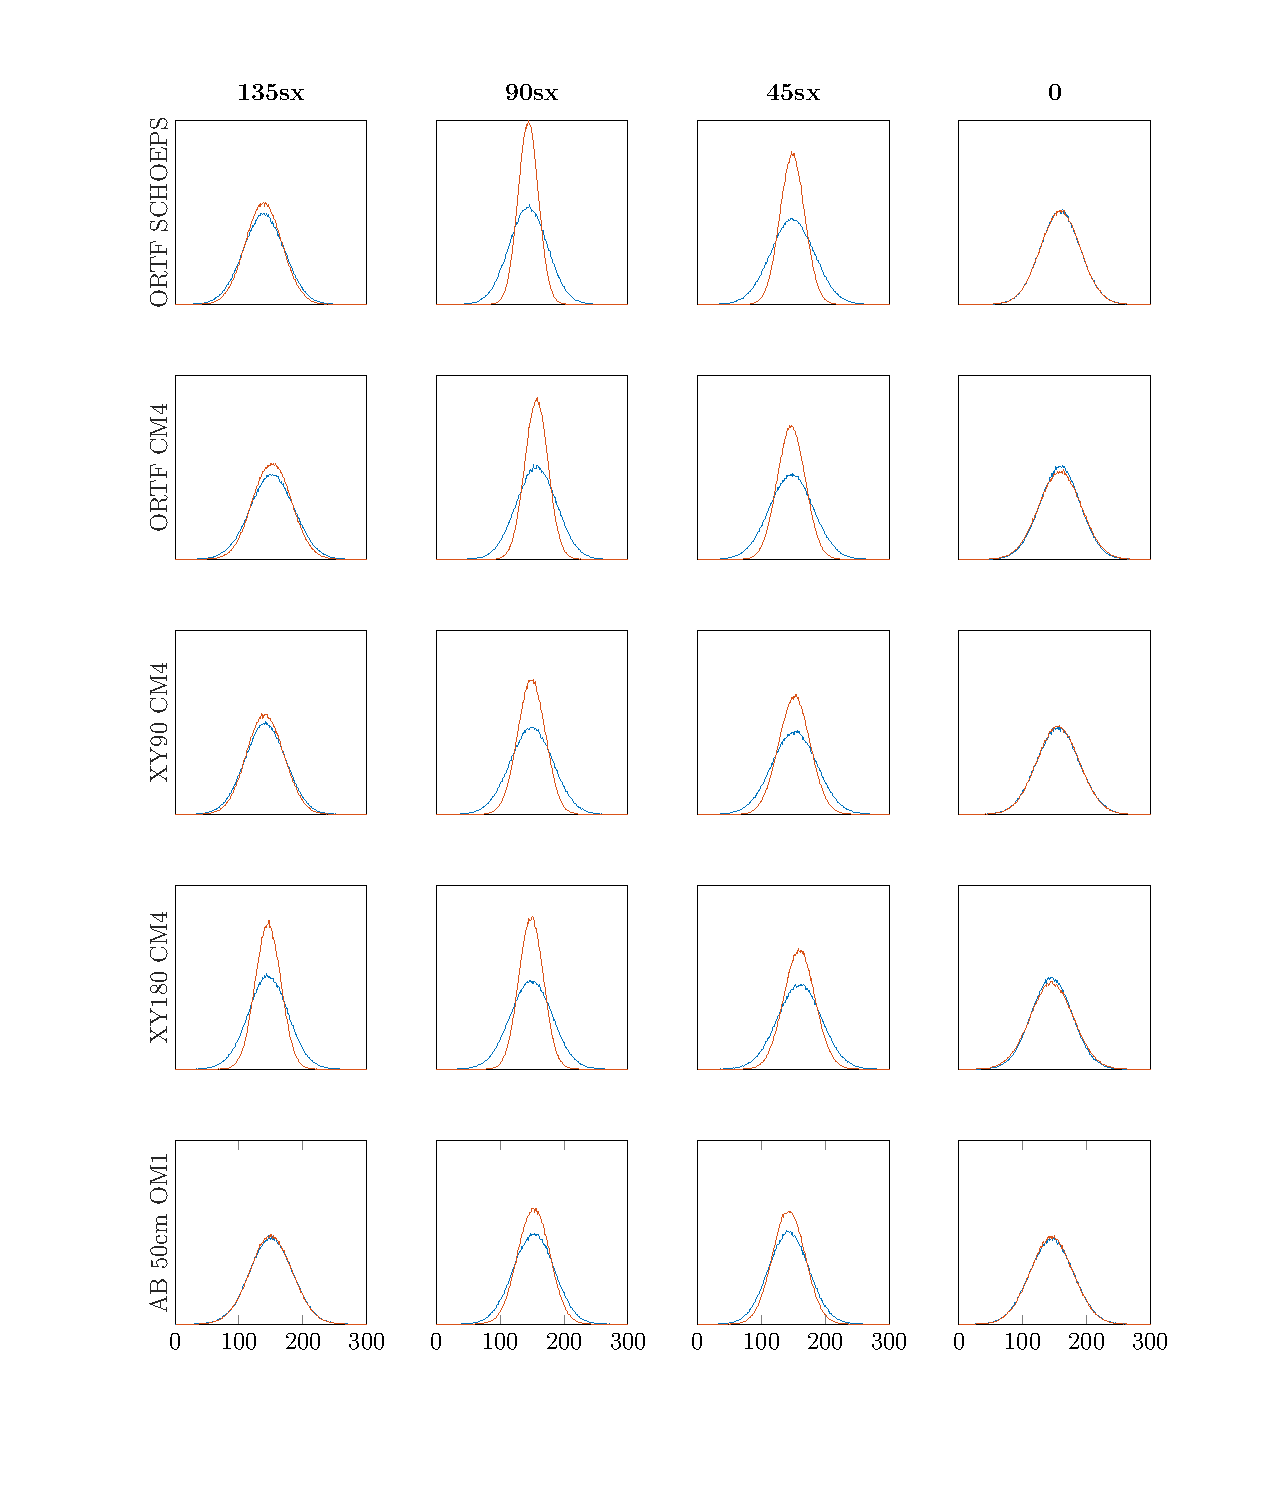
\includegraphics[width=.97\textwidth]{img/statistiche/pdf/amplitude_histograms_1}
  \caption{amplitude histograms.}
  \label{amphist1}
  \end{figure*}

\begin{figure*}[t]
  \centering
  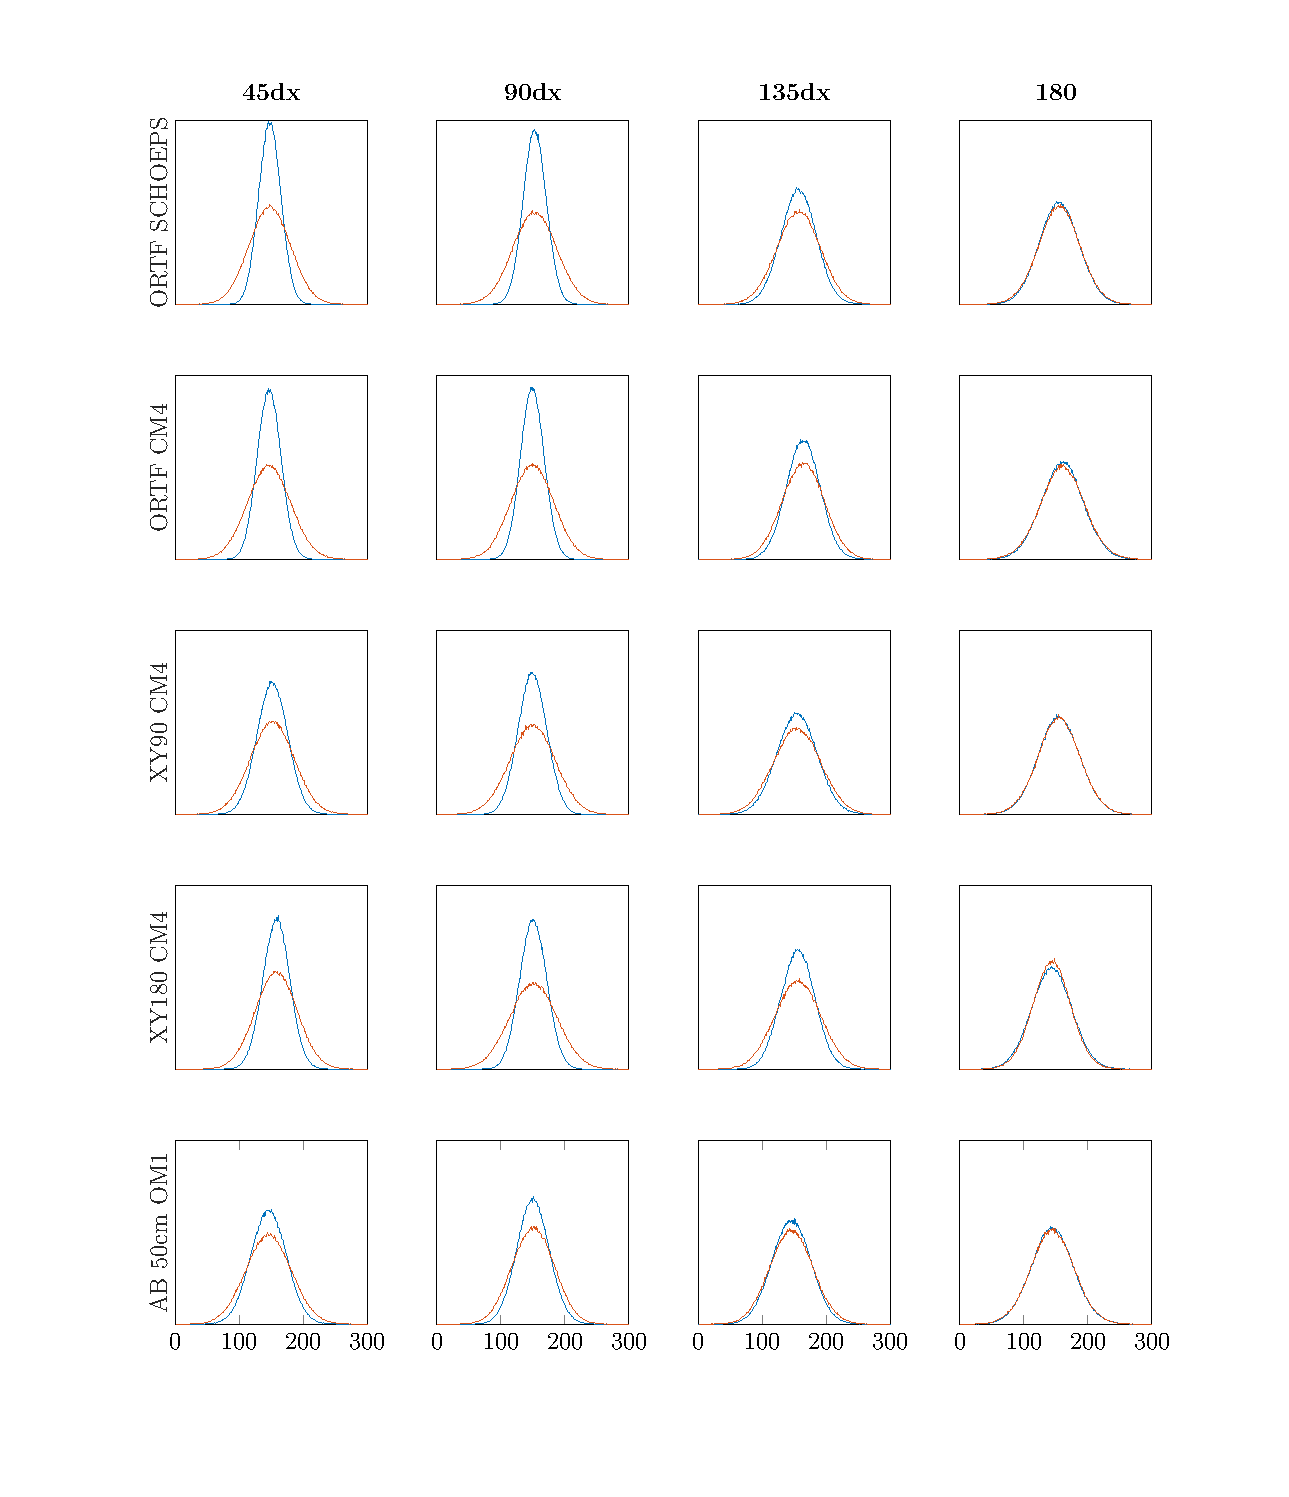
\includegraphics[width=.97\textwidth]{img/statistiche/pdf/amplitude_histograms_2}
  \caption{amplitude histograms.}
  \label{amphist2}
\end{figure*}

\begin{figure*}[t]
  \centering
  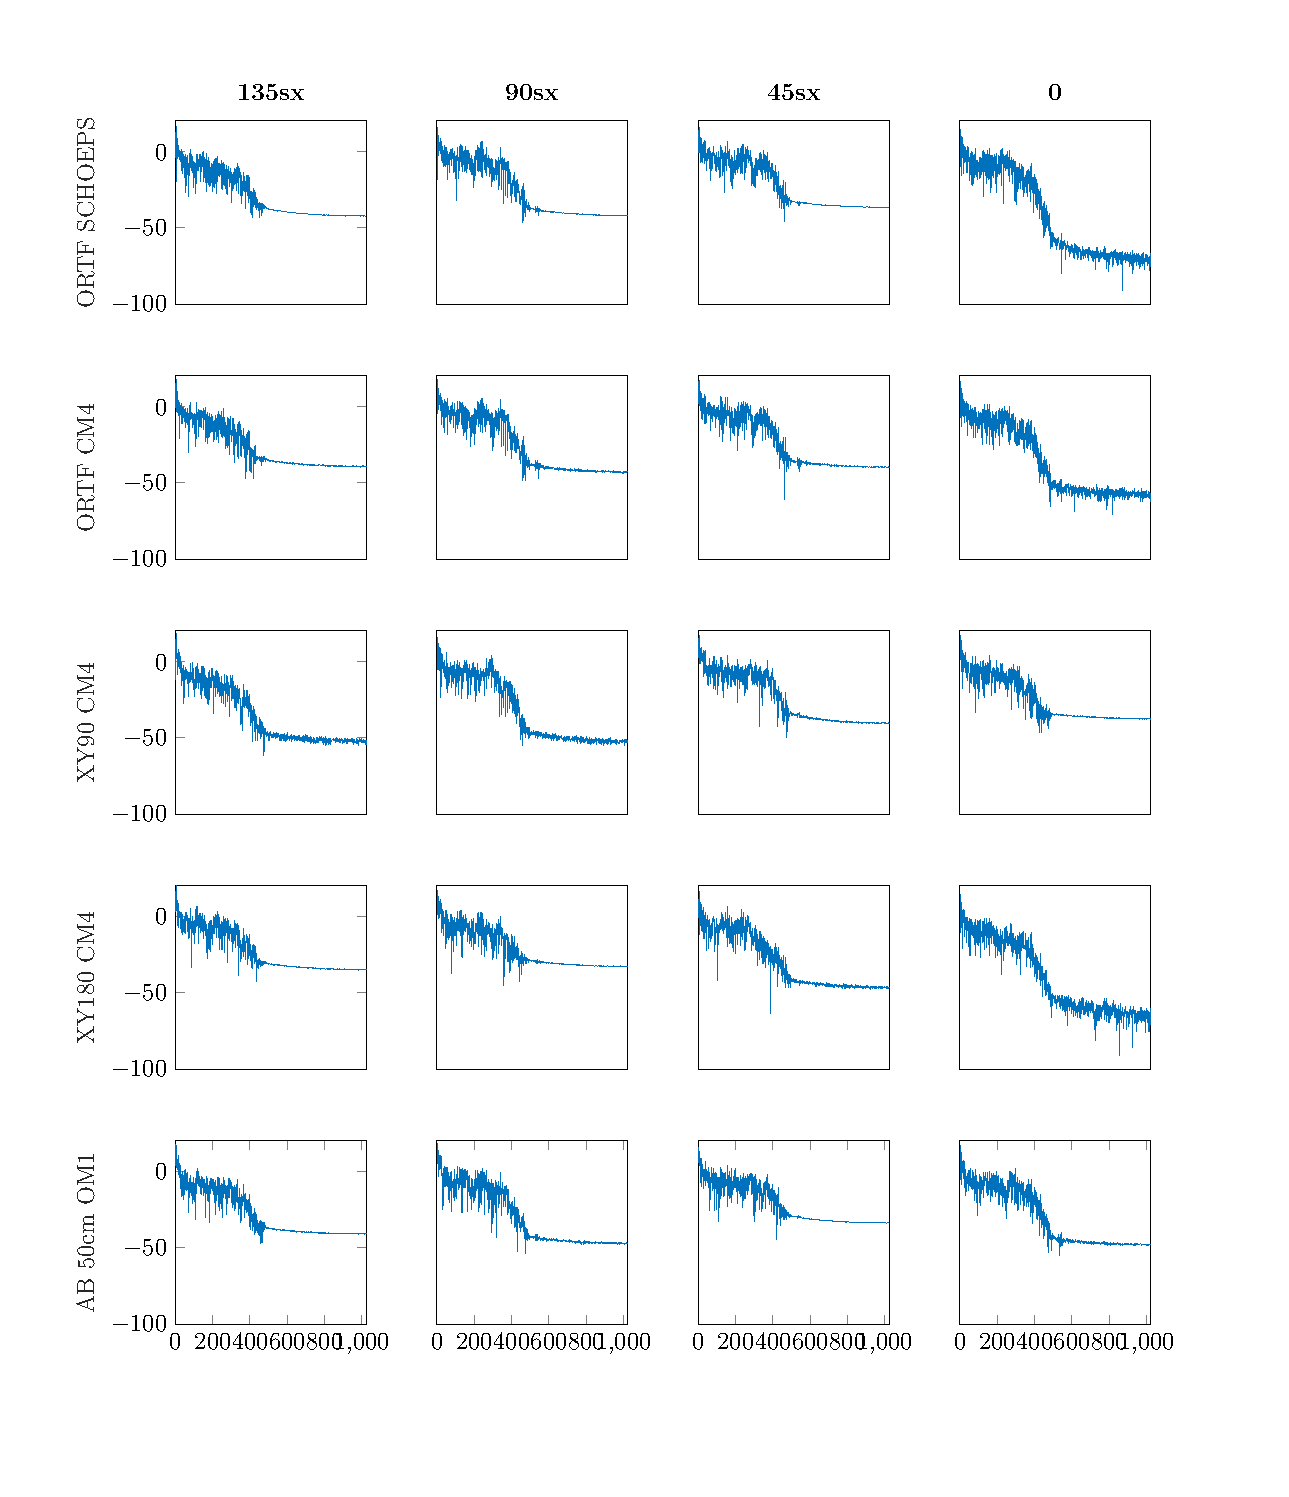
\includegraphics[width=.97\textwidth]{img/statistiche/pdf/spectra_1}
  \caption{spettri.}
  \label{spettri1}
\end{figure*}

\begin{figure*}[t]
  \centering
  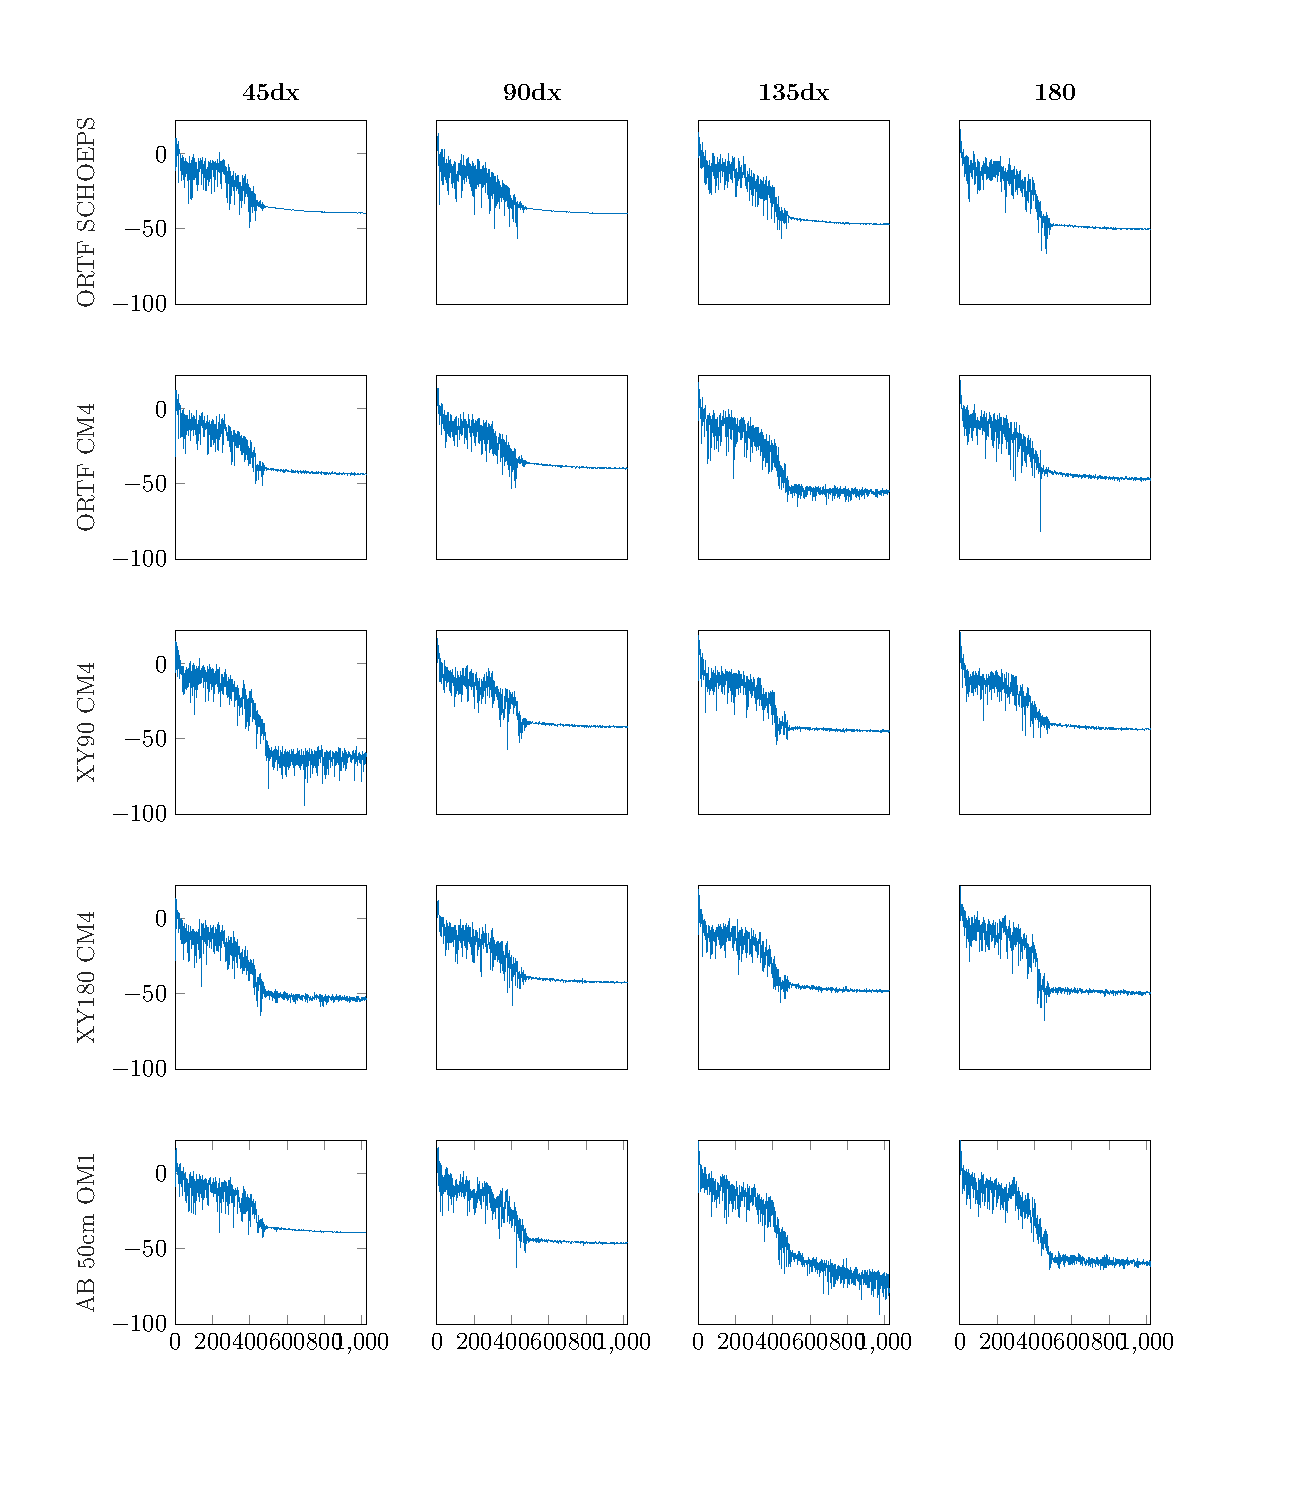
\includegraphics[width=.97\textwidth]{img/statistiche/pdf/spectra_2}
  \caption{spettri.}
  \label{spettri2}
\end{figure*}

Einstein's theory has important astrophysical implications. For example, it
implies the existence of black holes regions of space in which space and time
are distorted in such a way that nothing, not even light, can escape as an
end state for massive stars. There is ample evidence that the intense radiation
emitted by certain kinds of astronomical objects is due to black holes. For
example, microquasars and active galactic nuclei result from the presence of
stellar black holes and supermassive black holes, respectively. The bending of
light by gravity can lead to the phenomenon of gravitational lensing, in which
multiple images of the same distant astronomical object are visible in the sky.
General relativity also predicts the existence of gravitational waves, which
have since been observed directly by the physics collaboration LIGO. In addition,
general relativity is the basis of current cosmological models of a consistently
expanding universe.

\vfill\null

\raggedright
\bibliographystyle{unsrt}
\bibliography{includes/bibliography.bib}

\end{document}

%%%%%%%%%%%%%%%%%%%%%%%%%%%%%%%%%%%%%%%%%%%%%%%%%%%%%%%%%%%%%%%%%%%%%%%%%%%%%%%%
% 2020 GIUSEPPE SILVI ARTICLE TEMPLATE BASED ON
%%%%%%%%%%%%%%%%%%%%%%%%%%%%%%%%%%%%%%%%%%%%%%%%%%%%%%%%%%%%%%%%%%%%%%%%%%%%%%%%
% Journal Article
% LaTeX Template
% Version 1.4 (15/5/16)
% This template has been downloaded from:
% http://www.LaTeXTemplates.com
% Original author:
% Frits Wenneker (http://www.howtotex.com) with extensive modifications by
% Vel (vel@LaTeXTemplates.com)
% License:
% CC BY-NC-SA 3.0 (http://creativecommons.org/licenses/by-nc-sa/3.0/)
%%%%%%%%%%%%%%%%%%%%%%%%%%%%%%%%%%%%%%%%%%%%%%%%%%%%%%%%%%%%%%%%%%%%%%%%%%%%%%%%
